\documentclass[paper=letter,fontsize=11pt,titlepage,openany,twoside,
numbers=noenddot,index=totoc]{scrbook}
\usepackage[dvips]{graphicx}
\usepackage{float}
\usepackage[intoc]{nomencl}
\usepackage{xfrac}
\usepackage{fancybox}
\usepackage{pifont}
\usepackage{phaistos}
\usepackage{cancel}
\usepackage{amssymb}
\usepackage{amsmath}
\usepackage{amsthm}
\usepackage{empheq}
%\usepackage[dvips,gray]{xcolor}
\usepackage[dvips]{xcolor}
\usepackage[english]{babel}
\usepackage{fancyhdr}
\usepackage{fancyvrb}
\usepackage{shadethm}
\usepackage{makeidx}
\usepackage[T1]{fontenc}
\usepackage{fouriernc,bm}
\usepackage[scaled=0.80]{beramono}
\usepackage{ragged2e}
\usepackage{paralist}
\usepackage{mdwlist}
\usepackage{multicol}
\usepackage[labelsep=none]{caption}
\usepackage{subfig}
\usepackage{tikz}
\usetikzlibrary{arrows}
\usetikzlibrary{patterns}
\usetikzlibrary{decorations}
\usetikzlibrary{intersections}
\usetikzlibrary{matrix}
\usetikzlibrary{snakes}
\usetikzlibrary{calc}
\usetikzlibrary{backgrounds}
\usepackage{picins}
\usepackage{framed}
\usepackage{nextpage}
\usepackage{colortbl}
\usepackage{listings}
\lstloadlanguages{Gnuplot}
\usepackage[pdfproducer={GPL Ghostscript 9.06},pdfcreator={TeX Live 2012},
            pdfauthor={Michael Corral},pdftitle={Trigonometry},
            pdfsubject={Trigonometry},pdfkeywords={trigonometry},
            pdfdisplaydoctitle=true,dvips,bookmarks,pdfborder={0 0 0},
            bookmarksnumbered=true,colorlinks=false]{hyperref}
\usepackage{breakurl}

% Set the sans serif font to Helvetica (for chapter and section headings)
\renewcommand\sfdefault{phv}

\definecolor{captioncolor}{HTML}{005587}
\definecolor{linecolor}{HTML}{0074C8}
\definecolor{fillcolor}{cmyk}{0.1,0.05,0,0}
\definecolor{brickcolor}{HTML}{F0D8B2}
\definecolor{blockcolor}{HTML}{B6B6B6}
\definecolor{groundcolor}{HTML}{E4D8C5}
\definecolor{earthcolor}{HTML}{C5FFFF}
\definecolor{watercolor}{cmyk}{0.1,0.05,0,0}
\definecolor{codecolor}{HTML}{FFF7E0}
\definecolor{linenumcolor}{HTML}{8C8C8C}
%\definecolor{headercolor}{HTML}{F5F5F5}
\definecolor{headercolor}{HTML}{E9EFEF}
\DeclareCaptionFont{blue}{\color{captioncolor}}
\captionsetup{labelfont={bf,blue},font={small,blue},textfont={small,blue}}
\providecommand{\lineacross}{\hrule width \textwidth height 0.5pt}
\newcommand{\startexercises}{
 \centerline{\fbox{\textsf{\textbf{\large Exercises}}}}
}
\newcommand{\probs}[1]{\par\noindent\textsf{\textbf{\large #1}}}
\newcommand{\hrulethick}{\leaders\hrule height 5pt depth -2pt\hfill}
\newcommand{\divider}{\noindent{\color{linecolor}\rule{\linewidth}{3pt}}}
\setlength{\multicolsep}{2.5mm}
\setlength{\leftmargini}{1.4em}
\setlength{\shadeboxrule}{.4pt}
\theoremstyle{definition}
\newshadetheorem{defn}{Definition}[chapter]
\newshadetheorem{thm}{Theorem}[chapter]
\newshadetheorem{lem}[thm]{Lemma}
\newshadetheorem{cor}[thm]{Corollary}
\newtheoremstyle{itexmp}%
 {\topsep}
 {\topsep}
 {\normalfont\small}
 {0pt}
 {\itshape\bfseries}{}
 { }
 {#1 \textbf{#2} \enskip {\color{linecolor}\hrulethick}\\[6pt]}
\theoremstyle{itexmp}
\newtheorem{exmp}{Example}[chapter]
\newcommand{\statedefn}[2]{
 \definecolor{shadethmcolor}{HTML}{EDF8FF}
 \definecolor{shaderulecolor}{cmyk}{0.73,0.19,0,0}
 \begin{defn}\label{#1}{#2}\end{defn}
}
\newcommand{\statethm}[2]{
 \definecolor{shadethmcolor}{HTML}{FFFFD8}
 \definecolor{shaderulecolor}{HTML}{9B5900}
 \begin{thm}\label{#1}{#2}\end{thm}
}
\newcommand{\statecor}[2]{
 \definecolor{shadethmcolor}{HTML}{FAF2FF}
 \definecolor{shaderulecolor}{HTML}{9B5900}
 \begin{cor}\label{#1}{#2}\end{cor}
}
\newcommand{\statecomment}[2][0.96\textwidth]{
 \par\noindent\tikzstyle{mybox} = [draw=green!70!black,fill=green!5,thick,rectangle,rounded corners,inner ysep=4pt]
 \begin{tikzpicture}
  \node [mybox] (box){%
   \begin{minipage}{#1}{#2}\end{minipage}
  };
 \end{tikzpicture}
}
\newcommand*\widefbox[1]{\fbox{\hspace{1em}#1\hspace{1em}}}
\renewcommand{\CancelColor}{\color{red}}
\newcommand\myclearpage{\cleartooddpage
 [\thispagestyle{empty}]}
\providecommand{\abs}[1]{\lvert\mspace{1mu}#1\mspace{1mu}\rvert}
\providecommand{\Abs}[1]{\bigl\lvert\mspace{1mu}#1\mspace{1mu}\bigr\rvert}
\providecommand{\norm}[1]{\lVert\mspace{1mu}#1\mspace{1mu}\rVert}
\providecommand{\Norm}[1]{\bigl\lVert\mspace{1mu}#1\mspace{1mu}\bigr\rVert}
\providecommand{\NORM}[1]{\Biggl\lVert\mspace{1mu}#1\mspace{1mu}\Biggr\rVert}
\providecommand{\ssub}[2]{#1_{\scriptscriptstyle #2}}
\providecommand{\ssubsum}[3]{#1_{\scriptscriptstyle #3} + #2_{\scriptscriptstyle #3}}
\providecommand{\Reals}{\mathbb{R}}
\providecommand{\Complex}{\mathbb{C}}
\providecommand{\Rationals}{\mathbb{Q}}
\providecommand{\Naturals}{\mathbb{N}}
\providecommand{\Integers}{\mathbb{Z}}
\providecommand{\Degrees}[0]{\ensuremath{^\circ}}
\providecommand{\ival}[2]{\lbrack #1,#2 \rbrack}
%\newcommand{\calcbutton}[1]{\setlength\fboxsep{1pt}\cornersize{1}\ovalbox{\small #1}}
%\newcommand{\calcbutton}[1]{\ovalbox{\small #1}}
\newenvironment{proofbar}{%
  \def\FrameCommand{\vrule width 1pt \hspace{5pt}}%
  \MakeFramed {\advance\hsize-\width \FrameRestore}}%
 {\endMakeFramed}
\allowdisplaybreaks[1]
\numberwithin{figure}{section}
\setlength\oddsidemargin{20pt}
\setlength\evensidemargin{20pt}
\setlength\topmargin{0pt}
\setlength\headsep{10pt}
\setlength\textheight{202mm}
%Change indent after chapter number in TOC from 1.5em to 2.2em, and from 2.3 to 3.0 for sections
\makeatletter
\renewcommand*\l@chapter[2]{%
  \ifnum \c@tocdepth >\m@ne
    \addpenalty{-\@highpenalty}%
    \vskip 1.0em \@plus\p@
    \setlength\@tempdima{2.2em}%
    \if@tocleft
      \ifx\toc@l@number\@empty\else
        \setlength\@tempdima{0\toc@l@number}%
      \fi
    \fi
    \begingroup
      \parindent \z@ \rightskip \@pnumwidth
      \parfillskip -\@pnumwidth
      \leavevmode \sectfont
      \advance\leftskip\@tempdima
      \hskip -\leftskip
      #1\nobreak\hfil \nobreak\hb@xt@\@pnumwidth{\hss #2}\par
      \penalty\@highpenalty
    \endgroup
  \fi}
\renewcommand*\l@section{\@dottedtocline{1}{2.2em}{3.0em}}
\makeatother
\makeindex
\makenomenclature
\begin{document}
\deffootnote[1em]{0em}{1em}{\textsuperscript{\thefootnotemark}}
\frontmatter
\pagestyle{empty}
%Put the front cover here
\thisfancypage{\setlength{\fboxsep}{1pt}\setlength\fboxrule{1.5pt}\fbox}{}


\includegraphics{cover-top}\vspace{14mm}

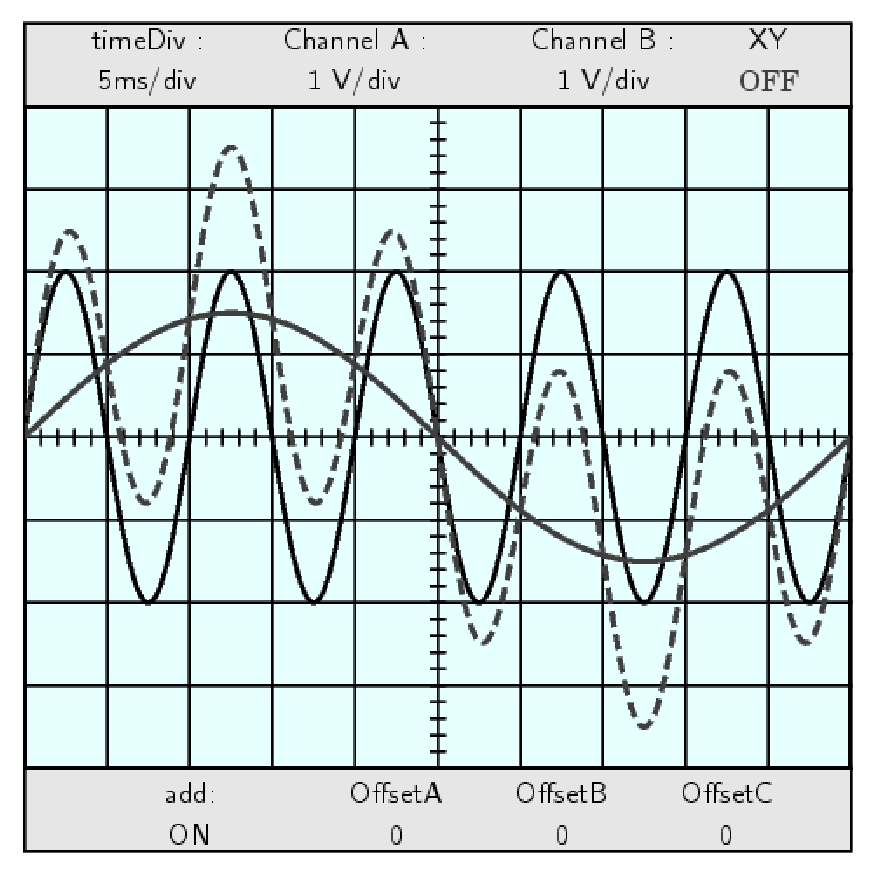
\includegraphics{osci-large-color}

%Put the title page here
\title{Trigonometry}
\author{\textsf{\textbf{Michael Corral}}}
\date{\large \textsf{\textsl{Schoolcraft College}}}
%Put the author/copyright info here
\uppertitleback{\emph{About the author}:\\
Michael Corral is an Adjunct Faculty member of the Department of Mathematics at Schoolcraft College. 
He received a B.A. in Mathematics from the University of California at Berkeley, and received an M.A. in Mathematics and
an M.S. in Industrial \& Operations Engineering from the University of Michigan.\\\\
This text was typeset in \LaTeX\medspace with the \textsf{KOMA-Script} bundle, using the GNU Emacs text editor on a
Fedora Linux system. The graphics were created using TikZ and Gnuplot.}
\lowertitleback{Copyright \copyright ~2009 ~Michael Corral.\\
Permission is granted to copy, distribute and/or modify this document
under the terms of the GNU Free Documentation License, Version 1.3
or any later version published by the Free Software Foundation;
with no Invariant Sections, no Front-Cover Texts, and no Back-Cover
Texts. A copy of the license is included in the section entitled ``GNU
Free Documentation License.''}
\maketitle
\pagestyle{fancy}
\addtokomafont{footnotelabel}{\color{linecolor}}
\addtokomafont{footnotereference}{\color{linecolor}}
\renewcommand{\chaptermark}[1]{\markboth{#1}{}}
\renewcommand{\sectionmark}[1]{\markright{#1}}
\renewcommand{\qedsymbol}{\textsf{\textbf{\textsc{\small{qed}}}}}
\fancyhf{}
\setlength{\headheight}{22.26332pt}
\renewcommand{\headrulewidth}{0pt}
\newlength{\fminilength}%
\setlength{\fminilength}{\textwidth-2\fboxsep-2\fboxrule}%
\fancyhf{}
\fancyhead[LE]{\small\thepage}
\fancyhead[CE]{\small\scshape\leftmark}
\fancyhead[RO]{\small\thepage}
\fancyhead[CO]{\small\scshape\leftmark}
%Put the preface here
\addchap{Preface}
This book covers elementary trigonometry. It is suitable for a one-semester course at the college
level, though it could also be used in high schools. The prerequisites are high school algebra and
geometry.

This book basically consists of my lecture notes from teaching trigonometry at Schoolcraft College
over several years, expanded with some exercises. There are exercises at the end of each section.
I have tried to include some
more challenging problems, with hints when I felt those were needed. An average student should be
able to do most of the exercises. Answers and hints to many of the odd-numbered and some of the
even-numbered exercises are provided in Appendix A.

This text probably has a more geometric feel to it than most current trigonometry texts.
That was, in fact, one of the reasons I wanted to write this book. I think that approaching the
subject with too much of an analytic emphasis is a bit confusing to students. It makes much of the
material appear unmotivated. This book starts with the ``old-fashioned'' right triangle approach to
the trigonometric functions, which is more intuitive for students to grasp.

In my experience, presenting the definitions of the trigonometric
functions and then immediately jumping into proving identities is too much of a detour from
geometry to analysis for most students.
So this book presents material in a very different order than most books today. For
example, after starting with the right triangle definitions and some applications, general (oblique)
triangles are presented. That seems like a more natural progression of topics, instead of leaving
general triangles until the end as is usually the case.

The goal of this book is a bit different, too. Instead of taking the (doomed) approach that students
have to be shown that trigonometry is ``relevant to their everyday lives'' (which inevitably comes
off as artificial), this book has a different mindset:
\emph{preparing students to use trigonometry as it is used in other courses}.
Virtually no students will ever in their ``everyday life'' figure out the height of a tree
with a protractor or determine the angular speed of a Ferris wheel.
Students are far more likely to need trigonometry in other courses (e.g. engineering, physics).
I think that math instructors have a duty to prepare students for that.

In Chapter 5 students are asked to use the free open-source software Gnuplot to graph
some functions. However, any program can be used for those exercises, as long as it produces
accurate graphs. Appendix B contains a brief tutorial on Gnuplot.

There are a few exercises that require the student to write his or her own computer program
to solve some numerical computation problems. There
are a few code samples in Chapter 6, written in the Java and Python programming languages, hopefully
sufficiently clear so that the reader can figure out what is being done even without knowing those
languages. Octave and Sage are also mentioned. This book probably discusses numerical issues more
than most texts at this level (e.g. the numerical instability of Heron's formula for the area of a
triangle, the secant method for solving trigonometric equations). Numerical methods probably should
have been emphasized even more in the text, since it is rare when even a moderately complicated
trigonometric equation can be solved with elementary methods, and since mathematical software is
so readily available.

I wanted to keep this book as brief as possible. Someone once joked that trigonometry is two weeks
of material spread out over a full semester, and I think that there is some truth to that.
However, some decisions had to be made on what material to leave out. I had planned to include
sections on vectors, spherical trigonometry - a subject which has basically vanished from
trigonometry texts in the last few decades (why?) - and a few other topics, but decided against it.
The hardest decision was to exclude Paul Rider's clever geometric proof of the Law of Tangents
without using any sum-to-product identities, though I do give a reference to it.

This book is released under the GNU Free Documentation License (GFDL), which allows others to not
only copy and distribute the book but also to modify it. For more details, see the included copy of
the GFDL. So that there is no ambiguity on this matter, anyone can make as many copies of this book
as desired and distribute it as desired, without needing my permission. The PDF version will always
be freely available to the public at no cost (go to \url{http://www.mecmath.net/trig}). Feel free to
contact me at \texttt{\href{mailto:mcorral@schoolcraft.edu}{mcorral@schoolcraft.edu}} for any
questions on this or any other matter involving the book (e.g. comments, suggestions, corrections,
etc). I welcome your input.

\begin{flushleft}
\emph{July 2009}\hspace{\stretch{1}}\textsc{Michael Corral}\\
\emph{Livonia, Michigan}
\end{flushleft}

%\thispagestyle{empty}
\pdfbookmark[0]{\contentsname}{toc}
%Put the table of contents here
\tableofcontents
%Put a completely blank page here if the TOC has an odd number of pages
\clearpage{\pagestyle{empty}\cleardoublepage}
\mainmatter
\fancyhf{}
\fancyhead[LE]{\tikzstyle{headbox} = [fill=headercolor,line width=0pt,rectangle,rounded corners]
 \begin{tikzpicture}
  \node [headbox] (box){%
   \begin{minipage}{\fminilength}%
     \sffamily{\bfseries\thepage\qquad Chapter \thechapter}\enskip $\bullet$ \enskip\leftmark\hfill{\bfseries\S\thesection}
    \end{minipage}%
  };
 \end{tikzpicture}}
\fancyhead[LO]{\tikzstyle{headbox} = [fill=headercolor,line width=0pt,rectangle,rounded corners]
 \begin{tikzpicture}
  \node [headbox] (box){%
   \begin{minipage}{\fminilength}%
     \sffamily {}\hfill\rightmark\enskip $\bullet$ \enskip{\bfseries{Section \thesection\qquad\thepage}}
    \end{minipage}%
  };
 \end{tikzpicture}}
%Put the main chapters here
\chapter{Right Triangle Trigonometry}
Trigonometry is the study of the relations between the sides and angles of triangles. The word
``trigonometry'' is derived from the Greek words \emph{trigono}
($\othertau\otherrho\acute{\otheriota}\othergamma\otheromega\othernu$o), meaning ``triangle'', and \emph{metro}
($\othermu\otherepsilon\othertau\otherrho\acute{\otheromega}$), meaning ``measure''. Though the ancient Greeks,
such as Hipparchus\index{Hipparchus} and Ptolemy\index{Ptolemy}, used trigonometry in their study of
astronomy between roughly 150 \textsc{b.c.} - \textsc{a.d.} 200, its history is much older.
For example, the Egyptian scribe Ahmes\index{Ahmes} recorded some rudimentary
trigonometric calculations (concerning ratios of sides of pyramids) in the famous Rhind
Papyrus\index{Rhind Papyrus} sometime around 1650 \textsc{b.c.}\footnote{Ahmes claimed that he
copied the papyrus from a work that may date as far back as 3000 \textsc{b.c.}}

Trigonometry is distinguished from elementary geometry in part by its extensive use of certain
functions of angles, known as the \emph{trigonometric functions}. Before discussing those functions,
we will review some basic terminology about angles.

%Begin Section 1.1
\section{Angles}
Recall the following definitions from elementary geometry:\index{angle}
\begin{enumerate}[\bfseries (a)]
 \item An angle is \textbf{acute}\index{acute angle}\index{angle!acute} if it is between $0\Degrees$
  and $90\Degrees$.
 \item An angle is a \textbf{right angle}\index{right angle}\index{angle!right} if it equals
  $90\Degrees$.
 \item An angle is \textbf{obtuse}\index{obtuse angle}\index{angle!obtuse} if it is between
  $90\Degrees$ and $180\Degrees$.
 \item An angle is a \textbf{straight angle}\index{straight angle}\index{angle!straight} if it
  equals $180\Degrees$.
\end{enumerate}

\begin{figure}[h]
 \centering
 \subfloat[][ acute angle]{
 \begin{tikzpicture}
  \draw [line width=0.5pt,-latex] (0.7,0) arc (0:45:0.7);
  \draw [linecolor,line width=1.5pt,latex-latex] (1.5,0) -- (0,0) -- (1.3,1.3);
  \draw [white] (1.6,0) -- (2.1,0);
  \draw [white] (-0.1,0) -- (-0.5,0);
 \end{tikzpicture}}
 \qquad
 \subfloat[][ right angle]{
 \begin{tikzpicture}
  \draw [line width=0.5pt,-latex] (0.7,0) arc (0:90:0.7);
  \draw [line width=0.5pt] (0.2,0) -- (0.2,0.2) -- (0,0.2);
  \draw [linecolor,line width=1.5pt,latex-latex] (1.5,0) -- (0,0) -- (0,1.3);
  \draw [white] (1.6,0) -- (2.1,0);
  \draw [white] (-0.1,0) -- (-0.5,0);
 \end{tikzpicture}}
 \qquad
 \subfloat[][ obtuse angle]{
 \begin{tikzpicture}
  \draw [line width=0.5pt,-latex] (0.7,0) arc (0:135:0.7);
  \draw [linecolor,line width=1.5pt,latex-latex] (1.5,0) -- (0,0) -- (-1.3,1.3);
 \end{tikzpicture}}
 \qquad
 \subfloat[][ straight angle]{
 \begin{tikzpicture}
  \draw [line width=0.5pt,-latex] (0.7,0) arc (0:180:0.7);
  \draw [linecolor,line width=1.5pt,latex-latex] (-1.5,0) -- (0,0) -- (1.5,0);
 \end{tikzpicture}}
 \caption[]{\quad Types of angles}
 \label{fig:angles}
\end{figure}

In elementary geometry, angles are always considered to be positive and not larger than
$360\Degrees$. For now we will only consider such angles.\footnote{Later in the text we will
discuss negative angles and angles larger than $360\Degrees$.} The following definitions will be
used throughout the text:
\newpage
\begin{enumerate}[\bfseries (a)]
 \item Two acute angles are \textbf{complementary}\index{complementary angles} if their sum equals
  $90\Degrees$. In other words, if $0\Degrees \le \angle\,A \,,\, \angle\,B \le 90\Degrees$ then
  $\angle\,A$ and $\angle\,B$ are complementary if $\angle\,A + \angle\,B = 90\Degrees$.
 \item Two angles between $0\Degrees$ and $180\Degrees$ are
  \textbf{supplementary}\index{supplementary angles} if their sum equals $180\Degrees$. In other
  words, if $0\Degrees \le \angle\,A \,,\, \angle\,B \le 180\Degrees$ then $\angle\,A$ and
  $\angle\,B$ are supplementary if $\angle\,A + \angle\,B = 180\Degrees$.
 \item Two angles between $0\Degrees$ and $360\Degrees$ are \textbf{conjugate}\index{conjugate
  angles} (or \textbf{explementary}\index{explementary angles}) if their sum equals $360\Degrees$.
  In other words, if $0\Degrees \le \angle\,A \,,\, \angle\,B
  \le 360\Degrees$ then $\angle\,A$ and $\angle\,B$ are conjugate if $\angle\,A + \angle\,B =
  360\Degrees$.
\end{enumerate}

\begin{figure}[h]
 \centering
 \subfloat[][ complementary]{
 \begin{tikzpicture}
  \draw [line width=0.5pt,latex-] (0,1) arc (90:56.3:1);
  \draw [line width=0.5pt,-latex] (1,0) arc (0:56.3:1);
  \draw [line width=0.5pt] (0.2,0) -- (0.2,0.2) -- (0,0.2);
  \draw [linecolor,line width=1.5pt,latex-latex] (1.5,0) -- (0,0) -- (0,1.8);
  \draw [linecolor,line width=1.5pt,-latex] (0,0) -- (1,1.5);
  \draw [white] (1.6,0) -- (2.3,0);
  \draw [white] (-0.1,0) -- (-0.7,0);
  \node [right] at (0.85,0.6) {\small $\angle\,A$};
  \node [above] at (0.35,1) {\small $\angle\,B$};
 \end{tikzpicture}}
 \qquad\qquad
 \subfloat[][ supplementary]{
 \begin{tikzpicture}
  \draw [line width=0.5pt,-latex] (0.7,0) arc (0:135:0.7);
  \draw [line width=0.5pt,latex-] (-0.7,0) arc (180:135:0.7);
  \draw [linecolor,line width=1.5pt,latex-latex] (-1.8,0) -- (1.8,0);
  \draw [linecolor,line width=1.5pt,-latex] (0,0) -- (-1.3,1.3);
  \node [above right] at (0.1,0.8) {\small $\angle\,A$};
  \node [above left] at (-0.65,0.25) {\small $\angle\,B$};
 \end{tikzpicture}}
 \qquad\qquad
 \subfloat[][ conjugate]{
 \begin{tikzpicture}
  \draw [line width=0.5pt,latex-] (0.7,0) arc (360:56.3:0.7);
  \draw [line width=0.5pt,-latex] (0.7,0) arc (0:56.3:0.7);
  \draw [linecolor,line width=1.5pt,latex-latex] (1.5,0) -- (0,0) -- (1,1.5);
  \node [right] at (0.8,0.5) {\small $\angle\,A$};
  \node [above] at (-0.7,0.5) {\small $\angle\,B$};
 \end{tikzpicture}}
 \caption[]{\quad Types of pairs of angles}
 \label{fig:angles2}
\end{figure}\vspace{-2mm}

Instead of using the angle notation $\angle\,A$ to denote an angle, we will sometimes use just a
capital letter by itself (e.g. $A$, $B$, $C$) or a lowercase variable name (e.g. $x$, $y$, $t$).
It is also common to use letters (either uppercase or lowercase) from the Greek alphabet, shown
in the table below, to represent angles:\index{Greek alphabet}\vspace{-3mm}

\begin{table}[h]\centering
\caption{\quad \textbf{The Greek alphabet}}\vspace{3mm}
\begin{tabular}{lll!{\qquad\qquad}lll!{\qquad\qquad}lll}
\hline\\[0.5pt]
\multicolumn{2}{l}{\textbf{Letters}} & \textbf{Name} & \multicolumn{2}{l}{\textbf{Letters}} &
 \textbf{Name} & \multicolumn{2}{l}{\textbf{Letters}} & \textbf{Name}\\[4pt]
A & $\alpha$ & alpha & I & $\iota$ & iota & P & $\rho$ & rho\\
B & $\beta$ & beta & K & $\kappa$ & kappa & $\Sigma$ & $\sigma$ & sigma\\
$\Gamma$ & $\gamma$ & gamma & $\Lambda$ & $\lambda$ & lambda & T & $\tau$ & tau\\
$\Delta$ & $\delta$ & delta & M & $\mu$ & mu & $\Upsilon$ & $\upsilon$ & upsilon\\
E & $\epsilon$ & epsilon & N & $\nu$ & nu & $\Phi$ & $\phi$ & phi\\
Z & $\zeta$ & zeta & $\Xi$ & $\xi$ & xi & X & $\chi$ & chi\\
H & $\eta$ & eta & O & $o$ & omicron & $\Psi$ & $\psi$ & psi\\
$\Theta$ & $\theta$ & theta & $\Pi$ & $\pi$ & pi & $\Omega$ & $\omega$ & omega\\[1pt]\\
\hline
\end{tabular}
\end{table}

In elementary geometry you learned that the sum of the angles in a triangle equals $180\Degrees$,
and that an \textbf{isosceles triangle}\index{isosceles triangle}\index{triangle!isosceles} is a
triangle with two sides of equal length.
Recall that in a \textbf{right triangle}\index{right triangle}\index{triangle!right} one of the
angles is a right angle. Thus, in a right triangle\index{triangle} one of the angles is
$90\Degrees$ and the other two angles are acute angles whose sum is $90\Degrees$ (i.e. the other two
angles are complementary angles).
\newpage
\begin{exmp}
 For each triangle below, determine the unknown angle(s):
  \begin{center}
  \begin{tikzpicture}
   \filldraw [linecolor,line width=1.5pt,fill=fillcolor] (0,0) -- (4,0) -- (35:1.7) -- cycle;
   \node [below left] at (0,0) {\small $A$};
   \node [above] at (35:1.7) {\small $B$};
   \node [below right] at (4,0) {\small $C$};
   \node at (15:0.75) {\small $35\Degrees$};
   \node at (2.8,0.2) {\small $20\Degrees$};

   \filldraw [linecolor,line width=1.5pt,fill=fillcolor] (6,0) -- (8,0) -- (8,1.5) -- cycle;
   \draw (7.8,0.025) -- (7.8,0.23) -- (7.975,0.23);
   \node [below left] at (6,0) {\small $D$};
   \node [above right] at (8,1.5) {\small $E$};
   \node [below right] at (8,0) {\small $F$};
   \node at (7.7,0.9) {\small $53\Degrees$};

   \filldraw [linecolor,line width=1.5pt,fill=fillcolor] (10,0) -- (13,0) -- (11.5,1.3) -- cycle;
   \node [below left] at (10,0) {\small $X$};
   \node [above] at (11.5,1.3) {\small $Y$};
   \node [below right] at (13,0) {\small $Z$};
   \node at (10.5,0.2) {\small $\alpha$};
   \node at (12.5,0.2) {\small $\alpha$};
   \node at (11.5,1) {\small $3\alpha$};
  \end{tikzpicture}
 \end{center}
\par\noindent Note: We will sometimes refer to the angles of a triangle by their vertex
points. For example, in the first triangle above we will simply refer to the angle $\angle\,BAC$
as angle $A$.\vspace{1mm}
\par\noindent\textbf{Solution:} For triangle $\triangle\,ABC$, $A = 35\Degrees$ and $C = 20\Degrees$,
and we know that $A + B + C = 180\Degrees$, so
 \begin{displaymath}
  35\Degrees ~+~ B ~+~ 20\Degrees ~=~ 180\Degrees \quad\Rightarrow\quad B ~=~ 180\Degrees ~-~
   35\Degrees ~-~ 20\Degrees \quad\Rightarrow\quad \fbox{$B ~=~ 125\Degrees$} ~.
 \end{displaymath}
 For the right triangle $\triangle\,DEF$, $E = 53\Degrees$ and $F = 90\Degrees$, and we know that
 the two acute angles $D$ and $E$ are complementary, so
 \begin{displaymath}
  D ~+~ E ~=~ 90\Degrees \quad\Rightarrow\quad D ~=~ 90\Degrees ~-~
   53\Degrees \quad\Rightarrow\quad \fbox{$D ~=~ 37\Degrees$} ~.
 \end{displaymath}
 For triangle $\triangle\,XYZ$, the angles are in terms of an unknown number $\alpha$, but we do
 know that $X + Y + Z = 180\Degrees$, which we can use to solve for $\alpha$ and then use that to
 solve for $X$, $Y$, and $Z$:
 \begin{displaymath}
  \alpha ~+~ 3\alpha ~+~ \alpha ~=~ 180\Degrees \quad\Rightarrow\quad 5\alpha ~=~ 180\Degrees
  \quad\Rightarrow\quad \alpha ~=~ 36\Degrees \quad\Rightarrow\quad \fbox{$X = 36\Degrees ~,~
  Y = 3 \times 36\Degrees = 108\Degrees ~,~ Z = 36\Degrees$}
 \end{displaymath}
\end{exmp}
\begin{exmp}
 \emph{Thales' Theorem} states that if $A$, $B$, and $C$ are (distinct) points on a circle such that
 the line segment $\overline{AB}$ is a diameter of the circle, then the angle $\angle\,ACB$ is a
 right angle (see Figure \ref{fig:thales}(a)). In other words, the triangle $\triangle\,ABC$ is a
 right triangle.\index{Thales' Theorem}\vspace{-2mm}

\begin{figure}[h]
 \centering
 \subfloat[][]{
  \begin{tikzpicture}[scale=0.8]
   \filldraw [linecolor,fill=fillcolor,line width=1.5pt] (-2,0) -- (2,0) -- (70:2) -- (-2,0);
   \draw [line width=0.5pt] (0,0) circle (2);
   \node [left] at (-2,0) {\small $A$};
   \node [right] at (2,0) {\small $B$};
   \node [above] at (70:2) {\small $C$};
   \node [below] at (0,0) {\small $O$};
   \fill (-2,0) circle (2pt);
   \fill (2,0) circle (2pt);
   \fill (70:2) circle (2pt);
   \fill (0,0) circle (2pt);
  \end{tikzpicture}}
 \qquad\qquad
 \subfloat[][]{
  \begin{tikzpicture}[scale=0.8]
   \filldraw [linecolor,fill=fillcolor,line width=1.5pt] (-2,0) -- (2,0) -- (70:2) -- (-2,0);
   \draw [line width=0.5pt] (0,0) circle (2);
   \draw [line width=0.5pt] (0,0) -- (70:2);
   \node [left] at (-2,0) {\small $A$};
   \node [right] at (2,0) {\small $B$};
   \node [above] at (70:2) {\small $C$};
   \node [below] at (0,0) {\small $O$};
   \node at (-1.3,0.2) {\small $\alpha$};
   \node at (77:1.4) {\small $\alpha$};
   \node at (62:1.52) {\small $\beta$};
   \node at (1.5,0.2) {\small $\beta$};
   \fill (-2,0) circle (2pt);
   \fill (2,0) circle (2pt);
   \fill (70:2) circle (2pt);
   \fill (0,0) circle (2pt);
  \end{tikzpicture}}
 \caption[]{\quad Thales' Theorem: $\angle\,ACB = 90\Degrees$}
 \label{fig:thales}
\end{figure}
 
 To prove this, let $O$ be the center of the circle and draw the line segment $\overline{OC}$, as in
 Figure \ref{fig:thales}(b). Let $\alpha = \angle\,BAC$ and $\beta = \angle\,ABC$. Since
 $\overline{AB}$ is a diameter of the circle, $\overline{OA}$ and $\overline{OC}$ have the same
 length (namely, the circle's radius). This means that $\triangle\,OAC$ is an isosceles triangle,
 and so $\angle\,OCA = \angle\,OAC = \alpha$. Likewise, $\triangle\,OBC$ is an
 isosceles triangle and $\angle\,OCB = \angle\,OBC = \beta$. So we see that $\angle\,ACB = \alpha +
 \beta$. And since the angles of $\triangle\,ABC$ must add up to $180\Degrees$, we see that
 $180\Degrees = \alpha + ( \alpha + \beta ) + \beta = 2\,( \alpha + \beta )$, so $\alpha + \beta =
 90\Degrees$. Thus, $\angle\,ACB = 90\Degrees$. $\qed$\index{circle}
\end{exmp}\vspace{-2mm}
\divider
\newpage
\piccaption[]{\label{fig:rt}}\parpic[r]{\begin{tikzpicture}[scale=0.5]
   \fill [fill=fillcolor] (0,0) -- (4,0) -- (4,3) -- (0,0);
   \draw [line width=0.5pt] (3.6,0) -- (3.6,0.4) -- (4,0.4);
   \draw [linecolor,line width=1.5pt] (0,0) -- (4,0) -- (4,3) -- cycle;
   \node [below left] at (0,0) {\small $A$};
   \node [below right] at (4,0) {\small $C$};
   \node [above right] at (4,3) {\small $B$};
   \node [below] at (2,0) {\small $b$};
   \node [right] at (4,1.5) {\small $a$};
   \node [above left] at (2,1.5) {\small $c$};
  \end{tikzpicture}}
In a right triangle, the side opposite the right angle is called the
\textbf{hypotenuse}\index{hypotenuse}, and the other two sides are called its
\textbf{legs}\index{legs of a right triangle}. For example, in Figure \ref{fig:rt} the right angle
is $C$, the hypotenuse is the line segment $\overline{AB}$, which has length $c$, and
$\overline{BC}$ and $\overline{AC}$ are the legs, with lengths $a$ and $b$, respectively. The
hypotenuse is always the longest side of a right triangle (see Exercise \ref{exer:hypo}).

By knowing the lengths of two sides of a right triangle, the length of the third side can be
determined by using the \textbf{Pythagorean Theorem}\index{Pythagorean Theorem}:

\statethm{thm:pythagorean}{
\textbf{Pythagorean Theorem:} The square of the length of the hypotenuse of a right triangle is
equal to the sum of the squares of the lengths of its legs.}

Thus, if a right triangle has a hypotenuse of length $c$ and legs of lengths $a$ and $b$, as in
Figure \ref{fig:rt}, then the Pythagorean Theorem says:
\begin{equation}\label{eqn:pythagorean}
 {\setlength\fboxsep{2mm}\setlength\fboxrule{1pt}\fbox{$a^2 ~+~ b^2 ~=~ c^2$}}
\end{equation}

Let us prove this. In the right triangle $\triangle\,ABC$ in Figure \ref{fig:pythagorean}(a) below,
if we draw a line segment from the vertex $C$ to the point $D$ on the hypotenuse such that
$\overline{CD}$ is \textbf{perpendicular}\index{perpendicular} to $\overline{AB}$ (that is,
$\overline{CD}$ forms a right angle with $\overline{AB}$), then this divides $\triangle\,ABC$
into two smaller triangles $\triangle\,CBD$ and $\triangle\,ACD$, which are both similar to
$\triangle\,ABC$.

\begin{figure}[h]
 \centering
 \subfloat[][ $\triangle\,ABC$]{
 \begin{tikzpicture}[scale=0.67]
   \fill [fill=yellow!30] (0,0) -- (4,0) -- (2.56,1.92) -- (0,0);
   \fill [fill=green!40] (4,0) -- (2.56,1.92) -- (4,3) -- (4,0);
   \draw [line width=0.5pt] (3.7,0) -- (3.7,0.3) -- (4,0.3);
   \draw [line width=0.5pt,rotate=36.87] (2.9,0) -- (2.9,-0.3) -- (3.5,-0.3) -- (3.5,0);
   \draw [dashed,line width=0.5pt] (4,0) -- (2.56,1.92);
   \draw [black!60,line width=0.5pt] (1,0) arc (0:36.87:1);
   \draw [black!60,line width=0.5pt,rotate=18.435] (0.8,0) -- (1.2,0);
   \draw [black!60,line width=0.5pt] (4,2.2) arc (270:216.87:0.8);
   \draw [black!60,line width=0.5pt,rotate around={-22.565:(4,3)}] (4,2.4) -- (4,2);
   \draw [black!60,line width=0.5pt,rotate around={-30.565:(4,3)}] (4,2.4) -- (4,2);
   \draw [linecolor,line width=1.5pt] (0,0) -- (4,0) -- (4,3) -- cycle;
   \node [below left] at (0,0) {\small $A$};
   \node [below right] at (4,0) {\small $C$};
   \node [above right] at (4,3) {\small $B$};
   \node [below] at (2,0) {\small $b$};
   \node [right] at (4,1.5) {\small $a$};
   \node [above left] at (1.35,2.45) {\small $c$};
   \draw [snake=brace,segment amplitude=3mm,rotate=36.87] (0,0.65) -- (5,0.65);
   \node [above] at (2.45,1.87) {\small $D$};
   \node [above,rotate=36.87] at (3.28,2.46) {\small $d$};
   \node [above,rotate=36.87] at (1.28,0.96) {\small $c-d$};
 \end{tikzpicture}}
 \qquad\qquad
 \subfloat[][ $\triangle\,CBD$]{
 \begin{tikzpicture}[scale=0.402]
   \fill [fill=green!40] (0,0) -- (4,0) -- (4,3) -- (0,0);
   \draw [line width=0.5pt] (3.5,0) -- (3.5,0.5) -- (4,0.5);
   \draw [black!60,line width=0.5pt] (4,1.8) arc (270:216.87:1.2);
   \draw [black!60,line width=0.5pt,rotate around={-22.565:(4,3)}] (4,2.2) -- (4,1.4);
   \draw [black!60,line width=0.5pt,rotate around={-30.565:(4,3)}] (4,2.2) -- (4,1.4);
   \draw [linecolor,line width=1.5pt] (0,0) -- (4,0) -- (4,3) -- cycle;
   \node [below left] at (0,0) {\small $C$};
   \node [below right] at (4,0) {\small $D$};
   \node [above right] at (4,3) {\small $B$};
   \node [right] at (4,1.5) {\small $d$};
   \node [above left] at (2,1.5) {\small $a$};
 \end{tikzpicture}}
 \qquad\qquad
 \subfloat[][ $\triangle\,ACD$]{
 \begin{tikzpicture}[scale=0.536]
   \fill [fill=yellow!30] (0,0) -- (4,0) -- (4,3) -- (0,0);
   \draw [line width=0.5pt] (3.625,0) -- (3.625,0.375) -- (4,0.375);
   \draw [black!60,line width=0.5pt] (1.3,0) arc (0:36.87:1.3);
   \draw [black!60,line width=0.5pt,rotate=18.435] (1.1,0) -- (1.5,0);
   \draw [linecolor,line width=1.5pt] (0,0) -- (4,0) -- (4,3) -- cycle;
   \node [below left] at (0,0) {\small $A$};
   \node [below right] at (4,0) {\small $D$};
   \node [above right] at (4,3) {\small $C$};
   \node [below] at (2,0) {\small $c-d$};
   \node [above left] at (2,1.5) {\small $b$};
 \end{tikzpicture}}
 \caption[]{\quad Similar triangles $\triangle\,ABC$, $\triangle\,CBD$, $\triangle\,ACD$}
 \label{fig:pythagorean}
\end{figure}

\par\noindent Recall that triangles are \textbf{similar}\index{similar triangles} if their
corresponding angles are equal, and that similarity implies that corresponding sides are
proportional. Thus, since $\triangle\,ABC$ is similar to $\triangle\,CBD$, by proportionality of
corresponding sides we see that
\begin{displaymath}
 \overline{AB}~\text{is to}~\overline{CB}~\text{(hypotenuses)}\enskip\text{as}\enskip
 \overline{BC}~\text{is to}~\overline{BD}~\text{(vertical legs)}
 \quad\Rightarrow\quad \frac{c}{a} ~=~ \frac{a}{d} \quad\Rightarrow\quad cd ~=~ a^2 ~.
\end{displaymath}
Since $\triangle\,ABC$ is similar to $\triangle\,ACD$, comparing horizontal legs and hypotenuses
gives
\begin{displaymath}
 \frac{b}{c-d} ~=~ \frac{c}{b} \quad\Rightarrow\quad b^2 ~=~ c^2 ~-~ cd ~=~ c ^2 ~-~ a^2
 \quad\Rightarrow\quad a^2 ~+~ b^2 ~=~ c^2 ~. \qed
\end{displaymath}
\par\noindent Note: The symbols $\perp$\index{$\perp$} and $\sim$\index{$\sim$} denote
perpendicularity and similarity, respectively. For example, in the above
proof we had $\,\overline{CD} \perp \overline{AB}\,$ and
$\,\triangle\,ABC \sim \triangle\,CBD \sim \triangle\,ACD$.
\newpage
\begin{exmp}
For each right triangle below, determine the length of the unknown side:\vspace{-2mm}

 \begin{center}
  \begin{tikzpicture}[scale=0.4,every node/.style={font=\small}]
   \fill [fill=fillcolor] (0,0) -- (4,0) -- (4,3) -- (0,0);
   \draw [line width=0.5pt] (3.625,0) -- (3.625,0.375) -- (4,0.375);
   \draw [linecolor,line width=1.5pt] (0,0) -- (4,0) -- (4,3) -- cycle;
   \node [below left] at (0,0) {$A$};
   \node [below right] at (4,0) {$C$};
   \node [above right] at (4,3) {$B$};
   \node [below] at (2,0) {$4$};
   \node [right] at (4,1.5) {$a$};
   \node [above left] at (2,1.5) {$5$};

   \fill [fill=fillcolor] (8,0) -- (10.732,0) -- (10.732,2) -- (8,0);
   \draw [line width=0.5pt] (10.357,0) -- (10.357,0.375) -- (10.732,0.375);
   \draw [linecolor,line width=1.5pt] (8,0) -- (10.732,0) -- (10.732,2) -- cycle;
   \node [below left] at (8,0) {$D$};
   \node [below right] at (10.732,0) {$F$};
   \node [above right] at (10.732,2) {$E$};
   \node [below] at (9.366,0) {$e$};
   \node [right] at (10.732,1) {$1$};
   \node [above left] at (9.366,1) {$2$};

   \fill [fill=fillcolor] (15,0) -- (18,0) -- (18,3) -- (15,0);
   \draw [line width=0.5pt] (17.625,0) -- (17.625,0.375) -- (18,0.375);
   \draw [linecolor,line width=1.5pt] (15,0) -- (18,0) -- (18,3) -- cycle;
   \node [below left] at (15,0) {$X$};
   \node [below right] at (18,0) {$Z$};
   \node [above right] at (18,3) {$Y$};
   \node [below] at (16.5,0) {$1$};
   \node [right] at (18,1.5) {$1$};
   \node [above left] at (16.5,1.5) {$z$};
  \end{tikzpicture}\vspace{-2mm}
 \end{center}
\par\noindent\textbf{Solution:} For triangle $\triangle\,ABC$, the Pythagorean Theorem says that
 \begin{displaymath}
  a^2 ~+~ 4^2 ~=~ 5^2 \quad\Rightarrow\quad a^2 ~=~ 25 ~-~ 16 ~=~ 9 \quad\Rightarrow\quad
  \fbox{$a ~=~ 3$} ~.
 \end{displaymath}
 For triangle $\triangle\,DEF$, the Pythagorean Theorem says that
 \begin{displaymath}
  e^2 ~+~ 1^2 ~=~ 2^2 \quad\Rightarrow\quad e^2 ~=~ 4 ~-~ 1 ~=~ 3 \quad\Rightarrow\quad
  \fbox{$e ~=~ \sqrt{3}$} ~.
 \end{displaymath}
 For triangle $\triangle\,XYZ$, the Pythagorean Theorem says that
 \begin{displaymath}
  1^2 ~+~ 1^2 ~=~ z^2 \quad\Rightarrow\quad z^2 ~=~ 2 \quad\Rightarrow\quad
  \fbox{$z ~=~ \sqrt{2}$} ~.
 \end{displaymath}
\end{exmp}\vspace{-7mm}
\begin{exmp}
\parpic[r]{\begin{tikzpicture}[scale=0.8]
 \fill [brickcolor] (1.25,0) -- (1.25,3.3) -- (2,3.3) -- (2,0) -- (1.25,0);
 \pattern[pattern color=white,pattern=bricks] (1.25,0) -- (1.25,3.3) -- (2,3.3) -- (2,0)
  -- (1.25,0);
 \fill [black!10] (-0.7,0) -- (2,0) -- (2,-0.8) -- (-0.7,-0.8) -- (-0.7,0);
 \draw [black!60] (-0.2,0) -- (1.25,3);
 \draw [line width=2pt] (-0.7,0) -- (2,0);
 \draw [line width=2pt] (1.25,0) -- (1.25,3.3);
 \begin{scope}[>=latex]
  \draw [<->|] (1.57,0) -- (1.57,2.93) node [midway,right] {\small $h$};
  \draw [|<->|] (-0.2,-0.3) -- (1.25,-0.3) node [midway,below] {\small $8$};
 \end{scope}
 \node [left] at (0.615,1.5) {\small $17$};
 \node at (0.85,0.25) {\small $90\Degrees$};
\end{tikzpicture}}
\noindent A 17 ft ladder leaning against a wall has its foot 8 ft from the base of the wall. At what height
 is the top of the ladder touching the wall?\vspace{1mm}
\par\noindent\textbf{Solution:} Let $h$ be the height at which the ladder touches the wall. We can
assume that the ground makes a right angle with the wall, as in the picture on the right. Then we
see that the ladder, ground, and wall form a right triangle with a hypotenuse of length 17 ft (the
length of the ladder) and legs with lengths 8 ft and $h$ ft. So by the Pythagorean Theorem, we have
\begin{displaymath}
 h^2 ~+~ 8^2 ~=~ 17^2 \quad\Rightarrow\quad h^2 ~=~ 289 ~-~ 64 ~=~ 225 \quad\Rightarrow\quad
 \fbox{$h ~=~ 15 ~\text{ft}$} ~.
\end{displaymath}
\end{exmp}\vspace{-3mm}
\divider
\vspace{3mm}

\startexercises\label{sec1dot1}
\vspace{5mm}
{\small
\par\noindent For Exercises 1-4, find the numeric value of the indicated angle(s) for the
triangle $\triangle\,ABC$.
\begin{enumerate}[\bfseries 1.]
 \begin{multicols}{2}
  \item Find $B$ if $A = 15\Degrees$ and $C = 50\Degrees$.
  \item Find $C$ if $A = 110\Degrees$ and $B = 31\Degrees$.
 \end{multicols}
 \begin{multicols}{2}
  \item Find $A$ and $B$ if $C = 24\Degrees$, $A = \alpha$, and $B = 2\alpha$.
  \item Find $A$, $B$, and $C$ if $A = \beta$ and $B = C = 4\beta$.
 \end{multicols}
 \suspend{enumerate}
 For Exercises 5-8, find the numeric value of the indicated angle(s) for the right
 triangle $\triangle\,ABC$, with $C$ being the right angle.
 \resume{enumerate}[{[\bfseries 1.]}]
 \begin{multicols}{2}
 \item Find $B$ if $A = 45\Degrees$.
 \item Find $A$ and $B$ if $A = \alpha$ and $B = 2\alpha$.
 \end{multicols}
 \begin{multicols}{2}
 \item Find $A$ and $B$ if $A = \phi$ and $B = \phi^2$.
 \item Find $A$ and $B$ if $A = \theta$ and $B = 1/\theta$.
 \end{multicols}
 \item A car goes 24 miles due north then 7 miles due east. What is the straight distance between
 the car's starting point and end point?
 \item One end of a rope is attached to the top of a pole 100 ft high.
 If the rope is 150 ft long, what is the maximum distance along the
 ground from the base of the pole to where the other end can be attached? You may assume
 that the pole is perpendicular to the ground.
 \item\label{exer:hypo} Prove that the hypotenuse is the longest side in every right triangle.
 (\emph{Hint: Is $a^2 + b^2 > a^2$?})
 \item Can a right triangle have sides with lengths 2, 5, and 6? Explain your answer. 
 \item If the lengths $a$, $b$, and $c$ of the sides of a right triangle are positive integers,
  with $a^2 + b^2 = c^2$, then they form what is called a
  \textbf{Pythagorean triple}\index{Pythagorean triple}. The triple is normally written as
  ($a$,$b$,$c$). For example, (3,4,5) and (5,12,13) are well-known Pythagorean triples.
 \begin{enumerate}[\bfseries (a)]
  \item Show that (6,8,10) is a Pythagorean triple.
  \item Show that if ($a$,$b$,$c$) is a Pythagorean triple then so is
   ($ka$,$kb$,$kc$) for any integer $k >0$.
   How would you interpret this geometrically?
  \item Show that ($2mn$,$m^2 - n^2$,$m^2 + n^2$) is a Pythagorean triple for all
   integers $m > n > 0$.
  \item The triple in part(c) is known as
  \textbf{Euclid's formula}\index{Euclid's formula} for
   generating Pythagorean triples. Write down the first ten Pythagorean triples generated by
   this formula, i.e. use: $m=2$ and $n=1$; $m=3$ and
   $n=1$, $2$; $m=4$ and $n=1$, $2$, $3$; $m=5$ and $n=1$, $2$, $3$, $4$.
 \end{enumerate}
 \item\label{exer:tanline} This exercise will describe how to draw a line through any point outside
  a circle such that the line intersects the circle at only one point. This is called a
  \emph{tangent line}\index{tangent line}\index{circle}\index{circle!tangent line to} to the
  circle (see the picture on the left in
  Figure \ref{fig:tanline}), a notion which we will use throughout the text.
 \piccaption[]{\label{fig:tanline}}\parpic(\textwidth,0in){\begin{tikzpicture}
  \draw (0,0) circle (1.5);
  \draw [line width=0.7pt,latex-] (-2.5,1.5) -- (3.5,1.5)
   node [pos=0.7,above] {\small tangent line};
  \fill (0,1.5) circle (2pt);
  \fill (3.5,1.5) circle (2pt);
  \draw [line width=0.7pt,-latex] (3.5,1.5) -- (-2.5,-0.7) node [pos=0.6,below,sloped]
   {\small not tangent};
 \end{tikzpicture}\qquad\qquad
  \begin{tikzpicture}[scale=0.65]
   \coordinate (a) at (2in,0in);
   \node [circle,draw] (c) at (0in,0in) [minimum size=1in] {};
   \filldraw[linecolor,fill=fillcolor,fill opacity=0.4,line width=1.5pt] (a) --
    (tangent cs:node=c,point={(a)},solution=1) node [black,fill opacity=1] {\large $\bullet$}
    node [above,black,fill opacity=1] {\small $A$} -- (c.center) --  (a);
   \draw (1in,0in) circle (1in);
   \fill (0in,0in) circle (3pt);
   \fill (1in,0in) circle (3pt);
   \fill (2in,0in) circle (3pt);
   \node [left] at (0in,0in) {\small $O$};
   \node [right] at (2in,0in) {\small $P$};
   \node [below] at (1in,0in) {\small $C$};
  \end{tikzpicture}\piccaptioninside}
 \par\mbox{}\newline\vspace{1mm}\picskip{0}
  On a sheet of paper draw a circle of radius 1 inch, and call the center of that circle $O$. Pick
  a point $P$ which is $2.5$ inches away from $O$. Draw the circle which has $\overline{OP}$ as a
  diameter, as in the picture on the right in Figure \ref{fig:tanline}. Let $A$ be one of the points
  where this circle intersects the first circle. Draw the line through $P$ and $A$. In general the
  tangent line through a point on a circle is perpendicular to the line joining that point
  to the center of the circle (why?). Use this fact to explain
  why the line you drew is the tangent line through $A$ and to calculate the length
  of $\overline{PA}$. Does it match the physical measurement of $\overline{PA}$?
 \parpic[r]{\begin{tikzpicture}[scale=0.68]
  \filldraw [linecolor,fill=fillcolor,line width=1.5pt] (-2,0) -- (2,0) -- (70:2) -- (-2,0);
  \draw [line width=0.5pt] (0,0) circle (2);
  \node [left] at (-2,0) {\small $A$};
  \node [right] at (2,0) {\small $B$};
  \node [above] at (70:2) {\small $C$};
  \node [below] at (0,0) {\small $O$};
  \draw [dashed] (-2,0) -- (250:2);
  \draw [dashed] (250:2) -- (2,0);
  \fill (-2,0) circle (2.9pt);
  \fill (2,0) circle (2.9pt);
  \fill (70:2) circle (2.9pt);
  \fill (0,0) circle (2.9pt);
 \end{tikzpicture}}
 \item Suppose that $\triangle\,ABC$ is a triangle with side $\overline{AB}$ a diameter of a circle
  with center $O$, as in the picture on the right, and suppose that the vertex $C$ lies on the
  circle. Now imagine that you rotate the circle $180\Degrees$ around its center, so that
  $\triangle\,ABC$ is in a new position, as indicated by the dashed lines in the picture. Explain
  how this picture proves Thales' Theorem.
\end{enumerate}}

\newpage
%Begin Section 1.2
\section{Trigonometric Functions of an Acute Angle}
\parpic[r]{\begin{tikzpicture}[scale=0.5]
   \fill [fill=fillcolor] (0,0) -- (4,0) -- (4,3) -- (0,0);
   \draw [line width=0.5pt] (3.6,0) -- (3.6,0.4) -- (4,0.4);
   \draw [linecolor,line width=1.5pt] (0,0) -- (4,0) -- (4,3) -- cycle;
   \node [below left] at (0,0) {\small $A$};
   \node [below right] at (4,0) {\small $C$};
   \node [above right] at (4,3) {\small $B$};
   \node [below] at (2,0) {\small $b$};
   \node [below] at (2,-0.7) {\small adjacent};
   \node [right] at (4,1.5) {\small $a$};
   \node [rotate=-90,above] at (4.5,1.7) {\small opposite};
   \node [above left] at (2,1.5) {\small $c$};
   \node [rotate=36.87,above] at (1.7,2.1) {\small hypotenuse};
  \end{tikzpicture}}
Consider a right triangle $\triangle\,ABC$, with the right angle at $C$ and with lengths $a$, $b$,
and $c$, as in the figure on the right. For the acute angle $A$, call the leg $\overline{BC}$ its
\textbf{opposite side}, and call the leg $\overline{AC}$ its \textbf{adjacent side}. Recall
that the hypotenuse of the triangle is the side $\overline{AB}$. The ratios of sides of a right
triangle occur often enough in practical applications to warrant their own names, so we define the
six \textbf{trigonometric functions}\index{trigonometric functions} of $A$ as follows:

\begin{table}[h]\centering
\caption{\quad \textbf{The six trigonometric functions of $A$}}\vspace{3mm}
\statecomment{\begin{tabular}{rccrccrcl}\\[0.1pt]
\multicolumn{2}{c}{\textbf{Name of function}\qquad\qquad} & \multicolumn{3}{c}{\textbf{Abbreviation}} & \multicolumn{3}{c}{\textbf{Definition}}\\[7pt]
sine $A$ & {} & {} & $\sin\;A$ & {} & $=$ & $\dfrac{\text{opposite side}}{\text{hypotenuse}}$ & $=$ & $\dfrac{a}{c}$\\[1pt]\\
cosine $A$ & {} & {} & $\cos\;A$ & {} & $=$ & $\dfrac{\text{adjacent side}}{\text{hypotenuse}}$ & $=$ & $\dfrac{b}{c}$\\[1pt]\\
tangent $A$ & {} & {} & $\tan\;A$ & {} & $=$ & $\dfrac{\text{opposite side}}{\text{adjacent side}}$ & $=$ & $\dfrac{a}{b}$\\[1pt]\\
cosecant $A$ & {} & {} & $\csc\;A$ & {} & $=$ & $\dfrac{\text{hypotenuse}}{\text{opposite side}}$ & $=$ & $\dfrac{c}{a}$\\[1pt]\\
secant $A$ & {} & {} & $\sec\;A$ & {} & $=$ & $\dfrac{\text{hypotenuse}}{\text{adjacent side}}$ & $=$ & $\dfrac{c}{b}$\\[1pt]\\
cotangent $A$ & {} & {} & $\cot\;A$ & {} & $=$ & $\dfrac{\text{adjacent side}}{\text{opposite side}}$ & $=$ & $\dfrac{b}{a}$\\[0.1pt]\\
\end{tabular}\label{tbl:funcs}}
\end{table}

We will usually use the abbreviated names of the functions.\index{sine}\index{cosine}\index{tangent}
Notice from Table \ref{tbl:funcs} that the pairs $\sin\;A$ and $\csc\;A$, $\cos\;A$ and $\sec\;A$,
and $\tan\;A$ and $\cot\;A$ are
reciprocals:\index{cosecant}\index{secant}\index{cotangent}\vspace{2mm}

\begin{center}\statecomment{\begin{displaymath}
 \csc\;A ~=~ \dfrac{1}{\sin\;A} \qquad\qquad
 \sec\;A ~=~ \dfrac{1}{\cos\;A} \qquad\qquad
 \cot\;A ~=~ \dfrac{1}{\tan\;A}
\end{displaymath}\vspace{1mm}
\begin{displaymath}
 \sin\;A ~=~ \dfrac{1}{\csc\;A} \qquad\qquad
 \cos\;A ~=~ \dfrac{1}{\sec\;A} \qquad\qquad
 \tan\;A ~=~ \dfrac{1}{\cot\;A}
\end{displaymath}}\end{center}

\begin{exmp}\label{exmp:funcs345}
\parpic[r]{\begin{tikzpicture}[scale=0.4,every node/.style={font=\small}]
   \fill [fill=fillcolor] (0,0) -- (4,0) -- (4,3) -- (0,0);
   \draw [line width=0.5pt] (3.625,0) -- (3.625,0.375) -- (4,0.375);
   \draw [linecolor,line width=1.5pt] (0,0) -- (4,0) -- (4,3) -- cycle;
   \node [below left] at (0,0) {$A$};
   \node [below right] at (4,0) {$C$};
   \node [above right] at (4,3) {$B$};
   \node [below] at (2,0) {$4$};
   \node [right] at (4,1.5) {$3$};
   \node [above left] at (2,1.5) {$5$};
\end{tikzpicture}}
\noindent For the right triangle $\triangle\,ABC$ shown on the right, find the values of all six
 trigonometric functions of the acute angles $A$ and $B$.\vspace{1mm}
 \par\noindent\textbf{Solution:} The hypotenuse of $\triangle\,ABC$ has length $5$. For angle $A$,
 the opposite side $\overline{BC}$ has length $3$ and the adjacent side $\overline{AC}$ has length
 $4$. Thus:
\picskip{2}
 \begin{displaymath}
  \sin\;A ~=~ \dfrac{\text{opposite}}{\text{hypotenuse}} ~=~ \dfrac{3}{5} \qquad\qquad
  \cos\;A ~=~ \dfrac{\text{adjacent}}{\text{hypotenuse}} ~=~ \dfrac{4}{5} \qquad\qquad
  \tan\;A ~=~ \dfrac{\text{opposite}}{\text{adjacent}} ~=~ \dfrac{3}{4}\vspace{2mm}
 \end{displaymath}
 \begin{displaymath}
  \csc\;A ~=~ \dfrac{\text{hypotenuse}}{\text{opposite}} ~=~ \dfrac{5}{3} \qquad\qquad
  \sec\;A ~=~ \dfrac{\text{hypotenuse}}{\text{adjacent}} ~=~ \dfrac{5}{4} \qquad\qquad
  \cot\;A ~=~ \dfrac{\text{adjacent}}{\text{opposite}} ~=~ \dfrac{4}{3}
 \end{displaymath}\vspace{2mm}
 
 \par\noindent For angle $B$, the opposite side $\overline{AC}$ has length $4$ and the adjacent
 side $\overline{BC}$ has length $3$. Thus:
 \begin{displaymath}
  \sin\;B ~=~ \dfrac{\text{opposite}}{\text{hypotenuse}} ~=~ \dfrac{4}{5} \qquad\qquad
  \cos\;B ~=~ \dfrac{\text{adjacent}}{\text{hypotenuse}} ~=~ \dfrac{3}{5} \qquad\qquad
  \tan\;B ~=~ \dfrac{\text{opposite}}{\text{adjacent}} ~=~ \dfrac{4}{3}\vspace{2mm}
 \end{displaymath}
 \begin{displaymath}
  \csc\;B ~=~ \dfrac{\text{hypotenuse}}{\text{opposite}} ~=~ \dfrac{5}{4} \qquad\qquad
  \sec\;B ~=~ \dfrac{\text{hypotenuse}}{\text{adjacent}} ~=~ \dfrac{5}{3} \qquad\qquad
  \cot\;B ~=~ \dfrac{\text{adjacent}}{\text{opposite}} ~=~ \dfrac{3}{4}
 \end{displaymath}
\end{exmp}
\divider
\vspace{3mm}

Notice in Example \ref{exmp:funcs345} that we did not specify the units for the lengths. This
raises the possibility that our answers depended on a triangle of a specific physical size.

For example, suppose that two different
students are reading this textbook: one in the United States and one in Germany. The American
student thinks that the lengths $3$, $4$, and $5$ in Example \ref{exmp:funcs345}
are measured in inches, while the German student thinks that they are measured in centimeters.
Since $1$ in $\approx$ $2.54$ cm, the students are using triangles of different physical sizes (see
Figure \ref{fig:similar} below, not drawn to scale).

\begin{figure}[h]
 \centering
 \subfloat[][ Inches]{
  \begin{tikzpicture}[scale=0.9,every node/.style={font=\small}]
   \fill [fill=fillcolor] (0,0) -- (4,0) -- (4,3) -- cycle;
   \draw [line width=0.5pt] (3.7,0) -- (3.7,0.3) -- (4,0.3);
   \draw [linecolor,line width=1.5pt] (0,0) -- (4,0) -- (4,3) -- cycle;
   \node [below left] at (0,0) {$A$};
   \node [above right] at (4,3) {$B$};
   \node [below right] at (4,0) {$C$};
   \node [right] at (4,1.5) {$3$};
   \node [below] at (2,0) {$4$};
   \node [above left] at (2,1.5) {$5$};
  \end{tikzpicture}}
 \qquad
 \subfloat[][ Centimeters]{
  \begin{tikzpicture}[scale=0.9,every node/.style={font=\small}]
   \fill [fill=fillcolor] (0,0) -- (1.6,0) -- (1.6,1.2) -- cycle;
   \draw [line width=0.5pt] (1.4,0) -- (1.4,0.2) -- (1.6,0.2);
   \draw [linecolor,line width=1.5pt] (0,0) -- (1.6,0) -- (1.6,1.2) -- cycle;
   \node [below left] at (0,0) {$A'$};
   \node [above right] at (1.6,1.2) {$B'$};
   \node [below right] at (1.6,0) {$C'$};
   \node [right] at (1.6,0.6) {$3$};
   \node [below] at (0.8,0) {$4$};
   \node [above left] at (0.8,0.6) {$5$};
  \end{tikzpicture}}
 \qquad
 \subfloat[][ Similar triangles]{
  \begin{tikzpicture}[scale=0.9,every node/.style={font=\small}]
   \fill [fill=fillcolor] (0,0) -- (4,0) -- (4,3) -- cycle;
   \draw [line width=0.5pt] (3.7,0) -- (3.7,0.3) -- (4,0.3);
   \draw [line width=0.5pt] (1.4,0) -- (1.4,0.2) -- (1.6,0.2);
   \draw [linecolor,line width=1.5pt] (1.6,0) -- (1.6,1.2);
   \draw [linecolor,line width=1.5pt] (0,0) -- (4,0) -- (4,3) -- cycle;
   \node [above left] at (0,0) {$A$};
   \node [below left] at (0,0) {$A'$};
   \node [above right] at (4,3) {$B$};
   \node [above] at (1.6,1.2) {$B'$};
   \node [below right] at (4,0) {$C$};
   \node [below] at (1.6,0) {$C'$};
  \end{tikzpicture}}
 \caption[]{\quad $\triangle\,ABC ~\sim~ \triangle\,A'B'C'$}
 \label{fig:similar}
\end{figure}

If the American triangle is $\triangle\,ABC$ and the German triangle is $\triangle\,A'B'C'$, then
we see from Figure \ref{fig:similar} that $\triangle\,ABC$ is similar to $\triangle\,A'B'C'$, and
hence the corresponding angles are equal and the ratios of the corresponding sides are equal. In
fact, we know that common ratio: the sides of $\triangle\,ABC$ are approximately $2.54$ times longer
than the corresponding sides of $\triangle\,A'B'C'$. So when the American student calculates
$\sin\;A$ and the German student calculates $\sin\;A'$, they get the same answer:\footnote{We will
use the notation $AB$ to denote the length of a line segment $\overline{AB}$.}\index{length of a
line segment}
\begin{displaymath}
 \triangle\,ABC ~\sim~ \triangle\,A'B'C' \quad\Rightarrow\quad
 \dfrac{BC}{B'C'} ~=~ \dfrac{AB}{A'B'} \quad\Rightarrow\quad
 \dfrac{BC}{AB} ~=~ \dfrac{B'C'}{A'B'} \quad\Rightarrow\quad \sin\;A ~=~ \sin\;A'
\end{displaymath}
Likewise, the other values of the trigonometric functions of $A$ and $A'$
are the same. In fact, our argument was general enough to work with any similar
right triangles. This leads us to the following conclusion:\vspace{1mm}

\begin{center}\statecomment[0.85\textwidth]{
When calculating the trigonometric functions of an acute angle $A$, you may use \emph{any} right
triangle which has $A$ as one of the angles.}\end{center}

Since we defined the trigonometric functions in terms of ratios of sides, you can think of the
units of measurement for those sides as canceling out in those ratios. This means that \emph{the
values of the trigonometric functions are unitless numbers}. So when the American student
calculated $3/5$ as the value of $\sin\;A$ in Example \ref{exmp:funcs345}, that is the same as
the $3/5$ that the German student calculated, despite the different units for the
lengths of the sides.

\begin{exmp}\label{exmp:funcs45}
\parpic[r]{\begin{tikzpicture}
 \fill [fill=fillcolor] (0,0) -- (2,0) -- (2,2) -- cycle;
 \draw [line width=0.5pt] (1.8,0) -- (1.8,0.2) -- (2,0.2);
 \draw [linecolor,line width=1.5pt] (0,0) -- (2,0) -- (2,2) -- (0,2) -- cycle;
 \draw [linecolor,line width=1.5pt] (0,0) -- (2,2);
 \node [below left] at (0,0) {\small $A$};
 \node [above right] at (2,2) {\small $B$};
 \node [below right] at (2,0) {\small $C$};
 \node [right] at (2,1) {\small $1$};
 \node [below] at (1,0) {\small $1$};
 \node [left] at (0,1) {\small $1$};
 \node [above] at (1,2) {\small $1$};
 \node [above left] at (1.1,1) {\small $\sqrt{2}$};
 \node at (0.6,0.2) {\small $45\Degrees$};
\end{tikzpicture}}
\noindent Find the values of all six trigonometric functions of $45\Degrees$.\vspace{1mm}
 \par\noindent\textbf{Solution:} Since we may use any right triangle which has $45\Degrees$ as one of
 the angles, use the simplest one: take a square whose sides are all $1$ unit long and divide it
 in half diagonally, as in the figure on the right. Since the two legs of the triangle
 $\triangle\,ABC$ have the same length, $\triangle\,ABC$ is an isosceles triangle, which means
 that the angles $A$ and $B$ are equal. So since $A + B = 90\Degrees$, this means that we must have
 $A = B = 45\Degrees$. By the Pythagorean Theorem, the length $c$ of the hypotenuse is given by
 \begin{displaymath}
  c^2 ~=~ 1^2 ~+~ 1^2 ~=~ 2 \quad\Rightarrow\quad c ~=~ \sqrt{2} ~.
 \end{displaymath}
 Thus, using the angle $A$ we get:
 \begin{displaymath}
  \sin\;45\Degrees ~=~ \dfrac{\text{opposite}}{\text{hypotenuse}} ~=~ \dfrac{1}{\sqrt{2}} \quad\quad
  \cos\;45\Degrees ~=~ \dfrac{\text{adjacent}}{\text{hypotenuse}} ~=~ \dfrac{1}{\sqrt{2}} \quad\quad
  \tan\;45\Degrees ~=~ \dfrac{\text{opposite}}{\text{adjacent}} ~=~ \dfrac{1}{1} ~=~ 1\vspace{2mm}
 \end{displaymath}
 \begin{displaymath}
  \csc\;45\Degrees ~=~ \dfrac{\text{hypotenuse}}{\text{opposite}} ~=~ \sqrt{2} \quad\quad
  \sec\;45\Degrees ~=~ \dfrac{\text{hypotenuse}}{\text{adjacent}} ~=~ \sqrt{2} \quad\quad
  \cot\;45\Degrees ~=~ \dfrac{\text{adjacent}}{\text{opposite}} ~=~ \dfrac{1}{1} ~=~ 1\vspace{2mm}
 \end{displaymath}
 Note that we would have obtained the same answers if we had used any right triangle similar to
 $\triangle\,ABC$. For example, if we multiply each side of $\triangle\,ABC$ by $\sqrt{2}$, then
 we would have a similar triangle with legs of length $\sqrt{2}$ and hypotenuse of length $2$. This
 would give us $\sin\;45\Degrees = \frac{\sqrt{2}}{2}$, which equals
 $\frac{\sqrt{2}}{\sqrt{2} \cdot \sqrt{2}} = \frac{1}{\sqrt{2}}$ as before. The same goes for
 the other functions.
\end{exmp}\vspace{-2mm}
\divider
\newpage
\begin{exmp}\label{exmp:funcs60}
\parpic[r]{\begin{tikzpicture}
 \fill [fill=fillcolor] (0,0) -- (1.5,0) -- (1.5,2.598) -- cycle;
 \draw [line width=0.5pt] (1.2,0) -- (1.2,0.3) -- (1.5,0.3);
 \draw [linecolor,line width=1.5pt] (0,0) -- (3,0) -- (1.5,2.598) -- cycle;
 \draw [linecolor,line width=1.5pt] (1.5,0) -- (1.5,2.598);
 \node [below left] at (0,0) {\small $A$};
 \node [above] at (1.5,2.598) {\small $B$};
 \node [below] at (1.5,0) {\small $C$};
 \node [below] at (0.75,0) {\small $1$};
 \node [below] at (2.25,0) {\small $1$};
 \node [above left] at (0.75,1.2) {\small $2$};
 \node [above right] at (2.25,1.2) {\small $2$};
 \node [right] at (1.5,0.866) {\small $\sqrt{3}$};
 \node at (0.45,0.2) {\small $60\Degrees$};
 \node at (2.45,0.2) {\small $60\Degrees$};
 \node at (1.2,1.5) {\small $30\Degrees$};
 \draw [decorate,decoration={brace,raise=10pt,mirror},segment amplitude=3mm] (0,0) -- (3,0);
 \node [below] at (1.5,-0.75) {\small $2$}; 
\end{tikzpicture}}
%\picskip{9}
\noindent Find the values of all six trigonometric functions of $60\Degrees$.\vspace{1mm}
 \par\noindent\textbf{Solution:} Since we may use any right triangle which has $60\Degrees$ as one of
 the angles, we will use a simple one: take a triangle whose sides are all $2$ units long and divide
 it in half by drawing the bisector from one vertex to the opposite side, as in the figure on the
 right. Since the original triangle was an
 \emph{equilateral triangle}\index{equilateral triangle}\index{triangle!equilateral} (i.e.
 all three sides had the same length), its three angles were all the same, namely $60\Degrees$.
 Recall from elementary geometry that the bisector from the vertex angle of an equilateral triangle
 to its opposite side bisects both the vertex angle and the opposite side. So as in the figure on
 the right, the triangle $\triangle\,ABC$ has angle $A = 60\Degrees$ and angle $B = 30\Degrees$,
 which forces the angle $C$ to be $90\Degrees$. Thus, $\triangle\,ABC$ is a right triangle. We see
 that the hypotenuse has length $c = AB = 2$ and the leg $\overline{AC}$ has length $b = AC = 1$.
 By the Pythagorean Theorem, the length $a$ of the leg $\overline{BC}$ is given by
 \begin{displaymath}
  a^2 ~+~ b^2 ~=~ c^2 \quad\Rightarrow\quad a^2 ~=~ 2^2 ~-~ 1^2 ~=~ 3
   \quad\Rightarrow\quad a ~=~ \sqrt{3} ~.
 \end{displaymath}
 Thus, using the angle $A$ we get:
 \begin{displaymath}
  \sin\;60\Degrees \;=\; \dfrac{\text{opposite}}{\text{hypotenuse}} \;=\; \dfrac{\sqrt{3}}{2} \qquad
  \cos\;60\Degrees \;=\; \dfrac{\text{adjacent}}{\text{hypotenuse}} \;=\; \dfrac{1}{2} \qquad
  \tan\;60\Degrees \;=\; \dfrac{\text{opposite}}{\text{adjacent}} \;=\; \dfrac{\sqrt{3}}{1} \,=\,
   \sqrt{3}\vspace{2mm}
 \end{displaymath}
 \begin{displaymath}
  \csc\;60\Degrees \;=\; \dfrac{\text{hypotenuse}}{\text{opposite}} \;=\; \dfrac{2}{\sqrt{3}} \qquad
  \sec\;60\Degrees \;=\; \dfrac{\text{hypotenuse}}{\text{adjacent}} \;=\; 2 \qquad
  \cot\;60\Degrees \;=\; \dfrac{\text{adjacent}}{\text{opposite}} \;=\;
   \dfrac{1}{\sqrt{3}}~\quad\quad\vspace{2mm}
 \end{displaymath}
 Notice that, as a bonus, we get the values of all six trigonometric functions of $30\Degrees$, by
 using angle $B = 30\Degrees$ in the same triangle $\triangle\,ABC$ above:
 \begin{displaymath}
  \sin\;30\Degrees \;=\; \dfrac{\text{opposite}}{\text{hypotenuse}} \;=\; \dfrac{1}{2} \qquad
  \cos\;30\Degrees \;=\; \dfrac{\text{adjacent}}{\text{hypotenuse}} \;=\; \dfrac{\sqrt{3}}{2} \qquad
  \tan\;30\Degrees \;=\; \dfrac{\text{opposite}}{\text{adjacent}} \;=\;
   \dfrac{1}{\sqrt{3}}\quad\quad\vspace{2mm}
 \end{displaymath}
 \begin{displaymath}
  \csc\;30\Degrees \;=\; \dfrac{\text{hypotenuse}}{\text{opposite}} \;=\; 2 \qquad
  \sec\;30\Degrees \;=\; \dfrac{\text{hypotenuse}}{\text{adjacent}} \;=\; \dfrac{2}{\sqrt{3}} \qquad
  \cot\;30\Degrees \;=\; \dfrac{\text{adjacent}}{\text{opposite}} \;=\;
   \dfrac{\sqrt{3}}{1} \;=\; \sqrt{3}\vspace{2mm}
 \end{displaymath}
\end{exmp}\vspace{-7mm}
\begin{exmp}\label{exmp:ex1.8}
\parpic[r]{\begin{tikzpicture}
 \fill [fill=fillcolor] (0,0) -- (1.6,0) -- (1.6,1.2) -- cycle;
 \draw [line width=0.5pt] (1.4,0) -- (1.4,0.2) -- (1.6,0.2);
 \draw [linecolor,line width=1.5pt] (0,0) -- (1.6,0) -- (1.6,1.2) -- cycle;
 \node [below left] at (0,0) {\small $A$};
 \node [above right] at (1.6,1.2) {\small $B$};
 \node [below right] at (1.6,0) {\small $C$};
 \node [right] at (1.6,0.6) {\small $2$};
 \node [below] at (0.8,0) {\small $b$};
 \node [above left] at (0.8,0.6) {\small $3$};
 \end{tikzpicture}}
%\picskip{3}
\noindent $A$ is an acute angle such that $\sin\;A = \frac{2}{3}$. Find the values of the other trigonometric
 functions of $A$.\vspace{1mm}
 \par\noindent\textbf{Solution:} In general it helps to draw a right triangle to solve problems of
 this type. The reason is that the trigonometric functions were defined in terms of ratios of
 sides of a right triangle, and you are given one such function (the sine, in this case)
 already in terms of a ratio: $\sin\;A = \frac{2}{3}$. Since $\sin\;A$ is defined as
 $\frac{\text{opposite}}{\text{hypotenuse}}$, use $2$ as the length of the side opposite $A$ and use
 $3$ as the length of the hypotenuse in a right triangle $\triangle\,ABC$ (see the figure above), so
 that $\sin\;A = \frac{2}{3}$.
 The adjacent side to $A$ has unknown length $b$, but we can use the Pythagorean Theorem to find it:
 \begin{displaymath}
  2^2 ~+~ b^2 ~=~ 3^2 \quad\Rightarrow\quad b^2 ~=~ 9 ~-~ 4 ~=~ 5 \quad\Rightarrow\quad
   b ~=~ \sqrt{5}
 \end{displaymath}
 We now know the lengths of all sides of the triangle $\triangle\,ABC$, so we have:
 \begin{displaymath}
  \cos\;A \;=\; \dfrac{\text{adjacent}}{\text{hypotenuse}} \;=\; \dfrac{\sqrt{5}}{3} \qquad
  \tan\;A \;=\; \dfrac{\text{opposite}}{\text{adjacent}} \;=\;
   \dfrac{2}{\sqrt{5}}\quad\quad\vspace{2mm}
 \end{displaymath}
 \begin{displaymath}
  \csc\;A \;=\; \dfrac{\text{hypotenuse}}{\text{opposite}} \;=\; \dfrac{3}{2} \qquad
  \sec\;A \;=\; \dfrac{\text{hypotenuse}}{\text{adjacent}} \;=\; \dfrac{3}{\sqrt{5}} \qquad
  \cot\;A \;=\; \dfrac{\text{adjacent}}{\text{opposite}} \;=\; \dfrac{\sqrt{5}}{2}\vspace{2mm}
 \end{displaymath}
\end{exmp}\vspace{-2mm}
\divider
\vspace{2mm}

You may have noticed the connections between the sine and cosine, secant and cosecant, and tangent
and cotangent of the complementary angles in Examples \ref{exmp:funcs345} and \ref{exmp:funcs60}.
Generalizing those examples gives us the following theorem:\index{Cofunction theorem}

\statethm{thm:cofunction}{
\textbf{Cofunction Theorem:} If $A$ and $B$ are the complementary acute angles in a right triangle
$\triangle\,ABC$, then the following relations hold:
\begin{displaymath}
\sin\;A ~=~ \cos\;B \qquad\qquad \sec\;A ~=~ \csc\;B \qquad\qquad \tan\;A ~=~ \cot\;B
\end{displaymath}
\begin{displaymath}
\sin\;B ~=~ \cos\;A \qquad\qquad \sec\;B ~=~ \csc\;A \qquad\qquad \tan\;B ~=~ \cot\;A
\end{displaymath}
We say that the pairs of functions $\lbrace\;\sin, \cos\;\rbrace$, $\lbrace\;\sec, \csc\;\rbrace$,
and $\lbrace\;\tan, \cot\;\rbrace$ are \textbf{cofunctions}.\index{cofunctions}}

So sine and cosine are cofunctions, secant and cosecant are cofunctions, and tangent and cotangent
are cofunctions. That is how the functions cosine, cosecant, and cotangent got the ``co'' in their
names. The Cofunction Theorem says that any trigonometric function of an acute angle is equal to
its cofunction of the complementary angle.\vspace{1mm}

\begin{exmp}
 Write each of the following numbers as trigonometric functions of an angle less than $45\Degrees$:
\textbf{(a)} $\sin\;65\Degrees$; \textbf{(b)} $\cos\;78\Degrees$; \textbf{(c)}
 $\tan\;59\Degrees$.\vspace{1mm}
\par\noindent\textbf{Solution:} \textbf{(a)} The complement of $65\Degrees$ is $90\Degrees -
 65\Degrees = 25\Degrees$ and the cofunction of $\sin$ is $\cos$, so by the Cofunction Theorem we
 know that $\sin\;65\Degrees = \cos\;25\Degrees$.

\par\noindent \textbf{(b)} The complement of $78\Degrees$ is $90\Degrees - 78\Degrees =
12\Degrees$ and the cofunction of $\cos$ is $\sin$, so $\cos\;78\Degrees = \sin\;12\Degrees$.

\par\noindent \textbf{(c)} The complement of $59\Degrees$ is $90\Degrees - 59\Degrees =
31\Degrees$ and the cofunction of $\tan$ is $\cot$, so $\tan\;59\Degrees = \cot\;31\Degrees$.
\end{exmp}\vspace{-2mm}
\divider

\begin{figure}[h]
 \centering
 \subfloat[][ $45-45-90$]{
 \begin{tikzpicture}[every node/.style={font=\small}]
  \draw [line width=0.5pt] (1.1,0) -- (1.1,0.2) -- (1.3,0.2);
  \draw [linecolor,line width=1.5pt] (0,0) -- (1.3,0) -- (1.3,1.3) -- cycle;
  \node [below] at (0.65,0) {$a$};
  \node [right] at (1.3,0.65) {$a$};
  \node [above left] at (0.65,0.65) {$a\sqrt{2}$};
  \node at (0.5,0.2) {$45\Degrees$};
  \node at (1.05,0.75) {$45\Degrees$};
 \end{tikzpicture}}
 \qquad\qquad
 \subfloat[][ $30-60-90$]{
 \begin{tikzpicture}[every node/.style={font=\small}]
  \draw [line width=0.5pt] (2.05,0) -- (2.05,0.2) -- (2.25,0.2);
  \draw [linecolor,line width=1.5pt] (0,0) -- (2.25,0) -- (2.25,1.3) -- cycle;
  \node [below] at (1.125,0) {$a\sqrt{3}$};
  \node [right] at (2.25,0.65) {$a$};
  \node [above left] at (1.125,0.65) {$2a$};
  \node at (0.8,0.2) {$30\Degrees$};
  \node at (1.95,0.85) {$60\Degrees$};
 \end{tikzpicture}}
 \caption[]{\quad Two general right triangles (any $a>0$)}
 \label{fig:gen45}
\end{figure}

The angles $30\Degrees$, $45\Degrees$, and $60\Degrees$ arise often in applications. We can use the
Pythagorean Theorem to generalize the right triangles in
Examples \ref{exmp:funcs45} and \ref{exmp:funcs60} and see what \emph{any}
$45-45-90$ and $30-60-90$ right triangles look like, as in Figure \ref{fig:gen45} above.
\newpage
\begin{exmp}\label{exmp:funcs75}
\parpic[r]{\begin{tikzpicture}[scale=0.65,every node/.style={font=\small}]
  \draw [dashed] (2.536,0) -- (2.536,9.464);
  \draw [dashed] (2.536,6) -- (6,6);
  \draw [linecolor] (5.6,0) -- (5.6,0.4) -- (6,0.4);
  \draw [linecolor,rotate around={45:(6,6)}] (5.6,6) -- (5.6,6.4) -- (6,6.4);
  \draw (2.136,0) -- (2.136,0.4) -- (2.536,0.4);
  \draw (2.936,6) -- (2.936,6.4) -- (2.536,6.4);
  \draw [linecolor,line width=1.5pt] (0,0) -- (6,0) -- (6,6) -- (2.536,9.464) -- cycle;
  \draw [linecolor,line width=1.5pt] (0,0) -- (6,6) node [black,sloped,above,pos=0.6] {$\sqrt{3}$}
   node [black,sloped,above,pos=0.17] {$30\Degrees$};
  \node [left] at (0,0) {$A$};
  \node [right] at (6,6) {$B$};
  \node [right] at (6,0) {$C$};
  \node [above] at (2.536,9.464) {$D$};
  \node [above right] at (2.536,0) {$E$};
  \node [below left] at (2.536,6) {$F$};
  \node [below] at (3,0) {$\sqrt{\frac{3}{2}}$};
  \node [right] at (6,3) {$\sqrt{\frac{3}{2}}$};
  \node [left] at (1.2,4.7) {$2$};
  \node [right] at (4.5,7.732) {$1$};
  \node at (0.8,0.3) {$45\Degrees$};
 \end{tikzpicture}}
%\picskip{18}
\noindent Find the sine, cosine, and tangent of $75\Degrees$.\vspace{1mm}
\par\noindent\textbf{Solution:} Since
$75\Degrees = 45\Degrees + 30\Degrees$, place a $30-60-90$ right triangle $\triangle\,ADB$ with
legs of length $\sqrt{3}$ and $1$ on top of the hypotenuse of a $45-45-90$ right triangle
$\triangle\,ABC$ whose hypotenuse has length $\sqrt{3}$, as in the figure on the right.
From Figure \ref{fig:gen45}(a) we know that the length of each leg of $\triangle\,ABC$
is the length of the hypotenuse divided by $\sqrt{2}$. So $AC = BC = \frac{\sqrt{3}}{\sqrt{2}} =
\sqrt{\frac{3}{2}}$. Draw $\overline{DE}$ perpendicular to $\overline{AC}$, so that $\triangle\,ADE$
is a right triangle. Since $\angle\,BAC = 45\Degrees$ and $\angle\,DAB = 30\Degrees$, we see that
$\angle\,DAE = 75\Degrees$ since it is the sum of those two angles. Thus, we need to find the sine,
cosine, and tangent of $\angle\,DAE$.
\picskip{6}
Notice that $\angle\,ADE = 15\Degrees$, since it is the complement of $\angle\,DAE$. And
$\angle\,ADB = 60\Degrees$, since it is the complement of $\angle\,DAB$. Draw
$\overline{BF}$ perpendicular to $\overline{DE}$, so that $\triangle\,DFB$ is a right triangle. Then
$\angle\,BDF = 45\Degrees$, since it is the difference of $\angle\,ADB = 60\Degrees$ and
$\angle\,ADE = 15\Degrees$. Also, $\angle\,DBF = 45\Degrees$ since it is the complement of
$\angle\,BDF$. The hypotenuse $\overline{BD}$ of $\triangle\,DFB$ has length $1$ and
$\triangle\,DFB$ is a $45-45-90$ right triangle, so we know that $DF = FB = \frac{1}{\sqrt{2}}$.

Now, we know that $\overline{DE} \perp \overline{AC}$ and $\overline{BC} \perp \overline{AC}$, so
$\overline{FE}$ and $\overline{BC}$ are parallel. Likewise, $\overline{FB}$ and $\overline{EC}$ are
both perpendicular to $\overline{DE}$ and hence $\overline{FB}$ is parallel to $\overline{EC}$.
Thus, $FBCE$ is a rectangle, since $\angle\,BCE$ is a right angle. So $EC = FB = \frac{1}{\sqrt{2}}$
and $FE = BC = \sqrt{\frac{3}{2}}$. Hence,
\begin{displaymath}
 DE ~=~ DF ~+~ FE ~=~ \tfrac{1}{\sqrt{2}} ~+~ \sqrt{\tfrac{3}{2}} ~=~ \tfrac{\sqrt{3} ~+~ 1}{\sqrt{2}}
 \quad\text{and}\quad
 AE ~=~ AC ~-~ EC ~=~ \sqrt{\tfrac{3}{2}} ~-~ \tfrac{1}{\sqrt{2}} ~=~ \tfrac{\sqrt{3} ~-~ 1}{\sqrt{2}}
 ~. ~\text{ Thus,}
\end{displaymath}
\begin{displaymath}
 \sin\;75\Degrees = \tfrac{DE}{AD} = \tfrac{\frac{\sqrt{3} + 1}{\sqrt{2}}}{2} =
 \tfrac{\sqrt{6} + \sqrt{2}}{4} ~,~ \cos\;75\Degrees = \tfrac{AE}{AD} =
 \tfrac{\frac{\sqrt{3} - 1}{\sqrt{2}}}{2} = \tfrac{\sqrt{6} - \sqrt{2}}{4}
 ~,~\text{and} ~ \tan\;75\Degrees =
 \tfrac{DE}{AE} = \tfrac{\frac{\sqrt{3} + 1}{\sqrt{2}}}{\frac{\sqrt{3} - 1}{\sqrt{2}}} =
 \tfrac{\sqrt{6} + \sqrt{2}}{\sqrt{6} - \sqrt{2}} ~.
\end{displaymath}
Note: Taking reciprocals, we get $\csc\;75\Degrees = \frac{4}{\sqrt{6} + \sqrt{2}}$,
$\sec\;75\Degrees = \frac{4}{\sqrt{6} - \sqrt{2}}$, and 
$\cot\;75\Degrees = \frac{\sqrt{6} - \sqrt{2}}{\sqrt{6} + \sqrt{2}}$.
\end{exmp}\vspace{-2mm}
\divider
\vspace{3mm}

\startexercises\label{sec1dot2}
\vspace{3mm}
{\small
\piccaption[]{\label{fig:exer1.2.1}}\parpic[r]{\begin{tikzpicture}[scale=0.90,every node/.style={font=\small}]
 \fill [fill=fillcolor] (0,0) -- (1.6,0) -- (1.6,1.2) -- cycle;
 \draw [line width=0.5pt] (1.4,0) -- (1.4,0.2) -- (1.6,0.2);
 \draw [linecolor,line width=1.5pt] (0,0) -- (1.6,0) -- (1.6,1.2) -- cycle;
 \node [below left] at (0,0) {$A$};
 \node [above right] at (1.6,1.2) {$B$};
 \node [below right] at (1.6,0) {$C$};
 \node [right] at (1.6,0.6) {$a$};
 \node [below] at (0.8,0) {$b$};
 \node [above left] at (0.8,0.6) {$c$};
 \end{tikzpicture}}
\picskip{1}
\par\noindent For Exercises 1-10, find the values of all six trigonometric functions of\\angles $A$
and $B$ in the right triangle $\triangle\,ABC$ in Figure \ref{fig:exer1.2.1}.
\begin{enumerate}[\bfseries 1.]
 \begin{multicols}{2}
  \item $a = 5$, $b = 12$, $c = 13$
  \item $a = 8$, $b = 15$, $c = 17$
 \end{multicols}
 \begin{multicols}{2}
  \item $a = 7$, $b = 24$, $c = 25$
  \item $a = 20$, $b = 21$, $c = 29$
 \end{multicols}
 \begin{multicols}{3}
  \item $a = 9$, $b = 40$, $c = 41$
  \item $a = 1$, $b = 2$, $c = \sqrt{5}$
  \item $a = 1$, $b = 3$
 \end{multicols}
 \begin{multicols}{3}
  \item $a = 2$, $b = 5$
  \item $a = 5$, $c = 6$
  \item $b = 7$, $c = 8$
 \end{multicols}
\suspend{enumerate}
\par\noindent For Exercises 11-18, find the values of the other five trigonometric functions of the
acute angle $A$ given the indicated value of one of the functions.
\resume{enumerate}[{[\bfseries 1.]}]
 \begin{multicols}{4}
  \item $\sin\;A = \frac{3}{4}$
  \item $\cos\;A = \frac{2}{3}$
  \item $\cos\;A = \frac{2}{\sqrt{10}}$
  \item $\sin\;A = \frac{2}{4}$
 \end{multicols}
 \begin{multicols}{4}
  \item $\tan\;A = \frac{5}{9}$
  \item $\tan\;A = 3$
  \item $\sec\;A = \frac{7}{3}$
  \item $\csc\;A = 3$
 \end{multicols}
\suspend{enumerate}
\par\noindent For Exercises 19-23, write the given number as a trigonometric function of an acute
angle less than $45\Degrees$.
\resume{enumerate}[{[\bfseries 1.]}]
 \begin{multicols}{5}
  \item $\sin\;87\Degrees$
  \item $\sin\;53\Degrees$
  \item $\cos\;46\Degrees$
  \item $\tan\;66\Degrees$
  \item $\sec\;77\Degrees$
 \end{multicols}
\suspend{enumerate}
\par\noindent For Exercises 24-28, write the given number as a trigonometric function of an acute
angle greater than $45\Degrees$.
\resume{enumerate}[{[\bfseries 1.]}]
 \begin{multicols}{5}
  \item $\sin\;1\Degrees$
  \item $\cos\;13\Degrees$
  \item $\tan\;26\Degrees$
  \item $\cot\;10\Degrees$
  \item $\csc\;43\Degrees$
 \end{multicols}
 \item In Example \ref{exmp:funcs60} we found the values of all six trigonometric functions of
  $60\Degrees$ and $30\Degrees$.
  \begin{enumerate}[\bfseries (a)]
   \begin{multicols}{2}
    \item Does $\;\sin\;30\Degrees ~+~ \sin\;30\Degrees ~=~ \sin\;60\Degrees$?
    \item Does $\;\cos\;30\Degrees ~+~ \cos\;30\Degrees ~=~ \cos\;60\Degrees$?
   \end{multicols}
   \begin{multicols}{2}
    \item Does $\;\tan\;30\Degrees ~+~ \tan\;30\Degrees ~=~ \tan\;60\Degrees$?
    \item Does $\;2\,\sin\;30\Degrees\,\cos\;30\Degrees ~=~ \sin\;60\Degrees$?
   \end{multicols}
  \end{enumerate}
 \item For an acute angle $A$, can $\sin\;A$ be larger than $1$? Explain your answer.
 \item For an acute angle $A$, can $\cos\;A$ be larger than $1$? Explain your answer.
 \item For an acute angle $A$, can $\sin\;A$ be larger than $\tan\;A$? Explain your answer.
 \item If $A$ and $B$ are acute angles and $A < B$, explain why $\sin\;A < \sin\;B$.
 \item If $A$ and $B$ are acute angles and $A < B$, explain why $\cos\;A > \cos\;B$.
 \item Prove the Cofunction Theorem (Theorem \ref{thm:cofunction}). (\emph{Hint: Draw a right
  triangle and label the angles and sides.})
 \item Use Example \ref{exmp:funcs75} to find all six trigonometric functions of $15\Degrees$.
 \piccaption[]{\label{fig:exer1.2.35}}\parpic[r]{\begin{tikzpicture}
  \draw [name path=circle] (0,0) circle (2cm);
  \draw [linecolor,line width=1.5pt,name path=AB] (-2cm,1.92154cm) -- (2cm,0cm) -- (-2cm,0cm) --
   cycle;
  \draw [linecolor,line width=1.5pt,name intersections={of=circle and AB}]
   (intersection-3) -- (intersection-2) node[black,pos=0.65,below] {\small $\enskip\sqrt{3}$};
  \fill [black,name intersections={of=circle and AB}] (intersection-1) circle (2.5pt)
   node[right] {\small $B$} (intersection-2) circle (2.5pt) node[above] {\small $D$};
  \fill (0cm,0cm) circle (2.5pt);
  \fill (-2cm,0cm) circle (2.5pt);
  \fill (-2cm,1.92154cm) circle (2.5pt);
  \node [above left] at (-2cm,1.92154cm) {\small $A$};
  \node [left] at (-2cm,0cm) {\small $C$};
  \node [below] at (0,0) {\small $O$};
  \node [below] at (1cm,0cm) {\small $2$};
 \end{tikzpicture}}
 \item\label{exer:circle1237} In Figure \ref{fig:exer1.2.35}, $\overline{CB}$ is a diameter of a
  circle with a radius of
  $2$ cm and center $O$, $\triangle\,ABC$ is a right triangle, and $\overline{CD}$\\has length
  $\sqrt{3}$ cm.
  \begin{enumerate}[\bfseries (a)]
   \item Find $\;\sin\;A$. (\emph{Hint: Use Thales' Theorem.})
   \item Find the length of $\;\overline{AC}$.
   \item Find the length of $\;\overline{AD}$.
   \item Figure \ref{fig:exer1.2.35} is drawn to scale. Use a protractor to\\ measure
   the angle $A$, then use your calculator to find\\the sine of that angle. Is the
   calculator result close to\\your answer from part(a)?\\Note: Make sure that your
   calculator is in degree mode.
  \end{enumerate}
\suspend{enumerate}
\resume{enumerate}[{[\bfseries 1.]}]
 \item In Exercise \ref{exer:circle1237}, verify that the area of $\triangle\,ABC$ equals
  $\frac{1}{2} AB \cdot CD$. Why does this make sense?\index{area}
 \item In Exercise \ref{exer:circle1237}, verify that the area of $\triangle\,ABC$ equals
  $\frac{1}{2} AB \cdot AC \; \sin\;A$.
 \item In Exercise \ref{exer:circle1237}, verify that the area of $\triangle\,ABC$ equals
  $\frac{1}{2} (BC)^2 \;\cot\;A$.
\end{enumerate}}

\picskip{1}

\newpage
%Begin Section 1.3
\section{Applications and Solving Right Triangles}
Throughout its early development, trigonometry was often used as a means of indirect
measurement, e.g. determining large distances or lengths by using
measurements of angles and small, known distances. Today, trigonometry is widely used in physics,
astronomy, engineering, navigation, surveying, and various
fields of mathematics and other disciplines. In this section we will see some of the ways in which
trigonometry can be applied. Your calculator should be in degree mode for these examples.

\vspace{2mm}
\begin{exmp}
 A person stands $150$ ft away from a flagpole and measures an \emph{angle of
 elevation}\index{angle of elevation} of $32\Degrees$ from his horizontal line of sight to the top
 of the flagpole. Assume that the person's eyes are a vertical distance of 6 ft from the ground.
 What is the height of the flagpole?
\parpic[r]{\begin{tikzpicture}[scale=1.4,every node/.style={font=\small}]
 \draw [left] (-0.15,0) circle (0.15);
 \draw (-0.15,-0.15) -- (-0.15,-0.45);
 \draw (-0.15,-0.45) -- (-0.3,-0.7);
 \draw (-0.15,-0.45) -- (0,-0.7);
 \draw (-0.32,-0.3) -- (0.02,-0.3);
 \draw [dashed] (0,0) -- (2,0);
 \node [below] at (1.1,0) {$150$};
 \draw [dashed] (0,0) -- (2,1.25);
 \draw (1.8,0) -- (1.8,0.2) -- (2,0.2);
 \draw (1.8,-0.7) -- (1.8,-0.5) -- (2,-0.5);
 \draw [line width=2pt] (2,-0.7) -- (2,1.25);
 \node at (0.6,0.15) {$32\Degrees$};
 \draw [dashed] (0.85,0) arc (0:32:0.85);
 \begin{scope}[>=latex]
  \draw [<->|] (2.3,-0.7) -- (2.3,0) node [midway,right] {$6$};
  \draw [<->|] (2.3,0) -- (2.3,1.25) node [midway,right] {$h$};
 \end{scope}
 \draw (-0.35,-0.7) -- (2.5,-0.7);
\end{tikzpicture}}
 \par\noindent\textbf{Solution:} The picture on the right describes the situation. We see that the
 height of the flagpole is $h + 6$ ft, where
 \begin{displaymath}
  \frac{h}{150} ~=~ \tan\;32\Degrees \quad\Rightarrow\quad h ~=~ 150\;\tan\;32\Degrees 
  ~=~ 150\;(0.6249) ~=~ 94 ~.
 \end{displaymath}
 How did we know that $\tan\;32\Degrees = 0.6249\,$? By using a calculator. And since none of the
 numbers we were given had decimal places, we rounded off the answer for $h$ to the nearest integer.
 Thus, the height of the flagpole is $\,h + 6 = 94 + 6 = \boxed{100 ~\text{ft}}$ .
\end{exmp}\vspace{1mm}
\begin{exmp}\label{exmp:mountain}
 A person standing $400$ ft from the base of a mountain measures the angle of elevation from the
 ground to the top of the mountain to be $25\Degrees$. The person then walks $500$ ft straight back
 and measures the angle of elevation to now be $20\Degrees$. How tall is the mountain?
\parpic[r]{\begin{tikzpicture}[scale=1.2,every node/.style={font=\small}]
 \fill [brickcolor] (2.7,0) -- (2.9,0.7) -- (3,0.7) -- (3.2,1.4) -- (3.3,1.4) --
  (3.5,2) -- (4,1.2) -- (4.2,1.2) -- (4.5,0);
 \draw (0,0) -- (4.5,0);
 \draw [dashed] (3.5,0) -- (3.5,2) node [pos=0.4,right] {$h$};
 \draw [dashed] (0,0) -- (3.5,2.06);
 \draw [dashed] (1.5,0) -- (3.5,2.06);
 \draw (3.3,0) -- (3.3,0.2) -- (3.5,0.2);
 \draw [line width=2pt] (2.7,0) -- (2.9,0.7) -- (3,0.7) -- (3.2,1.4) -- (3.3,1.4) --
  (3.5,2) -- (4,1.2) -- (4.2,1.2) -- (4.5,0);
 \begin{scope}[>=latex]
  \draw [|<->|] (0,-0.2) -- (1.5,-0.2) node [midway,below] {$500$};
  \draw [<->|] (1.5,-0.2) -- (2.7,-0.2) node [midway,below] {$400$};
  \draw [<->|] (2.7,-0.2) -- (3.5,-0.2) node [midway,below] {$x$};
 \end{scope}
 \node [above right] at (0.35,-0.05) {$20\Degrees$};
 \draw [dashed] (0.94,0) arc (0:29.8:0.94);
 \node [above right] at (1.7,-0.05) {$25\Degrees$};
 \draw [dashed] (2.33,0) arc (0:45.4:0.83);
\end{tikzpicture}}
 \par\noindent\textbf{Solution:} We will assume that the ground is flat and not inclined relative to
 the base of the mountain. Let $h$ be the height of the mountain, and let $x$ be the distance from
 the base of the mountain to the point directly beneath the top of the mountain, as in the picture
 on the right. Then we see that
 \begin{align*}
  \frac{h}{x + 400} ~=~ \tan\;25\Degrees \quad &\Rightarrow \quad h ~=~ (x + 400)\;\tan\;25\Degrees
   ~,~\text{and}\\[5pt]
  \frac{h}{x + 400 + 500} ~=~ \tan\;20\Degrees \quad &\Rightarrow \quad h ~=~
   (x + 900)\;\tan\;20\Degrees ~,~\text{so}
 \end{align*}
$(x + 400)\;\tan\;25\Degrees ~=~ (x + 900)\;\tan\;20\Degrees$, since they both equal $h$. Use that
equation to solve for $x$:
\begin{displaymath}
 x\;\tan\;25\Degrees ~-~ x\;\tan\;20\Degrees ~=~ 900\;\tan\;20\Degrees ~-~ 400\;\tan\;25\Degrees
 \quad\Rightarrow\quad
 x ~=~ \frac{900\;\tan\;20\Degrees ~-~ 400\;\tan\;25\Degrees}{\tan\;25\Degrees ~-~ \tan\;20\Degrees}
  ~=~ 1378~ \text{ft}
\end{displaymath}
Finally, substitute $x$ into the first formula for $h$ to get the height of the mountain:
\begin{displaymath}
h ~=~ (1378 + 400)\;\tan\;25\Degrees ~=~ 1778\;(0.4663) ~=~ \boxed{829~ \text{ft}}
\end{displaymath}
\end{exmp}
\divider
\newpage
\begin{exmp}
 A blimp $4280$ ft above the ground measures an \emph{angle of depression}\index{angle of
 depression} of $24\Degrees$ from its horizontal line of sight to the base of a house on the ground.
 Assuming the ground is flat, how far away along the ground is the house from the blimp?
\parpic[r]{\begin{tikzpicture}[scale=1.4,every node/.style={font=\small}]
 \fill[groundcolor] (-0.4,0) -- (2.5,0) -- (2.5,-0.4) --
  (-0.4,-0.4) -- cycle;
 \draw [fill=black] (2.35,1.25) -- (2.48,1.37) -- (2.48,1.13) -- cycle;
 \shadedraw [ball color=black!10,left] (2.25,1.25) ellipse (0.25 and 0.1);
 \draw [fill=black!10] (-0.32,0) -- (-0.32,0.2) -- (0,0.2) -- (0,0);
 \draw [fill=black!60] (-0.37,0.2) -- (-0.16,0.4) -- (0.05,0.2) -- cycle;
 \draw [dashed] (0,0) -- (2,1.25);
 \draw [dashed] (2,1.25) -- (0,1.25);
 \node at (1.4,1.1) {$24\Degrees$};
 \draw [dashed] (1.1,1.25) arc (180:212:0.9);
 \draw [dashed] (2,0) -- (2,1.25) node[midway,right] {$4280$};
 \draw (1.85,0) -- (1.85,0.15) -- (2,0.15);
 \node at (0.55,0.15) {$\theta$};
 \draw [dashed] (0.75,0) arc (0:32:0.75);
 \begin{scope}[>=latex]
  \draw [|<->|] (0,-0.15) -- (2,-0.15) node [midway,below] {$x$};
 \end{scope}
 \draw (-0.4,0) -- (2.5,0);
\end{tikzpicture}}
 \par\noindent\textbf{Solution:} Let $x$ be the distance along the ground from the blimp to the house,
 as in the picture to the right. Since the ground and the blimp's horizontal line of sight are
 parallel, we know from elementary geometry that the angle of elevation $\theta$ from the base of
 the house to the blimp is equal to the angle of depression from the blimp to the base of the house,
 i.e. $\theta = 24\Degrees$. Hence,
 \begin{displaymath}
  \frac{4280}{x} ~=~ \tan\;24\Degrees \quad\Rightarrow\quad x ~=~ \frac{4280}{\tan\;24\Degrees}
  ~=~ \boxed{9613 ~\text{ft}}~.
 \end{displaymath}
\end{exmp}
\begin{exmp}\label{exmp:radearth}
 An observer at the top of a mountain $3$ miles above sea level measures an angle of depression of
 $2.23\Degrees$ to the ocean horizon. Use this to estimate the radius of the earth.
\piccaption[]{\label{fig:radearth}}\parpic[r]{\begin{tikzpicture}[every node/.style={font=\small}]
  \shadedraw [ball color=earthcolor,shading angle=-70,line width=0.5pt] (0,0) circle (2);
  \draw [dashed] (0,0) -- (45:2) node[sloped,midway,below] {$r$};
  \draw [dashed] (0,0) -- (0,2) node[midway,left] {$r$};
  \draw (0,2) -- (0,2.5) node[midway,left] {$3$};
  \draw [dashed] (0,2.5) -- (2.5,2.5);
  \draw [dashed] (0,2.5) -- (2.5,0.635);
  \node [above] at (0,2.5) {$A$};
  \node [above] at (2.5,2.5) {$B$};
  \node [above right] at (45:2) {$H$};
  \node [below] at (0,0) {$O$};
  \node at (0.9,2.3) {$2.23\Degrees$};
  \draw [dashed,-latex] (1.3,2.5) arc (360:323:1.3);
  \node at (68:0.4) {$\theta$};
  \draw [dashed] (0,0.6) arc (90:45:0.6);
  \draw [rotate=45] (1.75,0) -- (1.75,0.25) -- (1.98,0.25);
  \fill (0,0) circle (2pt);
  \fill (0,2.5) circle (2pt);
  \fill (2.5,2.5) circle (2pt);
  \fill (45:2) circle (2pt);
\end{tikzpicture}}
 \par\noindent\textbf{Solution:} We will assume that the earth is a sphere.\footnote{Of course it is
 not perfectly spherical. The earth is an \emph{ellipsoid}\index{ellipsoid}, i.e. egg-shaped, with
 an observed \emph{ellipticity}\index{ellipticity} of $1/297$ (a sphere has ellipticity $0$). See
 pp. 26-27 in \textsc{W.H. Munk and G.J.F MacDonald}, \emph{The Rotation of the Earth: A Geophysical
 Discussion}, London: Cambridge University Press, 1960.} Let $r$ be the radius of the earth. Let
 the point $A$ represent the top of the mountain, and let $H$ be the ocean horizon in the line of
 sight from $A$, as in Figure \ref{fig:radearth}. Let $O$ be the center of the earth, and let $B$ be
 a point on the horizontal line of sight from $A$ (i.e. on the line perpendicular to
 $\overline{OA}$). Let $\theta$ be the angle $\angle\,AOH$.
 \picskip{7}
 Since $A$ is $3$ miles above sea level, we have $OA = r + 3$. Also, $OH = r$. Now since
 $\overline{AB} \perp \overline{OA}$, we have $\angle\,OAB = 90\Degrees$, so we see that
 $\angle\,OAH = 90\Degrees - 2.23\Degrees = 87.77\Degrees$. We see that the line through
 $A$ and $H$ is a tangent line to the surface of the earth (considering the surface as the circle of
 radius $r$ through $H$ as in the picture). So by Exercise \ref{exer:tanline} in
 Section 1.1, $\overline{AH} \perp \overline{OH}$ and hence\index{tangent line}
 $\angle\,OHA = 90\Degrees$. Since the angles in the triangle $\triangle\,OAH$ add up to
 $180\Degrees$, we have $\theta = 180\Degrees - 90\Degrees - 87.77\Degrees = 2.23\Degrees$. Thus,
 \begin{displaymath}
  \cos\;\theta ~=~ \frac{OH}{OA} ~=~ \frac{r}{r+3} \quad\Rightarrow\quad \frac{r}{r+3} ~=~
  \cos\;2.23\Degrees ~,
 \end{displaymath}
 so solving for $r$ we get
 \begin{align*}
  r ~=~ (r ~+~ 3)\;\cos\;2.23\Degrees \quad &\Rightarrow \quad
   r ~-~ r\;\cos\;2.23\Degrees ~=~ 3\;\cos\;2.23\Degrees\\[4pt]
  &\Rightarrow \quad r ~=~ \frac{3\;\cos\;2.23\Degrees}{1 ~-~ \cos\;2.23\Degrees}\\[5pt]
  &\Rightarrow \quad \boxed{r ~=~ 3958.3 ~\text{miles}} ~.
 \end{align*}
 Note: This answer is very close to the earth's actual (mean) radius of $3956.6$ miles.\index{radius
 of earth}
\end{exmp}
\divider
\newpage
\begin{exmp}\label{exmp:distsun}
\parpic[r]{\begin{tikzpicture}[scale=0.8,every node/.style={font=\small}]
 \draw [line width=1pt] (0,0) circle (1.5);
 \draw (0,0) -- (1.5,0) -- (1.5,3.5) -- cycle;
 \fill (0,0) circle (2.5pt);
 \node [below] at (0,0) {$O$};
 \fill (1.5,0) circle (2.5pt);
 \node [right] at (1.5,0) {$A$};
 \fill (1.5,3.5) circle (2.5pt);
 \node [above] at (1.5,3.5) {$B$};
 \node at (1.35,2.7) {$\alpha$};
 \draw (1.5,2.4) arc (270:246.8:1.1);
\end{tikzpicture}}
%\picskip{12}
\noindent As another application of trigonometry to astronomy, we will find the distance from the earth
 to the sun. Let $O$ be the center of the earth, let $A$ be a point on the equator, and let $B$
 represent an object (e.g. a star) in space, as in the picture on the right. If the earth is
 positioned in such a way that the angle $\angle\,OAB = 90\Degrees$, then we say that the angle
 $\alpha = \angle\,OBA$ is the \emph{equatorial parallax}\index{equatorial parallax} of the object.
 The equatorial parallax of the sun has been observed to be approximately $\alpha =
 0.00244\Degrees$. Use this to estimate the distance from the center of the earth to the
 sun.\index{distance from earth to sun}\vspace{1mm}
 \par\noindent\textbf{Solution:} Let $B$ be the position of the sun. We want to find the length of
 $\overline{OB}$. We will use the actual radius of the earth, mentioned at the end of
 Example \ref{exmp:radearth}, to get $OA = 3956.6$ miles. Since $\angle\,OAB = 90\Degrees$, we have
 \begin{displaymath}
  \frac{OA}{OB} ~=~ \sin\;\alpha \quad\Rightarrow\quad OB ~=~ \frac{OA}{\sin\;\alpha} ~=~
   \frac{3956.6}{\sin\;0.00244\Degrees} ~=~ 92908394 ~,
 \end{displaymath}%%\picskip{0}\vspace{-21mm}
 so the distance from the center of the earth to the sun is approximately
 \fbox{$93$ million miles}~.\\Note: The
 earth's orbit around the sun is an ellipse, so the actual distance to the sun varies.
\end{exmp}\vspace{-3mm}
\divider
\vspace{1mm}

In the above example we used a very small angle ($0.00244\Degrees$). A degree can be divided into
smaller units: a \textbf{minute}\index{minute} is one-sixtieth of a degree, and a
\textbf{second}\index{second} is one-sixtieth of a minute. The symbol for a minute is $'$ and the
symbol for a second is $''$. For example, $4.5\Degrees = 4\Degrees\;30'$. And
$4.505\Degrees = 4\Degrees\;30'\;18''$:
\begin{displaymath}
 4\Degrees\;30'\;18'' ~=~ 4 ~+~ \frac{30}{60} ~+~ \frac{18}{3600} ~\text{degrees} ~=~ 4.505\Degrees
\end{displaymath}
In Example \ref{exmp:distsun} we used $\alpha = 0.00244\Degrees \approx 8.8''$, which we mention
only because some angle measurement devices do use minutes and seconds.\vspace{-2mm}

\begin{exmp}\label{exmp:radsun}
\parpic[r]{\begin{tikzpicture}[scale=1.1,every node/.style={font=\small}]
 \draw [line width=1pt] (3,0) circle (0.7);
 \fill (0,0) circle (1.4pt);
 \node [left] at (0,0) {$E$};
 \fill (3,0) circle (1.4pt);
 \node [right] at (3,0) {$S$};
 \draw [dashed] (0,0) -- ([shift={(3,0)}] 256.507:0.7) -- (3,0) -- ([shift={(3,0)}] 103.493:0.7)
  -- (0,0) -- (3,0);
 \node [below] at ([shift={(3,0)}] 256.507:0.7) {$A$};
 \node [above] at ([shift={(3,0)}] 103.493:0.7) {$B$};
 \draw [latex-latex] (-13.493:1.7) arc (-13.493:13.493:1.7);
 \node [fill=white] at (1.7,0) {$32'\;4''$};
\end{tikzpicture}}
\noindent An observer on earth measures an angle of $32'\;4''$ from one visible edge of the sun to the other
 (opposite) edge, as in the picture on the right. Use this to estimate the radius of the
 sun.\vspace{1mm}
 \par\noindent\textbf{Solution:} Let the point $E$ be the earth and let $S$ be the center of the sun.
 The observer's lines of sight to the visible edges of the sun are tangent lines to the sun's
 surface at
 the points $A$ and $B$. Thus, $\angle\,EAS = \angle\,EBS = 90\Degrees$. The radius of the sun
 equals $AS$. Clearly $AS = BS$. So since $EB = EA$ (why?), the triangles
 $\triangle\,EAS$ and $\triangle\,EBS$ are similar. Thus, $\angle\,AES = \angle\,BES = \frac{1}{2}\;
 \angle\,AEB = \frac{1}{2}\;(32'\;4'') = 16'\;2'' = (16/60) + (2/3600) = 0.26722\Degrees$.

 Now, $ES$ is the distance from the \emph{surface} of the earth (where the observer stands) to the
 center of the sun. In Example \ref{exmp:distsun} we found the distance from the \emph{center} of
 the earth to the sun to be $92,908,394$ miles. Since we treated the sun in that example as a point,
 then we are justified in treating that distance as the distance between the centers of the earth
 and sun. So $ES = 92908394 - ~\text{radius of earth} = 92908394 - 3956.6 = 92904437.4$ miles.
 Hence,
 \begin{displaymath}
  \sin\;(\angle\,AES) ~=~ \frac{AS}{ES} \quad\Rightarrow\quad AS ~=~ ES \;\sin\;0.26722\Degrees
  ~=~ (92904437.4)\;\sin\;0.26722\Degrees ~=~ \boxed{433,293 ~\text{miles}} ~.
 \end{displaymath}
 Note: This answer is close to the sun's actual (mean) radius of $432,200$ miles.\index{radius
 of sun}
\end{exmp}\vspace{-4mm}
\divider\vspace{-2mm}
\newpage
You may have noticed that the solutions to the examples we have shown required at least one right
triangle. In applied problems it is not always obvious which right triangle to use, which is why
these sorts of problems can be difficult. Often no right triangle will be immediately evident, so
you will have to create one. There is no general strategy for this, but remember that a right
triangle requires a right angle, so look for places where you can form perpendicular line segments.
When the problem contains a circle, you can create right angles by using the perpendicularity of
the tangent line\index{tangent line} to the circle at a point\footnote{This will often be worded as
\emph{the line that is tangent to the circle}.} with the line that joins that point to the center of
the circle. We did exactly that in Examples \ref{exmp:radearth}, \ref{exmp:distsun}, and
\ref{exmp:radsun}.

\vspace{2mm}
\begin{exmp}
\parpic[r]{\begin{tikzpicture}[every node/.style={font=\small}]
 \draw [line width=1pt] (0,0) circle (1.5);
 \fill (0,0) circle (2pt);
 \node [above] at (0,0) {$O$};
 \draw [line width=1pt] (0,-2) circle (0.5);
 \fill (0,-2) circle (2pt);
 \node [left] at (0,-2) {$P$};
 \fill (0,-1.5) circle (2pt);
 \node [above right] at (0,-1.5) {$B$};
 \draw [dashed] (0,-3) -- (0,0);
 \draw [line width=1pt] (0,-3) -- (1.848,0.2) -- (2.4,0.2) -- (2.4,-1.6) -- (1.9,-1.6) --
  (1.9,-2.5) -- (2.4,-2.5) -- (2.4,-3.7) -- (-2.4,-3.7) -- (-2.4,-2.5) -- (-1.9,-2.5) --
  (-1.9,-1.6) -- (-2.4,-1.6) -- (-2.4,0.2) -- (-1.848,0.2) --cycle;
 \draw [latex-latex] (190:1.5) -- (10:1.5) node[fill=white,pos=0.27] {$d$};
 \draw [dashed] (1.32,-0.7379) -- (0,0) -- (0.866,-1.5) -- (0,-1.5);
 \draw [dashed] (0.866,-1.5) -- (0,-2);
 \draw [dashed] (0.433,-2.25) -- (0,-2);
 \node [right] at (0.866,-1.5) {$C$};
 \node [right] at (1.32,-0.72) {$D$};
 \node [below] at (0.45,-2.25) {$E$};
 \draw [rotate around={60:(0,-3)},latex-latex] (0.866,-3.67) -- (2.598,-3.67)
  node[fill=white,pos=0.5,rotate=60] {$1.38$};
 \draw [rotate around={60:(0,-3)},dashed] (0.866,-3.8) -- (0.866,-3);
 \draw [rotate around={60:(0,-3)},dashed] (2.598,-3.8) -- (2.598,-3);
 \draw [dashed,latex-latex] ([shift={(0,-3)}] 0,1.95) arc (90:120:1.95);
 \node[above] at (-0.5,-1.15) {$37\Degrees$};
 \node[below] at (0,-3) {$A$};
 \fill (0.866,-1.5) circle (2pt);
 \fill (1.32,-0.72) circle (2pt);
 \fill (0.45,-2.25) circle (2pt);
\end{tikzpicture}}
\noindent The machine tool diagram on the right shows a symmetric \emph{V-block}\index{v-block}, in which one
 circular roller sits on top of a smaller circular roller. Each roller touches both slanted sides of
 the V-block. Find the diameter $d$ of the large roller, given the information in the
 diagram.\vspace{1mm}
 \par\noindent\textbf{Solution:} The diameter $d$ of the large roller is twice the radius $OB$, so we
 need to find $OB$. To do this, we will show that $\triangle\,OBC$ is a right triangle, then find
 the angle $\angle\,BOC$, and then find $BC$. The length $OB$ will then be simple to determine.

 Since the slanted sides are tangent to each roller, $\angle\,ODA = \angle\,PEC =
 90\Degrees$. By symmetry, since the vertical line through the centers of the rollers makes a
 $37\Degrees$ angle with each slanted side, we have $\angle\,OAD = 37\Degrees$. Hence, since
 $\triangle\,ODA$ is a right triangle, $\angle\,DOA$ is the complement of $\angle\,OAD$. So
 $\angle\,DOA = 53\Degrees$.

 Since the horizontal line segment $\overline{BC}$ is tangent to each roller, $\angle\,OBC =
 \angle\,PBC = 90\Degrees$. Thus,
 $\triangle\,OBC$ is a right triangle. And since $\angle\,ODA = 90\Degrees$, we know that
 $\triangle\,ODC$ is a right triangle. Now, $OB = OD$ (since they each equal the radius of the large
 roller), so by the Pythagorean Theorem we have $BC = DC$:
 \begin{displaymath}
  BC^2 ~=~ OC^2 ~-~ OB^2 ~=~ OC^2 ~-~ OD^2 ~=~ DC^2 \quad\Rightarrow\quad BC ~=~ DC
 \end{displaymath}
 Thus, $\triangle\,OBC$ and $\triangle\,ODC$ are \emph{congruent triangles}\index{congruent
 triangles} (which we denote by $\triangle\,OBC \cong \triangle\,ODC$), since their corresponding
 sides are equal. Thus, their corresponding angles are equal. So in particular, $\angle\,BOC =
 \angle\,DOC$. We know that $\angle\,DOB = \angle\,DOA = 53\Degrees$. Thus,
 \begin{displaymath}
  53\Degrees ~=~ \angle\,DOB ~=~ \angle\,BOC ~+~ \angle\,DOC = \angle\,BOC ~+~ \angle\,BOC ~=~
  2\;\angle\,BOC \quad\Rightarrow\quad \angle\,BOC ~=~ 26.5\Degrees ~.
 \end{displaymath}
 Likewise, since $BP = EP$ and $\angle\,PBC = \angle\,PEC = 90\Degrees$, $\triangle\,BPC$ and
 $\triangle\,EPC$ are congruent right triangles. Thus, $BC = EC$. But we know that
 $BC = DC$, and we see from the diagram that $EC + DC = 1.38$. Thus, $BC + BC = 1.38$ and so
 $BC = 0.69$. We now have all we need to find $OB$:
 \begin{displaymath}
  \frac{BC}{OB} ~=~ \tan\;\angle\,BOC \quad\Rightarrow\quad OB ~=~ \frac{BC}{\tan\;\angle\,BOC} ~=~
  \frac{0.69}{\tan\;26.5\Degrees} ~=~ 1.384
 \end{displaymath}
 Hence, the diameter of the large roller is $\,d = 2 \times OB = 2\,(1.384) = \boxed{2.768}$~.
\end{exmp}
\divider
\newpage
\begin{exmp}\label{exmp:crank}
 A \emph{slider-crank mechanism}\index{slider-crank mechanism} is shown in Figure \ref{fig:crank}
 below. As the piston moves downward the connecting rod rotates the crank in the clockwise
 direction, as indicated.

 \begin{figure}[h]
 \begin{center}
  \begin{tikzpicture}[every node/.style={font=\small}]
  \draw [dashed] (0,-7.5) circle (2.5);
  \filldraw [fill=white,line width=1pt,rounded corners,rotate around={15.255:(0,0)}] (240:0.9)
   arc (240:-60:0.9) -- ([shift={(0,-5.7)}] 37.875:1.1) arc (37.875:-217.875:1.1) -- cycle;
  \filldraw [fill=white,line width=1pt,rotate around={53.13:(0,-7.5)}] (0,-6.6) -- (2.5,-6.6) arc
   (90:-90:0.9) -- (0,-8.4) arc (270:90:0.9);
  \draw[dashed] (0,0) -- (1.5,-5.5) node[black,pos=0.55,sloped,below] {connecting rod}
   node[midway,above right] {$b$};
  \draw [line width=1pt] (0,0) circle (0.6);
  \fill (0,0) circle (2pt);
  \node [above] at (0,0) {$A$};
  \draw [line width=1pt] (1.5,-5.5) circle (0.6);
  \fill (1.5,-5.5) circle (2pt);
  \node [below] at (1.5,-5.5) {$B$};
  \draw [line width=1pt] (0,-7.5) circle (0.6);
  \fill (0,-7.5) circle (2pt);
  \node [below] at (0,-7.5) {$O$};
  \draw [dashed] (0,-7.5) -- (1.5,-5.5) node[sloped,midway,below] {crank};
  \draw [dashed] (0,0) -- (5.625,0) node[above,pos=0.7] {$a$};
  \draw [dashed] (1.5,-5.5) -- (5.625,0) node[midway,right] {$c$};
  \fill (5.625,0) circle (2pt);
  \node [right] at (5.625,0) {$C$};
  \draw [dashed,latex-latex] (-2.5,-7.5) -- (-0.05,-7.5) node[pos=0.4,fill=white] {$r$};
  \draw [dashed] (0,-7.5) -- (0,0);
  \draw [dashed,-latex] (0,-6.4) arc (90:53.13:1.1);
  \node at (0.4,-6.25) {$\theta$};
  \draw [line width=1pt] (-1.3,1.2) -- (1.3,1.2) -- (1.3,-1) -- (1.7,-1) -- (1.7,2) -- (-1.7,2) --
   (-1.7,-1) -- (-1.3,-1) -- cycle;
  \node at (0,1.6) {piston};
  \pattern[pattern color=black,pattern=north east lines] (-2,2.4) -- (-1.8,2.4) -- (-1.8,-1.4)
   -- (-2,-1.4) -- cycle;
  \draw [line width=1pt] (-1.8,2.4) -- (-1.8,-1.4);
  \pattern[pattern color=black,pattern=north east lines] (2,2.4) -- (1.8,2.4) -- (1.8,-1.4)
   -- (2,-1.4) -- cycle;
  \draw [line width=1pt] (1.8,2.4) -- (1.8,-1.4);
  \draw [linecolor,line width=1.5pt,-latex] (0,2.6) -- (0,2.1);
  \draw [linecolor,line width=1.5pt,-latex] (2.7,-7.5) arc (360:330:2.7);
 \end{tikzpicture} \vspace{-5mm}
 \end{center}
 \caption[]{\quad Slider-crank mechanism}
 \label{fig:crank}
\end{figure}

The point $A$ is the center of the connecting rod's \emph{wrist pin} and only moves vertically.
The point $B$ is the center of the \emph{crank pin} and moves around a circle of radius $r$ centered
at the point $O$, which is directly below $A$ and does not move. As the crank rotates it makes an
angle $\theta$ with the line $\overline{OA}$.
The \emph{instantaneous center of rotation}\index{instantaneous center of rotation} of the
connecting rod at a given time is the point $C$ where the horizontal line through $A$ intersects the
extended line through $O$ and $B$.
From Figure \ref{fig:crank} we see that $\angle\,OAC = 90\Degrees$, and we let
$a = AC$, $b = AB$, and $c = BC$. In the exercises you will show that for
$0\Degrees < \theta < 90\Degrees$,
\begin{displaymath}
 c ~=~ \frac{\sqrt{b^2 ~-~ r^2 \;(\sin\,\theta)^2}}{\cos\;\theta} ~\qquad\text{and}\qquad~
 a ~=~ r\;\sin\;\theta ~+~ \sqrt{b^2 ~-~ r^2 \;(\sin\,\theta)^2}~\tan\;\theta ~.
\end{displaymath}
\end{exmp}
\divider
\newpage
\parpic[r]{\begin{tikzpicture}[scale=0.5,every node/.style={font=\small}]
   \fill [fill=fillcolor] (0,0) -- (4,0) -- (4,3) -- (0,0);
   \node at (1.05,0.38) {$\theta$};
   \draw (1.5,0) arc (0:37:1.5);
   \draw [line width=0.5pt] (3.6,0) -- (3.6,0.4) -- (4,0.4);
   \draw [linecolor,line width=1.5pt] (0,0) -- (4,0) -- (4,3) -- cycle;
   \node [below] at (2,0) {$r\;\cos\;\theta$};
   \node [right] at (4,1.5) {$r\;\sin\;\theta$};
   \node [above left] at (2,1.5) {$r$};
  \end{tikzpicture}}
For some problems it may help to remember that when a right triangle has a hypotenuse of length $r$
and an acute angle $\theta$, as in the picture on the right, the adjacent side will have length
$r\,\cos\;\theta$ and the opposite side will have length $r\,\sin\;\theta$. You can think of those
lengths as the horizontal and vertical ``components'' of the hypotenuse.

Notice in the above right triangle that we were given two pieces of information: one of the acute
angles and the length of the hypotenuse. From this we determined the lengths of the other two
sides, and the other acute angle is just the complement of the known acute angle. In general, a
triangle has six parts: three sides and three angles. \textbf{Solving a triangle}\index{solving a
triangle} means finding the unknown parts based on the known parts. In the case of a right triangle,
one part is always known: one of the angles is $90\Degrees$.

\begin{exmp}
\piccaption[]{\label{fig:solveright}}\parpic[r]{\begin{tikzpicture}[scale=0.4,
 every node/.style={font=\small}]
 \fill [fill=fillcolor] (0,0) -- (4,0) -- (4,3) -- (0,0);
 \draw [line width=0.5pt] (3.6,0) -- (3.6,0.4) -- (4,0.4);
 \draw [linecolor,line width=1.5pt] (0,0) -- (4,0) -- (4,3) -- cycle;
 \node [below left] at (0,0) {$A$};
 \node [below right] at (4,0) {$C$};
 \node [above right] at (4,3) {$B$};
 \node [below] at (2,0) {$b$};
 \node [right] at (4,1.5) {$a$};
 \node [above left] at (2,1.5) {$c$};
\end{tikzpicture}}
\noindent Solve the right triangle in Figure \ref{fig:solveright} using the given\\information:
 \begin{enumerate}[\bfseries (a)]
  \item $c = 10$, $A = 22\Degrees$
   \par\noindent\textbf{Solution:} The unknown parts are $a$, $b$, and $B$. Solving yields:
   \begin{alignat*}{7}
    a ~ &= ~ c\;\sin\;A ~ &= ~ 10\;\sin\;22\Degrees ~ &= ~ 3.75\\
    b ~ &= ~ c\;\cos\;A ~ &= ~ 10\;\cos\;22\Degrees ~ &= ~ 9.27\\
    B ~ &= ~ 90\Degrees ~-~ A ~ &= ~ 90\Degrees ~-~ 22\Degrees ~ &= ~ 68\Degrees
   \end{alignat*}
  \item $b = 8$, $A = 40\Degrees$
   \par\noindent\textbf{Solution:} The unknown parts are $a$, $c$, and $B$. Solving yields:
   \begin{alignat*}{3}
    \frac{a}{b} ~ &= ~ \tan\;A \quad &\Rightarrow \quad a ~ &= ~ b\;\tan\;A ~ = ~
	 8\;\tan\;40\Degrees ~ = ~ 6.71\\[2mm]
    \frac{b}{c} ~ &= ~ \cos\;A \quad &\Rightarrow \quad c ~ &= ~ \frac{b}{\cos\;A} ~ = ~
	 \frac{8}{\cos\;40\Degrees} ~ = ~ 10.44
   \end{alignat*}
   \begin{displaymath}
    B ~ = ~ 90\Degrees ~-~ A ~ = ~ 90\Degrees ~-~ 40\Degrees ~ = ~ 50\Degrees
   \end{displaymath}
  \item $a = 3$, $b = 4$
   \par\noindent\textbf{Solution:} The unknown parts are $c$, $A$, and $B$. By the Pythagorean
   Theorem,
   \begin{displaymath}
    c ~=~ \sqrt{a^2 ~+~ b^2} ~=~ \sqrt{3^2 ~+~ 4^2} ~=~ \sqrt{25} ~=~ 5 ~.
   \end{displaymath}
   Now, $\tan\;A = \frac{a}{b} = \frac{3}{4} = 0.75$. So how do we find $A$?
   There should be a key labeled {\setlength\fboxsep{1pt}\ovalbox{\footnotesize $\tan^{-1}$}}
   on your calculator, which works like
   this: give it a number $x$ and it will tell you the angle $\theta$ such that $\tan\;\theta = x$.
   In our case, we want the angle $A$ such that $\tan\;A = 0.75$:
   \begin{displaymath}
    \text{Enter: } 0.75 \quad \text{Press:
	{\setlength\fboxsep{1pt}\ovalbox{\footnotesize $\tan^{-1}$}}} \quad \text{Answer: } 36.86989765
   \end{displaymath}
   This tells us that $A = 36.87\Degrees$, approximately. Thus $B = 90\Degrees - A = 
   90\Degrees - 36.87\Degrees = 53.13\Degrees$.\\Note: The
   {\setlength\fboxsep{1pt}\ovalbox{\footnotesize $\sin^{-1}$}} and
   {\setlength\fboxsep{1pt}\ovalbox{\footnotesize $\cos^{-1}$}}
   keys work similarly for sine and cosine, respectively. These keys
   use the \emph{inverse trigonometric functions}\index{inverse trigonometric functions}, which we
   will discuss in Chapter 5.
 \end{enumerate}
\end{exmp}\vspace{-2mm}
\divider

\newpage
\startexercises\label{sec1dot3}
\vspace{4mm}
{\small
\begin{enumerate}[\bfseries 1.]
\parpic[r]{\begin{tikzpicture}[every node/.style={font=\small}]
 \begin{scope}[>=latex]
  \draw [dashed,|<->|] (-0.8,0) -- (-0.8,1.8) node [midway,fill=white] {$150$};
 \end{scope}
 \draw [fill=black!10] (-0.5,0) -- (-0.5,2.2) -- (0,2.2) -- (0,0);
 \fill (0,1.8) circle (1pt);
 \draw [fill=black!10] (2.7,0) -- (2.7,1.2) -- (3.2,1.2) -- (3.2,0);
 \draw [line width=1pt] (-1,0) -- (3.5,0);
 \node [right] at (3.2,0.6) {$h$};
 \draw [dashed] (0,1.8) -- (2,1.8);
 \draw [dashed] (0,1.8) -- (2.7,1.2);
 \draw [dashed] (0,1.8) -- (2.7,0);
 \draw [-latex] ([shift={(0,1.8)}] 1.6,0) arc (0:-12.53:1.6);
 \node at (1.9,1.6) {$12\Degrees$};
 \draw [-latex] ([shift={(0,1.8)}] 0.9,0) arc (0:-33.69:0.9);
 \node at (1.15,1.32) {$34\Degrees$};
\end{tikzpicture}}
 \item From a position $150$ ft above the ground, an observer in a building measures angles of
 depression of $12\Degrees$ and $34\Degrees$ to the top and bottom, respectively, of a smaller
 building, as in the picture on the right. Use this to find the height $h$ of the smaller
 building.\vspace{4mm}
\suspend{enumerate}
\resume{enumerate}[{[\bfseries 1.]}]
\parpic[r]{\begin{tikzpicture}[scale=1.0,every node/.style={font=\small}]
 \fill [brickcolor] (2.7,0) -- (2.9,0.7) -- (3,0.7) -- (3.2,1.4) -- (3.3,1.4) --
  (3.5,2) -- (4,1.2) -- (4.2,1.2) -- (4.5,0);
 \draw [dashed] (3.5,0) -- (3.5,2) node [pos=0.4,right] {$h$};
 \draw [dashed] (0,0) -- (3.5,2.06);
 \draw [dashed] (1.5,0) -- (3.5,2.06);
 \draw (3.3,0) -- (3.3,0.2) -- (3.5,0.2);
 \draw [line width=2pt] (2.7,0) -- (2.9,0.7) -- (3,0.7) -- (3.2,1.4) -- (3.3,1.4) --
  (3.5,2) -- (4,1.2) -- (4.2,1.2) -- (4.5,0);
 \begin{scope}[>=latex]
  \draw [|<->|] (0,-0.2) -- (1.5,-0.2) node [midway,fill=white] {$b$};
  \draw [<->|] (1.5,-0.2) -- (2.7,-0.2) node [midway,fill=white] {$a$};
 \end{scope}
 \draw (0,0) -- (4.5,0);
 \node [above right] at (0.48,-0.07) {$\beta$};
 \draw [dashed] (1.1,0) arc (0:29.8:1.1);
 \node [above right] at (1.7,-0.05) {$\alpha$};
 \draw [dashed] (2.3,0) arc (0:45.4:0.8);
\end{tikzpicture}}
 \item Generalize Example \ref{exmp:mountain}: A person standing $a$ ft from the base of a
 mountain measures an angle of elevation $\alpha$ from the ground to the top of the mountain.
 The person then walks $b$ ft straight back and measures an angle of elevation $\beta$ to the top
 of the mountain, as in the picture on the right. Assuming the ground is level, find a formula for
 the height $h$ of the mountain in terms of $a$, $b$, $\alpha$, and $\beta$.
\suspend{enumerate}
\resume{enumerate}[{[\bfseries 1.]}]
 \item As the angle of elevation from the top of a tower to the sun decreases from $64\Degrees$ to
 $49\Degrees$ during the day, the length of the shadow of the tower increases by $92$ ft along the
 ground. Assuming the ground is level, find the height of the tower.\vspace{2mm}
\parpic[r]{\begin{tikzpicture}[every node/.style={font=\small}]
 \fill [watercolor] (-0.7,0) -- (3.7,0) -- (3.7,1.5) -- (-0.7,1.5) -- cycle;
 \pattern[pattern color=white,pattern=horizontal lines] (-0.7,0) -- (3.7,0) --
  (3.7,1.5) -- (-0.7,1.5) -- cycle;
 \draw [line width=1pt] (-0.7,0) -- (3.7,0);
 \draw [line width=1pt] (-0.7,1.5) -- (3.7,1.5);
 \fill (0,1.5) circle (2pt);
 \node [above] at (0,1.5) {$A$};
 \fill (2.7,1.5) circle (2pt);
 \node [above] at (2.7,1.5) {$B$};
 \fill (1,0) circle (2pt);
 \node [below] at (1,0) {$C$};
 \node [above] at (1.35,1.5) {$500$};
 \draw [latex-latex] (3.2,0) -- (3.2,1.5) node[midway,right] {$w$};
 \draw [dashed] (0,1.5) -- (1,0) -- (2.7,1.5);
 \draw [dashed] ([shift={(0,1.5)}] 0.9,0) arc (0:-56.3:0.9);
 \node at (0.6,1.32) {$56\Degrees$};
 \draw [dashed] ([shift={(2.7,1.5)}] -0.9,0) arc (180:221.42:0.9);
 \node at (2.2,1.32) {$41\Degrees$};
\end{tikzpicture}}
 \item Two banks of a river are parallel, and the distance between two points $A$ and $B$ along
 one bank is $500$ ft. For a point $C$ on the opposite bank, $\angle\,BAC = 56\Degrees$ and
 $\angle\,ABC = 41\Degrees$, as in the picture on the right. What is the width $w$ of the
 river?\\(\emph{Hint: Divide $\overline{AB}$ into two pieces.})\vspace{5mm}
\suspend{enumerate}
\resume{enumerate}[{[\bfseries 1.]}]
\parpic[r]{\begin{tikzpicture}[every node/.style={font=\small}]
 \fill [watercolor] (0,0) -- (5,0) -- (5,1) -- (0,1) -- cycle;
 \pattern[pattern color=white,pattern=horizontal lines] (0,0) -- (5,0) --
  (5,1) -- (0,1) -- cycle;
 \draw [line width=1pt] (0,0) -- (5,0);
 \draw [line width=1pt] (0,1) -- (5,1);
 \fill (0.2,-1) circle (2pt);
 \node [below] at (0.2,-1) {$A$};
 \fill (4.5,-0.7) circle (2pt);
 \node [below] at (4.5,-0.7) {$B$};
 \fill [fill=black!10] (2.8,3) arc (0:180:0.3 and 0.2) -- (2.2,3) arc (180:360:0.3 and 0.2);
 \shadedraw [left color=black!40,right color=black!40,middle color=black!10] (2.2,1.7)
  arc (180:360:0.3 and 0.2) -- (2.8,3) -- (2.8,3) arc (360:180:0.3 and 0.2) -- (2.2,1.7);
 \draw (2.8,3) arc (0:180:0.3 and 0.2);
 \draw [dashed] (2.5,1.5) -- (0.2,-1);
 \draw [dashed] (2.5,1.5) -- (4.5,-0.7);
 \draw [dashed] (2.5,2.8) -- (0.2,-1);
 \draw [dashed] (2.5,2.8) -- (4.5,-0.7);
 \draw [dashed] (2.5,2.8) -- (2.5,1.5);
 \draw [dashed] (0.2,-1) -- (4.5,-0.7) node[midway,below] {$d$};
 \draw [rotate around={-45:(2.5,1.5)}] (2.7,1.5) -- (2.7,1.3) -- (2.5,1.3);
 \draw [rotate around={135:(4,2)},-latex] (4,2) -- (4.5,2) node [above] {N};
 \draw [rotate around={45:(4,2)},-latex] (4,2) -- (4.5,2) node [above] {E};
 \node at (3.4,0.77) {$\beta$};
 \node at (1.3,0.45) {$\alpha$};
 \draw [rotate around={47.2:(0.2,-1)}] ([shift={(0.2,-1)}] 1.65,0) arc (0:11.8:1.65);
 \draw [rotate around={119.6:(4.5,-0.7)}] ([shift={(4.5,-0.7)}] 1.65,0) arc (0:12.4:1.65);
 \draw [dashed] (1,2.8) -- (2.5,2.8);
 \draw [dashed] (1,1.5) -- (2.5,1.5);
 \draw [latex-latex] (1.2,1.5) -- (1.2,2.8) node [midway,fill=white] {$h$};
\end{tikzpicture}}
 \item A tower on one side of a river is directly east and north of points $A$ and $B$,
 respectively, on the other side of the river. The top of the tower has angles of elevation $\alpha$
 and $\beta$ from $A$ and $B$, respectively, as in the picture on the right. Let $d$ be the distance
 between $A$ and $B$. Assuming that both sides of the river are at the same elevation, show that the
 height $h$ of the tower is
 \begin{displaymath}
  h ~=~ \frac{d}{\sqrt{(\cot\,\alpha)^2 ~+~ (\cot\,\beta)^2}} ~.
 \end{displaymath}\vspace{1mm}
\suspend{enumerate}
\resume{enumerate}[{[\bfseries 1.]}]
\item\label{exer:distmoon} The equatorial parallax of the moon has been observed to be approximately
$57'$. Taking the radius of the earth to be $3956.6$ miles, estimate the distance from the center of
the earth to the moon. (\emph{Hint: See Example \ref{exmp:distsun}.})
\item An observer on earth measures an angle of $31'\;7''$ from one visible edge of the moon to the
other (opposite) edge. Use this to estimate the radius of the moon. (\emph{Hint: Use Exercise
\ref{exer:distmoon} and see Example \ref{exmp:radsun}.})
\newpage
\parpic[r]{\begin{tikzpicture}[scale=0.7,every node/.style={font=\small}]
 \draw [latex-latex] (1.7,-1.414) -- (1.7,1.1547) node[pos=0.6,fill=white] {$\frac{1}{2}''$};
 \fill [black!10] (-1.5,-0.414) -- (-1,-0.414) --
  (0,-1.414) -- (1,-0.414) -- (1.5,-0.414) -- (1.5,-1.7) -- (-1.5,-1.7) -- cycle;
% \pattern[pattern color=white,pattern=north east lines] (-1.5,-0.414) -- (-1,-0.414) --
%  (0,-1.414) -- (1,-0.414) -- (1.5,-0.414) -- (1.5,-1.7) -- (-1.5,-1.7) -- cycle;
 \draw [line width=1pt] (-1.5,-0.414) -- (-1,-0.414) -- (0,-1.414) -- (1,-0.414) -- (1.5,-0.414);
 \fill [black!10] (-1.5,0.5777) -- (-1,0.5777) --
  (0,1.1547) -- (1,0.5777) -- (1.5,0.5777) -- (1.5,1.5) -- (-1.5,1.5) -- cycle;
% \pattern[pattern color=white,pattern=north east lines]  (-1.5,0.5777) -- (-1,0.5777) --
%  (0,1.1547) -- (1,0.5777) -- (1.5,0.5777) -- (1.5,1.5) -- (-1.5,1.5) -- cycle;
 \draw [line width=1pt] (-1.5,0.5777) -- (-1,0.5777) -- (0,1.1547) -- (1,0.5777) -- (1.5,0.5777);
 \draw [line width=1pt] (0,0) circle (1);
 \draw [dashed,line width=0.5pt] (0.2,1.1547) -- (1.8,1.1547);
 \draw [dashed,line width=0.5pt] (0.2,-1.414) -- (1.8,-1.414);
 \draw [dashed,latex-latex] ([shift={(0,-1.414)}] 45:1) arc (45:135:1);
 \node [below] at (0,-0.37) {$90\Degrees$};
 \draw [dashed,latex-latex] ([shift={(0,1.1547)}] 210:0.577) arc (210:330:0.577);
 \node [below] at (0,0.6) {$120\Degrees$};
\end{tikzpicture}}
\item A ball bearing sits between two metal grooves, with the top groove having an angle of
$120\Degrees$ and the bottom groove having an angle of $90\Degrees$, as in the picture on the right.
What must the diameter of the ball bearing be for the distance between the vertexes of the
grooves to be half an inch? You may assume that the top vertex is directly above the bottom
vertex.\vspace{2mm}
\suspend{enumerate}
\resume{enumerate}[{[\bfseries 1.]}]
\parpic[r]{\begin{tikzpicture}[scale=1.8,every node/.style={font=\small}]
 \draw [line width=1pt] (0,0) circle (0.75);
 \draw [rotate=10,latex-latex] (-0.75,0) -- (0.75,0) node[pos=0.27,sloped,fill=white] {$1.5$};
 \fill (0,0) circle (1pt);
 \draw [line width=1pt] (0,-1) -- (0.51,-1) -- ++(75:1.5) -- ++(0.4,0);
 \draw [line width=1pt] (0,-1) -- (-0.51,-1) -- ++(105:1.5) -- ++(-0.4,0);
 \draw [dashed] (-0.895,0.5) -- (-0.895,1.08);
 \draw [dashed] (0.895,0.5) -- (0.895,1.08);
 \draw [latex-latex] (-0.895,1.0) -- (0.895,1.0) node[midway,fill=white] {$1.7$};
 \draw [dashed] (0.2,0.75) -- (1.25,0.75);
 \draw [latex-latex] (1.07,0.75) -- (1.07,0.455) node[midway,right] {$d$};
 \draw [dashed] ([shift={(0,-2.898)}] 75:1.55) -- ++(75:0.38);
 \draw [dashed] ([shift={(0,-2.898)}] 105:1.55) -- ++(105:0.38);
 \draw [dashed] (0,-1.1) -- (0,0.75);
 \draw [latex-latex] ([shift={(0,-2.898)}] 105:1.65) arc (105:75:1.65);
 \node [fill=white] at (0,-1.248) {$30\Degrees$};
\end{tikzpicture}}
\item\label{exer:worm} The machine tool diagram on the right shows a symmetric
\emph{worm thread}\index{worm thread},
in which a circular roller of diameter $1.5$ inches sits. Find the amount $d$ that the top of the
roller rises above the top of the thread, given the information in the diagram. (\emph{Hint: Extend
the slanted sides of the thread until they meet at a point.})
\item Repeat Exercise \ref{exer:worm} using $1.8$ inches as the distance across the top of the
worm thread.
\item In Exercise \ref{exer:worm}, what would the distance across the top of the worm thread have
to be to make $d$ equal to $0$ inches?
\suspend{enumerate}
\resume{enumerate}[{[\bfseries 1.]}]
\item For $0\Degrees < \theta < 90\Degrees$ in the slider-crank mechanism in Example
\ref{exmp:crank}, show that
\begin{displaymath}
 c ~=~ \frac{\sqrt{b^2 ~-~ r^2 \;(\sin\,\theta)^2}}{\cos\;\theta} ~\qquad\text{and}\qquad~
 a ~=~ r\;\sin\;\theta ~+~ \sqrt{b^2 ~-~ r^2 \;(\sin\,\theta)^2}~\tan\;\theta ~.
\end{displaymath}
\par\noindent (\emph{Hint: In Figure \ref{fig:crank} draw line segments from $B$ perpendicular to
$\overline{OA}$ and $\overline{AC}$.})
\parpic[r]{\begin{tikzpicture}[every node/.style={font=\small}]
 \draw [line width=1pt] (0.4866,0) arc (0:63:0.4866) -- ++(153:0.8) -- ++(-1.3,0);
 \draw [line width=1pt] (0.4866,0) arc (0:-63:0.4866) -- ++(-153:0.8) -- ++(-1.3,0);
 \fill (0,0) circle (1pt);
 \draw [-latex] (0,0) -- (60:0.4866) node[above,sloped,midway,above] {$r$};
 \begin{scope}[>=latex]
  \draw [|<->|] (-2.2,0.7964) -- (-2.2,-0.7964) node [midway,fill=white] {$2\,\frac{1}{8}''$};
 \end{scope}
 \draw [line width=1pt] (-1.775,0.7964) -- (-1.775,-0.7964);
 \draw [dashed] (-1.775,0) -- (0.4866,0);
 \draw [dashed] (-0.492,1.2) -- (-0.492,0.9);
 \draw [dashed] (0.4866,1.2) -- (0.4866,0.2);
 \node at (-0.0027,1.1) {$1\,\frac{1}{2}''$};
 \draw [-latex] (-0.892,1.1) -- (-0.492,1.1);
 \draw [-latex] (0.8866,1.1) -- (0.4866,1.1);
 \draw [dashed,latex-latex] ([shift={(1.071,0)}] 153:1.5) arc (153:207:1.5);
 \node[above] at (-0.7,0.1) {$54\Degrees$};
\end{tikzpicture}}
\item The machine tool diagram on the right shows a symmetric
\emph{die punch}\index{die punch}. In this view, the rounded tip is part of a
circle of radius $r$, and the slanted sides are tangent to that circle and form an angle of
$54\Degrees$. The top and bottom sides of the die punch are horizontal. Use the
information in the diagram to find the radius $r$.\vspace{1mm}
\suspend{enumerate}
\resume{enumerate}[{[\bfseries 1.]}]
\parpic[r]{\begin{tikzpicture}[scale=0.7,every node/.style={font=\small}]
 \draw (0,0) -- (3.5,0) -- (3.5,3.275) -- (-0.828,1.5) -- cycle;
 \draw (0,0) -- (3.5,1.5);
 \draw (3.5,1.5) -- (-0.828,1.5) -- +(118.9:0.5);
 \node [left] at (-0.828,1.5) {$A$};
 \node [right] at (3.5,3.275) {$B$};
 \node [right] at (3.5,1.5) {$C$};
 \node [left] at (0,0) {$D$};
 \node [right] at (3.5,0) {$E$};
 \node [right] at (3.5,2.3875) {$a$};
 \node at (0.35,1.725) {$\theta$};
 \draw ([shift={(-0.828,1.5)}] 1.5,0) arc (0:22.3:1.5);
 \draw [shift={(-0.828,1.5)},rotate=25.5] (0.25,0) -- (0.25,0.25) -- (0,0.25);
 \draw [rotate=25.5] (0.25,0) -- (0.25,0.25) -- (0,0.25);
 \draw (3.25,0) -- (3.25,0.25) -- (3.5,0.25);
 \draw (3.25,1.5) -- (3.25,1.75) -- (3.5,1.75);
\end{tikzpicture}}
 \item In the figure on the right, $\angle\,BAC = \theta$ and $BC = a$. Use this to find
 $AB$, $AC$, $AD$, $DC$, $CE$, and $DE$ in terms of $\theta$ and $a$.\\(\emph{Hint: What
 is the angle $\angle\,ACD\,$?})\vspace{15mm}
\suspend{enumerate}
\piccaption[]{\label{fig:exersolveright}}\parpic[r]{\begin{tikzpicture}[scale=0.4,
 every node/.style={font=\small}]
 \fill [fill=fillcolor] (0,0) -- (4,0) -- (4,3) -- (0,0);
 \draw [line width=0.5pt] (3.5,0) -- (3.5,0.5) -- (4,0.5);
 \draw [linecolor,line width=1.5pt] (0,0) -- (4,0) -- (4,3) -- cycle;
 \node [below left] at (0.2,0) {$A$};
 \node [below right] at (3.8,0) {$C$};
 \node [above right] at (3.8,2.9) {$B$};
 \node [below] at (2,0) {$b$};
 \node [right] at (4,1.5) {$a$};
 \node [above left] at (2,1.5) {$c$};
\end{tikzpicture}}
\picskip{5}
\par\noindent For Exercises \ref{exer:solvrtfirst}-\ref{exer:solvrtlast}, solve the right triangle
in Figure \ref{fig:exersolveright} using the\\given information.
\resume{enumerate}[{[\bfseries 1.]}]
 \begin{multicols}{3}
  \item\label{exer:solvrtfirst} $a = 5$, $b = 12$
  \item $c = 6$, $B = 35\Degrees$
  \item $b = 2$, $A = 8\Degrees$
 \end{multicols}
 \begin{multicols}{3}
  \item $a = 2$, $c = 7$
  \item $a = 3$, $A = 26\Degrees$
  \item $b = 1$, $c = 2$
 \end{multicols}
 \begin{multicols}{3}
  \item $b = 3$, $B = 26\Degrees$
  \item $a = 2$, $B = 8\Degrees$
  \item\label{exer:solvrtlast} $c = 2$, $A = 45\Degrees$
 \end{multicols}
\suspend{enumerate}
\resume{enumerate}[{[\bfseries 1.]}]
 \item In Example \ref{exmp:funcs75} in Section 1.2, we found the exact values of all six
 trigonometric functions of $75\Degrees$. For example, we showed that $\cot\;75\Degrees =
 \frac{\sqrt{6} -
 \sqrt{2}}{\sqrt{6} + \sqrt{2}}$. So since $\tan\;15\Degrees = \cot\;75\Degrees$ by the Cofunction
 Theorem, this means that $\tan\;15\Degrees = \frac{\sqrt{6} - \sqrt{2}}{\sqrt{6} + \sqrt{2}}$. We
 will now describe another method for finding the exact values of the trigonometric functions of
 $15\Degrees$. In fact, it can be used to find the exact values for the trigonometric functions of
 $\frac{\theta}{2}$ when those for $\theta$ are known, for any $0\Degrees < \theta < 90\Degrees$.
 The method is illustrated in Figure \ref{fig:semicircles} and is described below.\vspace{2mm}

\piccaption[]{\label{fig:semicircles}}\parpic(\textwidth,0in){\begin{tikzpicture}[scale=1.7,
 every node/.style={font=\small}]
   \draw [black] (-6.5,0) -- (1.5,0);
   \draw [black] (1,0) arc (0:180:1);
   \fill (0,0) circle (1.3pt);
   \draw [black] (0,0) -- (60:1);
   \draw [dashed,black] (0.5,0) -- (60:1);
   \draw [black] (0.4,0) -- (0.4,0.1) -- (0.5,0.1);
   \fill [red] (-1,0) circle (1.3pt);
   \draw [red] (-1,0) -- (60:1);
   \draw [red] (0.732,0) arc (0:180:1.732);
   \fill [blue] (-2.732,0) circle (1.3pt);
   \draw [blue] (-2.732,0) -- (60:1);
   \draw [blue] (0.614,0) arc (0:180:3.346);
   \fill [green!85!black] (-6.078,0) circle (1.3pt);
   \draw [green!85!black] (-6.078,0) -- (60:1);
   \fill (60:1) circle (1.3pt);
   \node at (0.25,0.1) {$60\Degrees$};
   \node at (-0.55,0.1) {$30\Degrees$};
   \node at (-1.85,0.1) {$15\Degrees$};
   \node at (-4.5,0.1) {$7.5\Degrees$}; 
   \node [below] at (0,0) {$O$};
   \node [below] at (0.5,0) {$Q$};
   \node [below] at (1,0) {$1$};
   \node [below] at (-1,0) {$A$};
   \node [below] at (-2.732,0) {$B$};
   \node [below] at (-6.078,0) {$C$};
   \node [above right] at (60:1) {$P$};
  \end{tikzpicture}\piccaptioninside}
 \par\mbox{}\newline\vspace{1mm}\picskip{0}
Draw a semicircle of radius $1$ centered at a point $O$ on a horizontal line. Let $P$ be the point
on the semicircle such that $\overline{OP}$ makes an angle of $60\Degrees$ with the horizontal line,
as in Figure \ref{fig:semicircles}. Draw a line straight down from $P$ to the horizontal line at the
point $Q$.
Now create a second semicircle as follows: Let $A$ be the left endpoint of the first semicircle,
then draw a new semicircle centered at $A$ with radius equal to $AP$. Then create a third semicircle
in the same way: Let $B$ be the left endpoint of the second semicircle, then draw a new semicircle
centered at $B$ with radius equal to $BP$.\vspace{1.5mm}\\This procedure can be continued indefinitely
to create more semicircles. In general, it can be shown
that the line segment from the center of the new semicircle to $P$ makes an angle with the
horizontal line equal to half the angle from the previous semicircle's center to $P$.

 \begin{enumerate}[\bfseries (a)]
  \item Explain why $\angle\,PAQ=30\Degrees$. (\emph{Hint: What is the supplement of $60\Degrees$?})
  \item Explain why $\angle\,PBQ=15\Degrees$ and $\angle\,PCQ=7.5\Degrees$.
  \item Use Figure \ref{fig:semicircles} to find the exact values of $\sin\;15\Degrees$,
   $\cos\;15\Degrees$,
   and $\tan\;15\Degrees$. (\emph{Hint: To start, you will need to use $\angle\,POQ = 60\Degrees$
   and $OP = 1$ to find the exact lengths of $\overline{PQ}$ and $\overline{OQ}$.})
  \item Use Figure \ref{fig:semicircles} to calculate the exact value of $\tan\;7.5\Degrees$.
  \item Use the same method but with an initial angle of $\angle\,POQ = 45\Degrees$ to find the
   exact values of $\sin\;22.5\Degrees$, $\cos\;22.5\Degrees$, and $\tan\;22.5\Degrees$.
 \end{enumerate}
\newpage
\parpic[r]{\begin{tikzpicture}[scale=0.6,every node/.style={font=\small}]
 \draw [line width=1pt] (0,0) circle (4);
 \foreach \i in {1,...,10}
  \draw [line width=1pt] (36*\i:3.056) circle (0.944);
 \draw [-latex] (72:3.056) -- ++(0:0.944) node[above,midway] {$r$};
 \draw [-latex] (0,0) -- (126:4) node[pos=0.28,fill=white] {$4$};
 \fill (0,0) circle (2pt);
 \fill (72:3.056) circle (2pt);
\end{tikzpicture}}
\item A manufacturer needs to place ten identical ball bearings against the inner side of a circular
 container such that each ball bearing touches two other ball bearings, as in the picture on the
 right. The (inner) radius of the container is $4$ cm.
 \begin{enumerate}[\bfseries (a)]
  \item Find the common radius $r$ of the ball bearings.
  \item The manufacturer needs to place a circular ring\\inside the container. What is the largest
  possible\\(outer) radius of the ring such that it is not on top\\of the ball bearings and its base
  is level with the\\base of the container?
 \end{enumerate}
\suspend{enumerate}
\resume{enumerate}[{[\bfseries 1.]}]
\parpic[r]{\begin{tikzpicture}[scale=2,every node/.style={font=\small}]
 \draw (0,0) circle (1);
 \foreach \i in {1,...,8}
  \draw (45*\i:1.0824) -- (45+45*\i:1.0824);
 \draw [-latex] (0,0) -- (90:1) node[pos=0.5,fill=white] {$1$};
 \fill (0,0) circle (0.8pt);
\end{tikzpicture}}
\item A circle of radius $1$ is \emph{inscribed}\index{inscribed circle} inside a polygon with
eight sides of equal length, called a \emph{regular octagon}\index{regular
polygon}\index{octagon}. That is, each of the eight sides is tangent to the circle, as in the
picture on the right.\index{circle!inscribed}
\begin{enumerate}[\bfseries (a)]
 \item Calculate the area of the octagon.
 \item If you were to increase the number of sides of the\\polygon, would the area inside it
  increase or decrease?\\What number would the area approach, if any? Explain.
 \item Inscribe a regular octagon inside the same circle. That is,\\draw a regular octagon
  such that each of its eight vertexes\\touches the circle. Calculate the area of this
  octagon.\index{inscribed polygon}
 \end{enumerate}
\suspend{enumerate}
\resume{enumerate}[{[\bfseries 1.]}]
\parpic[r]{\begin{tikzpicture}[scale=2,every node/.style={font=\small}]
 \draw [dashed,linecolor] (1.6,0.3) -- (0,1);
 \draw [dashed,linecolor] (1.6,0.3) -- (0,0);
 \draw [linecolor] (10.62:0.1) -- ++(0,0.1) -- ++(190.62:0.1);
 \draw [line width=1pt] (0,0) -- (0,1) -- (0.6,1.3) -- (1.6,1.3) -- (1.6,0.3) -- (1,0) -- cycle;
 \draw [line width=1pt] (0,1) -- (1,1) -- (1,0);
 \draw [line width=1pt] (1,1) -- (1.6,1.3);
 \draw [dashed] (0,0) -- (0.6,0.3) -- (1.6,0.3);
 \draw [dashed] (0.6,0.3) -- (0.6,1.3);
 \node [left] at (0,1) {$A$};
 \node [right] at (1.6,0.3) {$B$};
 \node at (1.18,0.4) {$\theta$};
 \draw [linecolor] ([shift={(1.6,0.3)}] 156.37:0.5) arc (156.37:190.62:0.5);
\end{tikzpicture}}
 \item The picture on the right shows a cube whose sides are of length $a > 0$.
  \begin{enumerate}[\bfseries (a)]
   \item Find the length of the diagonal line segment $\overline{AB}$.
   \item Find the angle $\theta$ that $\overline{AB}$ makes with the base of the cube.\vspace{5mm}
  \end{enumerate}
\suspend{enumerate}
\resume{enumerate}[{[\bfseries 1.]}]
\piccaption[]{\label{fig:exerAD}}\parpic[r]{\begin{tikzpicture}[every node/.style={font=\small}]
 \draw [line width=1pt] (0,0) -- (2.2,0) -- (2.2,3) -- cycle;
 \draw [line width=1pt] (1.2,0) -- (2.2,3);
 \node [below] at (0,0) {$A$};
 \node [right] at (2.2,3) {$B$};
 \node [below] at (2.2,0) {$C$};
 \node [below] at (1.2,0) {$D$};
 \draw (2,0) -- (2,0.2) -- (2.2,0.2);
 \node at (0.35,0.2) {$\alpha$};
 \draw (0:0.6) arc (0:53.746:0.6);
 \node at (1.4,0.2) {$\beta$};
 \draw ([shift={(1.2,0)}] 0:0.52) arc (0:71.565:0.52);
\end{tikzpicture}}
 \item In Figure \ref{fig:exerAD}, suppose that $\alpha$, $\beta$, and $AD$ are known. Show that:
  \begin{enumerate}[\bfseries (a)]
   \item $BC ~=~ \dfrac{AD}{\cot\;\alpha - \cot\;\beta}$\vspace{3mm}
   \item $AC ~=~ \dfrac{AD\;\cdot\;\tan\;\beta}{\tan\;\beta - \tan\;\alpha}$\vspace{3mm}
   \item $BD ~=~ \dfrac{AD\;\cdot\;\sin\;\alpha}{\sin\;(\beta - \alpha)}$\vspace{2mm}\\(\emph{Hint:
   What is the measure of the angle $\angle\,ABD\;$?})\vspace{2mm}
  \end{enumerate}
\suspend{enumerate}
\resume{enumerate}[{[\bfseries 1.]}]
 \item Persons A and B are at the beach, their eyes are $5$ ft and $6$ ft, respectively, above sea
  level. How many miles farther out is Person B's horizon than Person A's? (Note: $1$ mile = $5280$
  ft)
\end{enumerate}
}
\newpage
%Begin Section 1.4
\section{Trigonometric Functions of Any Angle}
To define the trigonometric functions of \emph{any} angle - including angles less than $0\Degrees$
or greater than $360\Degrees$ - we need a more general
definition of an angle.\index{angle!general} We say that an \textbf{angle} is formed by
rotating a ray $\overrightarrow{OA}$ about the endpoint $O$ (called the
\textbf{vertex}\index{vertex}), so that the ray is in a new position,
denoted by the ray $\overrightarrow{OB}$. The ray $\overrightarrow{OA}$ is called the
\textbf{initial side}\index{initial side of angle}\index{angle!initial side of} of the angle, and
$\overrightarrow{OB}$ is the
\textbf{terminal side}\index{terminal side of angle}\index{angle!terminal side of} of the angle
(see Figure \ref{fig:genangle}(a)).\vspace{-2mm}

\begin{figure}[h]
 \centering
 \subfloat[][ angle $\angle\,AOB$]{
 \begin{tikzpicture}
  \draw [line width=0.5pt,-latex] (1,0) arc (0:45:1);
  \draw [linecolor,line width=1.5pt,latex-latex] (3,0) node[black,right] {\small $A$} -- (0,0)
  node[black,left] {\small $O$} node[black,midway,below] {\small initial side} --
  (2.1213,2.1213) node[black,above right] {\small $B$} node[black,midway,sloped,above]
  {\small terminal side};
 \end{tikzpicture}}
 \qquad\qquad
 \subfloat[][ positive and negative angles]{
 \begin{tikzpicture}
  \draw [line width=0.5pt,-latex] (1,0) arc (0:135:1);
  \node[right,align=left] at (0,1.6) {\small counter-clockwise\\\small direction ($+$)};
  \draw [line width=0.5pt,-latex] (0.8,0) arc (360:135:0.8);
  \node[left,align=left] at (-1,0) {\small clockwise\\\small direction ($-$)};
  \draw [linecolor,line width=1.5pt,latex-latex] (3,0) node[black,right] {\small $A$} --
  (0,0) node[black,below] {\small $O$} -- (-2.1213,2.1213) node[black,above left] {\small $B$};
 \end{tikzpicture}}
 \caption[]{\quad Definition of a general angle}
 \label{fig:genangle}
\end{figure}

We denote the angle formed by this rotation as $\angle\,AOB$, or simply $\angle\,O$, or even just
$O$. If the rotation is counter-clockwise then we say that the angle is
\textbf{positive}\index{angle!positive}\index{positive angle}, and the angle is
\textbf{negative}\index{angle!negative}\index{negative angle} if the rotation is clockwise (see
Figure \ref{fig:genangle}(b)).

One full counter-clockwise rotation of $\overrightarrow{OA}$ back onto itself (called a
\textbf{revolution}\index{revolution}), so that the terminal
side coincides with the initial side, is an angle of $360\Degrees$; in the clockwise direction this
would be $-360\Degrees$.\footnote{The system of measuring angles in degrees, such that $360\Degrees$
is one revolution, originated in ancient Babylonia. It is often assumed that the number
$360$ was used because the Babylonians (supposedly) thought that there were $360$ days in a year (a
year, of course, is one full revolution of the Earth around the Sun). However, there is another,
perhaps more likely, explanation which says that in ancient times a person could travel $12$
\emph{Babylonian miles} in one day (i.e. one full rotation of the Earth about its axis). The
Babylonian mile was large enough (approximately $7$ of our miles) to be divided into $30$ equal
parts for convenience, thus giving $12 \times 30 = 360$ equal parts in a full rotation. See p.26 in
\textsc{H. Eves}, \emph{An Introduction to the History of Mathematics}, 5th ed., New York:
Saunders College Publishing, 1983.} Not rotating $\overrightarrow{OA}$ constitutes an angle of
$0\Degrees$. More than one full rotation creates an angle greater than $360\Degrees$. For
example, notice that $30\Degrees$ and $390\Degrees$ have the same terminal side in
Figure \ref{fig:plus360}, since $30 + 360 = 390$.

\begin{figure}[h]
 \begin{center}
  \begin{tikzpicture}[scale=1.3]
   \draw [line width=0.5pt,-latex] (1.1,0) arc (0:30:1.1);
   \draw [linecolor,line width=1.5pt,latex-latex] (2,0) -- (0,0) -- (1.732,1);
   \node at (1.4,0.3) {\small $30\Degrees$};
   \draw [line width=0.5pt,-latex] (0.5,0) to[out=90,in=0] (0,0.52) to[out=180,in=90] (-0.55,0)
    to[out=270,in=180] (0,-0.6) to[out=360,in=270] (0.7,0) to[out=90,in=-60] (30:0.7);
   \node[left] at (-0.5,0) {\small $390\Degrees$};
  \end{tikzpicture}\vspace{-2mm}
 \end{center}
 \caption[]{\quad Angle greater than $360\Degrees$}
 \label{fig:plus360}
\end{figure}

We can now define the trigonometric functions of any angle in terms of
\textbf{Cartesian coordinates}\index{Cartesian coordinates}. Recall that the
$\bm{xy}$\textbf{-coordinate plane} consists of points denoted\index{coordinates}
by pairs $(x,y)$ of real numbers. The first number, $x$, is the
point's \textbf{$\bm{x}$ coordinate}, and the second number, $y$, is its
\textbf{$\bm{y}$ coordinate}. The $x$ and $y$ coordinates are measured by their
positions along the \textbf{$\bm{x}$-axis} and \textbf{$\bm{y}$-axis}, respectively, which determine
the point's position in the plane.\index{xaxis@$x$-axis}\index{yaxis@$y$-axis}
This divides the $xy$-coordinate plane into four\index{coordinates!Cartesian}
\textbf{quadrants}\index{quadrants} (denoted by QI, QII, QIII, QIV), based on the signs of
$x$ and $y$ (see Figure \ref{fig:xyplane}(a)-(b)).\vspace{-1mm}

\begin{figure}[h]
 \centering
 \subfloat[][ Quadrants I-IV]{
 \begin{tikzpicture}
  \draw [black!60,line width=0.3pt,-latex] (-2,0) -- (2,0) node [right] {\small $x$};
  \draw [black!60,line width=0.3pt,-latex] (0,-1.8) -- (0,2) node [above] {\small $y$};
  \node [black!60,below left] at (0,0) {\small $0$};
  \node [align=left] at (1,1) {\small QI\\\small $x>0$\\\small $y>0$};
  \node [align=left] at (-1,1) {\small QII\\\small $x<0$\\\small $y>0$};
  \node [align=left] at (-1,-1) {\small QIII\\\small $x<0$\\\small $y<0$};
  \node [align=left] at (1,-1) {\small QIV\\\small $x>0$\\\small $y<0$};
 \end{tikzpicture}}
 \qquad\qquad
 \subfloat[][ Points in the plane]{
 \begin{tikzpicture}
  \draw [black!30,line width=0.1pt] (-1.5,-1.5) grid[xstep=.5,ystep=.5] (1.5,1.5);
  \draw [black!60,line width=0.3pt,-latex] (-2,0) -- (2,0) node [right] {\small $x$};
  \draw [black!60,line width=0.3pt,-latex] (0,-1.8) -- (0,2) node [above] {\small $y$};
  \node [black!60,below left] at (0,0) {\small $0$};
  \fill (1,1.5) circle (2pt) node[above] {\small $(2,3)$};
  \fill (-1.5,1) circle (2pt) node[left] {\small $(-3,2)$};
  \fill (-1,-1) circle (2pt) node[below left] {\small $(-2,-2)$};
  \fill (1.5,-1.5) circle (2pt) node[right] {\small $(3,-3)$};
 \end{tikzpicture}}
 \qquad
 \subfloat[][ Angle $\theta$ in the plane]{
 \begin{tikzpicture}
  \draw [line width=0.5pt,-latex] (1,0) arc (0:125:1);
  \draw [black!60,line width=0.3pt,-latex] (-2,0) -- (1.5,0) node [right] {\small $x$};
  \draw [black!60,line width=0.3pt,-latex] (0,-0.5) -- (0,2.2) node [above] {\small $y$};
  \node [black!60,below left] at (0,0) {\small $0$};
  \node [right] at (50:1.1) {\small $\theta$};
  \draw [linecolor,line width=1.5pt] (0,0) -- (125:2.5) node[black,above right,pos=0.6] {\small $r$};
  \fill (0,0) circle (2pt);
  \fill (125:2.5) circle (2pt) node[above] {\small $(x,y)$};
 \end{tikzpicture}}
 \caption[]{\quad $xy$-coordinate plane}
 \label{fig:xyplane}
\end{figure}

Now let $\theta$ be any angle. We say that $\theta$ is in \textbf{standard position}\index{standard
position} if its initial side is the positive $x$-axis and its vertex is the
origin $(0,0)$. Pick \emph{any} point $(x,y)$ on the terminal side of
$\theta$ a distance $r>0$ from the origin (see Figure \ref{fig:xyplane}(c)).
(Note that $r = \sqrt{ x^2 + y^2 }$. Why?) We then define the
trigonometric functions of $\theta$ as follows:

\begin{center}\statecomment{\begin{equation}\label{eqn:gentrig1}
 \sin\;\theta ~=~ \dfrac{y}{r} \qquad\qquad
 \cos\;\theta ~=~ \dfrac{x}{r} \qquad\qquad
 \tan\;\theta ~=~ \dfrac{y}{x}
\end{equation}\vspace{1mm}
\begin{equation}\label{eqn:gentrig2}
 \csc\;\theta ~=~ \dfrac{r}{y} \qquad\qquad
 \sec\;\theta ~=~ \dfrac{r}{x} \qquad\qquad
 \cot\;\theta ~=~ \dfrac{x}{y}
\end{equation}}\end{center}

\par\noindent As in the acute case, by the use of similar triangles these definitions are
well-defined (i.e. they do not depend on which point $(x,y)$ we choose on the terminal side of
$\theta$). Also, notice that $\abs{\sin\;\theta} \le 1$ and $\abs{\cos\;\theta} \le 1$, since
$\abs{y} \le r$ and $\abs{x} \le r$ in the above definitions.
\newpage
Notice that in the case of an acute angle these definitions are equivalent to our earlier
definitions in terms of right triangles: draw a right triangle with angle $\theta$ such that
$x = \text{adjacent side}$, $y = \text{opposite side}$, and $r = \text{hypotenuse}$. For example,
this would give us $\sin\;\theta = \frac{y}{r} = \frac{\text{opposite}}{\text{hypotenuse}}$ and
$\cos\;\theta = \frac{x}{r} = \frac{\text{adjacent}}{\text{hypotenuse}}$, just as
before (see Figure \ref{fig:gentrig}(a)).\vspace{-2mm}

\begin{figure}[h]
 \centering
 \subfloat[][ Acute angle $\theta$]{
 \begin{tikzpicture}
  \draw [line width=0.5pt,-latex] (0.8,0) arc (0:55:0.8);
  \draw [black!60,line width=0.3pt,-latex] (-0.5,0) -- (3,0) node [right] {\small $x$};
  \draw [black!60,line width=0.3pt,-latex] (0,-0.5) -- (0,2.6) node [above] {\small $y$};
  \node [black!60,below left] at (0,0) {\small $0$};
  \node [right] at (30:0.4) {\small $\theta$};
  \draw [dashed] (1.43394,0) -- (55:2.5);
  \draw (1.23394,0) -- (1.23394,0.2) -- (1.43394,0.2);
  \draw [linecolor,line width=1.5pt] (0,0) -- (55:2.5)
   node[black,align=center,above,pos=0.65,sloped] {\small $r$\\\small hypotenuse};
  \fill (0,0) circle (2pt);
  \fill (55:2.5) circle (2pt) node[above right] {\small $(x,y)$};
  \draw [decorate,decoration={brace,raise=5pt,mirror},segment amplitude=3mm] (0,0) -- (1.43394,0);
  \node[below,align=left] at (1.71697,-0.5) {\small $x$\\\small adjacent side};
  \draw [decorate,decoration={brace,raise=5pt,mirror},segment amplitude=3mm] (1.43394,0) -- (55:2.5);
  \node[right,align=left] at (2.0,1.02394) {\small $y$\\\small opposite side};
 \end{tikzpicture}}
 \qquad\qquad
 \subfloat[][ Angles by quadrant]{
 \begin{tikzpicture}
  \draw [black!60,line width=0.3pt,-latex] (-3,0) -- (3,0) node [right] {\small $x$};
  \draw [black!60,line width=0.3pt,-latex] (0,-2.2) -- (0,2.2) node [above] {\small $y$};
  \node [black!60,below left] at (0,0) {\small $0$};
  \node [align=center] at (1.4,1) {\small QI\\\small $0\Degrees < \theta < 90\Degrees$};
  \node [align=center] at (-1.4,1) {\small QII\\\small $90\Degrees < \theta < 180\Degrees$};
  \node [align=center] at (-1.4,-1) {\small QIII\\\small $180\Degrees < \theta < 270\Degrees$};
  \node [align=center] at (1.4,-1) {\small QIV\\\small $270\Degrees < \theta < 360\Degrees$};
  \node [fill=white] at (1.5,0) {\small $0\Degrees$};
  \node [fill=white] at (0,1.5) {\small $90\Degrees$};
  \node [fill=white] at (-1.5,0) {\small $180\Degrees$};
  \node [fill=white] at (0,-1.8) {\small $270\Degrees$};
 \end{tikzpicture}}
 \caption[]{}
 \label{fig:gentrig}
\end{figure}

In Figure \ref{fig:gentrig}(b) we see in which quadrants or on which axes the terminal
side of an angle $0\Degrees \le \theta < 360\Degrees$ may fall. From
Figure \ref{fig:xyplane}(a) and formulas (\ref{eqn:gentrig1}) and (\ref{eqn:gentrig2}), we see that
we can get negative values for a trigonometric function. For example, $\sin\;\theta < 0$ when $y<0$.
Figure \ref{fig:signchart} summarizes the signs (positive or negative) for the trigonometric
functions based on the angle's quadrant:

\begin{figure}[h]
 \begin{center}
  \begin{tikzpicture}[every node/.style={font=\small}]
  \draw [black!60,line width=0.3pt,-latex] (-3,0) -- (3,0) node [right] {$x$};
  \draw [black!60,line width=0.3pt,-latex] (0,-3.2) -- (0,3.2) node [above] {$y$};
  \node [black!60,below left] at (0,0) {$0$};
  \node [align=left] at (1.6,1.6)
   {QI\\$\sin~+$\\$\cos~+$\\$\tan~+$\\$\csc~+$\\$\sec~+$\\$\cot~+$};
  \node [align=left] at (-1.6,1.6)
   {QII\\$\sin~+$\\$\cos~-$\\$\tan~-$\\$\csc~+$\\$\sec~-$\\$\cot~-$};
  \node [align=left] at (-1.6,-1.6)
   {QIII\\$\sin~-$\\$\cos~-$\\$\tan~+$\\$\csc~-$\\$\sec~-$\\$\cot~+$};
  \node [align=left] at (1.6,-1.6)
   {QIV\\$\sin~-$\\$\cos~+$\\$\tan~-$\\$\csc~-$\\$\sec~+$\\$\cot~-$};
  \end{tikzpicture}\vspace{-3mm}
 \end{center}
 \caption[]{\quad Signs of the trigonometric functions by quadrant}
 \label{fig:signchart}
\end{figure}
\newpage
\begin{exmp}\label{exmp:funcs120}
\parpic[r]{\begin{tikzpicture}[every node/.style={font=\small}]
 \draw [line width=0.5pt,-latex] (1,0) arc (0:120:1);
 \draw [dashed] (-0.9,0) arc (180:120:0.9);
 \draw [dashed] (-1.25,0) -- (120:2.5);
 \draw (-1.05,0) -- (-1.05,0.2) -- (-1.25,0.2);
 \draw [black!60,line width=0.3pt,-latex] (-2,0) -- (1.5,0) node [right] {$x$};
 \draw [black!60,line width=0.3pt,-latex] (0,-0.5) -- (0,2.3) node [above] {$y$};
 \node [black!60,below right] at (0,0) {$0$};
 \node [right] at (60:1.1) {$120\Degrees$};
 \begin{scope}[>=latex]
  \draw [<->|] (-1.55,0) -- (-1.55,2.165) node [midway,left] {$\sqrt{3}$};
  \draw [|<->] (-1.25,-0.3) -- (0,-0.3) node [midway,below] {$1$};
 \end{scope}
 \draw [linecolor,line width=1.5pt] (0,0) -- (120:2.5) node[black,above right,pos=0.6] {$2$};
 \fill (0,0) circle (2pt);
 \fill (120:2.5) circle (2pt) node[above] {$(-1,\sqrt{3})$};
 \node at (-0.5,0.2) {$60\Degrees$};
\end{tikzpicture}}
\noindent Find the exact values of all six trigonometric functions of $120\Degrees$.\vspace{1mm}
 \par\noindent\textbf{Solution:} We know $120\Degrees = 180\Degrees - 60\Degrees$. By
 Example \ref{exmp:funcs60} in Section 1.2, we see that we can use the point $(-1,\sqrt{3})$ on
 the terminal side of the angle $120\Degrees$ in QII, since we saw in that example that a basic
 right triangle with a $60\Degrees$ angle has adjacent side of length $1$, opposite side of length
 $\sqrt{3}$, and hypotenuse of length $2$, as in the figure on the right. Drawing that triangle in
 QII so that the hypotenuse is on the terminal side of $120\Degrees$ makes $r = 2$, $x=-1$,
 and $y=\sqrt{3}$. Hence:
 \begin{displaymath}
  \sin\;120\Degrees \;=\; \dfrac{y}{r} \;=\; \dfrac{\sqrt{3}}{2} \qquad
  \cos\;120\Degrees \;=\; \dfrac{x}{r} \;=\; \dfrac{-1}{2} \qquad
  \tan\;120\Degrees \;=\; \dfrac{y}{x} \;=\; \dfrac{\sqrt{3}}{-1} \,=\, -\sqrt{3}\vspace{1mm}
 \end{displaymath}
 \begin{displaymath}
  \csc\;120\Degrees \;=\; \dfrac{r}{y} \;=\; \dfrac{2}{\sqrt{3}} \qquad
  \sec\;120\Degrees \;=\; \dfrac{r}{x} \;=\; \dfrac{2}{-1} \;=\; -2 \qquad
  \cot\;120\Degrees \;=\; \dfrac{x}{y} \;=\; \dfrac{-1}{\sqrt{3}}\vspace{1mm}
 \end{displaymath}
\end{exmp}\vspace{-4mm}
\begin{exmp}\label{exmp:funcs225}
\parpic[r]{\begin{tikzpicture}[every node/.style={font=\small}]
 \draw [line width=0.5pt,-latex] (0.6,0) arc (0:225:0.6);
 \draw [dashed] (-1,0) arc (180:225:1);
 \draw [dashed] (-1.76777,0) -- (225:2.5);
 \draw (-1.56777,0) -- (-1.56777,-0.2) -- (-1.76777,-0.2);
 \draw [black!60,line width=0.3pt,-latex] (-2.2,0) -- (1.2,0) node [right] {$x$};
 \draw [black!60,line width=0.3pt,-latex] (0,-2.1) -- (0,1.0) node [above] {$y$};
 \node [black!60,below right] at (0,0) {$0$};
 \node [right] at (70:0.7) {$225\Degrees$};
 \begin{scope}[>=latex]
  \draw [<->|] (-2.06777,0) -- (-2.06777,-1.76777) node [midway,left] {$1$};
  \draw [|<->] (-1.76777,0.3) -- (0,0.3) node [midway,above] {$1$};
 \end{scope}
 \draw [linecolor,line width=1.5pt] (0,0) -- (225:2.5) node[black,below right,pos=0.6] {$2$};
 \fill (0,0) circle (2pt);
 \fill (225:2.5) circle (2pt) node[below right] {$(-1,-1)$};
 \node [left] at (-0.85,-0.45) {$45\Degrees$};
\end{tikzpicture}}
\noindent Find the exact values of all six trigonometric functions of $225\Degrees$.\vspace{1mm}
 \par\noindent\textbf{Solution:} We know that $225\Degrees = 180\Degrees + 45\Degrees$. By
 Example \ref{exmp:funcs45} in Section 1.2, we see that we can use the point $(-1,-1)$ on
 the terminal side of the angle $225\Degrees$ in QIII, since we saw in that example that a basic
 right triangle with a $45\Degrees$ angle has adjacent side of length $1$, opposite side of length
 $1$, and hypotenuse of length $\sqrt{2}$, as in the figure on the right. Drawing that triangle in
 QIII so that the hypotenuse is on the terminal side of $225\Degrees$ makes $r = \sqrt{2}$, $x=-1$,
 and $y=-1$. Hence:
 \begin{displaymath}
  \sin\;225\Degrees \;=\; \dfrac{y}{r} \;=\; \dfrac{-1}{\sqrt{2}} \qquad
  \cos\;225\Degrees \;=\; \dfrac{x}{r} \;=\; \dfrac{-1}{\sqrt{2}} \qquad
  \tan\;225\Degrees \;=\; \dfrac{y}{x} \;=\; \dfrac{-1}{-1} \,=\, 1\vspace{1mm}
 \end{displaymath}
 \begin{displaymath}
  \csc\;225\Degrees \;=\; \dfrac{r}{y} \;=\; -\sqrt{2} \qquad
  \sec\;225\Degrees \;=\; \dfrac{r}{x} \;=\; -\sqrt{2} \qquad
  \cot\;225\Degrees \;=\; \dfrac{x}{y} \;=\; \dfrac{-1}{-1} \,=\, 1\vspace{1mm}
 \end{displaymath}
\end{exmp}\vspace{-4mm}
\begin{exmp}\label{exmp:funcs330}
\parpic[r]{\begin{tikzpicture}[every node/.style={font=\small}]
 \draw [line width=0.5pt,-latex] (0.6,0) arc (0:330:0.6);
 \draw [dashed] (1,0) arc (0:-30:1);
 \draw [dashed] (2.165,0) -- (330:2.5);
 \draw (1.965,0) -- (1.965,-0.2) -- (2.165,-0.2);
 \draw [black!60,line width=0.3pt,-latex] (-0.8,0) -- (2.8,0) node [right] {$x$};
 \draw [black!60,line width=0.3pt,-latex] (0,-1.3) -- (0,1.0) node [above] {$y$};
 \node [black!60,below left] at (0,0) {$0$};
 \node [left] at (250:0.7) {$330\Degrees$};
 \begin{scope}[>=latex]
  \draw [<->|] (2.465,0) -- (2.465,-1.25) node [midway,right] {$1$};
  \draw [<->|] (0,0.3) -- (2.165,0.3) node [midway,above] {$\sqrt{3}$};
 \end{scope}
 \draw [linecolor,line width=1.5pt] (0,0) -- (330:2.5) node[black,below left,pos=0.6] {$2$};
 \fill (0,0) circle (2pt);
 \fill (330:2.5) circle (2pt) node[below left] {$(\sqrt{3},-1)$};
 \node [right] at (1.0,-0.4) {$30\Degrees$};
\end{tikzpicture}}
\noindent Find the exact values of all six trigonometric functions of $330\Degrees$.\vspace{1mm}
 \par\noindent\textbf{Solution:} We know that $330\Degrees = 360\Degrees - 30\Degrees$. By
 Example \ref{exmp:funcs60} in Section 1.2, we see that we can use the point $(\sqrt{3},-1)$ on
 the terminal side of the angle $225\Degrees$ in QIV, since we saw in that example that a basic
 right triangle with a $30\Degrees$ angle has adjacent side of length $\sqrt{3}$, opposite side of
 length $1$, and hypotenuse of length $2$, as in the figure on the right. Drawing that
 triangle in QIV so that the hypotenuse is on the terminal side of $330\Degrees$ makes
 $r = 2$, $x=\sqrt{3}$, and $y=-1$. Hence:
 \begin{displaymath}
  \sin\;330\Degrees \;=\; \dfrac{y}{r} \;=\; \dfrac{-1}{2} \qquad
  \cos\;330\Degrees \;=\; \dfrac{x}{r} \;=\; \dfrac{\sqrt{3}}{2} \qquad
  \tan\;330\Degrees \;=\; \dfrac{y}{x} \;=\; \dfrac{-1}{\sqrt{3}}\vspace{1mm}
 \end{displaymath}
 \begin{displaymath}
  \csc\;330\Degrees \;=\; \dfrac{r}{y} \;=\; -2 \qquad
  \sec\;330\Degrees \;=\; \dfrac{r}{x} \;=\; \dfrac{2}{\sqrt{3}} \qquad
  \cot\;330\Degrees \;=\; \dfrac{x}{y} \;=\; -\sqrt{3}\vspace{1mm}
 \end{displaymath}
\end{exmp}\vspace{-2mm}
\divider\vspace{-2mm}
\newpage
\begin{exmp}\label{exmp:funcs0}
\piccaption[]{\label{fig:funcs0}}\parpic[r]{\begin{tikzpicture}[every node/.style={font=\small}]
 \draw [black!60,line width=0.3pt,-latex] (-2,0) -- (2,0) node [right] {$x$};
 \draw [black!60,line width=0.3pt,-latex] (0,-2) -- (0,2) node [above] {$y$};
 \draw [linecolor,line width=1.5pt] (0,0) -- (1.5,0);
 \draw [linecolor,line width=1.5pt] (0,0) -- (-1.5,0);
 \draw [linecolor,line width=1.5pt] (0,0) -- (0,1.5);
 \draw [linecolor,line width=1.5pt] (0,0) -- (0,-1.5);
 \draw [fill=black] (0,0) circle (2pt);
 \draw [fill=black] (1.5,0) circle (2pt);
 \draw [fill=black] (-1.5,0) circle (2pt);
 \draw [fill=black] (0,1.5) circle (2pt);
 \draw [fill=black] (0,-1.5) circle (2pt);
 \node [black!60,below left] at (0,0) {$0$};
 \node [above,align=left] at (1.5,0) {$0\Degrees$};
 \node [below,align=left] at (1.5,0) {$(1,0)$};
 \node [right,align=left] at (0,1.5) {$90\Degrees$};
 \node [left,align=left] at (0,1.5) {$(0,1)$};
 \node [above,align=left] at (-1.5,0) {$180\Degrees$};
 \node [below,align=left] at (-1.5,0) {$(-1,0)$};
 \node [right,align=left] at (0,-1.5) {$270\Degrees$};
 \node [left,align=left] at (0,-1.5) {$(0,-1)$};
\end{tikzpicture}}
\noindent Find the exact values of all six trigonometric functions of $0\Degrees$, $90\Degrees$,
 $180\Degrees$, and $270\Degrees$.\vspace{1mm}
 \par\noindent\textbf{Solution:} These angles are different from the angles we have considered so far,
 in that the terminal sides lie along either the $x$-axis or the $y$-axis. So unlike the previous
 examples, we do not have any right triangles to draw. However, the values of the
 trigonometric functions are easy to calculate by picking the simplest points on their terminal
 sides and then using the definitions in formulas (\ref{eqn:gentrig1}) and (\ref{eqn:gentrig2}).

 For instance, for the angle $0\Degrees$ use the point $(1,0)$ on its terminal side (the positive
 $x$-axis), as in Figure \ref{fig:funcs0}. You could think of the line segment from the origin to
 the point $(1,0)$ as sort of a degenerate right triangle whose height is $0$ and whose hypotenuse
 and base have the same length $1$. Regardless, in the formulas we would use $r = 1$, $x = 1$, and
 $y = 0$. Hence:
 \begin{displaymath}
  \sin\;0\Degrees \;=\; \dfrac{y}{r} \;=\; \dfrac{0}{1} \;=\; 0 \qquad
  \cos\;0\Degrees \;=\; \dfrac{x}{r} \;=\; \dfrac{1}{1} \;=\; 1 \qquad
  \tan\;0\Degrees \;=\; \dfrac{y}{x} \;=\; \dfrac{0}{1} \;=\; 0\vspace{1mm}
 \end{displaymath}
 \begin{displaymath}
  \csc\;0\Degrees \;=\; \dfrac{r}{y} \;=\; \dfrac{1}{0} \;=\; \text{undefined}\qquad
  \sec\;0\Degrees \;=\; \dfrac{r}{x} \;=\; \dfrac{1}{1} \;=\; 1 \qquad
  \cot\;0\Degrees \;=\; \dfrac{x}{y} \;=\; \dfrac{1}{0} \;=\; \text{undefined}\vspace{1mm}
 \end{displaymath}
 Note that $\csc\;0\Degrees$ and $\cot\;0\Degrees$ are undefined, since division by $0$ is not
 allowed.

 Similarly, from Figure \ref{fig:funcs0} we see that for $90\Degrees$ the terminal side is the
 positive $y$-axis, so use the point $(0,1)$. Again, you could think of the line segment from the
 origin to $(0,1)$ as a degenerate right triangle whose base has length $0$ and whose height equals
 the length of the hypotenuse. We have $r = 1$, $x = 0$, and $y = 1$, and hence:
 \begin{displaymath}
  \sin\;90\Degrees \;=\; \dfrac{y}{r} \;=\; \dfrac{1}{1} \;=\; 1 \qquad
  \cos\;90\Degrees \;=\; \dfrac{x}{r} \;=\; \dfrac{0}{1} \;=\; 0 \qquad
  \tan\;90\Degrees \;=\; \dfrac{y}{x} \;=\; \dfrac{1}{0} \;=\; \text{undefined}\vspace{1mm}
 \end{displaymath}
 \begin{displaymath}
  \csc\;90\Degrees \;=\; \dfrac{r}{y} \;=\; \dfrac{1}{1} \;=\; 1\qquad
  \sec\;90\Degrees \;=\; \dfrac{r}{x} \;=\; \dfrac{1}{0} \;=\; \text{undefined}\qquad
  \cot\;90\Degrees \;=\; \dfrac{x}{y} \;=\; \dfrac{0}{1} \;=\; 0\vspace{1mm}
 \end{displaymath}
\par\noindent Likewise, for $180\Degrees$ use the point $(-1,0)$ so that $r = 1$, $x = -1$, and
$y = 0$. Hence:
 \begin{displaymath}
  \sin\;180\Degrees \;=\; \dfrac{y}{r} \;=\; \dfrac{0}{1} \;=\; 0 \qquad
  \cos\;180\Degrees \;=\; \dfrac{x}{r} \;=\; \dfrac{-1}{1} \;=\; -1 \qquad
  \tan\;180\Degrees \;=\; \dfrac{y}{x} \;=\; \dfrac{0}{-1} \;=\; 0\vspace{1mm}
 \end{displaymath}
 \begin{displaymath}
  \csc\;180\Degrees \;=\; \dfrac{r}{y} \;=\; \dfrac{1}{0} \;=\; \text{undefined}\quad\;\;\;
  \sec\;180\Degrees \;=\; \dfrac{r}{x} \;=\; \dfrac{1}{-1} \;=\; -1\quad\;\;\;
  \cot\;180\Degrees \;=\; \dfrac{x}{y} \;=\; \dfrac{-1}{0} \;=\; \text{undefined}\vspace{1mm}
 \end{displaymath}
\par\noindent Lastly, for $270\Degrees$ use the point $(0,-1)$ so that $r = 1$, $x = 0$, and
$y = -1$. Hence:
 \begin{displaymath}
  \sin\;270\Degrees \;=\; \dfrac{y}{r} \;=\; \dfrac{-1}{1} \;=\; -1 \qquad
  \cos\;270\Degrees \;=\; \dfrac{x}{r} \;=\; \dfrac{0}{1} \;=\; 0 \qquad
  \tan\;270\Degrees \;=\; \dfrac{y}{x} \;=\; \dfrac{-1}{0} \;=\; \text{undefined}\vspace{1mm}
 \end{displaymath}
 \begin{displaymath}
  \csc\;270\Degrees \;=\; \dfrac{r}{y} \;=\; \dfrac{1}{-1} \;=\; -1\qquad
  \sec\;270\Degrees \;=\; \dfrac{r}{x} \;=\; \dfrac{1}{0} \;=\; \text{undefined}\qquad
  \cot\;270\Degrees \;=\; \dfrac{x}{y} \;=\; \dfrac{0}{-1} \;=\; 0\vspace{1mm}
 \end{displaymath}
\end{exmp}\vspace{-2mm}
\divider
\newpage
\picskip{0}
The following table summarizes the values of the trigonometric functions of angles between
$0\Degrees$ and $360\Degrees$ which are integer multiples of $30\Degrees$ or
$45\Degrees$:\vspace{-1mm}

\begin{table}[h]\centering
\caption{\quad \textbf{Table of trigonometric function values}}\vspace{3mm}
\renewcommand\arraystretch{1.3}
\begin{tabular}{rcccccc}
\rowcolor[HTML]{D5D5F2}
Angle & \phantom{mm}$\sin$\phantom{mm} & \phantom{m}$\cos$\phantom{mm} & $\tan$ & $\csc$ &
 $\sec$ & $\cot$\\
$0\Degrees$ & $0$ & $1$ & $0$ & undefined & $1$ & undefined\\[4pt]
\rowcolor[HTML]{E6E6F2}
$30\Degrees$ & $\frac{1}{2}$ & $\frac{\sqrt{3}}{2}$ & $\frac{1}{\sqrt{3}}$ &
 $2$ & $\frac{2}{\sqrt{3}}$ & $\sqrt{3}$\\[4pt]
$45\Degrees$ & $\frac{1}{\sqrt{2}}$ & $\frac{1}{\sqrt{2}}$ & $1$ &
 $\sqrt{2}$ & $\sqrt{2}$ & $1$\\[4pt]
\rowcolor[HTML]{E6E6F2}
$60\Degrees$ & $\frac{\sqrt{3}}{2}$ & $\frac{1}{2}$ & $\sqrt{3}$ &
 $\frac{2}{\sqrt{3}}$ & $2$ & $\frac{1}{\sqrt{3}}$\\[4pt]
$90\Degrees$ & $1$ & $0$ & undefined & $1$ & undefined & $0$\\[4pt]
\rowcolor[HTML]{E6E6F2}
$120\Degrees$ & $\frac{\sqrt{3}}{2}$ & $-\frac{1}{2}$ & $-\sqrt{3}$ &
 $\frac{2}{\sqrt{3}}$ & $-2$ & $-\frac{1}{\sqrt{3}}$\\[4pt]
$135\Degrees$ & $\frac{1}{\sqrt{2}}$ & $-\frac{1}{\sqrt{2}}$ & $-1$ &
 $\sqrt{2}$ & $-\sqrt{2}$ & $-1$\\[4pt]
\rowcolor[HTML]{E6E6F2}
$150\Degrees$ & $\frac{1}{2}$ & $-\frac{\sqrt{3}}{2}$ & $-\frac{1}{\sqrt{3}}$ &
 $2$ & $-\frac{2}{\sqrt{3}}$ & $-\sqrt{3}$\\[4pt]
$180\Degrees$ & $0$ & $-1$ & $0$ & undefined & $-1$ & undefined\\[4pt]
\rowcolor[HTML]{E6E6F2}
$210\Degrees$ & $-\frac{1}{2}$ & $-\frac{\sqrt{3}}{2}$ & $\frac{1}{\sqrt{3}}$ &
 $-2$ & $-\frac{2}{\sqrt{3}}$ & $\sqrt{3}$\\[4pt]
$225\Degrees$ & $-\frac{1}{\sqrt{2}}$ & $-\frac{1}{\sqrt{2}}$ & $1$ &
 $-\sqrt{2}$ & $-\sqrt{2}$ & $1$\\[4pt]
\rowcolor[HTML]{E6E6F2}
$240\Degrees$ & $-\frac{\sqrt{3}}{2}$ & $-\frac{1}{2}$ & $\sqrt{3}$ &
 $-\frac{2}{\sqrt{3}}$ & $-2$ & $\frac{1}{\sqrt{3}}$\\[4pt]
$270\Degrees$ & $-1$ & $0$ & undefined & $-1$ & undefined & $0$\\[4pt]
\rowcolor[HTML]{E6E6F2}
$300\Degrees$ & $-\frac{\sqrt{3}}{2}$ & $\frac{1}{2}$ & $-\sqrt{3}$ &
 $-\frac{2}{\sqrt{3}}$ & $2$ & $-\frac{1}{\sqrt{3}}$\\[4pt]
$315\Degrees$ & $-\frac{1}{\sqrt{2}}$ & $\frac{1}{\sqrt{2}}$ & $-1$ &
 $-\sqrt{2}$ & $\sqrt{2}$ & $-1$\\[4pt]
\rowcolor[HTML]{E6E6F2}
$330\Degrees$ & $-\frac{1}{2}$ & $\frac{\sqrt{3}}{2}$ & $-\frac{1}{\sqrt{3}}$ &
 $-2$ & $\frac{2}{\sqrt{3}}$ & $-\sqrt{3}$\\[4pt]
\end{tabular}\label{tbl:commonangles}
\end{table}\vspace{1mm}

Since $360\Degrees$ represents one full revolution, the trigonometric function values repeat every
$360\Degrees$. For example, $\sin\;360\Degrees = \sin\;0\Degrees$, $\cos\;390\Degrees =
\cos\;30\Degrees$, $\tan\;540\Degrees = \tan\;180\Degrees$, $\sin\;(-45\Degrees) =
\sin\;315\Degrees$, etc. In general, if two angles differ by an integer multiple of $360\Degrees$
then each trigonometric function will have equal values at both angles.
Angles such as these, which have the same initial and terminal sides, are called
\textbf{coterminal}\index{angle!coterminal}\index{coterminal angles}.

In Examples \ref{exmp:funcs120}-\ref{exmp:funcs330}, we saw how the values of trigonometric
functions of an angle
$\theta$ larger than $90\Degrees$ were found by using a certain acute angle as part of a right
triangle. That acute angle has a special name: if $\theta$ is a nonacute angle then we say that the
\textbf{reference angle}\index{reference angle}\index{angle!reference} for $\theta$ is the acute
angle formed by the terminal side of $\theta$ and either the positive or negative $x$-axis. So in
Example \ref{exmp:funcs120}, we see that $60\Degrees$ is the reference angle for the nonacute angle
$\theta = 120\Degrees$; in Example \ref{exmp:funcs225}, $45\Degrees$ is the reference angle for
$\theta = 225\Degrees$; and in Example \ref{exmp:funcs330}, $30\Degrees$ is the reference angle
for $\theta = 330\Degrees$.

\begin{exmp}
\piccaption[]{\label{fig:exmp928}}\parpic[r]{\begin{tikzpicture}[every node/.style={font=\small}]
 \draw [dashed] (-1.8,0) arc (180:210:1.8);
 \node [left] at (-1.7,-0.6) {$28\Degrees$};
 \draw [black!60,line width=0.3pt,-latex] (-2.0,0) -- (1.5,0) node [right] {$x$};
 \draw [black!60,line width=0.3pt,-latex] (0,-1.3) -- (0,1.6) node [above] {$y$};
 \node [black!60,below right] at (0,0) {$0$};
 \draw [linecolor,line width=1.5pt] (0,0) -- (210:2.2);
 \fill (0,0) circle (2pt);
 \fill (210:2.2) circle (2pt);
 \draw [dashed,line width=0.5pt,-latex] (1.2,0) arc (0:210:1.2);
 \node[above left] at (-0.9,0.5) {$208\Degrees$};
 \draw [line width=0.5pt,-latex] (0.4,0) to[out=90,in=0] (0,0.45) to[out=180,in=90] (-0.5,0)
  to[out=270,in=180] (0,-0.55) to[out=360,in=270] (0.6,0) to[out=90,in=0] (0,0.65)
  to[out=180,in=90] (-0.7,0) to[out=270,in=180] (0,-0.75) to[out=360,in=270] (0.8,0)
  to[out=90,in=0] (0,0.85) to[out=180,in=90] (-0.9,0) to[out=270,in=120] (210:0.9);
 \node [below] at (215:0.9) {$928\Degrees$};
\end{tikzpicture}}
\noindent Let $\theta = 928\Degrees$.
 \begin{enumerate}[\bfseries (a)]
  \item Which angle between $0\Degrees$ and $360\Degrees$ has the same
   terminal side\\(and hence the same trigonometric function values) as $\theta\,$?
  \item What is the reference angle for $\theta\,$?
 \end{enumerate}
 \par\noindent\textbf{Solution:} \textbf{(a)} Since $928\Degrees = 2 \times 360\Degrees +
  208\Degrees$, then $\theta$ has the same terminal side as $208\Degrees$, as in Figure
  \ref{fig:exmp928}.

 \par\noindent\textbf{(b)} $928\Degrees$ and $208\Degrees$ have the same terminal side in
  QIII, so the reference angle for $\theta = 928\Degrees$ is $208\Degrees - 180\Degrees =
  28\Degrees$.
\end{exmp}
\begin{exmp}\label{exmp:cosneg4over5}
 Suppose that $\cos\;\theta = -\frac{4}{5}$. Find the exact values of $\sin\;\theta$ and
 $\tan\;\theta$.\vspace{1mm}
 \par\noindent\textbf{Solution:} We can use a method similar to the one used to solve Example
 \ref{exmp:ex1.8} in Section 1.2. That is, draw a right triangle and interpret $\cos\;\theta$ as the
 ratio $\frac{\text{adjacent}}{\text{hypotenuse}}$ of two of its sides. Since
 $\cos\;\theta = -\frac{4}{5}$, we can use $4$ as the length of the adjacent side and $5$ as the
 length of the hypotenuse. By the Pythagorean Theorem, the length of the opposite side must then be
 $3$. Since $\cos\;\theta$ is negative, we know from Figure \ref{fig:signchart} that
 $\theta$ must be in either QII or QIII. Thus, we have
 \emph{two} possibilities, as shown in Figure \ref{fig:negcosine} below:\vspace{-1mm}
\begin{figure}[h]
 \centering
 \subfloat[][ $\theta$ in QII]{
  \begin{tikzpicture}[every node/.style={font=\small}]
   \draw [line width=0.5pt,-latex] (0.6,0) arc (0:143:0.6);
   \draw [dashed] (-1.6,0) -- (-1.6,1.2);
   \draw (-1.4,0) -- (-1.4,0.2) -- (-1.6,0.2);
   \draw [black!60,line width=0.3pt,-latex] (-2.2,0) -- (1.2,0) node [right] {$x$};
   \draw [black!60,line width=0.3pt,-latex] (0,-0.9) -- (0,1.6) node [above] {$y$};
   \node [black!60,below right] at (0,0) {$0$};
   \node [right] at (70:0.7) {$\theta$};
   \begin{scope}[>=latex]
    \draw [<->|] (-1.9,0) -- (-1.9,1.2) node [midway,left] {$3$};
    \draw [|<->] (-1.6,-0.3) -- (0,-0.3) node [midway,below] {$4$};
   \end{scope}
   \draw [linecolor,line width=1.5pt] (0,0) -- (-1.6,1.2) node[black,above right,pos=0.6] {$5$};
   \fill (0,0) circle (2pt);
   \fill (-1.6,1.2) circle (2pt) node[above] {$(-4,3)$};
  \end{tikzpicture}}
 \qquad\qquad
 \subfloat[][ $\theta$ in QIII]{
  \begin{tikzpicture}[every node/.style={font=\small}]
   \draw [line width=0.5pt,-latex] (0.6,0) arc (0:217:0.6);
   \draw [dashed] (-1.6,0) -- (-1.6,-1.2);
   \draw (-1.4,0) -- (-1.4,-0.2) -- (-1.6,-0.2);
   \draw [black!60,line width=0.3pt,-latex] (-2.2,0) -- (1.2,0) node [right] {$x$};
   \draw [black!60,line width=0.3pt,-latex] (0,-1.6) -- (0,0.9) node [above] {$y$};
   \node [black!60,below right] at (0,0) {$0$};
   \node [right] at (70:0.7) {$\theta$};
   \begin{scope}[>=latex]
    \draw [<->|] (-1.9,0) -- (-1.9,-1.2) node [midway,left] {$3$};
    \draw [|<->] (-1.6,0.3) -- (0,0.3) node [midway,above] {$4$};
   \end{scope}
   \draw [linecolor,line width=1.5pt] (0,0) -- (-1.6,-1.2) node[black,below right,pos=0.6] {$5$};
   \fill (0,0) circle (2pt);
   \fill (-1.6,-1.2) circle (2pt) node[below] {$(-4,-3)$};
  \end{tikzpicture}}
 \caption[]{\quad $\cos\;\theta = -\frac{4}{5}$}
 \label{fig:negcosine}
\end{figure}\vspace{-2mm}

\par\noindent When $\theta$ is in QII, we see from Figure \ref{fig:negcosine}(a) that the point
$(-4,3)$ is on the terminal side of $\theta$, and so we have $x = -4$, $y = 3$, and $r = 5$. Thus,
$\sin\;\theta = \frac{y}{r} = \frac{3}{5}$ and $\tan\;\theta = \frac{y}{x} = \frac{3}{-4}$.

\par\noindent When $\theta$ is in QIII, we see from Figure \ref{fig:negcosine}(b) that the point
$(-4,-3)$ is on the terminal side of $\theta$, and so we have $x = -4$, $y = -3$, and $r = 5$. Thus,
$\sin\;\theta = \frac{y}{r} = \frac{-3}{5}$ and $\tan\;\theta = \frac{y}{x} = \frac{-3}{-4} =
\frac{3}{4}$.

\par\noindent Thus, either \fbox{$\sin\;\theta = \frac{3}{5}$ and $\tan\;\theta = -\frac{3}{4}$} or
\fbox{$\sin\;\theta = -\frac{3}{5}$ and $\tan\;\theta = \frac{3}{4}$}.
\end{exmp}
\divider
\vspace{2mm}

Since reciprocals have the same sign, $\csc\;\theta$ and $\sin\;\theta$ have the same sign,
$\sec\;\theta$ and $\cos\;\theta$ have the same sign, and
$\cot\;\theta$ and $\tan\;\theta$ have the same sign. So it suffices to remember the signs of
$\sin\;\theta$, $\cos\;\theta$, and $\tan\;\theta$:\vspace{2mm}

\begin{center}\statecomment[0.90\textwidth]{For an angle $\theta$ in standard position and a point
$(x,y)$ on its terminal side:
\begin{enumerate}[\bfseries (a)]
 \item $\sin\;\theta$ has the same sign as $y$
 \item $\cos\;\theta$ has the same sign as $x$
 \item $\tan\;\theta$ is positive when $x$ and $y$ have the same sign
 \item $\tan\;\theta$ is negative when $x$ and $y$ have opposite signs
\end{enumerate}}\end{center}\vspace{-4mm}

\divider
\vspace{2mm}

\startexercises\label{sec1dot4}
\vspace{4mm}
{\small
\par\noindent For Exercises 1-10, state in which quadrant or on which axis the given angle lies.
\begin{enumerate}[\bfseries 1.]
 \begin{multicols}{5}
  \item $127\Degrees$
  \item $-127\Degrees$
  \item $313\Degrees$
  \item $-313\Degrees$
  \item $-90\Degrees$
 \end{multicols}
 \begin{multicols}{5}
  \item $621\Degrees$
  \item $230\Degrees$
  \item $2009\Degrees$
  \item $1079\Degrees$
  \item $-514\Degrees$
 \end{multicols}
 \item In which quadrant(s) do sine and cosine have the same sign?
 \item In which quadrant(s) do sine and cosine have the opposite sign?
 \item In which quadrant(s) do sine and tangent have the same sign?
 \item In which quadrant(s) do sine and tangent have the opposite sign?
 \item In which quadrant(s) do cosine and tangent have the same sign?
 \item In which quadrant(s) do cosine and tangent have the opposite sign?
\suspend{enumerate}
\par\noindent For Exercises 17-21, find the reference angle for the given angle.
\resume{enumerate}[{[\bfseries 1.]}]
 \begin{multicols}{5}
  \item $317\Degrees$
  \item $63\Degrees$
  \item $-126\Degrees$
  \item $696\Degrees$
  \item $275\Degrees$
 \end{multicols}
\suspend{enumerate}
\par\noindent For Exercises 22-26, find the exact values of $\sin\;\theta$ and $\tan\;\theta$ when
$\cos\;\theta$ has the indicated value.
\resume{enumerate}[{[\bfseries 1.]}]
 \begin{multicols}{5}
  \item $\cos\;\theta = \frac{1}{2}$
  \item $\cos\;\theta = -\frac{1}{2}$
  \item $\cos\;\theta = 0$
  \item $\cos\;\theta = \frac{2}{5}$
  \item $\cos\;\theta = 1$
 \end{multicols}
\suspend{enumerate}
\par\noindent For Exercises 27-31, find the exact values of $\cos\;\theta$ and $\tan\;\theta$ when
$\sin\;\theta$ has the indicated value.
\resume{enumerate}[{[\bfseries 1.]}]
 \begin{multicols}{5}
  \item $\sin\;\theta = \frac{1}{2}$
  \item $\sin\;\theta = -\frac{1}{2}$
  \item $\sin\;\theta = 0$
  \item $\sin\;\theta = -\frac{2}{3}$
  \item $\sin\;\theta = 1$
 \end{multicols}
\suspend{enumerate}
\par\noindent For Exercises 32-36, find the exact values of $\sin\;\theta$ and $\cos\;\theta$ when
$\tan\;\theta$ has the indicated value.
\resume{enumerate}[{[\bfseries 1.]}]
 \begin{multicols}{5}
  \item $\tan\;\theta = \frac{1}{2}$
  \item $\tan\;\theta = -\frac{1}{2}$
  \item $\tan\;\theta = 0$
  \item $\tan\;\theta = \frac{5}{12}$
  \item $\tan\;\theta = 1$
 \end{multicols}
\suspend{enumerate}
\par\noindent For Exercises 37-40, use Table \ref{tbl:commonangles} to answer the following
questions.
\resume{enumerate}[{[\bfseries 1.]}]
 \begin{multicols}{2}
  \item Does $\sin\;180\Degrees ~+~ \sin\;45\Degrees ~=~ \sin\;225\Degrees\;$?
  \item Does $\tan\;300\Degrees ~-~ \tan\;30\Degrees ~=~ \tan\;270\Degrees\;$?
 \end{multicols}
 \begin{multicols}{2}
  \item Does $\cos\;180\Degrees ~-~ \cos\;60\Degrees ~=~ \cos\;120\Degrees\;$?
  \item Does $\cos\;240\Degrees ~=~ (\cos\;120\Degrees)^2 ~-~ (\sin\;120\Degrees)^2 \;$?
 \end{multicols}
 \item Expand Table \ref{tbl:commonangles} to include all integer multiples of $15\Degrees$. See
  Example \ref{exmp:funcs75} in Section 1.2.
\end{enumerate}}
\newpage
%Begin Section 1.5
\section{Rotations and Reflections of Angles}
Now that we know how to deal with angles of any measure, we will take a look at how certain
geometric operations can help simplify the use of trigonometric functions of any angle, and how some
basic relations between those functions can be made. The two operations on which we will concentrate
in this section are \emph{rotation}\index{rotation} and \emph{reflection}\index{reflection}.

To \textbf{rotate an angle} means to rotate its terminal side around the origin when the angle is
in standard position. For example, suppose we rotate an angle $\theta$ around the origin by
$90\Degrees$ in the counterclockwise direction. In Figure
\ref{fig:rotate90} we see an angle $\theta$ in QI which is rotated by $90\Degrees$, resulting in
the angle $\theta + 90\Degrees$ in QII. Notice that the complement of $\theta$ in
the right triangle in QI is the same as the supplement of the angle $\theta + 90\Degrees$ in QII,
since the sum of $\theta$, its complement, and $90\Degrees$ equals $180\Degrees$. This forces the
other angle of the right triangle in QII to be $\theta$.

\begin{figure}[h]
 \begin{center}
  \begin{tikzpicture}[scale=1.2,every node/.style={font=\small}]
   \draw [black!60,line width=0.3pt,-latex] (-3,0) -- (3,0) node [right] {$x$};
   \draw [black!60,line width=0.3pt,-latex] (0,-0.6) -- (0,2.2) node [above] {$y$};
   \draw [dashed] (1.43394,0) -- (55:2.5);
   \draw (1.23394,0) -- (1.23394,0.2) -- (1.43394,0.2);
   \draw [dashed] (-2.04788,0) -- (145:2.5);
   \draw (-1.84788,0) -- (-1.84788,0.2) -- (-2.04788,0.2);
   \draw [decorate,decoration={brace,raise=5pt,mirror},segment amplitude=3mm]
    (0,0) -- (1.43394,0);
   \draw [decorate,decoration={brace,raise=5pt,mirror},segment amplitude=3mm]
    (1.43394,0) -- (55:2.5);
   \draw [decorate,decoration={brace,raise=5pt},segment amplitude=3mm]
    (0,0) -- (-2.04788,0);
   \draw [decorate,decoration={brace,raise=5pt},segment amplitude=3mm]
    (-2.04788,0) -- (145:2.5);
   \node [below] at (0.71697,-0.5) {$x$};
   \node [right] at (1.9,1.02394) {$y$};
   \node [left] at (-2.5,0.71697) {$x$};
   \node [below] at (-1.02394,-0.5) {$y$};
   \node [right] at (40:0.2) {$\theta$};
   \draw (0:0.6) arc (0:55:0.6);
   \draw [-latex] (55:0.8) arc (55:145:0.8);
   \node [below] at (110:0.8) {$90\Degrees$};
   \node [above] at (120:1.15) {$\theta + 90\Degrees$};
   \draw ([shift={(55:2.5)}] 235:0.5) arc (235:270:0.5);
   \draw ([shift={(55:2.5)}] 235:0.6) arc (235:270:0.6);
   \draw (145:0.5) arc (145:180:0.5);
   \draw (145:0.6) arc (145:180:0.6);
   \node [right] at (-2.04788,1.05) {$\theta$};
   \draw ([shift={(145:2.5)}] 270:0.6) arc (270:325:0.6);
   \draw [linecolor,line width=1.5pt] (0,0) -- (55:2.5) node[black,above,pos=0.65] {$r$};
   \draw [dashed,linecolor,line width=1.5pt] (0,0) -- (145:2.5) node[black,above,pos=0.75] {$r$};
   \fill (0,0) circle (1.66pt);
   \fill (55:2.5) circle (1.66pt) node[above right] {$(x,y)$};
   \fill (145:2.5) circle (1.66pt) node[above left] {$(-y,x)$};
   \draw [dashed,-latex] (0:1.1) arc (0:145:1.1);
  \end{tikzpicture}\vspace{-6mm}
 \end{center}
 \caption[]{\quad Rotation of an angle $\theta$ by $90\Degrees$}
 \label{fig:rotate90}
\end{figure}

Thus, the right triangle in QI is similar to the right triangle in QII, since the triangles have the
same angles. The rotation of $\theta$ by $90\Degrees$ does not change the length $r$ of its terminal
side, so the hypotenuses of the similar right triangles are equal, and hence by similarity the
remaining corresponding sides are also equal. Using Figure \ref{fig:rotate90} to match up those
corresponding sides shows that the point $(-y,x)$ is on the terminal side of $\theta + 90\Degrees$
when $(x,y)$ is on the terminal side of $\theta$. Hence, by definition,
\begin{displaymath}
 \sin\;(\theta + 90\Degrees) ~ = ~ \frac{x}{r} ~=~ \cos\;\theta ~,~~
 \cos\;(\theta + 90\Degrees) ~ = ~ \frac{-y}{r} ~=~ -\sin\;\theta ~,~~
 \tan\;(\theta + 90\Degrees) ~ = ~ \frac{x}{-y} ~=~ -\cot\;\theta ~.
\end{displaymath}
Though we showed this for $\theta$ in QI, it is easy (see Exercise \ref{exer:rotate90}) to use
similar arguments for the other quadrants. In general, the following relations hold for all angles
$\theta$:

\begin{center}\statecomment[0.6\textwidth]{\begin{equation}\label{eqn:sinplus90}
 \sin\;(\theta + 90\Degrees) ~ = ~ \cos\;\theta\phantom{-}
\end{equation}
\begin{equation}\label{eqn:cosplus90}
 \cos\;(\theta + 90\Degrees) ~ = ~ -\sin\;\theta
\end{equation}
\begin{equation}\label{eqn:tanplus90}
 \tan\;(\theta + 90\Degrees) ~ = ~ -\cot\;\theta
\end{equation}}\end{center}
\newpage
\begin{exmp}\label{exmp:slope}
 Recall that any nonvertical line in the $xy$-coordinate plane can be written as $y=mx+b$,
 where $m$ is the \emph{slope}\index{slope of a line} of the line (defined as
 $m = \frac{\text{rise}}{\text{run}}$ ) and $b$ is the \emph{$y$-intercept}\index{yi@$y$-intercept},
 i.e. where the line crosses the $y$-axis (see Figure \ref{fig:slope}(a)).
 We will show that the slopes of perpendicular lines are negative reciprocals.
 That is, if $y=m_{1}x+b_1$ and $y=m_{2}x+b_2$ are nonvertical and nonhorizontal perpendicular
 lines, then $m_2 = -\frac{1}{m_1}$ (see Figure \ref{fig:slope}(b)).\vspace{-1mm}

\begin{figure}[h]
 \centering
 \subfloat[][ Slope of a line]{
  \begin{tikzpicture}[every node/.style={font=\small}]
   \draw [black!60,line width=0.3pt,-latex] (-0.5,0) -- (2.3,0) node [right] {$x$};
   \draw [black!60,line width=0.3pt,-latex] (0,-0.3) -- (0,2) node [above] {$y$};
   \node [below right] at (0,0) {$0$};
   \draw [dashed] (1.3,0.8) -- (0.3,0.8);
   \draw [dashed] (1.3,0.8) -- (1.3,1.8);
   \draw [linecolor,line width=1.5pt] (-0.3,0.2) -- (1.5,2);
   \node [above] at (1.5,2) {$y=mx+b$};
   \fill (0,0.5) circle (2pt);
   \node [left] at (0,0.5) {$b$};
   \draw (1.1,0.8) -- (1.1,1) -- (1.3,1);
   \draw [decorate,decoration={brace,raise=3pt,mirror},segment amplitude=1mm]
	(0.3,0.8) -- (1.3,0.8);
   \draw [decorate,decoration={brace,raise=3pt,mirror},segment amplitude=1mm]
	(1.3,0.8) -- (1.3,1.8);
   \node [below] at (0.8,0.55) {run};
   \node [right] at (1.6,1.3) {rise};
   \node at (2,0.5) {$m = \frac{\text{rise}}{\text{run}}$};
  \end{tikzpicture}}
 \qquad\qquad\qquad
 \subfloat[][ Perpendicular lines]{
  \begin{tikzpicture}[every node/.style={font=\small}]
   \draw [black!60,line width=0.3pt,-latex] (-0.5,0) -- (2.3,0) node [right] {$x$};
   \draw [black!60,line width=0.3pt,-latex] (0,-0.8) -- (0,1.7) node [above] {$y$};
   \node [above left] at (0,0) {$0$};
   \draw [rotate around={45:(0.7,0.2)}] (0.9,0.2) -- (0.9,0.4) -- (0.7,0.4);
   \draw [linecolor,line width=1.5pt] (-0.3,-0.8) -- (1.5,1.0);
   \draw [linecolor,line width=1.5pt] (-0.3,1.2) -- (1.5,-0.6);
   \node [above] at (2,1.0) {$y=m_{1}x+b_1$};
   \fill (0,-0.5) circle (2pt);
   \node [left] at (-0.1,-0.5) {$b_1$};
   \node [above left] at (-0.3,1.2) {$y=m_{2}x+b_2$};
   \fill (0,0.9) circle (2pt);
   \node [left] at (-0.1,0.9) {$b_2$};
  \end{tikzpicture}}
 \caption[]{}
 \label{fig:slope}
\end{figure}\vspace{-1mm}

 First, suppose that a line $y=mx+b$ has nonzero slope. The line crosses the $x$-axis somewhere, so
 let $\theta$ be the angle that the positive $x$-axis makes with the part of the line above the
 $x$-axis, as in Figure \ref{fig:slopeangle}. For $m > 0$ we see that $\theta$ is acute and
 $\tan\;\theta = \frac{\text{rise}}{\text{run}} = m$.\vspace{-1mm}
 
\begin{figure}[h]
 \centering
 \subfloat[][ $m > 0$, $\theta$ acute, rise $> 0$]{
  \begin{tikzpicture}[every node/.style={font=\small}]
   \draw [black!60,line width=0.3pt,-latex] (-0.5,0) -- (3,0) node [right] {$x$};
   \draw [black!60,line width=0.3pt,-latex] (0,-0.8) -- (0,1.5) node [above] {$y$};
   \node [above left] at (0,0) {$0$};
   \node at (0.9,0.15) {$\theta$};
   \draw ([shift={(0.5,0)}] 0:0.6) arc (0:45:0.6);
   \draw [dashed] (1.5,0) -- (1.5,1);
   \draw [linecolor,line width=1.5pt] (-0.3,-0.8) -- (1.5,1);
   \node [above] at (1.5,1) {$y=mx+b$};
   \fill (0,-0.5) circle (2pt);
   \node [left] at (0,-0.5) {$b$};
   \draw (1.3,0) -- (1.3,0.2) -- (1.5,0.2);
   \begin{scope}[>=latex]
    \draw [|->|] (0.5,-0.2) -- (1.5,-0.2) node[midway,below] {run $> 0$};
    \draw [->|] (1.7,0) -- (1.7,1) node[midway,right] {rise $> 0$};
   \end{scope}
  \end{tikzpicture}}
 \qquad\qquad\qquad
 \subfloat[][ $m < 0$, $\theta$ obtuse, rise $< 0$]{
  \begin{tikzpicture}[every node/.style={font=\small}]
   \draw [black!60,line width=0.3pt,-latex] (-3,0) -- (0.5,0) node [right] {$x$};
   \draw [black!60,line width=0.3pt,-latex] (0,-0.8) -- (0,1.5) node [above] {$y$};
   \node [below right] at (0,0) {$0$};
   \node at (-0.3,0.25) {$\theta$};
   \draw [-latex] ([shift={(-0.5,0)}] 0:0.6) arc (0:135:0.6);
   \draw [dashed] (-1.5,0) -- (-1.5,1);
   \draw [linecolor,line width=1.5pt] (0.3,-0.8) -- (-1.5,1);
   \node [above] at (-1.5,1) {$y=mx+b$};
   \fill (0,-0.5) circle (2pt);
   \node [below left] at (0,-0.5) {$b$};
   \draw (-1.3,0) -- (-1.3,0.2) -- (-1.5,0.2);
   \begin{scope}[>=latex]
    \draw [|->|] (-1.5,-0.2) -- (-0.5,-0.2) node[midway,below] {run $> 0$};
    \draw [|->] (-1.7,1) -- (-1.7,0) node[midway,left] {rise $< 0$};
   \end{scope}
  \end{tikzpicture}}
 \caption[]{}
 \label{fig:slopeangle}
\end{figure}\vspace{-1mm}

 If $m < 0$, then we see that $\theta$ is obtuse and the rise is negative. Since the run
 is always positive, our definition of $\tan\;\theta$ from Section 1.4 means that $\tan\;\theta =
 \frac{-\text{rise}}{-\text{run}} = \frac{\text{rise}}{\text{run}} = m$ (just imagine in Figure
 \ref{fig:slopeangle}(b) the entire line being shifted horizontally to go through the origin, so
 that $\theta$ is unchanged and the point $(-\text{run},-\text{rise})$ is on the terminal side of
 $\theta$). Hence:
 
 \begin{center}\statecomment{For a line $y=mx+b$ with $m \ne 0$, the slope is given by $m =
  \tan\;\theta\,$, where $\theta$ is the angle formed by the positive $x$-axis and the part of the
  line above the $x$-axis.}\end{center}

Now, in Figure \ref{fig:slope}(b) we see that if two lines $y=m_{1}x+b_1$ and $y=m_{2}x+b_2$ are
perpendicular then rotating one line counterclockwise by $90\Degrees$ around the point of
intersection gives us the second line. So if $\theta$ is the angle that the line
$y=m_{1}x+b_1$ makes with the positive $x$-axis, then $\theta + 90\Degrees$ is the angle that the
line $y=m_{2}x+b_2$ makes with the positive $x$-axis. So by what we just showed,
$m_1 = \tan\;\theta$ and $m_2 = \tan\;(\theta + 90\Degrees)$. But by formula (\ref{eqn:tanplus90})
we know that $\tan\;(\theta + 90\Degrees) = -\cot\;\theta$. Hence, $m_2 = -\cot\;\theta =
-\frac{1}{\tan\;\theta} = -\frac{1}{m_1}$. $\qed$
\end{exmp}\vspace{-1mm}
\divider\vspace{-2mm}
\newpage
Rotating an angle $\theta$ by $90\Degrees$ in the clockwise direction results in the angle $\theta
- 90\Degrees$. We could use another geometric argument to derive trigonometric relations involving
$\theta - 90\Degrees$, but it is easier to use a simple trick: since formulas
(\ref{eqn:sinplus90})$-$(\ref{eqn:tanplus90}) hold for \emph{any} angle $\theta$, just replace
$\theta$ by $\theta - 90\Degrees$ in each formula. Since $(\theta - 90\Degrees) + 90\Degrees =
\theta$, this gives us:

\begin{center}\statecomment[0.6\textwidth]{\begin{equation}\label{eqn:sinminus90}
 \sin\;(\theta - 90\Degrees) ~ = ~ -\cos\;\theta
\end{equation}
\begin{equation}\label{eqn:cosminus90}
 \cos\;(\theta - 90\Degrees) ~ = ~ \sin\;\theta\phantom{-}
\end{equation}
\begin{equation}\label{eqn:tanminus90}
 \tan\;(\theta - 90\Degrees) ~ = ~ -\cot\;\theta
\end{equation}}\end{center}

We now consider rotating an angle $\theta$ by $180\Degrees$. Notice from Figure \ref{fig:rotate180}
that the angles $\theta \pm 180\Degrees$ have the same terminal side, and are in the
quadrant opposite $\theta$.

\begin{figure}[h]
 \centering
 \subfloat[][ QI and QIII]{
  \begin{tikzpicture}[scale=1,every node/.style={font=\small}]
   \draw [black!60,line width=0.3pt,-latex] (-3,0) -- (3,0) node [right] {$x$};
   \draw [black!60,line width=0.3pt,-latex] (0,-1.6) -- (0,1.7) node [above] {$y$};
   \draw (0:2.1) arc (0:20:2.1);
   \draw [-latex] (20:0.5) arc (20:200:0.5);
   \draw [-latex] (20:0.5) arc (20:-160:0.5);
   \draw [linecolor,line width=1.5pt] (0,0) -- (20:2.5);
   \draw [dashed,linecolor,line width=1.5pt] (0,0) -- (200:2.5);
   \draw [dashed,-latex] (0:1.3) arc (0:200:1.3);
   \draw [dashed,-latex] (0:1.5) arc (0:-160:1.5);
   \node [fill=white] at (135:1.3) {$\theta + 180\Degrees$};
   \node [fill=white] at (-55:1.5) {$\theta - 180\Degrees$};
   \fill (0,0) circle (2pt);
   \fill (20:2.5) circle (2pt) node[above right] {$(x,y)$};;
   \fill (200:2.5) circle (2pt) node[below] {$(-x,-y)$};;
   \node at (10:2.3) {$\theta$};
   \node at (125:0.7) {$180\Degrees$};
   \node at (-35:0.8) {$-180\Degrees$};
   \node at (25:1.9) {$r$};
   \node at (205:1.9) {$r$};
  \end{tikzpicture}}
 \qquad\qquad
 \subfloat[][ QII and QIV]{
  \begin{tikzpicture}[scale=1,every node/.style={font=\small}]
   \draw [black!60,line width=0.3pt,-latex] (-3,0) -- (3,0) node [right] {$x$};
   \draw [black!60,line width=0.3pt,-latex] (0,-1.6) -- (0,1.7) node [above] {$y$};
   \draw (0:2.1) arc (0:-20:2.1);
   \draw [-latex] (-20:0.5) arc (-20:160:0.5);
   \draw [-latex] (-20:0.5) arc (-20:-200:0.5);
   \draw [linecolor,line width=1.5pt] (0,0) -- (-20:2.5);
   \draw [dashed,linecolor,line width=1.5pt] (0,0) -- (160:2.5);
   \draw [dashed,-latex] (0:1.3) arc (0:160:1.3);
   \draw [dashed,-latex] (0:1.5) arc (0:-200:1.5);
   \node [fill=white] at (50:1.3) {$\theta + 180\Degrees$};
   \node [fill=white] at (-125:1.5) {$\theta - 180\Degrees$};
   \fill (0,0) circle (2pt);
   \fill (-20:2.5) circle (2pt) node[below right] {$(x,y)$};;
   \fill (160:2.5) circle (2pt) node[above] {$(-x,-y)$};;
   \node at (-10:2.3) {$\theta$};
   \node at (50:0.8) {$180\Degrees$};
   \node at (-125:0.8) {$-180\Degrees$};
   \node at (-25:1.9) {$r$};
   \node at (155:1.9) {$r$};
  \end{tikzpicture}}
 \caption[]{\quad Rotation of $\theta$ by $\pm 180\Degrees$}
 \label{fig:rotate180}
\end{figure}

Since $(-x,-y)$ is on the terminal side of $\theta \pm 180\Degrees$ when $(x,y)$ is on the
terminal side of $\theta$, we get the following relations, which hold for all $\theta$:

\begin{center}\statecomment[0.6\textwidth]{\begin{equation}\label{eqn:sinpm180}
 \sin\;(\theta \pm 180\Degrees) ~ = ~ -\sin\;\theta
\end{equation}
\begin{equation}\label{eqn:cospm180}
 \cos\;(\theta \pm 180\Degrees) ~ = ~ -\cos\;\theta
\end{equation}
\begin{equation}\label{eqn:tanpm180}
 \tan\;(\theta \pm 180\Degrees) ~ = ~ \tan\;\theta\phantom{-}
\end{equation}}\end{center}

\piccaption[]{\label{fig:reflection}}\parpic[r]{\begin{tikzpicture}
 \draw [black!60,line width=0.3pt,-latex] (-1.1,0) -- (1.1,0) node [right] {$x$};
 \draw [black!60,line width=0.3pt,-latex] (0,-1.1) -- (0,1.1) node [above] {$y$};
 \node [below] at (0.6,1) {\Large\PHcat};
 \node [black!40,below,cm={-1,0,0,1,(0,0)}] at (-0.6,1) {\Large\PHcat};
 \node [black!40,below,cm={1,0,0,-1,(0,0)}] at (0.6,-1) {\Large\PHcat};
 \node [black!40,below,cm={-1,0,0,-1,(0,0)}] at (-0.6,-1) {\Large\PHcat};
\end{tikzpicture}}
A \textbf{reflection}\index{reflection} is simply the mirror image of an object.
For example, in
Figure \ref{fig:reflection} the original object is in QI, its reflection around the $y$-axis is in
QII, and its reflection around the $x$-axis is in QIV. Notice that if we first reflect the object
in QI around the $y$-axis and then follow that with a reflection around the $x$-axis, we get an
image in QIII. That image is the \emph{reflection around the origin} of the original object, and
it is equivalent to a rotation of $180\Degrees$ around the origin. Notice also that a reflection
around the $y$-axis is equivalent to a reflection around the $x$-axis followed by a rotation of
$180\Degrees$ around the origin.
\newpage
Applying this to angles, we see that the reflection of an angle $\theta$ around the $x$-axis is the
angle $-\theta$, as in Figure \ref{fig:reflectminus}.

\begin{figure}[h]
 \centering
 \subfloat[][ QI and QIV]{
  \begin{tikzpicture}[every node/.style={font=\small}]
   \draw [black!60,line width=0.3pt,-latex] (-1,0) -- (3,0) node [right] {$x$};
   \draw [black!60,line width=0.3pt,-latex] (0,-1.3) -- (0,1.2) node [above] {$y$};
   \draw [-latex] (0:2.1) arc (0:20:2.1);
   \draw [dashed,-latex] (0:1.7) arc (0:-20:1.7);
   \draw [linecolor,line width=1.5pt] (0,0) -- (20:2.5);
   \draw [dashed,linecolor,line width=1.5pt] (0,0) -- (340:2.5);
   \fill (0,0) circle (2pt);
   \fill (20:2.5) circle (2pt) node[above right] {$(x,y)$};;
   \fill (340:2.5) circle (2pt) node[below right] {$(x,-y)$};;
   \node at (10:2.3) {$\theta$};
   \node at (-10:2) {$-\theta$};
   \node at (25:1.9) {$r$};
   \node at (335:1.9) {$r$};
  \end{tikzpicture}}
 \qquad\qquad\qquad
 \subfloat[][ QII and QIII]{
  \begin{tikzpicture}[every node/.style={font=\small}]
   \draw [black!60,line width=0.3pt,-latex] (-2.6,0) -- (1.2,0) node [right] {$x$};
   \draw [black!60,line width=0.3pt,-latex] (0,-1.3) -- (0,1.2) node [above] {$y$};
   \draw [-latex] (0:0.9) arc (0:160:0.9);
   \draw [dashed,-latex] (0:0.6) arc (0:-160:0.6);
   \draw [linecolor,line width=1.5pt] (0,0) -- (160:2.5);
   \draw [dashed,linecolor,line width=1.5pt] (0,0) -- (-160:2.5);
   \fill (0,0) circle (2pt);
   \fill (160:2.5) circle (2pt) node[above] {$(x,y)$};;
   \fill (-160:2.5) circle (2pt) node[below] {$(x,-y)$};;
   \node at (50:1.1) {$\theta$};
   \node at (-125:0.9) {$-\theta$};
   \node at (155:1.9) {$r$};
   \node at (-155:1.9) {$r$};
  \end{tikzpicture}}
 \caption[]{\quad Reflection of $\theta$ around the $x$-axis}
 \label{fig:reflectminus}
\end{figure}
So we see that reflecting a point $(x,y)$ around the $x$-axis just replaces $y$ by $-y$. Hence:

\begin{center}\statecomment[0.6\textwidth]{\begin{equation}\label{eqn:sinminus}
 \sin\;(-\theta) ~ = ~ -\sin\;\theta
\end{equation}
\begin{equation}\label{eqn:cosminus}
 \cos\;(-\theta) ~ = ~ \cos\;\theta\phantom{-}
\end{equation}
\begin{equation}\label{eqn:tanminus}
 \tan\;(-\theta) ~ = ~ -\tan\;\theta
\end{equation}}\end{center}
Notice that the cosine function does not change in formula (\ref{eqn:cosminus}) because it depends
on $x$, and not on $y$, for a point $(x,y)$ on the terminal side of $\theta$.

In general, a function $f(x)$ is an \textbf{even function}\index{even function} if $f(-x) = f(x)$
for all $x$, and it is called an \textbf{odd function}\index{odd function} if $f(-x) = -f(x)$ for
all $x$. Thus, the cosine function is even, while the sine and tangent functions are odd.

Replacing $\theta$ by $-\theta$ in formulas (\ref{eqn:sinplus90})$-$(\ref{eqn:tanplus90}), then
using formulas (\ref{eqn:sinminus})$-$(\ref{eqn:tanminus}), gives:

\begin{center}\statecomment[0.6\textwidth]{\begin{equation}\label{eqn:sin90minus}
 \sin\;(90\Degrees - \theta) ~ = ~ \cos\;\theta
\end{equation}
\begin{equation}\label{eqn:cos90minus}
 \cos\;(90\Degrees - \theta) ~ = ~ \sin\;\theta
\end{equation}
\begin{equation}\label{eqn:tan90minus}
 \tan\;(90\Degrees - \theta) ~ = ~ \cot\;\theta
\end{equation}}\end{center}
Note that formulas (\ref{eqn:sin90minus})$-$(\ref{eqn:tan90minus}) extend the Cofunction Theorem
from Section 1.2 to \emph{all} $\theta$, not just acute angles. Similarly, formulas
(\ref{eqn:sinpm180})$-$(\ref{eqn:tanpm180}) and (\ref{eqn:sinminus})$-$(\ref{eqn:tanminus})
give:

\begin{center}\statecomment[0.6\textwidth]{\begin{equation}\label{eqn:sin180minus}
 \sin\;(180\Degrees - \theta) ~ = ~ \sin\;\theta\phantom{-}
\end{equation}
\begin{equation}\label{eqn:cos180minus}
 \cos\;(180\Degrees - \theta) ~ = ~ -\cos\;\theta
\end{equation}
\begin{equation}\label{eqn:tan180minus}
 \tan\;(180\Degrees - \theta) ~ = ~ -\tan\;\theta
\end{equation}}\end{center}
\newpage
Notice that reflection around the $y$-axis is equivalent to reflection around the $x$-axis
($\theta \mapsto -\theta$) followed by a rotation of $180\Degrees$ ($-\theta \mapsto
-\theta + 180\Degrees = 180\Degrees - \theta$), as in Figure \ref{fig:reflecty}.

\begin{figure}[h]
 \begin{center}
  \begin{tikzpicture}[scale=1.2,every node/.style={font=\small}]
   \draw [black!60,line width=0.3pt,-latex] (-3,0) -- (3,0) node [right] {$x$};
   \draw [black!60,line width=0.3pt,-latex] (0,-1.2) -- (0,1.2) node [above] {$y$};
   \draw [-latex] (0:2.1) arc (0:20:2.1);
   \draw [dashed,-latex] (0:1.7) arc (0:-20:1.7);
   \draw [linecolor,line width=1.5pt] (0,0) -- (20:2.5);
   \node at (10:2.3) {$\theta$};
   \node at (-10:2) {$-\theta$};
   \node at (25:1.9) {$r$};
   \node at (335:1.9) {$r$};
   \draw [dashed,-latex] (-20:0.9) arc (-20:160:0.9);
   \draw [dashed,black!40,line width=1.5pt] (0,0) -- (340:2.5);
   \draw [dashed,linecolor,line width=1.5pt] (0,0) -- (160:2.5);
   \fill (0,0) circle (1.7pt);
   \fill (20:2.5) circle (1.7pt) node[above right] {$(x,y)$};;
   \fill (340:2.5) circle (1.7pt) node[below right] {$(x,-y)$};;
   \fill (160:2.5) circle (1.7pt) node[above] {$(-x,y)$};;
   \node at (130:1.35) {$180\Degrees - \theta$};
   \node at (155:1.9) {$r$};
  \end{tikzpicture}\vspace{-5mm}
 \end{center}
 \caption[]{\quad Reflection of $\theta$ around the $y$-axis $= 180\Degrees - \theta$}
 \label{fig:reflecty}
\end{figure}

It may seem that these geometrical operations and formulas are not necessary for evaluating the
trigonometric functions, since we could just use a calculator. However, there are two reasons
for why they are useful. First, the formulas work for any angles, so they are often used to prove
general formulas in mathematics and other fields, as we will see later in the text. Second, they
can help in determining which angles have a given trigonometric function value.

\begin{exmp}\label{exmp:sinneg0682}
 Find all angles $0\Degrees \le \theta < 360\Degrees$ such that $\sin\;\theta = -0.682$.\vspace{1mm}
 \par\noindent\textbf{Solution:} Using the
 {\setlength\fboxsep{1pt}\ovalbox{\footnotesize $\sin^{-1}$}} button
 on a calculator with $-0.682$ as the input, we get $\theta = -43\Degrees$, which is not between
 $0\Degrees$ and $360\Degrees$.\footnote{In Chapter 5 we will discuss why the
 {\setlength\fboxsep{1pt}\ovalbox{\footnotesize $\sin^{-1}$}} button returns that value.} Since
 $\theta =
 -43\Degrees$ is in QIV, its reflection $180\Degrees - \theta$ around the $y$-axis will be in QIII
 and have the same sine value. But $180\Degrees - \theta = 180\Degrees - (-43\Degrees) =
 223\Degrees$ (see Figure \ref{fig:exmpnegsin}). Also, we know that
 $-43\Degrees$ and $-43\Degrees + 360\Degrees = 317\Degrees$ have the same trigonometric function
 values. So since angles in QI and QII have positive sine values, we see that the only angles
 between $0\Degrees$ and $360\Degrees$ with a sine of $-0.682$ are $\boxed{\theta =
 223\Degrees ~\text{and}~ 317\Degrees}~$.

\begin{figure}[h]
 \begin{center}
  \begin{tikzpicture}[scale=1.2,every node/.style={font=\small}]
   \draw [black!60,line width=0.3pt,-latex] (-2,0) -- (2,0) node [right] {$x$};
   \draw [black!60,line width=0.3pt,-latex] (0,-1.7) -- (0,1.2) node [above] {$y$};
   \draw [-latex] (0:1.7) arc (0:-43:1.7);
   \draw [linecolor,line width=1.5pt] (0,0) -- (-45:2);
   \node [right] at (-20:1.8) {$\theta = -43\Degrees$};
   \node at (310:1.4) {$r$};
   \draw [dashed,-latex] (0:0.9) arc (0:225:0.9);
   \draw [dashed,linecolor,line width=1.5pt] (0,0) -- (225:2);
   \fill (0,0) circle (1.7pt);
   \fill (315:2) circle (1.7pt) node[below right] {$(x,y)$};;
   \fill (225:2) circle (1.7pt) node[below left] {$(-x,y)$};;
   \node at (195:1.9) {$180\Degrees - \theta = 223\Degrees$};
   \node at (230:1.4) {$r$};
  \end{tikzpicture}\vspace{-5mm}
 \end{center}
 \caption[]{\quad Reflection around the $y$-axis: $-43\Degrees$ and $223\Degrees$}
 \label{fig:exmpnegsin}
\end{figure}
\end{exmp}
\divider
\newpage
\startexercises\label{sec1dot5}
\vspace{5mm}
{\small
\begin{enumerate}[\bfseries 1.]
 \item\label{exer:reflect} Let $\theta = 32\Degrees$. Find the angle between $0\Degrees$ and
  $360\Degrees$ which is the
  \begin{enumerate}[\bfseries (a)]
   \item reflection of $\theta$ around the $x$-axis
   \item reflection of $\theta$ around the $y$-axis
   \item reflection of $\theta$ around the origin
  \end{enumerate}
 \begin{multicols}{2}
  \item Repeat Exercise \ref{exer:reflect} with $\theta = 248\Degrees$.
  \item Repeat Exercise \ref{exer:reflect} with $\theta = -248\Degrees$.
 \end{multicols}
 \item\label{exer:rotate90} We proved formulas (\ref{eqn:sinplus90})-(\ref{eqn:tanplus90}) for
  any angle $\theta$ in QI. Mimic that proof to show that the formulas hold for $\theta$ in QII.
 \item Verify formulas (\ref{eqn:sinplus90})-(\ref{eqn:tanplus90}) for $\theta$ on the coordinate
 axes, i.e. for $\theta = 0\Degrees$, $90\Degrees$, $180\Degrees$, $270\Degrees$.
 \item In Example \ref{exmp:slope} we used the formulas involving $\theta + 90\Degrees$ to prove
  that the slopes of perpendicular lines are negative reciprocals. Show that this result can also
  be proved using the formulas involving $\theta - 90\Degrees$. (\emph{Hint: Only the last paragraph
  in that example needs to be modified.})
\suspend{enumerate}
 \par\noindent For Exercises \ref{exer:invtrigfirst} - \ref{exer:invtriglast}, find all angles
  $0\Degrees \le \theta < 360\Degrees$ which satisfy the given equation:
\resume{enumerate}[{[\bfseries 1.]}]
 \begin{multicols}{4}
  \item\label{exer:invtrigfirst} $\sin\;\theta = 0.4226$
  \item $\sin\;\theta = 0.1909$
  \item $\cos\;\theta = 0.4226$
  \item $\sin\;\theta = 0$
 \end{multicols}
 \begin{multicols}{4}
  \item $\tan\;\theta = 0.7813$
  \item $\sin\;\theta = -0.6294$
  \item $\cos\;\theta = -0.9816$
  \item\label{exer:invtriglast} $\tan\;\theta = -9.514$
 \end{multicols}
  \parpic[r]{\begin{tikzpicture}[scale=0.92][every node/.style={font=\small}]
   \draw [black!60,line width=0.3pt,-latex] (0,0) -- (3,0) node [right] {$x$};
   \draw [black!60,line width=0.3pt,-latex] (0,0) -- (0,2.1) node [above] {$y$};
   \node [below] at (0,0) {$C~(0,0)$};
   \node [below] at (2.4,0) {$A~(a,0)$};
   \node [left] at (0,1.6) {$B~(0,b)$};
   \fill [fill=fillcolor] (0,0) -- (2.4,0) -- (0,1.6) -- cycle;
   \draw [rotate around={-33.69:(0.7385,1.1077)}] (0.9385,1.1077) -- (0.9385,0.9077) --
    (0.7385,0.9077);
   \draw [linecolor,line width=1.5pt] (0,0) -- (2.4,0) -- (0,1.6) -- cycle;
   \draw [dashed,line width=0.5pt] (0,0) -- (0.7385,1.1077);
   \node [above right] at (0.7385,1.1077) {$D$};
   \fill [fill=black] (0,0) circle (2.3pt);
   \fill [fill=black] (2.42,0) circle (2.3pt);
   \fill [fill=black] (0,1.6) circle (2.3pt);
   \fill [fill=black] (0.7385,1.1077) circle (2.3pt);
  \end{tikzpicture}}
 \item In our proof of the Pythagorean Theorem in Section 1.2, we claimed that in a right
  triangle $\triangle\,ABC$ it was possible to draw a line
  segment $\overline{CD}$ from the right angle vertex $C$ to a point $D$ on the hypotenuse
  $\overline{AB}$ such that $\overline{CD} \perp \overline{AB}$.
  Use the picture on the right to prove that claim. (\emph{Hint: Notice how $\triangle\,ABC$ is
  placed on the $xy$-coordinate plane. What is the slope of the hypotenuse? What would be the slope
  of a line perpendicular to it?})
  Also, find the $(x,y)$ coordinates of the point $D$ in terms of $a$ and $b$.
\suspend{enumerate}
\resume{enumerate}[{[\bfseries 1.]}]
 \item It can be proved without using trigonometric functions that the slopes of perpendicular lines
  are negative reciprocals. Let $y = m_1{}x+b_1$ and $y = m_2{}x+b_2$ be perpendicular lines (with
  nonzero slopes), as in the picture below. Use the picture to show that
  $m_2 = -\frac{1}{m_1}$.\\(\emph{Hint: Think of similar triangles and the definition of slope.})

\begin{center}\begin{tikzpicture}[scale=1,every node/.style={font=\small}]
 \draw[latex-latex,black!60,line width=0.3pt] (0,3) node[above] {$y$} |- (6,0) node[right] {$x$};
 \coordinate (o) at (3,1);
 \draw [rotate around={45:(o)}] (3.2,1) -- (3.2,1.2) -- (3,1.2);
 \draw [dashed] (1.8,2.2) -- (1.8,1) -- (4.2,1) -- (4.2,2.2) -- cycle;
 \draw [linecolor,line width=1.5pt] (2.2,0.2) -- (4.5,2.5);
 \node [above] at (4.5,2.5) {$y = m_{1}x+b_1$};
 \draw [linecolor,line width=1.5pt] (1.5,2.5) -- (3.8,0.2);
 \node [above] at (1.5,2.5) {$y = m_{2}x+b_2$};
 \fill (o) circle (2pt);
 \node [below] at (3,0.5) {$(x_{1},y_{1})$};
 \fill (1.8,2.2) circle (2pt);
 \node [left] at (1.8,2.2) {$(x_{2},y_{2})$};
 \fill (4.2,2.2) circle (2pt);
 \node [right] at (4.2,2.2) {$(x_{3},y_{2})$};
 \fill (1.8,1) circle (2pt);
 \node [left] at (1.8,1) {$(x_{2},y_{1})$};
 \fill (4.2,1) circle (2pt);
 \node [right] at (4.2,1) {$(x_{3},y_{1})$};
 \draw [-latex] (3,0.4) -- (3,0.9);
\end{tikzpicture}\end{center}
\item Prove formulas (\ref{eqn:sin180minus})-(\ref{eqn:tan180minus}) by using formulas
(\ref{eqn:sinpm180})$-$(\ref{eqn:tanpm180}) and (\ref{eqn:sinminus})$-$(\ref{eqn:tanminus}).
\end{enumerate}}

\chapter{General Triangles}
In Section 1.3 we saw how to solve a right triangle: given two sides, or one side
and one acute angle, we could find the remaining sides and angles. In each case we
were actually given three pieces of information, since we already knew one angle was $90\Degrees$.

For a general triangle, which may or may not have a right angle, we will again need three pieces of
information. The four cases are:

\begin{table}[h]\centering
\begin{tabular}{ll}
Case 1: \enskip & One side and two angles\\
Case 2: \enskip & Two sides and one opposite angle\\
Case 3: \enskip & Two sides and the angle between them\\
Case 4: \enskip & Three sides\\
\end{tabular}
\end{table}

Note that if we were given all three angles we could not determine the sides uniquely; by similarity
an infinite number of triangles have the same angles.

In this chapter we will learn how to solve a general triangle in all four of the above cases. Though
the methods described will work for right triangles, they are mostly used to solve
\textbf{oblique triangles}\index{oblique triangle}\index{triangle!oblique}, that is, triangles which
do not have a right angle. There are two types of oblique triangles: an \textbf{acute triangle}
has all acute angles, and an \textbf{obtuse triangle} has one obtuse angle.\index{acute
triangle}\index{triangle!acute}\index{obtuse triangle}\index{triangle!obtuse}

As we will see, Cases 1 and 2 can be solved using the \emph{law of sines}\index{Law of Sines}, Case
3 can be solved using either the \emph{law of cosines} or the \emph{law of tangents}, and Case 4 can
be solved using the law of cosines.\index{Law of Cosines}\index{Law of Tangents}

%Begin Section 2.1
\section{The Law of Sines}
\statethm{thm:lawsines}{
\textbf{Law of Sines:} If a triangle has sides of lengths $a$, $b$, and $c$ opposite the angles $A$,
$B$, and $C$, respectively, then
\begin{equation}\label{eqn:lawsines}
 \frac{a}{\sin\;A} ~=~ \frac{b}{\sin\;B} ~=~ \frac{c}{\sin\;C} ~.
\end{equation}}

\noindent Note that by taking reciprocals, equation (\ref{eqn:lawsines}) can be written as
\begin{equation}\label{eqn:lawsines2}
 \frac{\sin\;A}{a} ~=~ \frac{\sin\;B}{b} ~=~ \frac{\sin\;C}{c} ~,
\end{equation}
and it can also be written as a collection of three equations:
\begin{equation}\label{eqn:lawsines3}
 \frac{a}{b} ~=~ \frac{\sin\;A}{\sin\;B} ~~,\quad \frac{a}{c} ~=~ \frac{\sin\;A}{\sin\;C} ~~,\quad
 \frac{b}{c} ~=~ \frac{\sin\;B}{\sin\;C}
\end{equation}

Another way of stating the Law of Sines is: \emph{The sides of a triangle are proportional to the
sines of their opposite angles.}

To prove the Law of Sines, let $\triangle\,ABC$ be an oblique triangle. Then $\triangle\,ABC$ can be
acute, as in Figure \ref{fig:lawsines}(a), or it can be obtuse, as in Figure \ref{fig:lawsines}(b).
In each case, draw the \emph{altitude}\footnote{Recall from geometry that an altitude of a triangle
is a perpendicular line segment from any vertex to the line containing the side opposite the
vertex.} from the vertex at $C$ to the side $\overline{AB}$.\index{altitude}
In Figure \ref{fig:lawsines}(a) the altitude lies inside the triangle,
while in Figure \ref{fig:lawsines}(b) the altitude lies outside the triangle.

\begin{figure}[h]
 \centering
 \subfloat[][ Acute triangle]{
  \begin{tikzpicture}[every node/.style={font=\small}]
   \fill [fillcolor] (0,0) -- (1.8,2) -- (3,0) -- cycle;
   \draw [dashed] (1.8,2) -- (1.8,0) node[midway,left] {$h$};
   \draw (2,0) -- (2,0.2) -- (1.8,0.2);
   \draw [linecolor,line width=1.5pt] (0,0) -- (1.8,2) node[black,midway,above left] {$b$} -- (3,0)
    node[black,midway,above right] {$a$} -- cycle;
   \node [below] at (1.5,0) {$c$};
   \node [below left] at (0,0) {$A$};
   \node [below right] at (3,0) {$B$};
   \node [above] at (1.8,2) {$C$};
  \end{tikzpicture}}
 \qquad\qquad\qquad
 \subfloat[][ Obtuse triangle]{
  \begin{tikzpicture}[every node/.style={font=\small}]
   \fill [fillcolor] (0,0) -- (5,2) -- (3,0) -- cycle;
   \draw [dashed] (5.1,2.06) -- (5.1,0) node[midway,right] {$h$} -- (3,0);
   \draw (4.9,0) -- (4.9,0.2) -- (5.1,0.2);
   \draw [linecolor,line width=1.5pt] (0,0) -- (5,2) node[black,midway,above left] {$b$} -- (3,0)
    node[black,pos=0.7,above left] {$a$} -- cycle;
   \node [below] at (1.5,0) {$c$};
   \node [below left] at (0,0) {$A$};
   \node [below] at (3,0) {$B$};
   \node [above] at (5,2) {$C$};
   \node at (3.95,0.2) {$180\Degrees - B$};
  \end{tikzpicture}}
 \caption[]{\quad Proof of the Law of Sines for an oblique triangle $\triangle\,ABC$}
 \label{fig:lawsines}
\end{figure}

Let $h$ be the height of the altitude. For each triangle in Figure \ref{fig:lawsines}, we see that
\begin{align}
 \frac{h}{b} ~&=~ \sin\;A\label{eqn:hbsinA}\\
 \intertext{and}
 \frac{h}{a} ~&=~ \sin\;B\label{eqn:hasinB}\\
 \intertext{(in Figure \ref{fig:lawsines}(b), $\frac{h}{a} = \sin\;(180\Degrees - B) = \sin\;B$ by
  formula (\ref{eqn:sin180minus}) in Section 1.5). Thus, solving for $h$ in equation
  (\ref{eqn:hasinB}) and substituting that into equation (\ref{eqn:hbsinA}) gives}
 \frac{a\;\sin\;B}{b} ~&=~ \sin\;A ~,\\
 \intertext{and so putting $a$ and $A$ on the left side and $b$ and $B$ on the right side, we get}
 \frac{a}{\sin\;A} ~&=~ \frac{b}{\sin\;B} ~.\\
 \intertext{By a similar argument, drawing the altitude from $A$ to $\overline{BC}$ gives}
 \frac{b}{\sin\;B} ~&=~ \frac{c}{\sin\;C} ~,
\end{align}
so putting the last two equations together proves the theorem. $\qed$

Note that we did not prove the Law of Sines for right triangles, since it turns out (see Exercise
\ref{exer:lawsinesright}) to be trivially true for that case.

\begin{exmp}
\parpic[r]{\begin{tikzpicture}[scale=0.75,every node/.style={font=\small}]
 \fill [fillcolor] (0,0) -- (1.8,2) -- (3,0) -- cycle;
 \draw [linecolor,line width=1.5pt] (0,0) -- (1.8,2) node[black,midway,above left] {$b$} -- (3,0)
  node[black,midway,above right] {$a=10$} -- cycle;
 \node [below] at (1.5,0) {$c$};
 \node [below] at (0,0) {$A=41\Degrees$};
 \node [below right] at (3,0) {$B$};
 \node [above] at (1.8,2) {$C=75\Degrees$};
\end{tikzpicture}}
\noindent \emph{Case 1: One side and two angles.}\\Solve the triangle $\triangle\,ABC$ given $a = 10$, $A =
 41\Degrees$, and $C = 75\Degrees$.\vspace{1mm}
 \par\noindent\textbf{Solution:} We can
 find the third angle by subtracting the other two angles from $180\Degrees$, then use the law
 of sines to find the two unknown sides. In this example we need to find $B$, $b$, and $c$. First,
 we see that
 \begin{displaymath}
  B ~=~ 180\Degrees ~-~ A ~-~ C ~=~ 180\Degrees ~-~ 41\Degrees ~-~ 75\Degrees \quad\Rightarrow\quad
  \boxed{B ~=~ 64\Degrees} ~.
 \end{displaymath}
 So by the Law of Sines we have
 \begin{alignat*}{6}
  \frac{b}{\sin\;B} ~&=~ \frac{a}{\sin\;A} \quad&\Rightarrow\quad b ~&=~ \frac{a\;\sin\;B}{\sin\;A}
  ~&=~ \frac{10\;\sin\;64\Degrees}{\sin\;41\Degrees} \quad&\Rightarrow\quad \boxed{b ~=~ 13.7}
  ~,~\text{and}\\[4pt]
  \frac{c}{\sin\;C} ~&=~ \frac{a}{\sin\;A} \quad&\Rightarrow\quad c ~&=~ \frac{a\;\sin\;C}{\sin\;A}
  ~&=~ \frac{10\;\sin\;75\Degrees}{\sin\;41\Degrees} \quad&\Rightarrow\quad \boxed{c ~=~ 14.7} ~.
 \end{alignat*}
\end{exmp}\vspace{-4mm}
\begin{exmp}\label{exmp:case2}
\parpic[r]{\begin{tikzpicture}[scale=0.8,every node/.style={font=\small}]
 \fill [fillcolor] (0,0) -- (1.8,1.2) -- (3,0) -- cycle;
 \draw [linecolor,line width=1.5pt] (0,0) -- (1.8,1.2) node[black,midway,above left] {$b=30$} --
  (3,0) node[black,midway,above right] {$a=18$} -- cycle;
 \node [below] at (1.5,0) {$c$};
 \node [below] at (0,0) {$A=25\Degrees$};
 \node [below right] at (3,0) {$B$};
 \node [above] at (1.8,1.2) {$C$};
\end{tikzpicture}}
\noindent \emph{Case 2: Two sides and one opposite angle.}\\Solve the triangle $\triangle\,ABC$ given
 $a = 18$, $A = 25\Degrees$, and $b = 30$.\vspace{1mm}
 \par\noindent\textbf{Solution:} In this example we know the side $a$ and its opposite angle $A$,
 and we know the side $b$. We can use the Law of Sines to find the other opposite angle $B$,
 then find the third angle $C$ by subtracting $A$ and $B$ from $180\Degrees$, then use the law
 of sines to find the third side $c$. By the Law of Sines, we have
 \begin{displaymath}
  \frac{\sin\;B}{b} ~=~ \frac{\sin\;A}{a} \quad\Rightarrow\quad \sin\;B ~=~ \frac{b\;\sin\;A}{a} ~=~
   \frac{30\;\sin\;25\Degrees}{18} \quad\Rightarrow\quad \sin\;B ~=~ 0.7044 ~.
 \end{displaymath}
 Using the {\setlength\fboxsep{1pt}\ovalbox{\footnotesize $\sin^{-1}$}} button on a calculator
 gives $B = 44.8\Degrees$. However, recall
 from Section 1.5 that $\sin\;(180\Degrees - B) = \sin\;B$. So there is a second possible solution
 for $B$, namely $180\Degrees - 44.8\Degrees = 135.2\Degrees$. Thus, we have to solve \emph{twice}
 for $C$ and $c$ : once for $B = 44.8\Degrees$ and once for $B = 135.2\Degrees$:\vspace{2mm}

\begin{tabular}{c|c}
 $\boxed{B = 44.8\Degrees}$ & $\boxed{B = 135.2\Degrees}$\\[4pt]
 $C = 180\Degrees - A - B = 180\Degrees - 25\Degrees - 44.8\Degrees = 110.2\Degrees$ &
 $C = 180\Degrees - A - B = 180\Degrees - 25\Degrees - 135.2\Degrees = 19.8\Degrees$\\[4pt]
 $\dfrac{c}{\sin\;C} = \dfrac{a}{\sin\;A} ~\Rightarrow~ c = \dfrac{a\;\sin\;C}{\sin\;A}
  = \dfrac{18\;\sin\;110.2\Degrees}{\sin\;25\Degrees}$ &
 $\dfrac{c}{\sin\;C} = \dfrac{a}{\sin\;A} ~\Rightarrow~ c = \dfrac{a\;\sin\;C}{\sin\;A}
  = \dfrac{18\;\sin\;19.8\Degrees}{\sin\;25\Degrees}$\\[8pt]
 $\Rightarrow~ c = 40$ & $\Rightarrow~ c = 14.4$
\end{tabular}

\noindent Hence, \fbox{$B = 44.8\Degrees$, $C = 110.2\Degrees$,
$c = 40$} and \fbox{$B = 135.2\Degrees$, $C = 19.8\Degrees$, $c = 14.4$} are the two possible sets
of solutions. This means that there are two possible triangles, as shown in Figure \ref{fig:case2}.

\begin{figure}[h]
 \centering
 \subfloat[][ $B=44.8\Degrees$]{
  \begin{tikzpicture}[scale=0.8,every node/.style={font=\small}]
   \fill [fillcolor] (0,0) -- (1.8,1.2) -- (3,0) -- cycle;
   \draw [linecolor,line width=1.5pt] (0,0) -- (1.8,1.2) node[black,midway,above left] {$b=30$} --
    (3,0)
	node[black,midway,above right] {$a=18$} -- cycle;
   \node [below] at (1.5,0) {$c=40$};
   \node [left] at (0,0) {$A=25\Degrees$};
   \node [right] at (3,0) {$B=44.8\Degrees$};
   \node [above] at (1.8,1.2) {$C=110.2\Degrees$};
  \end{tikzpicture}}
 \qquad\qquad\qquad
 \subfloat[][ $B=135.2\Degrees$]{
  \begin{tikzpicture}[scale=0.8,every node/.style={font=\small}]
   \fill [fillcolor] (0,0) -- (1.8,1.2) -- (1.2,0) -- cycle;
   \draw [linecolor,line width=1.5pt] (0,0) -- (1.8,1.2) node[black,midway,above left] {$b=30$} --
    (1.2,0)
	node[black,pos=0.2,below right] {$a=18$} -- cycle;
   \node [below] at (0.6,0) {$c=14.4$};
   \node [left] at (0,0) {$A=25\Degrees$};
   \node [right] at (1.2,0) {$B=135.2\Degrees$};
   \node [above] at (1.8,1.2) {$C=19.8\Degrees$};
  \end{tikzpicture}}\vspace{-2mm}
 \caption[]{\quad Two possible solutions}
 \label{fig:case2}
\end{figure}\vspace{-4mm}
\end{exmp}\vspace{-3mm}
\divider\vspace{-2mm}
\newpage
In Example \ref{exmp:case2} we saw what is known as the \emph{ambiguous case}. That is, there may
be more than one solution. It is also possible for there to be exactly one solution or no solution
at all.\index{ambiguous case in Law of Sines}\index{Law of Sines!ambiguous case}\vspace{-1mm}

\begin{exmp}\label{exmp:case2nosoln}
 \emph{Case 2: Two sides and one opposite angle.}\\Solve the triangle $\triangle\,ABC$ given
 $a = 5$, $A = 30\Degrees$, and $b = 12$.\vspace{1mm}
 \par\noindent\textbf{Solution:} By the Law of Sines, we have
 \begin{displaymath}
  \frac{\sin\;B}{b} ~=~ \frac{\sin\;A}{a} \quad\Rightarrow\quad \sin\;B ~=~ \frac{b\;\sin\;A}{a} ~=~
   \frac{12\;\sin\;30\Degrees}{5} \quad\Rightarrow\quad \sin\;B ~=~ 1.2 ~,
 \end{displaymath}
 which is impossible since $\abs{\sin\;B} \le 1$ for any angle $B$. Thus, there is
 \fbox{no solution}\;.
\end{exmp}\vspace{-3mm}
\divider
\vspace{1mm}

There is a way to determine how many solutions a triangle has in Case 2. For a triangle
$\triangle\,ABC$, suppose that we know the sides $a$ and $b$ and the angle $A$. Draw the angle $A$
and the side $b$, and imagine that the side $a$ is attached at the vertex at $C$ so that it can
``swing'' freely, as indicated by the dashed arc in Figure \ref{fig:ambiguous} below.\vspace{-1mm}

\begin{figure}[h]
 \centering
 \subfloat[][ $a < h$: No solution]{
  \begin{tikzpicture}[scale=1,every node/.style={font=\small}]
   \draw [dashed] (0,0) -- (3,0);
   \draw [dashed] (1.8,1.2) -- (1.8,0) node[pos=0.4,left] {$h$};
   \draw (1.6,0) -- (1.6,0.2) -- (1.8,0.2);
   \draw [dashed] ([shift={(1.8,1.2)}] -35:0.8) arc (-35:-135:0.8);
   \draw [linecolor,line width=1.5pt] (0,0) -- (1.8,1.2) node[black,midway,above left] {$b$} --
    ++(-45:0.8) node[black,midway,above right] {$a$};
   \node [below] at (0,0) {$A$};
   \node [above] at (1.8,1.2) {$C$};
   \node [below] at (2.5,0) {$B$};
  \end{tikzpicture}}
 \qquad\quad
 \subfloat[][ $a = h$: One solution]{
  \begin{tikzpicture}[scale=1,every node/.style={font=\small}]
   \draw [white] (-0.5,0) -- (3.5,0);
   \draw [dashed] (0,0) -- (3,0);
   \draw [dashed] (1.8,1.2) -- (1.8,0) node[midway,left] {$h$};
   \draw (1.6,0) -- (1.6,0.2) -- (1.8,0.2);
   \draw [dashed] ([shift={(1.8,1.2)}] -50:1.2) arc (-50:-130:1.2);
   \draw [linecolor,line width=1.5pt] (0,0) -- (1.8,1.2) node[black,midway,above left] {$b$} --
    ++(-90:1.2) node[black,midway,right] {$a$};
   \node [below] at (0.9,0) {$c$};
   \node [below] at (0,0) {$A$};
   \node [above] at (1.8,1.2) {$C$};
   \node [below] at (1.8,0) {$B$};
  \end{tikzpicture}}
 \quad\quad
 \subfloat[][ $h < a < b$: Two solutions]{
  \begin{tikzpicture}[scale=1,every node/.style={font=\small}]
   \draw [white] (-1,0) -- (4,0);
   \draw [dashed] (0,0) -- (3,0);
   \draw [dashed] (1.8,1.2) -- (1.8,0);
   \node [left] at (1.9,0.55) {$h$};
   \draw (1.6,0) -- (1.6,0.2) -- (1.8,0.2);
   \draw [dashed] ([shift={(1.8,1.2)}] -45:1.39) arc (-45:-135:1.39);
   \draw [linecolor,line width=1.5pt] (0,0) -- (1.8,1.2) node[black,midway,above left] {$b$};
   \draw [dashed,linecolor,line width=1.5pt] (1.8,1.2) -- (2.5,0) node[black,midway,above right]
    {$a$};
   \draw [dashed,linecolor,line width=1.5pt] (1.8,1.2) -- (1.1,0) node[black,pos=0.7,left] {$a$};
   \node [below] at (0,0) {$A$};
   \node [above] at (1.8,1.2) {$C$};
   \node [below] at (2.5,0) {$B$};
   \node [below] at (1.1,0) {$B$};
  \end{tikzpicture}}
 \qquad\qquad
 \subfloat[][ $a \ge b$: One solution]{
  \begin{tikzpicture}[scale=1,every node/.style={font=\small}]
   \draw [dashed] (-0.8,0) -- (4,0);
   \draw [dashed] (1.8,1.2) -- (3.6,0) node[midway,below left] {$b$};
   \draw [dashed] ([shift={(1.8,1.2)}] -25:2.506) arc (-25:-155:2.506);
   \draw [linecolor,line width=1.5pt] (0,0) -- (1.8,1.2) node[black,midway,above left] {$b$} --
    (4,0) node[black,midway,above right] {$a$};
   \node [below] at (1.8,0) {$c$};
   \node [below] at (0,0) {$A$};
   \node [above] at (1.8,1.2) {$C$};
   \node [below] at (4,0) {$B$};
  \end{tikzpicture}}\vspace{-2mm}
 \caption[]{\quad The ambiguous case when $A$ is acute}
 \label{fig:ambiguous}
\end{figure}\vspace{-1mm}

If $A$ is acute, then the altitude from $C$ to $\overline{AB}$ has height $h = b\;\sin\;A$. As we
can see in Figure \ref{fig:ambiguous}(a)-(c), there is no solution when $a < h$ (this was the case
in Example \ref{exmp:case2nosoln}); there is exactly one solution - namely, a right triangle - when
$a = h$; and there are two solutions when $h < a < b$ (as was the case in Example \ref{exmp:case2}).
When $a \ge b$ there is only one solution, even though it appears from Figure \ref{fig:ambiguous}(d)
that there may be two solutions, since the dashed arc intersects the horizontal line at two points.
However, the point of intersection to the left of $A$ in Figure \ref{fig:ambiguous}(d) can not be
used to determine $B$, since that would make $A$ an obtuse angle, and we assumed that $A$ was acute.

If $A$ is not acute (i.e. $A$ is obtuse or a right angle), then the situation is simpler: there is
no solution if $a \le b$, and there is exactly one solution if $a > b$ (see Figure
\ref{fig:ambigobtuse}).
\newpage
\begin{figure}[h]
 \centering
 \subfloat[][ $a \le b$: No solution]{
  \begin{tikzpicture}[scale=1,every node/.style={font=\small}]
   \draw [dashed] (0,0) -- (2.5,0);
   \draw [dashed] ([shift={(-0.5,1.2)}] 0:1) arc (0:-85:1);
   \draw [linecolor,line width=1.5pt] (0,0) -- (-0.5,1.2) node[black,midway,left] {$b$} --
    ++(-20:1) node[black,midway,above right] {$a$};
   \node [below] at (0,0) {$A$};
   \node [above] at (-0.5,1.2) {$C$};
   \node [below] at (2.2,0) {$B$};
  \end{tikzpicture}}
 \qquad\qquad\qquad
 \subfloat[][ $a > b$: One solution]{
  \begin{tikzpicture}[scale=1,every node/.style={font=\small}]
   \draw [dashed] (0,0) -- (2.7,0);
   \draw [dashed] ([shift={(-0.5,1.2)}] -5:2.955) arc (-5:-35:2.955);
   \draw [linecolor,line width=1.5pt] (0,0) -- (-0.5,1.2) node[black,midway,left] {$b$} --
    (2.2,0) node[black,midway,above right] {$a$};
   \node [below] at (0,0) {$A$};
   \node [above] at (-0.5,1.2) {$C$};
   \node [below] at (2.3,0) {$B$};
  \end{tikzpicture}}\vspace{-2mm}
 \caption[]{\quad The ambiguous case when $A \ge 90\Degrees$}
 \label{fig:ambigobtuse}
\end{figure}\vspace{-1mm}

\noindent Table \ref{tbl:ambiguous} summarizes the ambiguous case of solving $\triangle\,ABC$ when
given $a$, $A$, and $b$. Of course, the letters can be interchanged, e.g. replace $a$ and $A$ by $c$
and $C$, etc.\vspace{-2mm}

\begin{table}[h]\centering
\caption{\quad Summary of the ambiguous case}\vspace{3mm}
\begin{tabular}{@{}|rl||rl|@{}}
 \hline
 \multicolumn{2}{|c||}{$0\Degrees < A < 90\Degrees$} &
  \multicolumn{2}{c|}{$90\Degrees \le A < 180\Degrees$}\\
 \hline
 $a < b\;\sin\;A$ : & No solution & $a \le b$ : & No solution\\
 $a = b\;\sin\;A$ : & One solution & $a > b$ : & One solution\\
 $b\;\sin\;A < a < b$ : & Two solutions & & \\
 $a \ge b$ : & One solution & & \\
 \hline
\end{tabular}\label{tbl:ambiguous}
\end{table}

There is an interesting geometric consequence of the Law of Sines. Recall from Section 1.1 that in
a right triangle the hypotenuse is the largest side. Since a right angle is the largest angle in a
right triangle, this means that the largest side is opposite the largest angle. What the Law of
Sines does is generalize this to \emph{any} triangle:

\begin{center}\statecomment[0.75\textwidth]{In any triangle, the largest side is opposite the
largest angle.}\end{center}

To prove this, let $C$ be the largest angle in a triangle $\triangle\,ABC$.
If $C = 90\Degrees$ then we already know that its opposite side $c$ is the largest
side. So we just need to prove the result for when $C$ is acute and for when $C$ is obtuse.
In both cases, we have $A \le C$ and $B \le C$. We will first show that $\sin\;A \le \sin\;C$ and
$\sin\;B \le \sin\;C$.

\piccaption[]{\label{fig:sinasinc}}\parpic[r]{\begin{tikzpicture}[every node/.style={font=\small}]
 \draw[latex-latex,black!60,line width=0.3pt] (0,2.5) node[above] {$y$} |- (3,0) node[right] {$x$};
 \draw [-latex] (0:1) arc (0:20:1);
 \draw [linecolor,line width=1.5pt] (0,0) -- (20:2.5);
 \draw [-latex] (0:1.7) arc (0:60:1.7);
 \draw [dashed,linecolor,line width=1.5pt] (0,0) -- (60:2.5);
 \node at (15:2.1) {$r$};
 \node at (65:1.9) {$r$};
 \fill (0,0) circle (2pt);
 \fill (20:2.5) circle (2pt) node[right] {$(x_{1},y_{1})$};;
 \fill (60:2.5) circle (2pt) node[above right] {$(x_{2},y_{2})$};;
 \draw [dashed,-latex] (20:2.5) arc (20:59:2.5);
 \node at (11:1.23) {$A$};
 \node at (42:1.9) {$C$};
\end{tikzpicture}}
If $C$ is acute, then $A$ and $B$ are also acute. Since $A \le C$, imagine
that $A$ is in standard position in the $xy$-coordinate plane and that we rotate the terminal side
of $A$ counterclockwise to the terminal side of the larger angle $C$, as in Figure
\ref{fig:sinasinc}. If we pick points $(x_{1},y_{1})$ and $(x_{2},y_{2})$ on the terminal sides of
$A$ and $C$, respectively, so that their distance to the origin is the same number $r$, then we see
from the picture that $y_{1} \le y_{2}$, and hence
\begin{displaymath}
 \sin\;A ~=~ \frac{y_{1}}{r} ~\le~ \frac{y_{2}}{r} ~=~ \sin\;C ~.
\end{displaymath}
By a similar argument, $B \le C$ implies that $\sin\;B \le \sin\;C$. Thus, $\sin\;A \le \sin\;C$ and
$\sin\;B \le \sin\;C$ when $C$ is acute. We will now show that these inequalities hold when $C$ is
obtuse.

If $C$ is obtuse, then $180\Degrees - C$ is acute, as are $A$ and $B$. If $A > 180\Degrees - C$
then $A + C > 180\Degrees$, which is impossible. Thus, we must have $A \le 180\Degrees - C$.
Likewise, $B \le 180\Degrees - C$. So by what we showed above for acute angles, we know that
$\sin\;A \le \sin\;(180\Degrees - C)$ and $\sin\;B \le \sin\;(180\Degrees - C)$.
But we know from Section 1.5 that $\sin\;C = \sin\;(180\Degrees - C)$. Hence, $\sin\;A \le \sin\;C$
and $\sin\;B \le \sin\;C$ when $C$ is obtuse.

Thus, $\sin\;A \le \sin\;C$ if $C$ is acute or obtuse, so by the Law of Sines we have
\begin{align*}
 \frac{a}{c} ~=~ \frac{\sin\;A}{\sin\;C} ~\le~ \frac{\sin\;C}{\sin\;C} ~=~ 1 \quad\Rightarrow\quad
 \frac{a}{c} ~\le~ 1 \quad\Rightarrow\quad a ~\le~ c ~.
\end{align*}
By a similar argument, $b \le c$. Thus, $a \le c$ and $b \le c$, i.e. $c$ is the largest
side. $\qed$

\vspace{1mm}
\divider
\vspace{3mm}

\startexercises\label{sec2dot1}
\vspace{4mm}
{\small
\par\noindent For Exercises 1-9, solve the triangle $\triangle\,ABC$.
\begin{enumerate}[\bfseries 1.]
 \begin{multicols}{3}
  \item $a = 10$, $A = 35\Degrees$, $B = 25\Degrees$
  \item $b = 40$, $B = 75\Degrees$, $c = 35$
  \item $A = 40\Degrees$, $B = 45\Degrees$, $c = 15$
 \end{multicols}
 \begin{multicols}{3}
  \item $a = 5$, $A = 42\Degrees$, $b = 7$
  \item $a = 40$, $A = 25\Degrees$, $c = 30$
  \item $a = 5$, $A = 47\Degrees$, $b = 9$
 \end{multicols}
 \begin{multicols}{3}
  \item $a = 12$, $A = 94\Degrees$, $b = 15$
  \item $a = 15$, $A = 94\Degrees$, $b = 12$
  \item $a = 22$, $A = 50\Degrees$, $c = 27$
 \end{multicols}
 \item Draw a circle with a radius of $2$ inches and inscribe a triangle inside the
  circle. Use a ruler and a protractor to
  measure the sides $a$, $b$, $c$ and the angles $A$, $B$, $C$ of the
  triangle. The Law of Sines says that the ratios $\frac{a}{\sin\;A}$, $\frac{b}{\sin\;B}$,
  $\frac{c}{\sin\;C}$ are equal. Verify this for your triangle. What relation does that common
  ratio have to the diameter of your circle?
 \item An observer on the ground measures an angle of inclination of $30\Degrees$ to an approaching
  airplane, and $10$ seconds later measures an angle of inclination of $55\Degrees$. If the airplane
  is flying at a constant speed and at a steady altitude of $6000$ ft in a straight line directly
  over the observer, find the speed of the airplane in miles per hour. (Note: $1$ mile =
  $5280$ ft)\vspace{-2mm}

  \begin{center}\begin{tikzpicture}[every node/.style={font=\small}]
   \fill [groundcolor] (-6,0) -- (1,0) -- (1,-0.5) -- (-6,-0.5) -- cycle;
   \draw [line width=1pt] (-6,0) -- (1,0);
   \fill (0,0) circle (2pt);
   \draw [dashed] (-6,2) -- (1,2);
   \node [fill=white] at (-1.7,2) {\large \ding{40}};
   \draw [dashed] (0,0) -- (-4.5,2);
   \draw [dashed] (0,0) -- (-1.7,2);
   \node [black!40,fill=white] at (-4.5,2) {\large \ding{40}};
   \draw [dashed,latex-latex] (-5.5,0) -- (-5.5,2) node[fill=white,midway] {$6000$ ft};
   \draw [dashed,-latex] (180:1) arc (180:156:1);
   \node at (170:1.35) {$30\Degrees$};
   \draw [dashed,-latex] (180:2) arc (180:130:2);
   \node at (145:2.3) {$55\Degrees$};
   \node [above] at (-3.1,2.2) {$10$ seconds pass};
  \end{tikzpicture}\end{center}
 \item\label{exer:lawsinesright} Prove the Law of Sines for right triangles. (\emph{Hint: One of the
 angles is known.})
 \item For a triangle $\triangle\,ABC$, show that $~\dfrac{a \pm b}{c} ~=~ 
  \dfrac{\sin\;A \;\pm\; \sin\;B}{\sin\;C}\,$.
 \item For a triangle $\triangle\,ABC$, show that $~\dfrac{a}{c} ~=~\dfrac{\sin\;(B+C)}{\sin\;C}\,$.
 \item One diagonal of a parallelogram is 17 cm long and makes angles of $36\Degrees$ and
  $15\Degrees$ with the sides. Find the lengths of the sides.
 \item Explain why in Case 1 (one side and two angles) there is always exactly one solution.
\end{enumerate}}
\newpage
%Begin Section 2.2
\section{The Law of Cosines}
We will now discuss how to solve a triangle in Case 3: two sides and the angle between them. First,
let us see what happens when we try to use the Law of Sines for this case.\vspace{-1mm}

\begin{exmp}\label{exmp:case3sine}
\parpic[r]{\begin{tikzpicture}[scale=0.8,every node/.style={font=\small}]
 \fill [fillcolor] (0,0) -- (1.8,1.2) -- (3,0) -- cycle;
 \draw [linecolor,line width=1.5pt] (0,0) -- (1.8,1.2) node[black,midway,above left] {$b=4$} --
  (3,0) node[black,midway,above right] {$a$} -- cycle;
 \node [below] at (1.5,0) {$c=5$};
 \node [below left] at (0,0) {$A=30\Degrees$};
 \node [below right] at (3,0) {$B$};
 \node [above] at (1.8,1.2) {$C$};
\end{tikzpicture}}
\noindent \emph{Case 3: Two sides and the angle between them.}\\Solve the triangle $\triangle\,ABC$ given
 $A = 30\Degrees$, $b = 4$, and $c = 5$.\vspace{1mm}
 \par\noindent\textbf{Solution:} Using the Law of Sines, we have
 \begin{displaymath}
  \frac{a}{\sin\;30\Degrees} ~=~ \frac{4}{\sin\;B} ~=~ \frac{5}{\sin\;C} ~,
 \end{displaymath}
 where each of the equations has two unknown parts, making the problem impossible
 to solve. For example, to solve for $a$ we could
 use the equation $\frac{4}{\sin\;B} = \frac{5}{\sin\;C}$ to solve for $\sin\;B$ in terms of
 $\sin\;C$ and
 substitute that into the equation $\frac{a}{\sin\;30\Degrees} = \frac{4}{\sin\;B}$. But that would
 just result in the equation $\frac{a}{\sin\;30\Degrees} = \frac{5}{\sin\;C}$, which we already knew
 and which still has two unknowns!\vspace{1mm}
 \par\noindent Thus, this problem can not be solved using the Law of Sines.
\end{exmp}\vspace{-2mm}
\divider
\vspace{2mm}

To solve the triangle in the above example, we can use the \emph{Law of Cosines}\index{Law of
Cosines}:

\statethm{thm:lawcosines}{\textbf{Law of Cosines:} If a triangle has sides of lengths $a$, $b$, and
$c$ opposite the angles $A$, $B$, and $C$, respectively, then
\begin{alignat}{4}
 a^2 ~ &= ~ b^2 ~ &+ ~ c^2 ~ &- ~ 2bc\;\cos\;A ~,\label{eqn:lawcosinesa}\\
 b^2 ~ &= ~ c^2 ~ &+ ~ a^2 ~ &- ~ 2ca\;\cos\;B ~,\label{eqn:lawcosinesb}\\
 c^2 ~ &= ~ a^2 ~ &+ ~ b^2 ~ &- ~ 2ab\;\cos\;C ~.\label{eqn:lawcosinesc}
\end{alignat}}

To prove the Law of Cosines, let $\triangle\,ABC$ be an oblique triangle. Then $\triangle\,ABC$ can
be acute, as in Figure \ref{fig:lawcosines}(a), or it can be obtuse, as in Figure
\ref{fig:lawcosines}(b). In each case, draw the altitude from the vertex at $C$ to the side
$\overline{AB}$. In Figure \ref{fig:lawcosines}(a) the
altitude divides $\overline{AB}$ into two line segments with lengths $x$ and $c-x$, while in
Figure \ref{fig:lawcosines}(b) the altitude extends the side $\overline{AB}$ by a distance $x$.
Let $h$ be the height of the altitude.\vspace{-1mm}

\begin{figure}[h]
 \centering
 \subfloat[][ Acute triangle]{
  \begin{tikzpicture}[scale=0.95,every node/.style={font=\small}]
   \fill [fillcolor] (0,0) -- (1.8,2) -- (3,0) -- cycle;
   \draw [dashed] (1.8,2) -- (1.8,0) node[midway,left] {$h$};
   \draw (2,0) -- (2,0.2) -- (1.8,0.2);
   \draw [linecolor,line width=1.5pt] (0,0) -- (1.8,2) node[black,midway,above left] {$b$} -- (3,0)
    node[black,midway,above right] {$a$} -- cycle;
   \node [below] at (1.5,0) {$c$};
   \node [below left] at (0,0) {$A$};
   \node [below right] at (3,0) {$B$};
   \node [above] at (1.8,2) {$C$};
   \node [above] at (2.4,0) {$x$};
   \node [above] at (0.9,0) {$c-x$};
  \end{tikzpicture}}
 \qquad\qquad\qquad
 \subfloat[][ Obtuse triangle]{
  \begin{tikzpicture}[scale=0.95,every node/.style={font=\small}]
   \fill [fillcolor] (0,0) -- (5,2) -- (3,0) -- cycle;
   \draw [dashed] (5.1,2.06) -- (5.1,0) node[midway,right] {$h$} -- (3,0);
   \draw (4.9,0) -- (4.9,0.2) -- (5.1,0.2);
   \draw [linecolor,line width=1.5pt] (0,0) -- (5,2) node[black,midway,above left] {$b$} -- (3,0)
    node[black,pos=0.7,above left] {$a$} -- cycle;
   \node [below] at (1.5,0) {$c$};
   \node [below left] at (0,0) {$A$};
   \node [below] at (3,0) {$B$};
   \node [above] at (5,2) {$C$};
   \node at (3.95,0.2) {$180\Degrees - B$};
   \node [below] at (4,0) {$x$};
  \end{tikzpicture}}
 \caption[]{\quad Proof of the Law of Cosines for an oblique triangle $\triangle\,ABC$}
 \label{fig:lawcosines}
\end{figure}
For each triangle in Figure \ref{fig:lawcosines}, we see by the Pythagorean Theorem that
\begin{align}
 h^2 ~&=~ a^2 ~-~ x^2\label{eqn:hsquared}\\
 \intertext{and likewise for the acute triangle in Figure \ref{fig:lawcosines}(a) we see that}
 b^2 ~&=~ h^2 ~+~ (c-x)^2 ~.\label{eqn:bsquaredacute}\\
 \intertext{Thus, substituting the expression for $h^2$ in equation (\ref{eqn:hsquared}) into
 equation (\ref{eqn:bsquaredacute}) gives}
 b^2 ~&=~ a^2 ~-~ x^2 ~+~ (c-x)^2\notag\\
  &=~ a^2 ~-~ x^2 ~+~ c^2 ~-~ 2cx ~+~ x^2\notag\\
  &=~ a^2 ~+~ c^2 ~-~ 2cx ~.\notag\\
 \intertext{But we see from Figure \ref{fig:lawcosines}(a) that $x = a\;\cos\;B$, so}
 b^2 ~&=~ a^2 ~+~ c^2 ~-~ 2ca\;\cos\;B ~.
\end{align}
And for the obtuse triangle in Figure \ref{fig:lawcosines}(b) we see that
\begin{align}
 b^2 ~&=~ h^2 ~+~ (c+x)^2 ~.\label{eqn:bsquaredobtuse}\\
 \intertext{Thus, substituting the expression for $h^2$ in equation (\ref{eqn:hsquared}) into
 equation (\ref{eqn:bsquaredobtuse}) gives}
 b^2 ~&=~ a^2 ~-~ x^2 ~+~ (c+x)^2\notag\\
  &=~ a^2 ~-~ x^2 ~+~ c^2 ~+~ 2cx ~+~ x^2\notag\\
  &=~ a^2 ~+~ c^2 ~+~ 2cx ~.\notag\\
 \intertext{But we see from Figure \ref{fig:lawcosines}(a) that $x = a\;\cos\;(180\Degrees - B)$,
 and we know from Section 1.5 that $\cos\;(180\Degrees - B) = -\cos\;B$. Thus, $x = -a\;\cos\;B$
 and so}
 b^2 ~&=~ a^2 ~+~ c^2 ~-~ 2ca\;\cos\;B ~.
\end{align}
So for both acute and obtuse triangles we have proved formula (\ref{eqn:lawcosinesb}) in the Law of
Cosines. Notice that the proof was for $B$ acute and obtuse. By similar arguments for $A$ and $C$
we get the other two formulas. $\qed$

Note that we did not prove the Law of Cosines for right triangles, since it turns out (see Exercise
\ref{exer:lawcosinesright}) that all three formulas reduce to the Pythagorean Theorem for that case.
The Law of Cosines can be viewed as a generalization of the Pythagorean Theorem.

Also, notice that it suffices to remember just one of the three formulas
(\ref{eqn:lawcosinesa})-(\ref{eqn:lawcosinesc}), since the other two can be obtained by ``cycling''
through the letters $a$, $b$, and $c$. That is, replace $a$ by $b$, replace $b$ by $c$, and replace
$c$ by $a$ (likewise for the capital letters). One cycle will give you the second formula, and
another cycle will give you the third.
\newpage
The angle between two sides of a triangle is often called the \textbf{included angle}\index{included
angle}\index{angle!included}. Notice in the Law of Cosines that if two sides and their included
angle are known (e.g. $b$, $c$, and $A$), then we have a formula for the square of the third side.

We will now solve the triangle from Example \ref{exmp:case3sine}.

\begin{exmp}\label{exmp:case3cosine}
\parpic[r]{\begin{tikzpicture}[scale=0.8,every node/.style={font=\small}]
 \fill [fillcolor] (0,0) -- (1.8,1.2) -- (3,0) -- cycle;
 \draw [linecolor,line width=1.5pt] (0,0) -- (1.8,1.2) node[black,midway,above left] {$b=4$} --
  (3,0) node[black,midway,above right] {$a$} -- cycle;
 \node [below] at (1.5,0) {$c=5$};
 \node [below left] at (0,0) {$A=30\Degrees$};
 \node [below right] at (3,0) {$B$};
 \node [above] at (1.8,1.2) {$C$};
\end{tikzpicture}}
\noindent \emph{Case 3: Two sides and the angle between them.}\\Solve the triangle $\triangle\,ABC$ given
 $A = 30\Degrees$, $b = 4$, and $c = 5$.\vspace{1mm}
 \par\noindent\textbf{Solution:} We will use the Law of Cosines to find $a$, use it again to find
 $B$, then use $C = 180\Degrees - A - B$. First, we have
 \begin{alignat*}{4}
  a^2 ~ &= ~ b^2 ~ &+ ~ c^2 ~ &- ~ 2bc\;\cos\;A\\
   &= ~ 4^2 ~ &+ ~ 5^2 ~ &- ~ 2(4)(5)\;\cos\;30\Degrees ~=~ 6.36 \quad\Rightarrow\quad
   \boxed{a ~=~ 2.52} ~.
 \end{alignat*}
 Now we use the formula for $b^2$ to find $B$:
 \begin{align*}
  b^2 ~ = ~ c^2 ~ + ~ a^2 ~ - ~ 2ca\;\cos\;B \quad&\Rightarrow\quad
  \cos\;B ~=~ \frac{c^2 ~ + ~ a^2 ~-~ b^2}{2ca}\\
  &\Rightarrow\quad \cos\;B ~=~ \frac{5^2 ~ + ~ (2.52)^2 ~-~ 4^2}{2(5)(2.52)} ~=~ 0.6091\\
  &\Rightarrow\quad \boxed{B ~=~ 52.5\Degrees}
 \end{align*}
 Thus, $C = 180\Degrees - A - B = 180\Degrees - 30\Degrees - 52.5\Degrees \Rightarrow
 \boxed{C = 97.5\Degrees}\;$.
\end{exmp}\vspace{-2mm}
\divider
\vspace{2mm}

Notice in Example \ref{exmp:case3cosine} that there was only one solution. For Case 3 this will
\emph{always} be true: when given two sides and their included angle, the triangle will have
exactly one solution. The reason is simple: when joining two line segments at a common vertex to
form an angle, there is exactly one way to connect their free endpoints with a third line segment,
regardless of the size of the angle.

You may be wondering why we used the Law of Cosines a second time in Example \ref{exmp:case3cosine},
to find the angle $B$. Why not use the Law of Sines, which has a simpler
formula?  The reason is that using the cosine function eliminates any ambiguity: if the cosine is
positive then the angle is acute, and if the cosine is negative then the angle is obtuse. This is in
contrast to using the sine function; as we saw in Section 2.1, both an acute angle and its obtuse
supplement have the same positive sine.

To see this, suppose that we had used the Law of Sines to find $B$ in Example
\ref{exmp:case3cosine}:
\begin{displaymath}
 \sin\;B ~=~ \frac{b\;\sin\;A}{a} ~=~ \frac{4\;\sin\;30\Degrees}{2.52} ~=~ 0.7937
 \quad\Rightarrow\quad B ~=~ 52.5\Degrees ~\text{or}~ 127.5\Degrees
\end{displaymath}
How would we know which answer is correct? We could not immediately rule out $B = 127.5\Degrees$ as
too large, since it would make $A + B = 157.5\Degrees < 180\Degrees$ and so $C = 22.5\Degrees$,
which seems like it could be a valid solution. However, this solution is impossible. Why? Because
the largest side in the triangle is $c = 5$, which (as we learned in Section 2.1)
means that $C$ has to be the largest angle. But $C = 22.5\Degrees$ would not be the largest angle
in this solution, and hence we have a contradiction.
\newpage
It remains to solve a triangle in Case 4, i.e. given three sides. We will now see how to use the
Law of Cosines for that case.

\begin{exmp}\label{exmp:case4cosine}
\parpic[r]{\begin{tikzpicture}[scale=0.8,every node/.style={font=\small}]
 \fill [fillcolor] (0,0) -- (1.8,1.2) -- (3,0) -- cycle;
 \draw [linecolor,line width=1.5pt] (0,0) -- (1.8,1.2) node[black,midway,above left] {$b=3$} --
  (3,0) node[black,midway,above right] {$a=2$} -- cycle;
 \node [below] at (1.5,0) {$c=4$};
 \node [below left] at (0,0) {$A$};
 \node [below right] at (3,0) {$B$};
 \node [above] at (1.8,1.2) {$C$};
\end{tikzpicture}}
\noindent \emph{Case 4: Three sides.}\\Solve the triangle $\triangle\,ABC$ given
 $a = 2$, $b = 3$, and $c = 4$.\vspace{1mm}
 \par\noindent\textbf{Solution:} We will use the Law of Cosines to find $B$ and $C$, then use
 $A = 180\Degrees - B - C$. First, we use the formula for $b^2$ to find $B$:
 \begin{align*}
  b^2 ~ = ~ c^2 ~ + ~ a^2 ~ - ~ 2ca\;\cos\;B \quad&\Rightarrow\quad
  \cos\;B ~=~ \frac{c^2 ~ + ~ a^2 ~-~ b^2}{2ca}\\
  &\Rightarrow\quad \cos\;B ~=~ \frac{4^2 ~ + ~ 2^2 ~-~ 3^2}{2(4)(2)} ~=~ 0.6875\\
  &\Rightarrow\quad \boxed{B ~=~ 46.6\Degrees}
 \end{align*}
 Now we use the formula for $c^2$ to find $C$:
 \begin{align*}
  c^2 ~ = ~ a^2 ~ + ~ b^2 ~ - ~ 2ab\;\cos\;C \quad&\Rightarrow\quad
  \cos\;C ~=~ \frac{a^2 ~ + ~ b^2 ~-~ c^2}{2ab}\\
  &\Rightarrow\quad \cos\;C ~=~ \frac{2^2 ~ + ~ 3^2 ~-~ 4^2}{2(2)(3)} ~=~ -0.25\\
  &\Rightarrow\quad \boxed{C ~=~ 104.5\Degrees}
 \end{align*}
 Thus, $A = 180\Degrees - B - C = 180\Degrees - 46.6\Degrees - 104.5\Degrees \Rightarrow
 \boxed{A = 28.9\Degrees}\;$.
\end{exmp}\vspace{-2mm}
\divider
\vspace{2mm}

It may seem that there is always a solution in Case 4 (given all three sides), but that is not
true, as the following example shows.

\begin{exmp}\label{exmp:case4fail}
\parpic[r]{\begin{tikzpicture}[scale=0.8,every node/.style={font=\small}]
 \fill [fillcolor] (0,0) -- (1.8,1.2) -- (3,0) -- cycle;
 \draw [linecolor,line width=1.5pt] (0,0) -- (1.8,1.2) node[black,midway,above left] {$b=3$} --
  (3,0) node[black,midway,above right] {$a=2$} -- cycle;
 \node [below] at (1.5,0) {$c=6$};
 \node [left] at (0,0) {$A$};
 \node [right] at (3,0) {$B$};
 \node [above] at (1.8,1.2) {$C$};
\end{tikzpicture}}
\noindent \emph{Case 4: Three sides.}\\Solve the triangle $\triangle\,ABC$ given
 $a = 2$, $b = 3$, and $c = 6$.\vspace{1mm}
 \par\noindent\textbf{Solution:} If we blindly try to use the Law of Cosines to find $A$, we get
 \begin{displaymath}
  a^2 ~ = ~ b^2 ~ + ~ c^2 ~ - ~ 2bc\;\cos\;A \quad\Rightarrow\quad \cos\;A ~=~
   \frac{b^2 ~ + ~ c^2 ~-~ a^2}{2bc} ~=~ \frac{3^2 ~ + ~ 6^2 ~-~ 2^2}{2(3)(6)} ~=~ 1.139 ~,
 \end{displaymath}
 which is impossible since $\abs{\cos\;A} \le 1$. Thus, there is \fbox{no solution}\;.
\parpic[r]{\begin{tikzpicture}[every node/.style={font=\small}]
   \draw [linecolor,line width=1.5pt] (30:1.2) -- (0,0) node[black,midway,above left] {$b=3$} --
    (2.5,0) node[black,midway,below] {$c=6$} -- ++(150:1) node[black,midway,above right] {$a=2$};
   \draw [dashed] (45:1.2) arc (45:0:1.2);
   \draw [dashed] ([shift={(2.5,0)}] 135:1) arc (135:180:1);
  \end{tikzpicture}}
 We could have saved ourselves some effort by recognizing that the length of one of the
 sides ($c=6$) is greater than the sums of the lengths of the remaining sides ($a=2$ and
 $b=3$), which (as the picture on the right shows) is impossible in a triangle.
\end{exmp}\vspace{-2mm}
\divider
\vspace{3mm}

The Law of Cosines can also be used to solve triangles in Case 2 (two sides and one opposite angle),
though it is less commonly used for that purpose than the Law of Sines. The following example gives
an idea of how to do this.

\begin{exmp}\label{exmp:case2cosine}
 \emph{Case 2: Two sides and one opposite angle.}\\Solve the triangle $\triangle\,ABC$ given
 $a = 18$, $A = 25\Degrees$, and $b = 30$.\vspace{1mm}
 \par\noindent\textbf{Solution:} In Example \ref{exmp:case2} from Section 2.1 we used the Law of Sines
 to show that there are
 two sets of solutions for this triangle: $B = 44.8\Degrees$, $C = 110.2\Degrees$, $c = 40$ and
 $B = 135.2\Degrees$, $C = 19.8\Degrees$, $c = 14.4$. To solve this using the Law of Cosines, first
 find $c$ by using the formula for $a^2$:
 \begin{align*}
  a^2 ~ = ~ b^2 ~ + ~ c^2 ~ - ~ 2bc\;\cos\;A \quad&\Rightarrow\quad
  18^2 = ~ 30^2 ~ + ~ c^2 ~ - ~ 2(30)c\;\cos\;25\Degrees\\
  &\Rightarrow\quad c^2 ~-~ 54.38\,c ~+~ 576 ~ = ~ 0 ~,
 \end{align*}
 which is a quadratic equation in $c$, so we know that it can have either zero, one, or two real
 roots (corresponding to the number of solutions in Case 2). By the quadratic formula, we have
 \begin{displaymath}
  c ~=~ \frac{54.38 ~\pm~ \sqrt{(54.38)^2 ~-~ 4(1)(576)}}{2(1)} ~=~ 40 ~~\text{or}~~ 14.4 ~.
 \end{displaymath}
 Note that these are the same values for $c$ that we found before. For $c=40$ we get
 \begin{displaymath}
  \cos\;B ~=~ \frac{c^2 ~ + ~ a^2 ~-~ b^2}{2ca} ~=~
  \frac{40^2 ~ + ~ 18^2 ~-~ 30^2}{2(40)(18)} ~=~ 0.7111
  \quad\Rightarrow\quad B ~=~ 44.7\Degrees \quad\Rightarrow\quad C ~=~ 110.3\Degrees ~,
 \end{displaymath}
 which is close to what we found before (the small difference being due to different rounding). The
 other solution set can be obtained similarly.
\end{exmp}\vspace{-3mm}
\divider
%\vspace{1mm}

Like the Law of Sines, the Law of Cosines can be used to prove some geometric facts, as in the
following example.\vspace{-1mm}

\begin{exmp}
\piccaption[]{\label{fig:diagonal}}\parpic[r]{\begin{tikzpicture}[every node/.style={font=\small}]
 \draw [red] (1,2) -- (3,0) node[pos=0.3,right] {$c$};
 \draw [green!60!black] (0,0) -- (4,2) node[pos=0.35,below] {$d$};
 \draw [linecolor,line width=1.5pt] (0,0) -- (1,2) node[black,midway,above left] {$a$} --
  (4,2) node[black,midway,above] {$b$} -- (3,0) node[black,pos=0.4,below right] {$a$} -- cycle;
 \node [below] at (1.5,0) {$b$};
 \node [left] at (0,0) {$C$};
 \node [above] at (1,2) {$D$};
\end{tikzpicture}}
\noindent Use the Law of Cosines to prove that the sum of the squares of the diagonals of any parallelogram
 equals the sum of the squares of the sides.\vspace{1mm}
 \par\noindent\textbf{Solution:} Let $a$ and $b$ be the lengths of the sides, and let the diagonals
 opposite the angles $C$ and $D$ have lengths $c$ and $d$, respectively, as in Figure
 \ref{fig:diagonal}. Then we need to show that
 \begin{displaymath}
  c^2 ~+~ d^2 ~=~ a^2 ~+~ b^2 ~+~ a^2 ~+~ b^2 ~=~ 2\,( a^2 ~+~ b^2 ) ~.
 \end{displaymath}
 By the Law of Cosines, we know that
 \begin{align*}
  c^2 ~ &= ~ a^2 ~ + ~ b^2 ~ - ~ 2ab\;\cos\;C ~,~\text{and}\\
  d^2 ~ &= ~ a^2 ~ + ~ b^2 ~ - ~ 2ab\;\cos\;D ~.\\
  \intertext{By properties of parallelograms, we know that $D = 180\Degrees - C$, so}
  d^2 ~ &= ~ a^2 ~ + ~ b^2 ~ - ~ 2ab\;\cos\;(180\Degrees - C)\\
  &=~ a^2 ~ + ~ b^2 ~ + ~ 2ab\;\cos\;C ~,\\
  \intertext{since $\;\cos\;(180\Degrees - C) = -\cos\;C$. Thus,}
  c^2 ~+~ d^2 ~&=~ a^2 ~ + ~ b^2 ~ - ~ 2ab\;\cos\;C ~+~ a^2 ~ + ~ b^2 ~ + ~ 2ab\;\cos\;C\\
  &=~ 2\,( a^2 ~+~ b^2 ) ~. \quad\qed
 \end{align*}
\end{exmp}\vspace{-4mm}
\divider\vspace{-2mm}
\newpage
\startexercises\label{sec2dot2}
\vspace{5mm}
{\small
\par\noindent For Exercises 1-6, solve the triangle $\triangle\,ABC$.
\begin{enumerate}[\bfseries 1.]
 \begin{multicols}{3}
  \item $A = 60\Degrees$, $b = 8$, $c = 12$
  \item $A = 30\Degrees$, $b = 4$, $c = 6$
  \item $a = 7$, $B = 60\Degrees$, $c = 9$
 \end{multicols}
 \begin{multicols}{3}
  \item $a = 7$, $b = 3$, $c = 9$
  \item $a = 6$, $b = 4$, $c = 1$
  \item $a = 11$, $b = 13$, $c = 16$
 \end{multicols}
 \item The diagonals of a parallelogram intersect at a $42\Degrees$ angle and have lengths
 of $12$ and $7$ cm. Find the lengths of the sides of the parallelogram. (\emph{Hint: The
 diagonals bisect each other.})
 \item Two trains leave the same train station at the same time, moving along straight tracks that
 form a $35\Degrees$ angle. If one train travels at an average speed of $100$ mi/hr and the other
 at an average speed of $90$ mi/hr, how far apart are the trains after half an hour?
 \item Three circles with radii of $4$, $5$, and $6$ cm, respectively, are tangent to each
 other externally. Find the angles of the triangle whose vertexes are the centers of the circles.
 \item\label{exer:quad} Find the length $x$ of the diagonal of the quadrilateral in Figure
  \ref{fig:exerquad} below.
\begin{figure}[h]
\begin{minipage}[t]{7.5cm}
 \begin{center}
  \begin{tikzpicture}[every node/.style={font=\small}]
   \draw [linecolor,line width=1.5pt] (0,0) -- (-0.5,1) node[black,pos=0.7,below left] {$2$} --
    (2,2) node[black,midway,above] {$4$} -- (4,1) node[black,pos=0.4,above right] {$3.5$} -- cycle;
   \draw [dashed,latex-latex] (0,0) -- (2,2) node[pos=0.7,fill=white] {$x$};
   \draw [dashed,latex-latex] (-0.47,1) -- (3.93,1) node[pos=0.6,fill=white] {$6$};
   \node [below] at (2,0.5) {$5.5$};
  \end{tikzpicture}\vspace{-5mm}
 \end{center}
 \caption[]{\quad Exercise \ref{exer:quad}}
 \label{fig:exerquad}
\end{minipage}
\begin{minipage}[t]{7.5cm}
 \begin{center}
  \begin{tikzpicture}[every node/.style={font=\small}]
   \draw [name path=c5] (0,0) circle (1);
   \draw [name path=c3] (1.4,0) circle (0.6);
   \fill [name intersections={of=c5 and c3}] (intersection-1) circle (1.5pt);
   \fill (0,0) circle (1.5pt);
   \fill (1.4,0) circle (1.5pt);
   \draw [dashed] (0,0) -- (intersection-1) node[pos=0.3,above] {$5$};
   \draw [dashed] (1.4,0) -- (intersection-1) node[pos=0.2,above] {$3$};
   \draw [black!60] (intersection-1) -- ++(111.8:0.7);
   \draw [black!60] (intersection-1) -- ++(51.8:0.85);
   \draw [black!60] (intersection-1) -- ++(291.8:0.7);
   \draw [black!60] (intersection-1) -- ++(231.8:0.85);
   \fill (intersection-1) circle (1.5pt);
   \node at (1.1,0.92) {$60\Degrees$};
  \end{tikzpicture}\vspace{-5mm}
 \end{center}
 \caption[]{\quad Exercise \ref{exer:tancircs}}
 \label{fig:exertancircs}
\end{minipage}
\end{figure}\vspace{-2mm}
 \item\label{exer:tancircs} Two circles of radii $5$ and $3$ cm, respectively, intersect at two
 points. At either point of intersection, the tangent lines to the circles form a $60\Degrees$
 angle, as in Figure \ref{fig:exertancircs} above. Find the distance between the centers of the
 circles.
 \item Use the Law of Cosines to show that for any triangle $\triangle\,ABC$,
  $c^2 < a^2 + b^2$ if $C$ is acute, $c^2 > a^2 + b^2$ if $C$ is obtuse, and $c^2 = a^2 + b^2$
 if $C$ is a right angle.
 \item Show that for any triangle $\triangle\,ABC$,
 \begin{displaymath}
  \frac{\cos\;A}{a} ~+~ \frac{\cos\;B}{b} ~+~ \frac{\cos\;C}{c} ~=~ \frac{a^2 + b^2 + c^2}{2abc}~.
 \end{displaymath}
 \item Show that for any triangle $\triangle\,ABC$,
 \begin{displaymath}
  \cos\;A ~+~ \cos\;B ~+~ \cos\;C ~=~ \frac{a^2 \;(b+c-a)~+~ b^2 \;(a+c-b)~+~ c^2 \;(a+b-c)}{2abc}~.
 \end{displaymath}
 What do the terms in parentheses represent geometrically? Use your answer to explain why
 $\;\cos\;A ~+~ \cos\;B ~+~ \cos\;C ~>~0\,$ for any triangle, even if one of the cosines is
 negative.\footnote{It turns out that
 $\;1 < \cos\;A ~+~ \cos\;B ~+~ \cos\;C ~\le~3/2\;$ for any triangle, as we will see later.}
 \item\label{exer:lawcosinesright} Prove the Law of Cosines (i.e. formulas
 (\ref{eqn:lawcosinesa})-(\ref{eqn:lawcosinesc})) for right triangles.
 \item Recall from elementary geometry that a \emph{median} of a triangle is a line segment from any
 vertex to the midpoint of the opposite side. Show that the sum of the squares of the three medians
 of a triangle is \sfrac{3}{4} the sum of the squares of the sides.\index{median of a
 triangle}\index{triangle!median of}
\newpage
 \item The Dutch astronomer and mathematician Willebrord Snell (1580-1626) wrote the Law of Cosines
 as
 \begin{displaymath}
  \frac{2ab}{c^2 \;-\; (a - b)^2} ~=~ \frac{1}{1 \;-\; \cos\;C}
 \end{displaymath}
 in his trigonometry text \emph{Doctrina triangulorum} (published a year after his death). Show that
 this formula is equivalent to formula (\ref{eqn:lawcosinesc}) in our statement of the Law of
 Cosines.
 \item Suppose that a satellite in space, an earth station, and the center of the earth all lie in
 the same plane. Let $r_e$ be the radius of the earth, let $r_s$ be
 the distance from the center of the earth to the satellite (called the \emph{orbital radius} of
 the satellite), and let $d$ be the distance from the
 earth station to the satellite. Let $E$ be the angle of elevation from the earth station to the
 satellite, and let $\gamma$ and $\psi$ be the angles shown in Figure \ref{fig:satellite}.

\begin{figure}[h]
 \begin{center}
  \begin{tikzpicture}[every node/.style={font=\small}]
   \draw [line width=1pt] (0,0) circle (2);
   \fill (0,0) circle (2pt);
   \node [below right,align=left] at (0,0) {center\\of earth};
   \draw (0,0) -- (-2,0) node[midway,below] {$r_e$};
   \node [below left] at (-2.3,0) {earth station};
   \draw (-2,0) -- (-4,4.5) node[midway,left] {$d$};
   \draw (0,0) -- (-4,4.5) node[pos=0.45,right] {$r_s$};
   \draw [dashed] (-2,0) -- (-2,3);
   \node [above] at (-1.3,3) {local horizontal};
   \draw [-latex] ([shift={(-2,0)}] 0:0.8) arc (0:113.96:0.8);
   \node [above right] at (-1.8,0) {$\psi$};
   \draw [-latex] ([shift={(-2,0)}] 90:1.6) arc (90:113.96:1.6);
   \node [above left] at (-2.1,1.6) {$E$};
   \node [left] at (-1.85,0) {\ding{122}};
   \node at ([shift={(-2,0)}] 113.96:5.1) {\ding{88}};
   \node [above] at ([shift={(-2,0)}] 113.96:5.2) {satellite};
   \draw (131.63:0.7) arc (131.63:180:0.7);
   \node at (-0.45,0.2) {$\gamma$};
  \end{tikzpicture}\vspace{-5mm}
 \end{center}
 \caption[]{}
 \label{fig:satellite}
\end{figure}

Use the Law of Cosines to show that
\begin{displaymath}
 d ~=~ r_s \,\sqrt{1 \;+\; \left( \frac{r_e}{r_s} \right)^2 \;-\; 2\,\left( \frac{r_e}{r_s} \right)
 \,\cos\;\gamma} ~~,
\end{displaymath}
and then use $E=\psi-90\Degrees$ and the Law of Sines to show that
\begin{displaymath}
 \cos\;E ~=~ \dfrac{\sin\;\gamma}{\sqrt{1 \;+\; \left( \dfrac{r_e}{r_s} \right)^2 \;-\;
  2\,\left( \dfrac{r_e}{r_s} \right) \,\cos\;\gamma}} ~.
\end{displaymath}
Note: This formula allows the angle of elevation $E$ to be calculated from the coordinates of the
earth station and the \emph{subsatellite point} (where the line from the satellite to the center of
the earth crosses the surface of the earth).\footnote{See pp. 22-25 in \textsc{T. Pratt and C.W.
Bostian}, \emph{Satellite Communications}, New York: John Wiley \& Sons, 1986.}
\end{enumerate}}
\newpage
%Begin Section 2.3
\section{The Law of Tangents}
We have shown how to solve a triangle in all four cases discussed at the beginning of this chapter.
An alternative to the Law of Cosines for Case 3 (two sides and the included angle) is the
\emph{Law of Tangents}:\index{Law of Tangents}

\statethm{thm:lawtangents}{
\textbf{Law of Tangents:} If a triangle has sides of lengths $a$, $b$, and $c$ opposite the angles
$A$, $B$, and $C$, respectively, then
\begin{align}
 \frac{a-b}{a+b} ~&=~
  \frac{\tan\;\frac{1}{2}(A-B)}{\tan\;\frac{1}{2}(A+B)}\label{eqn:lawtangentsab} ~,\\
 \frac{b-c}{b+c} ~&=~
  \frac{\tan\;\frac{1}{2}(B-C)}{\tan\;\frac{1}{2}(B+C)}\label{eqn:lawtangentsbc} ~,\\
 \frac{c-a}{c+a} ~&=~
  \frac{\tan\;\frac{1}{2}(C-A)}{\tan\;\frac{1}{2}(C+A)}\label{eqn:lawtangentsca} ~.
\end{align}}

Note that since $\tan\;(-\theta) = -\tan\;\theta$ for any angle $\theta$, we
can switch the order of the letters in each of the above formulas. For example, we can rewrite
formula (\ref{eqn:lawtangentsab}) as
\begin{equation}\label{eqn:lawtangentsba}
 \frac{b-a}{b+a}~=~\frac{\tan\;\frac{1}{2}(B-A)}{\tan\;\frac{1}{2}(B+A)}~,
\end{equation}
and similarly for the other formulas. If $a > b$, then it is usually more convenient to use
formula (\ref{eqn:lawtangentsab}), while formula (\ref{eqn:lawtangentsba}) is more convenient when
$b > a$.

\begin{exmp}\label{exmp:case3tangent}
\parpic[r]{\begin{tikzpicture}[scale=0.8,every node/.style={font=\small}]
 \fill [fillcolor] (0,0) -- (1.2,1.2) -- (3,0) -- cycle;
 \draw [linecolor,line width=1.5pt] (0,0) -- (1.2,1.2) node[black,midway,above left] {$b=3$} --
  (3,0) node[black,midway,above right] {$a=5$} -- cycle;
 \node [below] at (1.5,0) {$c$};
 \node [below left] at (0,0) {$A$};
 \node [below right] at (3,0) {$B$};
 \node [above] at (1.2,1.2) {$C=96\Degrees$};
\end{tikzpicture}}
\noindent \emph{Case 3: Two sides and the included angle.}\\Solve the triangle $\triangle\,ABC$ given
 $a =5$, $b = 3$, and $C = 96\Degrees$.\vspace{1mm}
 \par\noindent\textbf{Solution:} $A + B + C = 180\Degrees$, so $A + B = 180\Degrees - C =
 180\Degrees - 96\Degrees = 84\Degrees$. Thus, by the Law of Tangents,
 \begin{align*}
  \frac{a-b}{a+b} ~=~ \frac{\tan\;\frac{1}{2}(A-B)}{\tan\;\frac{1}{2}(A+B)} \quad&\Rightarrow\quad
   \frac{5-3}{5+3} ~=~ \frac{\tan\;\frac{1}{2}(A-B)}{\tan\;\frac{1}{2}(84\Degrees)}\\
  &\Rightarrow\quad \tan\;\tfrac{1}{2}(A-B) ~=~ \tfrac{2}{8}\tan\;42\Degrees ~=~ 0.2251\\
  &\Rightarrow\quad \tfrac{1}{2}(A-B) ~=~ 12.7\Degrees \quad\Rightarrow\quad A-B ~=~ 25.4\Degrees ~.
 \end{align*}
 We now have two equations involving $A$ and $B$, which we can solve by adding the equations:
 \begin{alignat*}{3}
  A &- B &&=\; 25.4\Degrees\\
  A &+ B &&=\; 84\Degrees\phantom{4\Degrees}\\[-2mm]
  --&--&&----\\[-2mm]
  2A &\phantom{+} &&=\; 109.4\Degrees \quad\Rightarrow\quad \boxed{A = 54.7\Degrees}
  \quad\Rightarrow\quad B ~=~ 84\Degrees - 54.7\Degrees \quad\Rightarrow\quad
  \boxed{B = 29.3\Degrees}
 \end{alignat*}
 We can find the remaining side $c$ by using the Law of Sines:
 \begin{displaymath}
  c ~=~ \frac{a\;\sin\;C}{\sin\;A} ~=~ \frac{5\;\sin\;96\Degrees}{\sin\;54.7\Degrees}
   \quad\Rightarrow\quad \boxed{c = 6.09}
 \end{displaymath}
\end{exmp}\vspace{-2mm}
\divider\vspace{-2mm}
\newpage
Note that in any triangle $\triangle\,ABC$, if $a = b$ then $A = B$ (why?), and so both sides of
formula (\ref{eqn:lawtangentsab}) would be $0$ (since $\tan\;0\Degrees = 0$). This means that
\emph{the Law of Tangents is of no help in Case 3 when the two known sides are equal}. For this
reason, and
perhaps also because of the somewhat unusual way in which it is used, the Law of Tangents seems to
have fallen out of favor in trigonometry books lately. It does not seem to have any advantages over
the Law of Cosines, which works even when the sides are equal, requires slightly fewer steps, and
is perhaps more straightforward.\footnote{Before the advent of electronic calculators, the Law of
Tangents was more popular than it is today
since it lent itself better than the Law of Cosines to what was known as
\emph{logarithmic computation}. In those days, computations with large numbers were handled by
taking logarithms and looking up values in a \emph{logarithm table}. Ratios (such as in the
Law of Tangents and the Law of Sines) could be replaced by differences of logarithms, making
computation easier.}

Related to the Law of Tangents are \emph{Mollweide's equations}:\footnote{Named after the German
astronomer and mathematician Karl Mollweide (1774-1825).}

\begin{center}\statecomment{\textbf{Mollweide's equations}: For any triangle $\triangle\,ABC$,
\begin{align}
 \frac{a-b}{c} ~&=~
  \frac{\sin\;\frac{1}{2}(A-B)}{\cos\;\frac{1}{2}C} ~,~\text{and}\label{eqn:mollweideamb}\\[4pt]
 \frac{a+b}{c} ~&=~
  \frac{\cos\;\frac{1}{2}(A-B)}{\sin\;\frac{1}{2}C} ~.\label{eqn:mollweideapb}
\end{align}}\end{center}

Note that all six parts of a triangle appear in both of Mollweide's equations. For this reason,
either equation can be used to check a solution of a triangle. If both sides of the equation agree
(more or less), then we know that the solution is correct.\index{Mollweide's equations}

\begin{exmp}
 Use one of Mollweide's equations to check the solution of the triangle from Example
 \ref{exmp:case3tangent}.\vspace{1mm}
 \par\noindent\textbf{Solution:} Recall that the full solution was $a=5$, $b=3$, $c=6.09$,
 $A=54.7\Degrees$, $B=29.3\Degrees$, and $C=96\Degrees$. We will check this with equation
 (\ref{eqn:mollweideamb}):
 \begin{align*}
 \frac{a-b}{c} ~&=~ \frac{\sin\;\frac{1}{2}(A-B)}{\cos\;\frac{1}{2}C}\\
 \frac{5-3}{6.09} ~&=~
  \frac{\sin\;\frac{1}{2}(54.7\Degrees - 29.3\Degrees)}{\cos\;\frac{1}{2}(96\Degrees)}\\
  \frac{2}{6.09} ~&=~ \frac{\sin\;12.7\Degrees}{\cos\;48\Degrees}\\
  0.3284 ~&=~ 0.3285 \quad\text{\ding{51}}
 \end{align*}
 The small difference ($\approx 0.0001$) is due to rounding errors from the
 original solution, so we can conclude that both sides of the equation agree, and hence the
 solution is correct.
\end{exmp}\vspace{-2mm}
\divider
\newpage
\begin{exmp}
 Can a triangle have the parts $a=6$, $b=7$, $c=9$, $A=55\Degrees$,
 $B=60\Degrees$, and $C=65\Degrees\;$?\vspace{1mm}
 \par\noindent\textbf{Solution:} Before using Mollweide's equations, simpler checks are that the
 angles add up to $180\Degrees$ and that the smallest and largest sides are opposite the smallest
 and largest angles, respectively. In this case all those conditions hold. So check with
 Mollweide's equation (\ref{eqn:mollweideapb}):
 \begin{align*}
 \frac{a+b}{c} ~&=~ \frac{\cos\;\frac{1}{2}(A-B)}{\sin\;\frac{1}{2}C}\\
 \frac{6+7}{9} ~&=~
  \frac{\cos\;\frac{1}{2}(55\Degrees - 60\Degrees)}{\sin\;\frac{1}{2}(65\Degrees)}\\
  \frac{13}{9} ~&=~ \frac{\cos\;(-2.5\Degrees)}{\sin\;32.5\Degrees}\\
  1.44 ~&=~ 1.86 \quad\text{\ding{55}}
 \end{align*}
 Here the difference is far too large, so we conclude that there is no triangle with these parts.
\end{exmp}\vspace{-2mm}
\divider
\vspace{1mm}

We will prove the Law of Tangents and Mollweide's equations in Chapter 3, where we will be able to
supply brief analytic proofs.\footnote{There are (complex) geometric proofs of the Law of
Tangents and Mollweide's equations. See pp. 96-98 in \textsc{P.R. Rider}, \emph{Plane and Spherical
Trigonometry}, New York: The Macmillan Company, 1942.}

\divider
\vspace{2mm}

\startexercises\label{sec2dot3}
\vspace{4mm}
{\small
\par\noindent For Exercises 1-3, use the Law of Tangents to solve the triangle $\triangle\,ABC$.
\begin{enumerate}[\bfseries 1.]
 \begin{multicols}{3}
  \item $a = 12$, $b = 8$, $C = 60\Degrees$
  \item $A = 30\Degrees$, $b = 4$, $c = 6$
  \item $a = 7$, $B = 60\Degrees$, $c = 9$
 \end{multicols}
\suspend{enumerate}
For Exercises 4-6, check if it is possible for a triangle to have the given parts.
\resume{enumerate}[{[\bfseries 1.]}]
 \item $a=5$, $b=7$, $c=10$, $A=27.7\Degrees$, $B=40.5\Degrees$, $C=111.8\Degrees$
 \item $a=3$, $b=7$, $c=9$, $A=19.2\Degrees$, $B=68.2\Degrees$, $C=92.6\Degrees$
 \item $a=6$, $b=9$, $c=9$, $A=39\Degrees$, $B=70.5\Degrees$, $C=70.5\Degrees$
 \item Let $\triangle\,ABC$ be a right triangle with $C=90\Degrees$. Show that
  $\;\tan\;\frac{1}{2}(A-B) =\frac{a-b}{a+b}\,$.
 \item For any triangle $\triangle\,ABC$, show that $\;\tan\;\frac{1}{2}(A-B) =
  \frac{a-b}{a+b}\;\cot\;\frac{1}{2}C\,$.
 \item For any triangle $\triangle\,ABC$, show that
  $\;\tan\;A = \dfrac{a\;\sin\;B}{c - a\;\cos\;B}\,$.
  (\emph{Hint: Draw the altitude from the vertex $C$ to $\overline{AB}$.}) Notice that this
  formula provides another way of solving a triangle in Case 3 (two sides and the included angle).
 \item For any triangle $\triangle\,ABC$, show that $\;c = b\;\cos\;A + a\;\cos\;B\,$. This is
  another check of a triangle.
 \item If $\,b\;\cos\;A = a\;\cos\;B\,$, show that the triangle $\triangle\,ABC$ is isosceles.
 \item Let $ABCD$ be a quadrilateral which completely contains its two diagonals. The quadrilateral
 has eight parts: four sides and four angles. What is the smallest number of parts that you would
 need to know to solve the quadrilateral? Explain your answer.
\end{enumerate}}
\newpage
%Begin Section 2.4
\section{The Area of a Triangle}
In elementary geometry you learned that the area of a triangle is one-half the base times the
height. We will now use that, combined with some trigonometry, to derive\index{area!triangle}
more formulas for the area when given various parts of the triangle.\vspace{2mm}

\par\noindent\emph{Case 1: Two sides and the included angle.}\\Suppose that we have a triangle
$\triangle\,ABC$, in which $A$ can be either acute, a right angle, or obtuse, as in Figure
\ref{fig:areacase1}. Assume that $A$, $b$, and $c$ are known.

\begin{figure}[h]
 \centering
 \subfloat[][ $A$ acute]{
  \begin{tikzpicture}[scale=1,every node/.style={font=\small}]
   \fill [fillcolor] (0,0) -- (1.8,1.2) -- (3,0) -- cycle;
   \draw [dashed] (1.8,1.2) -- (1.8,0) node[pos=0.4,left] {$h$};
   \draw (1.6,0) -- (1.6,0.2) -- (1.8,0.2);
   \draw [linecolor,line width=1.5pt] (0,0) -- (1.8,1.2) node[black,midway,above left] {$b$} --
    (3,0) node[black,midway,above right] {$a$} -- cycle;
   \node [below] at (0,0) {$A$};
   \node [above] at (1.8,1.2) {$C$};
   \node [below] at (3,0) {$B$};
   \node [below] at (1.5,0) {$c$};
  \end{tikzpicture}}
 \quad\quad
 \subfloat[][ $A = 90\Degrees$]{
  \begin{tikzpicture}[scale=1,every node/.style={font=\small}]
   \fill [fillcolor] (0,0) -- (0,1.2) -- (3,0) -- cycle;
   \draw (0.2,0) -- (0.2,0.2) -- (0,0.2);
   \draw [linecolor,line width=1.5pt] (0,0) -- (0,1.2) node[black,midway,left] {$b$}
    node[black,midway,right] {$h$} -- (3,0) node[black,midway,above right] {$a$} -- cycle;
   \node [below] at (0,0) {$A$};
   \node [above] at (0,1.2) {$C$};
   \node [below] at (3,0) {$B$};
   \node [below] at (1.5,0) {$c$};
  \end{tikzpicture}}
 \quad\quad
 \subfloat[][ $A$ obtuse]{
  \begin{tikzpicture}[scale=1,every node/.style={font=\small}]
   \fill [fillcolor] (0,0) -- (-1,1.2) -- (2.5,0) -- cycle;
   \draw [dashed] (-1.07,1.2) -- (-1.07,0) node[midway,left] {$h$} -- (0,0);
   \draw (-0.87,0) -- (-0.87,0.2) -- (-1.07,0.2);
   \draw [linecolor,line width=1.5pt] (0,0) -- (-1,1.2) node[black,pos=0.35,left] {$b$} --
    (2.5,0) node[black,midway,above right] {$a$} -- cycle;
   \node [below] at (0,0) {$A$};
   \node [above] at (-1,1.2) {$C$};
   \node [below] at (2.5,0) {$B$};
   \node [below] at (1.25,0) {$c$};
  \end{tikzpicture}}\vspace{-2mm}
 \caption[]{\quad Area of $\triangle\,ABC$}
 \label{fig:areacase1}
\end{figure}

In each case we draw an altitude of height $h$ from the vertex at $C$ to $\overline{AB}$, so that
the area (which we will denote by the letter $K$) is given by $K = \frac{1}{2}hc$. But we see that
$h = b\;\sin\;A$ in each of the triangles (since $\;h=b$ and $\sin\;A =
\sin\;90\Degrees = 1$ in Figure \ref{fig:areacase1}(b), and $\;h = b\;\sin\;(180\Degrees - A) =
b\;\sin\;A$ in Figure \ref{fig:areacase1}(c)). We thus get the following formula:
\begin{empheq}[box=\widefbox]{equation}
 \text{Area} ~=~ K ~=~ \tfrac{1}{2}\,bc\;\sin\;A\label{eqn:areacase1a}
\end{empheq}
The above formula for the area of $\triangle\,ABC$ is in terms of the known parts
$A$, $b$, and $c$. Similar arguments for the angles $B$ and $C$ give us:
\begin{empheq}[box=\widefbox]{alignat=3}
 \text{Area} ~&=~ K ~&&=~ \tfrac{1}{2}\,ac\;\sin\;B\label{eqn:areacase1b}\\
 \text{Area} ~&=~ K ~&&=~ \tfrac{1}{2}\,ab\;\sin\;C\label{eqn:areacase1c}
\end{empheq}
Notice that the height $h$ does not appear explicitly in these formulas, although it is implicitly
there. These formulas have the advantage of being in terms of parts of the triangle, without having
to find $h$ separately.\index{triangle!area}

\begin{exmp}\label{exmp:areacase1}
\parpic[r]{\begin{tikzpicture}[scale=0.8,every node/.style={font=\small}]
 \fill [fillcolor] (0,0) -- (1.8,1.2) -- (3,0) -- cycle;
 \draw [linecolor,line width=1.5pt] (0,0) -- (1.8,1.2) node[black,midway,above left] {$b=5$} --
  (3,0) node[black,midway,above right] {$a$} -- cycle;
 \node [below] at (1.5,0) {$c=7$};
 \node [below left] at (0,0) {$A=33\Degrees$};
 \node [below right] at (3,0) {$B$};
 \node [above] at (1.8,1.2) {$C$};
\end{tikzpicture}}
\noindent Find the area of the triangle $\triangle\,ABC$ given\\$A = 33\Degrees$, $b = 5$, and
 $c = 7$.\vspace{1mm}
 \par\noindent\textbf{Solution:} Using formula (\ref{eqn:areacase1a}), the area $K$ is given by:
 \begin{align*}
  K ~&=~ \tfrac{1}{2}\,bc\;\sin\;A\\
   &=~ \tfrac{1}{2}\,(5)(7)\;\sin\;33\Degrees\\
  K ~&=~ 9.53
 \end{align*}
\end{exmp}\vspace{-2mm}
\divider
\newpage
\noindent\emph{Case 2: Three angles and any side.}\\Suppose that we have a triangle
$\triangle\,ABC$ in which one side, say, $a$, and all three angles are known.\footnote{Note that
this is equivalent to knowing just \emph{two} angles and a side (why?).} By the Law of Sines we
know that
\begin{displaymath}
 c ~=~ \frac{a\;\sin\;C}{\sin\;A} ~,
\end{displaymath}
so substituting this into formula (\ref{eqn:areacase1b}) we get:
\begin{empheq}[box=\widefbox]{equation}
 \text{Area} ~=~ K ~=~ \frac{a^2 \;\sin\;B \;\sin\;C}{2\;\sin\;A}\label{eqn:areacase2a}
\end{empheq}
Similar arguments for the sides $b$ and $c$ give us:
\begin{empheq}[box=\widefbox]{alignat=3}
 \text{Area} ~&=~ K ~&&=~ \frac{b^2 \;\sin\;A \;\sin\;C}{2\;\sin\;B}\label{eqn:areacase2b}\\
 \text{Area} ~&=~ K ~&&=~ \frac{c^2 \;\sin\;A \;\sin\;B}{2\;\sin\;C}\label{eqn:areacase2c}
\end{empheq}

\begin{exmp}\label{exmp:areacase2}
\parpic[r]{\begin{tikzpicture}[scale=0.8,every node/.style={font=\small}]
 \fill [fillcolor] (0,0) -- (-1,1.2) -- (2.5,0) -- cycle;
 \draw [linecolor,line width=1.5pt] (0,0) -- (-1,1.2) node[black,pos=0.35,left] {$b$} --
  (2.5,0) node[black,midway,above right] {$a=12$} -- cycle;
 \node [below] at (0,0) {$A=115\Degrees$};
 \node [above] at (-1,1.2) {$C=40\Degrees$};
 \node [below] at (2.5,0) {$B=25\Degrees$};
 \node [below] at (1.25,0) {$c$};
 \end{tikzpicture}}
\noindent Find the area of the triangle $\triangle\,ABC$ given\\$A = 115\Degrees$, $B=25\Degrees$,
 $C=40\Degrees$, and $a = 12$.\vspace{1mm}
 \par\noindent\textbf{Solution:} Using formula (\ref{eqn:areacase2a}), the area $K$ is given by:
 \begin{align*}
  K ~&=~ \frac{a^2 \;\sin\;B \;\sin\;C}{2\;\sin\;A}\\
   &=~ \frac{12^2 \;\sin\;25\Degrees \;\sin\;40\Degrees}{2\;\sin\;115\Degrees}\\
  K ~&=~ 21.58
 \end{align*}
\end{exmp}\vspace{-2mm}
\divider
\vspace{2mm}

\noindent\emph{Case 3: Three sides.}\\Suppose that we have a triangle $\triangle\,ABC$ in which all
three sides are known. Then \emph{Heron's formula}\footnote{Due to the ancient Greek engineer and
mathematician Heron of Alexandria (c. 10-70 A.D.).}\index{Heron's formula} gives us the area:

\begin{center}\statecomment{\textbf{Heron's formula:} For a triangle $\triangle\,ABC$ with sides
$a$, $b$, and $c$, let $s = \frac{1}{2}\,(a+b+c)$ (i.e. $2s = a+b+c$ is the perimeter of the
triangle). Then the area $K$ of the triangle is
\begin{equation}\label{eqn:heron}
 \text{Area} ~=~ K ~=~ \sqrt{s\,(s-a)\,(s-b)\,(s-c)} ~~.
\end{equation}}\end{center}

To prove this, first remember that the area $K$ is one-half the base times the height. Using $c$ as
the base and the altitude $h$ as the height, as before in Figure \ref{fig:areacase1}, we have
$K = \frac{1}{2}hc$. Squaring both sides gives us
\begin{equation}\label{eqn:heronproof1}
 K^2 = \tfrac{1}{4}\,h^2 c^2 ~.
\end{equation}
\newpage
In Figure \ref{fig:heron}, let $D$ be the point where the altitude touches $\overline{AB}$ (or its
extension).

\begin{figure}[h]
 \centering
 \subfloat[][ $A$ acute]{
  \begin{tikzpicture}[scale=1,every node/.style={font=\small}]
   \fill [fillcolor] (0,0) -- (1.8,1.2) -- (3,0) -- cycle;
   \draw [dashed] (1.8,1.2) -- (1.8,0) node[pos=0.4,left] {$h$};
   \draw (1.6,0) -- (1.6,0.2) -- (1.8,0.2);
   \draw [linecolor,line width=1.5pt] (0,0) -- (1.8,1.2) node[black,midway,above left] {$b$} --
    (3,0) node[black,midway,above right] {$a$} -- cycle;
   \node [below] at (0,0) {$A$};
   \node [above] at (1.8,1.2) {$C$};
   \node [below] at (3,0) {$B$};
   \node [below] at (1.3,0) {$c$};
   \node [below] at (1.8,0) {$D$};
  \end{tikzpicture}}
 \qquad\qquad
 \subfloat[][ $A$ obtuse]{
  \begin{tikzpicture}[scale=1,every node/.style={font=\small}]
   \fill [fillcolor] (0,0) -- (-1,1.2) -- (2.5,0) -- cycle;
   \draw [dashed] (-1.07,1.2) -- (-1.07,0) node[midway,left] {$h$} -- (0,0);
   \draw (-0.87,0) -- (-0.87,0.2) -- (-1.07,0.2);
   \draw [linecolor,line width=1.5pt] (0,0) -- (-1,1.2) node[black,pos=0.35,left] {$b$} --
    (2.5,0) node[black,midway,above right] {$a$} -- cycle;
   \node [below] at (0,0) {$A$};
   \node [above] at (-1,1.2) {$C$};
   \node [below] at (2.5,0) {$B$};
   \node [below] at (1.25,0) {$c$};
   \node [below] at (-1.07,0) {$D$};
  \end{tikzpicture}}\vspace{-2mm}
 \caption[]{\quad Proof of Heron's formula}
 \label{fig:heron}
\end{figure}

\noindent By the Pythagorean Theorem, we see that $\;h^2 = b^2 - (AD)^2$. In Figure
\ref{fig:heron}(a), we see that $\;AD = b\;\cos\;A$. And in Figure \ref{fig:heron}(b) we see that
$\;AD = b\;\cos\;(180\Degrees - A) = -b\cos\;A$. Hence, in either case we have
$\;(AD)^2 = b^2 \;(\cos\;A)^2$, and so
\begin{equation}\label{eqn:heronproof2}
 h^2 ~=~ b^2 - b^2 \;(\cos\;A)^2 ~=~ b^2 \,(1 - (\cos\;A)^2 ) ~=~ b^2 \,(1+ \cos\;A)\,(1- \cos\;A)~.
\end{equation}
(Note that the above equation also holds when $A=90\Degrees$ since $\cos\;90\Degrees =0$ and $h=b$).
Thus, substituting equation (\ref{eqn:heronproof2}) into equation (\ref{eqn:heronproof1}), we have
\begin{equation}\label{eqn:heronproof3}
 K^2 = \tfrac{1}{4}\,b^2 c^2 \,(1+ \cos\;A)\,(1- \cos\;A) ~.
\end{equation}
By the Law of Cosines we know that
\begin{align*}
 1 + \cos\;A ~&=~ 1 + \frac{b^2 + c^2 - a^2}{2bc} ~=~ \frac{2bc + b^2 + c^2 - a^2}{2bc}
  ~=~ \frac{(b+c)^2 - a^2}{2bc} ~=~ \frac{((b+c) + a)\,((b+c) - a)}{2bc}\\
  &=~ \frac{(a + b + c)\,(b + c - a)}{2bc} ~,
\end{align*}
and similarly
\begin{align*}
 1 - \cos\;A ~&=~ 1 - \frac{b^2 + c^2 - a^2}{2bc} ~=~ \frac{2bc - b^2 - c^2 + a^2}{2bc}
  ~=~ \frac{a^2 - (b-c)^2}{2bc} ~=~ \frac{(a - (b-c))\,(a + (b-c))}{2bc}\\
  &=~ \frac{(a - b + c)\,(a + b - c)}{2bc} ~.
\end{align*}
Thus, substituting these expressions into equation (\ref{eqn:heronproof3}), we have
\begin{align*}
 K^2 ~&=~ \tfrac{1}{4}\,b^2 c^2 \;\frac{(a + b + c)\,(b + c - a)}{2bc} \;\cdot\;
  \frac{(a - b + c)\,(a + b - c)}{2bc}\\
  &=~ \frac{a + b + c}{2} \;\cdot\; \frac{b + c - a}{2} \;\cdot\; \frac{a - b + c}{2} \;\cdot\;
   \frac{a + b - c}{2} ~,\\
 \intertext{and since we defined $s = \frac{1}{2}\,(a+b+c)$, we see that}
  K^2 ~&=~ s\,(s-a)\,(s-b)\,(s-c) ~,\\
 \intertext{so upon taking square roots we get}
 K ~&=~ \sqrt{s\,(s-a)\,(s-b)\,(s-c)} ~~.\quad\qed
\end{align*}
\newpage
\begin{exmp}\label{exmp:heron}
\parpic[r]{\begin{tikzpicture}[scale=0.8,every node/.style={font=\small}]
 \fill [fillcolor] (0,0) -- (1.2,1.2) -- (3,0) -- cycle;
 \draw [linecolor,line width=1.5pt] (0,0) -- (1.2,1.2) node[black,midway,above left] {$b=4$} --
  (3,0) node[black,midway,above right] {$a=5$} -- cycle;
 \node [below] at (1.5,0) {$c=7$};
 \node [below left] at (0,0) {$A$};
 \node [below right] at (3,0) {$B$};
 \node [above] at (1.2,1.2) {$C$};
\end{tikzpicture}}
\noindent Find the area of the triangle $\triangle\,ABC$ given $a=5$, $b=4$, and $c = 7$.\vspace{1mm}
 \par\noindent\textbf{Solution:} Using Heron's formula with $s = \frac{1}{2}\,(a+b+c) =
 \frac{1}{2}\,(5+4+7) = 8$, the area $K$ is given by:
 \begin{align*}
  K ~&=~ \sqrt{s\,(s-a)\,(s-b)\,(s-c)}\\
   &=~ \sqrt{8\,(8-5)\,(8-4)\,(8-7)} ~=~ \sqrt{96} \quad\Rightarrow\quad \boxed{K ~=~ 4\,\sqrt{6}
   ~\approx~ 9.8} ~.
 \end{align*}
\end{exmp}\vspace{-3mm}
\divider
\vspace{1mm}

Heron's formula is useful for theoretical purposes (e.g. in deriving other formulas).
However, it is not well-suited for calculator use, exhibiting what is
called \emph{numerical instability}\index{numerical instability}\index{Heron's formula!numerical
instability of} for ``extreme'' triangles, as in the following example.

\begin{exmp}\label{exmp:heronfail}
 Find the area of the triangle $\triangle\,ABC$ given $a=1000000$, $b=999999.9999979$, and
 $c = 0.0000029$.\vspace{1mm}
 \par\noindent\textbf{Solution:} To use Heron's formula, we need to calculate
 $s = \frac{1}{2}\,(a+b+c)$. Notice that the actual value of $a+b+c$ is $2000000.0000008$, which
 has $14$ digits. Most calculators can store $12$-$14$ digits internally (even if they display
 less), and hence may round off that value of $a+b+c$ to $2000000$. When we then divide that
 rounded value for $a+b+c$ by $2$ to get $s$, some calculators (e.g. the TI-83 Plus) will give a
 rounded down value of $1000000$.
 
 This is a problem because $a=1000000$, and so we would get $s-a=0$, causing Heron's formula to
 give us an area of $0$ for the triangle! And this is indeed the incorrect answer that the TI-83
 Plus returns. Other calculators may give some other inaccurate
 answer, depending on how they store values internally. The actual area - accurate to $15$
 decimal places - is $K = 0.99999999999895$, i.e. it is basically $1$.
\end{exmp}\vspace{-3mm}
\divider
\vspace{1mm}

The above example shows how problematic \emph{floating-point arithmetic} can be.\footnote{This is
an issue even on modern computers. There is an
excellent overview of this important subject in the article \emph{What Every Computer
Scientist Should Know About Floating-Point Arithmetic} by D. Goldberg, available at
\url{http://docs.sun.com/source/806-3568/ncg_goldberg.html}} Luckily there is a better
formula\footnote{Due to W. Kahan: \url{http://www.eecs.berkeley.edu/~wkahan/Triangle.pdf}} for
the area of a triangle when the three sides are known:

\begin{center}\statecomment{For a triangle $\triangle\,ABC$ with sides $a \ge b \ge c$, the area is:
\begin{equation}\label{eqn:kahan}
  \text{Area} ~=~ K ~=~ \tfrac{1}{4}\,\sqrt{(a + (b+c))\,(c - (a-b))\,(c + (a-b))\,(a + (b-c))}
\end{equation}}\end{center}

To use this formula, sort the names of the sides so that
$a \ge b \ge c$. Then perform the operations inside the square root \emph{in the exact order in
which they appear in the formula, including the use of parentheses}. Then take the square root and
divide by $4$. For the triangle in Example \ref{exmp:heronfail}, the above formula gives an
answer of exactly $K = 1$ on the same TI-83 Plus calculator that failed with Heron's
formula.
What is amazing about this formula is that it is just Heron's formula rewritten! The use of
parentheses is what forces the correct order of operations for numerical stability.
\newpage
Another formula\footnote{Due to the Chinese mathematician Qiu Jiushao (ca. 1202-1261).} for the
area of a triangle given its three sides is given below:

\begin{center}\statecomment{For a triangle $\triangle\,ABC$ with sides $a \ge b \ge c$, the area is:
\begin{equation}\label{eqn:jiushao}
  \text{Area} ~=~ K ~=~ \tfrac{1}{2}\,\sqrt{a^2 c^2 ~-~ \left( \tfrac{a^2 + c^2 - b^2}{2} \right)^2}
\end{equation}}\end{center}

For the triangle in Example \ref{exmp:heronfail}, the above formula gives an answer of
exactly $K = 1$ on the same TI-83 Plus calculator that failed with Heron's formula.

\divider
\vspace{2mm}

\startexercises\label{sec2dot4}
\vspace{5mm}
{\small
\par\noindent For Exercises 1-6, find the area of the triangle $\triangle\,ABC$.
\begin{enumerate}[\bfseries 1.]
 \begin{multicols}{2}
  \item $A = 70\Degrees$, $b = 4$, $c = 12$
  \item $a = 10$, $B = 95\Degrees$, $c = 35$
 \end{multicols}
 \begin{multicols}{2}
  \item $A = 10\Degrees$, $B = 48\Degrees$, $C = 122\Degrees$, $c = 11$
  \item $A = 171\Degrees$, $B = 1\Degrees$, $C = 8\Degrees$, $b = 2$
 \end{multicols}
 \begin{multicols}{2}
  \item $a = 2$, $b = 3$, $c = 4$
  \item $a = 5$, $b=6$, $c = 5$
 \end{multicols}
 \item\label{exer:areaquad} Find the area of the quadrilateral in Figure \ref{fig:areaquad}
  below.\vspace{-2mm}
\begin{figure}[h]
\begin{minipage}[t]{7.5cm}
 \begin{center}
  \begin{tikzpicture}[scale=1.2,every node/.style={font=\small}]
   \filldraw [linecolor,fill=fillcolor,line width=1.5pt] (0,0) -- (-0.5,1)
    node[black,pos=0.7,below left] {$2$} -- (2,2) node[black,midway,above] {$4$} -- (4,1)
    node[black,pos=0.4,above right] {$3.5$} -- cycle;
   \draw [dashed,latex-latex] (-0.47,1) -- (3.93,1) node[pos=0.5,fill=fillcolor] {$6$};
   \node [below] at (2,0.5) {$5.5$};
  \end{tikzpicture}\vspace{-5mm}
 \end{center}
 \caption[]{\quad Exercise \ref{exer:areaquad}}
 \label{fig:areaquad}
\end{minipage}
\begin{minipage}[t]{7.5cm}
 \begin{center}
  \begin{tikzpicture}[every node/.style={font=\small}]
   \fill [fillcolor] (0,0) -- (-0.5,1) -- (2,2) -- (4,1) -- cycle;
   \draw [name path=d1] (0,0) -- (2,2);
   \draw [name path=d2] (-0.5,1) -- (4,1);
   \draw [linecolor,line width=1.5pt] node[black,left] {$A$} (0,0) -- (-0.5,1) 
    node[black,left] {$B$} -- (2,2) node[black,above] {$C$} -- (4,1) node[black,right] {$D$}
	-- cycle;
   \draw [name intersections={of=d1 and d2}] ([shift={(intersection-1)}] 0:0.4) arc (0:45:0.4);
   \node [above] at (1.6,1) {$\theta$};
  \end{tikzpicture}\vspace{-5mm}
 \end{center}
 \caption[]{\quad Exercise \ref{exer:areaquaddiag}}
 \label{fig:areaquaddiag}
\end{minipage}
\end{figure}\vspace{-2mm}
 \item\label{exer:areaquaddiag} Let $ABCD$ be a quadrilateral which completely contains its two
  diagonals,
  as in Figure \ref{fig:areaquaddiag} above. Show that the area $K$ of $ABCD$ is equal to half the
  product of its diagonals and the sine of the angle they form, i.e. $K =
  \frac{1}{2}\,AC\,\cdot\,BD\;\sin\;\theta\;$.
 \item From formula (\ref{eqn:areacase2a}) derive the following formula for the area of a triangle
  $\triangle\,ABC$:
  \begin{displaymath}
   \text{Area} ~=~ K ~=~ \frac{a^2 \;\sin\;B \;\sin\;C}{2\;\sin\;(B+C)}
  \end{displaymath}
 \item Show that the triangle area formula
  \begin{displaymath}
   \text{Area} ~=~ K ~=~ \tfrac{1}{4}\,\sqrt{(a + (b+c))\,(c - (a-b))\,(c + (a-b))\,(a + (b-c))}
  \end{displaymath}
  is equivalent to Heron's formula. (\emph{Hint: In Heron's formula replace $s$ by
  $\frac{1}{2}(a+b+c)$.})
 \item\label{exmp:jiushao} Show that the triangle area formula (\ref{eqn:jiushao})
  is equivalent to Heron's formula. (\emph{Hint: Factor the expression inside the square root.})
 \item Find the angle $A$ in Example \ref{exmp:heronfail}, then use formula (\ref{eqn:areacase1a})
  to find the area. Did it work?
\end{enumerate}}
\newpage
%Begin Section 2.5
\section{Circumscribed and Inscribed Circles}
Recall from the Law of Sines that any triangle $\triangle\,ABC$ has a common ratio of sides to
sines of opposite angles, namely
\begin{displaymath}
 \frac{a}{\sin\;A} ~=~ \frac{b}{\sin\;B} ~=~ \frac{c}{\sin\;C} ~.
\end{displaymath}
This common ratio has a geometric meaning: it is the
diameter (i.e. twice the radius) of the unique circle in which $\triangle\,ABC$ can be
inscribed,\index{inscribed triangle} called the\index{triangle!inscribed}
\textbf{circumscribed circle}\index{circumscribed circle}\index{circle!circumscribed} of the
triangle. Before proving this, we need to review some elementary geometry.

A \textbf{central angle}\index{central angle}\index{angle!central} of a circle is an angle whose
vertex is the center $O$ of the circle and whose sides (called \textbf{radii})\index{radius}
are line segments from $O$ to two points on the circle.
In Figure \ref{fig:angletypes}(a), $\angle\,O$ is a central angle and we say that it
\emph{intercepts the arc} $\wideparen{BC}$.\index{arc}

\begin{figure}[h]
 \centering
 \subfloat[][ Central angle $\angle\,O$]{
  \begin{tikzpicture}[scale=1,every node/.style={font=\small}]
   \draw (0,0) circle (1.5);
   \fill (0,0) circle (2pt);
   \node [above] at (0,0) {$O$};
   \draw (0,0) -- (-140:1.5);
   \node [below left] at (-140:1.5) {$B$};
   \draw (0,0) -- (-50:1.5);
   \node [below right] at (-50:1.5) {$C$};
   \draw [white] (1.5,1.5) -- (1.9,1.5);
  \end{tikzpicture}}
 \qquad\qquad
 \subfloat[][ Inscribed angle $\angle\,A$]{
  \begin{tikzpicture}[scale=1,every node/.style={font=\small}]
   \draw (0,0) circle (1.5);
   \node [above] at (100:1.5) {$A$};
   \draw (100:1.5) -- (-140:1.5);
   \node [below left] at (-140:1.5) {$B$};
   \draw (100:1.5) -- (-50:1.5);
   \node [below right] at (-50:1.5) {$C$};
   \draw [white] (1.5,1.5) -- (1.9,1.5);
  \end{tikzpicture}}
 \qquad\qquad
 \subfloat[][ $\angle\,A = \angle\,D = \frac{1}{2}\,\angle\,O$]{
  \begin{tikzpicture}[scale=1,every node/.style={font=\small}]
   \fill (0,0) circle (2pt);
   \node [above] at (0,0) {$O$};
   \draw (0,0) -- (-140:1.5);
   \node [below left] at (-140:1.5) {$B$};
   \draw (0,0) -- (-50:1.5);
   \node [below right] at (-50:1.5) {$C$};
   \node [above] at (100:1.5) {$A$};
   \draw [red] (100:1.5) -- (-140:1.5);
   \draw [red] (100:1.5) -- (-50:1.5);
   \node [right] at (10:1.5) {$D$};
   \draw [green!60!black] (10:1.5) -- (-140:1.5);
   \draw [green!60!black] (10:1.5) -- (-50:1.5);
   \draw (0,0) circle (1.5);
  \end{tikzpicture}}\vspace{-2mm}
 \caption[]{\quad Types of angles in a circle}
 \label{fig:angletypes}
\end{figure}

An \textbf{inscribed angle}\index{inscribed angle}\index{angle!inscribed} of a circle is an angle
whose vertex is a point $A$ on the circle and whose sides are line segments (called \textbf{chords})
from $A$ to two other points on the circle. In Figure \ref{fig:angletypes}(b),\index{chord}
$\angle\,A$ is an inscribed angle that intercepts the arc $\wideparen{BC}$. We state here without
proof\footnote{For a proof, see pp. 210-211 in \textsc{R.A. Avery}, \emph{Plane Geometry}, Boston:
Allyn \& Bacon, 1950.} a useful relation between inscribed and central angles:

\statethm{thm:centralangle}{If an inscribed angle $\angle\,A$ and a central angle $\angle\,O$
intercept the same arc, then $\angle\,A = \frac{1}{2}\,\angle\,O\,$. Thus, inscribed
angles which intercept the same arc are equal.}

Figure \ref{fig:angletypes}(c) shows two inscribed angles, $\angle\,A$ and $\angle\,D$, which
intercept the same arc $\wideparen{BC}$ as the central angle $\angle\,O$, and hence
$\angle\,A = \angle\,D = \frac{1}{2}\,\angle\,O$ (so $\;\angle\,O = 2\,\angle\,A =
2\,\angle\,D\,)$.

We will now prove our assertion about the common ratio in the Law of Sines:

\statethm{thm:circumscribedradius}{For any triangle $\triangle\,ABC$, the radius $R$ of its
circumscribed circle is given by:
\begin{equation}\label{eqn:circumscribedradius}
 2\,R ~=~ \frac{a}{\sin\;A} ~=~ \frac{b}{\sin\;B} ~=~ \frac{c}{\sin\;C}
\end{equation}}

\noindent (Note: For a circle of diameter $1$, this means $a=\sin\;A$, $b=\sin\;B$, and
$c=\sin\;C$.)
\newpage
To prove this, let $O$ be the center of the circumscribed circle for a triangle $\triangle\,ABC$.
Then $O$ can be either inside, outside, or on the triangle, as in Figure
\ref{fig:circumscribedradius} below. In the first two cases, draw a perpendicular line segment
from $O$ to $\overline{AB}$ at the point $D$.

\begin{figure}[h]
 \centering
 \subfloat[][ $O$ inside $\triangle\,ABC$]{
  \begin{tikzpicture}[scale=1,every node/.style={font=\small}]
   \fill [fillcolor] (-40:2) -- (100:2) -- (220:2) -- (-40:2);
   \draw [dashed] (0,-1.285) -- (0,0);
   \node [below] at (0,-1.285) {$D$};
   \draw (0.2,-1.285) -- (0.2,-1.085) -- (0,-1.085);
   \fill (0,0) circle (2pt);
   \node [above] at (0,0) {$O$};
   \draw [linecolor,line width=1.5pt] (100:2) -- (220:2) node[black,midway,left] {$b$};
   \node [above] at (100:2) {$C$};
   \draw [linecolor,line width=1.5pt] (100:2) -- (-40:2) node[black,midway,right] {$a$};
   \node [below right] at (-40:2) {$B$};
   \node [below left] at (220:2) {$A$};
   \draw [linecolor,line width=1.5pt] (220:2) -- (-40:2) node[black,pos=0.3,below] {$\frac{c}{2}$}
    node[black,pos=0.7,below] {$\frac{c}{2}$};
   \draw [dashed] (0,0) -- (220:2) node[midway,above] {$R$};
   \draw [dashed] (0,0) -- (-40:2) node[midway,above] {$R$};
   \draw [line width=1pt] (0,0) circle (2);
  \end{tikzpicture}}
 \enskip
 \subfloat[][ $O$ outside $\triangle\,ABC$]{
  \begin{tikzpicture}[scale=1,every node/.style={font=\small}]
   \fill [fillcolor] (20:2) -- (100:2) -- (160:2) -- (20:2);
   \draw [dashed] (0,0.684) -- (0,0);
   \node [above] at (0,0.684) {$D$};
   \draw (0.2,0.684) -- (0.2,0.484) -- (0,0.484);
   \fill (0,0) circle (2pt);
   \node [below] at (0,0) {$O$};
   \draw [linecolor,line width=1.5pt] (100:2) -- (160:2) node[black,pos=0.4,right] {$b$};
   \node [above] at (100:2) {$C$};
   \draw [linecolor,line width=1.5pt] (100:2) -- (20:2) node[black,midway,above] {$a$};
   \node [right] at (20:2) {$B$};
   \node [left] at (160:2) {$A$};
   \draw [linecolor,line width=1.5pt] (160:2) -- (20:2) node[black,pos=0.35,above] {$\frac{c}{2}$}
    node[black,pos=0.65,above] {$\frac{c}{2}$};
   \draw [dashed] (0,0) -- (160:2) node[midway,below] {$R$};
   \draw [dashed] (0,0) -- (20:2) node[midway,below] {$R$};
   \draw [line width=1pt] (0,0) circle (2);
  \end{tikzpicture}}
 \enskip
 \subfloat[][ $O$ on $\triangle\,ABC$]{
  \begin{tikzpicture}[scale=1,every node/.style={font=\small}]
   \fill [fillcolor] (0:2) -- (100:2) -- (180:2) -- (0:2);
   \node [below] at (0,0) {$O$};
   \draw [linecolor,line width=1.5pt] (100:2) -- (180:2) node[black,pos=0.4,left] {$b$};
   \node [above] at (100:2) {$C$};
   \draw [linecolor,line width=1.5pt] (100:2) -- (0:2) node[black,midway,above] {$a$};
   \node [right] at (0:2) {$B$};
   \node [left] at (180:2) {$A$};
   \draw [linecolor,line width=1.5pt] (180:2) -- (0:2) node[black,pos=0.45,above] {$c$};
   \node [below] at (-1,0) {$R$};
   \node [below] at (1,0) {$R$};
   \draw [line width=1pt] (0,0) circle (2);
   \fill (0,0) circle (2pt);
  \end{tikzpicture}}\vspace{-2mm}
 \caption[]{\quad Circumscribed circle for $\triangle\,ABC$}
 \label{fig:circumscribedradius}
\end{figure}

The radii $\overline{OA}$ and $\overline{OB}$ have the same length $R$, so $\triangle\,AOB$ is an
isosceles triangle. Thus, from elementary geometry we know that $\overline{OD}$ bisects both the
angle $\angle\,AOB$ and the side $\overline{AB}$. So $\angle\,AOD = \frac{1}{2}\,\angle\,AOB$
and $AD = \frac{c}{2}$. But since the inscribed angle $\angle\,ACB$ and the central angle
$\angle\,AOB$ intercept the same arc $\wideparen{AB}$, we know from Theorem \ref{thm:centralangle}
that $\angle\,ACB = \frac{1}{2}\,\angle\,AOB$. Hence, $\angle\,ACB = \angle\,AOD$. So since $C =
\angle\,ACB$, we have
\begin{displaymath}
 \sin\;C ~=~ \sin\;\angle\,AOD ~=~ \frac{AD}{OA} ~=~ \frac{\frac{c}{2}}{R} ~=~ \frac{c}{2R}
 \quad\Rightarrow\quad 2\,R ~=~ \frac{c}{\sin\;C} ~,
\end{displaymath}
so by the Law of Sines the result follows if $O$ is inside or outside $\triangle\,ABC$.

Now suppose that $O$ is on $\triangle\,ABC$, say, on the side $\overline{AB}$, as in
Figure \ref{fig:circumscribedradius}(c). Then $\overline{AB}$ is a diameter of the circle, so
$C = 90\Degrees$ by Thales' Theorem. Hence, $\sin\;C = 1$, and so
$2\,R = AB = c = \frac{c}{1} = \frac{c}{\sin\;C}\;$,
and the result again follows by the Law of Sines. $\qed$\vspace{-1mm}

\begin{exmp}
\piccaption[]{\label{fig:circum345}}\parpic[r]{\begin{tikzpicture}[every node/.style={font=\small}]
 \fill [fillcolor] (0,0) -- (2,0) -- (2,1.5) -- (0,0);
 \draw (1.8,0) -- (1.8,0.2) -- (2,0.2);
 \draw [linecolor,line width=1.5pt] (0,0) -- (2,0) node[black,midway,below] {$4$};
 \draw [linecolor,line width=1.5pt] (0,0) -- (2,1.5) node[black,pos=0.5,above] {$5$};
 \draw [linecolor,line width=1.5pt] (2,0) -- (2,1.5) node[black,pos=0.4,left] {$3$};
 \draw [line width=1pt] (1,0.75) circle (1.25);
 \fill (1,0.75) circle (2pt);
 \node [below] at (1,0.75) {$O$};
 \node [left] at (0,0) {$A$};
 \node [right] at (2,1.5) {$B$};
 \node [right] at (2,0) {$C$};
\end{tikzpicture}}
\noindent Find the radius $R$ of the circumscribed circle for the triangle $\triangle\,ABC$ whose sides are
 $a=3$, $b=4$, and $c=5$.\vspace{1mm}
 \par\noindent\textbf{Solution:} We know that $\triangle\,ABC$ is a right triangle. So as we see from
 Figure \ref{fig:circum345}, $\sin\;A = 3/5$. Thus,
 \begin{displaymath}
  2\,R ~=~ \frac{a}{\sin\;A} ~=~ \frac{3}{\frac{3}{5}} ~=~ 5 \quad\Rightarrow\quad
   \boxed{R ~=~ 2.5} ~.
 \end{displaymath}

\noindent Note that since $R =2.5$, the diameter of the circle is $5$, which is the same as
 $AB$. Thus, $\overline{AB}$ must be a diameter of the circle, and so the center
 $O$ of the circle is the midpoint of $\overline{AB}$.
\end{exmp}\vspace{-3mm}
\divider

\statecor{cor:circumscribedright}{For any right triangle, the hypotenuse is a diameter of the
circumscribed circle, i.e. the center of the circle is the midpoint of the hypotenuse.}
\newpage
For the right triangle in the above example, the circumscribed circle is simple to draw; its
center can be found by measuring a distance of $2.5$ units from $A$ along $\overline{AB}$.

We need a different procedure for acute and obtuse triangles, since for
an acute triangle the center of the circumscribed circle will be inside the triangle, and it
will be outside for an obtuse triangle. Notice from the proof of Theorem
\ref{thm:circumscribedradius} that the center $O$ was on the perpendicular bisector of one of the
sides ($\overline{AB}$). Similar arguments for the other sides would show that $O$ is on the
perpendicular bisectors for those sides:

\statecor{cor:circumscribedcenter}{For any triangle, the center of its circumscribed circle is the
intersection of the perpendicular bisectors of the sides.}

\piccaption[]{\label{fig:perpbisect}}\parpic[r]{\begin{tikzpicture}[every node/.style={font=\small}]
 \draw [linecolor,line width=1.5pt] (0,0) -- (3,0);
 \fill (0,0) circle (2pt);
 \fill (3,0) circle (2pt);
 \node [left] at (0,0) {$A$};
 \node [right] at (3,0) {$B$};
 \draw [line width=1pt,dashed,red,name path=arca] (60:1.8) arc (60:-60:1.8);
 \draw [line width=1pt,dashed,green!60!black,name path=arcb] ([shift={(3,0)}] 120:1.8) arc
  (120:240:1.8);
 \fill [name intersections={of=arca and arcb}] (intersection-1) circle (2pt);
 \fill (intersection-2) circle (2pt);
 \draw (1.5,1.5) -- (1.5,-1.5);
 \draw [dashed,-latex] (0,0) -- (50:1.8) node[midway,above left] {$d$};
 \draw [dashed,-latex] (3,0) -- ([shift={(3,0)}] 130:1.8) node[midway,above right] {$d$};
\end{tikzpicture}}
\picskip{8}
Recall from geometry how to create the\index{perpendicular bisector}
perpendicular bisector of a line segment: at each endpoint use a compass to draw an arc
with the same radius. Pick the radius large enough so that the arcs intersect at two points, as in
Figure \ref{fig:perpbisect}. The line through those two points is the perpendicular bisector of the
line segment. For the circumscribed circle of a triangle, you need the perpendicular bisectors of
only \emph{two} of the sides; their intersection will be the center of the circle.

\begin{exmp}
 Find the radius $R$ of the circumscribed circle for the triangle $\triangle\,ABC$ from Example
 \ref{exmp:case4cosine} in Section 2.2: $a = 2$, $b = 3$, and $c = 4$. Then draw the triangle and
 the circle.\vspace{1mm}
 \par\noindent\textbf{Solution:} In Example \ref{exmp:case4cosine} we found $A=28.9\Degrees$, so
 $2\,R = \frac{a}{\sin\;A} = \frac{2}{\sin\;28.9\Degrees} = 4.14$, so
 $\boxed{R = 2.07}\;$.\vspace{1mm}\\In Figure \ref{fig:circum234}(a) we show how to draw
 $\triangle\,ABC$: use a ruler to draw the longest side $\overline{AB}$ of length $c=4$, then use a
 compass to draw arcs of radius $3$ and $2$ centered at $A$ and $B$, respectively. The intersection
 of the arcs is the vertex $C$.\vspace{-2mm}

\begin{figure}[h]
 \centering
 \subfloat[][ Drawing $\triangle\,ABC$]{
  \begin{tikzpicture}[scale=1,every node/.style={font=\small}]
   \draw [linecolor,line width=1.5pt] (0,0) -- (5.2,0) node[black,midway,below] {$c=4$};
   \node [left] at (0,0) {$A$};
   \node [right] at (5.2,0) {$B$};
   \draw [line width=1pt,red,dashed,name path=arca] (60:3.9) arc (60:10:3.9);
   \draw [line width=1pt,green!60!black,dashed,name path=arcb] ([shift={(5.2,0)}] 100:2.6) arc
    (100:160:2.6);
   \node [name intersections={of=arca and arcb},above] at (intersection-1) {$C$};
   \draw [dashed,linecolor,line width=1.5pt] (0,0) -- (intersection-1);
   \draw [dashed,linecolor,line width=1.5pt] (intersection-1) -- (5.2,0);
   \draw [dashed,-latex] (0,0) -- (50:3.9) node[midway,above left] {$3$};
   \draw [dashed,-latex] (5.2,0) -- ([shift={(5.2,0)}] 110:2.6) node[midway,above right] {$2$};
   \fill (0,0) circle (2pt);
   \fill (5.2,0) circle (2pt);
   \fill (intersection-1) circle (2pt);
  \end{tikzpicture}}
 \qquad\qquad
 \subfloat[][ Circumscribed circle]{
  \begin{tikzpicture}[scale=1,every node/.style={font=\small}]
   \node [below left] at (0,0) {$O$};
   \fill [fillcolor] (166:2.07) -- ++(28.9:3) -- ++(-46.6:2) -- ++(-4,0);
   \draw [linecolor,line width=1.5pt] (166:2.07) -- ++(28.9:3)
    node[black,pos=0.0,left] {$A$} node[black,pos=1.0,above] {$C$} -- ++(-46.6:2);
   \draw [linecolor,line width=1.5pt] (166:2.07) -- ++(4,0) node[black,pos=1.0,right] {$B$};
   \draw [line width=1pt] (0,0) circle (2.07);
   \draw [red] ([shift={(14:2.07)}] 145:2.2) arc (145:215:2.2);
   \draw [red] ([shift={(166:2.07)}] 35:2.2) arc (35:-35:2.2);
   \draw [red] (0,1.7) -- (0,-0.7);
   \draw [green!60!black] ([shift={(71.8:2.07)}] 173.9:1.7) arc (173.9:243.9:1.7);
   \draw [green!60!black] ([shift={(166:2.07)}] 63.9:1.7) arc (63.9:-6.1:1.7);
   \coordinate (m) at ($ (166:2.07)!.5!(71.8:2.07) $);
   \draw [green!60!black] (0,0) -- (m) -- ++(118.9:1.1);
   \draw [green!60!black] (0,0) -- ++(-61.1:0.7);
   \fill (0,0) circle (1.5pt);
  \end{tikzpicture}}\vspace{-2mm}
 \caption[]{}
 \label{fig:circum234}
\end{figure}

 In Figure \ref{fig:circum234}(b) we show how to draw the circumscribed circle: draw the
 perpendicular bisectors of $\overline{AB}$ and $\overline{AC}$; their intersection is the center
 $O$ of the circle. Use a compass to draw the circle centered at $O$ which passes through $A$.
\end{exmp}\vspace{-2mm}
\divider\vspace{-2mm}
\newpage
Theorem \ref{thm:circumscribedradius} can be used to derive another formula for the
area of a triangle:

\statethm{thm:areacircumradius}{For a triangle $\triangle\,ABC$, let $K$ be its area and let $R$ be
the radius of its circumscribed circle. Then
\begin{equation}\label{eqn:areacircumradius}
 K ~=~ \frac{abc}{4\,R} \quad ( \text{and hence }\; R ~=~ \frac{abc}{4\,K} ~) ~.
\end{equation}}

To prove this, note that by Theorem \ref{thm:circumscribedradius} we have
\begin{displaymath}
 2\,R ~=~ \frac{a}{\sin\;A} ~=~ \frac{b}{\sin\;B} ~=~ \frac{c}{\sin\;C} \quad\Rightarrow\quad
  \sin\;A ~=~ \frac{a}{2\,R} ~,~~ \sin\;B ~=~ \frac{b}{2\,R} ~,~~ \sin\;C ~=~ \frac{c}{2\,R} ~.
\end{displaymath}
Substitute those expressions into formula (\ref{eqn:areacase2a}) from Section 2.4 for the area $K$:
\begin{displaymath}
 K ~=~ \frac{a^2 \;\sin\;B \;\sin\;C}{2\;\sin\;A} ~=~
  \frac{a^2 \;\cdot\; \frac{b}{2\,R} \;\cdot\; \frac{c}{2\,R}}{2\;\cdot\; \frac{a}{2\,R}}
  ~=~ \frac{abc}{4\,R}  \qquad\qed
\end{displaymath}

\noindent Combining Theorem \ref{thm:areacircumradius} with Heron's formula for the area of a
triangle, we get:

\statecor{cor:circumradiusheron}{For a triangle $\triangle\,ABC$, let $s = \frac{1}{2}(a+b+c)$.
Then the radius $R$ of its circumscribed circle is
\begin{equation}\label{eqn:circumradiusheron}
 R ~=~ \frac{abc}{4\,\sqrt{s\,(s-a)\,(s-b)\,(s-c)}} ~~.
\end{equation}}

In addition to a circumscribed circle, every triangle has an \textbf{inscribed circle}, i.e. a
circle\index{inscribed circle}\index{circle!inscribed} to which the sides of the triangle are
tangent, as in Figure \ref{fig:inscribed}.

\begin{figure}[h]
 \begin{center}
  \begin{tikzpicture}[every node/.style={font=\small}]
   \fill [fillcolor] (0,0) -- (60:3) -- (6,0) -- cycle;
   \coordinate (o) at (1.902,1.098);
   \draw [dashed] (0,0) -- (o);
   \draw [dashed] (60:3) -- (o);
   \draw [dashed] (6,0) -- (o);
   \draw [linecolor,line width=1.5pt] (0,0) -- (60:3) node[black,pos=0.4,above left]
    {$b$} -- (6,0) node[black,midway,above right] {$a$} -- cycle;
   \node [below] at (3,0) {$c$};
   \node [left] at (0,0) {$A$};
   \node [right] at (6,0) {$B$};
   \node [above] at (60:3) {$C$};
   \fill (o) circle (2pt);
   \node [right] at (1.95,1.2) {$O$};
   \draw [line width=1pt] (o) circle (1.098);
   \node [below] at (1.902,0) {$D$};
   \draw [dashed] (1.902,0) -- (o) node[right,midway] {$r$};
   \draw [dashed] ([shift={(o)}] 60:1.098) -- (o) node[pos=0.0,above right] {$E$};
   \draw [dashed] ([shift={(o)}] 150:1.098) -- (o) node[pos=0.0,above left] {$F$};
  \end{tikzpicture}\vspace{-6mm}
 \end{center}
 \caption[]{\quad Inscribed circle for $\triangle\,ABC$}
 \label{fig:inscribed}
\end{figure}

Let $r$ be the radius of the inscribed circle, and let $D$, $E$, and $F$ be the points on
$\overline{AB}$, $\overline{BC}$, and $\overline{AC}$, respectively, at which the circle is tangent.
Then $\overline{OD} \perp \overline{AB}$, $\overline{OE} \perp \overline{BC}$, and $\overline{OF}
\perp \overline{AC}$. Thus, $\triangle\,OAD$ and $\triangle\,OAF$ are equivalent triangles,
since they are right triangles with the same hypotenuse $\overline{OA}$ and with corresponding legs
$\overline{OD}$ and $\overline{OF}$ of the same length $r$. Hence, $\angle\,OAD =\angle\,OAF$, which
means that $\overline{OA}$ bisects the angle $A$. Similarly, $\overline{OB}$ bisects $B$ and
$\overline{OC}$ bisects $C$. We have thus shown:\vspace{2mm}

\statecomment{For any triangle, the center of its inscribed circle is the
intersection of the bisectors of the angles.}
\newpage
We will use Figure \ref{fig:inscribed} to find the radius $r$ of the inscribed circle. 
Since $\overline{OA}$ bisects $A$, we see that $\tan\;\frac{1}{2}A = \frac{r}{AD}$, and so
$r = AD \,\cdot\, \tan\;\frac{1}{2}A$. Now,
$\triangle\,OAD$ and $\triangle\,OAF$ are equivalent triangles, so $AD =
AF$. Similarly, $DB = EB$ and $FC = CE$. Thus, if we let $s=\frac{1}{2}(a+b+c)$, we see that
\begin{align*}
 2\,s ~&=~ a ~+~ b ~+~ c ~=~ (AD + DB ) ~+~ (CE + EB) ~+~ (AF + FC)\\
 &=~ AD ~+~ EB ~+~ CE ~+~ EB ~+~ AD ~+~ CE ~=~ 2\,(AD + EB + CE)\\
 s ~&=~ AD ~+~ EB ~+~ CE ~=~ AD ~+~ a\\
 AD ~&=~ s - a ~.
\end{align*}
Hence, $r = (s-a)\,\tan\;\frac{1}{2}A$. Similar arguments for the angles $B$ and $C$ give us:

\statethm{thm:inscribedradius}{For any triangle $\triangle\,ABC$, let $s = \frac{1}{2}(a+b+c)$.
Then the radius $r$ of its inscribed circle is
\begin{equation}\label{eqn:inscribedradius}
 r ~=~ (s-a)\,\tan\;\tfrac{1}{2}A ~=~ (s-b)\,\tan\;\tfrac{1}{2}B ~=~
  (s-c)\,\tan\;\tfrac{1}{2}C ~.
\end{equation}}

We also see from Figure \ref{fig:inscribed} that the area of the triangle $\triangle\,AOB$ is
\begin{displaymath}
 \text{Area}(\triangle\,AOB) ~=~ \tfrac{1}{2}\,\text{base} \times \text{height} ~=~
  \tfrac{1}{2}\,c\,r ~.
\end{displaymath}
Similarly, $\text{Area}(\triangle\,BOC) = \frac{1}{2}\,a\,r$ and
$\text{Area}(\triangle\,AOC) = \frac{1}{2}\,b\,r$.
Thus, the area $K$ of $\triangle\,ABC$ is
\begin{align*}
 K ~&=~ \text{Area}(\triangle\,AOB) ~+~\text{Area}(\triangle\,BOC) ~+~ \text{Area}(\triangle\,AOC)
  ~=~ \tfrac{1}{2}\,c\,r ~+~ \tfrac{1}{2}\,a\,r ~+~ \tfrac{1}{2}\,b\,r\\
 &=~ \tfrac{1}{2}\,(a+b+c)\,r ~=~ sr ~,~\text{so by Heron's formula we get}\\
 r ~&=~ \frac{K}{s} ~=~ \frac{\sqrt{s\,(s-a)\,(s-b)\,(s-c)}}{s} ~=~
  \sqrt{\frac{s\,(s-a)\,(s-b)\,(s-c)}{s^2}} ~=~ \sqrt{\frac{(s-a)\,(s-b)\,(s-c)}{s}} ~~.
\end{align*}
We have thus proved the following theorem:

\statethm{thm:inscribedarea}{For any triangle $\triangle\,ABC$, let $s = \frac{1}{2}(a+b+c)$.
Then the radius $r$ of its inscribed circle is
\begin{equation}\label{eqn:inscribedarea}
 r ~=~ \frac{K}{s} ~=~ \sqrt{\frac{(s-a)\,(s-b)\,(s-c)}{s}} ~~.
\end{equation}}

\piccaption[]{\label{fig:angbisect}}\parpic[r]{\begin{tikzpicture}[every node/.style={font=\small}]
 \draw (0,0) -- (20:2.8);
 \draw [linecolor,line width=1.5pt] (40:3) -- (0,0) -- (3,0);
 \fill (0,0) circle (2pt);
 \draw [red,dashed,line width=1pt] (55:1.2) arc (55:-15:1.2);
 \draw [,line width=1pt,green!60!black,dashed,name path=arc1] ([shift={(40:1.2)}] (50:1.3) arc
  (50:-12:1.3);
 \draw [,line width=1pt,green!60!black,dashed,name path=arc2] ([shift={(1.2,0)}] (50:1.3) arc
  (50:-10:1.3);
 \fill [green!60!black,name intersections={of=arc1 and arc2}] (intersection-1) circle (1.5pt);
 \node [left] at (0,0) {$A$};
 \draw [green!60!black,dashed,-latex] (40:1.2) -- ++(30:1.3) node[black,pos=0.6,below] {$d$};
 \draw [green!60!black,dashed,-latex] (1.2,0) -- ++(10:1.3) node[black,pos=0.5,above] {$d$};
 \fill [red] (40:1.2) circle (1.5pt);
 \fill [red] (1.2,0) circle (1.5pt);
\end{tikzpicture}}
Recall from geometry how to bisect an angle: use a compass centered at the vertex to
draw an arc that intersects the sides of the angle at two points. At those two points use a
compass to draw an arc with the same radius, large enough so that the two arcs intersect at a point,
as in Figure \ref{fig:angbisect}. The line through that point and the vertex is the bisector of the
angle. For the inscribed circle of a triangle, you need only \emph{two} angle bisectors; their
intersection will be the center of the circle.
\newpage
\begin{exmp}
 Find the radius $r$ of the inscribed circle for the triangle $\triangle\,ABC$ from Example
 \ref{exmp:case4cosine} in Section 2.2: $a = 2$, $b = 3$, and $c = 4$. Draw the circle.

\piccaption[]{\label{fig:inscrib234}}\parpic[r]{\begin{tikzpicture}[every node/.style={font=\small}]
 \fill [fillcolor] (0,0) -- (28.9:3.6) -- (4.8,0) -- cycle;
 \draw [dashed,name path=bisa] (0,0) -- (14.45:3.5);
 \draw [dashed,name path=bisb] (4.8,0) -- ++(156.7:2.4);
 \fill [name intersections={of=bisa and bisb}] (intersection-1) circle (1.5pt);
 \node [below] at (intersection-1) {$O$};
 \draw [linecolor,line width=1.5pt] (0,0) -- (28.9:3.6) -- (4.8,0) -- cycle;
 \draw [line width=1pt] (intersection-1) circle (0.7746);
 \node [below] at (0,0) {$A$};
 \node [below] at (4.8,0) {$B$};
 \node [above] at (28.9:3.6) {$C$};
\end{tikzpicture}}
 \par\noindent\textbf{Solution:} Using Theorem \ref{thm:inscribedarea} with\\$s = \frac{1}{2}(a+b+c) =
 \frac{1}{2}(2+3+4) = \frac{9}{2}$, we have
 \begin{displaymath}
  r ~=~ \sqrt{\frac{(s-a)\,(s-b)\,(s-c)}{s}} ~=~
   \sqrt{\frac{\left(\frac{9}{2}-2\right)\,\left(\frac{9}{2}-3\right)\,\left(\frac{9}{2}-
   4\right)}{\frac{9}{2}}} ~=~ \sqrt{\frac{5}{12}}~.
 \end{displaymath}
 \par\noindent Figure \ref{fig:inscrib234} shows how to draw the inscribed circle: draw the
 bisectors of $A$ and $B$, then at their intersection use a compass to draw a circle of radius
 $r = \sqrt{5/12} \approx 0.645$.
\end{exmp}\vspace{-2mm}
\divider
\vspace{2mm}

\startexercises\label{sec2dot5}
\vspace{5mm}
{\small
\par\noindent For Exercises 1-6, find the radii $R$ and $r$ of the circumscribed and inscribed
circles, respectively, of the triangle $\triangle\,ABC$.
\begin{enumerate}[\bfseries 1.]
 \begin{multicols}{3}
  \item $a = 2$, $b = 4$, $c = 5$
  \item $a = 6$, $b = 8$, $c = 8$
  \item $a = 5$, $b = 7$, $C = 40\Degrees$
 \end{multicols}
 \begin{multicols}{3}
  \item $A = 170\Degrees$, $b = 100$, $c = 300$
  \item $a = 10$, $b = 11$, $c = 20.5$
  \item $a = 5$, $b = 12$, $c = 13$
 \end{multicols}
 \suspend{enumerate}
 For Exercises 7 and 8, draw the triangle $\triangle\,ABC$ and its circumscribed and inscribed
 circles accurately, using a ruler and compass (or computer software).
 \resume{enumerate}[{[\bfseries 1.]}]
 \begin{multicols}{2}
  \item $a = 2$ in, $b = 4$ in, $c = 5$ in
  \item $a = 5$ in, $b = 6$ in, $c = 7$ in
 \end{multicols}
 \item For any triangle $\triangle\,ABC$, let $s = \frac{1}{2}(a+b+c)$. Show that
  \begin{displaymath}
   \tan\;\tfrac{1}{2}A ~=~ \sqrt{\frac{(s-b)\,(s-c)}{s\,(s-a)}} ~~,~~~
   \tan\;\tfrac{1}{2}B ~=~ \sqrt{\frac{(s-a)\,(s-c)}{s\,(s-b)}} ~~,~~~
   \tan\;\tfrac{1}{2}C ~=~ \sqrt{\frac{(s-a)\,(s-b)}{s\,(s-c)}} ~~.
  \end{displaymath}
 \item Show that for any triangle $\triangle\,ABC$, the radius $R$ of its circumscribed circle is
  \begin{displaymath}
   R ~=~ \frac{abc}{\sqrt{(a+b+c)\,(b+c-a)\,(a-b+c)\,(a+b-c)}} ~~.
  \end{displaymath}
 \item Show that for any triangle $\triangle\,ABC$, the radius $R$ of its circumscribed circle and
  the radius $r$ of its inscribed circle satisfy the relation
  \begin{displaymath}
   rR ~=~ \frac{abc}{2\,(a+b+c)} ~~.
  \end{displaymath}
 \item Let $\triangle\,ABC$ be an equilateral triangle whose sides are of length $a$.
  \begin{enumerate}[\bfseries (a)]
   \item Find the exact value of the radius $R$ of the circumscribed circle of $\triangle\,ABC$.
   \item Find the exact value of the radius $r$ of the inscribed circle of $\triangle\,ABC$.
   \item How much larger is $R$ than $r$?
   \item Show that the circumscribed and inscribed circles of $\triangle\,ABC$ have the same center.
  \end{enumerate}
 \item Let $\triangle\,ABC$ be a right triangle with $C=90\Degrees$. Show that
  $\;\tan\;\tfrac{1}{2}A = \sqrt{\frac{c-b}{c+b}}~$.
\end{enumerate}}

\chapter{Identities}
%Begin Section 3.1
\section{Basic Trigonometric Identities}
So far we know a few relations between the trigonometric functions. For example, we know the
reciprocal relations:

\begin{center}\statecomment[0.7\textwidth]{\begin{enumerate}[\bfseries 1.]
 \item $\csc\;\theta ~=~ \dfrac{1}{\sin\;\theta}$ \qquad when $\sin\;\theta \ne 0$
 \item $\sec\;\theta ~=~ \dfrac{1}{\cos\;\theta}$ \qquad when $\cos\;\theta \ne 0$
 \item $\cot\;\theta ~=~ \dfrac{1}{\tan\;\theta}$ \qquad when $\tan\;\theta$ is defined and not $0$
 \item $\sin\;\theta ~=~ \dfrac{1}{\csc\;\theta}$ \qquad when $\csc\;\theta$ is defined and not $0$
 \item $\cos\;\theta ~=~ \dfrac{1}{\sec\;\theta}$ \qquad when $\sec\;\theta$ is defined and not $0$
 \item $\tan\;\theta ~=~ \dfrac{1}{\cot\;\theta}$ \qquad when $\cot\;\theta$ is defined and not $0$
\end{enumerate}}\end{center}

Notice that each of these equations is true for \emph{all} angles $\theta$ for which both sides
of the equation are defined. Such equations are called \textbf{identities}\index{identities}, and
in this section we will discuss several \emph{trigonometric identities}, i.e. identities involving
the trigonometric functions. These identities are often used to simplify complicated expressions or
equations. For example, one of the most useful trigonometric identities is the following:

\begin{center}\statecomment{\begin{equation}\label{eqn:identan}
 \tan\;\theta ~=~ \frac{\sin\;\theta}{\cos\;\theta} \qquad \text{when } \cos\;\theta \ne 0
\end{equation}}\end{center}

To prove this identity, pick a point $(x,y)$ on the terminal side of $\theta$ a distance $r >0$ from
the origin, and suppose that $\cos\;\theta \ne 0$. Then $x \ne 0$ (since $\cos\;\theta =
\frac{x}{r}$), so by definition
\begin{displaymath}
 \frac{\sin\;\theta}{\cos\;\theta} ~=~ \dfrac{~\dfrac{y}{r}~}{~\dfrac{x}{r}~} ~=~ \frac{y}{x} ~=~
 \tan\;\theta ~.
\end{displaymath}
Note how we proved the identity by expanding one of its sides ($\frac{\sin\;\theta}{\cos\;\theta}$)
until we got an expression that was equal to the other side ($\tan\;\theta$). This is probably the
most common technique for proving identities. Taking reciprocals in the above identity gives:

\begin{center}\statecomment{\begin{equation}\label{eqn:idencot}
 \cot\;\theta ~=~ \frac{\cos\;\theta}{\sin\;\theta} \qquad \text{when } \sin\;\theta \ne 0
\end{equation}}\end{center}

\piccaption[]{\label{fig:rdist}}\parpic[r]{\begin{tikzpicture}[every node/.style={font=\small}]
 \draw [line width=0.5pt,-latex] (0.6,0) arc (0:217:0.6);
 \draw [dashed] (-1.6,0) -- (-1.6,-1.2);
 \draw (-1.4,0) -- (-1.4,-0.2) -- (-1.6,-0.2);
 \draw [black!60,line width=0.3pt,-latex] (-2.2,0) -- (1.2,0) node [right] {$x$};
 \draw [black!60,line width=0.3pt,-latex] (0,-1.6) -- (0,0.9) node [above] {$y$};
 \node [black!60,below right] at (0,0) {$0$};
 \node [right] at (70:0.7) {$\theta$};
 \begin{scope}[>=latex]
  \draw [<->|] (-1.9,0) -- (-1.9,-1.2) node [midway,left] {$\abs{y}$};
  \draw [|<->] (-1.6,0.3) -- (0,0.3) node [midway,above] {$\abs{x}$};
 \end{scope}
 \draw [linecolor,line width=1.5pt] (0,0) -- (-1.6,-1.2) node[black,below right,pos=0.6] {$r$};
 \fill (0,0) circle (2pt);
 \fill (-1.6,-1.2) circle (2pt) node[below] {$(x,y)$};
\end{tikzpicture}}
We will now derive one of the most important trigonometric identities. Let $\theta$ be any angle with
a point $(x,y)$ on its terminal side a distance $r>0$ from the origin. By the Pythagorean Theorem,
$r^2 = x^2 + y^2$ (and hence $r=\sqrt{x^2 + y^2}$).
For example, if $\theta$ is in QIII as in Figure \ref{fig:rdist}, then the legs
of the right triangle formed by the reference angle have lengths $\abs{x}$ and $\abs{y}$ (we
use absolute values because $x$ and $y$ are negative in QIII). The same argument holds if $\theta$
is in the other quadrants or on either axis. Thus,
\begin{displaymath}
 r^2 ~=~ \abs{x}^2 ~+~ \abs{y}^2 ~=~ x^2 ~+~ y^2 ~,
\end{displaymath}
so dividing both sides of the equation by $r^2$ (which we can do since $r>0$) gives
\begin{displaymath}
 \frac{r^2}{r^2} ~=~ \frac{x^2 ~+~ y^2}{r^2} ~=~ \frac{x^2}{r^2} ~+~ \frac{y^2}{r^2} ~=~
  \left(\frac{x}{r}\right)^2 ~+~ \left(\frac{y}{r}\right)^2 ~.
\end{displaymath}
Since $\frac{r^2}{r^2} = 1$, $\frac{x}{r} = \cos\;\theta$, and $\frac{y}{r} = \sin\;\theta$,
we can rewrite this as:

\begin{center}\statecomment{\begin{equation}\label{eqn:idensincos1}
 \cos^2 \;\theta ~+~ \sin^2 \;\theta ~=~ 1
\end{equation}}\end{center}
You can think of this as sort of a trigonometric variant of the Pythagorean Theorem.
Note that we use the notation $\sin^2 \;\theta$ to mean $(\sin\;\theta)^2$, likewise for cosine and
the other trigonometric functions. We will use the same notation for other powers besides $2$.

From the above identity we can derive more identities. For example:

\begin{center}\statecomment{\begin{equation}\label{eqn:idensinsq}
  \sin^2 \;\theta ~=~ 1 ~-~ \cos^2 \;\theta
 \end{equation}
 \begin{equation}\label{eqn:idencossq}
  \cos^2 \;\theta ~=~ 1 ~-~ \sin^2 \;\theta
\end{equation}}\end{center}
from which we get (after taking square roots):

\begin{center}\statecomment{\begin{equation}\label{eqn:idensinsqrt}
  \sin\;\theta ~=~ \pm\,\sqrt{1 ~-~ \cos^2 \;\theta}
 \end{equation}
 \begin{equation}\label{eqn:idencossqrt}
  \cos\;\theta ~=~ \pm\,\sqrt{1 ~-~ \sin^2 \;\theta}
\end{equation}}\end{center}
Also, from the inequalities $0 \le \sin^2 \;\theta = 1 ~-~ \cos^2 \;\theta \le 1$ and
$0 \le \cos^2 \;\theta = 1 ~-~ \sin^2 \;\theta \le 1$, taking square roots gives us the following
bounds on sine and cosine:

\begin{center}\statecomment{\begin{equation}\label{eqn:ineqsin1}
  -1 ~ \le ~ \sin\;\theta ~ \le ~ 1
 \end{equation}
 \begin{equation}\label{eqn:ineqcos1}
  -1 ~ \le ~ \cos\;\theta ~ \le ~ 1
\end{equation}}\end{center}

The above inequalities are not identities (since they are not equations), but they provide useful
checks on calculations. Recall that we derived those inequalities from the definitions of sine and
cosine in Section 1.4.

In formula (\ref{eqn:idensincos1}), dividing both sides of the identity by $\cos^2 \;\theta$ gives
\begin{displaymath}
 \frac{\cos^2 \;\theta}{\cos^2 \;\theta} ~+~ \frac{\sin^2 \;\theta}{\cos^2 \;\theta} ~=~
  \frac{1}{\cos^2 \;\theta} ~~,
\end{displaymath}
so since $\tan\;\theta = \frac{\sin\;\theta}{\cos\;\theta}$ and $\sec\;\theta =
\frac{1}{\cos\;\theta}$, we get:
\begin{center}\statecomment{\begin{equation}\label{eqn:idensecsq}
 1 ~+~ \tan^2 \;\theta ~=~ \sec^2 \;\theta
\end{equation}}\end{center}
Likewise, dividing both sides of formula (\ref{eqn:idensincos1}) by $\sin^2 \;\theta$ gives
\begin{displaymath}
 \frac{\cos^2 \;\theta}{\sin^2 \;\theta} ~+~ \frac{\sin^2 \;\theta}{\sin^2 \;\theta} ~=~
 \frac{1}{\sin^2 \;\theta} ~~,
\end{displaymath}
so since $\cot\;\theta = \frac{\cos\;\theta}{\sin\;\theta}$ and $\csc\;\theta =
\frac{1}{\sin\;\theta}$, we get:
\begin{center}\statecomment{\begin{equation}\label{eqn:idencscsq}
 \cot^2 \;\theta ~+~ 1 ~=~ \csc^2 \;\theta
\end{equation}}\end{center}

\begin{exmp}
 Simplify $\;\cos^2 \;\theta ~ \tan^2 \;\theta\;$.\vspace{1mm}
 \par\noindent\textbf{Solution:} We can use formula (\ref{eqn:identan}) to simplify:
 \begin{align*}
  \cos^2 \;\theta~\tan^2 \;\theta ~ &= ~ \cos^2 \;\theta ~\cdot~
   \frac{\sin^2 \;\theta}{\cos^2 \;\theta}\\
  &= ~ \sin^2 \;\theta
 \end{align*}
\end{exmp}
\begin{exmp}
 Simplify $\;5\sin^2 \;\theta ~+~ 4\cos^2 \;\theta\;$.\vspace{1mm}
 \par\noindent\textbf{Solution:} We can use formula (\ref{eqn:idencossq}) to simplify:
 \begin{align*}
  5\sin^2 \;\theta ~+~ 4\cos^2 \;\theta ~ &= ~ 5\sin^2 \;\theta ~+~
   4\left( 1 ~-~ \sin^2 \;\theta \right)\\[1mm]
  &= ~ 5\sin^2 \;\theta ~+~ 4 ~-~ 4\sin^2 \;\theta\\[1mm]
  &= ~ \sin^2 \;\theta ~+~ 4
 \end{align*}
\end{exmp}\vspace{-2mm}
\divider
\newpage
\begin{exmp}
 Prove that $\;\tan \;\theta ~+~ \cot \;\theta ~=~ \sec \;\theta ~ \csc \;\theta\;$.\vspace{1mm}
 \par\noindent\textbf{Solution:} We will expand the left side and show that it equals the right side:
 \begin{alignat*}{3}
  \tan \;\theta + \cot \;\theta ~ &= ~ \frac{\sin\;\theta}{\cos\;\theta} ~+~
   \frac{\cos\;\theta}{\sin\;\theta} &{} \qquad &\text{(by (\ref{eqn:identan}) and
   (\ref{eqn:idencot}))}\\[2mm]
  &= ~ \frac{\sin\;\theta}{\cos\;\theta} \;\cdot\; \frac{\sin\;\theta}{\sin\;\theta} ~+~
   \frac{\cos\;\theta}{\sin\;\theta} \;\cdot\; \frac{\cos\;\theta}{\cos\;\theta}
   &{} \qquad &\text{(multiply both fractions by $1$)}\\[2mm]
  &= ~ \frac{\sin^2 \;\theta ~+~ \cos^2 \;\theta}{\cos\;\theta ~ \sin\;\theta} &{} \qquad
  &\text{(after getting a common denominator)}\\[2mm]
  &= ~ \frac{1}{\cos\;\theta ~ \sin\;\theta} &{} \qquad &\text{(by (\ref{eqn:idensincos1}))}\\[2mm]
  &= ~ \frac{1}{\cos\;\theta} ~\cdot~ \frac{1}{\sin\;\theta}\\[2mm]
  &= ~ \sec \;\theta ~ \csc \;\theta
 \end{alignat*}
\end{exmp}\vspace{-2mm}
\divider
\vspace{1mm}

In the above example, how did we know to expand the left side instead of the right side? In general,
though this technique does not always work, the more complicated side of the identity is likely to
be easier to expand. The reason is that, by its complexity, there will be more things that you can
do with that expression. For example, if you were asked to prove that
\begin{displaymath}
 \sec\;\theta ~-~ \sin\;\theta ~ \tan\;\theta ~=~ \cos\;\theta ~,
\end{displaymath}
there would not be much that you could do with the right side of that identity; it consists of a
single term ($\cos\;\theta$) that offers no obvious means of expansion.

\begin{exmp}
 Prove that $\;\dfrac{1 ~+~ \cot^2 \;\theta}{\sec\;\theta} ~=~ \csc\;\theta ~
 \cot\;\theta\;$.\vspace{2mm}
 \par\noindent\textbf{Solution:} Of the two sides, the left side looks more complicated, so we will
 expand that:
 \begin{alignat*}{3}
  \frac{1 ~+~ \cot^2 \;\theta}{\sec\;\theta} ~ &= ~ \frac{\csc^2 \;\theta}{\sec\;\theta}
   &{} \qquad &\text{(by (\ref{eqn:idencscsq}))}\\[1.5mm]
  &= ~ \dfrac{\csc\;\theta ~\cdot~ \dfrac{1}{\sin\;\theta}}{\dfrac{1}{\cos\;\theta}} &{}
   &{}\\[2mm]
  &= ~ \csc\;\theta ~\cdot~ \frac{\cos\;\theta}{\sin\;\theta} &{} &{}\\[2mm]
  &= ~ \csc \;\theta ~ \cot \;\theta &{} \qquad &\text{(by (\ref{eqn:idencot}))}
 \end{alignat*}
\end{exmp}\vspace{-2mm}
\divider
\newpage
\begin{exmp}
 Prove that $\;\dfrac{\tan^2 \;\theta ~+~ 2}{1 ~+~ \tan^2 \;\theta} ~=~ 1 ~+~
 \cos^2 \;\theta\;$.\vspace{2mm}
 \par\noindent\textbf{Solution:} Expand the left side:
 \begin{alignat*}{3}
  \frac{\tan^2 \;\theta ~+~ 2}{1 ~+~ \tan^2 \;\theta} ~ &= ~
   \frac{\left( \tan^2 \;\theta ~+~ 1 \right) ~+~ 1}{1 ~+~ \tan^2 \;\theta} &{} \qquad &{}\\[2mm]
  &= ~ \frac{\sec^2 \;\theta ~+~ 1}{\sec^2 \;\theta} &{} \qquad
   &\text{(by (\ref{eqn:idensecsq}))}\\[2mm]
  &= ~ \frac{\sec^2 \;\theta}{\sec^2 \;\theta} ~+~ \frac{1}{\sec^2 \;\theta} &{} &{}\\[2mm]
  &= ~ 1 ~+~ \cos^2 \;\theta\
 \end{alignat*}
\end{exmp}\vspace{-2mm}
\divider
\vspace{1mm}

When trying to prove an identity where at least one side is a ratio of expressions,
\emph{cross-multiplying} can be an effective technique:
\begin{displaymath}
 \frac{a}{b} ~=~ \frac{c}{d} \quad\text{if and only if}\quad ad ~=~ bc
\end{displaymath}

\begin{exmp}
 Prove that $\;\dfrac{1 ~+~ \sin\;\theta}{\cos\;\theta} ~=~ \dfrac{\cos\;\theta}{1 ~-~
 \sin\;\theta}\;$.\vspace{2mm}
 \par\noindent\textbf{Solution:} Cross-multiply and reduce both sides until it is clear that they are
 equal:
 \begin{align*}
  ( 1 ~+~ \sin\;\theta ) ( 1 ~-~ \sin\;\theta ) ~ &= ~ \cos\;\theta ~\cdot~ \cos\;\theta\\
  1 ~-~ \sin^2 \;\theta ~ &= ~ \cos^2 \;\theta
 \end{align*}
 By (\ref{eqn:idencossq}) both sides of the last equation are indeed equal. Thus, the original
 identity holds.
\end{exmp}
\begin{exmp}\label{exmp:elimtheta}
 Suppose that $\;a\,\cos\;\theta = b\;$ and $\;c\,\sin\;\theta = d\;$ for some angle $\theta$ and
 some constants $a$, $b$, $c$, and $d$. Show that $\;a^2 c^2 = b^2 c^2 + a^2 d^2$.\vspace{1mm}
 \par\noindent\textbf{Solution:} Multiply both sides of the first equation by $c$ and the second
 equation by $a$:
 \begin{align*}
  ac\,\cos\;\theta ~ &= ~ bc\\
  ac\,\sin\;\theta ~ &= ~ ad
 \end{align*}
 Now square each of the above equations then add them together to get:
 \begin{align*}
  (ac\,\cos\;\theta)^2 ~+~ (ac\,\sin\;\theta)^2 ~ &= ~ (bc)^2 ~+~ (ad)^2\\
  (ac)^2 \left( \cos^2 \;\theta ~+~ \sin^2 \;\theta \right)~ &= ~ b^2 c^2 ~+~ a^2 d^2\\
  a^2 c^2 ~ &= ~ b^2 c^2 ~+~ a^2 d^2 \qquad\text{(by (\ref{eqn:idensincos1}))}
 \end{align*}
 Notice how $\theta$ does not appear in our final result. The trick was to get a common coefficient
 ($ac$) for $\;\cos\;\theta\;$ and $\;\sin\;\theta\;$ so that we could use
 $\;\cos^2 \;\theta + \sin^2 \;\theta = 1$. This is a common technique for eliminating trigonometric
 functions from systems of equations.
\end{exmp}\vspace{-2mm}
\divider
\newpage
\startexercises\label{sec3dot1}
\vspace{5mm}
{\small
\begin{enumerate}[\bfseries 1.]
 \item We showed that $\;\sin\;\theta ~=~ \pm\,\sqrt{1 ~-~ \cos^2 \;\theta}\;$ for all
  $\theta$. Give an example of an angle $\theta$ such that
  $\sin\;\theta ~=~ -\sqrt{1 ~-~ \cos^2 \;\theta}\;$.
 \item We showed that $\;\cos\;\theta ~=~ \pm\,\sqrt{1 ~-~ \sin^2 \;\theta}\;$ for all
  $\theta$. Give an example of an angle $\theta$ such that
  $\cos\;\theta ~=~ -\sqrt{1 ~-~ \sin^2 \;\theta}\;$.
 \item Suppose that you are given a system of two equations of the following
  form:\footnote{These types of
  equations arise in physics, e.g. in the study of photon-electron collisions. See pp. 95-97 in
  \textsc{W. Rindler}, \emph{Special Relativity}, Edinburgh: Oliver and Boyd, LTD., 1960.}
 \begin{align*}
  A\,\cos\;\phi ~ &= ~ B\, \nu_1 ~-~ B\nu_2 \;\cos\;\theta\\
  A\,\sin\;\phi ~ &= ~ B\, \nu_2 \;\sin\;\theta ~.
 \end{align*}
 Show that $\;A ^2 ~=~ B^2 \left( \nu_1^2 ~+~ \nu_2^2 ~-~ 2\nu_1 \nu_2 \;\cos\theta\ \right)$.
\suspend{enumerate}
\par\noindent For Exercises 4-16, prove the given identity.
\resume{enumerate}[{[\bfseries 1.]}]
\begin{multicols}{2}
 \item $\cos\;\theta ~ \tan\;\theta ~=~ \sin\;\theta$
 \item $\sin\;\theta ~ \cot\;\theta ~=~ \cos\;\theta$
\end{multicols}
\begin{multicols}{2}
 \item $\dfrac{\tan\;\theta}{\cot\;\theta} ~=~ \tan^2 \;\theta$
 \item $\dfrac{\csc\;\theta}{\sin\;\theta} ~=~ \csc^2 \;\theta$
\end{multicols}
\begin{multicols}{2}
 \item $\dfrac{\cos^2 \;\theta}{1 ~+~ \sin\;\theta} ~=~ 1 ~-~ \sin\;\theta$
 \item $\dfrac{1 ~-~ 2\;\cos^2 \;\theta}{\sin\;\theta ~ \cos\;\theta} ~=~
  \tan\;\theta ~-~ \cot\;\theta$
\end{multicols}
\begin{multicols}{2}
 \item $\sin^4 \;\theta ~-~ \cos^4 \;\theta ~=~ \sin^2 \;\theta ~-~ \cos^2 \;\theta$
 \item $\cos^4 \;\theta ~-~ \sin^4 \;\theta ~=~ 1 ~-~ 2\;\sin^2 \;\theta$
\end{multicols}
\begin{multicols}{2}
 \item $\dfrac{1 ~-~ \tan\;\theta}{1 ~+~ \tan\;\theta} ~=~ 
  \dfrac{\cot\;\theta ~-~ 1}{\cot\;\theta ~+~ 1}$
 \item $\dfrac{\tan\;\theta ~+~ \tan\;\phi}{\cot\;\theta ~+~ \cot\;\phi} ~=~
  \tan\;\theta ~ \tan\;\phi$
\end{multicols}
\begin{multicols}{2}
 \item\label{exer:sintan} $\dfrac{\sin^2 \;\theta}{1 ~-~ \sin^2 \;\theta} ~=~ \tan^2 \;\theta$
 \item $\dfrac{1 ~-~ \tan^2 \;\theta}{1 ~-~ \cot^2 \;\theta} ~=~  1 ~-~ \sec^2 \;\theta$
\end{multicols}
 \item\label{exer:sintansq} $\sin\;\theta ~=~ \pm\,\dfrac{\tan\;\theta}{\sqrt{1 ~+~
  \tan^2 \;\theta}}\qquad$ (\emph{Hint: Solve for $\;\sin^2 \theta\;$ in Exercise
  \ref{exer:sintan}.})
\piccaption[]{\label{fig:exer2.1.21}}\parpic[r]{\begin{tikzpicture}[every node/.style={font=\small}]
  \draw [line width=0.5pt,-latex] (1,0) arc (0:30:1);
  \draw [black!60,line width=0.3pt,-latex] (-0.5,0) -- (2.7,0) node [right] {$x$};
  \draw [black!60,line width=0.3pt,-latex] (0,-0.5) -- (0,1) node [above] {$y$};
  \node [black!60,below left] at (0,0) {$0$};
  \node [right] at (20:0.5) {$\theta$};
  \draw [dashed] (1.732,0) -- (30:2);
  \draw (1.532,0) -- (1.532,0.2) -- (1.732,0.2);
  \draw [linecolor,line width=1.5pt] (0,0) -- (30:2);
  \fill (0,0) circle (2pt);
  \fill (30:2) circle (2pt) node[above right] {$(1,y)$};
  \draw [decorate,decoration={brace,raise=5pt,mirror},segment amplitude=2mm] (0,0) -- (1.732,0);
  \node[below] at (0.866,-0.4) {$1$};
  \draw [decorate,decoration={brace,raise=5pt,mirror},segment amplitude=2mm] (1.732,0) -- (30:2);
  \node[right] at (2.1,0.5) {$y$};
 \end{tikzpicture}}
 \item\label{exer:sintansqg}
  Sometimes identities can be proved by geometrical methods. For example, to prove the identity
  in Exercise \ref{exer:sintansq}, draw an acute angle $\theta$ in QI and pick the point $(1,y)$ on
  its terminal side, as in Figure \ref{fig:exer2.1.21}. What must $y$ equal? Use that to prove the
  identity for acute $\theta$. Explain the adjustment(s) you would need to make in Figure
  \ref{fig:exer2.1.21} to prove the identity for $\theta$ in the other quadrants. Does the identity
  hold if $\theta$ is on either axis?
\suspend{enumerate}
\resume{enumerate}[{[\bfseries 1.]}]
 \item Similar to Exercise \ref{exer:sintansq} , find an expression for $\cos\;\theta$ solely in
  terms of $\tan\;\theta$.
 \item Find an expression for $\tan\;\theta$ solely in terms of $\sin\;\theta$, and one solely in
  terms of $\cos\;\theta$.
 \item\label{exer:marion} Suppose that a point with coordinates
  $(x,y)=(a\;(\cos\;\psi\;-\;\epsilon),a\sqrt{1 - \epsilon^2}~\sin\;\psi)$
  is a distance $r>0$ from the origin, where $a>0$ and $0 < \epsilon < 1$. Use $\;r^2 = x^2 + y^2$
  to show that $\;r = a\;(1 \;-\; \epsilon\;\cos\;\psi)\;$.\\(Note: These coordinates arise in the
  study of elliptical orbits of planets.)
 \item Show that each trigonometric function can be put in terms of the sine function.
\end{enumerate}}

\newpage
%Begin Section 3.2
\section{Sum and Difference Formulas}
We will now derive identities for the trigonometric functions of the sum and difference of two
angles. For the sum of any two angles $A$ and $B$, we have the
\emph{addition formulas}:\index{addition formulas}\index{identities!sum of two angles}

\begin{center}\statecomment{\begin{equation}
 \sin\;(A+B) ~=~ \sin\;A ~ \cos\;B ~+~ \cos\;A ~ \sin\;B\label{eqn:sumsin}
\end{equation}
\begin{equation}
 \cos\;(A+B) ~=~ \cos\;A ~ \cos\;B ~-~ \sin\;A ~ \sin\;B\label{eqn:sumcos}
\end{equation}}\end{center}

To prove these, first assume that $A$ and $B$ are acute angles. Then $A+B$ is either acute or
obtuse, as in Figure \ref{fig:anglesum}. Note in both cases that $\angle\,QPR = A$, since
\begin{align*}
 \angle\,QPR ~&=~ \angle\,QPO - \angle\,OPM ~=~ (90\Degrees - B) -
  (90\Degrees - (A+B)) ~=~ A ~~\text{in Figure \ref{fig:anglesum}(a), and}\\
 \angle\,QPR ~&=~ \angle\,QPO + \angle\,OPM ~=~ (90\Degrees - B) +
  (90\Degrees - (180\Degrees - (A+B))) ~=~ A ~~\text{in Figure \ref{fig:anglesum}(b).}
\end{align*}

\begin{figure}[h]
 \centering
 \subfloat[][ $A+B$ acute]{
  \begin{tikzpicture}[scale=0.7,every node/.style={font=\small}]
   \draw [dashed] (2.536,0) -- (2.536,9.464);
   \draw [dashed] (2.536,6) -- (6,6);
   \draw (1.2,0) arc (0:45:1.2);
   \draw (45:1.8) arc (45:75:1.8);
   \draw ([shift={(2.536,9.464)}] -90:1.2) arc (-90:-45:1.2);
   \draw [-latex] (3,0) arc (0:75:3);
   \draw [linecolor] (5.6,0) -- (5.6,0.4) -- (6,0.4);
   \draw [linecolor,rotate around={45:(6,6)}] (5.6,6) -- (5.6,6.4) -- (6,6.4);
   \draw (2.136,0) -- (2.136,0.4) -- (2.536,0.4);
   \draw (2.936,6) -- (2.936,6.4) -- (2.536,6.4);
   \draw [linecolor,line width=1.5pt] (0,0) -- (6,0) -- (6,6) -- (2.536,9.464) -- cycle;
   \draw [linecolor,line width=1.5pt] (0,0) -- (6,6) node [black,sloped,above,pos=0.17] {$B$};
   \node [left] at (0,0) {$O$};
   \node [right] at (6,6) {$Q$};
   \node [right] at (6,0) {$N$};
   \node [above] at (2.536,9.464) {$P$};
   \node [below] at (2.536,0) {$M$};
   \node [below right] at (2.536,6) {$R$};
   \node at (0.8,0.3) {$A$};
   \node [right] at (2.536,8.7) {$A$};
   \node [above right] at (75:3) {$A+B$};
  \end{tikzpicture}}
 \qquad\qquad\qquad
 \subfloat[][ $A+B$ obtuse]{
  \begin{tikzpicture}[scale=0.7,every node/.style={font=\small}]
   \draw [dashed] (0,0) -- (-3.564,0) -- (-3.564,9.464);
   \draw [dashed] (-3.564,3) -- (3,3);
   \draw (1.2,0) arc (0:45:1.2);
   \draw (45:1.4) arc (45:109:1.4);
   \draw [-latex] (2.3,0) arc (0:109:2.3);
   \draw [-latex] ([shift={(-3.564,9.464)}] -90:1.8) arc (-90:-44:1.8);
   \draw [linecolor] (2.6,0) -- (2.6,0.4) -- (3,0.4);
   \draw [linecolor,rotate around={45:(3,3)}] (2.6,3) -- (2.6,3.4) -- (3,3.4);
   \draw (-3.164,0) -- (-3.164,0.4) -- (-3.564,0.4);
   \draw (-3.164,3) -- (-3.164,3.4) -- (-3.564,3.4);
   \draw [linecolor,line width=1.5pt] (0,0) -- (3,0) -- (3,3) -- (-3.464,9.464) -- cycle;
   \draw [linecolor,line width=1.5pt] (0,0) -- (3,3) node [black,sloped,above,pos=0.17] {$B$};
   \node [below] at (0,0) {$O$};
   \node [right] at (3,3) {$Q$};
   \node [right] at (3,0) {$N$};
   \node [above] at (-3.564,9.464) {$P$};
   \node [below] at (-3.564,0) {$M$};
   \node [left] at (-3.564,3) {$R$};
   \node at (0.8,0.3) {$A$};
   \node [right] at (-3.564,7.5) {$A$};
   \node [above right] at (80:2.2) {$A+B$};
  \end{tikzpicture}}\vspace{-2mm}
 \caption[]{\quad $\sin\;(A+B)$ and $\cos\;(A+B)$ for acute $A$ and $B$}
 \label{fig:anglesum}
\end{figure}

\noindent Thus,
\begin{align}
 \sin\;(A+B) ~&=~ \frac{MP}{OP} ~=~ \frac{MR+RP}{OP} ~=~ \frac{NQ+RP}{OP} ~=~
  \frac{NQ}{OP} ~+~ \frac{RP}{OP}\notag\\
 &=~ \frac{NQ}{OQ}\,\cdot\,\frac{OQ}{OP} ~+~ \frac{RP}{PQ}\,\cdot\,\frac{PQ}{OP}\notag\\
 &=~ \sin\;A ~ \cos\;B ~+~ \cos\;A ~ \sin\;B ~,\label{eqn:sinsumproof}
\end{align}
and
\begin{align}
 \cos\;(A+B) ~&=~ \frac{OM}{OP} ~=~ \frac{ON-MN}{OP} ~=~ \frac{ON-RQ}{OP} ~=~
  \frac{ON}{OP} ~-~ \frac{RQ}{OP}\notag\\
 &=~ \frac{ON}{OQ}\,\cdot\,\frac{OQ}{OP} ~+~ \frac{RQ}{PQ}\,\cdot\,\frac{PQ}{OP}\notag\\
 &=~ \cos\;A ~ \cos\;B ~-~ \sin\;A ~ \sin\;B ~.\label{eqn:cossumproof}
\end{align}
So we have proved the identities for acute angles $A$ and $B$. It is simple
to verify that they hold in the special case of $A=B=0\Degrees$. For general
angles, we will need to use the relations we derived in Section 1.5 which involve adding or
subtracting $90\Degrees$:
\begin{alignat*}{4}
 \sin\;(\theta + 90\Degrees) ~ &= ~ \phantom{-}\cos\;\theta &\qquad\quad
 \sin\;(\theta - 90\Degrees) ~ &= ~ -\cos\;\theta\\
 \cos\;(\theta + 90\Degrees) ~ &= ~ -\sin\;\theta &\qquad\quad
 \cos\;(\theta - 90\Degrees) ~ &= ~ \phantom{-}\sin\;\theta
\end{alignat*}

These will be useful because \emph{any angle can be written as the sum of an acute angle (or
$0\Degrees$)
and integer multiples of $\pm90\Degrees$}. For example, $155\Degrees = 65\Degrees + 90\Degrees$,
$222\Degrees = 42\Degrees + 2(90\Degrees)$, $-77\Degrees = 13\Degrees - 90\Degrees$, etc. So if
we can prove that the identities hold when adding or subtracting $90\Degrees$ to or from either $A$
or $B$, respectively, where $A$ and $B$ are acute or $0\Degrees$, then the identities will also hold
when repeatedly adding or subtracting $90\Degrees$, and hence will hold for all
angles. Replacing $A$ by $A+90\Degrees$ and using the relations for adding $90\Degrees$ gives
\begin{align*}
 \sin\;((A+90\Degrees) + B) ~&=~ \sin\;((A+B) + 90\Degrees) ~=~ \cos\;(A+B)~,\\
 &=~ \cos\;A ~ \cos\;B ~-~ \sin\;A ~ \sin\;B ~~\text{(by equation (\ref{eqn:cossumproof}))}\\
 &=~ \sin\;(A + 90\Degrees)~\cos\;B ~+~ \cos\;(A + 90\Degrees)~\sin\;B ~,
\intertext{so the identity holds for $A+90\Degrees$ and $B$ (and, similarly, for $A$ and
$B+90\Degrees$). Likewise,}
 \sin\;((A-90\Degrees) + B) ~&=~ \sin\;((A+B) - 90\Degrees) ~=~ -\cos\;(A+B)~,\\
 &=~ -(\cos\;A ~ \cos\;B ~-~ \sin\;A ~ \sin\;B) \\
 &=~ (-\cos\;A) ~ \cos\;B ~+~ \sin\;A ~ \sin\;B\\
 &=~ \sin\;(A - 90\Degrees)~\cos\;B ~+~ \cos\;(A - 90\Degrees)~\sin\;B ~,
\end{align*}
so the identity holds for $A-90\Degrees$ and $B$ (and, similarly, for $A$ and $B+90\Degrees$).
Thus, the addition formula (\ref{eqn:sumsin}) for sine holds for \emph{all} $A$ and $B$. A similar
argument shows that the addition formula (\ref{eqn:sumcos}) for cosine is true for all $A$ and $B$.
$\qed$

Replacing $B$ by $-B$ in the addition formulas and using the relations
$\sin\;(-\theta) = -\sin\;\theta$ and $\cos\;(-\theta) = \cos\;\theta$ from Section 1.5 gives us the
\emph{subtraction formulas}:\index{subtraction formulas}\index{identities!difference of two angles}

\begin{center}\statecomment{\begin{equation}
 \sin\;(A-B) ~=~ \sin\;A ~ \cos\;B ~-~ \cos\;A ~ \sin\;B\label{eqn:diffsin}
\end{equation}
\begin{equation}
 \cos\;(A-B) ~=~ \cos\;A ~ \cos\;B ~+~ \sin\;A ~ \sin\;B\label{eqn:diffcos}
\end{equation}}\end{center}

Using the identity $\tan\;\theta = \frac{\sin\;\theta}{\cos\;\theta}$, and the addition formulas
for sine and cosine, we can derive the addition formula for tangent:
\begin{align*}
 \tan\;(A+B) ~&=~ \frac{\sin\;(A+B)}{\cos\;(A+B)}\\[5pt]
 &=~ \frac{\sin\;A ~ \cos\;B ~+~ \cos\;A ~ \sin\;B}{\cos\;A ~ \cos\;B ~-~ \sin\;A ~ \sin\;B}\\[5pt]
 &=~ \frac{\dfrac{\sin\;A ~ \cos\;B}{\cos\;A ~ \cos\;B} ~+~
  \dfrac{\cos\;A ~ \sin\;B}{\cos\;A ~ \cos\;B}}{\dfrac{\cos\;A ~ \cos\;B}{\cos\;A ~ \cos\;B}
  ~-~ \dfrac{\sin\;A ~ \sin\;B}{\cos\;A ~ \cos\;B}}\quad\text{(divide top and bottom by
  $\cos\;A ~ \cos\;B$)}\\[5pt]
 &=~ \frac{\dfrac{\sin\;A}{\cos\;A} \;\cdot\; \cancel{\dfrac{\cos\;B}{\cos\;B}} ~+~
  \cancel{\dfrac{\cos\;A}{\cos\;A}} \;\cdot\; \dfrac{\sin\;B}{\cos\;B}}{1 ~-~
  \dfrac{\sin\;A}{\cos\;A} \;\cdot\; \dfrac{\sin\;B}{\cos\;B}}
  ~=~ \frac{\tan\;A ~+~ \tan\;B}{1 ~-~ \tan\;A ~ \tan\;B}
\end{align*}
This, combined with replacing $B$ by $-B$ and using the relation $\tan\;(-\theta) = -\tan\;\theta$,
gives us the addition and subtraction formulas for tangent:

\begin{center}\statecomment{\begin{equation}
 \tan\;(A+B) ~=~ \frac{\tan\;A ~+~ \tan\;B}{1 ~-~ \tan\;A ~ \tan\;B}\label{eqn:sumtan}
\end{equation}\vspace{1mm}
\begin{equation}
 \tan\;(A-B) ~=~ \frac{\tan\;A ~-~ \tan\;B}{1 ~+~ \tan\;A ~ \tan\;B}\label{eqn:difftan}
\end{equation}}\end{center}

\begin{exmp}\label{exmp:sumsincostan}
 Given angles $A$ and $B$ such that $\sin\;A = \frac{4}{5}$, $\cos\;A = \frac{3}{5}$,
 $\sin\;B = \frac{12}{13}$, and $\cos\;B = \frac{5}{13}$, find the exact values of $\sin\;(A+B)$,
 $\cos\;(A+B)$, and $\tan\;(A+B)$.\vspace{1mm}
 \par\noindent\textbf{Solution:} Using the addition formula for sine, we get:
 \begin{align*}
  \sin\;(A+B) ~&=~ \sin\;A ~ \cos\;B ~+~ \cos\;A ~ \sin\;B\\
  &=~ \frac{4}{5} \;\cdot\; \frac{5}{13} ~+~ \frac{3}{5} \;\cdot\; \frac{12}{13}
   \quad\Rightarrow\quad \boxed{\sin\;(A+B) ~=~ \frac{56}{65}}\\
  \intertext{Using the addition formula for cosine, we get:}
  \cos\;(A+B) ~&=~ \cos\;A ~ \cos\;B ~-~ \sin\;A ~ \sin\;B\\
  &=~ \frac{3}{5} \;\cdot\; \frac{5}{13} ~-~ \frac{4}{5} \;\cdot\; \frac{12}{13}
   \quad\Rightarrow\quad \boxed{\cos\;(A+B) ~=~ -\frac{33}{65}}\\
  \intertext{Instead of using the addition formula for tangent, we can use the results above:}
  \tan\;(A+B) ~&=~ \frac{\sin\;(A+B)}{\cos\;(A+B)}
  ~=~ \frac{\frac{56}{65}}{-\frac{33}{65}}
  \quad\Rightarrow\quad \boxed{\tan\;(A+B) ~=~ -\frac{56}{33}}
 \end{align*}
\end{exmp}\vspace{-1mm}
\divider\vspace{-2mm}
\newpage
\begin{exmp}\label{exmp:sumsinabc}
 Prove the following identity:
 \begin{displaymath}
  \sin\;(A+B+C) ~=~ \sin\;A~\cos\;B~\cos\;C \;+\; \cos\;A~\sin\;B~\cos\;C \;+\; 
                    \cos\;A~\cos\;B~\sin\;C \;-\; \sin\;A~\sin\;B~\sin\;C
 \end{displaymath}
 \textbf{Solution:} Treat $A+B+C$ as $(A+B)+C$ and use the addition formulas three times:
 \begin{align*}
  \sin\;(A+B+C) ~&=~ \sin\;((A+B)+C)\\
  &=~ \sin\;(A+B)~\cos\;C \;+\; \cos\;(A+B)~\sin\;C\\
  &=~ (\sin\;A ~ \cos\;B \;+\; \cos\;A ~ \sin\;B)~\cos\;C \;+\;
      (\cos\;A ~ \cos\;B \;-\; \sin\;A ~ \sin\;B)~\sin\;C\\
  &=~ \sin\;A~\cos\;B~\cos\;C \;+\; \cos\;A~\sin\;B~\cos\;C \;+\; 
      \cos\;A~\cos\;B~\sin\;C \;-\; \sin\;A~\sin\;B~\sin\;C
 \end{align*}
\end{exmp}\vspace{-5mm}
\begin{exmp}\label{exmp:sumtantriangle}
 For any triangle $\triangle\,ABC$, show that $\tan\;A + \tan\;B + \tan\;C =
 \tan\;A~\tan\;B~\tan\;C$.\vspace{1mm}
 \par\noindent\textbf{Solution:} Note that this is \emph{not} an identity which holds for \emph{all}
 angles; since $A$, $B$, and $C$ are the angles of a triangle, it holds when $A$, $B$, $C$
 $> 0\Degrees$ and $A + B + C = 180\Degrees$. So using $C = 180\Degrees - (A+B)$ and the relation
 $\;\tan\;(180\Degrees - \theta) = -\tan\;\theta\;$ from Section 1.5, we get:
 \begin{align*}
  \tan\;A \;+\; \tan\;B \;+\; \tan\;C ~&=~ \tan\;A \;+\; \tan\;B \;+\; \tan\;(180\Degrees - (A+B))\\
  &=~ \tan\;A \;+\; \tan\;B \;-\; \tan\;(A+B)\\
  &=~ \tan\;A \;+\; \tan\;B \;-\; \frac{\tan\;A + \tan\;B}{1 - \tan\;A ~ \tan\;B}\\
  &=~ (\tan\;A \;+\; \tan\;B)~\left( 1 \;-\; \dfrac{1}{1 - \tan\;A ~ \tan\;B} \right)\\
  &=~ (\tan\;A \;+\; \tan\;B)~\left( \dfrac{1 - \tan\;A ~ \tan\;B}{1 - \tan\;A ~ \tan\;B} \;-\;
   \dfrac{1}{1 - \tan\;A ~ \tan\;B} \right)\\
  &=~ (\tan\;A \;+\; \tan\;B)\;\cdot\;\left( \frac{-\tan\;A ~ \tan\;B}{{1 - \tan\;A ~ \tan\;B}}
   \right)\\
  &=~ \tan\;A ~ \tan\;B \;\cdot\; \left( -\frac{\tan\;A \;+\; \tan\;B}{{1 - \tan\;A ~ \tan\;B}}
   \right)\\
  &=~ \tan\;A ~ \tan\;B \;\cdot\; (-\tan\;(A+B))\\
  &=~ \tan\;A ~ \tan\;B \;\cdot\; (\tan\;(180\Degrees - (A+B)))\\
  &=~ \tan\;A ~ \tan\;B ~ \tan\;C
 \end{align*}
\end{exmp}\vspace{-5mm}
\begin{exmp}\label{exmp:ptolemytrig}
 Let $A$, $B$, $C$, and $D$ be positive angles such that $A+B+C+D=180\Degrees$. Show
 that\footnote{This is the ``trigonometric form'' of \emph{Ptolemy's Theorem}\index{Ptolemy's
 Theorem}, which says that a quadrilateral can be inscribed in a circle if and only if
 the sum of the products of its opposite sides equals the product of its diagonals.}
 \begin{displaymath}
  \sin\;A~\sin\;B ~+~ \sin\;C~\sin\;D ~=~ \sin\;(A+C)~\sin\;(B+C) ~.
 \end{displaymath}
 \par\noindent\textbf{Solution:} It may be tempting to expand the right side, since it
 appears more complicated. However, notice that the right side has no $D$ term. So instead, we
 will expand the left side, since we can eliminate the $D$ term on that side by using
 $D=180\Degrees - (A+B+C)$ and the relation
 \[\sin\;(180\Degrees -(A+B+C)) ~=~ \sin\;(A+B+C).\]
\newpage
 \noindent So since $\;\sin\;D = \sin\;(A+B+C)$, we get
 \begin{align*}\begin{split}
  \sin\;A~\sin\;B ~+~ \sin\;C~\sin\;D ~&=~ \sin\;A~\sin\;B ~+~ \sin\;C~\sin\;(A+B+C) ~,~\text{so by
   Example \ref{exmp:sumsinabc} we get}\\
  &=~ \sin\;A~\sin\;B ~+~ \sin\;C~(\sin\;A~\cos\;B~\cos\;C \;+\; \cos\;A~\sin\;B~\cos\;C\\
  &\mathrel{\phantom{=}} {}  +\;   \cos\;A~\cos\;B~\sin\;C \;-\; \sin\;A~\sin\;B~\sin\;C)\\
  &=~ \sin\;A~\sin\;B ~+~ \sin\;C~\sin\;A~\cos\;B~\cos\;C ~+~ \sin\;C~\cos\;A~\sin\;B~\cos\;C\\
  &\mathrel{\phantom{=}} {} +~ \sin\;C~\cos\;A~\cos\;B~\sin\;C ~-~
   \sin\;C~\sin\;A~\sin\;B~\sin\;C ~.\\
  \intertext{It may not be immediately obvious where to go from here, but it is not completely
   guesswork. We need to end up with $\sin\;(A+C)~\sin\;(B+C)$, and we know that $\sin\;(B+C) =
   \sin\;B~\cos\;C + \cos\;B~\sin\;C$. There are two terms involving $\;\cos\;B~\sin\;C$, so group
   them together to get}
  \sin\;A~\sin\;B ~+~ \sin\;C~\sin\;D ~
  &=~ \sin\;A~\sin\;B ~-~ \sin\;C~\sin\;A~\sin\;B~\sin\;C ~+~ \sin\;C~\cos\;A~\sin\;B~\cos\;C\\
  &\mathrel{\phantom{=}} {} +~ \cos\;B~\sin\;C~(\sin\;A~\cos\;C ~+~ \cos\;A~\sin\;C)\\
  &=~ \sin\;A~\sin\;B~(1 - \sin^2 \;C) ~+~ \sin\;C~\cos\;A~\sin\;B~\cos\;C\\
  &\mathrel{\phantom{=}} {} +~ \cos\;B~\sin\;C~\sin\;(A+C)\\
  &=~ \sin\;A~\sin\;B~\cos^2 \;C ~+~ \sin\;C~\cos\;A~\sin\;B~\cos\;C\\
  &\mathrel{\phantom{=}} {} +~ \cos\;B~\sin\;C~\sin\;(A+C)~.\\
  \intertext{We now have two terms involving $\;\sin\;B~\cos\;C$, which we can factor out:}
  \sin\;A~\sin\;B ~+~ \sin\;C~\sin\;D ~
  &=~ \sin\;B~\cos\;C~(\sin\;A~\cos\;C + \cos\;A~\sin\;C~)\\
  &\mathrel{\phantom{=}} {} +~ \cos\;B~\sin\;C~\sin\;(A+C)\end{split}\\
  &=~ \sin\;B~\cos\;C~\sin\;(A+C) ~+~ \cos\;B~\sin\;C~\sin\;(A+C)\\
  &=~ \sin\;(A+C)~(\sin\;B~\cos\;C + \cos\;B~\sin\;C)\\
  &=~ \sin\;(A+C)~\sin\;(B+C)
 \end{align*}
\end{exmp}\vspace{-1mm}
\begin{exmp}\label{exmp:fresnel}
 In the study of the propagation of electromagnetic waves,
 \emph{Snell's law}\index{Snell's law} gives the relation
 \begin{equation}
  n_1 ~\sin\;\theta_1 ~=~ n_2 ~\sin\;\theta_2\label{eqn:snell} ~,
 \end{equation}
 where $\theta_1$ is the \emph{angle of incidence}\index{angle!of incidence} at which a wave
 strikes the planar boundary between two mediums, $\theta_2$ is the \emph{angle of
 transmission}\index{angle!of transmission} of the wave through the new medium, and $n_1$ and $n_2$
 are the \emph{indexes of refraction}\index{index of refraction} of the two mediums. The quantity
 \begin{equation}\label{eqn:fresnelsr}
  r_{1\;2\;s} ~=~ \frac{n_1 ~\cos\;\theta_1 ~-~ n_2 ~\cos\;\theta_2}{n_1 ~\cos\;\theta_1 ~+~
  n_2 ~\cos\;\theta_2}
 \end{equation}
 is called the \emph{Fresnel coefficient}\index{Fresnel coefficients} for normal
 incidence reflection of the wave for \emph{s-polarization}. Show that this can be written as:
 \begin{displaymath}
  r_{1\;2\;s} ~=~ \frac{\sin\;(\theta_2 - \theta_1)}{\sin\;(\theta_2 + \theta_1)}
 \end{displaymath}
 \par\noindent\textbf{Solution:} Multiply the top and bottom of $r_{1\;2\;s}$ by $\;\sin\;\theta_1 ~
 \sin\;\theta_2\;$ to get:
 \begin{align*}
  r_{1\;2\;s} ~&=~ \frac{n_1 ~\cos\;\theta_1 ~-~ n_2 ~\cos\;\theta_2}{n_1 ~\cos\;\theta_1 ~+~
   n_2 ~\cos\;\theta_2} \;\cdot\; \frac{\sin\;\theta_1 ~ \sin\;\theta_2}{\sin\;\theta_1 ~
   \sin\;\theta_2}\\[7pt]
  &=~ \frac{(n_1 ~\sin\;\theta_1)~\sin\;\theta_2 ~\cos\;\theta_1 ~-~
            (n_2 ~\sin\;\theta_2)~\cos\;\theta_2 ~\sin\;\theta_1}{
            (n_1 ~\sin\;\theta_1)~\sin\;\theta_2 ~\cos\;\theta_1 ~+~
            (n_2 ~\sin\;\theta_2)~\cos\;\theta_2 ~\sin\;\theta_1}\\[7pt]
  &=~ \frac{(n_1 ~\sin\;\theta_1)~\sin\;\theta_2 ~\cos\;\theta_1 ~-~
            (n_1 ~\sin\;\theta_1)~\cos\;\theta_2 ~\sin\;\theta_1}{
            (n_1 ~\sin\;\theta_1)~\sin\;\theta_2 ~\cos\;\theta_1 ~+~
            (n_1 ~\sin\;\theta_1)~\cos\;\theta_2 ~\sin\;\theta_1}
			\qquad\text{(by Snell's law)}\\[7pt]
  &=~ \frac{\sin\;\theta_2 ~\cos\;\theta_1 ~-~
           \cos\;\theta_2 ~\sin\;\theta_1}{
           \sin\;\theta_2 ~\cos\;\theta_1 ~+~
           \cos\;\theta_2 ~\sin\;\theta_1}\\[7pt]
  &=~ \frac{\sin\;(\theta_2 - \theta_1)}{\sin\;(\theta_2 + \theta_1)}
 \end{align*}
\end{exmp}\vspace{-2mm}
\divider
\vspace{1mm}

The last two examples demonstrate an important aspect of how identities are used in practice:
recognizing terms which are part of known identities, so that they can be factored out.
This is a common technique.

\divider
\vspace{2mm}

\startexercises\label{sec3dot2}
\vspace{5mm}
{\small
\begin{enumerate}[\bfseries 1.]
 \item\label{exer:sumzero} Verify the addition formulas (\ref{eqn:sumsin}) and (\ref{eqn:sumcos})
 for $A=B=0\Degrees$.
\suspend{enumerate}
For Exercises 2 and 3, find the exact values of $\sin\;(A+B)$, $\cos\;(A+B)$, and $\tan\;(A+B)$.
\resume{enumerate}[{[\bfseries 1.]}]
\begin{multicols}{2}
 \item $\sin\;A = \frac{8}{17}$, $\cos\;A = \frac{15}{17}$, $\sin\;B = \frac{24}{25}$,
  $\cos\;B = \frac{7}{25}$
 \item $\sin\;A = \frac{40}{41}$, $\cos\;A = \frac{9}{41}$, $\sin\;B = \frac{20}{29}$,
  $\cos\;B = \frac{21}{29}$
\end{multicols}
 \item Use $75\Degrees = 45\Degrees + 30\Degrees$ to find the exact value of $\;\sin\;75\Degrees$.
 \item Use $15\Degrees = 45\Degrees - 30\Degrees$ to find the exact value of $\;\tan\;15\Degrees$.
 \item\label{exer:sinpluscos} Prove the identity $\;\sin\;\theta + \cos\;\theta =
  \sqrt{2}\;\sin\;(\theta + 45\Degrees)\;$. Explain why this shows that
 \begin{displaymath}
  -\sqrt{2} ~\le~ \;\sin\;\theta ~+~ \cos\;\theta ~\le~ \sqrt{2}
 \end{displaymath}
 for all angles $\theta$. For which $\theta$ between $0\Degrees$ and $360\Degrees$ would
 $\;\sin\;\theta \;+\; \cos\;\theta\;$ be the largest?
\suspend{enumerate}
For Exercises \ref{exer:iden32start}-\ref{exer:iden32end}, prove the given identity.
\resume{enumerate}[{[\bfseries 1.]}]
 \item\label{exer:iden32start} $\cos\;(A+B+C) \;=\; \cos\;A~\cos\;B~\cos\;C \;-\;
  \cos\;A~\sin\;B~\sin\;C \;-\; \sin\;A~\cos\;B~\sin\;C \;-\; \sin\;A~\sin\;B~\cos\;C$\vspace{1mm}
 \item $\tan\;(A+B+C) ~=~ \dfrac{\tan\;A \;+\; \tan\;B \;+\; \tan\;C \;-\;
  \tan\;A~\tan\;B~\tan\;C}{1 \;-\; \tan\;B~\tan\;C \;-\; \tan\;A~\tan\;C \;-\;
  \tan\;A~\tan\;B}$\vspace{3mm}
\begin{multicols}{2}
 \item\label{exer:sumcot} $\cot\;(A+B) ~=~ \dfrac{\cot\;A~\cot\;B \;-\; 1}{\cot\;A \;+\; \cot\;B}$
 \item $\cot\;(A-B) ~=~ \dfrac{\cot\;A~\cot\;B \;+\; 1}{\cot\;B \;-\; \cot\;A}$
\end{multicols}
\begin{multicols}{2}
 \item $\tan\;(\theta + 45\Degrees) ~=~ \dfrac{1 \;+\; \tan\;\theta}{1 \;-\; \tan\;\theta}$
 \item $\dfrac{\cos\;(A+B)}{\sin\;A~\cos\;B} ~=~ \cot\;A \;-\; \tan\;B$
\end{multicols}
\suspend{enumerate}
\resume{enumerate}[{[\bfseries 1.]}]
\begin{multicols}{2}
 \item $\cot\;A ~+~ \cot\;B ~=~ \dfrac{\sin\;(A+B)}{\sin\;A~\sin\;B}$
 \item\label{exer:iden32end} $\dfrac{\sin\;(A-B)}{\sin\;(A+B)} ~=~
  \dfrac{\cot\;B \;-\; \cot\;A}{\cot\;B \;+\; \cot\;A}$
\end{multicols}
 \item Generalize Exercise \ref{exer:sinpluscos}: For any $a$ and $b$,
 $-\sqrt{a^2 + b^2} \;\le\; a\;\sin\;\theta \;+\; b\;\cos\;\theta \;\le\; \sqrt{a^2 + b^2}\;$ for
 all $\theta$.
 \item Continuing Example \ref{exmp:fresnel}, use Snell's law to show that the
 \emph{s-polarization transmission Fresnel coefficient}\index{Fresnel coefficients}
  \begin{equation}
   t_{1\;2\;s} ~=~ \frac{2\;n_1 ~\cos\;\theta_1}{n_1 ~\cos\;\theta_1 ~+~ n_2 ~\cos\;\theta_2}
  \end{equation}
 can be written as:
 \begin{displaymath}
   t_{1\;2\;s} ~=~ \frac{2\;\cos\;\theta_1~\sin\;\theta_2}{\sin\;(\theta_2 + \theta_1)}
 \end{displaymath}
\parpic[r]{\begin{tikzpicture}[every node/.style={font=\small}]
 \draw [black!60,line width=0.3pt,-latex] (-1.5,0) -- (2.3,0) node [right] {$x$};
 \draw [black!60,line width=0.3pt,-latex] (0,-0.8) -- (0,1.7) node [above] {$y$};
 \node [below left] at (0,0) {$0$};
 \draw [linecolor,line width=1.5pt,name path=m1] (-0.3,-0.8) -- (1.6,0.7);
 \draw [linecolor,line width=1.5pt,name path=m2] (-0.3,1.0) -- (2,-0.4);
 \node [name intersections={of=m1 and m2}, above] at (intersection-1) {$\theta$};
 \draw ([shift={(intersection-1)}] 42:0.45) arc (42:145:0.45);
 \node [above] at (2,0.7) {$y=m_{1}x+b_1$};
 \node [above left] at (0,1.0) {$y=m_{2}x+b_2$};
\end{tikzpicture}}
 \item\label{exer:tanslope} Suppose that two lines with slopes $m_1$ and $m_2$, respectively,
  intersect at an angle $\theta$ and are not perpendicular (i.e. $\theta \ne 90\Degrees$), as in
  the figure on the right. Show that
  \begin{displaymath}
   \tan\;\theta ~=~ \left| \frac{m_1 ~-~ m_2}{1 ~+~ m_1 \; m_2} \right| ~.
  \end{displaymath}
 (\emph{Hint: Use Example \ref{exmp:slope} from Section 1.5.})
\suspend{enumerate}
\resume{enumerate}[{[\bfseries 1.]}]
 \item Use Exercise \ref{exer:tanslope} to find the angle between the lines $y=2x+3$ and $y=-5x-4$.
 \item For any triangle $\triangle\,ABC$, show that $\;\cot\;A~\cot\;B ~+~ \cot\;B~\cot\;C ~+~
 \cot\;C~\cot\;A ~=~ 1$.\\(\emph{Hint: Use Exercise \ref{exer:sumcot} and $C=180\Degrees - (A+B)$.})
 \item For any positive angles $A$, $B$, and $C$ such that $A+B+C=90\Degrees$, show that
 \begin{displaymath}
  \tan\;A~\tan\;B ~+~ \tan\;B~\tan\;C ~+~ \tan\;C~\tan\;A ~=~ 1 ~.
 \end{displaymath}
 \item Prove the identity
    $\;\sin\;(A+B)~\cos\;B ~-~ \cos\;(A+B)~\sin\;B ~=~ \sin\;A$.\\Note
  that the right side depends only on $A$, while the left side depends on both $A$ and $B$.
 \item A line segment of length $r > 0$ from the origin to the point
  $(x,y)$ makes an angle $\alpha$ with the positive $x$-axis, so that
  $(x,y) = (r\;\cos\;\alpha,r\;\sin\;\alpha)$, as in the figure below.
  What are the endpoint's new coordinates $(x',y')$ after a counterclockwise rotation by an angle
  $\beta\;$?
  Your answer should be in terms of $r$, $\alpha$, and $\beta$.

 \begin{center}
  \begin{tikzpicture}[scale=1.2,every node/.style={font=\small}]
   \draw [black!60,line width=0.3pt,-latex] (-3,0) -- (3,0) node [right] {$x$};
   \draw [black!60,line width=0.3pt,-latex] (0,-0.2) -- (0,2.2) node [above] {$y$};
   \draw [dashed] (1.43394,0) -- (55:2.5);
   \draw (1.23394,0) -- (1.23394,0.2) -- (1.43394,0.2);
   \node [below left] at (0,0) {$0$};
   \node [right] at (40:0.2) {$\alpha$};
   \draw (0:0.6) arc (0:55:0.6);
   \draw [-latex] (55:0.8) arc (55:165:0.8);
   \node [below] at (110:0.8) {$\beta$};
   \draw [linecolor,line width=1.5pt] (0,0) -- (55:2.5) node[black,above,midway] {$r$};
   \draw [dashed,linecolor,line width=1.5pt] (0,0) -- (165:2.5) node[black,above,midway] {$r$};
   \fill (0,0) circle (1.66pt);
   \fill (55:2.5) circle (1.66pt) node[above right] {$(x,y) = (r\;\cos\;\alpha,r\;\sin\;\alpha)$};
   \fill (165:2.5) circle (1.66pt) node[above] {$(x',y')$};
  \end{tikzpicture}
 \end{center}
 \end{enumerate}}
\newpage
%Begin Section 3.3
\section{Double-Angle and Half-Angle Formulas}
A special case of the addition formulas is when the two angles being added are equal, resulting in
the \emph{double-angle formulas}:\index{double-angle formulas}\index{identities!double-angle}

\begin{center}\statecomment{\vspace{-5mm}\begin{align}
 \sin\;2\theta ~&=~ 2\;\sin\;\theta ~ \cos\;\theta\label{eqn:doublesin}\\
 \cos\;2\theta ~&=~ \cos^2 \;\theta ~-~ \sin^2 \;\theta\label{eqn:doublecos}\\
 \tan\;2\theta ~&=~ \frac{2\;\tan\;\theta}{1 ~-~ \tan^2 \;\theta}\label{eqn:doubletan}
\end{align}}\end{center}

To derive the sine double-angle formula, we see that
\begin{align*}
 \sin\;2\theta ~&=~ \sin\;(\theta+\theta) ~=~ \sin\;\theta ~ \cos\;\theta ~+~ \cos\;\theta ~ \sin\;\theta ~=~ 2\;\sin\;\theta ~ \cos\;\theta~.\\
\intertext{Likewise, for the cosine double-angle formula, we have}
 \cos\;2\theta ~&=~ \cos\;(\theta+\theta) ~=~ \cos\;\theta~\cos\;\theta ~-~ \sin\;\theta~\sin\;\theta ~=~ \cos^2 \;\theta ~-~ \sin^2 \;\theta~,\\
\intertext{and for the tangent we get}
 \tan\;2\theta ~&=~ \tan\;(\theta+\theta) ~=~ \frac{\tan\;\theta ~+~ \tan\;\theta}{1 ~-~ \tan\;\theta ~ \tan\;\theta} ~=~
  \frac{2\;\tan\;\theta}{1 ~-~ \tan^2 \;\theta}
\end{align*}

Using the identities $\;\sin^2 \;\theta = 1 - \cos^2 \;\theta$ and $\;\cos^2 \;\theta = 1 - \sin^2 \;\theta$, we get the
following useful alternate forms for the cosine double-angle formula:

\begin{center}\statecomment{\vspace{-5mm}\begin{align}
 \cos\;2\theta ~&=~ 2\;\cos^2 \;\theta ~-~ 1\label{eqn:doublecosalt1}\\
 &=~ 1 ~-~ 2\;\sin^2 \;\theta\label{eqn:doublecosalt2}
\end{align}}\end{center}

\begin{exmp}
 Prove that $\;\sin\;3\theta ~=~ 3\;\sin\;\theta ~-~ 4\;\sin^3 \;\theta\;$.\vspace{1mm}
 \par\noindent\textbf{Solution:} Using $3\theta = 2\theta + \theta$, the addition formula for sine, and the
 double-angle formulas (\ref{eqn:doublesin}) and (\ref{eqn:doublecosalt2}), we get:
 \begin{align*}
  \sin\;3\theta ~&=~ \sin\;(2\theta+\theta)\\
  &=~ \sin\;2\theta~\cos\;\theta ~+~ \cos\;2\theta~\sin\;\theta\\
  &=~ (2\;\sin\;\theta~\cos\;\theta)\;\cos\;\theta ~+~ (1 - 2\;\sin^2 \;\theta)\;\sin\;\theta\\
  &=~ 2\;\sin\;\theta~\cos^2 \;\theta ~+~ \sin\;\theta ~-~ 2\;\sin^3 \;\theta\\
  &=~ 2\;\sin\;\theta\;(1 - \sin^2 \;\theta) ~+~ \sin\;\theta ~-~ 2\;\sin^3 \;\theta\\
  &=~ 3\;\sin\;\theta ~-~ 4\;\sin^3 \;\theta
 \end{align*}
\end{exmp}
\divider
\newpage
\begin{exmp}
 Prove that $\;\sin\;4z ~=~ \dfrac{4\;\tan\;z~(1 - \tan^2 \;z)}{(1 + \tan^2 \;z)^2}\;$.\vspace{1mm}
 \par\noindent\textbf{Solution:} Expand the right side and use $1 + \tan^2 \;z= \sec^2 \;z\,$:
 \begin{align*}
  \dfrac{4\;\tan\;z~(1 - \tan^2 \;z)}{(1 + \tan^2 \;z)^2} ~&=~
   \dfrac{4 \;\cdot\; \dfrac{\sin\;z}{\cos\;z} \;\cdot\; \left( \dfrac{\cos^2 \;z}{\cos^2 \;z} -
   \dfrac{\sin^2 \;z}{\cos^2 \;z} \right)}{( \sec^2 \;z )^2}\\[6pt]
  &=~ \dfrac{4 \;\cdot\; \dfrac{\sin\;z}{\cos\;z} \;\cdot\; \dfrac{\cos\;2z}{\cos^2 \;z}}{\left(
   \dfrac{1}{\cos^2 \;z} \right)^2}\quad\qquad\text{(by formula (\ref{eqn:doublecos}))}\\[5pt]
  &=~ (4\;\sin\;z~\cos\;2z)\;\cos\;z\\
  &=~ 2\;(2\;\sin\;z~\cos\;z)\;\cos\;2z\\
  &=~ 2\;\sin\;2z~\cos\;2z\quad\qquad\text{(by formula (\ref{eqn:doublesin}))}\\
  &=~ \sin\;4z\quad\qquad\text{(by formula (\ref{eqn:doublesin}) with $\theta$ replaced by $2z$)}
 \end{align*}
 Note: Perhaps surprisingly, this seemingly obscure identity has found a use in physics,
 in the derivation of a solution of the \emph{sine-Gordon equation}\index{sine-Gordon equation} in
 the theory of nonlinear waves.\footnote{See p.331 in \textsc{L.A. Ostrovsky and A.I.Potapov},
 \emph{Modulated Waves: Theory and Applications}, Baltimore: The Johns Hopkins University Press,
 1999.}
\end{exmp}\vspace{-3mm}
\divider
\vspace{1mm}

Closely related to the double-angle formulas are the
\emph{half-angle formulas}:\index{half-angle formulas}\index{identities!half-angle}

\begin{center}\statecomment{\vspace{-5mm}\begin{align}
 \sin^2 \;\tfrac{1}{2}\theta ~&=~ \frac{1 \;-\; \cos\;\theta}{2}\label{eqn:halfsin}\\
 \cos^2 \;\tfrac{1}{2}\theta ~&=~ \frac{1 \;+\; \cos\;\theta}{2}\label{eqn:halfcos}\\
 \tan^2 \;\tfrac{1}{2}\theta ~&=~ \frac{1 \;-\; \cos\;\theta}{1 \;+\; \cos\;\theta}\label{eqn:halftan}
\end{align}}\end{center}

\noindent These formulas are just the double-angle formulas rewritten with $\theta$ replaced by
$\tfrac{1}{2}\theta$:
\begin{align*}
 \cos\;2\theta \;&=\; 1 \;-\; 2\;\sin^2 \;\theta ~\Rightarrow~ \sin^2 \;\theta \;=\; \frac{1 \;-\; \cos\;2\theta}{2}
  ~\Rightarrow~ \sin^2 \;\tfrac{1}{2}\theta \;=\; \frac{1 \;-\; \cos\;2\,(\tfrac{1}{2}\theta)}{2} \;=\;
  \frac{1 \;-\; \cos\;\theta}{2}\\
 \cos\;2\theta \;&=\; 2\;\cos^2  \;\theta\;-\; 1 ~\Rightarrow~ \cos^2 \;\theta \;=\; \frac{1 \;+\; \cos\;2\theta}{2}
  ~\Rightarrow~ \cos^2 \;\tfrac{1}{2}\theta \;=\; \frac{1 \;+\; \cos\;2\,(\tfrac{1}{2}\theta)}{2} \;=\;
  \frac{1 \;+\; \cos\;\theta}{2}
\end{align*}
The tangent half-angle formula then follows easily:
\begin{displaymath}
 \tan^2 \;\tfrac{1}{2}\theta \;=\; \left( \dfrac{\sin\;\tfrac{1}{2}\theta}{\cos\;\tfrac{1}{2}\theta} \right)^2
  \;=\; \dfrac{\sin^2 \;\tfrac{1}{2}\theta}{\cos^2 \;\tfrac{1}{2}\theta} \;=\;
  \dfrac{\tfrac{1 \;-\; \cos\;\theta}{2}}{\tfrac{1 \;+\; \cos\;\theta}{2}} \;=\;
  \frac{1 \;-\; \cos\;\theta}{1 \;+\; \cos\;\theta}
\end{displaymath}
The half-angle formulas are often used (e.g. in calculus) to replace a squared trigonometric
function by a nonsquared function, especially when $2\theta$ is used instead of $\theta$.
\newpage
By taking square roots, we can write the above formulas in an alternate form:

\begin{center}\statecomment{\vspace{-5mm}\begin{align}
 \sin\;\tfrac{1}{2}\theta ~&=~ \pm\;\sqrt{\frac{1 \;-\; \cos\;\theta}{2}}\label{eqn:halfsinsq}\\
 \cos\;\tfrac{1}{2}\theta ~&=~ \pm\;\sqrt{\frac{1 \;+\; \cos\;\theta}{2}}\label{eqn:halfcossq}\\
 \tan\;\tfrac{1}{2}\theta ~&=~ \pm\;\sqrt{\frac{1 \;-\; \cos\;\theta}{1 \;+\; \cos\;\theta}}\label{eqn:halftansq}
\end{align}}\end{center}

In the above form, the sign in front of the square root is determined by the quadrant in which
the angle $\tfrac{1}{2}\theta$ is located. For example, if $\theta=300\Degrees$ then $\tfrac{1}{2}\theta =
150\Degrees$ is in QII. So in this case $\cos\;\tfrac{1}{2}\theta < 0$ and hence we would have
$\cos\;\tfrac{1}{2}\theta = -\;\sqrt{\frac{1 \;+\; \cos\;\theta}{2}}$.

In formula (\ref{eqn:halftansq}), multiplying the numerator and denominator inside the square root
by $(1 - \cos\;\theta)$ gives
\begin{displaymath}
 \tan\;\tfrac{1}{2}\theta ~=~ \pm\;\sqrt{\frac{1 - \cos\;\theta}{1 + \cos\;\theta} \,\cdot\,
  \frac{1 - \cos\;\theta}{1 - \cos\;\theta}} ~=~
   \pm\;\sqrt{\frac{(1 - \cos\;\theta)^2}{1 - \cos^2 \;\theta}} ~=~
   \pm\;\sqrt{\frac{(1 - \cos\;\theta)^2}{\sin^2 \;\theta}} ~=~ \pm\;\frac{1 - \cos\;\theta}{\sin\;\theta} ~.
\end{displaymath}
But $1 - \cos\;\theta \ge 0$, and it turns out (see Exercise \ref{exer:halftanaltpos})
that $\tan\;\tfrac{1}{2}\theta$ and $\sin\;\theta$ always have the same sign.
Thus, the minus sign in front of the last expression is not possible (since that would switch the
signs of $\tan\;\tfrac{1}{2}\theta$ and $\sin\;\theta$), so we have:

\begin{center}\statecomment{\begin{equation}
 \tan\;\tfrac{1}{2}\theta ~=~ \frac{1 \;-\; \cos\;\theta}{\sin\;\theta}\label{eqn:halftanalt1}
\end{equation}}\end{center}

\noindent Multiplying the numerator and denominator in formula (\ref{eqn:halftanalt1}) by
$1 + \cos\;\theta$ gives
\begin{displaymath}
 \tan\;\tfrac{1}{2}\theta ~=~ \frac{1 \;-\; \cos\;\theta}{\sin\;\theta} \;\cdot\;
  \frac{1 \;+\; \cos\;\theta}{1 \;+\; \cos\;\theta} ~=~ \frac{1 \;-\; \cos^2 \;\theta}{\sin\;\theta\;(1 \;+\; \cos\;\theta)}
  ~=~ \frac{\sin^2 \;\theta}{\sin\;\theta\;(1 \;+\; \cos\;\theta)} ~,
\end{displaymath}
so we also get:

\begin{center}\statecomment{\begin{equation}
 \tan\;\tfrac{1}{2}\theta ~=~ \frac{\sin\;\theta}{1 \;+\; \cos\;\theta}\label{eqn:halftanalt2}
\end{equation}}\end{center}

\noindent Taking reciprocals in formulas (\ref{eqn:halftanalt1}) and (\ref{eqn:halftanalt2}) gives:

\begin{center}\statecomment{\begin{equation}
 \cot\;\tfrac{1}{2}\theta ~=~ \frac{\sin\;\theta}{1 \;-\; \cos\;\theta} ~=~
  \frac{1 \;+\; \cos\;\theta}{\sin\;\theta}\label{eqn:halfcot}
\end{equation}}\end{center}
\newpage
\begin{exmp}
 Prove the identity $\;\sec^2 \;\tfrac{1}{2}\theta ~=~\dfrac{2\;\sec\;\theta}{\sec\;\theta \;+\; 1}\;$.\vspace{1mm}
 \par\noindent\textbf{Solution:} Since secant is the reciprocal of cosine, taking the reciprocal of
 formula (\ref{eqn:halfcos}) for $\;\cos^2 \;\tfrac{1}{2}\theta$ gives us
 \begin{displaymath}
  \sec^2 \;\tfrac{1}{2}\theta ~=~ \frac{2}{1 \;+\; \cos\;\theta}
  ~=~ \frac{2}{1 \;+\; \cos\;\theta} \;\cdot\; \frac{\sec\;\theta}{\sec\;\theta}
  ~=~ \frac{2\;\sec\;\theta}{\sec\;\theta \;+\; 1} ~.
 \end{displaymath}
\end{exmp}\vspace{-1mm}
\divider
\vspace{2mm}

\startexercises\label{sec3dot3}
\vspace{5mm}
{\small
\noindent For Exercises 1-8, prove the given identity.
\begin{enumerate}[\bfseries 1.]
\begin{multicols}{2}
 \item $\cos\;3\theta ~=~ 4\;\cos^3 \;\theta ~-~ 3\;\cos\;\theta$
 \item $\tan\;\tfrac{1}{2}\theta ~=~ \csc\;\theta ~-~ \cot\;\theta$
\end{multicols}
\begin{multicols}{2}
 \item $\dfrac{\sin\;2\theta}{\sin\;\theta} ~-~ \dfrac{\cos\;2\theta}{\cos\;\theta} ~=~ \sec\;\theta$
 \item $\dfrac{\sin\;3\theta}{\sin\;\theta} ~-~ \dfrac{\cos\;3\theta}{\cos\;\theta} ~=~ 2$
\end{multicols}
\begin{multicols}{2}
 \item $\tan\;2\theta ~=~ \dfrac{2}{\cot\;\theta \;-\; \tan\;\theta}$
 \item $\tan\;3\theta ~=~ \dfrac{3\;\tan\;\theta \;-\; \tan^3 \;\theta}{1 \;-\; 3\;\tan^2 \;\theta}$
\end{multicols}
\begin{multicols}{2}
 \item $\tan^2 \;\tfrac{1}{2}\theta ~=~ \dfrac{\tan\;\theta \;-\; \sin\;\theta}{\tan\;\theta \;+\; \sin\;\theta}$
 \item $\dfrac{\cos^2 \;\psi}{\cos^2 \;\theta} ~=~ \dfrac{1 \;+\; \cos\;2\psi}{1 \;+\;
  \cos\;2\theta}$
\end{multicols}
 \item Some trigonometry textbooks used to claim incorrectly that
  $\;\sin\;\theta ~+~ \cos\;\theta ~=~ \sqrt{1 \;+\; \sin\;2\theta}$ was an identity. Give an example of a specific
  angle $\theta$ that would make that equation false. Is
  $\;\sin\;\theta ~+~ \cos\;\theta ~=~ \pm\;\sqrt{1 \;+\; \sin\;2\theta}$ an identity? Justify your answer.
 \item\label{exer:halftanaltpos} Fill out the rest of the table below for the angles $0\Degrees < \theta
  < 720\Degrees$ in increments of $90\Degrees$, showing $\theta$, $\tfrac{1}{2}\theta$, and the signs ($+$
  or $-$) of $\sin\;\theta$ and $\tan\;\tfrac{1}{2}\theta$.
\suspend{enumerate}
\begin{minipage}[t]{7.5cm}
 \begin{center}
  \begin{tabular}{@{}cccc@{}}
  \hline
  $\theta$ & $\tfrac{1}{2}\theta$ & $\sin\;\theta$ & $\tan\;\tfrac{1}{2}\theta$\\
  \hline
  $0\Degrees - 90\Degrees$ & $0\Degrees - 45\Degrees$ & $+$ & $+$\\
  $90\Degrees - 180\Degrees$ & $45\Degrees - 90\Degrees$ & {} & {}\\
  $180\Degrees - 270\Degrees$ & $90\Degrees - 135\Degrees$ & {} & {}\\
  $270\Degrees - 360\Degrees$ & $135\Degrees - 180\Degrees$ & {} & {}\\
  \hline
  \end{tabular}
 \end{center}
\end{minipage}
\begin{minipage}[t]{7.5cm}
 \begin{center}
  \begin{tabular}{@{}cccc@{}}
  \hline
  $\theta$ & $\tfrac{1}{2}\theta$ & $\sin\;\theta$ & $\tan\;\tfrac{1}{2}\theta$\\
  \hline
  $360\Degrees - 450\Degrees$ & $180\Degrees - 225\Degrees$ & {} & {}\\
  $450\Degrees - 540\Degrees$ & $225\Degrees - 270\Degrees$ & {} & {}\\
  $540\Degrees - 630\Degrees$ & $270\Degrees - 315\Degrees$ & {} & {}\\
  $630\Degrees - 720\Degrees$ & $315\Degrees - 360\Degrees$ & {} & {}\\
  \hline
  \end{tabular}
 \end{center}
\end{minipage}
\resume{enumerate}[{[\bfseries 1.]}]
 \item In general, what is the largest value that $\;\sin\;\theta~\cos\;\theta\;$ can take?
  Justify your answer.
\suspend{enumerate}
\noindent For Exercises \ref{exer:rt33start}-\ref{exer:rt33end}, prove the given
 identity for any right triangle $\triangle\,ABC$ with $C=90\Degrees$.
\resume{enumerate}[{[\bfseries 1.]}]
\begin{multicols}{2}
 \item\label{exer:rt33start} $\sin\;(A-B) ~=~ \cos\;2B$
 \item $\cos\;(A-B) ~=~ \sin\;2A$
\end{multicols}
\begin{multicols}{2}
 \item $\sin\;2A ~=~ \dfrac{2\;ab}{c^2}$
 \item $\cos\;2A ~=~ \dfrac{b^2 - a^2}{c^2}$
\end{multicols}
\begin{multicols}{2}
 \item $\tan\;2A ~=~ \dfrac{2\;ab}{b^2 - a^2}$
 \item\label{exer:rt33end} $\tan\;\tfrac{1}{2}A ~=~ \dfrac{c - b}{a} ~=~ \dfrac{a}{c + b}$
\end{multicols}
 \item Continuing Exercise \ref{exer:marion} from Section 3.1, it can be shown that
  \begin{align*}
   r\;(1 \;-\; \cos\;\theta) ~&=~ a\;(1 \;+\; \epsilon)\,(1 \;-\; \cos\;\psi) ~,~\text{and}\\
   r\;(1 \;+\; \cos\;\theta) ~&=~ a\;(1 \;-\; \epsilon)\,(1 \;+\; \cos\;\psi) ~,
  \end{align*}
  where $\theta$ and $\psi$ are always in the same quadrant. Show that
  $\;\tan\;\tfrac{1}{2}\theta ~=~ \sqrt{\frac{1 \;+\; \epsilon}{1 \;-\; \epsilon}}~
  \tan\;\tfrac{1}{2}\psi\;$.
\end{enumerate}}

\newpage
%Begin Section 3.4
\section{Other Identities}
Though the identities in this section fall under the category of ``other'', they are perhaps
(along with $\cos^2 \;\theta + \sin^2 \;\theta = 1$) the most widely used identities in practice.
It is very common to encounter terms such as $\;\sin\;A + \sin\;B\;$ or $\;\sin\;A~\cos\;B\;$ in
calculations, so we will now derive identities for those expressions. First, we have what are often
called the \emph{product-to-sum formulas}:\index{product-to-sum
formulas}\index{identities!product-to-sum}

\begin{center}\statecomment{\vspace{-5mm}\begin{align}
 \sin\;A~\cos\;B ~&=~ \phantom{-}\tfrac{1}{2}\;(\sin\;(A+B) ~+~ \sin\;(A-B))\label{eqn:p2ssincos}\\
 \cos\;A~\sin\;B ~&=~ \phantom{-}\tfrac{1}{2}\;(\sin\;(A+B) ~-~ \sin\;(A-B))\label{eqn:p2scossin}\\
 \cos\;A~\cos\;B ~&=~ \phantom{-}\tfrac{1}{2}\;(\cos\;(A+B) ~+~ \cos\;(A-B))\label{eqn:p2scoscos}\\
 \sin\;A~\sin\;B ~&=~ -\tfrac{1}{2}\;(\cos\;(A+B) ~-~ \cos\;(A-B))\label{eqn:p2ssinsin}
\end{align}}\end{center}

We will prove the first formula; the proofs of the others are similar (see Exercises
\ref{exer:p2s1}-\ref{exer:p2s3}). We see that
\begin{align*}
 \sin\;(A+B) ~+~ \sin\;(A-B) ~&=~ (\sin\;A~\cos\;B ~+~ \cancel{\cos\;A~\sin\;B}) ~+~
  (\sin\;A~\cos\;B ~-~ \cancel{\cos\;A~\sin\;B})\\
 &=~ 2\;\sin\;A~\cos\;B ~,
\end{align*}
so formula (\ref{eqn:p2ssincos}) follows upon dividing both sides by $2$. Notice how in each of the
above identities a product (e.g. $\sin\;A~\cos\;B$) of trigonometric functions is shown to be
equivalent to a sum (e.g. $\tfrac{1}{2}\;(\sin\;(A+B) ~+~ \sin\;(A-B))$) of such functions. We can
go in the opposite direction, with the \emph{sum-to-product formulas}:\index{sum-to-product
formulas}\index{identities!sum-to-product}

\begin{center}\statecomment{\vspace{-5mm}\begin{align}
 \sin\;A ~+~ \sin\;B ~&=~ \phantom{-}2\;\sin\;\tfrac{1}{2}(A+B)~
  \cos\;\tfrac{1}{2}(A-B)\label{eqn:s2psinpsin}\\
 \sin\;A ~-~ \sin\;B ~&=~ \phantom{-}2\;\cos\;\tfrac{1}{2}(A+B)~
  \sin\;\tfrac{1}{2}(A-B)\label{eqn:s2psinmsin}\\
 \cos\;A ~+~ \cos\;B ~&=~ \phantom{-}2\;\cos\;\tfrac{1}{2}(A+B)~
  \cos\;\tfrac{1}{2}(A-B)\label{eqn:s2pcospcos}\\
 \cos\;A ~-~ \cos\;B ~&=~ -2\;\sin\;\tfrac{1}{2}(A+B)~\sin\;\tfrac{1}{2}(A-B)\label{eqn:s2pcosmcos}
\end{align}}\end{center}

These formulas are just the product-to-sum formulas rewritten by using some clever
substitutions: let $x=\frac{1}{2}(A+B)$ and $y=\frac{1}{2}(A-B)$. Then $x+y=A$ and $x-y=B$.
For example, to derive formula (\ref{eqn:s2pcospcos}), make the above substitutions in formula
(\ref{eqn:p2scoscos}) to get
\begin{align*}
 \cos\;A ~+~ \cos\;B ~&=~ \cos\;(x+y) ~+~ \cos\;(x-y)\\
 &=~ 2\;\cdot\;\tfrac{1}{2}(\cos\;(x+y) ~+~ \cos\;(x-y))\\
 &=~ 2\;\cos\;x~\cos\;y\qquad\qquad\text{(by formula (\ref{eqn:p2scoscos}))}\\
 &=~ 2\;\cos\;\tfrac{1}{2}(A+B)~\cos\;\tfrac{1}{2}(A-B) ~.
\end{align*}
The proofs of the other sum-to-product formulas are similar (see Exercises
\ref{exer:s2p1}-\ref{exer:s2p3}).
\newpage
\begin{exmp}\label{exmp:mollweideproof}
 We are now in a position to prove Mollweide's equations, which we introduced in Section 2.3: For
 any triangle $\triangle\,ABC$,
 \begin{displaymath}
  \frac{a-b}{c} ~=~ \frac{\sin\;\frac{1}{2}(A-B)}{\cos\;\frac{1}{2}C} \qquad\text{and}\qquad
  \frac{a+b}{c} ~=~ \frac{\cos\;\frac{1}{2}(A-B)}{\sin\;\frac{1}{2}C} ~.
 \end{displaymath}
 First, since $C=2\;\cdot\;\tfrac{1}{2}C$, by the double-angle formula we have
 $\;\sin\;C = 2\;\sin\;\tfrac{1}{2}C~\cos\;\tfrac{1}{2}C$. Thus,
 \begin{align*}
  \frac{a-b}{c} ~&=~ \frac{a}{c} ~-~ \frac{b}{c}
  ~=~ \frac{\sin\;A}{\sin\;C} ~-~ \frac{\sin\;B}{\sin\;C}\quad\text{(by the Law of Sines)}\\
  &=~ \frac{\sin\;A ~-~ \sin\;B}{\sin\;C} ~=~
   \frac{\sin\;A ~-~ \sin\;B}{2\;\sin\;\tfrac{1}{2}C~\cos\;\tfrac{1}{2}C}\\
  &=~ \frac{2\;\cos\;\tfrac{1}{2}(A+B)~\sin\;\tfrac{1}{2}(A-B)}{2\;\sin\;\tfrac{1}{2}C~
   \cos\;\tfrac{1}{2}C}\quad\text{(by formula (\ref{eqn:s2psinmsin}))}\\
  &=~ \frac{\cos\;\tfrac{1}{2}(180\Degrees - C)~\sin\;\tfrac{1}{2}(A-B)}{\sin\;\tfrac{1}{2}C~
   \cos\;\tfrac{1}{2}C}\quad\text{(since $A+B=180\Degrees - C$)}\\
  &=~ \frac{\cancel{\cos\;(90\Degrees - \tfrac{1}{2}C)}~\sin\;\tfrac{1}{2}(A-B)}{
  \cancel{\sin\;\tfrac{1}{2}C}~\cos\;\tfrac{1}{2}C}\\
  &=~ \frac{\sin\;\frac{1}{2}(A-B)}{\cos\;\frac{1}{2}C}\quad\text{(since $\;\cos\;(90\Degrees -
   \tfrac{1}{2}C) = \sin\;\tfrac{1}{2}C$)}~.
 \end{align*}
 This proves the first equation. The proof of the other equation is similar (see Exercise
 \ref{exer:mollproof2}).
\end{exmp}
\begin{exmp}\label{exmp:lawtanproof}
 Using Mollweide's equations, we can prove the Law of Tangents: For any triangle $\triangle\,ABC$,
 \begin{displaymath}
  \frac{a-b}{a+b} ~=~ \frac{\tan\;\frac{1}{2}(A-B)}{\tan\;\frac{1}{2}(A+B)} ~,\quad
  \frac{b-c}{b+c} ~=~ \frac{\tan\;\frac{1}{2}(B-C)}{\tan\;\frac{1}{2}(B+C)} ~,\quad
  \frac{c-a}{c+a} ~=~ \frac{\tan\;\frac{1}{2}(C-A)}{\tan\;\frac{1}{2}(C+A)} ~.
 \end{displaymath}
 We need only prove the first equation; the other two are obtained by cycling through the letters.
 We see that
 \begin{align*}
  \frac{a-b}{a+b} ~&=~ \dfrac{\dfrac{a-b}{c}}{\dfrac{a+b}{c}} ~=~
   \dfrac{\dfrac{\sin\;\tfrac{1}{2}(A-B)}{\cos\;\tfrac{1}{2}C}}{
   \dfrac{\cos\;\tfrac{1}{2}(A-B)}{\sin\;\tfrac{1}{2}C}}\quad\text{(by Mollweide's equations)}\\
  &=~ \dfrac{\sin\;\tfrac{1}{2}(A-B)}{\cos\;\tfrac{1}{2}(A-B)} \;\cdot\;
      \dfrac{\sin\;\tfrac{1}{2}C}{\cos\;\tfrac{1}{2}C}\\
  &=~ \tan\;\tfrac{1}{2}(A-B) \;\cdot\; \tan\;\tfrac{1}{2}C ~=~
      \tan\;\tfrac{1}{2}(A-B) \;\cdot\; \tan\;(90\Degrees - \tfrac{1}{2}(A+B))
   \quad\text{(since $C=180\Degrees - (A+B)$)}\\
  &=~ \tan\;\tfrac{1}{2}(A-B) \;\cdot\; \cot\;\tfrac{1}{2}(A+B)\quad\text{(since $\tan\;(90\Degrees
     - \tfrac{1}{2}(A+B)) = \cot\;\tfrac{1}{2}(A+B)$, see Section 1.5)}\\
  &=~ \frac{\tan\;\frac{1}{2}(A-B)}{\tan\;\frac{1}{2}(A+B)} ~.\quad\qed
 \end{align*}
\end{exmp}
\divider\vspace{-2mm}
\newpage
\begin{exmp}\label{exmp:cosabctri}
 For any triangle $\triangle\,ABC$, show that
 \begin{displaymath}
  \cos\;A ~+~ \cos\;B ~+~ \cos\;C ~=~ 1 ~+~
   4\;\sin\;\tfrac{1}{2}A~\sin\;\tfrac{1}{2}B~\sin\;\tfrac{1}{2}C ~.
 \end{displaymath}
 \textbf{Solution:} Since $\;\cos\;(A+B+C) = \cos\;180\Degrees = -1$, we can rewrite the left side as
 \begin{align*}
  \cos\;A \;+\; \cos\;B \;+\; \cos\;C ~&=~ 1 \;+\; (\cos\;(A+B+C) \;+\; \cos\;C) \;+\; (\cos\;A
   \;+\; \cos\;B)~~\text{, so by formula (\ref{eqn:s2pcospcos})}\\
  &=~ 1 \;+\; 2\;\cos\;\tfrac{1}{2}(A+B+2C)~\cos\;\tfrac{1}{2}(A+B) \;+\;
   2\;\cos\;\tfrac{1}{2}(A+B)~\cos\;\tfrac{1}{2}(A-B)\\
  &=~ 1 \;+\; 2\;\cos\;\tfrac{1}{2}(A+B)~\left( \cos\;\tfrac{1}{2}(A+B+2C) \;+\;
   \cos\;\tfrac{1}{2}(A-B) \right) ~~\text{, so}\\
  &=~ 1 \;+\; 2\;\cos\;\tfrac{1}{2}(A+B)\;\cdot\;2\;\cos\;\tfrac{1}{2}(A+C)~
   \cos\;\tfrac{1}{2}(B+C)~~\text{by formula (\ref{eqn:s2pcospcos}),}\\
  \intertext{since
  $\tfrac{1}{2}\left( \tfrac{1}{2}(A+B+2C) + \tfrac{1}{2}(A-B) \right) = \tfrac{1}{2}(A+C)$ and
  $\tfrac{1}{2}\left( \tfrac{1}{2}(A+B+2C) - \tfrac{1}{2}(A-B) \right) = \tfrac{1}{2}(B+C)$. Thus,}
  \cos\;A \;+\; \cos\;B \;+\; \cos\;C ~&=~
   1 \;+\; 4\;\cos\;(90\Degrees - \tfrac{1}{2}C)~\cos\;(90\Degrees - \tfrac{1}{2}B)~
   \cos\;(90\Degrees - \tfrac{1}{2}A)\\
  &=~ 1 \;+\; 4\;\sin\;\tfrac{1}{2}C~\sin\;\tfrac{1}{2}B~\sin\;\tfrac{1}{2}A
  ~~,\text{ so rearranging the order gives}\\
  &=~ 1 \;+\; 4\;\sin\;\tfrac{1}{2}A~\sin\;\tfrac{1}{2}B~\sin\;\tfrac{1}{2}C ~.
 \end{align*}
\end{exmp}
\begin{exmp}\label{exmp:sinhalftri}
 For any triangle $\triangle\,ABC$, show that $\;\sin\;\tfrac{1}{2}A~\sin\;\tfrac{1}{2}B~
 \sin\;\tfrac{1}{2}C \;\le\; \frac{1}{8}\;$.\vspace{1mm}
 \par\noindent\textbf{Solution:} Let $u=\sin\;\tfrac{1}{2}A~\sin\;\tfrac{1}{2}B~\sin\;\tfrac{1}{2}C$.
 Apply formula (\ref{eqn:p2ssinsin}) to the first two terms in $u$ to get
 \begin{displaymath}
  u ~=~ -\tfrac{1}{2}\;(\cos\;\tfrac{1}{2}(A+B) \;-\; \cos\;\tfrac{1}{2}(A-B))~
   \sin\;\tfrac{1}{2}C ~=~ \tfrac{1}{2}\;(\cos\;\tfrac{1}{2}(A-B) \;-\;
   \cos\;\tfrac{1}{2}(A+B))~\cos\;\tfrac{1}{2}(A+B) ~,
 \end{displaymath}
 since $\;\sin\;\tfrac{1}{2}C = \cos\;\tfrac{1}{2}(A+B)$, as we saw in Example \ref{exmp:cosabctri}.
 Multiply both sides by $2$ to get
 \begin{displaymath}
  \cos^2 \;\tfrac{1}{2}(A+B) ~-~ \cos\;\tfrac{1}{2}(A-B)~\cos\;\tfrac{1}{2}(A+B) ~+~ 2u ~=~ 0 ~,
 \end{displaymath}
 after rearranging the terms. Notice that the expression above is a quadratic equation in the
 term $\;\cos\;\tfrac{1}{2}(A+B)$. So by the quadratic formula,
 \begin{displaymath}
  \cos\;\tfrac{1}{2}(A+B) ~=~ \frac{\cos\;\tfrac{1}{2}(A-B) \;\pm\;
   \sqrt{\cos^2 \;\tfrac{1}{2}(A-B) - 4(1)(2u)}}{2} ~~,
 \end{displaymath}
 which has a real solution only if the quantity inside the square root is nonnegative. But we know
 that $\;\cos\;\tfrac{1}{2}(A+B)\;$ is a real number (and, hence, a solution exists), so we must
 have
 \begin{displaymath}
  \cos^2 \;\tfrac{1}{2}(A-B) \;- \; 8u ~\ge~ 0 \quad\Rightarrow\quad u ~\le~ \tfrac{1}{8}\;
  \cos^2 \;\tfrac{1}{2}(A-B) ~\le~ \tfrac{1}{8} \quad\Rightarrow\quad
  \;\sin\;\tfrac{1}{2}A~\sin\;\tfrac{1}{2}B~\sin\;\tfrac{1}{2}C ~\le~ \tfrac{1}{8} ~.
 \end{displaymath}
\end{exmp}
\begin{exmp}\label{exmp:cosabcmax}
 For any triangle $\triangle\,ABC$, show that $\;1 ~<~ \cos\;A + \cos\;B + \cos\;C ~\le~
 \tfrac{3}{2}\;$.\vspace{1mm}
 \par\noindent\textbf{Solution:} Since $0\Degrees < A,\; B,\; C < 180\Degrees$, the sines of
 $\tfrac{1}{2}A$, $\tfrac{1}{2}B$, and $\tfrac{1}{2}C$ are all positive, so
 \begin{displaymath}
  \cos\;A \;+\; \cos\;B \;+\; \cos\;C ~=~ 1 \;+\;
   4\;\sin\;\tfrac{1}{2}A~\sin\;\tfrac{1}{2}B~\sin\;\tfrac{1}{2}C ~ > ~ 1
 \end{displaymath}
 by Example \ref{exmp:cosabctri}. Also, by Examples \ref{exmp:cosabctri} and \ref{exmp:sinhalftri}
 we have
 \begin{displaymath}
  \cos\;A \;+\; \cos\;B \;+\; \cos\;C ~=~ 1 \;+\;
   4\;\sin\;\tfrac{1}{2}A~\sin\;\tfrac{1}{2}B~\sin\;\tfrac{1}{2}C ~\le~ 1 \;+\;
   4\;\cdot\;\tfrac{1}{8} ~=~ \tfrac{3}{2} ~.
 \end{displaymath}
 Hence, $\;1 ~<~ \cos\;A + \cos\;B + \cos\;C ~\le~ \tfrac{3}{2}\;$.
\end{exmp}
\divider\vspace{-2mm}
\newpage
\begin{exmp}\label{exmp:fresnelp}
 Recall Snell's law from Example \ref{exmp:fresnel} in Section 3.2: $n_1 ~\sin\;\theta_1 =
 n_2 ~\sin\;\theta_2$. Use it to show that the \emph{p-polarization transmission Fresnel
 coefficient}\index{Fresnel coefficients} defined by
 \begin{equation}
  t_{1\;2\;p} ~=~ \frac{2\;n_1 ~\cos\;\theta_1}{n_2 ~\cos\;\theta_1 ~+~ n_1 ~\cos\;\theta_2}
 \end{equation}
 can be written as:
 \begin{displaymath}
  t_{1\;2\;p} ~=~ \frac{2\;\cos\;\theta_1~\sin\;\theta_2}{\sin\;(\theta_1 + \theta_2)~
   \cos\;(\theta_1 - \theta_2)} ~.
 \end{displaymath}
 \par\noindent\textbf{Solution:} Multiply the top and bottom of $t_{1\;2\;p}$ by $\;\sin\;\theta_1
  ~\sin\;\theta_2\;$ to get:
 \begin{align*}
  t_{1\;2\;p} ~&=~ \frac{2\;n_1 ~\cos\;\theta_1}{n_2 ~\cos\;\theta_1 ~+~ n_1 ~\cos\;\theta_2}
    \;\cdot\; \frac{\sin\;\theta_1 ~ \sin\;\theta_2}{\sin\;\theta_1 ~
   \sin\;\theta_2}\\[7pt]
  &=~ \frac{2\;(n_1 ~\sin\;\theta_1)~\cos\;\theta_1 ~\sin\;\theta_2}{
            (n_2 ~\sin\;\theta_2)~\sin\;\theta_1 ~\cos\;\theta_1 ~+~
            (n_1 ~\sin\;\theta_1)~\sin\;\theta_2 ~\cos\;\theta_2}\\[7pt]
  &=~ \frac{2\;\cos\;\theta_1~\sin\;\theta_2}{
            \sin\;\theta_1 ~\cos\;\theta_1 ~+~ \sin\;\theta_2 ~\cos\;\theta_2}
			\qquad\text{(by Snell's law)}\\[7pt]
  &=~ \frac{2\;\cos\;\theta_1~\sin\;\theta_2}{
            \tfrac{1}{2}\;(\sin\;2\,\theta_1 ~+~ \sin\;2\theta_2)}
			\qquad\text{(by the double-angle formula)}\\[7pt]
  &=~ \frac{2\;\cos\;\theta_1~\sin\;\theta_2}{
            \tfrac{1}{2}\;(2\;\sin\;\tfrac{1}{2}(2\theta_1 + 2\theta_2)~
			\cos\;\tfrac{1}{2}(2\theta_1 - 2\theta_2))}
			\qquad\text{(by formula (\ref{eqn:s2psinpsin}))}\\[7pt]
  &=~ \frac{2\;\cos\;\theta_1~\sin\;\theta_2}{\sin\;(\theta_1 + \theta_2)~
   \cos\;(\theta_1 - \theta_2)}
 \end{align*}
\end{exmp}
\begin{exmp}\label{exmp:acpower}
 In an AC electrical circuit, the \emph{instantaneous power} $p(t)$ delivered to the entire circuit
 in the \emph{sinusoidal steady state} at time $t$ is given by
 \begin{displaymath}
  p(t) ~=~ v(t)\;i(t) ~,
 \end{displaymath}
 where the \emph{voltage} $v(t)$ and \emph{current} $i(t)$ are given by
 \begin{align*}
  v(t) ~&=~ V_m \;\cos\;\omega t ~,\\
  i(t) ~&=~ I_m \;\cos\;(\omega t + \phi)~,
 \end{align*}
 for some constants $V_m$, $I_m$, $\omega$, and $\phi$. Show that the instantaneous power can be
 written as
 \begin{displaymath}
  p(t) ~=~ \tfrac{1}{2}\,V_m \; I_m \;\cos\;\phi ~+~
   \tfrac{1}{2}\,V_m \; I_m \;\cos\;(2\omega t + \phi) ~.
 \end{displaymath}
 \noindent\textbf{Solution:} By definition of $p(t)$, we have
 \begin{alignat*}{2}
  p(t) ~&=~ V_m \;I_m \;\cos\;\omega t~\cos\;(\omega t + \phi)\\
  &=~ V_m \;I_m \;\cdot\;\tfrac{1}{2}(\cos\;(2\omega t + \phi) \;+\; \cos\;(-\phi))
  \qquad&&\text{(by formula (\ref{eqn:s2pcospcos}))}\\
  &=~ \tfrac{1}{2}\,V_m \; I_m \;\cos\;\phi ~+~
  \tfrac{1}{2}\,V_m \; I_m \;\cos\;(2\omega t + \phi)
  \qquad&&\text{(since $\cos\;(-\phi) = \cos\;\phi$)}~.
 \end{alignat*}
\end{exmp}
\divider
\newpage
\startexercises\label{sec3dot4}
\vspace{5mm}
{\small
\begin{enumerate}[\bfseries 1.]
\begin{multicols}{3}
 \item\label{exer:p2s1} Prove formula (\ref{eqn:p2scossin}).
 \item\label{exer:p2s2} Prove formula (\ref{eqn:p2scoscos}).
 \item\label{exer:p2s3} Prove formula (\ref{eqn:p2ssinsin}).
\end{multicols}
\begin{multicols}{3}
 \item\label{exer:s2p1} Prove formula (\ref{eqn:s2psinpsin}).
 \item\label{exer:s2p2} Prove formula (\ref{eqn:s2psinmsin}).
 \item\label{exer:s2p3} Prove formula (\ref{eqn:s2pcosmcos}).
\end{multicols}
 \item\label{exer:mollproof2} Prove Mollweide's second equation: For any triangle $\triangle\,ABC$,
  $~\dfrac{a+b}{c} ~=~ \dfrac{\cos\;\tfrac{1}{2}(A-B)}{\sin\;\tfrac{1}{2}C}$~.
 \item Continuing Example \ref{exmp:fresnelp}, use Snell's law to show that the
  \emph{p-polarization reflection Fresnel coefficient}\index{Fresnel coefficients}
  \begin{equation}
   r_{1\;2\;p} ~=~ \frac{n_2 ~\cos\;\theta_1 ~-~ n_1 ~\cos\;\theta_2}{n_2 ~\cos\;\theta_1 ~+~
  n_1 ~\cos\;\theta_2}
  \end{equation}
  can be written as:
  \begin{displaymath}
   r_{1\;2\;p} ~=~ \frac{\tan\;(\theta_1 - \theta_2)}{\tan\;(\theta_1 + \theta_2)}
  \end{displaymath}
 \item There is a more general form for the instantaneous power $p(t) = v(t)\;i(t)$ in an electrical
  circuit than the one in Example \ref{exmp:acpower}. The voltage $v(t)$ and current $i(t)$ can be
  given by
  \begin{align*}
   v(t) ~&=~ V_m \;\cos\;(\omega t + \theta)~,\\
   i(t) ~&=~ I_m \;\cos\;(\omega t + \phi)~,
  \end{align*}
  where $\theta$ is called the \emph{phase angle}.\footnote{Though it does not matter for this
  exercise, none of the angles in these formulas are measured in degrees. We will discuss their
  unit of measurement in Chapter 4.} Show that $p(t)$ can be written as
  \begin{displaymath}
   p(t) ~=~ \tfrac{1}{2}\,V_m \; I_m \;\cos\;(\theta - \phi) ~+~
    \tfrac{1}{2}\,V_m \; I_m \;\cos\;(2\omega t + \theta + \phi) ~.
  \end{displaymath}
 \suspend{enumerate}
 For Exercises \ref{exer:tri34start}-\ref{exer:tri34end}, prove the given identity or inequality
 for any triangle $\triangle\,ABC$.
 \resume{enumerate}[{[\bfseries 1.]}]
 \item\label{exer:tri34start} $\sin\;A \;+\; \sin\;B \;+\; \sin\;C ~=~ 
  4\;\cos\;\tfrac{1}{2}A~\cos\;\tfrac{1}{2}B~\cos\;\tfrac{1}{2}C$\\ (\emph{Hint: Mimic Example
  \ref{exmp:cosabctri} using $(\sin\;A \;+\; \sin\;B) \;+\; (\sin\;C \;-\; \sin\;(A+B+C))$.})
 \item\label{exer:cosapbmc} $\cos\;A \;+\; \cos\;(B-C) ~=~ 2\;\sin\;B~\sin\;C$
 \item $\sin\;2A \;+\; \sin\;2B \;+\; \sin\;2C ~=~ 4\;\sin\;A~\sin\;B~\sin\;C$\\ (\emph{Hints: Group
  $\sin\;2B$ and $\sin\;2C$ together, use the double-angle formula for $\sin\;2A$, use Exercise
  \ref{exer:cosapbmc}.})
 \item $\dfrac{a-b}{a+b} ~=~ \dfrac{\sin\;A \;-\; \sin\;B}{\sin\;A \;+\; \sin\;B}$
 \item $\cos\;\tfrac{1}{2}A ~=~ \sqrt{\dfrac{s\;(s-a)}{bc}}~~$ and
  $~~\sin\;\tfrac{1}{2}A ~=~ \sqrt{\dfrac{(s-b)\;(s-c)}{bc}}\;$, \;where
  $s=\tfrac{1}{2}(a+b+c)$\\ (\emph{Hint: Use the Law of Cosines to show that $2bc\;(1 + \cos\;A) ~=~
  4s\;(s-a)$.})
 \item\label{exer:tri34end} $\tfrac{1}{2}\;(\sin\;A \;+\; \sin\;B) ~\le~
  \sin\;\tfrac{1}{2}(A+B)$\\ (\emph{Hint: Show that $\sin\;\tfrac{1}{2}(A+B) \;-\;
  \tfrac{1}{2}\;(\sin\;A \;+\; \sin\;B) \;\ge\; 0$.})
 \item In Example \ref{exmp:cosabcmax}, which angles $A$, $B$, $C$ give the maximum value of
  $\cos\;A \;+\; \cos\;B \;+\; \cos\;C\;$?
\end{enumerate}}

\chapter{Radian Measure}
%Begin Section 4.1
\section{Radians and Degrees}
So far we have been using degrees as our unit of measurement for angles. However, there is
another way of measuring angles that is often more convenient. The idea is simple: associate a
central angle of a circle with the arc that it intercepts.

Consider a circle of radius $r>0$, as in Figure \ref{fig:radians}. In geometry you learned that
the circumference\index{circumference}\index{circle!circumference} $C$ of the circle is
$C = 2\;\pi\;r$, where $\pi = 3.14159265...$.

\begin{figure}[h]
 \centering
 \subfloat[][ $\theta = 90\Degrees$]{
  \begin{tikzpicture}[every node/.style={font=\small}]
   \draw (0,0) circle (1.2);
   \fill (0,0) circle (2pt);
   \node [below] at (0,0) {$O$};
   \draw (0,0) -- (0:1.2);
   \node [right] at (0:1.2) {$A$};
   \draw (0,0) -- (90:1.2);
   \node [above] at (90:1.2) {$B$};
   \draw [linecolor,line width=1.5pt] (0:1.2) arc (0:90:1.2);
   \fill (0:1.2) circle (2pt);
   \fill (90:1.2) circle (2pt);
   \node [above] at (90:1.6) {$\wideparen{AB} = \tfrac{1}{4}C = \tfrac{\pi}{2}\,r$};
   \node at (45:0.4) {$90\Degrees$};
   \draw [dashed,-latex] (0:0.7) arc (0:90:0.7);
  \end{tikzpicture}}
 \qquad\qquad
 \subfloat[][ $\theta = 180\Degrees$]{
  \begin{tikzpicture}[every node/.style={font=\small}]
   \draw (0,0) circle (1.2);
   \fill (0,0) circle (2pt);
   \node [below] at (0,0) {$O$};
   \draw (0,0) -- (0:1.2);
   \node [right] at (0:1.2) {$A$};
   \draw (0,0) -- (180:1.2);
   \node [left] at (180:1.2) {$B$};
   \draw [linecolor,line width=1.5pt] (0:1.2) arc (0:180:1.2);
   \fill (0:1.2) circle (2pt);
   \fill (180:1.2) circle (2pt);
   \node [above] at (90:1.6) {$\wideparen{AB} = \tfrac{1}{2}C = \pi\;r$};
   \node at (90:0.4) {$180\Degrees$};
   \draw [dashed,-latex] (0:0.7) arc (0:180:0.7);
  \end{tikzpicture}}
 \qquad\qquad
 \subfloat[][ $\theta = 360\Degrees$]{
  \begin{tikzpicture}[every node/.style={font=\small}]
   \draw (0,0) circle (1.2);
   \fill (0,0) circle (2pt);
   \node [below] at (0,0) {$O$};
   \draw (0,0) -- (0:1.2);
   \node [above right] at (0:1.2) {$A$};
   \node [below right] at (360:1.2) {$B$};
   \draw [linecolor,line width=1.5pt] (0:1.2) arc (0:360:1.2);
   \fill (0:1.2) circle (2pt);
   \node [above] at (90:1.6) {$\wideparen{AB} = C = 2\;\pi\;r$};
   \node at (90:0.4) {$360\Degrees$};
   \draw [dashed,-latex] (0:0.7) arc (0:360:0.7);
  \end{tikzpicture}}\vspace{-2mm}
 \caption[]{\quad Angle $\theta$ and intercepted arc $\wideparen{AB}$ on circle of circumference
  $C=2\pi r$}
 \label{fig:radians}
\end{figure}

In Figure \ref{fig:radians} we see that a central angle of $90\Degrees$ cuts off an arc of length
$\tfrac{\pi}{2}\,r$, a central angle of $180\Degrees$ cuts off an arc of length $\pi\,r$, and a
central angle of $360\Degrees$ cuts off an arc of length $2\pi\,r$, which is the same as the
circumference of the circle. So associating the central angle with its intercepted arc, we could
say, for example, that
\begin{displaymath}
 360\Degrees \quad\text{``equals''}\quad 2\pi\,r \quad\text{(or $2\pi$ `radiuses').}
\end{displaymath}
The radius $r$ was arbitrary, but the $2\pi$ in front of it stays the same. So instead of using
the awkward ``radiuses'' or ``radii'', we use the term \textbf{radians}\index{radians}:
\begin{equation}\label{eqn:deg360rad2pi}
 \boxed{360\Degrees ~=~ 2\pi ~~\text{radians}}
\end{equation}
The above relation gives us any easy way to convert between degrees and radians:

\begin{center}\statecomment{\vspace{-5mm}\begin{alignat}{3}
 \text{\textbf{Degrees to radians:}}&\quad
 x~~\text{degrees}\quad&=\quad \left( \frac{\pi}{180} \;\cdot\; x \right)
 ~~\text{radians}\label{eqn:deg2rad}\\[2pt]
 \text{\textbf{Radians to degrees:}}&\quad
 x~~\text{radians}\quad&=\quad \left( \frac{180}{\pi} \;\cdot\; x \right)
 ~~\text{degrees}\label{eqn:rad2deg}
\end{alignat}}\end{center}
\newpage
Formula (\ref{eqn:deg2rad}) follows by dividing both sides of equation
(\ref{eqn:deg360rad2pi}) by $360$, so that $1\Degrees = \frac{2\pi}{360} = \frac{\pi}{180}$ radians,
then multiplying both sides by $x$. Formula (\ref{eqn:rad2deg}) is similarly derived
by dividing both sides of equation (\ref{eqn:deg360rad2pi}) by $2\pi$ then multiplying both sides
by $x$.

The statement $\theta = 2\pi$ radians is usually abbreviated as $\theta = 2\pi$ rad, or
just $\theta = 2\pi$ when it is clear that we are using radians. When an angle is given as some
multiple of $\pi$, you can assume that the units being used are radians.

\begin{exmp}
 Convert $18\Degrees$ to radians.\vspace{1mm}
 \par\noindent\textbf{Solution:} Using the conversion formula (\ref{eqn:deg2rad}) for degrees to
 radians, we get
 \begin{displaymath}
  18\Degrees ~=~ \frac{\pi}{180} \;\cdot\; 18 ~=~ \boxed{\frac{\pi}{10} ~~\text{rad}} ~.
 \end{displaymath}
\end{exmp}\vspace{-6mm}
\begin{exmp}
 Convert $\frac{\pi}{9}$ radians to degrees.\vspace{1mm}
 \par\noindent\textbf{Solution:} Using the conversion formula (\ref{eqn:rad2deg}) for radians to
 degrees, we get
 \begin{displaymath}
  \frac{\pi}{9} ~~\text{rad} ~=~ \frac{180}{\pi} \;\cdot\; \frac{\pi}{9} ~=~ \boxed{20\Degrees} ~.
 \end{displaymath}
\end{exmp}\vspace{-3mm}
\divider
\vspace{-3mm}

\begin{table}[h]\centering
\caption{\quad \textbf{Commonly used angles in radians}}\vspace{3mm}
\renewcommand\arraystretch{2.0}
\begin{tabular}{|rc|rc|rc|rc|}
\hline
Degrees & Radians & Degrees & Radians & Degrees & Radians & Degrees & Radians\\
\hline
$0\Degrees$ & $0$ & $90\Degrees$ & $\dfrac{\pi}{2}$ & $180\Degrees$ & $\pi$ & $270\Degrees$ & $\dfrac{3\pi}{2}$\\[4pt]
\hline
$30\Degrees$ & $\dfrac{\pi}{6}$ & $120\Degrees$ & $\dfrac{2\pi}{3}$ & $210\Degrees$ & $\dfrac{7\pi}{6}$ & $300\Degrees$ & $\dfrac{5\pi}{3}$\\[4pt]
\hline
$45\Degrees$ & $\dfrac{\pi}{4}$ & $135\Degrees$ & $\dfrac{3\pi}{4}$ & $225\Degrees$ & $\dfrac{5\pi}{4}$ & $315\Degrees$& $\dfrac{7\pi}{4}$\\[4pt]
\hline
$60\Degrees$ & $\dfrac{\pi}{3}$ & $150\Degrees$ & $\dfrac{5\pi}{6}$ & $240\Degrees$ & $\dfrac{4\pi}{3}$ & $330\Degrees$ & $\dfrac{11\pi}{6}$\\[4pt]
\hline
\end{tabular}\label{tbl:radians}
\end{table}\vspace{-1mm}

\piccaption[]{\label{fig:raddefn}}\parpic[r]{\begin{tikzpicture}[every node/.style={font=\small}]
 \draw (0,0) circle (1.2);
 \fill (0,0) circle (2pt);
 \node [below] at (0,0) {$O$};
 \draw (0,0) -- (0:1.2) node[below,midway] {$r$};
 \draw (0,0) -- (57.3:1.2);
 \draw [linecolor,line width=1.5pt] (0:1.2) arc (0:57.3:1.2);
 \fill (0:1.2) circle (2pt);
 \fill (57.3:1.2) circle (2pt);
 \node [above right] at (28:1.2) {$r$};
 \node at (28:0.4) {$\theta$};
 \draw [dashed,-latex] (0:0.7) arc (0:57.3:0.7);
 \node [below] at (270:1.2) {$\theta = 1$ radian};
\end{tikzpicture}}
\picskip{5}
Table \ref{tbl:radians} shows the conversion between degrees and radians for some common angles.
Using the conversion formula (\ref{eqn:rad2deg}) for radians to degrees, we see that
\begin{displaymath}
 1 ~~\text{radian} ~~=~~ \frac{180}{\pi}~~\text{degrees} ~~\approx~~ 57.3\Degrees ~.
\end{displaymath}
\picskip{2}
Formally, a radian is defined as the central angle in a circle of radius $r$ which intercepts an arc
of length $r$, as in Figure \ref{fig:raddefn}. This definition does not depend on the choice of $r$
(imagine resizing Figure \ref{fig:raddefn}).
\newpage
One reason why radians are used is that the scale is smaller than for degrees.
One revolution in radians is $2\pi \approx 6.283185307$, which is much smaller
than $360$, the number of degrees in one revolution. The smaller scale makes the graphs of
trigonometric functions (which we will discuss in Chapter 5) have similar scales for the horizontal
and vertical axes.
Another reason is that often in physical applications the variables being used are in terms of
arc length, which makes radians a natural choice.

The default mode in most scientific calculators is to use degrees for entering angles. On many
calculators there is a button labeled {\setlength\fboxsep{2pt}\ovalbox{\footnotesize DRG}} for
switching between degree mode (D),
radian mode (R), and \emph{gradian}\index{gradian} mode (G).\footnote{A gradian is defined as
$\tfrac{1}{400}$ of a circle, i.e. there are $400$ gradians in one revolution. Compared to the
more common $360\Degrees$ in one revolution, gradians appear to be easier to work with, since a
right angle is $100$ gradians (thus making integer multiples of a right angle easier to remember).
Outside of a few specialized areas (e.g. artillery calculations), gradians are nevertheless not
widely used today.} On some graphing calculators, such as the the TI-83, there is a
{\setlength\fboxsep{2pt}\ovalbox{\footnotesize MODE}} button for changing between degrees and
radians. Make sure that your calculator is in the correct angle mode \emph{before} entering angles,
or your answers will likely be way off. For example,
\begin{align*}
 \sin\;4\Degrees ~&=~ \phantom{-}0.0698 ~,\\
 \sin\;(4~\text{rad}) ~&=~ -0.7568 ~,
\end{align*}
so the values are not only off in magnitude, but do not even have the same sign.
Using your calculator's {\setlength\fboxsep{1pt}\ovalbox{\footnotesize $\sin^{-1}$}},
{\setlength\fboxsep{1pt}\ovalbox{\footnotesize $\cos^{-1}$}}, and
{\setlength\fboxsep{1pt}\ovalbox{\footnotesize $\tan^{-1}$}} buttons in radian mode will of course
give you the angle as a decimal, not an expression in terms of $\pi$.

You should also be aware that the math functions in many computer programming languages use
radians, so you would have to write your own angle conversions.\footnote{One exception is Octave,
which has functions cosd(), sind(), tand() that take angles in degrees as parameters, in addition to
the usual cos(), sin(), tan() functions which use radians.}

\divider
\vspace{2mm}

\startexercises\label{sec4dot1}
\vspace{5mm}
{\small
\par\noindent For Exercises 1-5, convert the given angle to radians.
\begin{enumerate}[\bfseries 1.]
\begin{multicols}{5}
 \item $4\Degrees$
 \item $15\Degrees$
 \item $130\Degrees$
 \item $275\Degrees$
 \item $-108\Degrees$
\end{multicols}
\suspend{enumerate}
 For Exercises 6-10, convert the given angle to degrees.
\resume{enumerate}[{[\bfseries 1.]}]
\begin{multicols}{5}
 \item $4$ rad
 \item $\dfrac{\pi}{5}$ rad
 \item $\dfrac{11\pi}{9}$ rad
 \item $\dfrac{29\pi}{30}$ rad
 \item $35$ rad
\end{multicols}
 \item\label{exer:cosxeqx}
 Put your calculator in radian mode and take the cosine of $0$. Whatever the answer is, take
 its cosine. Then take the cosine of the new answer. Keep repeating this. On most calculators after
 about $50$-$60$ iterations you should start to see the same answer repeating. What is that
 number? Try starting with a number different from $0$. Do you get the same answer repeating after
 roughly the same number of iterations as before? Try the same procedure in degree mode, starting
 with $0\Degrees$. Does the same thing happen? If so, does it take fewer iterations for the answer
 to start repeating than in radian mode, or more?
\end{enumerate}}

\newpage
%Begin Section 4.2
\section{Arc Length}
In Section 4.1 we saw that one revolution has a radian measure of $2\pi$ rad. Note that $2\pi$
is the ratio of the circumference (i.e. total arc length) $C$ of a circle to its radius $r$:
\begin{displaymath}
 \text{Radian measure of 1 revolution} ~=~ 2\pi ~=~ \frac{2\pi\,r}{r} ~=~
  \frac{C}{r} ~=~ \frac{\text{total arc length}}{\text{radius}}
\end{displaymath}
Clearly, that ratio is independent of $r$.\index{arc length}
In general, the radian measure of an angle is the ratio of the arc length cut off by the
corresponding central angle in a circle to the radius of the circle, independent of the radius.

To see this, recall our formal definition of a radian: the central angle in a circle of radius $r$
which intercepts an arc of length $r$. So suppose that we have a circle of radius $r$ and we place
a central angle with radian measure $1$ on top of another central angle with radian measure $1$, as
in Figure \ref{fig:arclendef}(a). Clearly, the combined central angle of the two
angles has radian measure $1+1=2$, and the combined arc length is $r+r=2r$.

\begin{figure}[h]
 \centering
 \subfloat[][ $2$ radians]{
  \begin{tikzpicture}[every node/.style={font=\small}]
   \draw (0,0) circle (2);
   \draw (0,0) -- (57.3:2);
   \draw [linecolor,dashed] (0,0) -- (114.6:2);
   \draw [linecolor,line width=1.5pt] (0:2) arc (0:114.6:2);
   \fill (0,0) circle (2pt);
   \fill (0:2) circle (2pt);
   \fill (57.3:2) circle (2pt);
   \fill (114.6:2) circle (2pt);
   \node [above right] at (28:2) {$r$};
   \node [above right] at (84:2) {$r$};
   \node at (28:0.4) {$1$};
   \draw [dashed,-latex] (0:0.7) arc (0:57.3:0.7);
   \node at (84:0.4) {$1$};
   \draw [dashed,-latex] (57.3:0.7) arc (57.3:114.6:0.7);
   \node at (90:1.3) {$2$};
   \draw [linecolor,line width=0.5pt,dashed,-latex] (0:1.1) arc (0:114.6:1.1);
   \draw (0,0) -- (0:2) node[below,midway] {$r$};
  \end{tikzpicture}}
 \qquad\qquad\qquad
 \subfloat[][ $\tfrac{1}{2}$ radian]{
  \begin{tikzpicture}[every node/.style={font=\small}]
   \draw (0,0) circle (2);
   \draw (0,0) -- (57.3:2);
   \draw [linecolor,dashed] (0,0) -- (28.65:2);
   \draw [linecolor,line width=1.5pt] (0:2) arc (0:57.3:2);
   \fill (0,0) circle (2pt);
   \fill (0:2) circle (2pt);
   \fill (57.3:2) circle (2pt);
   \fill (28.65:2) circle (2pt);
   \node [above right] at (14:2) {$r/2$};
   \node [above right] at (42:2) {$r/2$};
   \node at (14:0.9) {$1/2$};
   \draw [linecolor,dashed,-latex] (0:1.2) arc (0:28.65:1.2);
   \node at (42:1.3) {$1$};
   \draw [dashed,-latex] (0:1.5) arc (0:57.3:1.5);
   \draw (0,0) -- (0:2) node[below,midway] {$r$};
  \end{tikzpicture}}\vspace{-2mm}
 \caption[]{\quad Radian measure and arc length}
 \label{fig:arclendef}
\end{figure}

Now suppose that we cut the angle with radian measure $1$ in half, as in Figure
\ref{fig:arclendef}(b).
Clearly, this cuts the arc length $r$ in half as well. Thus, we see that
\begin{alignat*}{4}
 \text{Angle} ~&=~ 1~\text{radian} \quad&\Rightarrow\quad \text{arc length} ~&=~ r ~,\\
 \text{Angle} ~&=~ 2~\text{radians} \quad&\Rightarrow\quad \text{arc length} ~&=~ 2\,r ~,\\
 \text{Angle} ~&=~ \tfrac{1}{2}~\text{radian} \quad&\Rightarrow\quad \text{arc length} ~&=~
  \tfrac{1}{2}\,r ~,\\
 \intertext{and in general, for any $\theta \ge 0$,}
 \text{Angle} ~&=~ \theta~\text{radians} \quad&\Rightarrow\quad \text{arc length} ~&=~ \theta\,r ~,
\end{alignat*}
so that
\begin{displaymath}
 \theta ~=~ \frac{\text{arc length}}{\text{radius}} ~~.
\end{displaymath}
\newpage
Intuitively, it is obvious that shrinking or magnifying a circle preserves the measure of a
central angle even as the radius changes. The above discussion says more, namely that the ratio
of the length $s$ of an intercepted arc to the radius $r$ is preserved, precisely because that
ratio is the measure of the central angle in radians (see Figure \ref{fig:radianratio}).

\begin{figure}[h]
 \centering
 \subfloat[][ Angle $\theta$, radius $r$]{
  \begin{tikzpicture}[every node/.style={font=\small}]
   \draw (0,0) circle (1.2);
   \fill (0,0) circle (2pt);
   \node [below] at (0,0) {$O$};
   \draw (0,0) -- (0:1.2) node[below,midway] {$r$};
   \draw (0,0) -- (65:1.2);
   \draw [linecolor,line width=1.5pt] (0:1.2) arc (0:65:1.2);
   \fill (0:1.2) circle (2pt);
   \fill (65:1.2) circle (2pt);
   \node [above right] at (32:1.2) {$s=r\theta$};
   \node at (32:0.4) {$\theta$};
   \draw [dashed,-latex] (0:0.7) arc (0:65:0.7);
  \end{tikzpicture}}
 \qquad\qquad\qquad
 \subfloat[][ Angle $\theta$, radius $r'$]{
  \begin{tikzpicture}[scale=1.5,every node/.style={font=\small}]
   \draw (0,0) circle (1.2);
   \fill (0,0) circle (1.33pt);
   \node [below] at (0,0) {$O$};
   \draw (0,0) -- (0:1.2) node[below,midway] {$r'$};
   \draw (0,0) -- (65:1.2);
   \draw [linecolor,line width=1.5pt] (0:1.2) arc (0:65:1.2);
   \fill (0:1.2) circle (1.33pt);
   \fill (65:1.2) circle (1.33pt);
   \node [above right] at (32:1.2) {$s=r'\theta$};
   \node at (32:0.4) {$\theta$};
   \draw [dashed,-latex] (0:0.7) arc (0:65:0.7);
  \end{tikzpicture}}\vspace{-1mm}
 \caption[]{\quad Circles with the same central angle, different radii}
 \label{fig:radianratio}
\end{figure}

We thus get a simple formula for the length of an arc:\index{arc length}

\begin{center}\statecomment{In a circle of radius $r$, let $s$ be the length of an arc intercepted
by a central angle with radian measure $\theta \ge 0$. Then the arc length $s$ is:
\begin{equation}\label{eqn:arclen}
 s ~=~ r\,\theta
\end{equation}}\end{center}

\begin{exmp}
 In a circle of radius $r=2$ cm, what is the length $s$ of the arc intercepted by a central angle of
 measure $\theta = 1.2$ rad\,?\vspace{1mm}
 \par\noindent\textbf{Solution:} Using formula (\ref{eqn:arclen}), we get:
 \begin{displaymath}
  s ~=~ r\,\theta ~=~ (2)\,(1.2) ~=~ \boxed{2.4~\text{cm}}
 \end{displaymath}
\end{exmp}
\begin{exmp}
 In a circle of radius $r=10$ ft, what is the length $s$ of the arc intercepted by a central angle
 of measure $\theta = 41\Degrees\;$?\vspace{1mm}
 \par\noindent\textbf{Solution:} Using formula (\ref{eqn:arclen}) blindly with $\theta = 41\Degrees$,
 we would get $\;s = r\,\theta = (10)\,(41) = 410$ ft. But this impossible, since a circle of
 radius $10$ ft has a circumference of only $2\pi\,(10) \approx 62.83$ ft! Our error was in using
 the angle $\theta$ measured in \emph{degrees}, not \emph{radians}. So first convert $\theta =
 41\Degrees$ to radians, then use $s=r\,\theta$:
 \begin{displaymath}
 \theta = 41\Degrees ~=~ \frac{\pi}{180} \;\cdot\; 41 ~=~ 0.716~\text{rad}
  \quad\Rightarrow\quad s ~=~ r\,\theta ~=~ (10)\,(0.716) ~=~ \boxed{7.16~\text{ft}}
 \end{displaymath}
\end{exmp}
\divider
\vspace{1mm}

Note that since the arc length $s$ and radius $r$ are usually given in the same units, radian
measure is really unitless, since you can think of the units canceling in the ratio $\frac{s}{r}$,
which is just $\theta$. This is another reason why radians are so widely used.
\newpage
\begin{exmp}
 A central angle in a circle of radius $5$ m cuts off an arc of length $2$ m.
 What is the measure of the angle in radians? What is the measure in degrees?\vspace{1mm}
 \par\noindent\textbf{Solution:} Letting $r=5$ and $s=2$ in formula (\ref{eqn:arclen}), we get:
 \begin{displaymath}
  \theta ~=~ \frac{s}{r} ~=~ \frac{2}{5} ~=~ \boxed{0.4~\text{rad}}
 \end{displaymath}
 In degrees, the angle is:
 \begin{displaymath}
 \theta = 0.4~\text{rad} ~=~ \frac{180}{\pi} \;\cdot\; 0.4 ~=~ \boxed{22.92\Degrees}
 \end{displaymath}
\end{exmp}
\divider
\vspace{1mm}

For central angles $\theta > 2\pi$ rad, i.e. $\theta > 360\Degrees$, it may not be clear what is
meant by the intercepted arc, since the angle is larger than one revolution and hence ``wraps
around'' the circle more than once. We will take the approach that such an arc consists of the full
circumference plus any additional arc length determined by the angle. In other words, formula
(\ref{eqn:arclen}) is still valid for angles $\theta > 2\pi$ rad.

What about negative angles? In this case using $s=r\,\theta$ would mean that the arc length is
negative, which violates the usual concept of length. So we will adopt the convention of only using
nonnegative central angles when discussing arc length.

\begin{exmp}
\piccaption[]{\label{fig:rope}}\parpic[r]{\begin{tikzpicture}[every node/.style={font=\small}]
 \draw (0,0) circle (1);
 \draw (-1.5,2) -- (-1.5,-2);
 \draw [dashed] (-1.5,0) -- (1,0);
 \draw [dashed] (0,0) -- (-1.5,2);
 \draw [dashed] (0,0) -- (60.5:1) node [left,pos=0.75] {$2$};
 \draw [linecolor,line width=1.5pt] (-1.5,2) -- (60.5:1) arc (60:-60:1) -- (-1.5,-2);
 \fill (-1.5,2) circle (2pt);
 \node [above] at (-1.5,2) {$A$};
 \node [above right] at (60.5:1) {$B$};
 \node [left] at (-1.5,0) {$D$};
 \node [right] at (0:1) {$C$};
 \node [below] at (0,0) {$E$};
 \node [below] at (-1.25,0) {$3$};
 \node [left] at (-1.5,1) {$4$};
 \node [left] at (-1.5,-1) {$4$};
 \node at (0.3,0.2) {$\theta$};
 \fill (-1.5,-2) circle (2pt);
\end{tikzpicture}}
\noindent A rope is fastened to a wall in two places $8$ ft apart at the same height. A cylindrical container
 with a radius of $2$ ft is pushed away from the wall as far as it can go while being held in by
 the rope, as in Figure \ref{fig:rope} which shows the top view. If the center of the
 container is $3$ feet away from the point on the wall midway between the ends of the rope, what
 is the length $L$ of the rope?\vspace{1mm}
 \par\noindent\textbf{Solution:} We see that, by symmetry, the total length of the rope is
 $\;L = 2\;(AB + \wideparen{BC})$.
 Also, notice that $\triangle\,ADE$ is a right triangle, so the hypotenuse
 has length $AE = \sqrt{DE^2 + DA^2} = \sqrt{3^2 + 4^2} = 5$ ft,  by the Pythagorean Theorem.
 Now since $\overline{AB}$ is tangent to the circular container, we know that $\angle\,ABE$ is a
 right angle. So by the Pythagorean Theorem we have
 \begin{displaymath}
  AB ~=~ \sqrt{AE^2 - BE^2} ~=~ \sqrt{5^2 - 2^2} ~=~ \sqrt{21} ~\text{ft}.
 \end{displaymath}

 \noindent By formula (\ref{eqn:arclen}) the arc $\wideparen{BC}$ has length $BE \cdot \theta$,
 where $\theta = \angle\,BEC$ is the supplement of $\angle\,AED + \angle\,AEB$. So since
 \begin{displaymath}
  \tan\,\angle\,AED ~=~ \frac{4}{3} ~\Rightarrow~ \angle\,AED ~=~ 53.1\Degrees \quad\text{and}\quad
  \cos\,\angle\,AEB ~=~ \frac{BE}{AE} ~=~ \frac{2}{5} ~\Rightarrow~ \angle\,AEB ~=~ 66.4\Degrees ~,
 \end{displaymath}
 we have
 \begin{displaymath}
  \theta ~=~ \angle\,BEC ~=~ 180\Degrees \;-\; (\angle\,AED + \angle\,AEB) ~=~ 180\Degrees \;-\;
  (53.1\Degrees + 66.4\Degrees) ~=~ 60.5\Degrees ~.
 \end{displaymath}
 Converting to radians, we get $\;\theta = \frac{\pi}{180} \;\cdot\; 60.5 = 1.06$ rad. Thus,
 \begin{displaymath}
  L ~=~ 2\,(AB \;+\; \cdot \wideparen{BC}) ~=~ 2\,(\sqrt{21} \;+\; BE \cdot \theta) ~=~
   2\,(\sqrt{21} \;+\; (2)\,( 1.06)) ~=~ \boxed{13.4 ~\text{ft}} ~.
 \end{displaymath}
\end{exmp}
\divider
\newpage
\begin{exmp}\label{exmp:pulleys}
 The centers of two belt pulleys, with radii of $5$ cm and $8$ cm, respectively, are $15$ cm apart.
 Find the total length $L$ of the belt around the pulleys.\vspace{1mm}
 \par\noindent\textbf{Solution:} In Figure \ref{fig:pulley} we see that, by symmetry,
 $\;L = 2\;(\wideparen{DE} + EF + \wideparen{FG})$.

\begin{figure}[h]
 \begin{center}
  \begin{tikzpicture}[scale=0.8,every node/.style={font=\small}]
   \draw [line width=1pt] (0,0) circle (2.5);
   \draw [line width=1pt] (7.5,0) circle (4);
   \draw [dashed] (7.5,0) circle (1.5);
   \draw [dashed] (0,0) -- ++(11.54:7.348);
   \draw [dashed] (-2.5,0) -- (0,0) node [left,pos=0.0] {$D$};
   \draw [dashed] (11.5,0) -- (7.5,0) node [right,pos=0.0] {$G$};
   \draw [dashed] (101.54:2.5) -- (0,0) -- (7.5,0) -- ++(101.54:4) node[right,pos=0.22] {$3$}
    node[right,pos=0.7] {$5$} node[above left,pos=0.375] {$C$} node[above,pos=1.0] {$F$};
   \node [left] at (101.54:1.25) {$5$};
   \node [below] at (0,0) {$A$};
   \node [below] at (7.5,0) {$B$};
   \node [above] at (101.54:2.5) {$E$};
   \begin{scope}[>=latex]
    \draw [dashed,|<->|] (0,-0.85) -- (7.5,-0.85) node[pos=0.4,fill=white] {$15$};
   \end{scope}
   \draw [linecolor,line width=1.5pt] (258.46:2.5) arc (258.46:101.54:2.5) --
    ([shift={(7.5,0)}] 101.54:4) arc (101.54:-101.54:4) -- (258.46:2.5);
  \end{tikzpicture}\vspace{-6mm}
 \end{center}
 \caption[]{\quad Belt pulleys with radii $5$ cm and $8$ cm}
 \label{fig:pulley}
\end{figure}

 First, at the center $B$ of the pulley with radius $8$, draw a circle of radius $3$, which is the
 difference in the radii of the two pulleys. Let $C$ be the point where this circle intersects
 $\overline{BF}$. Then we know that the tangent line $\overline{AC}$ to
 this smaller circle is perpendicular to the line segment  $\overline{BF}$. Thus,
 $\angle\,ACB$ is a right angle, and so the length of $\overline{AC}$ is
 \begin{displaymath}
  AC ~=~ \sqrt{AB^2 - BC^2} ~=~ \sqrt{15^2 - 3^2} ~=~ \sqrt{216} ~=~ 6\,\sqrt{6}
 \end{displaymath}
 by the Pythagorean Theorem. Now since $\overline{AE} \perp \overline{EF}$ and
 $\overline{EF} \perp \overline{CF}$ and $\overline{CF} \perp \overline{AC}$, the quadrilateral
 $AEFC$ must be a rectangle. In particular, $EF = AC$, so $EF = 6\,\sqrt{6}$.
 
 By formula (\ref{eqn:arclen}) we know that $\;\wideparen{DE} = EA \cdot \angle\,DAE\;$ and
 $\;\wideparen{FG} = BF \cdot \angle\,GBF$, where the angles are measured in radians. So thinking
 of angles in radians (using $\pi$ rad $= 180\Degrees$), we see from Figure \ref{fig:pulley} that 
 \begin{displaymath}
  \angle\,DAE ~=~ \pi \;-\; \angle\,EAC \;-\; \angle\,BAC ~=~ \pi \;-\; \frac{\pi}{2} \;-\;
   \angle\,BAC ~=~ \frac{\pi}{2} \;-\; \angle\,BAC ~,
 \end{displaymath}
 where
 \begin{displaymath}
  \sin\;\angle\,BAC ~=~ \frac{BC}{AB} ~=~ \frac{3}{15} ~=~ 0.2 \quad\Rightarrow\quad
  \angle\,BAC ~=~ 0.201~\text{rad.}
 \end{displaymath}
 Thus, $\;\angle\,DAE = \frac{\pi}{2} \,-\, 0.201 = 1.37$ rad. So since $\overline{AE}$ and
 $\overline{BF}$ are parallel, we have $\;\angle\,ABC = \angle\,DAE = 1.37$ rad. Thus,
 $\;\angle\,GBF = \pi \,-\, \angle\,ABC = \pi \,-\, 1.37 = 1.77$ rad. Hence,
 \begin{displaymath}
  L ~=~ 2\;(\wideparen{DE} \;+\; EF \;+\; \wideparen{FG}) ~=~ 2\;(5\;(1.37) \;+\; 6\,\sqrt{6} \;+\;
   8\;(1.77)) ~=~ \boxed{71.41~\text{cm}} ~.
 \end{displaymath}
\end{exmp}
\divider
\newpage
\startexercises\label{sec4dot2}
\vspace{5mm}
{\small
\par\noindent For Exercises 1-4, find the length of the arc cut off by the given central angle
$\theta$ in a circle of radius $r$.
\begin{enumerate}[\bfseries 1.]
\begin{multicols}{3}
 \item $\theta=0.8$ rad, $r=12$ cm
 \item $\theta=171\Degrees$, $r=8$ m
 \item $\theta=\pi$ rad, $r=11$ in
\end{multicols}
 \item A central angle in a circle of radius $2$ cm cuts off an arc of length $4.6$ cm.
  What is the measure of the angle in radians? What is the measure of the angle in degrees?
 \item The centers of two belt pulleys, with radii of $3$ inches and $6$ inches, respectively, are
  $13$ inches apart. Find the total length $L$ of the belt around the pulleys.
 \item\label{exer:wallpulley1} In Figure \ref{fig:exerwallpulley1} one end of a $4$ ft iron rod is
  attached to the center of a pulley with radius $0.5$ ft. The other end is attached at a
  $40\Degrees$ angle to a wall, at a spot $6$ ft above the lower end of a steel wire supporting a
  box. The other end of the wire comes out of the wall straight across from the top of the pulley.
  Find the length $L$ of the wire from the wall to the box.
\begin{figure}[h]
\begin{minipage}[t]{7.5cm}
 \begin{center}
  \begin{tikzpicture}[scale=0.7,every node/.style={font=\small}]
   \fill [brickcolor] (-2.57,0.5) -- (-2.57,-7) -- (-3.5,-7) -- (-3.5,0.5) -- (-2.57,0.5);
   \pattern[pattern color=white,pattern=bricks] (-2.57,0.5) -- (-2.57,-7) -- (-3.5,-7) -- (-3.5,0.5)
	-- (-2.57,0.5);
   \draw [line width=1pt] (0,0) circle (0.5);
   \draw [line width=1pt] (-2.57,-3.06) -- (0,0) node[pos=0.6,below] {$4$};
   \draw [linecolor,line width=1.5pt] (-2.57,0.5) -- (90:0.5) arc (90:0:0.5) -- (0.5,-6);
   \draw [line width=1pt] (-2.57,0.5) -- (-2.57,-7) -- (1.5,-7);
   \fill (0,0) circle (2pt);
   \node [right] at (-2.7,-2.16) {$40\Degrees$};
   \draw [dashed] ([shift={(-2.57,-3.06)}] 90:1.4) arc (90:50:1.4);
   \begin{scope}[>=latex]
	\draw [dashed,|<->|] (-3,-3.06) -- (-3,-6) node[pos=0.5,left] {$6$};
   \end{scope}
   \filldraw [line width=1pt,fill=blockcolor] (0,-6.5) rectangle (1,-6);
  \end{tikzpicture}\vspace{-5mm}
 \end{center}
 \caption[]{\quad Exercise \ref{exer:wallpulley1}}
 \label{fig:exerwallpulley1}
\end{minipage}
\begin{minipage}[t]{7.5cm}
 \begin{center}
  \begin{tikzpicture}[scale=0.7,every node/.style={font=\small}]
   \fill [brickcolor] (-2.57,0.5) -- (-2.57,-7) -- (-3.5,-7) -- (-3.5,0.5) -- (-2.57,0.5);
   \pattern[pattern color=white,pattern=bricks] (-2.57,0.5) -- (-2.57,-7) -- (-3.5,-7) -- (-3.5,0.5)
	-- (-2.57,0.5);
   \draw [line width=1pt] (0,0) circle (0.5);
   \draw [line width=1pt] (-2.57,-3.06) -- (0,0) node[pos=0.6,below] {$4$};
   \draw [linecolor,line width=1.5pt] (-2.57,-1.06) -- (122.77:0.5) arc (122.77:0:0.5) -- (0.5,-6);
   \draw [line width=1pt] (-2.57,0.5) -- (-2.57,-7) -- (1.5,-7);
   \fill (0,0) circle (2pt);
   \node [right] at (-2.7,-2.16) {$40\Degrees$};
   \draw [dashed] ([shift={(-2.57,-3.06)}] 90:1.4) arc (90:50:1.4);
   \begin{scope}[>=latex]
	\draw [dashed,|<->|] (-3,-1.06) -- (-3,-3.06) node[pos=0.5,left] {$2$};
	\draw [dashed,<->|] (-3,-3.06) -- (-3,-6) node[pos=0.5,left] {$6$};
   \end{scope}
   \filldraw [line width=1pt,fill=blockcolor] (0,-6.5) rectangle (1,-6);
  \end{tikzpicture}\vspace{-5mm}
 \end{center}
 \caption[]{\quad Exercise \ref{exer:wallpulley2}}
 \label{fig:exerwallpulley2}
\end{minipage}
\end{figure}\vspace{-2mm}
 \item\label{exer:wallpulley2} Figure \ref{fig:exerwallpulley2} shows the same setup as in
  Exercise \ref{exer:wallpulley1} but now the wire comes out of the wall $2$ ft above where the
  rod is attached. Find the length $L$ of the wire from the wall to the box.
\piccaption[]{\label{fig:figure8}}\parpic[r]{\begin{tikzpicture}[scale=0.5,
every node/.style={font=\small}]
 \draw [dashed] (0,0) circle (2);
 \draw [dashed] (10,0) circle (2);
 \draw [dashed] (0,0) -- (66.42:2) node[midway,left] {$2$};
 \draw [dashed] (10,0) -- ++(113.58:2) node[midway,right] {$2$};
 \draw [dashed] (0,0) -- (10,0);
 \fill (0,0) circle (2.5pt);
 \fill (10,0) circle (2.5pt);
 \node [below] at (0,0) {$A$};
 \node [below] at (10,0) {$B$};
 \begin{scope}[>=latex]
  \draw [dashed,|<->|] (0,-1.1) -- (10,-1.1) node[pos=0.5,fill=white] {$10$};
 \end{scope}
 \draw [linecolor,line width=1.5pt] (293.58:2) arc (293.58:66.42:2) --
  ([shift={(10,0)}] -113.58:2) arc (-113.58:113.58:2) -- (293.58:2);
\end{tikzpicture}}
 \item\label{exer:figure8len} Find the total length $L$ of the figure eight shape in Figure
  \ref{fig:figure8}.
 \item Repeat Exercise \ref{exer:figure8len} but with the circle at $A$ having a radius of $3$
  instead of $2$. (\emph{Hint: Draw a circle of radius $5$ centered at $A$, then draw a tangent
  line to that circle from $B$.})
\suspend{enumerate}
\resume{enumerate}[{[\bfseries 1.]}]
 \item Suppose that in Figure \ref{fig:figure8} the lines do not criss-cross but instead go
  straight across, as in a belt pulley system. Find the total length $L$ of the resulting shape.
 \item Find the lengths of the two arcs cut off by a chord of length $3$ in a circle of radius $2$.
 \item Find the perimeter of a \emph{regular dodecagon}\index{dodecagon} (i.e. a $12$-sided polygon
  with sides of equal length) inscribed inside a circle of radius $\frac{1}{2}$. Compare it to the
  circumference of the circle.\index{chord}
\end{enumerate}}

\newpage
%Begin Section 4.3
\section{Area of a Sector}
\piccaption[]{\label{fig:sector}}\parpic[r]{\begin{tikzpicture}[every node/.style={font=\small}]
 \draw [line width=1pt] (0,0) circle (1.2);
 \filldraw [linecolor,fill=fillcolor,line width=1pt] (0,0) -- (70:1.2)
  node[black,midway,above left] {$r$} arc (70:15:1.2) -- (0,0);
 \fill (0,0) circle (2pt);
 \node at (43:0.45) {$\theta$};
 \draw [linecolor,dashed] (15:0.7) arc (15:70:0.7);
\end{tikzpicture}}
In geometry you learned that the area of a circle of radius $r$ is $\pi r^2$. We will now learn
how to find the area of a \textbf{sector}\index{sector}\index{area!sector} of a circle. A sector
is the region bounded by a central angle and its intercepted arc, such as the shaded region in
Figure \ref{fig:sector}.\index{circle!area}\index{area!circle}

Let $\theta$ be a central angle in a circle of radius $r$ and let $A$ be the area of its sector.
Similar to arc length, the ratio of $A$ to the area of the entire circle is the same as the ratio
of $\theta$ to one revolution. In other words, again using radian measure,
\begin{displaymath}
 \frac{\text{area of sector}}{\text{area of entire circle}} ~=~
 \frac{\text{sector angle}}{\text{one revolution}} \quad\Rightarrow\quad
 \frac{A}{\pi\,r^2} ~=~ \frac{\theta}{2\pi} ~.
\end{displaymath}
Solving for $A$ in the above equation, we get the following formula:

\begin{center}\statecomment{In a circle of radius $r$, the area $A$ of the sector inside a central
 angle $\theta$ is
 \begin{equation}
  A ~=~ \tfrac{1}{2}\,r^2 \;\theta ~,\label{eqn:sectorarea}
 \end{equation}
 where $\theta$ is measured in radians.
}\end{center}

\begin{exmp}
 Find the area of a sector whose angle is $\frac{\pi}{5}$ rad in a circle of radius $4$
 cm.\vspace{1mm}
 \par\noindent\textbf{Solution:} Using $\theta=\frac{\pi}{5}$ and $r=4$ in formula
 (\ref{eqn:sectorarea}), the area $A$ of the sector is
 \begin{displaymath}
  A ~=~ \tfrac{1}{2}\,r^2 \;\theta ~= \tfrac{1}{2}\,(4)^2 \;\cdot\;\tfrac{\pi}{5}
   ~=~ \boxed{\tfrac{8\pi}{5}~\text{cm}^2} ~.
 \end{displaymath}
\end{exmp}
\begin{exmp}
 Find the area of a sector whose angle is $117\Degrees$ in a circle of radius $3.5$ m.\vspace{1mm}
 \par\noindent\textbf{Solution:} As with arc length, we have to make sure that the angle is measured
 in radians or else the answer will be way off. So converting $\theta=117\Degrees$ to radians and
 using $r=3.5$ in formula (\ref{eqn:sectorarea}) for the area $A$ of the sector, we get
 \begin{displaymath}
  \theta ~=~ 117\Degrees ~=~ \frac{\pi}{180} \;\cdot\; 117 ~=~ 2.042~\text{rad}
  \quad\Rightarrow\quad
  A ~=~ \tfrac{1}{2}\,r^2 \;\theta ~= \tfrac{1}{2}\,(3.5)^2 \;(2.042)
   ~=~ \boxed{12.51~\text{m}^2} ~.
 \end{displaymath}
\end{exmp}
\divider
\vspace{1mm}

For a sector whose angle is $\theta$ in a circle of radius $r$, the length of the arc cut off by
that angle is $s=r\,\theta$. Thus, by formula (\ref{eqn:sectorarea}) the area $A$ of the sector
can be written as:\footnote{In some texts this formula is taken as a result from elementary geometry
and then used to prove formula (\ref{eqn:sectorarea}).}
\begin{equation}
 \boxed{ A ~=~ \tfrac{1}{2}\,rs}\label{eqn:sectorarc}
\end{equation}
Note: The central angle $\theta$ that intercepts an arc is sometimes called the angle
\textbf{subtended}\index{subtended angle}\index{angle!subtended} by the arc.
\newpage
\begin{exmp}
 Find the area of a sector whose arc is $6$ cm in a circle of radius $9$ cm.\vspace{1mm}
 \par\noindent\textbf{Solution:} Using $s=6$ and $r=9$ in formula (\ref{eqn:sectorarc}) for the area
 $A$, we get
 \begin{displaymath}
  A ~=~ \tfrac{1}{2}\,rs ~=~ ~=~ \tfrac{1}{2}\,(9)\,(6) ~=~ \boxed{27~\text{cm}^2} ~.
 \end{displaymath}
 Note that the angle subtended by the arc is $\theta = \frac{s}{r} = \frac{2}{3}$ rad.
\end{exmp}
\begin{exmp}\label{exmp:pulleyarea}
 Find the area $K$ inside the belt pulley system from Example \ref{exmp:pulleys} in Section
 4.2.\vspace{1mm}
\par\noindent\textbf{Solution:} Recall that the belt pulleys have radii of $5$ cm and $8$ cm, and
their centers are $15$ cm apart. We showed in Example \ref{exmp:pulleys} that $EF=AC=6\,\sqrt{6}$,
$\angle\,DAE=1.37$ rad, and $\angle\,GBF=1.77$ rad. We see from Figure \ref{fig:pulleyarea} that,
by symmetry, the total area $K$ enclosed by the belt is twice the area above the line
$\overline{DG}$, that is,
\begin{align*}
 K ~=~ 2\,( (&\text{Area of sector $DAE$}) ~+~ (\text{Area of rectangle $AEFC$})\\
 &+~ (\text{Area of triangle $\triangle\,ABC$}) ~+~ (\text{Area of sector $GBF$}) )~.
\end{align*}

\begin{figure}[h]
 \begin{center}
  \begin{tikzpicture}[scale=0.8,every node/.style={font=\small}]
   \draw [line width=1pt] (0,0) circle (2.5);
   \draw [line width=1pt] (7.5,0) circle (4);
   \draw [dashed,-latex] ([shift={(7.5,0)}] 0:1.5) arc (0:101.54:1.5);
   \node at (9.2,1.2) {$1.77$};
   \draw [dashed] (0,0) -- ++(11.54:7.348) node[pos=0.7,above,sloped] {$6\,\sqrt{6}$};
   \draw [dashed] (-2.5,0) -- (0,0) node [left,pos=0.0] {$D$};
   \draw [dashed] (11.5,0) -- (7.5,0) node [right,pos=0.0] {$G$};
   \draw [dashed] (101.54:2.5) -- (0,0) -- (7.5,0) -- ++(101.54:4) node[left,pos=0.22] {$3$}
    node[right,pos=0.7] {$5$} node[above left,pos=0.375] {$C$} node[above,pos=1.0] {$F$};
   \node [right] at (101.54:1.25) {$5$};
   \node [below] at (0,0) {$A$};
   \node [below] at (7.5,0) {$B$};
   \node [above] at (101.54:2.5) {$E$};
   \begin{scope}[>=latex]
    \draw [dashed,|<->|] (0,-0.85) -- (7.5,-0.85) node[pos=0.4,fill=white] {$15$};
   \end{scope}
   \draw [linecolor,line width=1.5pt] (258.46:2.5) arc (258.46:101.54:2.5) --
    ([shift={(7.5,0)}] 101.54:4) node[black,sloped,above,midway] {$6\,\sqrt{6}$}
	arc (101.54:-101.54:4) -- (258.46:2.5);
  \draw [dashed,-latex] (180:0.7) arc (180:101.54:0.7);
  \node at (145:1.2) {$1.37$};
  \end{tikzpicture}\vspace{-6mm}
 \end{center}
 \caption[]{\quad Belt pulleys with radii $5$ cm and $8$ cm}
 \label{fig:pulleyarea}
\end{figure}

Since $AEFC$ is a rectangle with sides $5$ and $6\,\sqrt{6}$, its area is $30\,\sqrt{6}$. And since
$\triangle\,ABC$ is a right triangle whose legs have lengths $3$ and $6\,\sqrt{6}$, its area is
$\frac{1}{2}\,(3)\,(6\,\sqrt{6}) = 9\,\sqrt{6}$. Thus, using formula (\ref{eqn:sectorarea}) for the
areas of sectors $DAE$ and $GBF$, we have
\begin{align*}
 K ~&=~ 2\,\left( (\text{Area of sector $DAE$}) \;+\; 30\,\sqrt{6} \;+\; 9\,\sqrt{6} \;+\;
  (\text{Area of sector $GBF$}) \right)\\
 &=~ 2\,\left( \tfrac{1}{2}\,(5)^2 \,(1.37) ~+~ 30\,\sqrt{6} ~+~ 9\,\sqrt{6} ~+~
  \tfrac{1}{2}\,(8)^2 \,(1.77) \right)\\
 &=~ \boxed{338.59~\text{cm}^2}~.
\end{align*}
\end{exmp}
\divider
\newpage
\piccaption[]{\label{fig:insector}}\parpic[r]{\begin{tikzpicture}[every node/.style={font=\small}]
 \draw [line width=1pt] (0,0) circle (1.5);
 \filldraw [linecolor,fill=fillcolor,line width=1pt] (180:1.5) -- (60:1.5) node[black,midway,above]
  {$a$} arc (60:-50:1.5) -- (180:1.5) node[black,midway,below] {$b$};
 \draw [linecolor,dashed] (0,0) -- (60:1.5) node[black,midway,right] {$r$};
 \draw [linecolor,dashed] (0,0) -- (-50:1.5);
 \draw [linecolor,dashed] (0,0) -- (180:1.5);
 \fill (0,0) circle (2pt);
 \draw [line width=1pt] (170:1.5) arc (170:190:1.5);
\end{tikzpicture}}
So far we have dealt with the area cut off by a central angle. How would you find the area of a
region cut off by an inscribed angle, such as the shaded region in Figure \ref{fig:insector}? In
this picture, the center of the circle is inside the inscribed angle, and the lengths $a$ and $b$
of the two
chords are given, as is the radius $r$ of the circle. Drawing line segments from the center of the
circle to the endpoints of the chords indicates how to solve this problem: add up the areas of the
two triangles and the sector formed by the central angle. The areas and angles of the two triangles
can be determined (since all three sides are known) using methods from Chapter 2. Also, recall
(Theorem \ref{thm:centralangle} in Section 2.5) that a central angle has twice the measure of any
inscribed angle which intercepts the same arc. In the exercises you will be asked to solve problems
like this (including the cases where the center of the circle is outside or on the inscribed angle).

\piccaption[]{\label{fig:segment}}\parpic[r]{\begin{tikzpicture}[every node/.style={font=\small}]
 \draw [line width=1pt] (0,0) circle (1.5);
 \draw [line width=1pt] (0,0) -- (70:1.5);
 \draw [line width=1pt] (0,0) -- (5:1.5);
 \filldraw [linecolor,fill=fillcolor,line width=1pt] (70:1.5) arc (70:5:1.5) -- (70:1.5);
 \draw [line width=1pt] (0,0) -- (70:1.5) node[black,midway,above left] {$r$} arc (70:365:1.5)
  -- (0,0) node[black,midway,below right] {$r$};
 \fill (0,0) circle (2pt);
 \node at (43:0.45) {$\theta$};
 \node [below left] at (0,0) {$O$};
 \node [above] at (70:1.5) {$A$};
 \node [right] at (5:1.5) {$B$};
 \draw [dashed] (5:0.7) arc (5:70:0.7);
\end{tikzpicture}}
Another type of region we can consider is a \textbf{segment}\index{segment}\index{circle!segment} of
a circle, which is the region between a chord and the arc it cuts off. In Figure \ref{fig:segment}
the segment formed by the chord $\overline{AB}$ is the shaded region between the arc
$\wideparen{AB}$ and the triangle $\triangle\,OAB$. By formula (\ref{eqn:areacase1a}) in Section
2.4 for the area of a triangle given two sides and their included angle, we know that
\begin{displaymath}
 \text{area of } \triangle\,OAB ~=~ \tfrac{1}{2}\,(r)\,(r)\,\sin\;\theta ~=~
  \tfrac{1}{2}\,r^2 \,\sin\;\theta ~.
\end{displaymath}
\picskip{1}
Thus, since the area $K$ of the segment is the area of the sector $AOB$ minus the area of the
triangle $\triangle\,OAB$, we have
\begin{equation}
 \text{area $K$ of segment } AB ~=~ \tfrac{1}{2}\,r^2 \;\theta ~-~ \tfrac{1}{2}\,r^2 \,\sin\;\theta
  ~=~ \boxed{\tfrac{1}{2}\,r^2 \,(\theta - \sin\;\theta)} ~.\label{eqn:segment}
\end{equation}
Note that as a consequence of formula (\ref{eqn:segment}) we must have $\;\theta > \sin\;\theta$
for $0 < \theta \le \pi$ (measured in radians), since the area of a segment is positive for those
angles.

\begin{exmp}
\piccaption[]{\label{fig:exmpseg}}\parpic[r]{\begin{tikzpicture}[every node/.style={font=\small}]
 \draw [line width=1pt] (0,0) circle (1.5);
 \draw [line width=1pt] (0,0) -- (102.18:1.5);
 \draw [line width=1pt] (0,0) -- (5:1.5);
 \filldraw [linecolor,fill=fillcolor,line width=1pt] (102.18:1.5) arc (102.18:5:1.5) --
  (102.18:1.5) node[black,pos=0.51,left] {$3$};
 \draw [line width=1pt] (0,0) -- (102.18:1.5) node[black,midway,left] {$2$} arc
  (102.18:365:1.5) -- (0,0) node[black,midway,below right] {$2$};
 \fill (0,0) circle (2pt);
 \node at (54:0.3) {$\theta$};
 \draw [dashed] (5:0.55) arc (5:102.18:0.55);
\end{tikzpicture}}
\noindent Find the area of the segment formed by a chord of length $3$ in a circle of radius $2$.\vspace{1mm}
 \par\noindent\textbf{Solution:} Figure \ref{fig:exmpseg} shows the segment formed by a chord
 of length $3$ in a circle of radius $r=2$. We can use the Law of Cosines to find
 the subtended central angle $\theta$:
 \begin{displaymath}
  \cos\;\theta ~=~ \frac{2^2 + 2^2 - 3^2}{2\,(2)\,(2)} ~=~ -0.125 \quad\Rightarrow\quad
   \theta ~=~ 1.696~\text{rad}
 \end{displaymath}
 Thus, by formula (\ref{eqn:segment}) the area $K$ of the segment is:
 \begin{displaymath}
  K ~=~ \tfrac{1}{2}\,r^2 \,(\theta - \sin\;\theta) ~=~ \tfrac{1}{2}\,(2)^2 \,
  (1.696 - \sin\;1.696) ~=~ \boxed{1.408}
 \end{displaymath}
\end{exmp}
\divider
\newpage
\begin{exmp}
 The centers of two circles are $7$ cm apart, with one circle having a radius of $5$ cm and the
 other a radius of $3$ cm. Find the area $K$ of their intersection.\vspace{1mm}
 \par\noindent\textbf{Solution:} In Figure \ref{fig:circintersect}(a), we see that the intersection
 of the two circles is the union of the segments formed by the chord $\overline{CD}$ in each circle.
 Thus, once we determine the angles $\angle\,CAD$ and $\angle\,CBD$ we can calculate the area of
 each segment and add those areas together to get $K$.\vspace{-1mm}

\begin{figure}[h]
 \centering
 \subfloat[][ $\angle\,BAC = \frac{1}{2}\,\angle\,CAD$, $\angle\,ABC = \frac{1}{2}\,\angle\,CBD$]{
  \begin{tikzpicture}[every node/.style={font=\small}]
   \begin{scope}
    \draw [clip] (0,0) circle (2.5);
    \fill [fillcolor] (3.5,0) circle (2);
   \end{scope}
   \draw [line width=1pt,name path=c5] (0,0) circle (2.5);
   \draw [line width=1pt,name path=c4] (3.5,0) circle (2);
   \node [name intersections={of=c5 and c4},above] at (intersection-1) {$C$};
   \node [below] at (intersection-2) {$D$};
   \draw [dashed] (0,0) --  (intersection-1) node[above,midway] {$5$} -- (3.5,0)
    node[above,midway] {$4$} -- (intersection-2) -- (0,0);
   \draw [dashed] (intersection-1) -- (intersection-2);
   \draw [dashed] (0,0) -- (3.5,0);
   \fill (0,0) circle (2pt);
   \node [left] at (0,0) {$A$};
   \node [right] at (3.5,0) {$B$};
   \node [below] at (1.2,0) {$7$};
   \fill (3.5,0) circle (2pt);
  \end{tikzpicture}}
 \quad
 \subfloat[][ Triangle $\triangle\,ABC$]{
  \begin{tikzpicture}[scale=0.6,every node/.style={font=\small}]
   \draw [line width=1pt] (0,0) -- ++(34.05:5) node[midway,above left] {$5$} -- (7,0)
    node[pos=0.0,above] {$C$} node[midway,above right] {$4$} -- cycle;
   \node [below] at (3.5,0) {$7$};
   \node [left] at (0,0) {$A$};
   \node [right] at (7,0) {$B$};
   \node at (1,0.3) {$\alpha$};
   \node at (6.0,0.3) {$\beta$};
  \end{tikzpicture}}\vspace{-2mm}
 \caption[]{}
 \label{fig:circintersect}
\end{figure}\vspace{-1mm}

By symmetry, we see that $\angle\,BAC = \frac{1}{2}\,\angle\,CAD$ and
$\angle\,ABC = \frac{1}{2}\,\angle\,CBD$. So let $\alpha = \angle\,BAC$ and $\beta = \angle\,ABC$,
as in Figure \ref{fig:circintersect}(b). By the Law of Cosines, we have
\begin{alignat*}{7}
 \cos\;\alpha ~&=~ \frac{7^2 + 5^2 - 4^2}{2\,(7)\,(5)} ~&=~ 0.8286 \quad&\Rightarrow\quad
 \alpha ~&=~ 0.594~\text{rad} \quad&\Rightarrow\quad \angle\,CAD ~&=~2\,(0.594) = 1.188~\text{rad}\\
 \cos\;\beta ~&=~ \frac{7^2 + 4^2 - 5^2}{2\,(7)\,(4)} ~&=~ 0.7143 \quad&\Rightarrow\quad
 \beta ~&=~ 0.775~\text{rad} \quad&\Rightarrow\quad \angle\,CBD ~&=~ 2\,(0.775) = 1.550~\text{rad}
\end{alignat*}
Thus, the area $K$ is
\begin{align*}
 K ~&=~ (\text{Area of segment $CD$ in circle at $A$}) ~+~
  (\text{Area of segment $CD$ in circle at $B$})\\
 &=~ \tfrac{1}{2}\,(5)^2 \,(1.188 - \sin\;1.188) ~+~ \tfrac{1}{2}\,(4)^2 \,(1.550 - \sin\;1.550)\\
 &=~ \boxed{7.656~\text{cm}^2} ~.
\end{align*}
\end{exmp}\vspace{-4mm}
\divider
\vspace{2mm}

\startexercises\label{sec4dot3}
\vspace{4mm}
{\small
\par\noindent For Exercises 1-3, find the area of the sector for the given angle $\theta$ and
radius $r$.
\begin{enumerate}[\bfseries 1.]
\begin{multicols}{3}
 \item $\theta = 2.1$ rad, $r = 1.2$ cm
 \item $\theta = \frac{3\pi}{7}$ rad, $r = 3.5$ ft
 \item $\theta = 78\Degrees$, $r = 6$ m
\end{multicols}
 \item The centers of two belt pulleys, with radii of $3$ cm and $6$ cm, respectively, are $13$ cm
  apart. Find the total area $K$ enclosed by the belt.
 \item In Exercise 4 suppose that both belt pulleys have the same radius of $6$ cm.
  Find the total area $K$ enclosed by the belt.
 \item Find the area enclosed by the figure eight in Exercise \ref{exer:figure8len} from
  Section 4.2.
\suspend{enumerate}
%%\newpage
\par\noindent For Exercises \ref{exer:secstart}-\ref{exer:secend}, find the area of the sector for
the given radius $r$ and arc length $s$.
\resume{enumerate}[{[\bfseries 1.]}]
\begin{multicols}{3}
 \item\label{exer:secstart} $r = 5$ cm, $s = 2$ cm
 \item $r = a$, $s = a$
 \item\label{exer:secend} $r = 1$ cm, $s = \pi$ cm
\end{multicols}
\suspend{enumerate}
\par\noindent For Exercises \ref{exer:segstart}-\ref{exer:segend}, find the area of the segment
formed by a chord of length $a$ in a circle of radius $r$.
\resume{enumerate}[{[\bfseries 1.]}]
\begin{multicols}{3}
 \item\label{exer:segstart} $a = 4$ cm, $r = 4$ cm
 \item $a = 1$ cm, $r = 5$ cm
 \item\label{exer:segend} $a = 2$ cm, $r = 5$ cm
\end{multicols}
 \item\label{exer:insareain} Find the area of the shaded region in Figure \ref{fig:exerinsareain}.
\begin{figure}[h]
\begin{minipage}[b]{5cm}
 \begin{center}
  \begin{tikzpicture}[every node/.style={font=\small}]
   \draw [line width=1pt] (0,0) circle (1.5);
   \filldraw [linecolor,fill=fillcolor,line width=1pt] (180:1.5) -- (80:1.5)
    node[black,midway,above] {$4$} arc (80:-65:1.5) -- (180:1.5) node[black,midway,below] {$5$};
   \draw [linecolor,dashed] (0,0) -- (80:1.5) node[black,midway,right] {$3$};
   \fill (0,0) circle (2pt);
   \draw [line width=1pt] (170:1.5) arc (170:190:1.5);
  \end{tikzpicture}\vspace{-5mm}
 \end{center}
 \caption[]{\enskip Exercise \ref{exer:insareain}}
 \label{fig:exerinsareain}
\end{minipage}
\begin{minipage}[b]{5cm}
 \begin{center}
  \begin{tikzpicture}[every node/.style={font=\small}]
   \draw [line width=1pt] (0,0) circle (1.5);
   \filldraw [linecolor,fill=fillcolor,line width=1pt] (150:1.5) -- (70:1.5)
    node[black,pos=0.85,below] {$7$} arc (70:20:1.5) -- (150:1.5) node[black,pos=0.3,below] {$9$};
   \draw [linecolor,dashed] (0,0) -- (150:1.5) node[black,midway,below] {$5$};
   \fill (0,0) circle (2pt);
   \draw [line width=1pt] (140:1.5) arc (140:160:1.5);
  \end{tikzpicture}\vspace{-5mm}
 \end{center}
 \caption[]{\enskip Exercise \ref{exer:insareaout}}
 \label{fig:exerinsareaout}
\end{minipage}
\begin{minipage}[b]{5cm}
 \begin{center}
  \begin{tikzpicture}[every node/.style={font=\small}]
   \draw [line width=1pt] (0,0) circle (1.5);
   \filldraw [linecolor,fill=fillcolor,line width=1pt] (180:1.5) -- (65:1.5)
    node[black,midway,above] {$8$} arc (65:0:1.5) -- (180:1.5) node[black,pos=0.25,below] {$6$}
	node[black,pos=0.75,below] {$6$};
   \fill (0,0) circle (2pt);
   \draw [line width=1pt] (170:1.5) arc (170:190:1.5);
  \end{tikzpicture}\vspace{-5mm}
 \end{center}
 \caption[]{\enskip Exercise \ref{exer:insareaon}}
 \label{fig:exerinsareaon}
\end{minipage}
\end{figure}
 \item\label{exer:insareaout} Find the area of the shaded region in Figure \ref{fig:exerinsareaout}.
 (\emph{Hint: Draw two central angles.})
 \item\label{exer:insareaon} Find the area of the shaded region in Figure \ref{fig:exerinsareaon}.
 \item The centers of two circles are $4$ cm apart, with one circle having a radius of $3$ cm and
  the other a radius of $2$ cm. Find the area of their intersection.
 \item\label{exer:circ421} Three circles with radii of $4$ m, $2$ m, and $1$ m are externally
  tangent to each other. Find the area of the curved region between the circles, as in Figure
  \ref{fig:exercirc421}. (\emph{Hint: Connect the centers of the circles.})
\begin{figure}[h]
\begin{minipage}[b]{7.5cm}
 \begin{center}
  \begin{tikzpicture}[every node/.style={font=\small}]
   \fill [fillcolor] (0,0) -- (29.93:2.5) -- (3,0) -- (0,0);
   \filldraw [fill=white,line width=1pt] (0,0) circle (2);
   \filldraw [fill=white,line width=1pt] (29.93:2.5) circle (0.5);
   \filldraw [fill=white,line width=1pt] (3,0) circle (1);
   \fill (0,0) circle (1.5pt);
   \fill (29.93:2.5) circle (1.5pt);
   \fill (3,0) circle (1.5pt);
   \draw (0,0) -- (-2,0) node[above,midway] {$4$};
   \draw (3,0) -- (4,0) node[above,midway] {$2$};
   \draw (29.93:2.5) -- ++(0.5,0) node[above,pos=0.3] {$1$};
  \end{tikzpicture}\vspace{-5mm}
 \end{center}
 \caption[]{\quad Exercise \ref{exer:circ421}}
 \label{fig:exercirc421}
\end{minipage}
\begin{minipage}[b]{7.5cm}
 \begin{center}
  \begin{tikzpicture}[every node/.style={font=\small}]
   \draw [line width=1pt] (0,0) circle (1);
   \draw [line width=1pt] (2,0) circle (1);
   \draw [line width=1pt] (60:2) circle (1);
   \fill (0,0) circle (1.5pt);
   \fill (60:2) circle (1.5pt);
   \fill (2,0) circle (1.5pt);
   \draw (0,0) -- (-1,0) node[above,midway] {$r$};
   \draw (2,0) -- (3,0) node[above,midway] {$r$};
   \draw (60:2) -- ++(1,0) node[above,midway] {$r$};
   \draw [linecolor,line width=1.5pt] (270:1) arc (270:150:1) -- ([shift={(60:2)}] 150:1) arc
    (150:30:1) -- ([shift={(2,0)}] 30:1) arc (30:-90:1) -- cycle;
  \end{tikzpicture}\vspace{-5mm}
 \end{center}
 \caption[]{\quad Exercise \ref{exer:3circloop}}
 \label{fig:exer3circloop}
\end{minipage}
\end{figure}
 \item\label{exer:3circloop} Show that the total area enclosed by the loop around the three circles
  of radius $r$ in Figure \ref{fig:exer3circloop} is $\;(\pi + 6 + \sqrt{3})\,r^2$.
 \item For a fixed central angle $\theta$, how much does the area of its sector increase when the
  radius of the circle is doubled? How much does the length of its intercepted arc increase?
\end{enumerate}}
\newpage
%Begin Section 4.4
\section{Circular Motion: Linear and Angular Speed}
\piccaption[]{\label{fig:circmotion}}\parpic[r]{\begin{tikzpicture}[every node/.style={font=\small}]
 \draw [line width=1pt] (40:1.5) arc (40:340:1.5);
 \node [right] at (10:1.5) {distance $s$};
 \draw [dashed] (0,0) -- (-20:1.5) node[black,midway,below] {$r$};
 \draw [dashed] (0,0) -- (40:1.5);
 \draw [-latex,dashed] (-20:0.7) arc (-20:40:0.7);
 \draw [linecolor,-latex,line width=1.5pt] (-20:1.5) arc (-20:39:1.5);
 \fill (0,0) circle (2pt);
 \fill (-20:1.5) circle (2pt);
 \fill (40:1.5) circle (2pt);
 \node at (10:0.5) {$\theta$};
 \node [below right] at (-20:1.5) {time $t=0$};
 \node [above right] at (40:1.5) {time $t>0$};
\end{tikzpicture}}
Radian measure and arc length can be applied to the study of \emph{circular
motion}\index{circular motion}. In physics the \emph{average speed} of an object
is defined as:\index{average speed}
\begin{displaymath}
 \text{average speed} ~=~ \frac{\text{distance traveled}}{\text{time elapsed}}
\end{displaymath}
So suppose that an object moves along a circle of radius $r$, traveling
a distance $s$ over a period of time $t$, as in Figure \ref{fig:circmotion}. Then it makes sense to
define the (average) \textbf{linear speed}\index{linear speed} $\nu$ of the object as:

\begin{center}\statecomment{\begin{equation}
 \nu ~=~ \frac{s}{t}\label{eqn:linspeed}
\end{equation}}\end{center}

Let $\theta$ be the angle swept out by the object in that period of time. Then we define the
(average) \textbf{angular speed}\index{angular speed} $\omega$ of the object as:

\begin{center}\statecomment{\begin{equation}
 \omega ~=~ \frac{\theta}{t}\label{eqn:angspeed}
\end{equation}}\end{center}

Angular speed gives the rate at which the central angle swept out by the object changes as the
object moves around the circle, and it is thus measured in radians per unit time. Linear speed is
measured in distance units per unit time (e.g. feet per second). The word linear is used because
straightening out the arc traveled by the object along the circle results in a line of the same
length, so that the usual definition of speed as distance over time can be used. We will usually
omit the word average when discussing linear and angular speed here.\footnote{Many trigonometry
texts assume \emph{uniform} motion, i.e. constant speeds. We do not make that assumption. Also, many
texts use the word \emph{velocity} instead of speed. Technically they are not the same; velocity has
a direction and a magnitude, whereas speed is just a magnitude.}

Since the length $s$ of the arc cut off by a central angle $\theta$ in a circle of radius $r$ is
$s=r\,\theta$, we see that
\begin{displaymath}
 \nu ~=~ \frac{s}{t} ~=~ \frac{r\,\theta}{t} ~=~ \frac{\theta}{t} \;\cdot\; r ~,
\end{displaymath}
so that we get the following relation between linear and angular speed:

\begin{center}\statecomment{\begin{equation}
 \nu ~=~ \omega\,r\label{eqn:linang}
\end{equation}}\end{center}
\newpage
\begin{exmp}\label{exmp:linang}
 An object sweeps out a central angle of $\frac{\pi}{3}$ radians in $0.5$ seconds as it moves along
 a circle of radius $3$ m. Find its linear and angular speed over that time period.\vspace{1mm}
 \par\noindent\textbf{Solution:} Here we have $t=0.5$ sec, $r=3$ m, and $\theta = \frac{\pi}{3}$ rad.
 So the angular speed $\omega$ is
 \begin{displaymath}
  \omega ~=~ \frac{\theta}{t} ~=~ \frac{\dfrac{\pi}{3}~\text{rad}}{0.5~\text{sec}}
   \quad\Rightarrow\quad \boxed{\omega ~=~ \frac{2\pi}{3}~\text{rad/sec}} ~,
 \end{displaymath}
 and thus the linear speed $\nu$ is
 \begin{displaymath}
  \nu ~=~ \omega\,r ~=~ \left( \frac{2\pi}{3}~\text{rad/sec} \right) \,(3~\text{m})
   \quad\Rightarrow\quad \boxed{\nu ~=~ 2\pi~\text{m/sec}} ~.
 \end{displaymath}
 Note that the units for $\omega$ are rad/sec and the units of $\nu$ are m/sec. Recall that radians
 are actually unitless, which is why in the formula $\nu=\omega\,r$ the radian units disappear.
\end{exmp}
\begin{exmp}
 An object travels a distance of $35$ ft in $2.7$ seconds as it moves along
 a circle of radius $2$ ft. Find its linear and angular speed over that time period.\vspace{1mm}
 \par\noindent\textbf{Solution:} Here we have $t=2.7$ sec, $r=2$ ft, and $s=35$ ft. So the linear
 speed $\nu$ is
 \begin{displaymath}
  \nu ~=~ \frac{s}{t} ~=~ \frac{35~\text{feet}}{2.7~\text{sec}} \quad\Rightarrow\quad
   \boxed{\nu ~=~ 12.96~\text{ft/sec}} ~,
 \end{displaymath}
 and thus the angular speed $\omega$ is given by
 \begin{displaymath}
  \nu ~=~ \omega\,r \quad\Rightarrow\quad 12.96~\text{ft/sec} ~=~ \omega\,(2~\text{ft})
   \quad\Rightarrow\quad \boxed{\omega ~=~ 6.48~\text{rad/sec}} ~.
 \end{displaymath} 
\end{exmp}
\begin{exmp}
 An object moves at a constant linear speed of $10$ m/sec around a circle of radius $4$ m. How large
 of a central angle does it sweep out in $3.1$ seconds?\vspace{1mm}
 \par\noindent\textbf{Solution:} Here we have $t=3.1$ sec, $\nu=10$ m/sec, and $r=4$ m. Thus, the
 angle $\theta$ is given by
 \begin{displaymath}
  s ~=~ r\,\theta \quad\Rightarrow\quad \theta ~=~ \frac{s}{r} ~=~ \frac{\nu\,t}{r} ~=~
   \frac{(10~\text{m/sec})\,(3.1~\text{sec})}{4~\text{m}} ~=~ \boxed{7.75~\text{rad}} ~.
 \end{displaymath}
\end{exmp}
\divider
\vspace{1mm}

In many physical applications angular speed is given in \emph{revolutions per minute}, abbreviated
as \emph{rpm}.\index{rpm} To convert from rpm to, say, radians per second, notice that since there
are $2\pi$ radians in one revolution and $60$ seconds in one minute, we can convert $N$ rpm to
radians per second by ``canceling the units'' as follows:
\begin{displaymath}
 N~\text{rpm} ~=~ N~\frac{\cancel{\text{rev}}}{\cancel{\text{min}}} \;\cdot\;
  \frac{2\pi~\text{rad}}{1~\cancel{\text{rev}}}
  \;\cdot\; \frac{1~\cancel{\text{min}}}{60~\text{sec}} ~=~ \frac{N \cdot 2\pi}{60}~\text{rad/sec}
\end{displaymath}
This works because all we did was multiply by $1$ twice. Converting to other units for angular
speed works in a similar way. Going in the opposite direction, say, from rad/sec to rpm, gives:
\begin{displaymath}
 N~\text{rad/sec} ~=~ \frac{N \cdot 60}{2\pi}~\text{rpm}
\end{displaymath}
\newpage
\begin{exmp}\label{exmp:gears}
 A gear with an outer radius of $r_1 = 5$ cm moves in the clockwise direction, causing an
 interlocking gear with an outer radius of $r_2 = 4$ cm to move in the counterclockwise direction
 at an angular speed of $\omega_2 = 25$ rpm. What is the angular speed $\omega_1$ of the larger
 gear?\index{gears}

\piccaption[]{\label{fig:gears}}\parpic[r]{\begin{tikzpicture}[every node/.style={font=\small}]
 \foreach \i in {1,...,10}
  \draw [fill=black,rounded corners=0.25ex,rotate around={18*\i:(0,0)}]
   (-10ex,-0.6ex) -- (10ex,-0.6ex) -- (10ex,0.6ex) -- (-10ex,0.6ex) -- cycle;
 \draw [fill=black] (0,0) circle (8ex);
 \draw [fill=white] (0,0) circle (6ex);
 \foreach \j in {1,...,4}
  \draw [fill=black,rotate around={90*\j:(0,0)}] (-6ex,0.8ex) .. controls (-4ex,0.2ex) ..
  (0ex,0.8ex) -- (0ex,-0.8ex) .. controls (-4ex,-0.2ex) .. (-6ex,-0.8ex) -- (-6ex,0.8ex);
 \draw [fill=black] (0,0) circle (2ex);
 \draw [fill=white] (0,0) circle (0.8ex);
 \draw [-latex] (135:12ex) arc (135:70:12ex);
 \node [above] at (90:12.5ex) {$r_1 = 5$ cm};
 \begin{scope}[scale=0.8,shift={(3.32,-0.9)}]
  \foreach \i in {1,...,8}
   \draw [fill=black,rounded corners=0.25ex,rotate around={22.5*\i:(0,0)}]
   (-10ex,-0.6ex) -- (10ex,-0.6ex) -- (10ex,0.6ex) -- (-10ex,0.6ex) -- cycle;
  \draw [fill=black] (0,0) circle (8ex);
  \draw [fill=white] (0,0) circle (6ex);
  \foreach \j in {1,...,4}
   \draw [fill=black,rotate around={90*\j:(0,0)}] (-6ex,0.8ex) .. controls (-4ex,0.2ex) ..
    (0ex,0.8ex) -- (0ex,-0.8ex) .. controls (-4ex,-0.2ex) .. (-6ex,-0.8ex) -- (-6ex,0.8ex);
  \draw [fill=black] (0,0) circle (2ex);
  \draw [fill=white] (0,0) circle (0.8ex);
  \draw [-latex] (45:12ex) arc (45:110:12ex);
  \node [above] at (90:12.5ex) {$r_2 = 4$ cm};
  \node [above] at (90:15ex) {$\omega_2 = 25$ rpm};
 \end{scope}
\end{tikzpicture}}
 \par\noindent\textbf{Solution:} Imagine a particle on the outer radius of each gear. After the gears
 have rotated for a period of time $t>0$, the circular displacement of each particle will be the
 same. In other words, $s_1 = s_2$, where $s_1$ and $s_2$ are the distances traveled by the particles
 on the gears with radii $r_1$ and $r_2$, respectively.

 But $s_1 = \nu_1 \,t$ and $s_2 = \nu_2 \,t$, where $\nu_1$ and $\nu_2$ are the linear speeds of the
 gears with radii $r_1$ and $r_2$, respectively. Thus,
 \begin{displaymath}
  \nu_1 \,t = \nu_2 \,t \quad\Rightarrow\quad \nu_1 = \nu_2 ~, 
 \end{displaymath}
 so by formula (\ref{eqn:linang}) we get the fundamental relation between the two gears:
 \begin{equation}
  \boxed{\omega_1 \,r_1 ~=~ \omega_2 \,r_2}\label{eqn:gears}
 \end{equation}
 Note that this holds for any two gears. So in our case, we have
 \begin{displaymath}
  \omega_1 \,(5) ~=~ (25) \,(4) \quad\Rightarrow\quad \boxed{\omega_1 ~=~ 20~\text{rpm}} ~.
 \end{displaymath}
\end{exmp}
\divider
\vspace{2mm}

\startexercises\label{sec4dot4}
\vspace{5mm}
{\small
\par\noindent For Exercises 1-6, assume that a particle moves along a circle of radius $r$ for a
period of time $t$. Given either the arc length $s$ or the central angle $\theta$ swept out by the
particle, find the linear and angular speed of the particle.
\begin{enumerate}[\bfseries 1.]
\begin{multicols}{3}
 \item $r=4$ m, $t=2$ sec, $\theta=3$ rad
 \item $r=8$ m, $t=2$ sec, $\theta=3$ rad
 \item $r=7$ m, $t=3.2$ sec, $\theta=172\Degrees$
\end{multicols}
\begin{multicols}{3}
 \item $r=1$ m, $t=1.6$ sec, $s=3$ m
 \item $r=2$ m, $t=1.6$ sec, $s=6$ m
 \item $r=1.5$ ft, $t=0.3$ sec, $s=4$ in
\end{multicols}
 \item An object moves at a constant linear speed of $6$ m/sec around a circle of radius $3.2$ m.
  How large of a central angle does it sweep out in $1.8$ seconds?
 \item Two interlocking gears have outer radii of $6$ cm and $9$ cm, respectively. If the smaller
  gear rotates at $40$ rpm, how fast does the larger gear rotate?
 \item Three interlocking gears have outer radii of $2$ cm, $3$ cm, and $4$ cm, respectively. If the
  largest gear rotates at $16$ rpm, how fast do the other gears rotate?
 \item In Example \ref{exmp:gears}, does equation (\ref{eqn:gears}) still hold if the radii
  $r_1$ and $r_2$ are replaced by the number of teeth  $N_1$ and $N_2$, respectively, of the two
  gears as shown in Figure \ref{fig:gears}?
 \item A $78$ rpm music record has a diameter of $10$ inches. What is the linear speed of a speck
  of dust on the outer edge of the record in inches per second?
 \item The \emph{centripetal acceleration}\index{centripetal acceleration} $\alpha$ of an object
  moving along a circle of radius $r$ with a linear speed $\nu$ is defined as $\;\alpha =
  \frac{\nu^2}{r}$. Show that $\;\alpha = \omega^2 \,r$, where $\omega$ is the angular speed.
\end{enumerate}}

\chapter{Graphing and Inverse Functions}
%Begin Section 5.1
The trigonometric functions can be graphed just like any other function, as we will now show.
In the graphs we will always use radians for the angle measure.\index{graphs}\index{trigonometric
functions!graphs of}

\section{Graphing the Trigonometric Functions}
\piccaption[]{\label{fig:unitcircle}}\parpic[r]{\begin{tikzpicture}[every node/.style={font=\small}]
 \draw[black!60,line width=0.3pt,-latex] (-2,0) -- (2,0) node[right] {$x$};
 \draw[black!60,line width=0.3pt,-latex] (0,-1.8) -- (0,2) node[above] {$y$};
 \draw [line width=1pt] (60:1.5) arc (60:360:1.5);
 \node [right] at (35:1.5) {$s=r\,\theta=\theta$};
 \draw [dashed] (0,0) -- (60:1.5) node[black,midway,above] {$1$};
 \draw [-latex,dashed] (0:0.6) arc (0:60:0.6);
 \draw [linecolor,-latex,line width=1.5pt] (0:1.5) arc (0:59:1.5);
 \fill (0:1.5) circle (2pt);
 \fill (60:1.5) circle (2pt);
 \node at (35:0.4) {$\theta$};
 \node [below right] at (0:1.5) {$1$};
 \node [below left] at (0:0) {$0$};
 \node [above right] at (60:1.5) {$(x,y)=(\cos\;\theta,\sin\;\theta)$};
 \node [right] at (-2,1.8) {$x^2 + y^2 = 1$};
\end{tikzpicture}}
The first function we will graph is the sine function. We will describe a geometrical way to
create the graph, using the \emph{unit circle}.\index{unit circle}\index{circle!unit} This is the
circle of radius $1$ in the $xy$-plane consisting of all points $(x,y)$ which satisfy the equation
$x^2 + y^2 = 1$.

We see in Figure \ref{fig:unitcircle} that any point on the unit circle has coordinates
$(x,y)=(\cos\;\theta,\sin\;\theta)$, where $\theta$ is the angle that the line segment from the
origin to $(x,y)$ makes with the positive $x$-axis (by definition of sine and cosine).
So as the point $(x,y)$ goes around the circle, its $y$-coordinate is $\sin\;\theta$.

We thus get a correspondence between the $y$-coordinates of points on the unit circle and the
values $f(\theta)=\sin\;\theta$, as shown by the horizontal lines from the unit circle to the graph
of $f(\theta)=\sin\;\theta$ in Figure \ref{fig:sinecircle} for the angles $\theta = 0$,
$\tfrac{\pi}{6}$, $\tfrac{\pi}{3}$, $\tfrac{\pi}{2}$.

\begin{figure}[h]
 \begin{center}
  \begin{tikzpicture}[scale=1.2,every node/.style={font=\small}]
   \begin{scope}[shift={(3,0)},color=linecolor,line width=1.5pt,x=12cm/360]
	\draw[black!60,line width=0.3pt,-latex] (-5,0) -- (200,0) node[right] {$\theta$};
	\draw[black!60,line width=0.3pt,-latex] (0,-0.5) -- (0,2.4) node[above] {$f(\theta)$};
	\pgfplothandlerlineto
	\pgfplotfunction{\x}{0,5,...,180}{\pgfpointxy{\x}{2*sin(\x)}}
	\pgfusepath{stroke}
	\node[black,below left] at (0,0) {$0$};
	\foreach \pos in {30,60,90,120,150,180}
	 \draw[black!60,line width=0.3pt,shift={(\pos,0)}] (0pt,3pt) -- (0pt,-3pt);
	\foreach \pos in {2}
	 \draw[black!60,line width=0.3pt,shift={(0,\pos)}] (3pt,0pt) -- (-3pt,0pt) node[black,left]
	  {$1$};
	\node[black,below] at (30,-0.1) {$\tfrac{\pi}{6}$};
	\node[black,below] at (60,-0.1) {$\tfrac{\pi}{3}$};
	\node[black,below] at (90,-0.1) {$\tfrac{\pi}{2}$};
	\node[black,below] at (120,-0.1) {$\tfrac{2\pi}{3}$};
	\node[black,below] at (150,-0.1) {$\tfrac{5\pi}{6}$};
	\node[black,below] at (180,-0.1) {$\pi$};
	\node[black,above] at (180,1) {$f(\theta)=\sin\;\theta$};
   \end{scope}
   \draw[black!60,line width=0.3pt] (-2.2,0) -- (0,0);
   \draw[black,-latex] (0:0.8) arc (0:30:0.8);
   \draw[red,line width=0.3pt] (0,0) -- ++(30:2) node[black,pos=0.7,fill=white] {$\tfrac{\pi}{6}$}
	-- ++(2.268,0) -- ++(0,-1);
   \draw[green!60!black,line width=0.3pt] (0,0) -- ++(60:2) node[black,pos=0.7,fill=white]
	{$\tfrac{\pi}{3}$} -- ++(4,0) -- ++(0,-1.732);
   \draw[yellow!60!black,line width=0.3pt] (0,0) -- ++(90:2) node[black,pos=0.7,fill=white]
	{$\tfrac{\pi}{2}$} -- ++(6,0) -- ++(0,-2);
   \draw[cyan!80!black,line width=0.3pt] (0,0) -- (3,0) node[black,pos=0.46,fill=white] {$0$};
   \draw [black,line width=1pt] (0:2) arc (0:180:2);
   \node [black,below] at (2,0) {$1$};
   \node [black,above left] at (0,2) {$1$};
   \node [black,below] at (0,-0.2) {$x^2 + y^2 = 1$};
   \node [black] at (15:0.6) {$\theta$};
   \fill (0,0) circle (2pt);
  \end{tikzpicture}\vspace{-4mm}
 \end{center}
 \caption[]{\quad Graph of sine function based on $y$-coordinate of points on unit circle}
 \label{fig:sinecircle}
\end{figure}

We can extend the above picture to include angles from $0$ to $2\pi$ radians, as in Figure
\ref{fig:sinefullcircle}. This illustrates what is sometimes called the \emph{unit circle
definition of the sine function}.\index{sine!unit circle definition of}
\newpage
\begin{figure}[h]
 \begin{center}
  \begin{tikzpicture}[scale=1.2,every node/.style={font=\small}]
   \begin{scope}[shift={(3,0)},color=linecolor,line width=1.5pt,x=6cm/360]
	\draw[black!60,line width=0.3pt,-latex] (-5,0) -- (380,0) node[right] {$\theta$};
	\draw[black!60,line width=0.3pt,-latex] (0,-1.2) -- (0,1.3) node[above] {$f(\theta)$};
	\pgfplothandlerlineto
	\pgfplotfunction{\x}{0,5,...,360}{\pgfpointxy{\x}{sin(\x)}}
	\pgfusepath{stroke}
	\node[black,below left] at (0,0) {$0$};
	\foreach \pos in {30,60,90,120,150,180,225,270,315,360}
	 \draw[black!60,line width=0.3pt,shift={(\pos,0)}] (0pt,3pt) -- (0pt,-3pt);
	\foreach \pos in {-1,1}
	 \draw[black!60,line width=0.3pt,shift={(0,\pos)}] (3pt,0pt) -- (-3pt,0pt) node[black,left]
	  {$\pos$};
	\node[black,below] at (30,-0.1) {$\tfrac{\pi}{6}$};
	\node[black,below] at (60,-0.1) {$\tfrac{\pi}{3}$};
	\node[black,below] at (90,-0.1) {$\tfrac{\pi}{2}$};
	\node[black,below] at (120,-0.1) {$\tfrac{2\pi}{3}$};
	\node[black,below] at (150,-0.1) {$\tfrac{5\pi}{6}$};
	\node[black,below] at (180,-0.1) {$\pi$};
	\node[black,below] at (225,-0.1) {$\tfrac{5\pi}{4}$};
	\node[black,below] at (270,-0.1) {$\tfrac{3\pi}{2}$};
	\node[black,below] at (315,-0.1) {$\tfrac{7\pi}{4}$};
	\node[black,below] at (360,-0.1) {$2\pi$};
	\node[black,above] at (180,1) {$f(\theta)=\sin\;\theta$};
   \end{scope}
   \draw[black!60,line width=0.3pt,-latex] (-1.5,0) -- (1.5,0) node[below right] {$x$};
   \draw[black!60,line width=0.3pt,-latex] (0,-1) -- (0,1.3) node[above] {$y$};
   \draw[black,-latex] (0:0.8) arc (0:30:0.8);
   \draw[red,line width=0.3pt] (0,0) -- ++(30:1);
   \draw[red,line width=0.3pt] (0,0) -- ++(150:1) -- ++(4.366,0) -- ++(0,-0.5);
   \draw[red,line width=0.3pt] (3.5,0.5) -- (5.5,0.5) -- (5.5,0);
   \draw[green!60!black,line width=0.3pt] (0,0) -- ++(60:1);
   \draw[green!60!black,line width=0.3pt] (0,0) -- ++(120:1) -- ++(4.5,0) -- ++(0,-0.866);
   \draw[green!60!black,line width=0.3pt] (4,0.866) -- (5,0.866) -- (5,0);
   \draw[yellow!60!black,line width=0.3pt] (0,0) -- ++(90:1) -- ++(4.5,0) -- ++(0,-1);
   \draw[cyan!80!black,line width=0.3pt] (0,0) -- (3,0);
   \draw[blue,line width=0.3pt] (0,0) -- (225:1) -- ++(7.457,0) -- ++(0,0.707);
   \draw[blue,line width=0.3pt] (0,0) -- (315:1) -- ++(7.543,0) -- ++(0,0.707);
   \draw [black,line width=1pt] (0,0) circle (1);
   \node [black,below right] at (1,0) {$1$};
   \node [black,below] at (0,-1) {$x^2 + y^2 = 1$};
   \node [black] at (15:0.6) {$\theta$};
  \end{tikzpicture}\vspace{-6mm}
 \end{center}
 \caption[]{\quad Unit circle definition of the sine function}
 \label{fig:sinefullcircle}
\end{figure}

Since the trigonometric functions repeat every $2\pi$ radians ($360\Degrees$), we get, for example,
the following graph of the function $y=\sin\;x$ for $x$ in the interval $\ival{-2\pi}{2\pi}$:

\begin{figure}[h]
 \begin{center}
  \begin{tikzpicture}[scale=1.1,every node/.style={font=\small}]
   \begin{scope}[shift={(3,0)},color=linecolor,line width=1.5pt,x=6cm/360]
    \draw[black!60,line width=0.3pt,dotted] (-360,-1) grid[xstep=45,ystep=1] (360,1);
	\draw[black!60,line width=0.3pt,-latex] (-380,0) -- (380,0) node[right] {$x$};
	\draw[black!60,line width=0.3pt,-latex] (0,-1.2) -- (0,1.5) node[above] {$y$};
	\pgfplothandlerlineto
	\pgfplotfunction{\x}{-360,-355,...,360}{\pgfpointxy{\x}{sin(\x)}}
	\pgfusepath{stroke}
	\node[black,below right] at (0,0) {$0$};
	\foreach \pos in {-360,-315,-270,-225,-180,-135,-90,-45,45,90,135,180,225,270,315,360}
	 \draw[black!60,line width=0.3pt,shift={(\pos,0)}] (0pt,3pt) -- (0pt,-3pt);
	\foreach \pos in {-1,1}
	 \draw[black!60,line width=0.3pt,shift={(0,\pos)}] (3pt,0pt) -- (-3pt,0pt) node[black,left]
      {$\pos$};
	\node[black,below] at (45,-0.1) {$\tfrac{\pi}{4}$};
	\node[black,below] at (90,-0.1) {$\tfrac{\pi}{2}$};
	\node[black,below] at (135,-0.1) {$\tfrac{3\pi}{4}$};
	\node[black,below] at (180,-0.1) {$\pi$};
	\node[black,below] at (225,-0.1) {$\tfrac{5\pi}{4}$};
	\node[black,below] at (270,-0.1) {$\tfrac{3\pi}{2}$};
	\node[black,below] at (315,-0.1) {$\tfrac{7\pi}{4}$};
	\node[black,below] at (360,-0.1) {$2\pi$};
	\node[black,below] at (-45,-0.1) {$-\tfrac{\pi}{4}$};
	\node[black,below] at (-90,-0.1) {$-\tfrac{\pi}{2}$};
	\node[black,below] at (-135,-0.1) {$-\tfrac{3\pi}{4}$};
	\node[black,below] at (-180,-0.1) {$-\pi$};
	\node[black,below] at (-225,-0.1) {$-\tfrac{5\pi}{4}$};
	\node[black,below] at (-270,-0.1) {$-\tfrac{3\pi}{2}$};
	\node[black,below] at (-315,-0.1) {$-\tfrac{7\pi}{4}$};
	\node[black,below] at (-360,-0.1) {$-2\pi$};
	\node[black,above] at (180,1) {$y=\sin\;x$};
   \end{scope}
  \end{tikzpicture}\vspace{-6mm}
 \end{center}
 \caption[]{\quad Graph of $y=\sin\;x$}
 \label{fig:sinegraph}
\end{figure}

To graph the cosine function, we could again use the unit circle idea (using the $x$-coordinate of
a point that moves around the circle), but there is an easier way. Recall from Section 1.5 that
$\cos\;x = \sin\;(x+90\Degrees)$ for all $x$. So $\cos\;0\Degrees$ has the same value as
$\sin\;90\Degrees$, $\cos\;90\Degrees$ has the same value as $\sin\;180\Degrees$,
$\cos\;180\Degrees$ has the same value as $\sin\;270\Degrees$,
and so on. In other words, the graph of the cosine function is just the
graph of the sine function shifted to the \emph{left} by $90\Degrees = \pi/2$ radians,
as in Figure \ref{fig:cosinegraph}:\index{sine!graph of}\index{cosine!graph of}

\begin{figure}[h]
 \begin{center}
  \begin{tikzpicture}[scale=1.1,every node/.style={font=\small}]
   \begin{scope}[shift={(3,0)},color=linecolor,line width=1.5pt,x=6cm/360]
    \draw[black!60,line width=0.3pt,dotted] (-360,-1) grid[xstep=45,ystep=1] (360,1);
	\draw[black!60,line width=0.3pt,-latex] (-380,0) -- (380,0) node[right] {$x$};
	\draw[black!60,line width=0.3pt,-latex] (0,-1.2) -- (0,1.5) node[above] {$y$};
	\pgfplothandlerlineto
	\pgfplotfunction{\x}{-360,-355,...,360}{\pgfpointxy{\x}{cos(\x)}}
	\pgfusepath{stroke}
	\node[black,below left] at (0,0) {$0$};
	\foreach \pos in {-360,-315,-270,-225,-180,-135,-90,-45,45,90,135,180,225,270,315,360}
	 \draw[black!60,line width=0.3pt,shift={(\pos,0)}] (0pt,3pt) -- (0pt,-3pt);
	\foreach \pos in {-1,1}
	 \draw[black!60,line width=0.3pt,shift={(0,\pos)}] (3pt,0pt) -- (-3pt,0pt) node[black,left]
      {$\pos$};
	\node[black,below] at (45,-0.1) {$\tfrac{\pi}{4}$};
	\node[black,below] at (90,-0.1) {$\tfrac{\pi}{2}$};
	\node[black,below] at (135,-0.1) {$\tfrac{3\pi}{4}$};
	\node[black,below] at (180,-0.1) {$\pi$};
	\node[black,below] at (225,-0.1) {$\tfrac{5\pi}{4}$};
	\node[black,below] at (270,-0.1) {$\tfrac{3\pi}{2}$};
	\node[black,below] at (315,-0.1) {$\tfrac{7\pi}{4}$};
	\node[black,below] at (360,-0.1) {$2\pi$};
	\node[black,below] at (-45,-0.1) {$-\tfrac{\pi}{4}$};
	\node[black,below] at (-90,-0.1) {$-\tfrac{\pi}{2}$};
	\node[black,below] at (-135,-0.1) {$-\tfrac{3\pi}{4}$};
	\node[black,below] at (-180,-0.1) {$-\pi$};
	\node[black,below] at (-225,-0.1) {$-\tfrac{5\pi}{4}$};
	\node[black,below] at (-270,-0.1) {$-\tfrac{3\pi}{2}$};
	\node[black,below] at (-315,-0.1) {$-\tfrac{7\pi}{4}$};
	\node[black,below] at (-360,-0.1) {$-2\pi$};
	\node[black,above] at (180,1) {$y=\cos\;x$};
   \end{scope}
  \end{tikzpicture}\vspace{-6mm}
 \end{center}
 \caption[]{\quad Graph of $y=\cos\;x$}
 \label{fig:cosinegraph}
\end{figure}

To graph the tangent function, use $\tan\;x = \frac{\sin\;x}{\cos\;x}$ to get the following graph:
\newpage
\begin{figure}[h]
 \begin{center}
  \begin{tikzpicture}[scale=1.1,every node/.style={font=\small}]
   \begin{scope}[shift={(3,0)},color=linecolor,line width=1.5pt,x=6cm/360,y=4cm/10]
    \draw[black!60,line width=0.3pt,dotted] (-360,-10) grid[xstep=45,ystep=2] (360,10);
	\draw[black!60,line width=0.3pt,-latex] (-380,0) -- (380,0) node[right] {$x$};
	\draw[black!60,line width=0.3pt,-latex] (0,-10) -- (0,10) node[above] {$y$};
	\draw[linecolor,line width=0.5pt,dashed] (90,-10) -- (90,10);
	\draw[linecolor,line width=0.5pt,dashed] (270,-10) -- (270,10);
	\draw[linecolor,line width=0.5pt,dashed] (-90,-10) -- (-90,10);
	\draw[linecolor,line width=0.5pt,dashed] (-270,-10) -- (-270,10);
	\pgfplothandlerlineto
	\pgfplotfunction{\x}{-360,-356,...,-276}{\pgfpointxy{\x}{tan(\x)}}
	\pgfplotfunction{\x}{-264,-260,...,-96}{\pgfpointxy{\x}{tan(\x)}}
	\pgfplotfunction{\x}{-84,-80,...,84}{\pgfpointxy{\x}{tan(\x)}}
	\pgfplotfunction{\x}{96,100,...,264}{\pgfpointxy{\x}{tan(\x)}}
	\pgfplotfunction{\x}{276,280,...,360}{\pgfpointxy{\x}{tan(\x)}}
	\pgfusepath{stroke}
	\node[black,below right] at (0,0) {$0$};
	\foreach \pos in {-360,-315,-270,-225,-180,-135,-90,-45,45,90,135,180,225,270,315,360}
	 \draw[black!60,line width=0.3pt,shift={(\pos,0)}] (0pt,3pt) -- (0pt,-3pt);
	\foreach \pos in {-8,-6,-4,-2,2,4,6,8}
	 \draw[black!60,line width=0.3pt,shift={(0,\pos)}] (3pt,0pt) -- (-3pt,0pt) node[black,left]
      {$\pos$};
	\node[black,below] at (45,-0.1) {$\tfrac{\pi}{4}$};
	\node[black,below] at (90,-0.1) {$\tfrac{\pi}{2}$};
	\node[black,below] at (135,-0.1) {$\tfrac{3\pi}{4}$};
	\node[black,below] at (180,-0.1) {$\pi$};
	\node[black,below] at (225,-0.1) {$\tfrac{5\pi}{4}$};
	\node[black,below] at (270,-0.1) {$\tfrac{3\pi}{2}$};
	\node[black,below] at (315,-0.1) {$\tfrac{7\pi}{4}$};
	\node[black,below] at (360,-0.1) {$2\pi$};
	\node[black,below] at (-45,-0.1) {$-\tfrac{\pi}{4}$};
	\node[black,below] at (-90,-0.1) {$-\tfrac{\pi}{2}$};
	\node[black,below] at (-135,-0.1) {$-\tfrac{3\pi}{4}$};
	\node[black,below] at (-180,-0.1) {$-\pi$};
	\node[black,below] at (-225,-0.1) {$-\tfrac{5\pi}{4}$};
	\node[black,below] at (-270,-0.1) {$-\tfrac{3\pi}{2}$};
	\node[black,below] at (-315,-0.1) {$-\tfrac{7\pi}{4}$};
	\node[black,below] at (-360,-0.1) {$-2\pi$};
	\node[black,above] at (180,1) {$y=\tan\;x$};
   \end{scope}
  \end{tikzpicture}\vspace{-6mm}
 \end{center}
 \caption[]{\quad Graph of $y=\tan\;x$}
 \label{fig:tangentgraph}
\end{figure}

Recall that the tangent is positive for angles in QI and QIII, and is negative in QII and QIV, and
that is indeed what the graph in Figure \ref{fig:tangentgraph} shows. We know that $\tan\;x$ is
not defined when $\cos\;x = 0$, i.e. at odd multiples of $\frac{\pi}{2}$: $x=\pm\,\frac{\pi}{2}$,
$\pm\,\frac{3\pi}{2}$, $\pm\,\frac{5\pi}{2}$, etc. We can figure out what happens \emph{near} those
angles by looking at the sine and cosine functions. For example, for $x$ in QI near $\frac{\pi}{2}$,
$\sin\;x$ and $\cos\;x$ are both positive, with $\sin\;x$ very close to $1$ and $\cos\;x$ very close
to $0$, so the quotient $\tan\;x = \frac{\sin\;x}{\cos\;x}$ is a positive number that is very large.
And the closer $x$ gets to $\frac{\pi}{2}$, the larger $\tan\;x$ gets. Thus, $x=\frac{\pi}{2}$ is a
\emph{vertical asymptote}\index{vertical asymptote}\index{asymptote!vertical} of the graph of
$y=\tan\;x$.\index{tangent!graph of}\index{asymptote}

Likewise, for $x$ in QII very close to $\frac{\pi}{2}$, $\sin\;x$ is very close to $1$ and $\cos\;x$
is negative and very close to $0$, so the quotient $\tan\;x = \frac{\sin\;x}{\cos\;x}$ is a negative
number that is very large, and it gets larger in the negative direction the closer $x$ gets to
$\frac{\pi}{2}$. The graph shows this. Similarly, we get vertical asymptotes at $x=-\frac{\pi}{2}$,
$x=\frac{3\pi}{2}$, and $x=-\frac{3\pi}{2}$, as in Figure \ref{fig:tangentgraph}. Notice that
the graph of the tangent function repeats every $\pi$ radians, i.e. two times faster than the
graphs of sine and cosine repeat.

The graphs of the remaining trigonometric functions can be determined by looking at the graphs of
their reciprocal functions. For example, using $\csc\;x = \frac{1}{\sin\;x}$ we can just look at
the graph of $y=\sin\;x$ and invert the values. We will get vertical asymptotes when $\sin\;x=0$,
namely at multiples of $\pi$: $x=0$, $\pm\,\pi$, $\pm\,2\pi$, etc. Figure \ref{fig:cosecantgraph}
shows the graph of $y=\csc\;x$, with the graph of $y=\sin\;x$ (the dashed curve) for reference.
\newpage
\begin{figure}[h]
 \begin{center}
  \begin{tikzpicture}[scale=1.1,every node/.style={font=\small}]
   \begin{scope}[shift={(3,0)},dashed,x=6cm/360,y=3cm/4]
    \draw[black!60,line width=0.3pt,dotted] (-360,-4) grid[xstep=45,ystep=1] (360,4);
	\draw[black!60,solid,line width=0.3pt,-latex] (-380,0) -- (380,0) node[right] {$x$};
	\draw[black!60,solid,line width=0.3pt,-latex] (0,-4.2) -- (0,4.5) node[above] {$y$};
	\pgfplothandlerlineto
	\pgfplotfunction{\x}{-360,-355,...,360}{\pgfpointxy{\x}{sin(\x)}}
	\pgfusepath{stroke}
	\node[black,below right] at (0,0) {$0$};
	\foreach \pos in {-360,-315,-270,-225,-180,-135,-90,-45,45,90,135,180,225,270,315,360}
	 \draw[black!60,solid,line width=0.3pt,shift={(\pos,0)}] (0pt,3pt) -- (0pt,-3pt);
	\foreach \pos in {-4,-3,-2,-1,1,2,3,4}
	 \draw[black!60,solid,line width=0.3pt,shift={(0,\pos)}] (3pt,0pt) -- (-3pt,0pt)
	  node[black,left] {$\pos$};
	\node[black,below] at (45,-0.1) {$\tfrac{\pi}{4}$};
	\node[black,below] at (90,-0.1) {$\tfrac{\pi}{2}$};
	\node[black,below] at (135,-0.1) {$\tfrac{3\pi}{4}$};
	\node[black,below] at (180,-0.1) {$\pi$};
	\node[black,below] at (225,-0.1) {$\tfrac{5\pi}{4}$};
	\node[black,below] at (270,-0.1) {$\tfrac{3\pi}{2}$};
	\node[black,below] at (315,-0.1) {$\tfrac{7\pi}{4}$};
	\node[black,below] at (360,-0.1) {$2\pi$};
	\node[black,below] at (-45,-0.1) {$-\tfrac{\pi}{4}$};
	\node[black,below] at (-90,-0.1) {$-\tfrac{\pi}{2}$};
	\node[black,below] at (-135,-0.1) {$-\tfrac{3\pi}{4}$};
	\node[black,below] at (-180,-0.1) {$-\pi$};
	\node[black,below] at (-225,-0.1) {$-\tfrac{5\pi}{4}$};
	\node[black,below] at (-270,-0.1) {$-\tfrac{3\pi}{2}$};
	\node[black,below] at (-315,-0.1) {$-\tfrac{7\pi}{4}$};
	\node[black,below] at (-360,-0.1) {$-2\pi$};
	\node[black,above] at (90,3) {$y=\csc\;x$};
   \end{scope}
   \begin{scope}[shift={(3,0)},color=linecolor,line width=1.5pt,x=6cm/360,y=3cm/4]
	\draw[line width=0.5pt,dashed] (360,-4) -- (360,4);
	\draw[line width=0.5pt,dashed] (180,-4) -- (180,4);
	\draw[line width=0.5pt,dashed] (-360,-4) -- (-360,4);
	\draw[line width=0.5pt,dashed] (-180,-4) -- (-180,4);
	\pgfplothandlerlineto
	\pgfplotfunction{\x}{-345,-340,...,-195}{\pgfpointxy{\x}{1/sin(\x)}}
	\pgfplotfunction{\x}{-165,-160,...,-15}{\pgfpointxy{\x}{1/sin(\x)}}
	\pgfplotfunction{\x}{15,20,...,165}{\pgfpointxy{\x}{1/sin(\x)}}
	\pgfplotfunction{\x}{195,200,...,345}{\pgfpointxy{\x}{1/sin(\x)}}
	\pgfusepath{stroke}
   \end{scope}
  \end{tikzpicture}\vspace{-6mm}
 \end{center}
 \caption[]{\quad Graph of $y=\csc\;x$}
 \label{fig:cosecantgraph}
\end{figure}

Likewise, Figure \ref{fig:secantgraph} shows the graph of $y=\sec\;x$, with the graph of
$y=\cos\;x$ (the dashed curve) for reference. Note the vertical asymptotes at\index{secant!graph of}
$x=\pm\,\frac{\pi}{2}$, $\pm\,\frac{3\pi}{2}$. Notice also that the graph is just the graph of
the cosecant function shifted to the left by $\frac{\pi}{2}$ radians.\index{cosecant!graph of}

\begin{figure}[H]
 \begin{center}
  \begin{tikzpicture}[scale=1.1,every node/.style={font=\small}]
   \begin{scope}[shift={(3,0)},dashed,x=6cm/360,y=3cm/4]
    \draw[black!60,line width=0.3pt,dotted] (-360,-4) grid[xstep=45,ystep=1] (360,4);
	\draw[black!60,solid,line width=0.3pt,-latex] (-380,0) -- (380,0) node[right] {$x$};
	\draw[black!60,solid,line width=0.3pt,-latex] (0,-4.2) -- (0,4.5) node[above] {$y$};
	\pgfplothandlerlineto
	\pgfplotfunction{\x}{-360,-355,...,360}{\pgfpointxy{\x}{cos(\x)}}
	\pgfusepath{stroke}
	\node[black,below right] at (0,0) {$0$};
	\foreach \pos in {-360,-315,-270,-225,-180,-135,-90,-45,45,90,135,180,225,270,315,360}
	 \draw[black!60,solid,line width=0.3pt,shift={(\pos,0)}] (0pt,3pt) -- (0pt,-3pt);
	\foreach \pos in {-4,-3,-2,-1,1,2,3,4}
	 \draw[black!60,solid,line width=0.3pt,shift={(0,\pos)}] (3pt,0pt) -- (-3pt,0pt)
	  node[black,left] {$\pos$};
	\node[black,below] at (45,-0.1) {$\tfrac{\pi}{4}$};
	\node[black,below] at (90,-0.1) {$\tfrac{\pi}{2}$};
	\node[black,below] at (135,-0.1) {$\tfrac{3\pi}{4}$};
	\node[black,below] at (180,-0.1) {$\pi$};
	\node[black,below] at (225,-0.1) {$\tfrac{5\pi}{4}$};
	\node[black,below] at (270,-0.1) {$\tfrac{3\pi}{2}$};
	\node[black,below] at (315,-0.1) {$\tfrac{7\pi}{4}$};
	\node[black,below] at (360,-0.1) {$2\pi$};
	\node[black,below] at (-45,-0.1) {$-\tfrac{\pi}{4}$};
	\node[black,below] at (-90,-0.1) {$-\tfrac{\pi}{2}$};
	\node[black,below] at (-135,-0.1) {$-\tfrac{3\pi}{4}$};
	\node[black,below] at (-180,-0.1) {$-\pi$};
	\node[black,below] at (-225,-0.1) {$-\tfrac{5\pi}{4}$};
	\node[black,below] at (-270,-0.1) {$-\tfrac{3\pi}{2}$};
	\node[black,below] at (-315,-0.1) {$-\tfrac{7\pi}{4}$};
	\node[black,below] at (-360,-0.1) {$-2\pi$};
	\node[black,above] at (180,3) {$y=\sec\;x$};
   \end{scope}
   \begin{scope}[shift={(3,0)},color=linecolor,line width=1.5pt,x=6cm/360,y=3cm/4]
	\draw[line width=0.5pt,dashed] (270,-4) -- (270,4);
	\draw[line width=0.5pt,dashed] (90,-4) -- (90,4);
	\draw[line width=0.5pt,dashed] (-270,-4) -- (-270,4);
	\draw[line width=0.5pt,dashed] (-90,-4) -- (-90,4);
	\pgfplothandlerlineto
	\pgfplotfunction{\x}{-360,-355,...,-285}{\pgfpointxy{\x}{1/cos(\x)}}
	\pgfplotfunction{\x}{-255,-250,...,-105}{\pgfpointxy{\x}{1/cos(\x)}}
	\pgfplotfunction{\x}{-75,-70,...,75}{\pgfpointxy{\x}{1/cos(\x)}}
	\pgfplotfunction{\x}{105,110,...,255}{\pgfpointxy{\x}{1/cos(\x)}}
	\pgfplotfunction{\x}{285,290,...,360}{\pgfpointxy{\x}{1/cos(\x)}}
	\pgfusepath{stroke}
   \end{scope}
  \end{tikzpicture}\vspace{-6mm}
 \end{center}
 \caption[]{\quad Graph of $y=\sec\;x$}
 \label{fig:secantgraph}
\end{figure}
\newpage
The graph of $y=\cot\;x$ can also be determined by using $\cot\;x = \frac{1}{\cot\;x}$.
Alternatively, we can\index{cotangent!graph of}
use the relation $\cot\;x = -\tan\;(x+90\Degrees)$ from Section 1.5, so that the graph of the
cotangent function is just the graph of the tangent function shifted to the left by $\frac{\pi}{2}$
radians and then reflected about the $x$-axis, as in Figure \ref{fig:cotangentgraph}:

\begin{figure}[h]
 \begin{center}
  \begin{tikzpicture}[scale=1.1,every node/.style={font=\small}]
   \begin{scope}[shift={(3,0)},color=linecolor,line width=1.5pt,x=6cm/360,y=4cm/10]
    \draw[black!60,line width=0.3pt,dotted] (-360,-10) grid[xstep=45,ystep=2] (360,10);
	\draw[black!60,line width=0.3pt,-latex] (-380,0) -- (380,0) node[right] {$x$};
	\draw[black!60,line width=0.3pt,-latex] (0,-10) -- (0,10) node[above] {$y$};
	\draw[linecolor,line width=0.5pt,dashed] (180,-10) -- (180,10);
	\draw[linecolor,line width=0.5pt,dashed] (360,-10) -- (360,10);
	\draw[linecolor,line width=0.5pt,dashed] (-180,-10) -- (-180,10);
	\draw[linecolor,line width=0.5pt,dashed] (-360,-10) -- (-360,10);
	\pgfplothandlerlineto
	\pgfplotfunction{\x}{-354,-348,...,-186}{\pgfpointxy{\x}{-tan(90+\x)}}
	\pgfplotfunction{\x}{-174,-168,...,-6}{\pgfpointxy{\x}{-tan(90+\x)}}
	\pgfplotfunction{\x}{6,12,...,174}{\pgfpointxy{\x}{-tan(90+\x)}}
	\pgfplotfunction{\x}{186,192,...,354}{\pgfpointxy{\x}{-tan(90+\x)}}
	\pgfusepath{stroke}
	\node[black,below right] at (0,0) {$0$};
	\foreach \pos in {-360,-315,-270,-225,-180,-135,-90,-45,45,90,135,180,225,270,315,360}
	 \draw[black!60,line width=0.3pt,shift={(\pos,0)}] (0pt,3pt) -- (0pt,-3pt);
	\foreach \pos in {-8,-6,-4,-2,2,4,6,8}
	 \draw[black!60,line width=0.3pt,shift={(0,\pos)}] (3pt,0pt) -- (-3pt,0pt) node[black,left]
      {$\pos$};
	\node[black,below] at (45,-0.1) {$\tfrac{\pi}{4}$};
	\node[black,below] at (90,-0.1) {$\tfrac{\pi}{2}$};
	\node[black,below] at (135,-0.1) {$\tfrac{3\pi}{4}$};
	\node[black,below] at (180,-0.1) {$\pi$};
	\node[black,below] at (225,-0.1) {$\tfrac{5\pi}{4}$};
	\node[black,below] at (270,-0.1) {$\tfrac{3\pi}{2}$};
	\node[black,below] at (315,-0.1) {$\tfrac{7\pi}{4}$};
	\node[black,below] at (360,-0.1) {$2\pi$};
	\node[black,below] at (-45,-0.1) {$-\tfrac{\pi}{4}$};
	\node[black,below] at (-90,-0.1) {$-\tfrac{\pi}{2}$};
	\node[black,below] at (-135,-0.1) {$-\tfrac{3\pi}{4}$};
	\node[black,below] at (-180,-0.1) {$-\pi$};
	\node[black,below] at (-225,-0.1) {$-\tfrac{5\pi}{4}$};
	\node[black,below] at (-270,-0.1) {$-\tfrac{3\pi}{2}$};
	\node[black,below] at (-315,-0.1) {$-\tfrac{7\pi}{4}$};
	\node[black,below] at (-360,-0.1) {$-2\pi$};
	\node[black,above] at (90,1) {$y=\cot\;x$};
   \end{scope}
  \end{tikzpicture}\vspace{-6mm}
 \end{center}
 \caption[]{\quad Graph of $y=\cot\;x$}
 \label{fig:cotangentgraph}
\end{figure}

\begin{exmp}
 Draw the graph of $y=-\sin\;x$ for $0 \le x \le 2\pi$.\vspace{1mm}
 \par\noindent\textbf{Solution:} Multiplying a function by $-1$ just reflects its graph around the
 $x$-axis. So reflecting the graph of $y=\sin\;x$ around the $x$-axis gives us the graph of
 $y=-\sin\;x$:

 \begin{center}
  \begin{tikzpicture}[scale=1.2,every node/.style={font=\small}]
   \begin{scope}[shift={(3,0)},color=linecolor,line width=1.5pt,x=6cm/360]
    \draw[black!60,line width=0.3pt,dotted] (0,-1) grid[xstep=45,ystep=1] (360,1);
	\draw[black!60,line width=0.3pt,-latex] (0,0) -- (380,0) node[right] {$x$};
	\draw[black!60,line width=0.3pt,-latex] (0,-1.2) -- (0,1.5) node[above] {$y$};
	\pgfplothandlerlineto
	\pgfplotfunction{\x}{0,5,...,360}{\pgfpointxy{\x}{-sin(\x)}}
	\pgfusepath{stroke}
	\node[black,left] at (0,0) {$0$};
	\foreach \pos in {45,90,135,180,225,270,315,360}
	 \draw[black!60,line width=0.3pt,shift={(\pos,0)}] (0pt,3pt) -- (0pt,-3pt);
	\foreach \pos in {-1,1}
	 \draw[black!60,line width=0.3pt,shift={(0,\pos)}] (3pt,0pt) -- (-3pt,0pt) node[black,left]
      {$\pos$};
	\node[black,below] at (45,-0.1) {$\tfrac{\pi}{4}$};
	\node[black,below] at (90,-0.1) {$\tfrac{\pi}{2}$};
	\node[black,below] at (135,-0.1) {$\tfrac{3\pi}{4}$};
	\node[black,below] at (180,-0.1) {$\pi$};
	\node[black,below] at (225,-0.1) {$\tfrac{5\pi}{4}$};
	\node[black,below] at (270,-0.1) {$\tfrac{3\pi}{2}$};
	\node[black,below] at (315,-0.1) {$\tfrac{7\pi}{4}$};
	\node[black,below] at (360,-0.1) {$2\pi$};
	\node[black,above] at (180,1) {$y=-\sin\;x$};
   \end{scope}
  \end{tikzpicture}
 \end{center}

\noindent Note that this graph is the same as the graphs of $y=\sin\;(x \pm \pi)$ and
 $y=\cos\;(x+\frac{\pi}{2})$.
\end{exmp}
\divider
\newpage
It is worthwhile to remember the general shapes of the graphs of the six trigonometric functions,
especially for sine, cosine, and tangent. In particular, the graphs of the sine and cosine functions
are called \emph{sinusoidal}\index{sinusoidal curves} curves. Many phenomena in nature exhibit
sinusoidal behavior, so recognizing the general shape is important.

\begin{exmp}
 Draw the graph of $y=1+\cos\;x$ for $0 \le x \le 2\pi$.\vspace{1mm}
 \par\noindent\textbf{Solution:} Adding a constant to a function just moves its graph up or down by
 that amount, depending on whether the constant is positive or negative, respectively. So adding
 $1$ to $\cos\;x$ moves the graph of $y=\cos\;x$ upward by $1$, giving us the graph of
 $y=1+\cos\;x$:

 \begin{center}
  \begin{tikzpicture}[scale=1.2,every node/.style={font=\small}]
   \begin{scope}[shift={(3,0)},color=linecolor,line width=1.5pt,x=6cm/360]
    \draw[black!60,line width=0.3pt,dotted] (0,0) grid[xstep=45,ystep=1] (360,2);
	\draw[black!60,line width=0.3pt,-latex] (0,0) -- (380,0) node[right] {$x$};
	\draw[black!60,line width=0.3pt,-latex] (0,0) -- (0,2.5) node[above] {$y$};
	\pgfplothandlerlineto
	\pgfplotfunction{\x}{0,5,...,360}{\pgfpointxy{\x}{1+cos(\x)}}
	\pgfusepath{stroke}
	\node[black,below left] at (0,0) {$0$};
	\foreach \pos in {45,90,135,180,225,270,315,360}
	 \draw[black!60,line width=0.3pt,shift={(\pos,0)}] (0pt,3pt) -- (0pt,-3pt);
	\foreach \pos in {1,2}
	 \draw[black!60,line width=0.3pt,shift={(0,\pos)}] (3pt,0pt) -- (-3pt,0pt) node[black,left]
      {$\pos$};
	\node[black,below] at (45,-0.1) {$\tfrac{\pi}{4}$};
	\node[black,below] at (90,-0.1) {$\tfrac{\pi}{2}$};
	\node[black,below] at (135,-0.1) {$\tfrac{3\pi}{4}$};
	\node[black,below] at (180,-0.1) {$\pi$};
	\node[black,below] at (225,-0.1) {$\tfrac{5\pi}{4}$};
	\node[black,below] at (270,-0.1) {$\tfrac{3\pi}{2}$};
	\node[black,below] at (315,-0.1) {$\tfrac{7\pi}{4}$};
	\node[black,below] at (360,-0.1) {$2\pi$};
	\node[black,above] at (180,1) {$y=1+\cos\;x$};
   \end{scope}
  \end{tikzpicture}
 \end{center}
\end{exmp}\vspace{-4mm}
\divider
\vspace{2mm}

\startexercises\label{sec5dot1}
\vspace{4mm}
{\small
\par\noindent For Exercises 1-12, draw the graph of the given function for $0 \le x \le 2\pi$.
\begin{enumerate}[\bfseries 1.]
\begin{multicols}{4}
 \item $y=-\cos\;x$
 \item $y=1+\sin\;x$
 \item $y=2-\cos\;x$
 \item $y=2-\sin\;x$
\end{multicols}
\begin{multicols}{4}
 \item $y=-\tan\;x$
 \item $y=-\cot\;x$
 \item $y=1+\sec\;x$
 \item $y=-1-\csc\;x$
\end{multicols}
\begin{multicols}{4}
 \item $y=2\sin\;x$
 \item $y=-3\cos\;x$
 \item $y=-2\tan\;x$
 \item $y=-2\sec\;x$
\end{multicols}
\piccaption[]{\label{fig:linedef}}\parpic[r]{\begin{tikzpicture}[every node/.style={font=\small},
scale=0.8]
 \draw[black!60,line width=0.3pt,-latex] (-2.2,0) -- (2.8,0) node[right] {$x$};
 \draw[black!60,line width=0.3pt,-latex] (0,-2.2) -- (0,2.8) node[above] {$y$};
 \draw [linecolor,line width=1.5pt] (0,0) circle (2);
 \draw [line width=1pt] (0,0) -- (2,3.464) -- (2,0);
 \draw [line width=1pt] (60:2) -- (1,0);
 \draw [line width=1pt] (0,2) -- (1.155,2);
 \fill (0,0) circle (2pt);
 \node [below left] at (0,0) {$O$};
 \node [below] at (1,0) {$M$};
 \node [above right] at (2,0) {$N$};
 \node [left] at (60:1.9) {$P$};
 \node [right] at (2,3.464) {$Q$};
 \node [above left] at (0.1,2) {$R$};
 \node [above] at (1.1,2) {$S$};
 \node [below right] at (2,0) {$1$};
 \node at (0.4,0.2) {$\theta$};
 \draw [dashed] (0:0.7) arc (0:60:0.7);
\end{tikzpicture}}
 \item\label{exmp:linedef}
  We can extend the unit circle definition of the sine and cosine functions to all six
  trigonometric functions. Let $P$ be a point in QI on the unit circle, so that the line segment
  $\overline{OP}$ in Figure \ref{fig:linedef} has length $1$ and makes an acute angle $\theta$
  with the positive $x$-axis. Identify each of the six trigonometric functions of $\theta$ with
  exactly one of the line segments in Figure \ref{fig:linedef}, keeping in mind that the radius of
  the circle is $1$. To get you started, we have $\sin\;\theta = MP$ (why?).
 \item For Exercise \ref{exmp:linedef},
  how would you draw the line segments in Figure \ref{fig:linedef} if $\theta$ was in QII?
  Recall that some of the trigonometric functions are negative in QII, so you will have to come up
  with a convention for how to treat some of the line segment lengths as negative.
 \item For any point $(x,y)$ on the unit circle and any angle $\alpha$, show that the point
  $R_{\alpha} (x,y)$ defined by $R_{\alpha} (x,y)
  = (x\,\cos\;\alpha \,-\, y\,\sin\;\alpha , x\,\sin\;\alpha \,+\, y\,\cos\;\alpha)$ is also on the
  unit circle. What is the geometric interpretation of $R_{\alpha} (x,y)$? Also, show that
  $R_{-\alpha} (R_{\alpha} (x,y)) = (x,y)$ and $R_{\beta} (R_{\alpha} (x,y)) = R_{\alpha + \beta}
  (x,y)$.
\end{enumerate}}

\newpage
%Begin Section 5.2
\section{Properties of Graphs of Trigonometric Functions}
We saw in Section 5.1 how the graphs of the trigonometric functions repeat every $2\pi$ radians.
In this section we will discuss this and other properties of graphs, especially for the sinusoidal
functions (sine and cosine).

First, recall that the \textbf{domain}\index{domain} of a function $f(x)$ is the
set of all numbers $x$ for which the function is defined. For example, the domain of $f(x) =
\sin\;x$ is the set of all real numbers, whereas the domain of $f(x) = \tan\;x$ is the set of all
real numbers except $x=\pm\,\frac{\pi}{2}$, $\pm\,\frac{3\pi}{2}$, $\pm\,\frac{5\pi}{2}$, $...$.
The \textbf{range}\index{range} of a function $f(x)$ is the set of all values that
$f(x)$ can take over its domain. For example, the range of $f(x)=\sin\;x$ is the set of all real
numbers between $-1$ and $1$ (i.e. the interval $\ival{-1}{1}$), whereas the range of $f(x) =
\tan\;x$ is the set of all real numbers, as we can see from their graphs.

A function $f(x)$ is \textbf{periodic} if there exists a number $p>0$ such that $x+p$ is
in the domain of $f(x)$ whenever $x$ is, and if the following relation holds:
\begin{equation}\label{eqn:periodic}
 f(x+p) ~=~ f(x) \quad\text{for all $x$}
\end{equation}
There could be many numbers $p$ that satisfy the above requirements. If there is a smallest such
number $p$, then we call that number the \textbf{period}\index{period of a function} of the
function $f(x)$.

\begin{exmp}
 The functions $\sin\;x$, $\cos\;x$, $\csc\;x$, and $\sec\;x$ all have the same period: $2\pi$
 radians. We
 saw in Section 5.1 that the graphs of $y=\tan\;x$ and $y=\cot\;x$ repeat every $2\pi$ radians
 but they also repeat every $\pi$ radians. Thus, the functions $\tan\;x$ and $\cot\;x$ have a period
 of $\pi$ radians.
\end{exmp}
\begin{exmp}
 What is the period of $f(x)=\sin\;2x\,$?\vspace{1mm}
 \par\noindent\textbf{Solution:} The graph of $y=\sin\;2x$ is shown in Figure \ref{fig:sine2x}, along
 with the graph of $y=\sin\;x$ for comparison, over the interval $\ival{0}{2\pi}$.
 Note that $\sin\;2x$ ``goes twice as fast'' as $\sin\;x$.

\begin{figure}[h]
 \begin{center}
  \begin{tikzpicture}[scale=1.2,every node/.style={font=\small}]
   \begin{scope}[shift={(3,0)},dashed,line width=1pt,x=6cm/360]
    \draw[black!60,line width=0.3pt,dotted] (0,-1) grid[xstep=45,ystep=1] (360,1);
	\draw[black!60,line width=0.3pt,-latex] (0,0) -- (380,0) node[right] {$x$};
	\draw[black!60,line width=0.3pt,-latex] (0,-1.2) -- (0,1.5) node[above] {$y$};
	\pgfplothandlerlineto
	\pgfplotfunction{\x}{0,5,...,360}{\pgfpointxy{\x}{sin(\x)}}
	\pgfusepath{stroke}
	\node[black,left] at (0,0) {$0$};
	\foreach \pos in {45,90,135,180,225,270,315,360}
	 \draw[black!60,line width=0.3pt,shift={(\pos,0)}] (0pt,3pt) -- (0pt,-3pt);
	\foreach \pos in {-1,1}
	 \draw[black!60,line width=0.3pt,shift={(0,\pos)}] (3pt,0pt) -- (-3pt,0pt) node[black,left]
      {$\pos$};
	\node[black,below] at (45,-0.1) {$\tfrac{\pi}{4}$};
	\node[black,below] at (90,-0.1) {$\tfrac{\pi}{2}$};
	\node[black,below] at (135,-0.1) {$\tfrac{3\pi}{4}$};
	\node[black,below] at (180,-0.1) {$\pi$};
	\node[black,below] at (225,-0.1) {$\tfrac{5\pi}{4}$};
	\node[black,below] at (270,-0.1) {$\tfrac{3\pi}{2}$};
	\node[black,below] at (315,-0.1) {$\tfrac{7\pi}{4}$};
	\node[black,below] at (360,-0.1) {$2\pi$};
   \end{scope}
   \begin{scope}[shift={(3,0)},color=linecolor,line width=1.5pt,x=6cm/360]
	\pgfplothandlerlineto
	\pgfplotfunction{\x}{0,5,...,360}{\pgfpointxy{\x}{sin(2*\x)}}
	\pgfusepath{stroke}
   \end{scope}
  \draw [linecolor,line width=1.5pt] (0,1) -- (0.5,1) node[black,right] {$y=\sin\;2x$};
  \draw [dashed,line width=1pt] (0,0.5) -- (0.5,0.5) node[right] {$y=\sin\;x$};
  \end{tikzpicture}\vspace{-6mm}
 \end{center}
 \caption[]{\quad Graph of $y=\sin\;2x$}
 \label{fig:sine2x}
\end{figure}

 For example, for $x$ from $0$ to $\frac{\pi}{2}$, $\sin\;x$ goes from $0$ to $1$, but $\sin\;2x$
 is able to go from $0$ to $1$ quicker, just over the interval $\ival{0}{\frac{\pi}{4}}$.
 While $\sin\;x$ takes a full $2\pi$ radians to go through an entire \emph{cycle}\index{cycle} (the
 largest part of the graph that does not repeat), $\sin\;2x$ goes through an entire cycle in just
 $\pi$ radians. So the period of $\sin\;2x$ is $\pi$ radians.
\end{exmp}
\divider
\newpage
The above example made use of the graph of $\sin\;2x$, but the period can be found analytically.
Since $\sin\;x$ has period $2\pi$,\footnote{We will usually leave out the ``radians'' part when
discussing periods from now on.} we know that $\sin\;(x+2\pi) = \sin\;x$ for all $x$. Since $2x$
is a number for all $x$, this means in particular that $\sin\;(2x+2\pi) = \sin\;2x$ for all $x$.
Now define $f(x)=\sin\;2x$. Then
\begin{align*}
 f(x+\pi) ~&=~ \sin\;2\,(x+\pi)\\
 &=~ \sin\;(2x+2\pi)\\
 &=~ \sin\;2x \quad\text{(as we showed above)}\\
 &=~ f(x)
\end{align*}
for all $x$, so the period $p$ of $\sin\;2x$ is \emph{at most} $\pi$, by our definition of period.
We have to show that $p>0$ can not be smaller than $\pi$. To do this, we will use a \emph{proof by
contradiction}. That is, assume that $0<p<\pi$, then show that this leads to some
contradiction, and hence can not be true. So suppose $0<p<\pi$. Then $0<2p<2\pi$, and hence
\begin{align*}
 \sin\;2x ~&=~ f(x)\\
 &=~ f(x+p) \quad\text{(since $p$ is the period of $f(x)$)}\\
 &=~ \sin\;2(x+p)\\
 &=~ \sin\;(2x+2p)
\end{align*}
for all $x$. Since any number $u$ can be written as $2x$ for some $x$ (i.e $u = 2(u/2)$), this
means that $\sin\;u = \sin\;(u+2p)$ for all real numbers $u$, and hence the period of $\sin\;x$ is
as most $2p$. This is a contradiction. Why? Because the period of $\sin\;x$ is $2\pi > 2p$. Hence,
the period $p$ of $\sin\;2x$ can not be less than $\pi$, so the period must equal $\pi$.

The above may seem like a lot of work to prove something that was visually obvious from the graph
(and intuitively obvious by the ``twice as fast'' idea). Luckily, we do not need to go through all
that work for each function, since a similar argument works when $\sin\;2x$ is replaced by
$\sin\;\omega x$ for any positive real number $\omega$: instead of dividing $2\pi$ by $2$ to get
the period, divide by $\omega$. And the argument works for the other trigonometric functions as
well. Thus, we get:

\begin{center}\statecomment{For any number $\omega >0$:
 \begin{alignat*}{4}
  \sin\;\omega x ~~&\text{has period}~~ \frac{2\pi}{\omega}
   \qquad\quad&\csc\;\omega x ~~&\text{has period}~~ \frac{2\pi}{\omega}\\[2pt]
  \cos\;\omega x ~~&\text{has period}~~ \frac{2\pi}{\omega}
   \qquad\quad&\sec\;\omega x ~~&\text{has period}~~ \frac{2\pi}{\omega}\\[2pt]
  \tan\;\omega x ~~&\text{has period}~~ \frac{\pi}{\omega}
   \qquad\quad&\cot\;\omega x ~~&\text{has period}~~ \frac{\pi}{\omega}
 \end{alignat*}
}\end{center}

If $\omega < 0$, then use $\sin\;(-A) = -\sin\;A$ and $\cos\;(-A) = \cos\;A$ (e.g.
$\sin\;(-3x) = -\sin\;3x$).

\newpage
\begin{exmp}
 The period of $y=\cos\;3x$ is $\frac{2\pi}{3}$ and the period of $y=\cos\;\frac{1}{2}x$ is $4\pi$.
 The graphs of both functions are shown in Figure \ref{fig:cosine3x}:

\begin{figure}[h]
 \begin{center}
  \begin{tikzpicture}[scale=1.1,every node/.style={font=\small}]
   \begin{scope}[shift={(0,0)},dashed,line width=1pt,x=6cm/360]
    \draw[black!60,line width=0.3pt,dotted] (0,-1) grid[xstep=45,ystep=1] (720,1);
	\draw[black!60,line width=0.3pt,-latex] (0,0) -- (740,0) node[right] {$x$};
	\draw[black!60,line width=0.3pt,-latex] (0,-1.2) -- (0,1.5) node[above] {$y$};
	\pgfplothandlerlineto
	\pgfplotfunction{\x}{0,5,...,720}{\pgfpointxy{\x}{cos(3*\x)}}
	\pgfusepath{stroke}
	\node[black,left] at (0,0) {$0$};
	\foreach \pos in {30,60,90,120,150,180,210,240,270,300,330,360,390,420,450,480,510,540,570,600,
	 630,660,690,720}
	 \draw[black!60,line width=0.3pt,shift={(\pos,0)}] (0pt,3pt) -- (0pt,-3pt);
	\foreach \pos in {-1,1}
	 \draw[black!60,line width=0.3pt,shift={(0,\pos)}] (3pt,0pt) -- (-3pt,0pt) node[black,left]
      {$\pos$};
	\node[black,below] at (30,-0.1) {$\tfrac{\pi}{6}$};
	\node[black,below] at (60,-0.1) {$\tfrac{\pi}{3}$};
	\node[black,below] at (90,-0.1) {$\tfrac{\pi}{2}$};
	\node[black,below] at (120,-0.1) {$\tfrac{2\pi}{3}$};
	\node[black,below] at (150,-0.1) {$\tfrac{5\pi}{6}$};
	\node[black,below] at (180,-0.1) {$\pi$};
	\node[black,below] at (210,-0.1) {$\tfrac{7\pi}{6}$};
	\node[black,below] at (240,-0.1) {$\tfrac{4\pi}{3}$};
	\node[black,below] at (270,-0.1) {$\tfrac{3\pi}{2}$};
	\node[black,below] at (300,-0.1) {$\tfrac{5\pi}{3}$};
	\node[black,below] at (330,-0.1) {$\tfrac{11\pi}{6}$};
	\node[black,below] at (360,-0.1) {$2\pi$};
	\node[black,below] at (390,-0.1) {$\tfrac{13\pi}{6}$};
	\node[black,below] at (420,-0.1) {$\tfrac{7\pi}{3}$};
	\node[black,below] at (450,-0.1) {$\tfrac{5\pi}{2}$};
	\node[black,below] at (480,-0.1) {$\tfrac{8\pi}{3}$};
	\node[black,below] at (510,-0.1) {$\tfrac{17\pi}{6}$};
	\node[black,below] at (540,-0.1) {$3\pi$};
	\node[black,below] at (570,-0.1) {$\tfrac{19\pi}{6}$};
	\node[black,below] at (600,-0.1) {$\tfrac{10\pi}{3}$};
	\node[black,below] at (630,-0.1) {$\tfrac{7\pi}{2}$};
	\node[black,below] at (660,-0.1) {$\tfrac{11\pi}{3}$};
	\node[black,below] at (690,-0.1) {$\tfrac{23\pi}{6}$};
	\node[black,below] at (720,-0.1) {$4\pi$};
   \end{scope}
   \begin{scope}[shift={(0,0)},color=linecolor,line width=1.5pt,x=6cm/360]
	\pgfplothandlerlineto
	\pgfplotfunction{\x}{0,5,...,720}{\pgfpointxy{\x}{cos(0.5*\x)}}
	\pgfusepath{stroke}
   \end{scope}
  \draw [linecolor,line width=1.5pt] (2,2) -- (2.5,2) node[black,right] {$y=\cos\;\frac{1}{2}x$};
  \draw [dashed,line width=1pt] (2,1.5) -- (2.5,1.5) node[right] {$y=\cos\;3x$};
  \end{tikzpicture}\vspace{-6mm}
 \end{center}
 \caption[]{\quad Graph of $y=\cos\;3x$ and $y=\cos\;\frac{1}{2}x$}
 \label{fig:cosine3x}
\end{figure}
\end{exmp}
\divider
\vspace{1mm}

We know that $\;-1 \le \sin\;x \le 1\;$ and $\;-1 \le \cos\;x \le 1\;$ for all $x$. Thus, for a
constant $A \ne 0$,
\begin{displaymath}
 -\abs{A} ~\le~ A\,\sin\;x ~\le~ \abs{A} \quad\text{and}\quad
 -\abs{A} ~\le~ A\,\cos\;x ~\le~ \abs{A}
\end{displaymath}
for all $x$. In this case, we call $\abs{A}$ the \textbf{amplitude}\index{amplitude} of the
functions $y=A\,\sin\;x$ and $y=A\,\cos\;x$. In general, the amplitude of a periodic curve $f(x)$
is half the difference of the largest and smallest values that $f(x)$ can take:
\begin{displaymath}
 \text{Amplitude of $f(x)$} ~=~ \frac{\text{(maximum of $f(x)$)} ~-~ \text{(minimum of $f(x)$)}}{2}
\end{displaymath}
In other words, the amplitude is the distance from either the top or bottom of the curve to the
horizontal line that divides the curve in half, as in Figure \ref{fig:amplitude}.

\begin{figure}[h]
 \begin{center}
  \begin{tikzpicture}[scale=1.2,every node/.style={font=\small}]
   \begin{scope}[shift={(0,0)},color=linecolor,line width=1.5pt,x=6cm/360]
    \draw[black!60,line width=0.3pt,dotted] (0,-1) grid[xstep=45,ystep=1] (360,1);
	\draw[black!60,line width=0.3pt,-latex] (0,0) -- (380,0) node[right] {$x$};
	\draw[black!60,line width=0.3pt,-latex] (0,-1.2) -- (0,1.5) node[above] {$y$};
	\pgfplothandlerlineto
	\pgfplotfunction{\x}{0,5,...,360}{\pgfpointxy{\x}{sin(2*\x)}}
	\pgfusepath{stroke}
	\node[black,left] at (0,0) {$0$};
	\foreach \pos in {45,90,135,180,225,270,315,360}
	 \draw[black!60,line width=0.3pt,shift={(\pos,0)}] (0pt,3pt) -- (0pt,-3pt);
	\foreach \pos in {-1,1}
	 \draw[black!60,line width=0.3pt,shift={(0,\pos)}] (3pt,0pt) -- (-3pt,0pt);
	\node[black,left] at (0,1) {$\abs{A}$};
	\node[black,left] at (0,-1) {$-\abs{A}$};
	\node[black,below] at (45,-0.1) {$\tfrac{\pi}{4}$};
	\node[black,below] at (90,-0.1) {$\tfrac{\pi}{2}$};
	\node[black,below] at (135,-0.1) {$\tfrac{3\pi}{4}$};
	\node[black,below] at (180,-0.1) {$\pi$};
	\node[black,below] at (225,-0.1) {$\tfrac{5\pi}{4}$};
	\node[black,below] at (270,-0.1) {$\tfrac{3\pi}{2}$};
	\node[black,below] at (315,-0.1) {$\tfrac{7\pi}{4}$};
	\node[black,below] at (360,-0.1) {$2\pi$};
   \end{scope}
   \begin{scope}[>=latex]
    \draw [|<->|] (-1,-1) -- (-1,1) node[midway,fill=white] {$2\,\abs{A}$};
    \draw [|<->|] (7,0) -- (7,1) node[midway,right] {$\abs{A}$};
    \draw [<->|] (7,0) -- (7,-1) node[midway,right] {$\abs{A}$};
   \end{scope}
  \end{tikzpicture}\vspace{-6mm}
 \end{center}
 \caption[]{\quad Amplitude $= \frac{\text{max} - \text{min}}{2} = \frac{\abs{A} - (-\abs{A})}{2} =
  \abs{A}$}
 \label{fig:amplitude}
\end{figure}

Not all periodic curves have an amplitude. For example, $\tan\;x$ has neither a maximum nor a
minimum, so its amplitude is undefined. Likewise, $\cot\;x$, $\csc\;x$, and $\sec\;x$ do not have
an amplitude. Since the amplitude involves vertical distances, it has no effect on the period of
a function, and vice versa.
\newpage
\begin{exmp}
 Find the amplitude and period of $y=3\,\cos\;2x$.\vspace{1mm}
 \par\noindent\textbf{Solution:} The amplitude is $\abs{3} = 3$ and the period is
 $\frac{2\pi}{2}=\pi$. The graph is shown in Figure \ref{fig:exmp3cos2x}:\vspace{-2mm}

\begin{figure}[h]
 \begin{center}
  \begin{tikzpicture}[scale=1.2,every node/.style={font=\small}]
   \begin{scope}[shift={(0,0)},color=linecolor,line width=1.5pt,x=8cm/360,y=1.5cm/3]
    \draw[black!60,line width=0.3pt,dotted] (0,-3) grid[xstep=45,ystep=1] (360,3);
	\draw[black!60,line width=0.3pt,-latex] (0,0) -- (380,0) node[right] {$x$};
	\draw[black!60,line width=0.3pt,-latex] (0,-3.2) -- (0,3.5) node[above] {$y$};
	\pgfplothandlerlineto
	\pgfplotfunction{\x}{0,5,...,360}{\pgfpointxy{\x}{3*cos(2*\x)}}
	\pgfusepath{stroke}
	\node[black,left] at (0,0) {$0$};
	\foreach \pos in {30,60,90,120,150,180,210,240,270,300,330,360}
	 \draw[black!60,line width=0.3pt,shift={(\pos,0)}] (0pt,3pt) -- (0pt,-3pt);
	\foreach \pos in {-3,-2,-1,1,2,3}
	 \draw[black!60,line width=0.3pt,shift={(0,\pos)}] (3pt,0pt) -- (-3pt,0pt) node[black,left]
      {$\pos$};
	\node[black,below] at (30,-0.1) {$\tfrac{\pi}{6}$};
	\node[black,below] at (60,-0.1) {$\tfrac{\pi}{3}$};
	\node[black,below] at (90,-0.1) {$\tfrac{\pi}{2}$};
	\node[black,below] at (120,-0.1) {$\tfrac{2\pi}{3}$};
	\node[black,below] at (150,-0.1) {$\tfrac{5\pi}{6}$};
	\node[black,below] at (180,-0.1) {$\pi$};
	\node[black,below] at (210,-0.1) {$\tfrac{7\pi}{6}$};
	\node[black,below] at (240,-0.1) {$\tfrac{4\pi}{3}$};
	\node[black,below] at (270,-0.1) {$\tfrac{3\pi}{2}$};
	\node[black,below] at (300,-0.1) {$\tfrac{5\pi}{3}$};
	\node[black,below] at (330,-0.1) {$\tfrac{11\pi}{6}$};
	\node[black,below] at (360,-0.1) {$2\pi$};
   \end{scope}
   \begin{scope}[>=latex]
    \draw [|<->|] (-1,-1.5) -- (-1,1.5) node[midway,fill=white] {$6$};
    \draw [|<->|] (9,0) -- (9,1.5) node[midway,right] {$3$};
    \draw [<->|] (9,0) -- (9,-1.5) node[midway,right] {$3$};
   \end{scope}
  \end{tikzpicture}\vspace{-6mm}
 \end{center}
 \caption[]{\quad $y=3\,\cos\;2x$}
 \label{fig:exmp3cos2x}
\end{figure}
\end{exmp}\vspace{-7mm}
\begin{exmp}
 Find the amplitude and period of $y=2 - 3\,\sin\;\frac{2\pi}{3}x$.\vspace{1mm}
 \par\noindent\textbf{Solution:} The amplitude of $-3\,\sin\;\frac{2\pi}{3}x$ is $\abs{-3} =3$. Adding
 $2$ to that function to get the function
 $y=2 - 3\,\sin\;\frac{2\pi}{3}x$ does not change the amplitude, even
 though it does change the maximum and minimum. It just shifts the entire graph upward by $2$. So
 in this case, we have
 \begin{displaymath}
  \text{Amplitude} ~=~ \frac{\text{max} ~-~ \text{min}}{2} ~=~ \frac{5 ~-~ (-1)}{2} ~=~ \frac{6}{2}
   ~=~ 3 ~.
 \end{displaymath}
 The period is $\dfrac{2\pi}{\frac{2\pi}{3}}=3$. The graph is shown in Figure \ref{fig:exmp2m3sinx}:\vspace{-1mm}

\begin{figure}[h]
 \begin{center}
  \begin{tikzpicture}[scale=1.2,every node/.style={font=\small}]
   \begin{scope}[shift={(0,0)},color=linecolor,line width=1.5pt,x=8cm/540,y=2cm/3]
    \draw[black!60,line width=0.3pt,dotted] (0,-1) grid[xstep=45,ystep=1] (540,5);
	\draw[black!60,line width=0.3pt,-latex] (0,0) -- (560,0) node[right] {$x$};
	\draw[black!60,line width=0.3pt,-latex] (0,-1.2) -- (0,5.5) node[above] {$y$};
	\pgfplothandlerlineto
	\pgfplotfunction{\x}{0,5,...,540}{\pgfpointxy{\x}{2-3*sin(2*\x/3)}}
	\pgfusepath{stroke}
	\node[black,left] at (0,0) {$0$};
	\foreach \pos in {135,270,405,540}
	 \draw[black!60,line width=0.3pt,shift={(\pos,0)}] (0pt,3pt) -- (0pt,-3pt);
	\foreach \pos in {-1,1,2,3,4,5}
	 \draw[black!60,line width=0.3pt,shift={(0,\pos)}] (3pt,0pt) -- (-3pt,0pt) node[black,left]
      {$\pos$};
	\node[black,below] at (135,-0.1) {$\tfrac{3}{4}$};
	\node[black,below] at (270,-0.1) {$\tfrac{3}{2}$};
	\node[black,below] at (405,-0.1) {$\tfrac{9}{4}$};
	\node[black,below] at (540,-0.1) {$3$};
    \draw[dashed,black!60,line width=0.5pt] (0,2) -- (540,2);
   \end{scope}
   \begin{scope}[>=latex]
    \draw [|<->|] (-1,-0.67) -- (-1,3.33) node[midway,fill=white] {$6$};
    \draw [|<->|] (9,1.33) -- (9,3.33) node[midway,right] {$3$};
    \draw [<->|] (9,1.33) -- (9,-0.67) node[midway,right] {$3$};
   \end{scope}
  \end{tikzpicture}\vspace{-6mm}
 \end{center}
 \caption[]{\quad $y=2-3\,\sin\;\frac{2\pi}{3}x$}
 \label{fig:exmp2m3sinx}
\end{figure}
\end{exmp}\vspace{-5mm}
\divider\vspace{-2mm}
\newpage
\begin{exmp}\label{exmp:2sinx2}
 Find the amplitude and period of $y=2\,\sin\;( x^2 )$.\vspace{1mm}
 \par\noindent\textbf{Solution:} This is not a periodic function, since the angle that we are taking
 the sine of, $x^2$, is not a \emph{linear} function of $x$, i.e. is not of the form $ax+b$ for some
 constants $a$ and $b$. Recall how we argued that $\sin\;2x$ was ``twice as fast'' as $\sin\;x$, so
 that its period was $\pi$ instead of $2\pi$. Can we say that $\sin\;( x^2 )$ is some
 \emph{constant}
 times as fast as $\sin\;x\,$? No. In fact, we see that the ``speed'' of the curve keeps increasing
 as $x$ gets larger, since $x^2$ grows at a variable rate, not a constant rate. This can be seen in
 the graph of $y=2\,\sin\;( x^2 )$, shown in Figure \ref{fig:exmp2sinx2}:\footnote{This graph was
 created using Gnuplot, an open-source graphing program which is freely available at
 \url{http://gnuplot.info}. See Appendix B for a brief tutorial on how to use Gnuplot.}\vspace{-1mm}
 
\begin{figure}[h]
 \begin{center}
  % GNUPLOT: LaTeX picture with Postscript
\begingroup
\footnotesize
  \makeatletter
  \providecommand\color[2][]{%
    \GenericError{(gnuplot) \space\space\space\@spaces}{%
      Package color not loaded in conjunction with
      terminal option `colourtext'%
    }{See the gnuplot documentation for explanation.%
    }{Either use 'blacktext' in gnuplot or load the package
      color.sty in LaTeX.}%
    \renewcommand\color[2][]{}%
  }%
  \providecommand\includegraphics[2][]{%
    \GenericError{(gnuplot) \space\space\space\@spaces}{%
      Package graphicx or graphics not loaded%
    }{See the gnuplot documentation for explanation.%
    }{The gnuplot epslatex terminal needs graphicx.sty or graphics.sty.}%
    \renewcommand\includegraphics[2][]{}%
  }%
  \providecommand\rotatebox[2]{#2}%
  \@ifundefined{ifGPcolor}{%
    \newif\ifGPcolor
    \GPcolortrue
  }{}%
  \@ifundefined{ifGPblacktext}{%
    \newif\ifGPblacktext
    \GPblacktexttrue
  }{}%
  % define a \g@addto@macro without @ in the name:
  \let\gplgaddtomacro\g@addto@macro
  % define empty templates for all commands taking text:
  \gdef\gplbacktext{}%
  \gdef\gplfronttext{}%
  \makeatother
  \ifGPblacktext
    % no textcolor at all
    \def\colorrgb#1{}%
    \def\colorgray#1{}%
  \else
    % gray or color?
    \ifGPcolor
      \def\colorrgb#1{\color[rgb]{#1}}%
      \def\colorgray#1{\color[gray]{#1}}%
      \expandafter\def\csname LTw\endcsname{\color{white}}%
      \expandafter\def\csname LTb\endcsname{\color{black}}%
      \expandafter\def\csname LTa\endcsname{\color{black}}%
      \expandafter\def\csname LT0\endcsname{\color[rgb]{1,0,0}}%
      \expandafter\def\csname LT1\endcsname{\color[rgb]{0,1,0}}%
      \expandafter\def\csname LT2\endcsname{\color[rgb]{0,0,1}}%
      \expandafter\def\csname LT3\endcsname{\color[rgb]{1,0,1}}%
      \expandafter\def\csname LT4\endcsname{\color[rgb]{0,1,1}}%
      \expandafter\def\csname LT5\endcsname{\color[rgb]{1,1,0}}%
      \expandafter\def\csname LT6\endcsname{\color[rgb]{0,0,0}}%
      \expandafter\def\csname LT7\endcsname{\color[rgb]{1,0.3,0}}%
      \expandafter\def\csname LT8\endcsname{\color[rgb]{0.5,0.5,0.5}}%
    \else
      % gray
      \def\colorrgb#1{\color{black}}%
      \def\colorgray#1{\color[gray]{#1}}%
      \expandafter\def\csname LTw\endcsname{\color{white}}%
      \expandafter\def\csname LTb\endcsname{\color{black}}%
      \expandafter\def\csname LTa\endcsname{\color{black}}%
      \expandafter\def\csname LT0\endcsname{\color{black}}%
      \expandafter\def\csname LT1\endcsname{\color{black}}%
      \expandafter\def\csname LT2\endcsname{\color{black}}%
      \expandafter\def\csname LT3\endcsname{\color{black}}%
      \expandafter\def\csname LT4\endcsname{\color{black}}%
      \expandafter\def\csname LT5\endcsname{\color{black}}%
      \expandafter\def\csname LT6\endcsname{\color{black}}%
      \expandafter\def\csname LT7\endcsname{\color{black}}%
      \expandafter\def\csname LT8\endcsname{\color{black}}%
    \fi
  \fi
  \setlength{\unitlength}{0.0500bp}%
  \begin{picture}(7200.00,5040.00)%
    \gplgaddtomacro\gplbacktext{%
      \csname LTb\endcsname%
      \put(946,704){\makebox(0,0)[r]{\strut{}-2}}%
      \put(946,1213){\makebox(0,0)[r]{\strut{}-1.5}}%
      \put(946,1722){\makebox(0,0)[r]{\strut{}-1}}%
      \put(946,2231){\makebox(0,0)[r]{\strut{}-0.5}}%
      \put(946,2740){\makebox(0,0)[r]{\strut{} 0}}%
      \put(946,3248){\makebox(0,0)[r]{\strut{} 0.5}}%
      \put(946,3757){\makebox(0,0)[r]{\strut{} 1}}%
      \put(946,4266){\makebox(0,0)[r]{\strut{} 1.5}}%
      \put(946,4775){\makebox(0,0)[r]{\strut{} 2}}%
      \put(1078,484){\makebox(0,0){\strut{}$0$}}%
      \put(2509,484){\makebox(0,0){\strut{}$\frac{\pi}{2}$}}%
      \put(3941,484){\makebox(0,0){\strut{}$\pi$}}%
      \put(5372,484){\makebox(0,0){\strut{}$\frac{3\pi}{2}$}}%
      \put(6803,484){\makebox(0,0){\strut{}$2\pi$}}%
      \csname LTb\endcsname%
      \put(176,2739){\rotatebox{-270}{\makebox(0,0){\strut{}$y$}}}%
      \put(3940,154){\makebox(0,0){\strut{}$x$}}%
    }%
    \gplgaddtomacro\gplfronttext{%
    }%
    \gplbacktext
    \put(0,0){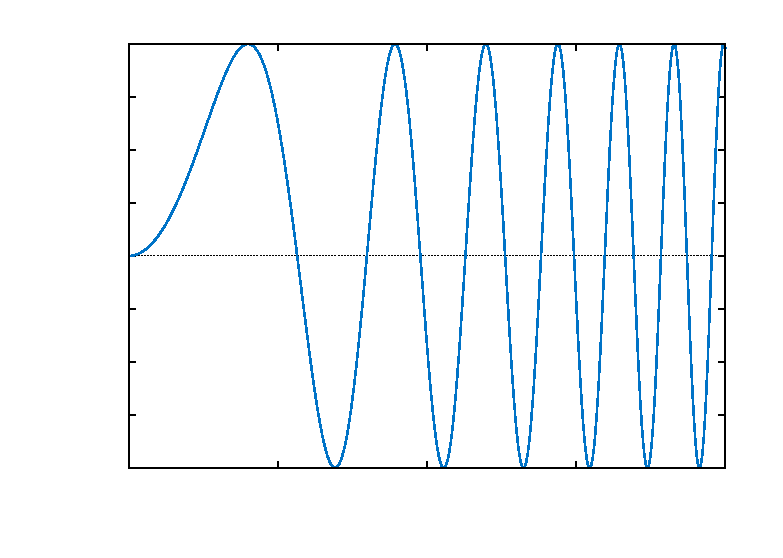
\includegraphics{sinx2}}%
    \gplfronttext
  \end{picture}%
\endgroup
\vspace{-6mm}
 \end{center}
 \caption[]{\quad $y=2\,\sin\;( x^2 )$}
 \label{fig:exmp2sinx2}
\end{figure}

 Notice how the curve ``speeds up'' as $x$ gets larger, making the ``waves'' narrower and narrower.
 Thus, $y=2\,\sin\;( x^2 )$ has no period. Despite this, it appears that the function does have an
 amplitude, namely $2$. To see why, note that since $\abs{\sin\;\theta} \le 1$ for all $\theta$, we
 have
 \begin{displaymath}
  \abs{2\,\sin\;( x^2 )} ~=~ \abs{2} \;\cdot\; \abs{\sin\;( x^2 )} ~\le~ 2 \;\cdot\; 1 ~=~ 2 ~.
 \end{displaymath}
 In the exercises you will be asked to find values of $x$ such that $2\,\sin\;( x^2 )$ reaches the
 maximum value $2$ and the minimum value $-2$. Thus, the amplitude is indeed $2$.\\Note: This curve
 is still sinusoidal despite not being periodic, since the general shape is still that of a ``sine
 wave'', albeit one with variable \emph{cycles}.
\end{exmp}\vspace{-3mm}
\divider
\vspace{1mm}

So far in our examples we have been able to determine the amplitudes of sinusoidal curves fairly
easily. This will not always be the case.
\newpage
\begin{exmp}\label{exmp:3sinx4cosx}
  Find the amplitude and period of $y=3\,\sin\;x + 4\,\cos\;x$.\vspace{1mm}
 \par\noindent\textbf{Solution:} This is sometimes called a \emph{combination} sinusoidal curve, since
 it is the sum of two such curves. The period is still simple to determine: since
 $\sin\;x$ and $\cos\;x$ each repeat every $2\pi$ radians, then so does the combination
 $3\,\sin\;x + 4\,\cos\;x$. Thus, $y=3\,\sin\;x + 4\,\cos\;x$ has period $2\pi$. We can see this in
 the graph, shown in Figure \ref{fig:exmp3sinx4cosx}:\vspace{-1mm}

\begin{figure}[h]
 \begin{center}
  % GNUPLOT: LaTeX picture with Postscript
\begingroup
\footnotesize
  \makeatletter
  \providecommand\color[2][]{%
    \GenericError{(gnuplot) \space\space\space\@spaces}{%
      Package color not loaded in conjunction with
      terminal option `colourtext'%
    }{See the gnuplot documentation for explanation.%
    }{Either use 'blacktext' in gnuplot or load the package
      color.sty in LaTeX.}%
    \renewcommand\color[2][]{}%
  }%
  \providecommand\includegraphics[2][]{%
    \GenericError{(gnuplot) \space\space\space\@spaces}{%
      Package graphicx or graphics not loaded%
    }{See the gnuplot documentation for explanation.%
    }{The gnuplot epslatex terminal needs graphicx.sty or graphics.sty.}%
    \renewcommand\includegraphics[2][]{}%
  }%
  \providecommand\rotatebox[2]{#2}%
  \@ifundefined{ifGPcolor}{%
    \newif\ifGPcolor
    \GPcolortrue
  }{}%
  \@ifundefined{ifGPblacktext}{%
    \newif\ifGPblacktext
    \GPblacktexttrue
  }{}%
  % define a \g@addto@macro without @ in the name:
  \let\gplgaddtomacro\g@addto@macro
  % define empty templates for all commands taking text:
  \gdef\gplbacktext{}%
  \gdef\gplfronttext{}%
  \makeatother
  \ifGPblacktext
    % no textcolor at all
    \def\colorrgb#1{}%
    \def\colorgray#1{}%
  \else
    % gray or color?
    \ifGPcolor
      \def\colorrgb#1{\color[rgb]{#1}}%
      \def\colorgray#1{\color[gray]{#1}}%
      \expandafter\def\csname LTw\endcsname{\color{white}}%
      \expandafter\def\csname LTb\endcsname{\color{black}}%
      \expandafter\def\csname LTa\endcsname{\color{black}}%
      \expandafter\def\csname LT0\endcsname{\color[rgb]{1,0,0}}%
      \expandafter\def\csname LT1\endcsname{\color[rgb]{0,1,0}}%
      \expandafter\def\csname LT2\endcsname{\color[rgb]{0,0,1}}%
      \expandafter\def\csname LT3\endcsname{\color[rgb]{1,0,1}}%
      \expandafter\def\csname LT4\endcsname{\color[rgb]{0,1,1}}%
      \expandafter\def\csname LT5\endcsname{\color[rgb]{1,1,0}}%
      \expandafter\def\csname LT6\endcsname{\color[rgb]{0,0,0}}%
      \expandafter\def\csname LT7\endcsname{\color[rgb]{1,0.3,0}}%
      \expandafter\def\csname LT8\endcsname{\color[rgb]{0.5,0.5,0.5}}%
    \else
      % gray
      \def\colorrgb#1{\color{black}}%
      \def\colorgray#1{\color[gray]{#1}}%
      \expandafter\def\csname LTw\endcsname{\color{white}}%
      \expandafter\def\csname LTb\endcsname{\color{black}}%
      \expandafter\def\csname LTa\endcsname{\color{black}}%
      \expandafter\def\csname LT0\endcsname{\color{black}}%
      \expandafter\def\csname LT1\endcsname{\color{black}}%
      \expandafter\def\csname LT2\endcsname{\color{black}}%
      \expandafter\def\csname LT3\endcsname{\color{black}}%
      \expandafter\def\csname LT4\endcsname{\color{black}}%
      \expandafter\def\csname LT5\endcsname{\color{black}}%
      \expandafter\def\csname LT6\endcsname{\color{black}}%
      \expandafter\def\csname LT7\endcsname{\color{black}}%
      \expandafter\def\csname LT8\endcsname{\color{black}}%
    \fi
  \fi
  \setlength{\unitlength}{0.0500bp}%
  \begin{picture}(7200.00,5040.00)%
    \gplgaddtomacro\gplbacktext{%
      \csname LTb\endcsname%
      \put(682,704){\makebox(0,0)[r]{\strut{}-5}}%
      \csname LTb\endcsname%
      \put(682,1111){\makebox(0,0)[r]{\strut{}-4}}%
      \csname LTb\endcsname%
      \put(682,1518){\makebox(0,0)[r]{\strut{}-3}}%
      \csname LTb\endcsname%
      \put(682,1925){\makebox(0,0)[r]{\strut{}-2}}%
      \csname LTb\endcsname%
      \put(682,2332){\makebox(0,0)[r]{\strut{}-1}}%
      \csname LTb\endcsname%
      \put(682,2740){\makebox(0,0)[r]{\strut{} 0}}%
      \csname LTb\endcsname%
      \put(682,3147){\makebox(0,0)[r]{\strut{} 1}}%
      \csname LTb\endcsname%
      \put(682,3554){\makebox(0,0)[r]{\strut{} 2}}%
      \csname LTb\endcsname%
      \put(682,3961){\makebox(0,0)[r]{\strut{} 3}}%
      \csname LTb\endcsname%
      \put(682,4368){\makebox(0,0)[r]{\strut{} 4}}%
      \csname LTb\endcsname%
      \put(682,4775){\makebox(0,0)[r]{\strut{} 5}}%
      \csname LTb\endcsname%
      \put(814,484){\makebox(0,0){\strut{}$0$}}%
      \csname LTb\endcsname%
      \put(1563,484){\makebox(0,0){\strut{}$\frac{\pi}{2}$}}%
      \csname LTb\endcsname%
      \put(2311,484){\makebox(0,0){\strut{}$\pi$}}%
      \csname LTb\endcsname%
      \put(3060,484){\makebox(0,0){\strut{}$\frac{3\pi}{2}$}}%
      \csname LTb\endcsname%
      \put(3809,484){\makebox(0,0){\strut{}$2\pi$}}%
      \csname LTb\endcsname%
      \put(4557,484){\makebox(0,0){\strut{}$\frac{5\pi}{2}$}}%
      \csname LTb\endcsname%
      \put(5306,484){\makebox(0,0){\strut{}$3\pi$}}%
      \csname LTb\endcsname%
      \put(6054,484){\makebox(0,0){\strut{}$\frac{7\pi}{2}$}}%
      \csname LTb\endcsname%
      \put(6803,484){\makebox(0,0){\strut{}$4\pi$}}%
      \csname LTb\endcsname%
      \put(176,2739){\rotatebox{-270}{\makebox(0,0){\strut{}$y$}}}%
      \put(3808,154){\makebox(0,0){\strut{}$x$}}%
    }%
    \gplgaddtomacro\gplfronttext{%
    }%
    \gplbacktext
    \put(0,0){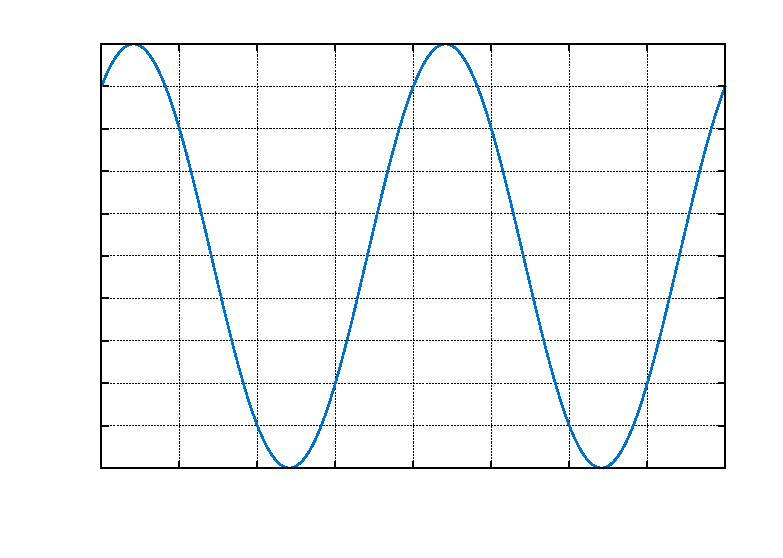
\includegraphics{3sinx4cosx}}%
    \gplfronttext
  \end{picture}%
\endgroup
\vspace{-6mm}
 \end{center}
 \caption[]{\quad $y=3\,\sin\;x + 4\,\cos\;x$}
 \label{fig:exmp3sinx4cosx}
\end{figure}

The graph suggests that the amplitude is $5$, which may not be immediately obvious just by looking at
how the function is defined. In fact, the definition $y=3\,\sin\;x + 4\,\cos\;x$ may tempt you to
think that the amplitude is $7$, since the largest that $3\,\sin\;x$ could be is $3$ and the largest
that $4\,\cos\;x$ could be is $4$, so that the largest their sum could be is $3+4=7$. However,
$3\,\sin\;x$ can never equal $3$ for the same $x$ that makes $4\,\cos\;x$ equal to $4$ (why?).

\piccaption[]{\label{fig:tri345}}\parpic[r]{\begin{tikzpicture}[scale=0.5,
 every node/.style={font=\small}]
 \fill [fill=fillcolor] (0,0) -- (3,0) -- (3,4) -- (0,0);
 \draw (0:1.5) arc (0:53.13:1.5);
 \draw [line width=0.5pt] (2.625,0) -- (2.625,0.375) -- (3,0.375);
 \draw [linecolor,line width=1.5pt] (0,0) -- (3,0) -- (3,4) -- cycle;
 \node [below] at (1.5,0) {$3$};
 \node [right] at (3,2) {$4$};
 \node [above left] at (1.5,2) {$5$};
 \node at (0.9,0.4) {$\theta$};
\end{tikzpicture}}
\picskip{4}
There is a useful technique (which we will discuss further in Chapter 6) for showing that the
amplitude of $y=3\,\sin\;x + 4\,\cos\;x$ is $5$. Let $\theta$ be the angle shown in the right
triangle in Figure \ref{fig:tri345}. Then $\cos\;\theta = \frac{3}{5}$ and $\sin\;\theta =
\frac{4}{5}$. We can use this as follows:
\begin{align*}
 y ~&=~ 3\,\sin\;x ~+~ 4\,\cos\;x\\
 &=~ 5\,\left( \tfrac{3}{5}\,\sin\;x ~+~ \tfrac{4}{5}\,\cos\;x \right)\\
 &=~ 5\,( \cos\;\theta\;\sin\;x ~+~ \sin\;\theta\;\cos\;x )\\
 &=~ 5\,\sin\;(x+\theta)\quad\text{(by the sine addition formula)}
\end{align*}
Thus, $\abs{y} = \abs{5\,\sin\;(x+\theta)} = \abs{5}\,\cdot\,\abs{\sin\;(x+\theta)} \le (5)(1) = 5$,
so the amplitude of $y=3\,\sin\;x + 4\,\cos\;x$ is $5$.
\end{exmp}\vspace{-3mm}
\divider\vspace{-2mm}
\newpage
In general, a combination of sines and cosines will have a period equal to the \emph{lowest common
multiple} of the periods of the sines and cosines being added. In Example \ref{exmp:3sinx4cosx},
$\sin\;x$ and $\cos\;x$ each have period $2\pi$, so the lowest common multiple (which is always an
\emph{integer} multiple) is $1 \,\cdot\, 2\pi = 2\pi$.

\begin{exmp}\label{exmp:cos6xsin4x}
 Find the period of $y=\cos\;6x + \sin\;4x$.\vspace{1mm}
 \par\noindent\textbf{Solution:} The period of $\cos\;6x$ is $\frac{2\pi}{6} = \frac{\pi}{3}$, and the
 period of $\sin\;4x$ is $\frac{2\pi}{4} = \frac{\pi}{2}$. The lowest common multiple of
 $\frac{\pi}{3}$ and $\frac{\pi}{2}$ is $\pi$:
 \begin{alignat*}{4}
  1 \;\cdot\; \tfrac{\pi}{3} ~&=~ \tfrac{\pi}{3} \quad\quad\quad
   &1 \;&\cdot\; \tfrac{\pi}{2} ~&=~ \tfrac{\pi}{2}\\
  2 \;\cdot\; \tfrac{\pi}{3} ~&=~ \tfrac{2\pi}{3} \quad\quad\quad
   &2 \;&\cdot\; \tfrac{\pi}{2} ~&=~ \pi\\
  3 \;\cdot\; \tfrac{\pi}{3} ~&=~ \pi \quad\quad\quad &{} &{}\\
 \end{alignat*}
 Thus, the period of $y=\cos\;6x + \sin\;4x$ is $\pi$. We can see this from its graph in Figure
 \ref{fig:exmpcos6xsin4x}:
 
\begin{figure}[h]
 \begin{center}
  % GNUPLOT: LaTeX picture with Postscript
\begingroup
\footnotesize
  \makeatletter
  \providecommand\color[2][]{%
    \GenericError{(gnuplot) \space\space\space\@spaces}{%
      Package color not loaded in conjunction with
      terminal option `colourtext'%
    }{See the gnuplot documentation for explanation.%
    }{Either use 'blacktext' in gnuplot or load the package
      color.sty in LaTeX.}%
    \renewcommand\color[2][]{}%
  }%
  \providecommand\includegraphics[2][]{%
    \GenericError{(gnuplot) \space\space\space\@spaces}{%
      Package graphicx or graphics not loaded%
    }{See the gnuplot documentation for explanation.%
    }{The gnuplot epslatex terminal needs graphicx.sty or graphics.sty.}%
    \renewcommand\includegraphics[2][]{}%
  }%
  \providecommand\rotatebox[2]{#2}%
  \@ifundefined{ifGPcolor}{%
    \newif\ifGPcolor
    \GPcolortrue
  }{}%
  \@ifundefined{ifGPblacktext}{%
    \newif\ifGPblacktext
    \GPblacktexttrue
  }{}%
  % define a \g@addto@macro without @ in the name:
  \let\gplgaddtomacro\g@addto@macro
  % define empty templates for all commands taking text:
  \gdef\gplbacktext{}%
  \gdef\gplfronttext{}%
  \makeatother
  \ifGPblacktext
    % no textcolor at all
    \def\colorrgb#1{}%
    \def\colorgray#1{}%
  \else
    % gray or color?
    \ifGPcolor
      \def\colorrgb#1{\color[rgb]{#1}}%
      \def\colorgray#1{\color[gray]{#1}}%
      \expandafter\def\csname LTw\endcsname{\color{white}}%
      \expandafter\def\csname LTb\endcsname{\color{black}}%
      \expandafter\def\csname LTa\endcsname{\color{black}}%
      \expandafter\def\csname LT0\endcsname{\color[rgb]{1,0,0}}%
      \expandafter\def\csname LT1\endcsname{\color[rgb]{0,1,0}}%
      \expandafter\def\csname LT2\endcsname{\color[rgb]{0,0,1}}%
      \expandafter\def\csname LT3\endcsname{\color[rgb]{1,0,1}}%
      \expandafter\def\csname LT4\endcsname{\color[rgb]{0,1,1}}%
      \expandafter\def\csname LT5\endcsname{\color[rgb]{1,1,0}}%
      \expandafter\def\csname LT6\endcsname{\color[rgb]{0,0,0}}%
      \expandafter\def\csname LT7\endcsname{\color[rgb]{1,0.3,0}}%
      \expandafter\def\csname LT8\endcsname{\color[rgb]{0.5,0.5,0.5}}%
    \else
      % gray
      \def\colorrgb#1{\color{black}}%
      \def\colorgray#1{\color[gray]{#1}}%
      \expandafter\def\csname LTw\endcsname{\color{white}}%
      \expandafter\def\csname LTb\endcsname{\color{black}}%
      \expandafter\def\csname LTa\endcsname{\color{black}}%
      \expandafter\def\csname LT0\endcsname{\color{black}}%
      \expandafter\def\csname LT1\endcsname{\color{black}}%
      \expandafter\def\csname LT2\endcsname{\color{black}}%
      \expandafter\def\csname LT3\endcsname{\color{black}}%
      \expandafter\def\csname LT4\endcsname{\color{black}}%
      \expandafter\def\csname LT5\endcsname{\color{black}}%
      \expandafter\def\csname LT6\endcsname{\color{black}}%
      \expandafter\def\csname LT7\endcsname{\color{black}}%
      \expandafter\def\csname LT8\endcsname{\color{black}}%
    \fi
  \fi
  \setlength{\unitlength}{0.0500bp}%
  \begin{picture}(7200.00,5040.00)%
    \gplgaddtomacro\gplbacktext{%
      \csname LTb\endcsname%
      \put(946,704){\makebox(0,0)[r]{\strut{}-2}}%
      \csname LTb\endcsname%
      \put(946,1213){\makebox(0,0)[r]{\strut{}-1.5}}%
      \csname LTb\endcsname%
      \put(946,1722){\makebox(0,0)[r]{\strut{}-1}}%
      \csname LTb\endcsname%
      \put(946,2231){\makebox(0,0)[r]{\strut{}-0.5}}%
      \csname LTb\endcsname%
      \put(946,2740){\makebox(0,0)[r]{\strut{} 0}}%
      \csname LTb\endcsname%
      \put(946,3248){\makebox(0,0)[r]{\strut{} 0.5}}%
      \csname LTb\endcsname%
      \put(946,3757){\makebox(0,0)[r]{\strut{} 1}}%
      \csname LTb\endcsname%
      \put(946,4266){\makebox(0,0)[r]{\strut{} 1.5}}%
      \csname LTb\endcsname%
      \put(946,4775){\makebox(0,0)[r]{\strut{} 2}}%
      \csname LTb\endcsname%
      \put(1078,484){\makebox(0,0){\strut{}$0$}}%
      \csname LTb\endcsname%
      \put(2509,484){\makebox(0,0){\strut{}$\frac{\pi}{2}$}}%
      \csname LTb\endcsname%
      \put(3941,484){\makebox(0,0){\strut{}$\pi$}}%
      \csname LTb\endcsname%
      \put(5372,484){\makebox(0,0){\strut{}$\frac{3\pi}{2}$}}%
      \csname LTb\endcsname%
      \put(6803,484){\makebox(0,0){\strut{}$2\pi$}}%
      \put(176,2739){\rotatebox{-270}{\makebox(0,0){\strut{}$y$}}}%
      \put(3940,154){\makebox(0,0){\strut{}$x$}}%
    }%
    \gplgaddtomacro\gplfronttext{%
    }%
    \gplbacktext
    \put(0,0){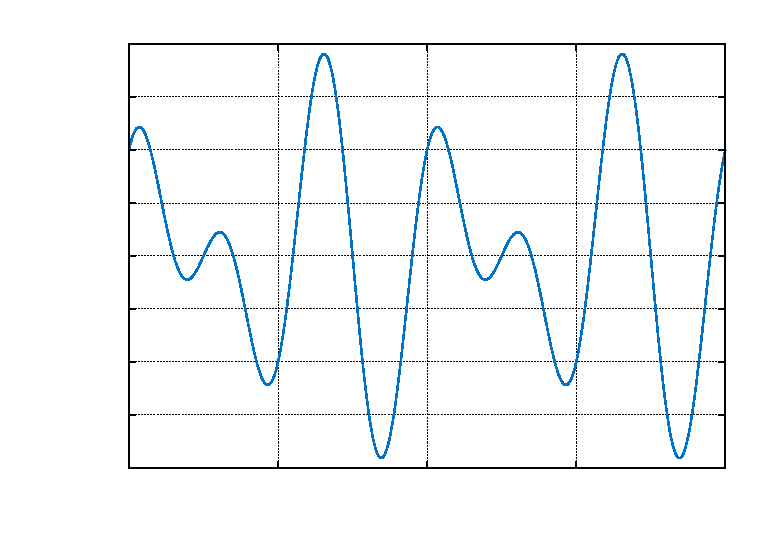
\includegraphics{cos6xsin4x}}%
    \gplfronttext
  \end{picture}%
\endgroup
\vspace{-6mm}
 \end{center}
 \caption[]{\quad $y=\cos\;6x + \sin\;4x$}
 \label{fig:exmpcos6xsin4x}
\end{figure}

 What about the amplitude? Unfortunately we can not use the technique from Example
 \ref{exmp:3sinx4cosx}, since we are not taking the cosine and sine of the same angle; we are
 taking the cosine of $6x$ but the sine of $4x$. In this case, it appears from the graph that the
 maximum is close to $2$ and the minimum is close to $-2$. In Chapter 6, we will describe how to
 use a numerical computation program to show that the maximum and minimum are
 $\pm\,1.90596111871578$, respectively (accurate to within $\approx 2.2204 \times 10^{-16}$). Hence,
 the amplitude is $1.90596111871578$.
\end{exmp}\vspace{-3mm}
\divider\vspace{-2mm}
\newpage
Generalizing Example \ref{exmp:3sinx4cosx}, an expression of the form
$a\,\sin\;\omega x \;+\; b\,\cos\;\omega x$ is equivalent to
$\sqrt{a^2 + b^2}\;\sin\;(x+\theta)$, where $\theta$ is an angle such that
$\cos\;\theta = \frac{a}{\sqrt{a^2 + b^2}}$ and $\sin\;\theta = \frac{b}{\sqrt{a^2 + b^2}}$. So
$y=a\,\sin\;\omega x \;+\; b\,\cos\;\omega x$ will have amplitude $\sqrt{a^2 + b^2}$. Note that this
method only works when the angle $\omega x$ is the same in both the sine and cosine terms.

We have seen how adding a constant to a function shifts the entire graph vertically. We will now see
how to shift the entire graph of a periodic curve horizontally.

\piccaption[]{\enskip $y=A\,\sin\;\omega x$\label{fig:phasenone}}\parpic[r]{\begin{tikzpicture}[scale=1.2,
 every node/.style={font=\small}]
 \begin{scope}[shift={(0,0)},color=linecolor,line width=1.5pt,x=3cm/360]
  \draw[black!60,line width=0.3pt,dotted] (0,-1) grid[xstep=90,ystep=1] (360,1);
  \draw[black!60,line width=0.3pt,-latex] (0,0) -- (380,0) node[right] {$x$};
  \draw[black!60,line width=0.3pt,-latex] (0,-1.2) -- (0,1.6) node[above] {$y$};
  \pgfplothandlerlineto
  \pgfplotfunction{\x}{0,5,...,360}{\pgfpointxy{\x}{sin(\x)}}
  \pgfusepath{stroke}
  \node[black,left] at (0,0) {$0$};
  \foreach \pos in {90,180,270,360}
   \draw[black!60,line width=0.3pt,shift={(\pos,0)}] (0pt,3pt) -- (0pt,-3pt);
  \foreach \pos in {-1,1}
   \draw[black!60,line width=0.3pt,shift={(0,\pos)}] (3pt,0pt) -- (-3pt,0pt);
  \node[black,left] at (0,1) {$A$};
  \node[black,left] at (0,-1) {$-A$};
  \node[black,below] at (180,-0.1) {$\tfrac{\pi}{\omega}$};
  \node[black,below] at (360,-0.1) {$\tfrac{2\pi}{\omega}$};
 \end{scope}
 \begin{scope}[>=latex]
  \draw [<->|] (0,1.3) -- (3,1.3) node[midway,fill=white] {period $= \tfrac{2\pi}{\omega}$};
 \end{scope}
\end{tikzpicture}}
Consider a function of the form $y=A\,\sin\;\omega x$, where $A$ and $\omega$ are nonzero constants.
For simplicity we will assume that $A >0$ and $\omega > 0$ (in general either one could be
negative). Then the amplitude is $A$ and the period is $\frac{2\pi}{\omega}$. The graph is shown in
Figure \ref{fig:phasenone}.

Now consider the function $y=A\,\sin\;(\omega x - \phi)$, where $\phi$ is some constant. The
amplitude is still $A$, and the period is still $\frac{2\pi}{\omega}$, since $\omega x - \phi$ is a
linear function of $x$. Also, we know that the sine function goes through an entire cycle when its
angle goes from $0$ to $2\pi$. Here, we are taking the sine of the angle $\omega x - \phi$. So as
$\omega x - \phi$ goes from $0$ to $2\pi$, an entire cycle of the function
$y=A\,\sin\;(\omega x - \phi)$ will be traced out. That cycle starts when
\begin{align*}
 \omega x - \phi ~=~ 0 \quad&\Rightarrow\quad x ~=~ \frac{\phi}{\omega}\\
\intertext{and ends when}
 \omega x - \phi ~=~ 2\pi \quad&\Rightarrow\quad x ~=~ \frac{2\pi}{\omega}\;+\;\frac{\phi}{\omega}~.
\end{align*}
Thus, the graph of $y=A\,\sin\;(\omega x - \phi)$ is just the graph of $y=A\,\sin\;\omega x$
shifted horizontally by $\frac{\phi}{\omega}$, as in Figure \ref{fig:phaseshift}. The graph is
shifted to the right when $\phi >0$, and to the left when $\phi <0$. The amount
$\frac{\phi}{\omega}$ of the shift is called the \textbf{phase shift}\index{phase shift} of the
graph.

\begin{figure}[h]
 \centering
 \subfloat[][ $\phi >0$: right shift]{
  \begin{tikzpicture}[scale=1.2,every node/.style={font=\small}]
   \begin{scope}[shift={(0,0)},color=linecolor,line width=1.5pt,x=3cm/360]
	\draw[black!60,line width=0.3pt,-latex] (0,0) -- (500,0) node[right] {$x$};
	\draw[black!60,line width=0.3pt,-latex] (0,-1.2) -- (0,1.7) node[above] {$y$};
	\pgfplothandlerlineto
	\pgfplotfunction{\x}{90,95,...,450}{\pgfpointxy{\x}{sin(-90+\x)}}
	\pgfusepath{stroke}
	\node[black,left] at (0,0) {$0$};
	\foreach \pos in {90,180,270,360,450}
	 \draw[black!60,line width=0.3pt,shift={(\pos,0)}] (0pt,3pt) -- (0pt,-3pt);
	\foreach \pos in {-1,1}
	 \draw[black!60,line width=0.3pt,shift={(0,\pos)}] (3pt,0pt) -- (-3pt,0pt);
	\node[black,left] at (0,1) {$A$};
	\node[black,left] at (0,-1) {$-A$};
	\node[black,below right] at (425,-0.1) {$\tfrac{2\pi}{\omega}+\tfrac{\phi}{\omega}$};
	\node[black,below] at (90,-0.1) {$\tfrac{\phi}{\omega}$};
   \end{scope}
   \begin{scope}[>=latex]
    \draw [|<->|] (0.75,1.4) -- (3.75,1.4) node[midway,fill=white]
	 {period $= \tfrac{2\pi}{\omega}$};
    \draw [<->|] (0,-0.9) -- (0.75,-0.9);
	\node[below right] at (0,-0.9) {phase shift};
   \end{scope}
  \end{tikzpicture}}
 \qquad\qquad
 \subfloat[][ $\phi <0$: left shift]{
  \begin{tikzpicture}[scale=1.2,every node/.style={font=\small}]
   \begin{scope}[shift={(0,0)},color=linecolor,line width=1.5pt,x=3cm/360]
	\draw[black!60,line width=0.3pt,-latex] (-120,0) -- (320,0) node[right] {$x$};
	\draw[black!60,line width=0.3pt,-latex] (0,-1.2) -- (0,1.7) node[above] {$y$};
	\pgfplothandlerlineto
	\pgfplotfunction{\x}{-90,-85,...,270}{\pgfpointxy{\x}{sin(90+\x)}}
	\pgfusepath{stroke}
	\node[black,below right] at (0,0) {$0$};
	\foreach \pos in {-90,90,180,270}
	 \draw[black!60,line width=0.3pt,shift={(\pos,0)}] (0pt,3pt) -- (0pt,-3pt);
	\foreach \pos in {-1,1}
	 \draw[black!60,line width=0.3pt,shift={(0,\pos)}] (3pt,0pt) -- (-3pt,0pt);
	\node[black,left] at (0,1.1) {$A$};
	\node[black,right] at (0,-1) {$-A$};
	\node[black,below right] at (245,-0.1) {$\tfrac{2\pi}{\omega}+\tfrac{\phi}{\omega}$};
	\node[black,below] at (-90,-0.1) {$\tfrac{\phi}{\omega}$};
   \end{scope}
   \begin{scope}[>=latex]
    \draw [|<->|] (-0.75,1.4) -- (2.25,1.4) node[pos=0.6,fill=white]
	 {period $= \tfrac{2\pi}{\omega}$};
    \draw [|<->] (-0.75,-0.9) -- (0,-0.9);
	\node[below left] at (0,-0.9) {phase shift};
   \end{scope}
  \end{tikzpicture}}\vspace{-2mm}
 \caption[]{\quad Phase shift for $y=A\,\sin\;(\omega x - \phi)$}
 \label{fig:phaseshift}
\end{figure}
\newpage
The phase shift is defined similarly for the other trigonometric functions.

\begin{exmp}
 Find the amplitude, period, and phase shift of $y=3\,\cos\;(2x - \pi)$.\vspace{1mm}
 \par\noindent\textbf{Solution:} The amplitude is $3$, the period is $\frac{2\pi}{2} = \pi$, and the
 phase shift is $\frac{\pi}{2}$. The graph is shown in Figure \ref{fig:exmp3cos2mpi}:\vspace{-1mm}

\begin{figure}[h]
 \begin{center}
  \begin{tikzpicture}[scale=1.2,every node/.style={font=\small}]
   \begin{scope}[shift={(0,0)},color=linecolor,line width=1.5pt,x=8cm/360,y=1.5cm/3]
    \draw[black!60,line width=0.3pt,dotted] (0,-3) grid[xstep=90,ystep=1] (360,3);
	\draw[black!60,line width=0.3pt,-latex] (0,0) -- (380,0) node[right] {$x$};
	\draw[black!60,line width=0.3pt,-latex] (0,-3.8) -- (0,3.8) node[above] {$y$};
	\pgfplothandlerlineto
	\pgfplotfunction{\x}{0,5,...,360}{\pgfpointxy{\x}{3*cos(-180+2*\x)}}
	\pgfusepath{stroke}
	\node[black,left] at (0,0) {$0$};
	\foreach \pos in {90,180,270,360}
	 \draw[black!60,line width=0.3pt,shift={(\pos,0)}] (0pt,3pt) -- (0pt,-3pt);
	\foreach \pos in {-3,-2,-1,1,2,3}
	 \draw[black!60,line width=0.3pt,shift={(0,\pos)}] (3pt,0pt) -- (-3pt,0pt) node[black,left]
	  {$\pos$};
	\node[black,below] at (90,-0.1) {$\tfrac{\pi}{2}$};
	\node[black,below] at (180,-0.1) {$\pi$};
	\node[black,below] at (270,-0.1) {$\tfrac{3\pi}{2}$};
	\node[black,below] at (360,-0.1) {$2\pi$};
   \end{scope}
   \begin{scope}[>=latex]
    \draw [|<->|] (2,1.9) -- (6,1.9) node[midway,fill=white] {period $= \pi$};
    \draw [<->|] (0,-1.7) -- (2,-1.7);
	\node[below right] at (0,-1.7) {phase shift $= \tfrac{\pi}{2}$};
    \draw [|<->|] (-0.9,0) -- (-0.9,1.5) node[midway,left] {amplitude $= 3$};
   \end{scope}
  \end{tikzpicture}\vspace{-6mm}
 \end{center}
 \caption[]{\quad $y=3\,\cos\;(2x - \pi)$}
 \label{fig:exmp3cos2mpi}
\end{figure}

Notice that the graph is the same as the graph of $y=3\,\cos\;2x$ shifted to the right by
$\frac{\pi}{2}$, the amount of the phase shift.
\end{exmp}
\begin{exmp}
 Find the amplitude, period, and phase shift of $y=-2\,\sin\;\left(3x +
 \frac{\pi}{2}\right)$.\vspace{1mm}
 \par\noindent\textbf{Solution:} The amplitude is $2$, the period is $\frac{2\pi}{3}$, and the
 phase shift is $\frac{-\frac{\pi}{2}}{3} = -\frac{\pi}{6}$. Notice the negative sign in the phase
 shift, since $3x+\pi=3x-(-\pi)$ is in the form $\omega x - \phi$. The graph is shown in Figure
 \ref{fig:exmpm2sin3ppi2}:\vspace{-1mm}

\begin{figure}[h]
 \begin{center}
  \begin{tikzpicture}[scale=1.1,every node/.style={font=\small}]
   \begin{scope}[shift={(0,0)},color=linecolor,line width=1.5pt,x=8cm/240,y=1.5cm/2]
    \draw[black!60,line width=0.3pt,dotted] (-30,-2) grid[xstep=30,ystep=1] (240,2);
	\draw[black!60,line width=0.3pt,-latex] (-50,0) -- (250,0) node[right] {$x$};
	\draw[black!60,line width=0.3pt,-latex] (0,-2.8) -- (0,2.8) node[above] {$y$};
	\pgfplothandlerlineto
	\pgfplotfunction{\x}{-30,-25,...,240}{\pgfpointxy{\x}{-2*sin(90+3*\x)}}
	\pgfusepath{stroke}
	\node[black,below left] at (0,0) {$0$};
	\foreach \pos in {-30,30,60,90,120,150,180,210,240}
	 \draw[black!60,line width=0.3pt,shift={(\pos,0)}] (0pt,3pt) -- (0pt,-3pt);
	\foreach \pos in {-2,-1,1,2}
	 \draw[black!60,line width=0.3pt,shift={(0,\pos)}] (3pt,0pt) -- (-3pt,0pt) node[black,left]
	  {$\pos$};
	\node[black,below] at (-35,-0.1) {$-\tfrac{\pi}{6}$};
	\node[black,below] at (30,-0.1) {$\tfrac{\pi}{6}$};
	\node[black,below] at (60,-0.1) {$\tfrac{\pi}{3}$};
	\node[black,below] at (90,-0.1) {$\tfrac{\pi}{2}$};
	\node[black,below] at (120,-0.1) {$\tfrac{2\pi}{3}$};
	\node[black,below] at (150,-0.1) {$\tfrac{5\pi}{6}$};
	\node[black,below] at (180,-0.1) {$\pi$};
	\node[black,below] at (210,-0.1) {$\tfrac{7\pi}{6}$};
	\node[black,below] at (240,-0.1) {$\tfrac{4\pi}{3}$};
   \end{scope}
   \begin{scope}[>=latex]
    \draw [|<->|] (-1,1.9) -- (3,1.9) node[pos=0.55,fill=white] {period $= \frac{2\pi}{3}$};
    \draw [|<->] (-1,-1.7) -- (0,-1.7);
	\node[below left] at (0,-1.75) {phase shift $= -\tfrac{\pi}{6}$};
    \draw [|<->|] (-1.1,0) -- (-1.1,1.5) node[midway,left] {amplitude $= 2$};
   \end{scope}
  \end{tikzpicture}\vspace{-6mm}
 \end{center}
 \caption[]{\quad $y=-2\,\sin\;\left( 3x + \frac{\pi}{2} \right)$}
 \label{fig:exmpm2sin3ppi2}
\end{figure}
\end{exmp}\vspace{-4mm}
\divider\vspace{-2mm}
\newpage
In engineering two periodic functions with the same period are said to be \emph{out of
phase} if their phase shifts differ. For example, $\sin\;\left( x -
\frac{\pi}{6} \right)$ and $\sin\;x$ would be $\frac{\pi}{6}$ radians (or $30\Degrees$) out of
phase, and $\sin\;x$ would be said to \emph{lag} $\sin\;\left( x - \frac{\pi}{6} \right)$ by
$\frac{\pi}{6}$ radians, while $\sin\;\left( x - \frac{\pi}{6} \right)$ \emph{leads}
$\sin\;x$ by $\frac{\pi}{6}$ radians. Periodic functions with the same period and the same phase
shift are \emph{in phase}.\index{phase, out of or in}

The following is a summary of the properties of trigonometric graphs:

\begin{center}\statecomment{For any constants $A \ne 0$, $\omega \ne 0$, and $\phi$:
\begin{align*}
 y = A\,\sin\;(\omega x - \phi) ~~&\text{has amplitude $\abs{A}$, period $\tfrac{2\pi}{\omega}$, and
  phase shift $\tfrac{\phi}{\omega}$}\\
 y = A\,\cos\;(\omega x - \phi) ~~&\text{has amplitude $\abs{A}$, period $\tfrac{2\pi}{\omega}$, and
  phase shift $\tfrac{\phi}{\omega}$}\\
 y = A\,\tan\;(\omega x - \phi) ~~&\text{has undefined amplitude, period $\tfrac{\pi}{\omega}$, and
  phase shift $\tfrac{\phi}{\omega}$}\\
 y = A\,\csc\;(\omega x - \phi) ~~&\text{has undefined amplitude, period $\tfrac{2\pi}{\omega}$, and
  phase shift $\tfrac{\phi}{\omega}$}\\
 y = A\,\sec\;(\omega x - \phi) ~~&\text{has undefined amplitude, period $\tfrac{2\pi}{\omega}$, and
  phase shift $\tfrac{\phi}{\omega}$}\\
 y = A\,\cot\;(\omega x - \phi) ~~&\text{has undefined amplitude, period $\tfrac{\pi}{\omega}$, and
  phase shift $\tfrac{\phi}{\omega}$}
\end{align*}}\end{center}\vspace{-4mm}

\divider
\vspace{2mm}

\startexercises\label{sec5dot2}
\vspace{5mm}
{\small
\par\noindent For Exercises 1-12, find the amplitude, period, and phase shift of the given function.
Then graph one cycle of the function, either by hand or by using Gnuplot (see Appendix B).
\begin{enumerate}[\bfseries 1.]
\begin{multicols}{4}
 \item $y=3\,\cos\;\pi x$
 \item $y=\sin\;(2\pi x - \pi)$
 \item $y=-\sin\;(5x + 3)$
 \item $y=1+8\,\cos\;(6x- \pi)$
\end{multicols}
\begin{multicols}{4}
 \item $y=2+\cos\;(5x + \pi)$
 \item $y=1-\sin\;(3\pi - 2x)$
 \item $y=1-\cos\;(3\pi - 2x)$
 \item $y=2\,\tan\;(x - 1)$
\end{multicols}
\begin{multicols}{4}
 \item $y=1-\tan\;(3\pi - 2x)$
 \item $y=\sec\;(2x + 1)$
 \item $y=2\csc\;(2x - 1)$
 \item $y=2+4\,\cot\;(1-x)$
\end{multicols}
 \item For the function $y=2\,\sin\;( x^2 )$ in Example \ref{exmp:2sinx2}, for which values of $x$
  does the function reach its maximum value $2$, and for which values of $x$ does it reach
  its minimum value $-2\,$?
 \item For the function $y=3\,\sin\;x + 4\,\cos\;x$ in Example \ref{exmp:3sinx4cosx}, for which
  values of $x$ does the function reach its maximum value $5$, and for which values of $x$ does it
  reach its minimum value $-5\,$? You can restrict your answers to be between $0$ and $2\pi$.
 \item Graph the function $y=\sin^2 \,x$ from $x=0$ to $x=2\pi$, either by hand or by using Gnuplot.
  What are the amplitude and period of this function?
 \item\label{exer:circuitphase}
  The current $i(t)$ in an AC electrical circuit at time $t\ge 0$ is given by
  $i(t) = I_m \,\sin\;\omega t$, and the voltage $v(t)$ is given by $v(t) = V_m \,\sin\;\omega t$,
  where $V_m > I_m > 0$ and $\omega > 0$ are constants.
  Sketch one cycle of both $i(t)$ and $v(t)$ \emph{together on the same graph} (i.e. on the same set
  of axes). Are the current and voltage in phase or out of phase?
 \item Repeat Exercise \ref{exer:circuitphase} with $i(t)$ the same as before but with $v(t)=
  V_m \,\sin\;\left(\omega t + \frac{\pi}{4}\right)$.
 \item Repeat Exercise \ref{exer:circuitphase} with
  $i(t)=-I_m \,\cos\;\left(\omega t - \frac{\pi}{3}\right)$ and $v(t)=
  V_m \,\sin\;\left(\omega t - \frac{5\pi}{6}\right)$.
\suspend{enumerate}
 For Exercises \ref{exer:ampcombostart}-\ref{exer:ampcomboend}, find the amplitude and period of
 the given function. Then graph one cycle of the function, either by hand or by using Gnuplot.
\resume{enumerate}[{[\bfseries 1.]}]
\begin{multicols}{3}
 \item\label{exer:ampcombostart} $y=3\,\sin\;\pi x \;-\; 5\,\cos\;\pi x$
 \item $y=-5\,\sin\;3x \;+\; 12\,\cos\;3x$
 \item\label{exer:ampcomboend} $y=2\,\cos\;x \;+\; 2\,\sin\;x$
\end{multicols}
 \item Find the amplitude of the function $y=2\,\sin\;( x^2 ) \;+\; \cos\;( x^2 )$.
\suspend{enumerate}
 For Exercises \ref{exer:percombostart}-\ref{exer:percomboend}, find the period of the given
 function. Graph one cycle using Gnuplot.
\resume{enumerate}[{[\bfseries 1.]}]
\begin{multicols}{3}
 \item\label{exer:percombostart} $y=\sin\;3x \;-\; \cos\;5x$
 \item $y=\sin\;\frac{x}{3} \;+\; 2\,\cos\;\frac{3x}{4}$
 \item\label{exer:percomboend} $y=2\,\sin\;\pi x \;+\; 3\,\cos\;\frac{\pi}{3}x$
\end{multicols}
 \item Let $y = 0.5\,\sin\;x ~\sin\;12x\,$. Its graph for $x$ from $0$ to $4\pi$ is shown in
  Figure \ref{fig:modulated}:

\begin{figure}[h]
 \begin{center}
  % GNUPLOT: LaTeX picture with Postscript
\begingroup
\footnotesize
  \makeatletter
  \providecommand\color[2][]{%
    \GenericError{(gnuplot) \space\space\space\@spaces}{%
      Package color not loaded in conjunction with
      terminal option `colourtext'%
    }{See the gnuplot documentation for explanation.%
    }{Either use 'blacktext' in gnuplot or load the package
      color.sty in LaTeX.}%
    \renewcommand\color[2][]{}%
  }%
  \providecommand\includegraphics[2][]{%
    \GenericError{(gnuplot) \space\space\space\@spaces}{%
      Package graphicx or graphics not loaded%
    }{See the gnuplot documentation for explanation.%
    }{The gnuplot epslatex terminal needs graphicx.sty or graphics.sty.}%
    \renewcommand\includegraphics[2][]{}%
  }%
  \providecommand\rotatebox[2]{#2}%
  \@ifundefined{ifGPcolor}{%
    \newif\ifGPcolor
    \GPcolortrue
  }{}%
  \@ifundefined{ifGPblacktext}{%
    \newif\ifGPblacktext
    \GPblacktexttrue
  }{}%
  % define a \g@addto@macro without @ in the name:
  \let\gplgaddtomacro\g@addto@macro
  % define empty templates for all commands taking text:
  \gdef\gplbacktext{}%
  \gdef\gplfronttext{}%
  \makeatother
  \ifGPblacktext
    % no textcolor at all
    \def\colorrgb#1{}%
    \def\colorgray#1{}%
  \else
    % gray or color?
    \ifGPcolor
      \def\colorrgb#1{\color[rgb]{#1}}%
      \def\colorgray#1{\color[gray]{#1}}%
      \expandafter\def\csname LTw\endcsname{\color{white}}%
      \expandafter\def\csname LTb\endcsname{\color{black}}%
      \expandafter\def\csname LTa\endcsname{\color{black}}%
      \expandafter\def\csname LT0\endcsname{\color[rgb]{1,0,0}}%
      \expandafter\def\csname LT1\endcsname{\color[rgb]{0,1,0}}%
      \expandafter\def\csname LT2\endcsname{\color[rgb]{0,0,1}}%
      \expandafter\def\csname LT3\endcsname{\color[rgb]{1,0,1}}%
      \expandafter\def\csname LT4\endcsname{\color[rgb]{0,1,1}}%
      \expandafter\def\csname LT5\endcsname{\color[rgb]{1,1,0}}%
      \expandafter\def\csname LT6\endcsname{\color[rgb]{0,0,0}}%
      \expandafter\def\csname LT7\endcsname{\color[rgb]{1,0.3,0}}%
      \expandafter\def\csname LT8\endcsname{\color[rgb]{0.5,0.5,0.5}}%
    \else
      % gray
      \def\colorrgb#1{\color{black}}%
      \def\colorgray#1{\color[gray]{#1}}%
      \expandafter\def\csname LTw\endcsname{\color{white}}%
      \expandafter\def\csname LTb\endcsname{\color{black}}%
      \expandafter\def\csname LTa\endcsname{\color{black}}%
      \expandafter\def\csname LT0\endcsname{\color{black}}%
      \expandafter\def\csname LT1\endcsname{\color{black}}%
      \expandafter\def\csname LT2\endcsname{\color{black}}%
      \expandafter\def\csname LT3\endcsname{\color{black}}%
      \expandafter\def\csname LT4\endcsname{\color{black}}%
      \expandafter\def\csname LT5\endcsname{\color{black}}%
      \expandafter\def\csname LT6\endcsname{\color{black}}%
      \expandafter\def\csname LT7\endcsname{\color{black}}%
      \expandafter\def\csname LT8\endcsname{\color{black}}%
    \fi
  \fi
  \setlength{\unitlength}{0.0500bp}%
  \begin{picture}(7200.00,5040.00)%
    \gplgaddtomacro\gplbacktext{%
      \csname LTb\endcsname%
      \put(946,704){\makebox(0,0)[r]{\strut{}-1}}%
      \put(946,1722){\makebox(0,0)[r]{\strut{}-0.5}}%
      \put(946,2740){\makebox(0,0)[r]{\strut{} 0}}%
      \put(946,3757){\makebox(0,0)[r]{\strut{} 0.5}}%
      \put(946,4775){\makebox(0,0)[r]{\strut{} 1}}%
      \put(1078,484){\makebox(0,0){\strut{}$0$}}%
      \put(2509,484){\makebox(0,0){\strut{}$\pi$}}%
      \put(3941,484){\makebox(0,0){\strut{}$2\pi$}}%
      \put(5372,484){\makebox(0,0){\strut{}$3\pi$}}%
      \put(6803,484){\makebox(0,0){\strut{}$4\pi$}}%
      \csname LTb\endcsname%
      \put(176,2739){\rotatebox{-270}{\makebox(0,0){\strut{}$y$}}}%
      \put(3940,154){\makebox(0,0){\strut{}$x$}}%
    }%
    \gplgaddtomacro\gplfronttext{%
      \csname LTb\endcsname%
      \put(5816,4602){\makebox(0,0)[r]{\strut{}$0.5*\sin(x)*\sin(12*x)$}}%
      \csname LTb\endcsname%
      \put(5816,4382){\makebox(0,0)[r]{\strut{}$0.5*\sin(x)$}}%
      \csname LTb\endcsname%
      \put(5816,4162){\makebox(0,0)[r]{\strut{}$-0.5*\sin(x)$}}%
    }%
    \gplbacktext
    \put(0,0){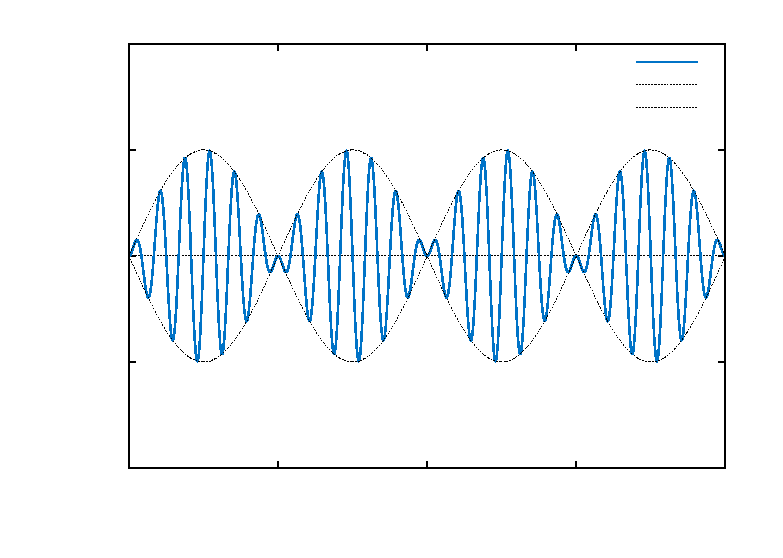
\includegraphics{modulated}}%
    \gplfronttext
  \end{picture}%
\endgroup
\vspace{-6mm}
 \end{center}
 \caption[]{\quad Modulated wave $y=0.5\,\sin\;x ~\sin\;12x$}
 \label{fig:modulated}
\end{figure}

  You can think of this function as $\sin\;12x$ with a sinusoidally varying ``amplitude''of
  $0.5\,\sin\;x$. What is the period of this function?
  From the graph it looks like the amplitude may be $0.5$.
  Without finding the exact amplitude, explain why the amplitude is in fact \emph{less} than $0.5$.
  The function above is known as a \emph{modulated wave}\index{modulated wave}, and the functions
  $\pm\,0.5\,\sin\;x$ form an \emph{amplitude envelope}\index{amplitude envelope} for the wave (i.e.
  they enclose the wave). Use an identity from Section 3.4 to write this function as a sum of
  sinusoidal curves.
 \item Use Gnuplot to graph the function $y= x^2 \,\sin\;10x$ from $x = -2\pi$ to $x=2\pi$. What
  functions form its amplitude envelope? (Note: Use \texttt{set samples 500} in Gnuplot.)
 \item Use Gnuplot to graph the function $y= \frac{1}{x^2} \,\sin\;80x$ from $x = 0.2$ to $x=\pi$.
  What functions form its amplitude envelope? (Note: Use \texttt{set samples 500} in Gnuplot.)
 \item Does the function $y=\sin\;\pi x \;+\; \cos\;x$ have a period? Explain your answer.
 \item Use Gnuplot to graph the function $y=\frac{\sin\;x}{x}$ from $x=-4\pi$ to $x=4\pi$. What
  happens at $x=0$?
\end{enumerate}}
\newpage
%Begin Section 5.3
\section{Inverse Trigonometric Functions}
We have briefly mentioned the inverse trigonometric functions before, for example in Section 1.3
when we discussed how to use the {\setlength\fboxsep{1pt}\ovalbox{\footnotesize $\sin^{-1}$}},
{\setlength\fboxsep{1pt}\ovalbox{\footnotesize $\cos^{-1}$}}, and
{\setlength\fboxsep{1pt}\ovalbox{\footnotesize $\tan^{-1}$}} buttons on a calculator to find
an angle that has a certain trigonometric function value. We will now define those inverse
functions and determine their graphs.\index{inverse trigonometric functions}

\piccaption[]{\label{fig:function}}\parpic[r]{\begin{tikzpicture}[every node/.style={font=\small}]
 \draw [line width=1pt] (0,0) ellipse (0.8 and 0.5);
 \fill (0,0) circle (2pt);
 \node [below] at (0,0) {$x$};
 \node [above] at (0,0.6) {Domain};
 \draw [line width=1pt] (3,0) ellipse (0.8 and 0.5);
 \fill (3,0) circle (2pt);
 \node [below] at (3,0) {$y$};
 \node [above] at (3,0.53) {Range};
 \draw [-latex,line width=1.5pt] (1,0) -- (2,0) node[midway,above] {$f$}
  node[midway,below] {$y=f(x)$};
\end{tikzpicture}}
Recall that a \textbf{function}\index{function} is a rule that assigns a single object $y$ from one
set (the \textbf{range})\index{range} to each object $x$ from another set (the
\textbf{domain}).\index{domain} We can write that rule as $y = f(x)$, where $f$ is the function (see
Figure \ref{fig:function}). There is a simple \emph{vertical rule} for determining whether a rule
$y=f(x)$ is a function: $f$ is a function if and only if every vertical line intersects the graph of
$y=f(x)$ in the $xy$-coordinate plane at most once (see  Figure \ref{fig:verticalrule}).

\begin{figure}[h]
 \centering
 \subfloat[][ $f$ is a function]{
  \begin{tikzpicture}[every node/.style={font=\small}]
   \draw[latex-latex,black!60,line width=0.3pt] (0,2) node[above] {$y$} |- (4,0) node[right] {$x$};
   \draw [linecolor,line width=1.5pt] (0.5,0.5) parabola[bend at end] (3.5,1.5);
   \node[above] at (3.5,1.5) {$y=f(x)$};
   \draw (1.5,0.5) -- (1.5,2);
  \end{tikzpicture}}
 \qquad\qquad
 \subfloat[][ $f$ is not a function]{
  \begin{tikzpicture}[every node/.style={font=\small}]
   \draw[latex-latex,black!60,line width=0.3pt] (0,2) node[above] {$y$} |- (4,0) node[right] {$x$};
   \draw [linecolor,line width=1.5pt] (0.5,1.5) parabola bend  (3.5,1) (2.5,0.5);
   \node[above] at (1.5,1.5) {$y=f(x)$};
   \draw (2.8,0.2) -- (2.8,2);
  \end{tikzpicture}}\vspace{-2mm}
 \caption[]{\quad Vertical rule for functions}
 \label{fig:verticalrule}
\end{figure}

Recall that a function $f$ is \textbf{one-to-one}\index{one-to-one} (often written as $1-1$) if
it assigns distinct values of $y$ to distinct values of $x$. In other words, if $x_1 \ne x_2$ then
$f(x_1 ) \ne f(x_2 )$. Equivalently, $f$ is one-to-one if $f(x_1 ) = f(x_2 )$ implies $x_1 = x_2$.
There is a simple \emph{horizontal rule} for determining whether a function $y=f(x)$ is one-to-one:
$f$ is one-to-one if and only if every horizontal line intersects the graph of $y=f(x)$ in the
$xy$-coordinate plane at most once (see Figure \ref{fig:horizontalrule}).

\begin{figure}[h]
 \centering
 \subfloat[][ $f$ is one-to-one]{
  \begin{tikzpicture}[every node/.style={font=\small}]
   \draw[latex-latex,black!60,line width=0.3pt] (0,2) node[above] {$y$} |- (4,0) node[right] {$x$};
   \draw [linecolor,line width=1.5pt] (0.5,0.5) parabola[bend at end] (3.5,1.5);
   \node[above] at (3.5,1.5) {$y=f(x)$};
   \draw (0.5,1) -- (2.5,1);
  \end{tikzpicture}}
 \qquad\qquad
 \subfloat[][ $f$ is not one-to-one]{
  \begin{tikzpicture}[every node/.style={font=\small}]
   \draw[latex-latex,black!60,line width=0.3pt] (0,2) node[above] {$y$} |- (4,0) node[right] {$x$};
   \draw [linecolor,line width=1.5pt] (0.5,0.5) parabola bend  (2,1.5) (3.5,0.5);
   \node[above] at (2,1.5) {$y=f(x)$};
   \draw (0.5,1) -- (3.5,1);
  \end{tikzpicture}}\vspace{-2mm}
 \caption[]{\quad Horizontal rule for one-to-one functions}
 \label{fig:horizontalrule}
\end{figure}

If a function $f$ is one-to-one on its domain, then $f$ has an \textbf{inverse function}, denoted
by $f^{-1}$, such that $y=f(x)$ if and only if $f^{-1}(y) = x$. The domain of $f^{-1}$ is the
range of $f$.

The basic idea is that $f^{-1}$ ``undoes'' what $f$ does, and vice versa. In other words,
\begin{alignat*}{3}
 f^{-1}(f(x)) ~&=~ x \quad&&\text{for all $x$ in the domain of $f$, and}\\
 f(f^{-1}(y)) ~&=~ y \quad&&\text{for all $y$ in the range of $f$.}
\end{alignat*}

We know from their graphs that none of the trigonometric functions are one-to-one over their entire
domains. However, we can restrict those functions to \emph{subsets} of their domains where they
\emph{are} one-to-one. For example, $y=\sin\;x$ is one-to-one over the interval
$\left[ -\frac{\pi}{2},\frac{\pi}{2} \right]$, as we see in the graph below:

\begin{figure}[h]
 \begin{center}
  \begin{tikzpicture}[scale=1.2,every node/.style={font=\small}]
   \begin{scope}[dashed,line width=1pt,x=6cm/360]
	\draw[black!60,solid,line width=0.3pt,-latex] (-200,0) -- (220,0) node[right] {$x$};
	\draw[black!60,solid,line width=0.3pt,-latex] (0,-1.5) -- (0,1.5) node[above] {$y$};
	\pgfplothandlerlineto
	\pgfplotfunction{\x}{-180,-175,...,180}{\pgfpointxy{\x}{sin(\x)}}
	\pgfusepath{stroke}
	\node[black,below right] at (0,0) {$0$};
	\foreach \pos in {-180,-90,90,180}
	 \draw[black!60,line width=0.3pt,solid,shift={(\pos,0)}] (0pt,3pt) -- (0pt,-3pt);
	\foreach \pos in {-1,1}
	 \draw[black!60,line width=0.3pt,solid,shift={(0,\pos)}] (3pt,0pt) -- (-3pt,0pt)
	  node[black,left] {$\pos$};
	\node[black,below] at (90,-0.1) {$\tfrac{\pi}{2}$};
	\node[black,below] at (180,-0.1) {$\pi$};
	\node[black,below] at (-90,-0.1) {$-\tfrac{\pi}{2}$};
	\node[black,below] at (-180,-0.1) {$-\pi$};
	\node[black,above] at (180,1) {$y=\sin\;x$};
   \end{scope}
   \begin{scope}[color=linecolor,line width=1.5pt,x=6cm/360]
	\pgfplothandlerlineto
	\pgfplotfunction{\x}{-90,-85,...,90}{\pgfpointxy{\x}{sin(\x)}}
	\pgfusepath{stroke}
	\fill (-90,-1) circle (2pt);
	\fill (90,1) circle (2pt);
   \end{scope}
  \end{tikzpicture}\vspace{-6mm}
 \end{center}
 \caption[]{\quad $y=\sin\;x$ with $x$ restricted to $\left[ -\frac{\pi}{2},\frac{\pi}{2} \right]$}
 \label{fig:sinerestricted}
\end{figure}

For $-\frac{\pi}{2} \le x \le \frac{\pi}{2}$ we have $-1 \le \sin\;x \le 1$, so we can define the
\textbf{inverse sine}\index{inverse sine} function $y=\sin^{-1} x$ (sometimes called the \textbf{arc
sine}\index{arc sine} and denoted by $y=\arcsin\;x$) whose domain is the interval $\ival{-1}{1}$ and
whose range is the interval $\left[ -\frac{\pi}{2},\frac{\pi}{2} \right]$. In other words:

\begin{center}\statecomment{\vspace{-4mm}\begin{alignat}{3}
 \sin^{-1} (\sin\;y) ~&=~ y \quad&&\text{for $-\tfrac{\pi}{2} \le y \le
  \tfrac{\pi}{2}$}\label{eqn:arcsin1}\\
 \sin\;(\sin^{-1} x) ~&=~ x \quad&&\text{for $-1 \le x \le 1$}\label{eqn:arcsin2}
\end{alignat}}\end{center}

\begin{exmp}
 Find $\sin^{-1} \left(\sin\;\frac{\pi}{4}\right)$.\vspace{1mm}
 \par\noindent\textbf{Solution:} Since $-\frac{\pi}{2} \le \frac{\pi}{4} \le \frac{\pi}{2}$, we know
 that $\sin^{-1} \left(\sin\;\frac{\pi}{4}\right) = \boxed{\frac{\pi}{4}}\;$, by formula
 (\ref{eqn:arcsin1}).
\end{exmp}
\begin{exmp}\label{exmp:arcsin5pi4}
 Find $\sin^{-1} \left(\sin\;\frac{5\pi}{4}\right)$.\vspace{1mm}
 \par\noindent\textbf{Solution:} Since $\frac{5\pi}{4} > \frac{\pi}{2}$, we can not use formula
 (\ref{eqn:arcsin1}). But we know that $\sin\;\frac{5\pi}{4} = -\frac{1}{\sqrt{2}}$. Thus,
 $\sin^{-1} \left(\sin\;\frac{5\pi}{4}\right) = \sin^{-1} \left( -\frac{1}{\sqrt{2}} \right)$ is, by
 definition, the angle $y$ such that $-\frac{\pi}{2} \le y \le \frac{\pi}{2}$ and $\sin\;y =
 -\frac{1}{\sqrt{2}}$. That angle is $y=-\frac{\pi}{4}$, since
 \begin{displaymath}
  \sin\;\left( -\tfrac{\pi}{4} \right) ~=~ -\sin\;\left( \tfrac{\pi}{4} \right) ~=~
  -\tfrac{1}{\sqrt{2}} ~.
 \end{displaymath}
 Thus, $\sin^{-1} \left(\sin\;\frac{5\pi}{4}\right) = \boxed{-\tfrac{\pi}{4}}\;$.
\end{exmp}
\divider
\newpage
Example \ref{exmp:arcsin5pi4} illustrates an important point: $\sin^{-1} x$ should \emph{always}
be a number between $-\frac{\pi}{2}$ and $\frac{\pi}{2}$. If you get a number outside that range,
then you made a mistake somewhere. This why in Example \ref{exmp:sinneg0682} in Section 1.5 we got
$\sin^{-1}(-0.682) = -43\Degrees$ when using the
{\setlength\fboxsep{1pt}\ovalbox{\footnotesize $\sin^{-1}$}} button on a calculator. Instead of
an angle between $0\Degrees$ and $360\Degrees$ (i.e. $0$ to $2\pi$ radians) we got an angle
between $-90\Degrees$ and $90\Degrees$ (i.e. $-\frac{\pi}{2}$ to $\frac{\pi}{2}$ radians).

In general, the graph of an inverse function $f^{-1}$ is the reflection of the graph of $f$ around
the line $y=x$. The graph of $y=\sin^{-1} x$ is shown in Figure \ref{fig:arcsine}. Notice the
symmetry about the line $y=x$ with the graph of $y=\sin\;x$.

\begin{figure}[h]
 \begin{center}
  \begin{tikzpicture}[scale=1.2,every node/.style={font=\small}]
   \begin{scope}[dashed,line width=1pt,x=6cm/360]
	\draw[black!60,solid,line width=0.3pt,-latex] (-110,0) -- (110,0) node[right] {$x$};
	\draw[black!60,solid,line width=0.3pt,-latex] (0,-2) -- (0,2) node[above] {$y$};
	\pgfplothandlerlineto
	\pgfplotfunction{\x}{-90,-85,...,90}{\pgfpointxy{\x}{sin(\x)}}
	\pgfusepath{stroke}
	\node[black,below right] at (0,0) {$0$};
	\foreach \pos in {-90,-57.3,57.3,90}
	 \draw[black!60,line width=0.3pt,solid,shift={(\pos,0)}] (0pt,3pt) -- (0pt,-3pt);
	\foreach \pos in {-1,1}
	 \draw[black!60,line width=0.3pt,solid,shift={(0,\pos)}] (3pt,0pt) -- (-3pt,0pt)
	  node[black,left] {$\pos$};
	\foreach \pos in {-1.57}
	 \draw[black!60,line width=0.3pt,solid,shift={(0,\pos)}] (3pt,0pt) -- (-3pt,0pt)
	  node[black,left] {$-\tfrac{\pi}{2}$};
	\foreach \pos in {1.57}
	 \draw[black!60,line width=0.3pt,solid,shift={(0,\pos)}] (3pt,0pt) -- (-3pt,0pt)
	  node[black,left] {$\tfrac{\pi}{2}$};
	\node[black,below] at (90,-0.1) {$\tfrac{\pi}{2}$};
	\node[black,below] at (57.3,-0.1) {$1$};
	\node[black,below] at (-90,-0.1) {$-\tfrac{\pi}{2}$};
	\node[black,below] at (-57.3,-0.1) {$-1$};
	\node[linecolor,above] at (57.3,1.58) {$y=\sin^{-1} x$};
	\node[black,right] at (90,1) {$y=\sin\;x$};
	\draw[black!60] (-90,-1.57) -- (90,1.57) node[pos=0.0,left] {$y=x$};
   \end{scope}
   \begin{scope}[color=linecolor,line width=1.5pt,x=6cm/360,cm={0,1,1,0,(0,0)}]
	\pgfplothandlerlineto
	\pgfplotfunction{\x}{-90,-85,...,90}{\pgfpointxy{\x}{sin(\x)}}
	\pgfusepath{stroke}
	\fill (-90,-1) circle (2pt);
	\fill (90,1) circle (2pt);
   \end{scope}
  \end{tikzpicture}\vspace{-6mm}
 \end{center}
 \caption[]{\quad Graph of $y=\sin^{-1} x$}
 \label{fig:arcsine}
\end{figure}

The \textbf{inverse cosine}\index{inverse cosine} function $y=\cos^{-1} x$ (sometimes called the
\textbf{arc cosine}\index{arc cosine} and denoted by $y=\arccos\;x$) can be determined in a similar
fashion. The function $y=\cos\;x$ is one-to-one over the interval $\ival{0}{\pi}$, as we see in the
graph below:

\begin{figure}[h]
 \begin{center}
  \begin{tikzpicture}[scale=1.2,every node/.style={font=\small}]
   \begin{scope}[dashed,line width=1pt,x=6cm/360]
	\draw[black!60,solid,line width=0.3pt,-latex] (-110,0) -- (290,0) node[right] {$x$};
	\draw[black!60,solid,line width=0.3pt,-latex] (0,-1.5) -- (0,1.5) node[above] {$y$};
	\pgfplothandlerlineto
	\pgfplotfunction{\x}{-90,-85,...,270}{\pgfpointxy{\x}{cos(\x)}}
	\pgfusepath{stroke}
	\node[black,below right] at (0,0) {$0$};
	\foreach \pos in {-90,90,180,270}
	 \draw[black!60,line width=0.3pt,solid,shift={(\pos,0)}] (0pt,3pt) -- (0pt,-3pt);
	\foreach \pos in {-1,1}
	 \draw[black!60,line width=0.3pt,solid,shift={(0,\pos)}] (3pt,0pt) -- (-3pt,0pt)
	  node[black,left] {$\pos$};
	\node[black,below] at (90,-0.1) {$\tfrac{\pi}{2}$};
	\node[black,below] at (180,-0.1) {$\pi$};
	\node[black,below] at (-90,-0.1) {$-\tfrac{\pi}{2}$};
	\node[black,below] at (270,-0.1) {$\tfrac{3\pi}{2}$};
	\node[black,above] at (90,1) {$y=\cos\;x$};
   \end{scope}
   \begin{scope}[color=linecolor,line width=1.5pt,x=6cm/360]
	\pgfplothandlerlineto
	\pgfplotfunction{\x}{0,5,...,180}{\pgfpointxy{\x}{cos(\x)}}
	\pgfusepath{stroke}
	\fill (0,1) circle (2pt);
	\fill (180,-1) circle (2pt);
   \end{scope}
  \end{tikzpicture}\vspace{-6mm}
 \end{center}
 \caption[]{\quad $y=\cos\;x$ with $x$ restricted to $\ival{0}{\pi}$}
 \label{fig:cosinerestricted}
\end{figure}

Thus, $y=\cos^{-1} x$ is a function whose domain is the interval $\ival{-1}{1}$ and whose range is
the interval $\ival{0}{\pi}$. In other words:
\newpage
\begin{center}\statecomment{\vspace{-4mm}\begin{alignat}{3}
 \cos^{-1} (\cos\;y) ~&=~ y \quad&&\text{for $0 \le y \le \pi$}\label{eqn:arccos1}\\
 \cos\;(\cos^{-1} x) ~&=~ x \quad&&\text{for $-1 \le x \le 1$}\label{eqn:arccos2}
\end{alignat}}\end{center}

The graph of $y=\cos^{-1} x$ is shown below in Figure \ref{fig:arccosine}. Notice the
symmetry about the line $y=x$ with the graph of $y=\cos\;x$.

\begin{figure}[h]
 \begin{center}
  \begin{tikzpicture}[scale=1.2,every node/.style={font=\small}]
   \begin{scope}[dashed,line width=1pt,x=6cm/360]
	\draw[black!60,solid,line width=0.3pt,-latex] (-110,0) -- (200,0) node[right] {$x$};
	\draw[black!60,solid,line width=0.3pt,-latex] (0,-1.2) -- (0,3.5) node[above] {$y$};
	\pgfplothandlerlineto
	\pgfplotfunction{\x}{0,5,...,180}{\pgfpointxy{\x}{cos(\x)}}
	\pgfusepath{stroke}
	\node[black,below right] at (0,0) {$0$};
	\foreach \pos in {-90,-57.3,57.3,90,180}
	 \draw[black!60,line width=0.3pt,solid,shift={(\pos,0)}] (0pt,3pt) -- (0pt,-3pt);
	\foreach \pos in {-1,1}
	 \draw[black!60,line width=0.3pt,solid,shift={(0,\pos)}] (3pt,0pt) -- (-3pt,0pt)
	  node[black,left] {$\pos$};
	\foreach \pos in {3.14}
	 \draw[black!60,line width=0.3pt,solid,shift={(0,\pos)}] (3pt,0pt) -- (-3pt,0pt)
	  node[black,left] {$\pi$};
	\node[black,below] at (90,-0.1) {$\tfrac{\pi}{2}$};
	\node[black,below] at (57.3,-0.1) {$1$};
	\node[black,below] at (180,-0.1) {$\pi$};
	\node[black,below] at (-90,-0.1) {$-\tfrac{\pi}{2}$};
	\node[black,below] at (-57.3,-0.1) {$-1$};
	\node[linecolor,above left] at (-57.3,3.14) {$y=\cos^{-1} x$};
	\node[black,above right] at (90,0) {$y=\cos\;x$};
	\draw[black!60] (-57.3,-1) -- (90,1.57) node[pos=0.0,left] {$y=x$};
   \end{scope}
   \begin{scope}[color=linecolor,line width=1.5pt,x=6cm/360,cm={0,1,1,0,(0,0)}]
	\pgfplothandlerlineto
	\pgfplotfunction{\x}{0,5,...,180}{\pgfpointxy{\x}{cos(\x)}}
	\pgfusepath{stroke}
	\fill (0,1) circle (2pt);
	\fill (180,-1) circle (2pt);
   \end{scope}
  \end{tikzpicture}\vspace{-6mm}
 \end{center}
 \caption[]{\quad Graph of $y=\cos^{-1} x$}
 \label{fig:arccosine}
\end{figure}

\begin{exmp}
 Find $\cos^{-1} \left(\cos\;\frac{\pi}{3}\right)$.\vspace{1mm}
 \par\noindent\textbf{Solution:} Since $0 \le \frac{\pi}{3} \le \pi$, we know
 that $\cos^{-1} \left(\cos\;\frac{\pi}{3}\right) = \boxed{\frac{\pi}{3}}\;$, by formula
 (\ref{eqn:arccos1}).
\end{exmp}
\begin{exmp}\label{exmp:arccos4pi3}
 Find $\cos^{-1} \left(\cos\;\frac{4\pi}{3}\right)$.\vspace{1mm}
 \par\noindent\textbf{Solution:} Since $\frac{4\pi}{3} > \pi$, we can not use formula
 (\ref{eqn:arccos1}). But we know that $\cos\;\frac{4\pi}{3} = -\frac{1}{2}$. Thus,
 $\cos^{-1} \left(\cos\;\frac{4\pi}{3}\right) = \cos^{-1} \left( -\frac{1}{2} \right)$ is, by
 definition, the angle $y$ such that $0 \le y \le \pi$ and $\cos\;y =
 -\frac{1}{2}$. That angle is $y=\frac{2\pi}{3}$ (i.e. $120\Degrees$).
 Thus, $\cos^{-1} \left(\cos\;\frac{4\pi}{3}\right) = \boxed{\tfrac{2\pi}{3}}\;$.
\end{exmp}
\divider
\vspace{1mm}

Examples \ref{exmp:arcsin5pi4} and \ref{exmp:arccos4pi3} may be confusing, since they seem to
violate the general rule for inverse functions that $f^{-1}(f(x)) = x$ for all $x$ in the domain of
$f$. But that rule only applies when the function $f$ is one-to-one over its \emph{entire} domain.
We had to restrict the sine and cosine functions to very small subsets of their entire domains in
order for those functions to be one-to-one. That general rule, therefore, only holds for $x$ in
those small subsets in the case of the inverse sine and inverse cosine.
\newpage
The \textbf{inverse tangent}\index{inverse tangent} function $y=\tan^{-1} x$ (sometimes called the
\textbf{arc tangent}\index{arc tangent} and denoted by $y=\arctan\;x$) can be determined similarly.
The function $y=\tan\;x$ is one-to-one over the interval $\left( -\frac{\pi}{2},\frac{\pi}{2}
\right)$, as we see in Figure \ref{fig:tangentrestricted}:

\begin{figure}[h]
 \begin{center}
  \begin{tikzpicture}[scale=1.0,every node/.style={font=\small}]
   \begin{scope}[shift={(3,0)},color=linecolor,line width=1.5pt,x=6cm/360,y=3cm/6]
	\draw[black!60,line width=0.3pt,-latex] (-110,0) -- (110,0) node[right] {$x$};
	\draw[black!60,line width=0.3pt,-latex] (0,-6) -- (0,6.5) node[above] {$y$};
	\draw[linecolor,line width=0.5pt,dashed] (90,-6) -- (90,6);
	\draw[linecolor,line width=0.5pt,dashed] (-90,-6) -- (-90,6);
	\pgfplothandlerlineto
	\pgfplotfunction{\x}{-80,-75,...,80}{\pgfpointxy{\x}{tan(\x)}}
	\pgfusepath{stroke}
	\node[black,below right] at (0,0) {$0$};
	\foreach \pos in {-90,-45,45,90}
	 \draw[black!60,line width=0.3pt,shift={(\pos,0)}] (0pt,3pt) -- (0pt,-3pt);
	\foreach \pos in {-6}
	 \draw[black!60,line width=0.3pt,shift={(0,\pos)}] (3pt,0pt) -- (-3pt,0pt) node[black,left]
      {$-3$};
	\foreach \pos in {-4}
	 \draw[black!60,line width=0.3pt,shift={(0,\pos)}] (3pt,0pt) -- (-3pt,0pt) node[black,left]
      {$-2$};
	\foreach \pos in {-2}
	 \draw[black!60,line width=0.3pt,shift={(0,\pos)}] (3pt,0pt) -- (-3pt,0pt) node[black,left]
      {$-1$};
	\foreach \pos in {2}
	 \draw[black!60,line width=0.3pt,shift={(0,\pos)}] (3pt,0pt) -- (-3pt,0pt) node[black,left]
      {$1$};
	\foreach \pos in {4}
	 \draw[black!60,line width=0.3pt,shift={(0,\pos)}] (3pt,0pt) -- (-3pt,0pt) node[black,left]
      {$2$};
	\foreach \pos in {6}
	 \draw[black!60,line width=0.3pt,shift={(0,\pos)}] (3pt,0pt) -- (-3pt,0pt) node[black,left]
      {$3$};
	\node[black,below] at (45,-0.1) {$\tfrac{\pi}{4}$};
	\node[black,below right] at (90,-0.1) {$\tfrac{\pi}{2}$};
	\node[black,below] at (-45,-0.1) {$-\tfrac{\pi}{4}$};
	\node[black,below left] at (-90,-0.1) {$-\tfrac{\pi}{2}$};
	\node[black,below] at (45,-1) {$y=\tan\;x$};
   \end{scope}
  \end{tikzpicture}\vspace{-6mm}
 \end{center}
 \caption[]{\quad $y=\tan\;x$ with $x$ restricted to $\left( -\frac{\pi}{2},\frac{\pi}{2} \right)$}
 \label{fig:tangentrestricted}
\end{figure}

The graph of $y=\tan^{-1} x$ is shown below in Figure \ref{fig:arctangent}. Notice that the vertical
asymptotes for $y=\tan\;x$ become horizontal asymptotes for $y=\tan^{-1} x$.
Note also the symmetry about the line $y=x$ with the graph of $y=\tan\;x$.\index{horizontal
asymptote}\index{asymptote!horizontal}

\begin{figure}[H]
 \begin{center}
  \begin{tikzpicture}[scale=1.1,every node/.style={font=\small}]
   \begin{scope}[dashed,line width=1pt,x=6cm/360,y=3cm/6]
	\draw[black!60,solid,line width=0.3pt,-latex] (-180,0) -- (200,0) node[right] {$x$};
	\draw[black!60,solid,line width=0.3pt,-latex] (0,-6) -- (0,6.5) node[above] {$y$};
	\draw[line width=0.5pt] (90,-6) -- (90,6.5);
	\draw[line width=0.5pt] (-90,-6) -- (-90,6.5);
	\pgfplothandlerlineto
	\pgfplotfunction{\x}{-80,-75,...,80}{\pgfpointxy{\x}{tan(\x)}}
	\pgfusepath{stroke}
	\node[black,below right] at (0,0) {$0$};
	\foreach \pos in {-90,-45,45,90}
	 \draw[black!60,solid,line width=0.3pt,shift={(\pos,0)}] (0pt,3pt) -- (0pt,-3pt);
	\foreach \pos in {-6}
	 \draw[black!60,solid,line width=0.3pt,shift={(0,\pos)}] (3pt,0pt) -- (-3pt,0pt)
	  node[black,left] {$-3$};
	\foreach \pos in {-4}
	 \draw[black!60,solid,line width=0.3pt,shift={(0,\pos)}] (3pt,0pt) -- (-3pt,0pt)
	  node[black,left] {$-2$};
	\foreach \pos in {-2}
	 \draw[black!60,solid,line width=0.3pt,shift={(0,\pos)}] (3pt,0pt) -- (-3pt,0pt)
	  node[black,left] {$-1$};
	\foreach \pos in {2}
	 \draw[black!60,solid,line width=0.3pt,shift={(0,\pos)}] (3pt,0pt) -- (-3pt,0pt)
	  node[black,left] {$1$};
	\foreach \pos in {4}
	 \draw[black!60,solid,line width=0.3pt,shift={(0,\pos)}] (3pt,0pt) -- (-3pt,0pt)
	  node[black,left] {$2$};
	\foreach \pos in {6}
	 \draw[black!60,solid,line width=0.3pt,shift={(0,\pos)}] (3pt,0pt) -- (-3pt,0pt)
	  node[black,left] {$3$};
	\foreach \pos in {3.14}
	 \draw[black!60,solid,line width=0.3pt,shift={(0,\pos)}] (3pt,0pt) -- (-3pt,0pt)
	  node[black,left] {$\tfrac{\pi}{2}$};
	\foreach \pos in {-3.14}
	 \draw[black!60,solid,line width=0.3pt,shift={(0,\pos)}] (3pt,0pt) -- (-3pt,0pt)
	  node[black,left] {$-\tfrac{\pi}{2}$};
	\node[black,below] at (45,-0.1) {$\tfrac{\pi}{4}$};
	\node[black,below right] at (90,-0.1) {$\tfrac{\pi}{2}$};
	\node[black,below] at (-45,-0.1) {$-\tfrac{\pi}{4}$};
	\node[black,below left] at (-90,-0.1) {$-\tfrac{\pi}{2}$};
	\node[black] at (45,6) {$y=\tan\;x$};
	\node[linecolor,below] at (160,2.4) {$y=\tan^{-1} x$};
	\draw[black!60] (-100,-3.49) -- (100,3.49) node[pos=0.0,below left] {$y=x$};
	\draw[linecolor,line width=0.5pt] (-180,-3.14) -- (180,-3.14);
	\draw[linecolor,line width=0.5pt] (-180,3.14) -- (180,3.14);
   \end{scope}
   \begin{scope}[color=linecolor,line width=1.5pt,x=6cm/360,y=3cm/6,cm={0,1,1,0,(0,0)}]
	\pgfplothandlerlineto
	\pgfplotfunction{\x}{-80,-75,...,80}{\pgfpointxy{\x}{tan(\x)}}
	\pgfusepath{stroke}
   \end{scope}
  \end{tikzpicture}\vspace{-6mm}
 \end{center}
 \caption[]{\quad Graph of $y=\tan^{-1} x$}
 \label{fig:arctangent}
\end{figure}
\newpage
Thus, $y=\tan^{-1} x$ is a function whose domain is the set of all real numbers and whose range is
the interval $\left( -\frac{\pi}{2},\frac{\pi}{2} \right)$. In other words:

\begin{center}\statecomment{\vspace{-4mm}\begin{alignat}{3}
 \tan^{-1} (\tan\;y) ~&=~ y \quad&&\text{for $-\tfrac{\pi}{2} < y <
  \tfrac{\pi}{2}$}\label{eqn:arctan1}\\
 \tan\;(\tan^{-1} x) ~&=~ x \quad&&\text{for all real $x$}\label{eqn:arctan2}
\end{alignat}}\end{center}

\begin{exmp}
 Find $\tan^{-1} \left(\tan\;\frac{\pi}{4}\right)$.\vspace{1mm}
 \par\noindent\textbf{Solution:} Since $-\tfrac{\pi}{2} \le \tfrac{\pi}{4} \le \tfrac{\pi}{2}$, we
 know that $\tan^{-1} \left(\tan\;\frac{\pi}{4}\right) = \boxed{\frac{\pi}{4}}\;$, by formula
 (\ref{eqn:arctan1}).
\end{exmp}
\begin{exmp}\label{exmp:arctanpi}
 Find $\tan^{-1} \left(\tan\;\pi\right)$.\vspace{1mm}
 \par\noindent\textbf{Solution:} Since $\pi > \tfrac{\pi}{2}$, we can not use formula
 (\ref{eqn:arctan1}). But we know that $\tan\;\pi = 0$. Thus,
 $\tan^{-1} \left(\tan\;\pi\right) = \tan^{-1} 0$ is, by
 definition, the angle $y$ such that $-\tfrac{\pi}{2} \le y \le \tfrac{\pi}{2}$ and $\tan\;y =
 0$. That angle is $y=0$.
 Thus, $\tan^{-1} \left(\tan\;\pi \right) = \boxed{0}\;$.
\end{exmp}
\begin{exmp}
 Find the exact value of $\cos\;\left(\sin^{-1}\;\left(-\frac{1}{4}\right)\right)$.\vspace{1mm}
 \par\noindent\textbf{Solution:} Let $\theta = \sin^{-1}\;\left(-\frac{1}{4}\right)$. We know that
 $-\tfrac{\pi}{2} \le \theta \le \tfrac{\pi}{2}$, so since $\sin\;\theta = -\frac{1}{4} < 0$,
 $\theta$ must be in QIV. Hence $\cos\;\theta > 0$. Thus,
 \begin{displaymath}
  \cos^2 \;\theta ~=~ 1 ~-~ \sin^2 \;\theta ~=~ 1 ~-~ \left( -\frac{1}{4} \right)^2 ~=~\frac{15}{16}
   \quad\Rightarrow\quad \cos\;\theta ~=~ \frac{\sqrt{15}}{4} ~.
 \end{displaymath}
 Note that we took the positive square root above since $\cos\;\theta > 0$. Thus,
 $\cos\;\left(\sin^{-1}\;\left(-\frac{1}{4}\right)\right) = \boxed{\frac{\sqrt{15}}{4}}\;$.
\end{exmp}
\begin{exmp}\label{exmp:tanarcsin}
 Show that $\tan\;(\sin^{-1} x) = \dfrac{x}{\sqrt{1 - x^2}}$ for $-1 < x < 1$.

\piccaption[]{\label{fig:tanarcsin}}\parpic[r]{\begin{tikzpicture}[scale=0.5,
 every node/.style={font=\small}]
 \fill [fill=fillcolor] (0,0) -- (3,0) -- (3,4) -- (0,0);
 \draw (0:1.5) arc (0:53.13:1.5);
 \draw [line width=0.5pt] (2.625,0) -- (2.625,0.375) -- (3,0.375);
 \draw [linecolor,line width=1.5pt] (0,0) -- (3,0) -- (3,4) -- cycle;
 \node [below] at (1.5,0) {$\sqrt{1 - x^2}$};
 \node [right] at (3,2) {$x$};
 \node [above left] at (1.5,2) {$1$};
 \node at (0.9,0.4) {$\theta$};
 \draw [white] (-0.2,0) -- (-1.2,0);
\end{tikzpicture}}
 \par\noindent\textbf{Solution:} When $x=0$, the formula holds trivially, since
 \begin{displaymath}
  \tan\;(\sin^{-1} 0) ~=~ \tan\;0 ~=~ 0 ~=~ \dfrac{0}{\sqrt{1 - 0^2}} ~.
 \end{displaymath}
 Now suppose that $0 < x < 1$.
 Let $\theta = \sin^{-1} x$. Then $\theta$ is in QI and $\sin\;\theta = x$. Draw a right
 triangle with an angle $\theta$ such that the opposite leg has length $x$ and the hypotenuse has
 length $1$, as in Figure \ref{fig:tanarcsin} (note that this is possible since $0 < x < 1$). Then
 $\sin\;\theta = \frac{x}{1} = x$. By the Pythagorean Theorem, the adjacent leg has length
 $\sqrt{1 - x^2}$. Thus, $\tan\;\theta = \frac{x}{\sqrt{1 - x^2}}$.
 
 If $-1 < x < 0$ then $\theta = \sin^{-1} x$ is in QIV. So we can draw the same triangle
 except that it would be ``upside down'' and we would again have $\tan\;\theta = \frac{x}{\sqrt{1 - x^2}}$,
 since the tangent and sine have the same sign (negative) in QIV. Thus,
 $\tan\;(\sin^{-1} x) = \dfrac{x}{\sqrt{1 - x^2}}$ for $-1 < x < 1$.
\end{exmp}
\divider
\newpage
The inverse functions for cotangent, cosecant, and secant can be determined by looking at their
graphs. For example, the function $y=\cot\;x$ is one-to-one in the interval $(0,\pi)$, where it
has a range equal to the set of all real numbers. Thus, the \textbf{inverse cotangent}\index{inverse
cotangent} $y=\cot^{-1} x$ is a function whose domain
is the set of all real numbers and whose range is the interval $(0,\pi)$. In other words:

\begin{center}\statecomment{\vspace{-4mm}\begin{alignat}{3}
 \cot^{-1} (\cot\;y) ~&=~ y \quad&&\text{for $0 < y < \pi$}\label{eqn:arccot1}\\
 \cot\;(\cot^{-1} x) ~&=~ x \quad&&\text{for all real $x$}\label{eqn:arccot2}
\end{alignat}}\end{center}

The graph of $y=\cot^{-1} x$ is shown below in Figure \ref{fig:arccotangent}.

\begin{figure}[h]
 \begin{center}
  \begin{tikzpicture}[scale=1.2,every node/.style={font=\small}]
   \begin{scope}[line width=1pt,x=6cm/360,y=3cm/6]
	\draw[black!60,solid,line width=0.3pt,-latex] (-180,0) -- (200,0) node[right] {$x$};
	\draw[black!60,solid,line width=0.3pt,-latex] (0,-0.5) -- (0,7.2) node[above] {$y$};
	\node[black,below left] at (0,0) {$0$};
	\foreach \pos in {-135,-90,-45,45,90,135}
	 \draw[black!60,line width=0.3pt,shift={(\pos,0)}] (0pt,3pt) -- (0pt,-3pt);
	\foreach \pos in {3.14}
	 \draw[black!60,line width=0.3pt,shift={(0,\pos)}] (-3pt,0pt) -- (3pt,0pt) node[black,right]
      {$\tfrac{\pi}{2}$};
	\foreach \pos in {6.28}
	 \draw[black!60,line width=0.3pt,shift={(0,\pos)}] (-3pt,0pt) -- (3pt,0pt)
	  node[black,above right] {$\pi$};
	\node[black,below] at (45,-0.1) {$\tfrac{\pi}{4}$};
	\node[black,below] at (90,-0.1) {$\tfrac{\pi}{2}$};
	\node[black,below] at (135,-0.1) {$\tfrac{3\pi}{4}$};
	\node[black,below] at (-135,-0.1) {$-\tfrac{3\pi}{4}$};
	\node[black,below] at (-45,-0.1) {$-\tfrac{\pi}{4}$};
	\node[black,below] at (-90,-0.1) {$-\tfrac{\pi}{2}$};
	\node[linecolor,below] at (100,2.4) {$y=\cot^{-1} x$};
	\draw[linecolor,dashed,line width=0.5pt] (-180,6.28) -- (180,6.28);
   \end{scope}
   \begin{scope}[color=linecolor,line width=1.5pt,x=6cm/360,y=3cm/6,cm={0,1,1,0,(0,0)}]
	\pgfplothandlerlineto
	\pgfplotfunction{\x}{10,15,...,170}{\pgfpointxy{\x}{-tan(90+\x)}}
	\pgfusepath{stroke}
   \end{scope}
  \end{tikzpicture}\vspace{-6mm}
 \end{center}
 \caption[]{\quad Graph of $y=\cot^{-1} x$}
 \label{fig:arccotangent}
\end{figure}

Similarly, it can be shown that the \textbf{inverse cosecant}\index{inverse cosecant}
$y=\csc^{-1} x$ is a function whose domain is $\abs{x} \ge 1$ and whose range is $-\frac{\pi}{2} \le
y \le \frac{\pi}{2}$, $y \ne 0$. Likewise, the \textbf{inverse secant}\index{inverse secant}
$y=\sec^{-1} x$ is a function whose domain is $\abs{x} \ge 1$ and whose range is $0 \le y \le \pi$,
$y \ne \frac{\pi}{2}$.

\begin{center}\statecomment{\vspace{-4mm}\begin{alignat}{3}
 \csc^{-1} (\csc\;y) ~&=~ y \quad&&\text{for $-\frac{\pi}{2} \le
  y \le \frac{\pi}{2}$, $y \ne 0$}\label{eqn:arccsc1}\\
 \csc\;(\csc^{-1} x) ~&=~ x \quad&&\text{for $\abs{x} \ge 1$}\label{eqn:arccsc2}
\end{alignat}}\end{center}

\begin{center}\statecomment{\vspace{-4mm}\begin{alignat}{3}
 \sec^{-1} (\sec\;y) ~&=~ y \quad&&\text{for $0 \le y \le \pi$, $y \ne
  \frac{\pi}{2}$}\label{eqn:arcsec1}\\
 \sec\;(\sec^{-1} x) ~&=~ x \quad&&\text{for $\abs{x} \ge 1$}\label{eqn:arcsec2}
\end{alignat}}\end{center}

It is also common to call $\cot^{-1} x$, $\csc^{-1} x$, and $\sec^{-1} x$ the \textbf{arc
cotangent}\index{arc cotangent}, \textbf{arc cosecant}\index{arc cosecant}, and
\textbf{arc secant}\index{arc secant}, respectively, of $x$. The graphs of $y=\csc^{-1} x$ and
$y=\sec^{-1} x$ are shown in Figure \ref{fig:arccscsec}:
\newpage
\begin{figure}[h]
 \centering
 \subfloat[][ Graph of $y=\csc^{-1} x$]{
  \begin{tikzpicture}[scale=0.8,every node/.style={font=\small}]
   \begin{scope}[line width=1pt,x=6cm/360]
	\draw[black!60,solid,line width=0.3pt,-latex] (-240,0) -- (250,0) node[right] {$x$};
	\draw[black!60,solid,line width=0.3pt,-latex] (0,-2) -- (0,2.5) node[above] {$y$};
	\node[black,below left] at (0,0) {$0$};
	\foreach \pos in {-57.3,57.3}
	 \draw[black!60,line width=0.3pt,shift={(\pos,0)}] (0pt,3pt) -- (0pt,-3pt);
	\foreach \pos in {1.57}
	 \draw[black!60,line width=0.3pt,shift={(0,\pos)}] (-3pt,0pt) -- (3pt,0pt) node[black,left]
      {$\tfrac{\pi}{2}$};
	\foreach \pos in {-1.57}
	 \draw[black!60,line width=0.3pt,shift={(0,\pos)}] (-3pt,0pt) -- (3pt,0pt) node[black,left]
      {$-\tfrac{\pi}{2}$};
	\node[black,below] at (57.3,-0.1) {$1$};
	\node[black,below] at (-57.3,-0.1) {$-1$};
	\node[linecolor] at (140,1.4) {$y=\csc^{-1} x$};
   \end{scope}
   \begin{scope}[color=linecolor,line width=1.5pt,x=6cm/360,cm={0,1,1,0,(0,0)}]
	\pgfplothandlerlineto
	\pgfplotfunction{\x}{-90,-85,...,-15}{\pgfpointxy{\x}{1/sin(\x)}}
	\pgfplotfunction{\x}{15,20,...,90}{\pgfpointxy{\x}{1/sin(\x)}}
	\pgfusepath{stroke}
    \fill (90,1) circle (2pt);
    \fill (-90,-1) circle (2pt);
   \end{scope}
  \end{tikzpicture}}
 \quad
 \subfloat[][ Graph of $y=\sec^{-1} x$]{
  \begin{tikzpicture}[scale=0.8,every node/.style={font=\small}]
   \begin{scope}[line width=1pt,x=6cm/360]
	\draw[black!60,solid,line width=0.3pt,-latex] (-240,0) -- (250,0) node[right] {$x$};
	\draw[black!60,solid,line width=0.3pt,-latex] (0,-0.7) -- (0,3.8) node[above] {$y$};
	\node[black,below left] at (0,0) {$0$};
	\foreach \pos in {-57.3,57.3}
	 \draw[black!60,line width=0.3pt,shift={(\pos,0)}] (0pt,3pt) -- (0pt,-3pt);
	\foreach \pos in {1.57}
	 \draw[black!60,line width=0.3pt,shift={(0,\pos)}] (-3pt,0pt) -- (3pt,0pt) node[black,left]
      {$\tfrac{\pi}{2}$};
	\foreach \pos in {3.14}
	 \draw[black!60,line width=0.3pt,shift={(0,\pos)}] (-3pt,0pt) -- (3pt,0pt) node[black,left]
      {$\pi$};
	\node[black,below] at (57.3,-0.1) {$1$};
	\node[black,below] at (-57.3,-0.1) {$-1$};
	\node[linecolor] at (140,2.3) {$y=\sec^{-1} x$};
	\draw[linecolor,dashed,line width=0.5pt] (-240,1.57) -- (250,1.57);
   \end{scope}
   \begin{scope}[color=linecolor,line width=1.5pt,x=6cm/360,cm={0,1,1,0,(0,0)}]
	\pgfplothandlerlineto
	\pgfplotfunction{\x}{0,5,...,75}{\pgfpointxy{\x}{1/cos(\x)}}
	\pgfplotfunction{\x}{105,110,...,180}{\pgfpointxy{\x}{1/cos(\x)}}
	\pgfusepath{stroke}
    \fill (0,1) circle (2pt);
    \fill (180,-1) circle (2pt);
   \end{scope}
  \end{tikzpicture}}\vspace{-2mm}
 \caption[]{}
 \label{fig:arccscsec}
\end{figure}

\begin{exmp}
 Prove the identity $\tan^{-1} x \;+\; \cot^{-1} x ~=~ \frac{\pi}{2}$.\vspace{1mm}
 \par\noindent\textbf{Solution:} Let $\theta = \cot^{-1} x$. Using relations from Section 1.5, we have
 \begin{displaymath}
  \tan\;\left( \tfrac{\pi}{2} - \theta \right) ~=~ -\tan\;\left( \theta - \tfrac{\pi}{2} \right)
   ~=~ \cot\;\theta ~=~ \cot\;(\cot^{-1} x) ~=~ x ~,
 \end{displaymath}
 by formula (\ref{eqn:arccot2}). So since $\tan\;(\tan^{-1} x) = x$ for all $x$, this means that
 $\tan\;(\tan^{-1} x) = \tan\;\left( \tfrac{\pi}{2} - \theta \right)$. Thus,
 $\tan\;(\tan^{-1} x) = \tan\;\left( \tfrac{\pi}{2} - \cot^{-1} x \right)$. Now, we know that
 $0 < \cot^{-1} x < \pi$, so $-\tfrac{\pi}{2} < \tfrac{\pi}{2} - \cot^{-1} x < \tfrac{\pi}{2}$, i.e.
 $\tfrac{\pi}{2} - \cot^{-1} x$ is in the restricted subset on which the tangent function is
 one-to-one. Hence, $\tan\;(\tan^{-1} x) = \tan\;\left( \tfrac{\pi}{2} - \cot^{-1} x \right)$
 implies that $\tan^{-1} x = \tfrac{\pi}{2} - \cot^{-1} x$, which proves the identity.
\end{exmp}
\begin{exmp}\label{exmp:arctanab}
 Is $\;\tan^{-1} a \;+\; \tan^{-1} b ~=~ \tan^{-1} \left( \dfrac{a+b}{1-ab} \right)\;$ an
 identity?\vspace{1mm}
 \par\noindent\textbf{Solution:} In the tangent addition formula $\tan\;(A+B) = \dfrac{\tan\;A \;+\;
 \tan\;B}{1 \;-\; \tan\;A~\tan\;B}$, let $A = \tan^{-1} a$ and $B = \tan^{-1} b$. Then
 \begin{align*}
  \tan\;(\tan^{-1} a \;+\; \tan^{-1} b ) ~&=~ \dfrac{\tan\;(\tan^{-1} a) \;+\; \tan\;(\tan^{-1}
   b)}{1 \;-\; \tan\;(\tan^{-1} a)~\tan\;(\tan^{-1} b)}\\
  &=~ \dfrac{a+b}{1-ab}\qquad\text{by formula (\ref{eqn:arctan2}), so it seems that we have}\\
  \tan^{-1} a \;+\; \tan^{-1} b ~&=~ \tan^{-1} \left( \dfrac{a+b}{1-ab} \right)
 \end{align*}
 by definition of the inverse tangent. However, recall that
 $-\tfrac{\pi}{2} < \tan^{-1} x < \tfrac{\pi}{2}$ for all real numbers $x$. So in particular,
 we must have $-\tfrac{\pi}{2} < \tan^{-1} \left( \frac{a+b}{1-ab} \right) < \tfrac{\pi}{2}$. But
 it is possible that $\tan^{-1} a \;+\; \tan^{-1} b$ is \emph{not} in the interval
 $\left(-\tfrac{\pi}{2},\tfrac{\pi}{2}\right)$. For example,
 \begin{displaymath}
  \tan^{-1} 1 \;+\; \tan^{-1} 2 ~=~ 1.892547 ~>~ \tfrac{\pi}{2} \approx 1.570796 ~.
 \end{displaymath}
 And we see that $\tan^{-1} \left( \frac{1+2}{1-(1)(2)} \right) = \tan^{-1} (-3) = -1.249045 \ne
 \tan^{-1} 1 \;+\; \tan^{-1} 2$. So the formula is only true when
 $-\tfrac{\pi}{2} < \tan^{-1} a \;+\; \tan^{-1} b < \tfrac{\pi}{2}$.
\end{exmp}
\divider
\newpage
\startexercises\label{sec5dot3}
\vspace{5mm}
{\small
\par\noindent For Exercises 1-25, find the exact value of the given expression in radians.
\begin{enumerate}[\bfseries 1.]
\begin{multicols}{5}
 \item $\tan^{-1} 1$
 \item $\tan^{-1} \,(-1)$
 \item $\tan^{-1} 0$
 \item $\cos^{-1} 1$
 \item $\cos^{-1} \,(-1)$
\end{multicols}
\begin{multicols}{5}
 \item $\cos^{-1} 0$
 \item $\sin^{-1} 1$
 \item $\sin^{-1} \,(-1)$
 \item $\sin^{-1} 0$
 \item $\sin^{-1} \left(\sin\;\frac{\pi}{3}\right)$
\end{multicols}
\begin{multicols}{4}
 \item $\sin^{-1} \left(\sin\;\frac{4\pi}{3}\right)$
 \item $\sin^{-1} \left(\sin\;\left(-\frac{5\pi}{6}\right)\right)$
 \item $\cos^{-1} \left(\cos\;\frac{\pi}{7}\right)$
 \item $\cos^{-1} \left(\cos\;\left(-\frac{\pi}{10}\right)\right)$
\end{multicols}
\begin{multicols}{4}
 \item $\cos^{-1} \left(\cos\;\frac{6\pi}{5}\right)$
 \item $\tan^{-1} \left(\tan\;\frac{4\pi}{3}\right)$
 \item $\tan^{-1} \left(\tan\;\left(-\frac{5\pi}{6}\right)\right)$
 \item $\cot^{-1} \left(\cot\;\frac{4\pi}{3}\right)$
\end{multicols}
\begin{multicols}{4}
 \item $\csc^{-1} \left(\csc\;\left(-\frac{\pi}{9}\right)\right)$
 \item $\sec^{-1} \left(\sec\;\frac{6\pi}{5}\right)$
 \item $\cos\;\left(\sin^{-1}\;\left(\frac{5}{13}\right)\right)$
 \item $\cos\;\left(\sin^{-1}\;\left(-\frac{4}{5}\right)\right)$
\end{multicols}
\begin{multicols}{3}
 \item $\sin^{-1}\;\frac{3}{5} \;+\; \sin^{-1}\;\frac{4}{5}$
 \item $\sin^{-1}\;\frac{5}{13} \;+\; \cos^{-1}\;\frac{5}{13}$
 \item $\tan^{-1}\;\frac{3}{5} \;+\; \cot^{-1}\;\frac{3}{5}$
\end{multicols}
\suspend{enumerate}
 For Exercises 26-33, prove the given identity.
\resume{enumerate}[{[\bfseries 1.]}]
\begin{multicols}{2}
 \item $\cos\;(\sin^{-1} x) ~=~ \sqrt{1 - x^2}$
 \item $\sin\;(\cos^{-1} x) ~=~ \sqrt{1 - x^2}$
\end{multicols}
\begin{multicols}{2}
 \item $\sin^{-1} x \;+\; \cos^{-1} x ~=~ \frac{\pi}{2}$
 \item $\sec^{-1} x \;+\; \csc^{-1} x ~=~ \frac{\pi}{2}$
\end{multicols}
\begin{multicols}{2}
 \item $\sin^{-1} (-x) ~=~ -\sin^{-1} x$
 \item $\cos^{-1} (-x) \;+\; \cos^{-1} x ~=~ \pi$
\end{multicols}
\begin{multicols}{2}
 \item $\cot^{-1} x ~=~ \tan^{-1} \,\frac{1}{x}~$ for $x>0$
 \item $\tan^{-1} x \;+\; \tan^{-1} \,\frac{1}{x} ~=~ \frac{\pi}{2}~$ for $x>0$
\end{multicols}
 \item In Example \ref{exmp:arctanab} we showed that the formula
  $\;\tan^{-1} a \;+\; \tan^{-1} b ~=~ \tan^{-1} \left( \dfrac{a+b}{1-ab} \right)\;$ does not
  always hold. Does the formula
  $\tan\;(\tan^{-1} a \;+\; \tan^{-1} b ) ~=~ \dfrac{a+b}{1-ab}$, which was part of that example,
  always hold? Explain your answer.
 \item Show that $\;\tan^{-1}\;\frac{1}{3}\;+\;\tan^{-1}\;\frac{1}{5} ~=~ \tan^{-1}\;\frac{4}{7}\;$.
 \item Show that $\;\tan^{-1}\;\frac{1}{4}\;+\;\tan^{-1}\;\frac{2}{9} ~=~ \tan^{-1}\;\frac{1}{2}\;$.
 \item\label{exer:3squares}
  Figure \ref{fig:3squares} shows three equal squares lined up against each other. For the
  angles $\alpha$, $\beta$, and $\gamma$ in the picture, show that $\alpha = \beta + \gamma$.
  (\emph{Hint: Consider the tangents of the angles.})

\begin{figure}[h]
 \begin{center}
  \begin{tikzpicture}[every node/.style={font=\small}]
   \draw [line width=1pt] (0,0) rectangle (6,2);
   \draw [line width=1pt] (2,0) -- (2,2);
   \draw [line width=1pt] (4,0) -- (4,2);
   \draw (0,0) -- (6,2);
   \draw (2,0) -- (6,2);
   \draw (4,0) -- (6,2);
   \node at (4.5,0.2) {$\alpha$};
   \node at (2.9,0.2) {$\beta$};
   \node at (1.15,0.2) {$\gamma$};
   \draw ([shift={(4,0)}] 0:0.8) arc (0:45:0.8);
   \draw ([shift={(2,0)}] 0:1.2) arc (0:26.565:1.2);
   \draw (0:1.4) arc (0:18.435:1.4);
  \end{tikzpicture}\vspace{-6mm}
 \end{center}
 \caption[]{\quad Exercise \ref{exer:3squares}}
 \label{fig:3squares}
\end{figure}
 \item Sketch the graph of $y=\sin^{-1} 2x$.
 \item Write a computer program to solve a triangle in the case where you are given three sides.
  Your program should read in the three sides as input parameters and print the three
  angles in degrees as output if a solution exists. Note that since most computer languages use
  radians for their inverse trigonometric functions, you will likely have to do the conversion from
  radians to degrees yourself in the program.
\end{enumerate}}

\chapter{Additional Topics}
%Begin Section 6.1
\section{Solving Trigonometric Equations}
An equation involving trigonometric functions is called a \emph{trigonometric
equation}.\index{trigonometric equations} For example, an equation like
\begin{displaymath}
 \tan\;A ~=~ 0.75 ~,
\end{displaymath}
which we encountered in Chapter 1, is a trigonometric equation. In Chapter 1 we were concerned only
with finding a single solution (say, between $0\Degrees$ and $90\Degrees$). In this section we will
be concerned with finding the most general solution to such equations.

To see what that means, take the above equation $\tan\;A = 0.75$. Using the
{\setlength\fboxsep{1pt}\ovalbox{\footnotesize $\tan^{-1}$}} calculator button in degree mode, we
get $A=36.87\Degrees$. However, we know that the tangent function has period $\pi$ rad
$= 180\Degrees$, i.e. it repeats every $180\Degrees$. Thus, there are many other possible answers
for the value of $A$, namely $36.87\Degrees + 180\Degrees$, $36.87\Degrees - 180\Degrees$,
$36.87\Degrees + 360\Degrees$, $36.87\Degrees - 360\Degrees$, $36.87\Degrees + 540\Degrees$, etc.
We can write this in a more compact form:
\begin{displaymath}
 A ~=~ 36.87\Degrees \;+\; 180\Degrees k \quad\text{for $k=0$, $\pm\,1$, $\pm\,2$, $...$}
\end{displaymath}
This is the most general solution to the equation.
Often the part that says ``for $k=0$, $\pm\,1$, $\pm\,2$, $...$'' is omitted since it is
usually understood that $k$ varies over all integers. The general solution in radians would be:
\begin{displaymath}
 A ~=~ 0.6435 \;+\; \pi k \quad\text{for $k=0$, $\pm\,1$, $\pm\,2$, $...$}
\end{displaymath}

\begin{exmp}
 Solve the equation $\;2\,\sin\;\theta \;+\;1 ~=~ 0$.\vspace{1mm}
 \par\noindent\textbf{Solution:} Isolating $\sin\;\theta$ gives $\;\sin\;\theta ~=~ -\tfrac{1}{2}$.
 Using the {\setlength\fboxsep{1pt}\ovalbox{\footnotesize $\sin^{-1}$}} calculator button in degree
 mode gives us $\theta = -30\Degrees$, which is in QIV. Recall that the reflection of this angle
 around the $y$-axis into QIII also has the same sine. That is, $\sin\;210\Degrees = -\tfrac{1}{2}$.
 Thus, since the sine function has period $2\pi$ rad $= 360\Degrees$, and since $-30\Degrees$ does
 not differ from $210\Degrees$ by an integer multiple of $360\Degrees$, the general solution is:
 \begin{displaymath}
  \boxed{\theta ~=~ -30\Degrees \;+\; 360\Degrees k \quad\text{and}\quad 210\Degrees \;+\;
   360\Degrees k} \qquad\text{for $k=0$, $\pm\,1$, $\pm\,2$, $...$}
 \end{displaymath}
 In radians, the solution is:
 \begin{displaymath}
  \boxed{\theta ~=~ -\dfrac{\pi}{6} \;+\; 2\pi k \quad\text{and}\quad \dfrac{7\pi}{6} + 2\pi k}
   \qquad\text{for $k=0$, $\pm\,1$, $\pm\,2$, $...$}
 \end{displaymath}
\end{exmp}
\divider
\vspace{1mm}

For the rest of this section we will write our solutions in radians.
\newpage
\begin{exmp}
 Solve the equation $\;2\cos^2 \;\theta \;-\; 1 ~=~ 0$.\vspace{1mm}
 \par\noindent\textbf{Solution:} Isolating $\;\cos^2 \;\theta$ gives us
 \begin{displaymath}
  \cos^2 \;\theta ~=~ \frac{1}{2} \quad\Rightarrow\quad \cos\;\theta ~=~ \pm\,\frac{1}{\sqrt{2}}
  \quad\Rightarrow\quad \theta ~=~ \frac{\pi}{4}\;,~\frac{3\pi}{4}\;,~\frac{5\pi}{4}\;,~
  \frac{7\pi}{4}~,
 \end{displaymath}
 and since the period of cosine is $2\pi$, we would add $2\pi k$ to each of those angles to get the
 general solution. But notice that the above angles differ by multiples of $\frac{\pi}{2}$. So since
 every multiple of $2\pi$ is also a multiple of $\frac{\pi}{2}$, we can combine those four separate
 answers into one:
 \begin{displaymath}
  \boxed{\theta ~=~ \frac{\pi}{4} \;+\; \frac{\pi}{2}\,k}
  \qquad\text{for $k=0$, $\pm\,1$, $\pm\,2$, $...$}
 \end{displaymath}
\end{exmp}
\begin{exmp}
 Solve the equation $\;2\,\sec\;\theta ~=~ 1$.\vspace{1mm}
 \par\noindent\textbf{Solution:} Isolating $\;\sec\;\theta$ gives us
 \begin{displaymath}
  \sec\;\theta ~=~ \frac{1}{2} \quad\Rightarrow\quad \cos\;\theta ~=~ \frac{1}{\sec\;\theta} ~=~ 2~,
 \end{displaymath}
 which is impossible. Thus, there is \fbox{no solution}\;.
\end{exmp}
\begin{exmp}
 Solve the equation $\;\cos\;\theta ~=~ \tan\;\theta$.\vspace{1mm}
 \par\noindent\textbf{Solution:} The idea here is to use identities to put everything in terms of a
 single trigonometric function:
 \begin{align*}
  \cos\;\theta ~&=~ \tan\;\theta\\
  \cos\;\theta ~&=~ \frac{\sin\;\theta}{\cos\;\theta}\\
  \cos^2 \;\theta ~&=~ \sin\;\theta\\
  1 \;-\; \sin^2 \;\theta ~&=~ \sin\;\theta\\
  0 ~&=~ \sin^2 \;\theta \;+\; \sin\;\theta \;-\; 1
 \end{align*}
 The last equation looks more complicated than the original equation, but notice
 that it is actually a \emph{quadratic} equation: making the substitution $x=\sin\;\theta$, we have
 \begin{displaymath}
  x^2 \;+\; x \;-\; 1 ~=~ 0 \quad\Rightarrow\quad x ~=~ \frac{-1 \;\pm\; \sqrt{1 - (4)\,(-1)}}{
   2\,(1)} ~=~ \frac{-1 \;\pm\; \sqrt{5}}{2} ~=~ -1.618\;,~0.618
 \end{displaymath}
 by the quadratic formula from elementary algebra. But $-1.618 < -1$, so it is impossible that
 $\;\sin\theta = x = -1.618$. Thus, we must have $\;\sin\;\theta = x = 0.618$. Hence, there are two
 possible solutions: $\theta = 0.666 $ rad in QI and its reflection $\pi - \theta = 2.475$
 rad around the $y$-axis in QII. Adding multiples of $2\pi$ to these gives us the general solution:
 \begin{displaymath}
  \boxed{\theta ~=~ 0.666 \;+\; 2\pi k \quad\text{and}\quad 2.475 \;+\; 2\pi k}
  \qquad\text{for $k=0$, $\pm\,1$, $\pm\,2$, $...$}
 \end{displaymath}
\end{exmp}
\divider
\newpage
\begin{exmp}
 Solve the equation $\;\sin\;\theta ~=~ \tan\;\theta$.\vspace{1mm}
 \par\noindent\textbf{Solution:} Trying the same method as in the previous example, we get
 \begin{align*}
  \sin\;\theta ~&=~ \tan\;\theta\\
  \sin\;\theta ~&=~ \frac{\sin\;\theta}{\cos\;\theta}\\
  \sin\;\theta~\cos\;\theta ~&=~ \sin\;\theta\\
  \sin\;\theta~\cos\;\theta \;-\; \sin\;\theta ~&=~ 0\\
  \sin\;\theta~(\cos\;\theta \;-\; 1) ~&=~ 0\\
  &\Rightarrow\quad \sin\;\theta ~=~ 0 \quad\text{or}\quad \cos\;\theta ~=~ 1\\
  &\Rightarrow\quad \theta ~=~ 0\;,~\pi \quad\text{or}\quad \theta ~=~ 0\\
  &\Rightarrow\quad \theta ~=~ 0\;,~\pi~,
 \end{align*}
 plus multiples of $2\pi$. So since the above angles are multiples of $\pi$, and every multiple of
 $2\pi$ is a multiple of $\pi$, we can combine the two answers into one for the general solution:
 \begin{displaymath}
  \boxed{\theta ~=~ \pi k} \qquad\text{for $k=0$, $\pm\,1$, $\pm\,2$, $...$}
 \end{displaymath}
\end{exmp}
\begin{exmp}
 Solve the equation $\;\cos\;3\theta ~=~ \frac{1}{2}$.\vspace{1mm}
 \par\noindent\textbf{Solution:} The idea here is to solve for $3\theta$ first, using the most general
 solution, and then divide that solution by $3$. So since $\;\cos^{-1} \frac{1}{2} = \frac{\pi}{3}$,
 there are two possible solutions for $3\theta$: $3\theta = \frac{\pi}{3}$ in QI and its reflection
 $-3\theta = -\frac{\pi}{3}$ around the $x$-axis in QIV. Adding multiples of $2\pi$ to these gives
 us:
 \begin{displaymath}
  3\theta ~=~ \pm\,\frac{\pi}{3} \;+\; 2\pi k \qquad\text{for $k=0$, $\pm\,1$, $\pm\,2$, $...$}
 \end{displaymath}
 So dividing everything by $3$ we get the general solution for $\theta$:
 \begin{displaymath}
  \boxed{\theta ~=~ \pm\,\frac{\pi}{9} \;+\; \frac{2\pi}{3} k}
  \qquad\text{for $k=0$, $\pm\,1$, $\pm\,2$, $...$}
 \end{displaymath}
\end{exmp}
\begin{exmp}
 Solve the equation $\;\sin\;2\theta ~=~ \sin\;\theta$.\vspace{1mm}
 \par\noindent\textbf{Solution:} Here we use the double-angle formula for sine:
 \begin{align*}
  \sin\;2\theta ~&=~ \sin\;\theta\\
  2\,\sin\theta~\cos\;\theta ~&=~ \sin\;\theta\\
  \sin\;\theta~(2\,\cos\;\theta \;-\; 1) ~&=~ 0\\
  &\Rightarrow\quad \sin\;\theta ~=~ 0 \quad\text{or}\quad \cos\;\theta ~=~ \frac{1}{2}\\
  &\Rightarrow\quad \theta ~=~ 0\;,~\pi \quad\text{or}\quad \theta ~=~ \pm\,\frac{\pi}{3}\\
  &\Rightarrow\quad \boxed{\theta ~=~ \pi k \quad\text{and}\quad \pm\,\frac{\pi}{3} \;+\; 2\pi k}
  \qquad\text{for $k=0$, $\pm\,1$, $\pm\,2$, $...$}
 \end{align*}
\end{exmp}
\divider
\newpage
\begin{exmp}\label{exmp:trigeqncombo}
\piccaption[]{\label{fig:trigeqn}}\parpic[r]{\begin{tikzpicture}[scale=0.5,
 every node/.style={font=\small}]
 \fill [fill=fillcolor] (0,0) -- (3,0) -- (3,4) -- (0,0);
 \draw (0:1.5) arc (0:53.13:1.5);
 \draw [line width=0.5pt] (2.625,0) -- (2.625,0.375) -- (3,0.375);
 \draw [linecolor,line width=1.5pt] (0,0) -- (3,0) -- (3,4) -- cycle;
 \node [below] at (1.5,0) {$2$};
 \node [right] at (3,2) {$3$};
 \node [above left] at (1.5,2) {$\sqrt{13}$};
 \node at (0.9,0.4) {$\phi$};
\end{tikzpicture}}
\noindent Solve the equation $\;2\,\sin\;\theta \;-\; 3\,\cos\;\theta ~=~ 1$.\vspace{1mm}
\par\noindent\textbf{Solution:}
We will use the technique which we discussed in Chapter 5 for finding the amplitude of a combination
of sine and cosine functions. Take the coefficients $2$ and $3$ of $\;\sin\;\theta$ and
$\;-\cos\;\theta$, respectively, in the above equation and make them the legs of a right triangle,
as in Figure \ref{fig:trigeqn}. Let $\phi$ be the angle shown in the right triangle. The leg with
length $3 >0$ means that the angle $\phi$ is above the $x$-axis, and the leg with length $2>0$ means
that $\phi$ is to the right of the $y$-axis. Hence, $\phi$ must be in QI. The hypotenuse has length
$\sqrt{13}$ by the Pythagorean Theorem, and hence $\;\cos\;\phi = \frac{2}{\sqrt{13}}$ and
$\;\sin\;\theta = \frac{3}{\sqrt{13}}$. We can use this to transform the equation to solve as
follows:
\begin{align*}
 2\,\sin\;\theta \;-\; 3\,\cos\;\theta ~&=~ 1\\
 \sqrt{13}\,\left( \tfrac{2}{\sqrt{13}}\,\sin\;\theta \;-\; \tfrac{3}{\sqrt{13}}\,\cos\;\theta
  \right) ~&=~ 1\\
 \sqrt{13}\,( \cos\;\phi\;\sin\;\theta \;-\; \sin\;\phi\;\cos\;\theta ) ~&=~ 1\\
 \sqrt{13}\,\sin\;(\theta - \phi) ~&=~ 1\quad\text{(by the sine subtraction formula)}\\
 \sin\;(\theta - \phi) ~&=~ \tfrac{1}{\sqrt{13}}\\
 &\Rightarrow\quad \theta - \phi ~=~ 0.281 \quad\text{or}\quad \theta - \phi ~=~ \pi - 0.281 = 2.861\\
 &\Rightarrow\quad \theta ~=~ \phi \;+\; 0.281 \quad\text{or}\quad \theta ~=~ \phi \;+\; 2.861
\end{align*}
Now, since $\;\cos\;\phi = \frac{2}{\sqrt{13}}$ and $\phi$ is in QI, the most general solution for
$\phi$ is $\phi = 0.983 + 2\pi k$ for $k=0$, $\pm\,1$, $\pm\,2$, $...$ . So since we needed to add
multiples of $2\pi$ to the solutions $0.281$ and $2.861$ anyway, the most general solution for
$\theta$ is:
\begin{align*}
 \theta ~&=~ 0.983 \;+\; 0.281 \;+\; 2\pi k\quad\text{and}\quad 0.983 \;+\; 2.861 \;+\; 2\pi k\\
 &\Rightarrow\quad \boxed{\theta ~=~ 1.264 \;+\; 2\pi k\quad\text{and}\quad 3.844 \;+\; 2\pi k}
\quad\text{for $k=0$, $\pm\,1$, $\pm\,2$, $...$}
\end{align*}
\end{exmp}\vspace{-4mm}
\divider
\vspace{1mm}

Note: In Example \ref{exmp:trigeqncombo} if the equation had been
$\;2\,\sin\;\theta \;+\; 3\,\cos\;\theta ~=~ 1$ then we still would have used a right triangle with
legs of lengths $2$ and $3$, but we would have used the sine addition formula
instead of the subtraction formula.

\divider
\vspace{2mm}

\startexercises\label{sec6dot1}
\vspace{2mm}
{\small
\par\noindent For Exercises 1-12, solve the given equation (in radians).
\begin{enumerate}[\bfseries 1.]
\begin{multicols}{3}
 \item $\tan\;\theta \;+\; 1 ~=~ 0$
 \item $2\,\cos\;\theta \;+\; 1 ~=~ 0$
 \item $\sin\;5\theta \;+\; 1 ~=~ 0$
\end{multicols}
\begin{multicols}{3}
 \item $2\,\cos^2 \;\theta \;-\; \sin^2 \;\theta ~=~ 1$
 \item $2\,\sin^2 \;\theta \;-\; \cos\;2\theta ~=~ 0$
 \item $2\,\cos^2 \;\theta \;+\; 3\,\sin\;\theta ~=~ 0$
\end{multicols}
\begin{multicols}{3}
 \item $\cos^2 \;\theta \;+\; 2\,\sin\;\theta ~=~ -1$
 \item $\tan\;\theta \;+\; \cot\;\theta ~=~ 2$
 \item $\sin\;\theta ~=~ \cos\;\theta$
\end{multicols}
\begin{multicols}{3}
 \item $2\,\sin\;\theta \;-\; 3\,\cos\;\theta ~=~ 0$
 \item $\cos^2 \;3\theta \;-\; 5\,\cos\;3\theta \;+\; 4 ~=~ 0$
 \item $3\,\sin\;\theta \;-\; 4\,\cos\;\theta ~=~ 1$
\end{multicols}
\end{enumerate}}
\newpage
%Begin Section 6.2
\section{Numerical Methods in Trigonometry}
We were able to solve the trigonometric equations in the previous section fairly easily, which in
general is not the case. For example, consider the equation
\begin{equation}\label{eqn:cosinefixed}
 \cos\;x ~=~ x ~.
\end{equation}
There is a solution, as shown in Figure \ref{fig:cosineeqx} below. The graphs of $y=\cos\;x$
and $y=x$ intersect somewhere between $x=0$ and $x=1$, which means that there is an $x$ in the
interval $\ival{0}{1}$ such that $\cos\;x = x$.

\begin{figure}[h]
 \begin{center}
  % GNUPLOT: LaTeX picture with Postscript
\begingroup
\footnotesize
  \makeatletter
  \providecommand\color[2][]{%
    \GenericError{(gnuplot) \space\space\space\@spaces}{%
      Package color not loaded in conjunction with
      terminal option `colourtext'%
    }{See the gnuplot documentation for explanation.%
    }{Either use 'blacktext' in gnuplot or load the package
      color.sty in LaTeX.}%
    \renewcommand\color[2][]{}%
  }%
  \providecommand\includegraphics[2][]{%
    \GenericError{(gnuplot) \space\space\space\@spaces}{%
      Package graphicx or graphics not loaded%
    }{See the gnuplot documentation for explanation.%
    }{The gnuplot epslatex terminal needs graphicx.sty or graphics.sty.}%
    \renewcommand\includegraphics[2][]{}%
  }%
  \providecommand\rotatebox[2]{#2}%
  \@ifundefined{ifGPcolor}{%
    \newif\ifGPcolor
    \GPcolortrue
  }{}%
  \@ifundefined{ifGPblacktext}{%
    \newif\ifGPblacktext
    \GPblacktexttrue
  }{}%
  % define a \g@addto@macro without @ in the name:
  \let\gplgaddtomacro\g@addto@macro
  % define empty templates for all commands taking text:
  \gdef\gplbacktext{}%
  \gdef\gplfronttext{}%
  \makeatother
  \ifGPblacktext
    % no textcolor at all
    \def\colorrgb#1{}%
    \def\colorgray#1{}%
  \else
    % gray or color?
    \ifGPcolor
      \def\colorrgb#1{\color[rgb]{#1}}%
      \def\colorgray#1{\color[gray]{#1}}%
      \expandafter\def\csname LTw\endcsname{\color{white}}%
      \expandafter\def\csname LTb\endcsname{\color{black}}%
      \expandafter\def\csname LTa\endcsname{\color{black}}%
      \expandafter\def\csname LT0\endcsname{\color[rgb]{1,0,0}}%
      \expandafter\def\csname LT1\endcsname{\color[rgb]{0,1,0}}%
      \expandafter\def\csname LT2\endcsname{\color[rgb]{0,0,1}}%
      \expandafter\def\csname LT3\endcsname{\color[rgb]{1,0,1}}%
      \expandafter\def\csname LT4\endcsname{\color[rgb]{0,1,1}}%
      \expandafter\def\csname LT5\endcsname{\color[rgb]{1,1,0}}%
      \expandafter\def\csname LT6\endcsname{\color[rgb]{0,0,0}}%
      \expandafter\def\csname LT7\endcsname{\color[rgb]{1,0.3,0}}%
      \expandafter\def\csname LT8\endcsname{\color[rgb]{0.5,0.5,0.5}}%
    \else
      % gray
      \def\colorrgb#1{\color{black}}%
      \def\colorgray#1{\color[gray]{#1}}%
      \expandafter\def\csname LTw\endcsname{\color{white}}%
      \expandafter\def\csname LTb\endcsname{\color{black}}%
      \expandafter\def\csname LTa\endcsname{\color{black}}%
      \expandafter\def\csname LT0\endcsname{\color{black}}%
      \expandafter\def\csname LT1\endcsname{\color{black}}%
      \expandafter\def\csname LT2\endcsname{\color{black}}%
      \expandafter\def\csname LT3\endcsname{\color{black}}%
      \expandafter\def\csname LT4\endcsname{\color{black}}%
      \expandafter\def\csname LT5\endcsname{\color{black}}%
      \expandafter\def\csname LT6\endcsname{\color{black}}%
      \expandafter\def\csname LT7\endcsname{\color{black}}%
      \expandafter\def\csname LT8\endcsname{\color{black}}%
    \fi
  \fi
  \setlength{\unitlength}{0.0500bp}%
  \begin{picture}(7200.00,5040.00)%
    \gplgaddtomacro\gplbacktext{%
      \csname LTb\endcsname%
      \put(682,704){\makebox(0,0)[r]{\strut{}-4}}%
      \put(682,1213){\makebox(0,0)[r]{\strut{}-3}}%
      \put(682,1722){\makebox(0,0)[r]{\strut{}-2}}%
      \put(682,2231){\makebox(0,0)[r]{\strut{}-1}}%
      \put(682,2740){\makebox(0,0)[r]{\strut{} 0}}%
      \put(682,3248){\makebox(0,0)[r]{\strut{} 1}}%
      \put(682,3757){\makebox(0,0)[r]{\strut{} 2}}%
      \put(682,4266){\makebox(0,0)[r]{\strut{} 3}}%
      \put(682,4775){\makebox(0,0)[r]{\strut{} 4}}%
      \put(949,484){\makebox(0,0){\strut{}-3}}%
      \put(1902,484){\makebox(0,0){\strut{}-2}}%
      \put(2855,484){\makebox(0,0){\strut{}-1}}%
      \put(3809,484){\makebox(0,0){\strut{} 0}}%
      \put(4762,484){\makebox(0,0){\strut{} 1}}%
      \put(5715,484){\makebox(0,0){\strut{} 2}}%
      \put(6668,484){\makebox(0,0){\strut{} 3}}%
      \csname LTb\endcsname%
      \put(176,2739){\rotatebox{-270}{\makebox(0,0){\strut{}$y$}}}%
      \put(3808,154){\makebox(0,0){\strut{}$x$}}%
    }%
    \gplgaddtomacro\gplfronttext{%
      \csname LTb\endcsname%
      \put(5816,4602){\makebox(0,0)[r]{\strut{}$\cos(x)$}}%
      \csname LTb\endcsname%
      \put(5816,4382){\makebox(0,0)[r]{\strut{}$x$}}%
    }%
    \gplbacktext
    \put(0,0){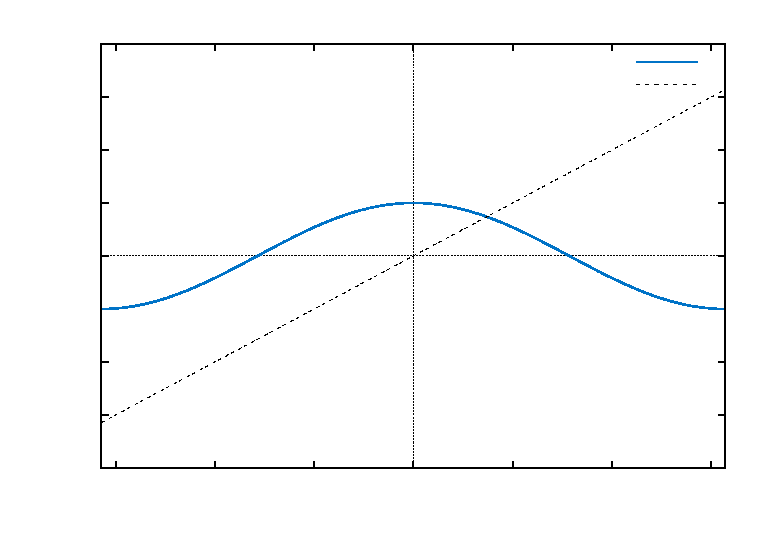
\includegraphics{cosineeqx}}%
    \gplfronttext
  \end{picture}%
\endgroup
\vspace{-6mm}
 \end{center}
 \caption[]{\quad $y=\cos\;x$ and $y=x$}
 \label{fig:cosineeqx}
\end{figure}

Unfortunately
there is no trigonometric identity or simple method which will help us here. Instead, we have to
resort to \emph{numerical methods}\index{numerical methods}, which provide ways of getting
successively better approximations to the actual solution(s) to within any desired degree of
accuracy. There is a large field of mathematics devoted to this subject called \emph{numerical
analysis}. Many of the methods require calculus, but luckily there is a method which we can use
that requires just basic algebra. It is called the \emph{secant method}\index{secant method}, and it
finds roots of a given function $f(x)$, i.e. values of $x$ such that $f(x)=0$. A derivation of the
secant method is beyond the scope of this book,\footnote{For an explanation of why the secant method
 works, see pp. 338-344 in \textsc{A. Ralston and P. Rabinowitz}, \emph{A First Course in Numerical
 Analysis}, 2nd ed., New York: McGraw-Hill Book Co., 1978.} but we can state the algorithm it
 uses to solve $f(x)=0$:

\begin{enumerate}[\bfseries 1.]
 \item Pick initial points $x_0$ and $x_1$ such that $x_0 < x_1$ and $f(x_0)\,f(x_1) < 0$ (i.e.
  the solution is somewhere between $x_0$ and $x_1$).
 \item For $n \ge 2$, define the number $x_n$ by
  \begin{equation}\label{eqn:secantmethod}
   x_n ~=~ x_{n-1} ~-~ \dfrac{(x_{n-1} \;-\; x_{n-2})\,f(x_{n-1})}{f(x_{n-1}) \;-\; f(x_{n-2})}
  \end{equation}
  as long as $\abs{x_{n-1} \;-\; x_{n-2}} > \epsilon_{error}$, where $\epsilon_{error} > 0$ is the
  maximum amount of error desired (usually a very small number).
 \item The numbers $x_0$, $x_1$, $x_2$, $x_3$, $...$ will approach the solution $x$ as we go through
 more iterations, getting as close as desired.
\end{enumerate}

We will now show how to use this algorithm to solve the equation $\cos\;x = x$. The solution to that
equation is the root of the function $f(x) =\cos\;x - x$. And we saw that the solution is somewhere
in the interval $\ival{0}{1}$. So pick $x_0 = 0$ and $x_1 = 1$. Then $f(0)=1$ and $f(1)=-0.4597$, so
that $f(x_0)\,f(x_1) < 0$ (we are using radians, of course). Then by definition,
\begin{align*}
 x_2 ~&=~ x_1 ~-~ \dfrac{(x_1 \;-\; x_0)\,f(x_1)}{f(x_1) \;-\; f(x_0)}\\
 &=~ 1 ~-~ \dfrac{(1 \;-\; 0)\,f(1)}{f(1) \;-\; f(0)}\\
 &=~ 1 ~-~ \dfrac{(1 \;-\; 0)\,(-0.4597)}{-0.4597 \;-\; 1}\\
 &=~ 0.6851~,\\
 x_3 ~&=~ x_2 ~-~ \dfrac{(x_2 \;-\; x_1)\,f(x_2)}{f(x_2) \;-\; f(x_1)}\\
 &=~ 0.6851 ~-~ \dfrac{(0.6851 \;-\; 1)\,f(0.6851)}{f(0.6851) \;-\; f(1)}\\
 &=~ 0.6851 ~-~ \dfrac{(0.6851 \;-\; 1)\,(0.0893)}{0.0893 \;-\; (-0.4597)}\\
 &=~ 0.7363 ~,
\end{align*}
and so on. Using a calculator is not very efficient and will lead to rounding errors. A better way
to implement the algorithm is with a computer. Listing \ref{lst:secant} below shows the code
(secant.java) for solving $\cos\;x = x$ with the secant method, using the Java programming language:

\lstset{language=Java,showstringspaces=false,lineskip=1pt,
basicstyle={\small\fontfamily{fvm}\fontseries{m}\selectfont},
columns=fullflexible,backgroundcolor=\color{codecolor},numbers=left,
numberstyle={\color{linenumcolor}\footnotesize\fontfamily{fvm}\fontseries{m}\selectfont},
commentstyle={\color{black}\small\fontfamily{fvm}\itshape\selectfont},
keywordstyle={\small\fontfamily{fvm}\fontseries{m}\selectfont},keepspaces=true,
float=h,caption={\quad Program listing for secant.java},numbersep=15pt,label=lst:secant}
\begin{center}\begin{minipage}[t]{13cm}
\begin{lstlisting}[frame=single,framerule=0pt]
import java.math.*;
public class secant {
 public static void main (String[] args) {
   double x0 =  Double.parseDouble(args[0]);
   double x1 =  Double.parseDouble(args[1]);
   double x = 0;
   double error = 1.0E-50;
   for (int i=2; i <= 10; i++) {
      if (Double.compare(Math.abs(x0 - x1),error) > 0) {
         x = x1 - (x1 - x0)*f(x1)/(f(x1) - f(x0));
         x0 = x1;
         x1 = x;
         System.out.println("x" + i + " = " + x);
      } else {
         break;
      }
   }
   MathContext mc = new MathContext(50);
   BigDecimal answer = new BigDecimal(x,mc);
   System.out.println("x = " + answer);
 }
//Define the function f(x)
 public static double f (double x) {
   return Math.cos(x) - x;
 }
}
\end{lstlisting}
\end{minipage}\end{center}

\par\noindent Lines 4-5 read in $x_0$ and $x_1$ as input parameters to the program.

\par\noindent Line 6 initializes the variable that will eventually hold the solution.

\par\noindent Line 7 sets the maximum error $\epsilon_{error}$ to be $1.0 \,\times\, 10^{-50}$. That
is, our final answer will be within that (tiny!) amount of the real solution.

\par\noindent Line 8 starts a loop of 9 iterations of the algorithm, i.e. it will create the
successive approximations $x_2$, $x_3$, $...$, $x_{10}$ to the real solution, though in Line 9 we
check to see if the two previous approximations differ by less than the maximum error. If they do,
we stop (since this means we have an acceptable solution), otherwise we continue.

\par\noindent Line 10 is the main step in the algorithm, creating $x_n$ from $x_{n-1}$ and
$x_{n-2}$.

\par\noindent Lines 11-12 set the new values of $x_{n-2}$ and $x_{n-1}$, respectively.

\par\noindent Lines 18-20 set the number of decimal places to show in the final answer
to 50 (the default is 16) and then print the answer.

\par\noindent Lines 23-24 give the definition of the function $f(x)=\cos\;x - x$.
\newpage
Below is the result of compiling and running the program using $x_0 = 0$ and $x_1 = 1$:

\begin{verbatim}
javac secant.java
java secant 0 1
x2 = 0.6850733573260451
x3 = 0.736298997613654
x4 = 0.7391193619116293
x5 = 0.7390851121274639
x6 = 0.7390851332150012
x7 = 0.7390851332151607
x8 = 0.7390851332151607
x = 0.73908513321516067229310920083662495017051696777344
\end{verbatim}

Notice that the program only got up to $x_8$, not $x_{10}$. The reason is that the difference
between $x_8$ and $x_7$ was small enough (less than $\epsilon_{error} = 1.0 \,\times\, 10^{-50}$)
to stop at $x_8$ and call that our solution.
The last line shows that solution to 50 decimal places.

Does that number look familiar? It should, since it is the answer to Exercise \ref{exer:cosxeqx} in
Section 4.1. That is, when taking repeated cosines starting with any number (in radians), you
eventually start getting the above number repeatedly after enough iterations. This turns out not to
be a coincidence. Figure \ref{fig:cosinefixed} gives an idea of why.

\begin{figure}[h]
 \begin{center}
  % GNUPLOT: LaTeX picture with Postscript
\begingroup
\footnotesize
  \makeatletter
  \providecommand\color[2][]{%
    \GenericError{(gnuplot) \space\space\space\@spaces}{%
      Package color not loaded in conjunction with
      terminal option `colourtext'%
    }{See the gnuplot documentation for explanation.%
    }{Either use 'blacktext' in gnuplot or load the package
      color.sty in LaTeX.}%
    \renewcommand\color[2][]{}%
  }%
  \providecommand\includegraphics[2][]{%
    \GenericError{(gnuplot) \space\space\space\@spaces}{%
      Package graphicx or graphics not loaded%
    }{See the gnuplot documentation for explanation.%
    }{The gnuplot epslatex terminal needs graphicx.sty or graphics.sty.}%
    \renewcommand\includegraphics[2][]{}%
  }%
  \providecommand\rotatebox[2]{#2}%
  \@ifundefined{ifGPcolor}{%
    \newif\ifGPcolor
    \GPcolortrue
  }{}%
  \@ifundefined{ifGPblacktext}{%
    \newif\ifGPblacktext
    \GPblacktexttrue
  }{}%
  % define a \g@addto@macro without @ in the name:
  \let\gplgaddtomacro\g@addto@macro
  % define empty templates for all commands taking text:
  \gdef\gplbacktext{}%
  \gdef\gplfronttext{}%
  \makeatother
  \ifGPblacktext
    % no textcolor at all
    \def\colorrgb#1{}%
    \def\colorgray#1{}%
  \else
    % gray or color?
    \ifGPcolor
      \def\colorrgb#1{\color[rgb]{#1}}%
      \def\colorgray#1{\color[gray]{#1}}%
      \expandafter\def\csname LTw\endcsname{\color{white}}%
      \expandafter\def\csname LTb\endcsname{\color{black}}%
      \expandafter\def\csname LTa\endcsname{\color{black}}%
      \expandafter\def\csname LT0\endcsname{\color[rgb]{1,0,0}}%
      \expandafter\def\csname LT1\endcsname{\color[rgb]{0,1,0}}%
      \expandafter\def\csname LT2\endcsname{\color[rgb]{0,0,1}}%
      \expandafter\def\csname LT3\endcsname{\color[rgb]{1,0,1}}%
      \expandafter\def\csname LT4\endcsname{\color[rgb]{0,1,1}}%
      \expandafter\def\csname LT5\endcsname{\color[rgb]{1,1,0}}%
      \expandafter\def\csname LT6\endcsname{\color[rgb]{0,0,0}}%
      \expandafter\def\csname LT7\endcsname{\color[rgb]{1,0.3,0}}%
      \expandafter\def\csname LT8\endcsname{\color[rgb]{0.5,0.5,0.5}}%
    \else
      % gray
      \def\colorrgb#1{\color{black}}%
      \def\colorgray#1{\color[gray]{#1}}%
      \expandafter\def\csname LTw\endcsname{\color{white}}%
      \expandafter\def\csname LTb\endcsname{\color{black}}%
      \expandafter\def\csname LTa\endcsname{\color{black}}%
      \expandafter\def\csname LT0\endcsname{\color{black}}%
      \expandafter\def\csname LT1\endcsname{\color{black}}%
      \expandafter\def\csname LT2\endcsname{\color{black}}%
      \expandafter\def\csname LT3\endcsname{\color{black}}%
      \expandafter\def\csname LT4\endcsname{\color{black}}%
      \expandafter\def\csname LT5\endcsname{\color{black}}%
      \expandafter\def\csname LT6\endcsname{\color{black}}%
      \expandafter\def\csname LT7\endcsname{\color{black}}%
      \expandafter\def\csname LT8\endcsname{\color{black}}%
    \fi
  \fi
  \setlength{\unitlength}{0.0500bp}%
  \begin{picture}(7200.00,5040.00)%
    \gplgaddtomacro\gplbacktext{%
      \csname LTb\endcsname%
      \put(946,704){\makebox(0,0)[r]{\strut{} 0}}%
      \put(946,1518){\makebox(0,0)[r]{\strut{} 0.2}}%
      \put(946,2332){\makebox(0,0)[r]{\strut{} 0.4}}%
      \put(946,3147){\makebox(0,0)[r]{\strut{} 0.6}}%
      \put(946,3961){\makebox(0,0)[r]{\strut{} 0.8}}%
      \put(946,4775){\makebox(0,0)[r]{\strut{} 1}}%
      \put(1078,484){\makebox(0,0){\strut{}$-\frac{\pi}{2}$}}%
      \put(2118,484){\makebox(0,0){\strut{}-1}}%
      \put(3941,484){\makebox(0,0){\strut{}0}}%
      \put(5763,484){\makebox(0,0){\strut{}1}}%
      \put(6803,484){\makebox(0,0){\strut{}$\frac{\pi}{2}$}}%
      \csname LTb\endcsname%
      \put(176,2739){\rotatebox{-270}{\makebox(0,0){\strut{}$y$}}}%
      \put(3940,154){\makebox(0,0){\strut{}$x$}}%
    }%
    \gplgaddtomacro\gplfronttext{%
      \csname LTb\endcsname%
      \put(1754,3961){\makebox(0,0)[l]{\strut{}$y = \cos(x)$}}%
      \put(4669,1925){\makebox(0,0)[l]{\strut{}$y = x$}}%
    }%
%    \gplgaddtomacro\gplbacktext{%
%      \put(946,704){\makebox(0,0)[r]{\strut{} 0}}%
%      \put(946,1518){\makebox(0,0)[r]{\strut{} 0.2}}%
%      \put(946,2332){\makebox(0,0)[r]{\strut{} 0.4}}%
%      \put(946,3147){\makebox(0,0)[r]{\strut{} 0.6}}%
%      \put(946,3961){\makebox(0,0)[r]{\strut{} 0.8}}%
%      \put(946,4775){\makebox(0,0)[r]{\strut{} 1}}%
%      \put(1078,484){\makebox(0,0){\strut{}$-\frac{\pi}{2}$}}%
%      \put(2118,484){\makebox(0,0){\strut{}-1}}%
%      \put(3941,484){\makebox(0,0){\strut{}0}}%
%      \put(5763,484){\makebox(0,0){\strut{}1}}%
%      \put(6803,484){\makebox(0,0){\strut{}$\frac{\pi}{2}$}}%
%      \csname LTb\endcsname%
%      \put(176,2739){\rotatebox{-270}{\makebox(0,0){\strut{}$y$}}}%
%      \put(3940,154){\makebox(0,0){\strut{}$x$}}%
%    }%
%    \gplgaddtomacro\gplfronttext{%
%      \csname LTb\endcsname%
%      \put(1754,3961){\makebox(0,0)[l]{\strut{}$y = \cos(x)$}}%
%      \put(4669,1925){\makebox(0,0)[l]{\strut{}$y = x$}}%
%    }%
%    \gplgaddtomacro\gplbacktext{%
%      \put(946,704){\makebox(0,0)[r]{\strut{} 0}}%
%      \put(946,1518){\makebox(0,0)[r]{\strut{} 0.2}}%
%      \put(946,2332){\makebox(0,0)[r]{\strut{} 0.4}}%
%      \put(946,3147){\makebox(0,0)[r]{\strut{} 0.6}}%
%      \put(946,3961){\makebox(0,0)[r]{\strut{} 0.8}}%
%      \put(946,4775){\makebox(0,0)[r]{\strut{} 1}}%
%      \put(1078,484){\makebox(0,0){\strut{}$-\frac{\pi}{2}$}}%
%      \put(2118,484){\makebox(0,0){\strut{}-1}}%
%      \put(3941,484){\makebox(0,0){\strut{}0}}%
%      \put(5763,484){\makebox(0,0){\strut{}1}}%
%      \put(6803,484){\makebox(0,0){\strut{}$\frac{\pi}{2}$}}%
%      \csname LTb\endcsname%
%      \put(176,2739){\rotatebox{-270}{\makebox(0,0){\strut{}$y$}}}%
%      \put(3940,154){\makebox(0,0){\strut{}$x$}}%
%    }%
%    \gplgaddtomacro\gplfronttext{%
%      \csname LTb\endcsname%
%      \put(1754,3961){\makebox(0,0)[l]{\strut{}$y = \cos(x)$}}%
%      \put(4669,1925){\makebox(0,0)[l]{\strut{}$y = x$}}%
%    }%
    \gplbacktext
    \put(0,0){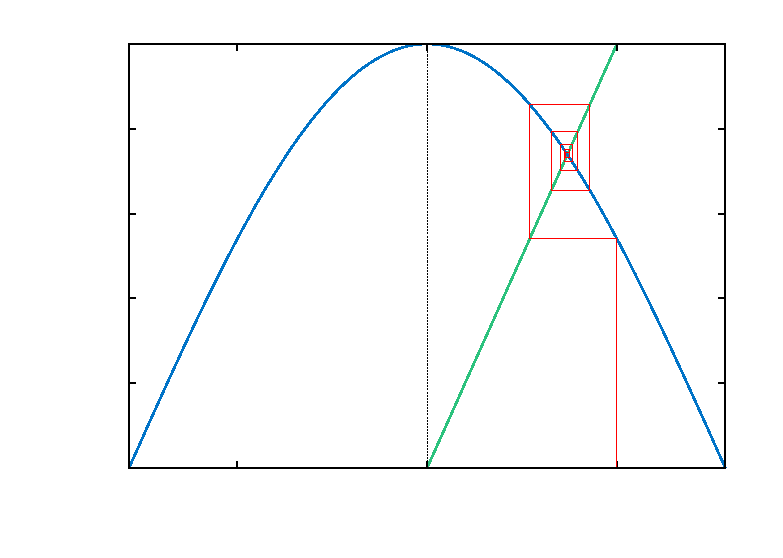
\includegraphics{cosinefixed}}%
    \gplfronttext
  \end{picture}%
\endgroup
\vspace{-6mm}
 \end{center}
 \caption[]{\quad Attractive fixed point for $\cos\;x$}
 \label{fig:cosinefixed}
\end{figure}
%\newpage
Since $x=0.73908513321516...$ is the solution of $\cos\;x = x$, you would get
$\cos\;(\cos\;x) = \cos\;x = x$, so $\cos\;(\cos\;(\cos\;x)) = \cos\;x = x$, and so on. This number
$x$ is called an \emph{attractive fixed point} of the function $\cos\;x$. No matter where you
start, you end up getting ``drawn'' to it. Figure \ref{fig:cosinefixed} shows what happens when
starting at $x=0$: taking the cosine of $0$ takes you to $1$, and then successive cosines (indicated
by the intersections of the vertical lines with the cosine curve) eventually ``spiral'' in a
rectangular fashion to the fixed point (i.e. the solution), which is the intersection of $y=\cos\;x$
and $y=x$.\index{attractive fixed point}

Recall in Example \ref{exmp:cos6xsin4x} in Section 5.2 that we claimed that the maximum and minimum
of the function $y=\cos\;6x + \sin\;4x$ were $\pm\,1.90596111871578$, respectively. We can show this
by using the open-source program Octave.\footnote{Freely available at
\url{http://www.gnu.org/software/octave}} Octave uses a \emph{successive quadratic
 programming} method to find the minimum of a function $f(x)$. Finding the maximum of $f(x)$ is the
same as finding the minimum of $-f(x)$ then multiplying by $-1$ (why?). Below we show the commands
to run at the Octave command prompt (\texttt{octave:n>}) to find the minimum of $f(x) =
\cos\;6x + \sin\;4x$. The command \texttt{sqp(3,'f')} says to use $x=3$ as a first approximation
of the number $x$ where $f(x)$ is a minimum.
 
\begin{Verbatim}[frame=single,framesep=2mm]
octave:1> format long
octave:2> function y = f(x)
> y = cos(6*x) + sin(4*x)
> endfunction
octave:3> sqp(3,'f')
y = -1.90596111871578
ans = 2.65792064609274
\end{Verbatim}

The output says that the minimum occurs when $x=2.65792064609274$ and that the minimum is
$-1.90596111871578$. To find the maximum of $f(x)$, we find the minimum of $-f(x)$ and then take
its negative. The command \texttt{sqp(2,'f')} says to use $x=2$ as a first approximation
of the number $x$ where $f(x)$ is a maximum.

\begin{Verbatim}[frame=single,framesep=1mm]
octave:4> function y = f(x)
> y = -cos(6*x) - sin(4*x)
> endfunction
octave:5> sqp(2,'f')
y = -1.90596111871578
ans = 2.05446832062993
\end{Verbatim}

The output says that the maximum occurs when $x=2.05446832062993$
and that the maximum is $-(-1.90596111871578) = 1.90596111871578$.

Recall from Section 2.4 that Heron's formula is adequate for ``typical'' triangles, but will often
have a problem
when used in a calculator with, say, a triangle with two sides whose sum is barely larger than the
third side. However, you can get around this problem by using computer software capable of handling
numbers with a high degree of precision. Most modern computer programming languages have this
capability. For example, in the Python programming language\footnote{Available for free at
\url{http://www.python.org}} (chosen here for simplicity) the \texttt{decimal} module can be used
to set any level of precision.\footnote{Other languages have similar capability, e.g. the
\texttt{BigDecimal} class in Java.} Below we show how to get accuracy up to $50$ decimal places
using Heron's formula for the triangle in Example \ref{exmp:heronfail} from Section 2.4, by using
the python interactive command shell:

\begin{Verbatim}[frame=single,framesep=1mm]
>>> from decimal import *
>>> getcontext().prec = 50
>>> a = Decimal("1000000")
>>> b = Decimal("999999.9999979")
>>> c = Decimal("0.0000029")
>>> s = (a+b+c)/2
>>> K = s*(s-a)*(s-b)*(s-c)
>>> print Decimal(K).sqrt()
0.99999999999894999999999894874999999889618749999829
\end{Verbatim}

\noindent(Note: The triple arrow \texttt{\symbol{62}\symbol{62}\symbol{62}} is
just a command prompt, not part of the code.)\\Notice in this case that we do
get the correct answer; the high level of precision eliminates the
rounding errors shown by many calculators when using Heron's formula.

Another software option is
Sage\footnote{Visit the homepage at \url{http://www.sagemath.org} for more details.}, a
powerful and free open-source mathematics package based on Python. It can be run on your
own computer, but it can also be run through a web interface: go to \url{http://sagenb.org} to
create a free account, then once you register and sign in, click the
\textbf{New Worksheet} link to start entering commands. For example, to find the solution to
$\cos\;x = x$ in the interval $\ival{0}{1}$, enter these commands in the worksheet textfield:

\begin{Verbatim}[frame=single,framesep=1mm]
x = var('x')
find_root(cos(x) == x, 0,1)
\end{Verbatim}

\noindent Click the \textbf{evaluate} link to display the answer: $0.7390851332151559$\vspace{1mm}

\divider
\vspace{2mm}

\startexercises\label{sec6dot2}
\vspace{4mm}
{\small
\begin{enumerate}[\bfseries 1.]
 \item One obvious solution to the equation $2\,\sin\;x = x$ is $x=0$.
 Write a program to find the other solution(s), accurate to at least
 within $1.0 \,\times\, 10^{-20}$. You can use any programming language, though you may find it
 easier to just modify the code in Listing \ref{lst:secant} (only one line needs to be changed!).
 It may help to use Gnuplot to get an idea of where the graphs of $y=2\,\sin\;x$ and $y=x$
 intersect.
 \item Repeat Exercise 1 for the equation $\sin\;x = x^2$.
 \item Use Octave or some other program to find the maximum and minimum of $y=\cos\;5x - \sin\;3x$.
\end{enumerate}}
\newpage
%Begin Section 6.3
\section{Complex Numbers}
There is no real number $x$ such that $x^2 = -1$. However, it turns out to be
useful\footnote{Especially in electrical engineering, physics, and various fields of mathematics.}
to invent such a
number, called the \textbf{imaginary unit}\index{imaginary unit} and denoted by the letter $i$.
Thus, $i^2 = -1$, and hence $i = \sqrt{-1}$. If $a$ and $b$ are real numbers, then a number of the
form $a + bi$ is called a \textbf{complex number}\index{complex number}, and if $b \ne 0$ then it
is called an \textbf{imaginary number}\index{imaginary number} (and \textbf{pure
imaginary}\index{pure imaginary number}\index{imaginary number!pure} if $a=0$ and $b \ne 0$).
The real number $a$ is called the \textbf{real part}\index{real part} of the complex
number $a+bi$, and $bi$ is called its \textbf{imaginary part}\index{imaginary part}.

What does it mean to add $a$ to $bi$ in the definition $a+bi$ of a complex number, i.e. adding a
real number and an imaginary number? You can think of it as a way of \emph{extending} the set of
real numbers. If $b=0$ then $a+bi = a+0i = a$ (since $0i$ is defined as $0$), so that every real
number is a complex number.
The imaginary part $bi$ in $a+bi$ can be thought of as a way of taking the \emph{one-dimensional}
set of all real numbers and extending it to a \emph{two-dimensional} set: there is a natural
correspondence between a complex number $a+bi$ and a \emph{point} $(a,b)$ in the
(two-dimensional) $xy$-coordinate plane.

Before exploring that correspondence further, we will first state some fundamental properties of
and operations on complex numbers:

\begin{center}\statecomment{Let $a+bi$ and $c+di$ be complex numbers. Then:
\begin{enumerate}[\bfseries 1.]
 \item $a+bi ~=~ c+di$ if and only if $a=c$ and $b=d~$ (i.e. the real parts are equal and the
 imaginary parts are equal)
 \item $(a+bi) \;+\; (c+di) ~=~ (a+c) \;+\; (b+d)i~$ (i.e. add the real parts together and add the
 imaginary parts together)
 \item $(a+bi) \;-\; (c+di) ~=~ (a-c) \;+\; (b-d)i$
 \item $(a+bi)\,(c+di) ~=~ (ac-bd) \;+\; (ad+bc)i$
 \item $(a+bi)\,(a-bi) ~=~ a^2 \;+\; b^2$
 \item $\dfrac{a+bi}{c+di} ~=~ \dfrac{(ac+bd) \;+\; (bc-ad)i}{c^2 + d^2}$
\end{enumerate}}\end{center}

The first three items above are just definitions of equality, addition, and subtraction of complex
numbers. The last three items can be derived by treating the multiplication and division of complex
numbers as you would normally treat factors of real numbers:
\begin{align*}
 (a+bi)\,(c+di) ~&=~ a\,(c+di) \;+\; bi\,(c+di)\\
 &=~ ac \;+\; adi \;+\; bci \;+\; bdi^2 ~=~ ac \;+\; adi \;+\; bci \;+\; bd(-1)\\
 &=~ (ac - bd) \;+\; (ad+bc)i
\end{align*}
\newpage
\noindent The fifth item is a special case of the multiplication formula:
\begin{align*}
 (a+bi)\,(a-bi) ~&=~ ((a)(a) - (b)(-b)) \;+\; ((a)(-b) + (b)(a))i\\
 &=~ ( a^2 + b^2 ) \;+\; (-ab + ba)i ~=~ ( a^2 + b^2 ) \;+\; 0i\\
 &=~ a^2 \;+\; b^2
\end{align*}
The sixth item comes from using the previous items:
\begin{align*}
 \dfrac{a+bi}{c+di} ~&=~ \dfrac{a+bi}{c+di} \,\cdot\, \dfrac{c-di}{c-di}\\
 &=~ \dfrac{(ac - b(-d)) \;+\; (a(-d) + bc)i}{c^2 + d^2}\\
 &=~ \dfrac{(ac+bd) \;+\; (bc-ad)i}{c^2 + d^2}
\end{align*}

The \textbf{conjugate}\index{conjugate} $\overline{a+bi}$ of a complex number $a+bi$ is defined as
$\overline{a+bi} = a-bi$. Notice that $(a+bi) \;+\; \overline{(a+bi)} ~=~ 2a$ is a real number,
$(a+bi) \;-\; \overline{(a+bi)} ~=~ 2bi$ is an imaginary number if $b \ne 0$, and
$(a+bi) \overline{(a+bi)} ~=~ a^2 + b^2$ is a real number. So for a complex number $z=a+bi$,
$z\,\overline{z} = a^2 + b^2 \,$ and thus we can define the \textbf{modulus}\index{modulus} of $z$
to be $\sqrt{z\,\overline{z}} = \sqrt{a^2 + b^2}$, which we denote by $\abs{z}$.\index{complex
number!modulus of}\index{complex number!conjugate of}

\begin{exmp}
 Let $z_1 = -2+3i$ and $z_2 = 3+4i$. Find $z_1 + z_2$, $z_1 - z_2$, $z_1 \, z_2$, $z_1 / z_2$,
 $\abs{z_1}$, and $\abs{z_2}$.\vspace{1mm}
 \par\noindent\textbf{Solution:} Using our rules and definitions, we have:
 \begin{align*}
  z_1 \;+\; z_2 ~&=~ (-2+3i) \;+\; (3+4i)\\
  &=~ 1 + 7i\\
  z_1 \;-\; z_2 ~&=~ (-2+3i) \;-\; (3+4i)\\
  &=~ -5 - i\\
  z_1 \, z_2 ~&=~ (-2+3i)\, (3+4i)\\
  &=~ ((-2)(3) - (3)(4)) \;+\; ((-2)(4) + (3)(3))i\\
  &=~ -18 + i\\
  \dfrac{z_1}{z_2} ~&=~ \dfrac{-2+3i}{3+4i}\\
  &=~ \dfrac{(-2)(3) + (3)(4) \;+\; ((3)(3) - (-2)(4))i}{3^2 + 4^2}\\
  &=~ \dfrac{6}{25} \;+\; \dfrac{17}{25}\,i\\
  \abs{z_1} ~&=~ \sqrt{(-2)^2 + 3^2}\\
  &=~ \sqrt{13}\\
  \abs{z_2} ~&=~ \sqrt{3^2 + 4^2}\\
  &=~ 5
 \end{align*}
\end{exmp}
\divider
\newpage
We know that any point $(x,y)$ in the $xy$-coordinate plane that is a distance $r >0$ from the
origin has coordinates $x=r\,\cos\;\theta$ and $y=r\,\sin\;\theta$, where $\theta$ is the angle in
standard position as in Figure \ref{fig:complex}(a).

\begin{figure}[h]
 \centering
 \subfloat[][ Point $(x,y)$]{
 \begin{tikzpicture}[every node/.style={font=\small}]
  \draw [line width=0.5pt,-latex] (0.8,0) arc (0:55:0.8);
  \draw [black!60,line width=0.3pt,-latex] (-0.5,0) -- (3,0) node [right] {$x$};
  \draw [black!60,line width=0.3pt,-latex] (0,-0.5) -- (0,2.6) node [above] {$y$};
  \node [black!60,below left] at (0,0) {$0$};
  \node [right] at (30:0.4) {$\theta$};
  \draw [dashed] (0,0) -- (55:2.5) node[above left,midway] {$r$};
  \fill (55:2.5) circle (2pt) node[above right] {$(x,y)=(r\,\cos\;\theta , r\,\sin\;\theta)$};
\end{tikzpicture}}
 \qquad\qquad
 \subfloat[][ Complex number $z=x+yi$]{
 \begin{tikzpicture}[every node/.style={font=\small}]
  \draw [line width=0.5pt,-latex] (0.8,0) arc (0:55:0.8);
  \draw [black!60,line width=0.3pt,-latex] (-0.5,0) -- (3,0) node [right] {$x$};
  \draw [black!60,line width=0.3pt,-latex] (0,-0.5) -- (0,2.6) node [above] {$y$};
  \node [black!60,below left] at (0,0) {$0$};
  \node [right] at (30:0.4) {$\theta$};
  \draw [dashed] (0,0) -- (55:2.5) node[above left,midway] {$r$};
  \fill (55:2.5) circle (2pt) node[above right] {$z=x+yi = r\,\cos\;\theta\,+\,(r\,\sin\;\theta)i$};
 \end{tikzpicture}}
 \caption[]{}
 \label{fig:complex}
\end{figure}

Let $z=x+yi$ be a complex number. We can represent $z$ as a point in the \textbf{complex
plane},\index{complex plane} where the horizontal $x$-axis represents the real part of $z$, and the
vertical $y$-axis represents the pure imaginary\index{complex plane}
part of $z$, as in Figure \ref{fig:complex}(b). The distance $r$ from $z$ to the origin is, by the
Pythagorean Theorem, $r = \sqrt{x^2 + y^2}$, which is just the modulus of $z$. And we see from
Figure \ref{fig:complex}(b) that $x=r\,\cos\;\theta$ and $y=r\,\sin\;\theta$, where $\theta$ is the
angle formed by the positive $x$-axis and the line segment from the origin to $z$. We call this
angle $\theta$ the \textbf{argument}\index{argument of a complex number}\index{complex
number!argument of} of $z$. Thus, we get the
\textbf{trigonometric form}\index{trigonometric form}\index{complex number!trigonometric form}
(sometimes called the \emph{polar form}) of the complex number $z$:

\begin{center}\statecomment{For any complex number $z=x+yi$, we can write
\begin{align}
 z ~&=~ r\,(\cos\;\theta \;+\; i\,\sin\;\theta)~~,~\text{where}\label{eqn:polar}\\
 r ~&=~ \abs{z} ~=~ \sqrt{x^2 + y^2}~~\text{and}\notag\\
 \theta ~&=~ \text{the argument of $z$}~.\notag\\
 \intertext{The representation $z=r\,(\cos\;\theta \;+\; i\,\sin\;\theta)$ is often abbreviated as:}
 z ~&=~ r\,\text{cis}\;\theta\label{eqn:cis}
\end{align}}\end{center}

In the special case $z=0 = 0+0i$, the argument $\theta$ is undefined since $r=\abs{z}=0$. Also, note
that the argument $\theta$ can be replaced by $\theta \;+\; 360\Degrees k$ or $\theta \;+\; \pi k$,
depending on whether you are using degrees or radians, respectively, for $k=0$, $\pm\,1$, $\pm\,2$,
$...$ .\index{cis} Note also that for $z=x+yi$ with $r=\abs{z}$, $\theta$ must satisfy
\begin{displaymath}
 \tan\;\theta ~=~ \tfrac{y}{x}~~,~ \cos\;\theta ~=~ \tfrac{x}{r}~~,~ \sin\;\theta ~=~ \tfrac{y}{r}~.
\end{displaymath}
\newpage
\begin{exmp}
\piccaption[]{\label{fig:exmppolar}}\parpic[r]{\begin{tikzpicture}[every node/.style={font=\small}]
 \draw[black!60,solid,line width=0.3pt,-latex] (-2.1,0) -- (0.7,0) node[right] {$x$};
 \draw[black!60,solid,line width=0.3pt,-latex] (0,-1.1) -- (0,0.7) node[above] {$y$};
 \node[black,below right] at (0,0) {$0$};
 \fill (-2,-1) circle (2pt);
 \draw [dashed] (-2,-1) -- (0,0) node [midway,below] {$r$};
 \draw [dashed] (-2,-1) -- (-2,0) node [midway,left] {$1$};
 \node [above] at (-1.2,0) {$2$};
 \node [below] at (-1.4,-1) {$z=-2-i$};
 \draw [-latex] (0:0.45) arc (0:206.56:0.45);
 \node [left] at (120:0.5) {$\theta$};
\end{tikzpicture}}
\noindent Represent the complex number $-2 - i$ in trigonometric form.\vspace{1mm}
 \par\noindent\textbf{Solution:} Let $z=-2-i=x+yi$, so that $x=-2$ and $y=-1$. Then $\theta$ is in
  QIII, as we see in Figure \ref{fig:exmppolar}. So since $\tan\;\theta = \tfrac{y}{x} =
  \tfrac{-1}{-2} = \tfrac{1}{2}$, we have $\theta = 206.6\Degrees$. Also,
 \begin{displaymath}
  r ~=~ \sqrt{x^2 + y^2} ~=~ \sqrt{(-2)^2 + (-1)^2} ~=~ \sqrt{5} ~.
 \end{displaymath}
 Thus, $\boxed{-2 - i = \sqrt{5}\;(\cos\;206.6\Degrees \;+\; i\,\sin\;206.6\Degrees)}\;$, or
 $\sqrt{5}\;\text{cis}\;206.6\Degrees$.
\end{exmp}
\divider
\vspace{1mm}

For complex numbers in trigonometric form, we have the following formulas for multiplication and
division:

\begin{center}\statecomment{Let $z_1 = r_1 \,(\cos\;\theta_1 \;+\; i\,\sin\;\theta_1 )$ and
$z_2 = r_2 \,(\cos\;\theta_2 \;+\; i\,\sin\;\theta_2 )$ be complex numbers. Then
\begin{align}
 z_1 \, z_2 ~&=~ r_1 \, r_2 \,(\cos\;(\theta_1 + \theta_2 ) \;+\; i\,\sin\;(\theta_1 +
  \theta_2 ))~\text{, and}\label{eqn:complextrigmult}\\
 \frac{z_1}{z_2} ~&=~ \frac{r_1}{r_2} \,(\cos\;(\theta_1 - \theta_2 ) \;+\; i\,\sin\;(\theta_1 -
  \theta_2 ))\quad\text{if $z_2 \ne 0$.}\label{eqn:complextrigdiv}
\end{align}}\end{center}

\noindent The proofs of these formulas are straightforward:
\begin{align*}
 z_1 \, z_2 ~&=~ r_1 \,(\cos\;\theta_1 \;+\; i\,\sin\;\theta_1 ) \;\cdot\;
  r_2 \,(\cos\;\theta_2 \;+\; i\,\sin\;\theta_2 )\\
 &=~ r_1 \, r_2 \,\left[ (\cos\;\theta_1 ~ \cos\;\theta_2 \;-\; \sin\;\theta_1 ~ \sin\;\theta_2 )
  \;+\; i\,(\sin\;\theta_1 ~ \cos\;\theta_2 \;+\; \cos\;\theta_1 ~ \sin\;\theta_2 ) \right]\\
 &=~ r_1 \, r_2 \,(\cos\;(\theta_1 + \theta_2 ) \;+\; i\,\sin\;(\theta_1 + \theta_2 ))\\
 \intertext{by the addition formulas for sine and cosine. And}
 \frac{z_1}{z_2} ~&=~ \frac{r_1 \,(\cos\;\theta_1 \;+\; i\,\sin\;\theta_1 )}{
  r_2 \,(\cos\;\theta_2 \;+\; i\,\sin\;\theta_2 )}\\
 &=~ \frac{r_1}{r_2} \;\cdot\; \frac{\cos\;\theta_1 \;+\; i\,\sin\;\theta_1}{
  \cos\;\theta_2 \;+\; i\,\sin\;\theta_2} \;\cdot\; \frac{\cos\;\theta_2 \;-\; i\,\sin\;\theta_2}{
  \cos\;\theta_2 \;-\; i\,\sin\;\theta_2}\\
 &=~ \frac{r_1}{r_2} \;\cdot\; \frac{(\cos\;\theta_1 ~ \cos\;\theta_2 \;+\; \sin\;\theta_1 ~
  \sin\;\theta_2 ) \;+\; i\,(\sin\;\theta_1 ~ \cos\;\theta_2 \;-\; \cos\;\theta_1 ~
  \sin\;\theta_2 )}{\cos^2 \,\theta_2 \;+\; \sin^2 \,\theta_2}\\
 &=~ \frac{r_1}{r_2} \,(\cos\;(\theta_1 - \theta_2 ) \;+\; i\,\sin\;(\theta_1 - \theta_2 ))
\end{align*}
by the subtraction formulas for sine and cosine, and since $\cos^2 \,\theta_2 \;+\;
\sin^2 \,\theta_2 = 1$. $\qed$

Note that formulas (\ref{eqn:complextrigmult}) and (\ref{eqn:complextrigdiv}) say that when
multiplying complex numbers the moduli are multiplied and the arguments are added, while when
dividing complex numbers the moduli are divided and the arguments are subtracted. This makes
working with complex numbers in trigonometric form fairly simple.
\newpage
\begin{exmp}
 Let $z_1 = 6\,(\cos\;70\Degrees \;+\; i\,\sin\;70\Degrees )$ and
 $z_1 = 2\,(\cos\;31\Degrees \;+\; i\,\sin\;31\Degrees )$. Find $z_1 \, z_2$ and
 $\frac{z_1}{z_2}$.\vspace{1mm}
 \par\noindent\textbf{Solution:} By formulas (\ref{eqn:complextrigmult}) and
 (\ref{eqn:complextrigdiv}) we have
\begin{alignat*}{3}
 z_1 \, z_2 ~&=~ (6) \, (2) \, (\cos\;(70\Degrees + 31\Degrees ) \;+\; i\,\sin\;(70\Degrees +
  31\Degrees )) \quad&&\Rightarrow\quad \boxed{z_1 \, z_2 ~=~ 12 \, (\cos\;101\Degrees \;+\;
  i\,\sin\;101\Degrees )} ~\text{, and}\\
 \frac{z_1}{z_2} ~&=~ \frac{6}{2} \, (\cos\;(70\Degrees - 31\Degrees ) \;+\; i\,\sin\;(70\Degrees -
  31\Degrees )) \quad&&\Rightarrow\quad \boxed{\frac{z_1}{z_2} ~=~ 3 \, (\cos\;39\Degrees \;+\;
  i\,\sin\;39\Degrees )} ~.
\end{alignat*}
\end{exmp}
\divider
\vspace{1mm}

For the special case when $z_1 = z_2 = z = r\,(\cos\;\theta \;+\; i\,\sin\;\theta)$ in formula
(\ref{eqn:complextrigmult}), we have
\begin{align*}
 \left[ r\,(\cos\;\theta \;+\; i\,\sin\;\theta)\right]^2 ~&=~
  r \cdot r \,(\cos\;(\theta + \theta ) \;+\; i\,\sin\;(\theta + \theta))\\
 &=~ r^2 \,(\cos\;2\theta \;+\; i\,\sin\;2\theta) ~,\\
 \intertext{and so}
 \left[ r\,(\cos\;\theta \;+\; i\,\sin\;\theta)\right]^3 ~&=~
  \left[ r\,(\cos\;\theta \;+\; i\,\sin\;\theta)\right]^2 \;\cdot\;
  r\,(\cos\;\theta \;+\; i\,\sin\;\theta )\\
 &=~ r^2 \,(\cos\;2\theta \;+\; i\,\sin\;2\theta) \;\cdot\;
  r\,(\cos\;\theta \;+\; i\,\sin\;\theta )\\
 &=~ r^3 \,(\cos\;(2\theta + \theta) \;+\; i\,\sin\;(2\theta + \theta) )\\
 &=~ r^3 \,(\cos\;3\theta \;+\; i\,\sin\;3\theta) ~,
\end{align*}
and continuing like this (i.e. by \emph{mathematical induction}), we get:\index{De Moivre's Theorem}

\statethm{thm:demoivre}{\textbf{De Moivre's Theorem:}\footnotemark \enskip For any integer $n \ge 1$,
\begin{equation}\label{eqn:demoivre}
 \left[ r\,(\cos\;\theta \;+\; i\,\sin\;\theta )\right]^n ~=~
 r^n \,(\cos\;n\theta \;+\; i\,\sin\;n\theta ) ~.
\end{equation}}\footnotetext{Named after the French statistician and mathematician Abraham de Moivre
(1667-1754).}

We define $z^0 = 1$ and $z^{-n} = 1/z^n$ for all integers $n \ge 1$. So by De Moivre's Theorem
and formula (\ref{eqn:complextrigmult}), for any $z=r\,(\cos\;\theta \;+\; i\,\sin\;\theta)$ and
integer $n \ge 1$ we get
\begin{align*}
 z^{-n} ~&=~ \frac{1}{z^n}\\
 &=~ \frac{1\,(\cos\;0\Degrees \;+\; i\,\sin\;0\Degrees )}{r^n \,(\cos\;n\theta \;+\;
  i\,\sin\;n\theta )}\\
 &=~ \frac{1}{r^n} \,(\cos\;(0\Degrees - n\theta) \;+\; i\,\sin\;(0\Degrees - n\theta))\\
 &=~ r^{-n} \, (\cos\;(- n\theta) \;+\; i\,\sin\;(- n\theta)) ~,
\end{align*}
and so De Moivre's Theorem in fact holds for \emph{all} integers.\footnote{There is a way of
defining $z^n$ when $n$ is a real (or complex) number, so that De Moivre's Theorem holds for any
real number $n$. See pp. 59-60 in \textsc{R.V. Churchill}, \emph{Complex Variables and
Applications}, 2nd ed., New York: McGraw-Hill Book Co., 1960.}
\newpage
\begin{exmp}
 Find $(1+i)^{10}$.\vspace{1mm}
 \par\noindent\textbf{Solution:} Since $1+i = \sqrt{2}\;(\cos\;45\Degrees \;+\; i\,\sin\;45\Degrees )$
 (why?), by De Moivre's Theorem we have
 \begin{displaymath}
  (1+i)^{10} ~=~ (\sqrt{2})^{10} \;(\cos\;450\Degrees \;+\; i\,\sin\;450\Degrees ) ~=~
  2^{10/2} \;(0 \;+\; i\,(1)) ~=~ 2^5 \,\cdot\, i ~=~ \boxed{32i} ~.
 \end{displaymath}
\end{exmp}
\divider
\vspace{1mm}

We can use De Moivre's Theorem to find the \emph{$n^{th}$ roots}\index{nth@$n^{th}$ roots of a
complex number}\index{complex number!$n^{th}$ roots of} of a complex number. That is, given any
complex number $z$ and positive integer $n$, find all complex numbers $w$ such that $w^n = z$.
Let $z=r\,(\cos\;\theta \;+\; i\,\sin\;\theta)$. Since the cosine and sine functions repeat every
$360\Degrees$, we know that
$z=r\,(\cos\;(\theta + 360\Degrees k)\;+\; i\,\sin\;(\theta + 360\Degrees k))$ for $k=0$, $\pm\,1$,
$\pm\,2$, $...$. Now let $w=r_0 \,(\cos\;\theta_0 \;+\; i\,\sin\;\theta_0 )$ be an $n^{th}$ root of
$z$. Then
\begin{align*}
 w^n ~=~ z \quad&\Rightarrow\quad \left[ r_0 \,(\cos\;\theta_0 \;+\; i\,\sin\;\theta_0 )\right]^n
  ~=~ r\,(\cos\;(\theta + 360\Degrees k)\;+\; i\,\sin\;(\theta + 360\Degrees k))\\
 &\Rightarrow\quad r_0^n \,(\cos\;n\theta_0 \;+\; i\,\sin\;n\theta_0 )
  ~=~ r\,(\cos\;(\theta + 360\Degrees k)\;+\; i\,\sin\;(\theta + 360\Degrees k))\\
 &\Rightarrow\quad r_0^n ~=~ r \quad\text{and}\quad n\theta_0 ~=~ \theta + 360\Degrees k\\
 &\Rightarrow\quad r_0 ~=~ r^{1/n} \quad\text{and}\quad \theta_0 ~=~
  \frac{\theta + 360\Degrees k}{n} ~.
\end{align*}
Since the cosine and sine of $\frac{\theta + 360\Degrees k}{n}$ will repeat for $k \ge n$, we get
the following formula for the $n^{th}$ roots of $z$:

\begin{center}\statecomment{For any nonzero complex number
$z=r\,(\cos\;\theta \;+\; i\,\sin\;\theta)$ and positive integer $n$, the $n$ distinct $n^{th}$
roots of $z$ are
\begin{equation}\label{eqn:nthroots}
 r^{1/n} \, \left[ \cos\;\left(\frac{\theta + 360\Degrees k}{n}\right) \;+\;
 i\,\sin\;\left(\frac{\theta + 360\Degrees k}{n}\right) \right]
\end{equation}
for $k=0$, $1$, $2$, $...$, $n-1$.}\end{center}

\noindent Note: An $n^{th}$ root of $z$ is usually written as $z^{1/n}$ or $\sqrt[n]{z}$. The number
$r^{1/n}$ in the above formula is the usual real $n^{th}$ root of the real number $r=\abs{z}$.

\begin{exmp}\label{exmp:cuberooti}
 Find the three cube roots of $i$.\vspace{1mm}
 \par\noindent\textbf{Solution:} Since $i = 1\,(\cos\;90\Degrees \;+\; i\,\sin\;90\Degrees)$, the
 three cube roots of $i$ are:
 \begin{alignat*}{3}
  \sqrt[3]{1} \;\left[ \cos\;\left(\frac{90\Degrees + 360\Degrees (0)}{3}\right) \;+\;
  i\,\sin\;\left(\frac{90\Degrees + 360\Degrees (0)}{3}\right) \right] ~&=~
  \cos\;30\Degrees \;+\; i\,\sin\;30\Degrees ~&&=~
  \boxed{\frac{\sqrt{3}}{2} \;+\; \frac{1}{2}\,i}~,\\[3pt]
  \sqrt[3]{1} \;\left[ \cos\;\left(\frac{90\Degrees + 360\Degrees (1)}{3}\right) \;+\;
  i\,\sin\;\left(\frac{90\Degrees + 360\Degrees (1)}{3}\right) \right] ~&=~
  \cos\;150\Degrees \;+\; i\,\sin\;150\Degrees ~&&=~
  \boxed{-\frac{\sqrt{3}}{2} \;+\; \frac{1}{2}\,i}~,\\[3pt]
  \sqrt[3]{1} \;\left[ \cos\;\left(\frac{90\Degrees + 360\Degrees (2)}{3}\right) \;+\;
  i\,\sin\;\left(\frac{90\Degrees + 360\Degrees (2)}{3}\right) \right] ~&=~
  \cos\;270\Degrees \;+\; i\,\sin\;270\Degrees ~&&=~ \boxed{-i}
 \end{alignat*}
\end{exmp}
\divider
\newpage
\piccaption[]{\label{fig:cuberooti}}\parpic[r]{\begin{tikzpicture}[every node/.style={font=\small}]
 \draw[black!60,solid,line width=0.3pt,-latex] (-1.4,0) -- (1.6,0) node[right] {$x$};
 \draw[black!60,solid,line width=0.3pt,-latex] (0,-1.4) -- (0,1.6) node[above] {$y$};
 \draw [line width=1pt] (0,0) circle (1.2);
 \fill [linecolor] (270:1.2) circle (2pt);
 \node [below left] at (270:1.2) {$-i$};
 \fill [linecolor] (30:1.2) circle (2pt);
 \node [right] at (30:1.2) {$\tfrac{\sqrt{3}}{2} + \tfrac{i}{2}$};
 \fill [linecolor] (150:1.2) circle (2pt);
 \node [left] at (150:1.2) {$-\tfrac{\sqrt{3}}{2} + \tfrac{i}{2}$};
 \node [above right] at (80:1.2) {$\abs{z}=1$};
 \draw [linecolor,dashed] (150:1.2) -- (0,0) -- (30:1.2);
 \draw [linecolor,dashed,latex-latex] (30:0.4) arc (30:150:0.4);
 \node [linecolor,fill=white] at (90:0.7) {$120\Degrees$};
 \draw [linecolor,dashed,latex-latex] (150:0.4) arc (150:270:0.4);
 \node [linecolor] at (210:0.8) {$120\Degrees$};
 \draw [linecolor,dashed,latex-latex] (270:0.4) arc (270:390:0.4);
 \node [linecolor] at (330:0.8) {$120\Degrees$};
\end{tikzpicture}}
Notice from Example \ref{exmp:cuberooti} that the three cube roots of $i$ are equally spaced points
along the unit circle $\abs{z}=1$ in the complex plane, as shown in Figure \ref{fig:cuberooti}.
We see that consecutive cube roots are $120\Degrees$ apart.
In general, the $n$ $n^{th}$ roots of a complex number $z$ will be equally spaced points along the
circle of radius $\abs{z}^{1/n}$ in the complex plane, with consecutive roots separated by
$\tfrac{360\Degrees}{n}$.

In higher mathematics the \emph{Fundamental Theorem of Algebra} states that every polynomial of
degree $n$ with complex coefficients has $n$ complex roots (some of which may repeat). In
particular, every real number $a$ has $n$ $n^{th}$ roots (being the roots of $z^n - a$).
For example, the square roots of $1$ are $\pm\,1$, and the square
roots of $-1$ are $\pm\,i$.

\divider
\vspace{3mm}

\startexercises\label{sec6dot3}
\vspace{5mm}
{\small
\noindent For Exercises 1-16, calculate the given expression.
\begin{enumerate}[\bfseries 1.]
\begin{multicols}{4}
 \item $(2+3i) \;+\; (-3-2i)$
 \item $(2+3i) \;-\; (-3-2i)$
 \item $(2+3i) \;\cdot\; (-3-2i)$
 \item $(2+3i)/(-3-2i)$
\end{multicols}
\begin{multicols}{4}
 \item $\overline{(2+3i)} \;+\; \overline{(-3-2i)}$
 \item $\overline{(2+3i)} \;-\; \overline{(-3-2i)}$
 \item $(1+i)/(1-i)$
 \item $\abs{-3+2i}$
\end{multicols}
\begin{multicols}{8}
 \item $i^3$
 \item $i^4$
 \item $i^5$
 \item $i^6$
 \item $i^7$
 \item $i^8$
 \item $i^9$
 \item $i^{2009}$
\end{multicols}
\suspend{enumerate}
For Exercises 17-24, prove the given identity for all complex numbers.
\resume{enumerate}[{[\bfseries 1.]}]
\begin{multicols}{4}
 \item $\overline{\left( \overline{z} \right)} \;=\; z$
 \item $\overline{z_1 + z_2} \;=\; \overline{z_1} + \overline{z_2}$
 \item $\overline{z_1 - z_2} \;=\; \overline{z_1} - \overline{z_2}$
 \item $\overline{z_1 \, z_2} \;=\; \overline{z_1} ~ \overline{z_2}$
\end{multicols}
\begin{multicols}{4}
 \item $\overline{\left( \dfrac{z_1}{z_2} \right)} \;=\; \dfrac{\overline{z_1}}{\overline{z_2}}$
 \item $\abs{z} \;=\; \abs{\overline{z}}\phantom{\dfrac{\abs{1_1}}{\abs{1_2}}}$
 \item $\abs{z_1 \, z_2} \;=\; \abs{z_1}\,\abs{z_2}\phantom{\dfrac{\abs{1_1}}{\abs{1_2}}}$
 \item $\left| \dfrac{z_1}{z_2} \right| \;=\; \dfrac{\abs{z_1}}{\abs{z_2}}$
\end{multicols}
\suspend{enumerate}
For Exercises 25-30, put the given number in trigonometric form.
\resume{enumerate}[{[\bfseries 1.]}] 
\begin{multicols}{6}
 \item $2+3i$
 \item $-3-2i$
 \item $1-i$
 \item $-i$
 \item $1$
 \item $-1$
\end{multicols}
 \item Verify that De Moivre's Theorem holds for the power $n=0$.
\suspend{enumerate}
For Exercises 32-35, calculate the given number.
\resume{enumerate}[{[\bfseries 1.]}] 
 \item $3\,(\cos\;14\Degrees \;+\; i\,\sin\;14\Degrees ) \;\cdot\;
  2\,(\cos\;121\Degrees \;+\; i\,\sin\;121\Degrees )$
\begin{multicols}{3}
 \item $\lbrack 3\,(\cos\;14\Degrees \;+\; i\,\sin\;14\Degrees )\rbrack^4\phantom{\dfrac{3}{4}}$
 \item $\lbrack 3\,(\cos\;14\Degrees \;+\; i\,\sin\;14\Degrees )\rbrack^{-4}\phantom{\dfrac{3}{4}}$
 \item $\dfrac{3\,(\cos\;14\Degrees \;+\; i\,\sin\;14\Degrees )}{
  2\,(\cos\;121\Degrees \;+\; i\,\sin\;121\Degrees )}$
\end{multicols}
\begin{multicols}{2}
 \item Find the three cube roots of $-i$.
 \item Find the three cube roots of $1+i$.
\end{multicols}
\begin{multicols}{2}
 \item Find the three cube roots of $1$.
 \item Find the three cube roots of $-1$.
\end{multicols}
\begin{multicols}{2}
 \item Find the five fifth roots of $1$.
 \item Find the five fifth roots of $-1$.
\end{multicols}
\item Find the two square roots of $-2 + 2\sqrt{3}\,i$.
\item Prove that if $z$ is an $n^{th}$ root of a real number $a$, then so is $\overline{z}$.
 (\emph{Hint: Use Exercise 20.})
\end{enumerate}}

\newpage
%Begin Section 6.4
\section{Polar Coordinates}
\piccaption[]{\label{fig:spiral}}\parpic[r]{\begin{tikzpicture}[scale=0.85,every node/.style={font=\small}]
   \draw[black!60,solid,line width=0.3pt,-latex] (-4,0) -- (4.5,0) node[right] {$x$};
   \draw[black!60,solid,line width=0.3pt,-latex] (0,-4) -- (0,3.8) node[above] {$y$};
   \node[black,below right] at (0,0) {$0$};
   \draw[linecolor,line width=1.5pt,-latex]  plot [domain=0:1080,samples=1080,smooth]
    ({(1+\x/360)*cos(\x)},{(1+(\x)/360)*sin(\x)});
   \fill (1,0) circle (2pt);
   \node [below right] at (1,0) {$1$};
   \node [below right] at (2,0) {$2$};
   \node [below right] at (3,0) {$3$};
   \draw[black!60,dashed,line width=0.3pt] (0,0) -- (145:3.8) node[black,sloped,pos=0.49,above]
    {$\gets 1 \to$} node[black,sloped,pos=0.76,above] {$\gets 1 \to$};
  \end{tikzpicture}}
Suppose that from the point $(1,0)$ in the $xy$-coordinate plane we draw a spiral around the
origin, such that the distance between any two points separated by
$360\Degrees$ along the spiral is always $1$, as in Figure \ref{fig:spiral}.
We can not express this spiral as $y=f(x)$ for some function $f$ in Cartesian coordinates, since its graph
violates the vertical rule.\index{coordinates!polar}

However, this spiral would be simple to describe using the \emph{polar coordinate
system}\index{polar coordinates}. Recall that any point $P$ distinct from the origin (denoted by
$O$) in the $xy$-coordinate plane is a distance $r>0$ from the origin, and the ray
$\overrightarrow{OP}$ makes an angle $\theta$ with the positive $x$-axis, as in Figure
\ref{fig:polar}. We call the pair $(r,\theta)$ the \textbf{polar coordinates} of $P$, and the
positive $x$-axis is called the \textbf{polar axis}\index{polar axis} of this coordinate system.
Note that $(r,\theta) = (r,\theta + 360\Degrees k)$ for $k=0$, $\pm\,1$, $\pm\,2$, $...$, so
(unlike for Cartesian coordinates) the polar coordinates of a point are not unique.

\begin{figure}[h]
\begin{minipage}[b]{7.5cm}
 \begin{center}
  \begin{tikzpicture}[every node/.style={font=\small}]
   \draw [line width=0.5pt,-latex] (0.8,0) arc (0:55:0.8);
   \draw [black!60,line width=0.3pt,-latex] (-2.2,0) -- (2.2,0) node [right] {$x$};
   \draw [black!60,line width=0.3pt,-latex] (0,-1.8) -- (0,1.8) node [above] {$y$};
   \node [black!60,below left] at (0,0) {$O$};
   \node [right] at (30:0.4) {$\theta$};
   \draw [linecolor,line width=1.5pt] (0,0) -- (55:2) node[black,above left,midway] {$r$};
   \fill (55:2) circle (2pt) node[right] {$P (r,\theta)$};
  \end{tikzpicture}\vspace{-5mm}
 \end{center}
 \caption[]{\quad Polar coordinates $(r,\theta)$}
 \label{fig:polar}
\end{minipage}
\begin{minipage}[b]{7.5cm}
 \begin{center}
  \begin{tikzpicture}[every node/.style={font=\small}]
   \draw [line width=0.5pt,-latex] (0.8,0) arc (0:55:0.8);
   \draw [black!60,line width=0.3pt,-latex] (-2.2,0) -- (2.2,0) node [right] {$x$};
   \draw [black!60,line width=0.3pt,-latex] (0,-1.8) -- (0,1.8) node [above] {$y$};
   \node [black!60,below right] at (0,0) {$O$};
   \node [right] at (30:0.4) {$\theta$};
   \draw [dashed] (0,0) -- (55:2);
   \draw [linecolor,line width=1.5pt] (0,0) -- (235:2) node[black,above left,midway] {$-r$};
   \fill (235:2) circle (2pt) node[left] {$P (-r,\theta)$};
  \end{tikzpicture}\vspace{-5mm}
 \end{center}
 \caption[]{\quad Negative $r$: $(-r,\theta)$}
 \label{fig:negpolar}
\end{minipage}
\end{figure}

In polar coordinates we adopt the convention that $r$ can be negative, by defining $(-r,\theta) =
(r,\theta + 180\Degrees)$ for any angle $\theta$. That is, the ray $\overrightarrow{OP}$ is drawn in
the opposite direction from the angle $\theta$, as in Figure \ref{fig:negpolar}. When $r=0$, the
point $(r,\theta) = (0,\theta)$ is the origin $O$, regardless of the value of $\theta$.

You may be familiar with graphing paper, for plotting points or functions given in Cartesian
coordinates (sometimes also called
\emph{rectangular coordinates}).\index{rectangular coordinates}\index{coordinates!rectangular}
Such paper consists of a rectangular grid. Similar graphing paper exists for plotting points and
functions in polar coordinates, similar to Figure \ref{fig:polargraph}.
\newpage
\begin{figure}[h]
 \begin{center}
  \begin{tikzpicture}[scale=0.8,every node/.style={font=\small}]
   \foreach \r in {1, 2,...,7}
     \draw[blue!50,thick] (0,0) circle (\r);    
   \foreach \r in {0.5, 1.5,...,7}
     \draw[black!60, thin] (0,0) circle (\r);
   \foreach \a in {0, 1,...,359}
     \draw[black!60,thin] (\a:7.7) -- (\a:8);
   \foreach \a in {0, 5,...,355}
     \draw[black!60] (\a:2) -- (\a:8);      
   \foreach \a in {0, 15,...,345}
     \draw[thick,black!60] (\a:0.5) -- (\a:8); 
   \foreach \a in {0, 30,...,330}
     \draw[thick,black!60] (\a:0.5) -- (\a:8);
   \foreach \a in {0, 90,...,270}
     \draw[very thick] (\a:0.5) -- (\a:8);
   \foreach \a in {0, 15,...,345}
     \draw (\a: 8.5) node {$\a\Degrees$};
   \draw[fill=red] (0,0) circle(0.7mm);
   \node [left] at (0.05,0) {$O$};
  \end{tikzpicture}
 \end{center}
 \caption[]{\quad Polar coordinate graph}
 \label{fig:polargraph}
\end{figure}

The angle $\theta$ can be given in either degrees or radians, whichever is more convenient. Radians
are often preferred when graphing functions in polar coordinates. The reason is that, 
unlike degrees, radians can be considered ``unitless'' (as we mentioned in
Chapter 4). This is desirable when a function
given in polar coordinates is expressed as $r$ as a function of $\theta$ (similar to how, in Cartesian
coordinates $(x,y)$, functions are usually expressed as $y$ as a function of $x$). For example, if a
function in polar coordinates is written as $r = 2\,\theta$, then $r$ would have the same units as
$\theta$. But $r$ should be a unitless quantity, hence using radians for $\theta$ makes more sense
in this case.
\newpage
\begin{exmp}
 Express the spiral from Figure \ref{fig:spiral} in polar coordinates.\vspace{1mm}
 \par\noindent\textbf{Solution:} We will use radians for $\theta$. The goal is to find some equation
 involving $r$ and $\theta$ that describes the spiral. We see that
 \begin{align*}
  \theta ~=~ 0 \quad&\Rightarrow\quad r ~=~ 1\\
  \theta ~=~ 2\pi \quad&\Rightarrow\quad r ~=~ 2\\
  \theta ~=~ 4\pi \quad&\Rightarrow\quad r ~=~ 3\\
  &\vdots\\
  \theta ~=~ 2\pi\,k \quad&\Rightarrow\quad r ~=~ 1+k\\
 \end{align*}
 for $k=0,1,2,\ldots$. In fact, that last relation holds for any nonnegative real number $k$ (why?).
 So for any $\theta \ge 0$,
 \begin{displaymath}
  \theta ~=~ 2\pi\,k \quad\Rightarrow\quad k ~=~ \frac{\theta}{2\pi} \quad\Rightarrow\quad r ~=~
  1 + k ~=~ 1 + \frac{\theta}{2\pi} ~.
 \end{displaymath}
 Hence, the spiral can be written as $\boxed{r ~=~ 1 + \frac{\theta}{2\pi}}$ for $\theta \ge 0$. The
 graph is shown in Figure \ref{fig:spiralgnu}, along with the Gnuplot commands to create the graph.

\piccaption[]{\quad $r = 1 + \frac{\theta}{2\pi}$\label{fig:spiralgnu}}\parpic[r]{
\scalebox{0.90}{% GNUPLOT: LaTeX picture with Postscript
\begingroup
\footnotesize
  \makeatletter
  \providecommand\color[2][]{%
    \GenericError{(gnuplot) \space\space\space\@spaces}{%
      Package color not loaded in conjunction with
      terminal option `colourtext'%
    }{See the gnuplot documentation for explanation.%
    }{Either use 'blacktext' in gnuplot or load the package
      color.sty in LaTeX.}%
    \renewcommand\color[2][]{}%
  }%
  \providecommand\includegraphics[2][]{%
    \GenericError{(gnuplot) \space\space\space\@spaces}{%
      Package graphicx or graphics not loaded%
    }{See the gnuplot documentation for explanation.%
    }{The gnuplot epslatex terminal needs graphicx.sty or graphics.sty.}%
    \renewcommand\includegraphics[2][]{}%
  }%
  \providecommand\rotatebox[2]{#2}%
  \@ifundefined{ifGPcolor}{%
    \newif\ifGPcolor
    \GPcolorfalse
  }{}%
  \@ifundefined{ifGPblacktext}{%
    \newif\ifGPblacktext
    \GPblacktexttrue
  }{}%
  % define a \g@addto@macro without @ in the name:
  \let\gplgaddtomacro\g@addto@macro
  % define empty templates for all commands taking text:
  \gdef\gplbacktext{}%
  \gdef\gplfronttext{}%
  \makeatother
  \ifGPblacktext
    % no textcolor at all
    \def\colorrgb#1{}%
    \def\colorgray#1{}%
  \else
    % gray or color?
    \ifGPcolor
      \def\colorrgb#1{\color[rgb]{#1}}%
      \def\colorgray#1{\color[gray]{#1}}%
      \expandafter\def\csname LTw\endcsname{\color{white}}%
      \expandafter\def\csname LTb\endcsname{\color{black}}%
      \expandafter\def\csname LTa\endcsname{\color{black}}%
      \expandafter\def\csname LT0\endcsname{\color[rgb]{1,0,0}}%
      \expandafter\def\csname LT1\endcsname{\color[rgb]{0,1,0}}%
      \expandafter\def\csname LT2\endcsname{\color[rgb]{0,0,1}}%
      \expandafter\def\csname LT3\endcsname{\color[rgb]{1,0,1}}%
      \expandafter\def\csname LT4\endcsname{\color[rgb]{0,1,1}}%
      \expandafter\def\csname LT5\endcsname{\color[rgb]{1,1,0}}%
      \expandafter\def\csname LT6\endcsname{\color[rgb]{0,0,0}}%
      \expandafter\def\csname LT7\endcsname{\color[rgb]{1,0.3,0}}%
      \expandafter\def\csname LT8\endcsname{\color[rgb]{0.5,0.5,0.5}}%
    \else
      % gray
      \def\colorrgb#1{\color{black}}%
      \def\colorgray#1{\color[gray]{#1}}%
      \expandafter\def\csname LTw\endcsname{\color{white}}%
      \expandafter\def\csname LTb\endcsname{\color{black}}%
      \expandafter\def\csname LTa\endcsname{\color{black}}%
      \expandafter\def\csname LT0\endcsname{\color{black}}%
      \expandafter\def\csname LT1\endcsname{\color{black}}%
      \expandafter\def\csname LT2\endcsname{\color{black}}%
      \expandafter\def\csname LT3\endcsname{\color{black}}%
      \expandafter\def\csname LT4\endcsname{\color{black}}%
      \expandafter\def\csname LT5\endcsname{\color{black}}%
      \expandafter\def\csname LT6\endcsname{\color{black}}%
      \expandafter\def\csname LT7\endcsname{\color{black}}%
      \expandafter\def\csname LT8\endcsname{\color{black}}%
    \fi
  \fi
  \setlength{\unitlength}{0.0500bp}%
  \begin{picture}(7200.00,5040.00)%
    \gplgaddtomacro\gplbacktext{%
      \csname LTb\endcsname%
      \put(1641,704){\makebox(0,0)[r]{\strut{} 4}}%
      \put(1641,1213){\makebox(0,0)[r]{\strut{} 3}}%
      \put(1641,1722){\makebox(0,0)[r]{\strut{} 2}}%
      \put(1641,2231){\makebox(0,0)[r]{\strut{} 1}}%
      \put(1641,2740){\makebox(0,0)[r]{\strut{} 0}}%
      \put(1641,3248){\makebox(0,0)[r]{\strut{} 1}}%
      \put(1641,3757){\makebox(0,0)[r]{\strut{} 2}}%
      \put(1641,4266){\makebox(0,0)[r]{\strut{} 3}}%
      \put(1641,4775){\makebox(0,0)[r]{\strut{} 4}}%
      \put(1773,484){\makebox(0,0){\strut{} 4}}%
      \put(2282,484){\makebox(0,0){\strut{} 3}}%
      \put(2791,484){\makebox(0,0){\strut{} 2}}%
      \put(3300,484){\makebox(0,0){\strut{} 1}}%
      \put(3809,484){\makebox(0,0){\strut{} 0}}%
      \put(4317,484){\makebox(0,0){\strut{} 1}}%
      \put(4826,484){\makebox(0,0){\strut{} 2}}%
      \put(5335,484){\makebox(0,0){\strut{} 3}}%
      \put(5844,484){\makebox(0,0){\strut{} 4}}%
      \csname LTb\endcsname%
      \put(1135,2739){\rotatebox{-270}{\makebox(0,0){\strut{}$y$}}}%
      \put(3808,154){\makebox(0,0){\strut{}$x$}}%
    }%
    \gplgaddtomacro\gplfronttext{%
    }%
    \gplbacktext
    \put(0,0){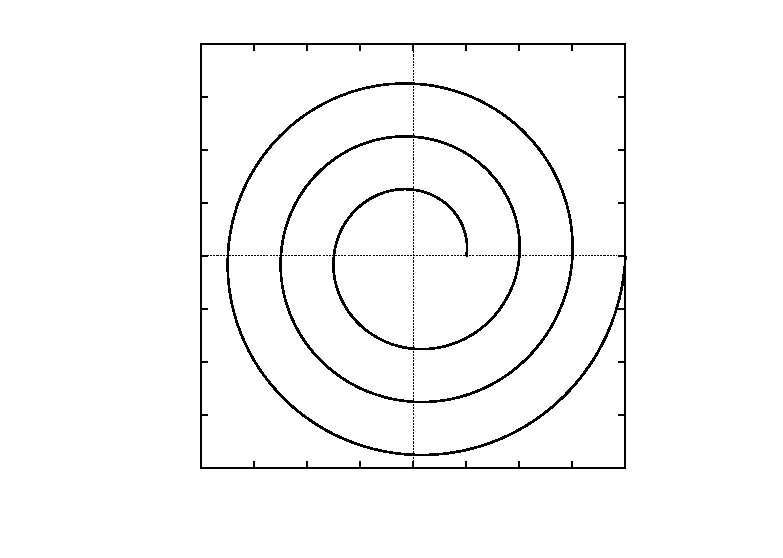
\includegraphics{spiral}}%
    \gplfronttext
  \end{picture}%
\endgroup
}}
\begin{verbatim}
set polar
set size square
set samples 2000
unset key
set zeroaxis
set xlabel "x"
set ylabel "y"
plot [0:6*pi] 1 + t/(2*pi)
\end{verbatim}\vspace{-30mm}
\picskip{0}
Note that when using the \texttt{set polar} command, Gnuplot will assume that the function being
plotted is $r$ as a function of $\theta$ (represented by the variable \texttt{t} in Gnuplot).
\end{exmp}\vspace{-1mm}
\divider
\newpage
\piccaption[]{\label{fig:polarconvert}}\parpic[r]{\begin{tikzpicture}[every node/.style={font=\small}]
 \draw [line width=0.5pt,-latex] (0.8,0) arc (0:55:0.8);
 \draw [black!60,line width=0.3pt,-latex] (-0.5,0) -- (2.2,0) node [right] {$x$};
 \draw [black!60,line width=0.3pt,-latex] (0,-0.5) -- (0,1.8) node [above] {$y$};
 \node [black!60,below left] at (0,0) {$O$};
 \node [right] at (30:0.4) {$\theta$};
 \draw [dashed] (1.1472,0) -- (1.1472,1.6383);
 \draw [snake=brace,segment amplitude=3mm] (1.3,1.6383) -- (1.3,0);
 \draw [snake=brace,segment amplitude=3mm] (1.1472,-0.1)-- (0,-0.1);
 \node[right] at (1.55,0.81915) {$y$};
 \node[below] at (0.5736,-0.35) {$x$};
 \draw [linecolor,line width=1.5pt] (0,0) -- (55:2) node[black,above left,midway] {$r$};
 \fill (55:2) circle (2pt) node[above right] {$(r,\theta)$} node[above left] {$(x,y)$};
\end{tikzpicture}}
Figure \ref{fig:polarconvert} shows how to convert between polar coordinates and Cartesian
coordinates. For a point with polar coordinates $(r,\theta)$ and Cartesian coordinates $(x,y)$:

\noindent\textbf{Polar to Cartesian:}
\begin{equation}\label{eqn:polartorect}
 \boxed{ x ~=~ r\,\cos\;\theta \qquad y ~=~ r\,\sin\;\theta }
\end{equation}

\noindent\textbf{Cartesian to Polar:}
\begin{equation}\label{eqn:recttopolar}
 \boxed{ r ~=~ \pm\;\sqrt{x^2 ~+~ y^2} \qquad \tan\;\theta ~=~ \frac{y}{x} ~~\text{if $x \ne 0$} }
\end{equation}\vspace{-2mm}
\picskip{0}
Note that in formula (\ref{eqn:recttopolar}), if $x = 0$ then $\theta = \pi/2$ or $\theta = 3\pi/2$.
Also, if $x \ne 0$ and $y \ne 0$ then the two possible solutions for $\theta$ in the equation
$\tan\;\theta ~=~ \frac{y}{x}$ are in opposite quadrants (for $0 \le \theta < 2\pi$). If the angle
$\theta$ is in the same quadrant as the point $(x,y)$, then $r = \sqrt{x^2 ~+~ y^2}$ (i.e. $r$ is
positive); otherwise $r = -\sqrt{x^2 ~+~ y^2}$ (i.e. $r$ is negative).

\begin{exmp}
Convert the following points from polar coordinates to Cartesian coordinates:\\
\textbf{(a)} $(2,30\Degrees)$; \textbf{(b)} $(3,3\pi/4)$; \textbf{(c)} $(-1,5\pi/3)$\vspace{1mm}
\par\noindent\textbf{Solution:} \textbf{(a)} Using formula (\ref{eqn:polartorect}) with $r=2$ and
$\theta = 30\Degrees$, we get:
\begin{displaymath}
 (x,y) ~=~ ( r\,\cos\;\theta, r\,\sin\;\theta) ~=~ (2\,\cos\;30\Degrees,2\,\sin\;30\Degrees) ~=~
 \left(2 \;\cdot\; \tfrac{\sqrt{3}}{2}, 2 \;\cdot\; \tfrac{1}{2} \right) \quad\Rightarrow\quad
 \boxed{(x,y) ~=~ \left( \sqrt{3},1 \right)}
\end{displaymath}
 \par\noindent\textbf{(b)} Using formula (\ref{eqn:polartorect}) with $r=3$ and
 $\theta = 3\pi/4$, we get:
\begin{displaymath}
 (x,y) ~=~ ( r\,\cos\;\theta, r\,\sin\;\theta) ~=~ \left( 3\,\cos\;\tfrac{3\pi}{4},3\,\sin\;\tfrac{3\pi}{4}
 \right) ~=~ \left(3 \;\cdot\; \tfrac{-1}{\sqrt{2}}, 3 \;\cdot\; \tfrac{1}{\sqrt{2}} \right)
 \quad\Rightarrow\quad \boxed{(x,y) ~=~ \left( \tfrac{-3}{\sqrt{2}},\tfrac{3}{\sqrt{2}} \right)}
\end{displaymath}
 \par\noindent\textbf{(c)} Using formula (\ref{eqn:polartorect}) with $r=-1$ and
 $\theta = 5\pi/3$, we get:
\begin{displaymath}
 (x,y) ~=~ ( r\,\cos\;\theta, r\,\sin\;\theta) ~=~ \left( -1\,\cos\;\tfrac{5\pi}{3},-1\,\sin\;\tfrac{5\pi}{3}
 \right) ~=~ \left(-1 \;\cdot\; \tfrac{1}{2},-1 \;\cdot\; \tfrac{-\sqrt{3}}{2} \right)
 \quad\Rightarrow\quad \boxed{(x,y) ~=~ \left( -\tfrac{1}{2},\tfrac{\sqrt{3}}{2} \right)}
\end{displaymath}
\end{exmp}
\begin{exmp}
Convert the following points from Cartesian coordinates to polar coordinates:\\
\textbf{(a)} $(3,4)$; \textbf{(b)} $(-5,-5)$\vspace{1mm}
\par\noindent\textbf{Solution:} \textbf{(a)} Using formula (\ref{eqn:recttopolar}) with $x=3$ and
$y=4$, we get:
\begin{displaymath}
 \tan\;\theta ~=~ \frac{y}{x} ~=~ \frac{4}{3} \quad\Rightarrow\quad \theta ~=~ 53.13\Degrees \quad
 \text{or}\quad \theta ~=~ 233.13\Degrees
\end{displaymath}
Since $\theta = 53.13\Degrees$ is in the same quadrant (QI) as the point $(x,y) = (3,4)$, we can
take\\$r ~=~ \sqrt{x^2 + y^2} = \sqrt{3^2 + 4^2} = 5$. Thus, $\boxed{(r,\theta) = (5,53.13\Degrees)}$~.

\noindent Note that if we had used $\theta = 233.13\Degrees$, then we would have $(r,\theta) =
(-5,233.13\Degrees)$.

\par\noindent\textbf{(b)}  Using formula (\ref{eqn:recttopolar}) with $x=-5$ and $y=-5$, we get:
\begin{displaymath}
 \tan\;\theta ~=~ \frac{y}{x} ~=~ \frac{-5}{-5} ~=~ 1 \quad\Rightarrow\quad \theta ~=~ 45\Degrees \quad
 \text{or}\quad \theta ~=~ 225\Degrees
\end{displaymath}
Since $\theta = 225\Degrees$ is in the same quadrant (QIII) as the point $(x,y) = (-5,-5)$, we can
take\\$r ~=~ \sqrt{x^2 + y^2} = \sqrt{(-5)^2 + (-5)^2} = 5\,\sqrt{2}$. Thus, $\boxed{(r,\theta) =
(5\,\sqrt{2},225\Degrees)}$~.

\noindent Note that if we had used $\theta = 45\Degrees$, then we would have $(r,\theta) =
(-5\,\sqrt{2},45\Degrees)$.
\end{exmp}
\begin{exmp}\label{exmp:polarcircle}
 Write the equation $x^2 + y^2 = 9$ in polar coordinates.\vspace{1mm}
 \par\noindent\textbf{Solution:} This is just the equation of a circle of radius $3$ centered at the
 origin. Since $r = \pm\sqrt{x^2 + y^2} = \pm\sqrt{9}$, in polar coordinates the equation can be written
 as simply $\boxed{r = 3}$~.
\end{exmp}
\begin{exmp}
 Write the equation $x^2 + (y-4)^2 = 16$ in polar coordinates.\vspace{1mm}
 \par\noindent\textbf{Solution:} This is the equation of a circle of radius $4$ centered at the point
 $(0,4)$. Expanding the equation, we get:
 \begin{align*}
  x^2 ~+~ (y-4)^2 ~&=~ 16\\
  x^2 ~+~ y^2 ~-~ 8y ~+~ 16 ~&=~ 16\\
  x^2 ~+~ y^2 ~&=~ 8y\\
  r^2 ~&=~ 8\,r\sin\;\theta\\
  r ~&=~ 8\,\sin\;\theta
 \end{align*}
 Why could we cancel $r$ from both sides in the last step? Because we know that the point $(0,0)$
 is on the circle, so canceling $r$ does not eliminate $r=0$ as a potential solution of the
 equation (since $\theta = 0\Degrees$ would make $r = 8\,\sin\;\theta = 8\,\sin\;0\Degrees = 0$). Thus,
 the equation is $\boxed{r = 8\,\sin\;\theta}$~.
\end{exmp}
\begin{exmp}
 Write the equation $y = x$ in polar coordinates.\vspace{1mm}
 \par\noindent\textbf{Solution:} This is the equation of a line through the origin. So when $x=0$, we
 know that $y=0$. When $x \ne 0$, we get:
 \begin{align*}
  y ~&=~ x\\
  \frac{y}{x} ~&=~ 1\\
  \tan\;\theta ~&=~ 1\\
  \theta ~&=~ 45\Degrees
 \end{align*}
Since there is no restriction on $r$, we could have $r=0$ and $\theta = 45\Degrees$, which would take care
of the case $x = 0$ (since then $(x,y) = (0,0)$, which is the same as $(r,\theta) = (0,45\Degrees))$. Thus,
the equation is $\boxed{\theta = 45\Degrees}$~.
\end{exmp}\vspace{-1mm}
\divider\vspace{-2mm}
\newpage
\begin{exmp}
 Prove that the distance $d$ between two points $(r_1 , \theta_1)$ and $(r_2 , \theta_2)$ in polar
 coordinates is
 \begin{equation}\label{eqn:polardist}
  d ~=~ \sqrt{r_1^2 ~+~ r_2^2 ~-~ 2r_1r_2\,\cos\;(\theta_1 - \theta_2)} ~~.
 \end{equation}
 \par\noindent\textbf{Solution:} The idea here is to use the distance formula in Cartesian coordinates,
 then convert that to polar coordinates. So write
 \begin{alignat*}{4}
  x_1 ~&=~ r_1 \,\cos\;\theta_1 \qquad& y_1 ~&=~ r_1 \,\sin\;\theta_1\\
  x_2 ~&=~ r_2 \,\cos\;\theta_2 \qquad& y_2 ~&=~ r_2 \,\sin\;\theta_2 ~.
 \end{alignat*}
 Then $(x_1,y_1)$ and $(x_2,y_2)$ are the Cartesian equivalents of $(r_1 , \theta_1)$ and $(r_2 , \theta_2)$,
 respectively. Thus, by the Cartesian coordinate distance formula,
 \begin{align*}
  d^2 ~&=~ (x_1 - x_2)^2 ~+~ (y_1 - y_2)^2\\
  &=~ (r_1 \,\cos\;\theta_1 - r_2 \,\cos\;\theta_2)^2 ~+~ (r_1 \,\sin\;\theta_1 - r_2 \,\sin\;\theta_2)^2\\
  &=~ r_1^2 \cos^2\;\theta_1 ~-~ 2r_1 r_2 \cos\;\theta_1~\cos\;\theta_2 ~+~ r_2^2 \cos^2\;\theta_2 ~+~
   r_1^2 \sin^2\;\theta_1 ~-~ 2r_1 r_2 \sin\;\theta_1~\sin\;\theta_2 ~+~ r_2^2 \sin^2\;\theta_2\\
  &=~ r_1^2 (\cos^2\;\theta_1 ~+~ \sin^2\;\theta_1) ~+~ r_2^2 (\cos^2\;\theta_2 ~+~ \sin^2\;\theta_2) ~-~
   2r_1 r_2 (\cos\;\theta_1~\cos\;\theta_2 ~+~ \sin\;\theta_1~\sin\;\theta_2)\\
  d^2 ~&=~ r_1^2 ~+~ r_2^2 ~-~ 2r_1r_2\,\cos\;(\theta_1 - \theta_2) ~,
 \end{align*}
 so the result follows by taking square roots of both sides.
\end{exmp}\vspace{-1mm}
\divider
\vspace{2mm}

In Example \ref{exmp:polarcircle} we saw that the equation $x^2 + y^2 = 9$ in Cartesian coordinates
could be expressed as $r = 3$ in polar coordinates. This equation describes a circle centered at the
origin, so the circle is symmetric about the origin. In general, polar coordinates are useful in
situations when there is symmetry about the origin (though there are other situations), which arise
in many physical applications.

\divider
\vspace{2mm}

\startexercises\label{sec6dot4}
\vspace{5mm}
{\small
\par\noindent For Exercises 1-5, convert the given point from polar coordinates to Cartesian
coordinates.
\begin{enumerate}[\bfseries 1.]
\begin{multicols}{5}
 \item $(6,210\Degrees)$
 \item $(-4,3\pi)$
 \item $(2,11\pi/6)$
 \item $(6,90\Degrees)$
 \item $(-1,405\Degrees)$
\end{multicols}
\suspend{enumerate}
For Exercises 6-10, convert the given point from Cartesian coordinates to polar coordinates.
\resume{enumerate}[{[\bfseries 1.]}]
\begin{multicols}{5}
 \item $(3,1)$
 \item $(-1,-3)$
 \item $(0,2)$
 \item $(4,-2)$
 \item $(-2,0)$
\end{multicols}
\suspend{enumerate}
For Exercises 11-18, write the given equation in polar coordinates.
\resume{enumerate}[{[\bfseries 1.]}]
\begin{multicols}{4}
 \item $(x-3)^2 + y^2 = 9$
 \item $y = -x$
 \item $x^2 - y^2 = 1$
 \item $3x^2 + 4y^2 - 6x = 9$
\end{multicols}
\item Graph the function $r = 1 + 2\,\cos\;\theta$ in polar coordinates.
\end{enumerate}}

\newpage
%Put the bibliography here
%\include{trigbook-biblio}
%Put appendices here
\fancyhf{}
\fancyhead[LE]{\tikzstyle{headbox} = [fill=headercolor,line width=0pt,rectangle,rounded corners]
 \begin{tikzpicture}
  \node [headbox] (box){%
   \begin{minipage}{\fminilength}%
     \sffamily{\bfseries\thepage\qquad \enskip\leftmark}
    \end{minipage}%
  };
 \end{tikzpicture}}
\fancyhead[LO]{\tikzstyle{headbox} = [fill=headercolor,line width=0pt,rectangle,rounded corners]
 \begin{tikzpicture}
  \node [headbox] (box){%
   \begin{minipage}{\fminilength}%
     \sffamily {}\hfill{\bfseries{\leftmark\qquad\thepage}}
    \end{minipage}%
  };
 \end{tikzpicture}}
\addchap[Appendix A:$\quad$Answers and Hints to Selected Exercises]{Appendix A}
\textsf{\textbf{\Large Answers and Hints to Selected Exercises}}
\begin{multicols}{2}
\section*{Chapter 1}
\subsection*{Section 1.1 (p. \pageref{sec1dot1})}
\textbf{1.} $115\Degrees$ \quad \textbf{3.} $A=52\Degrees$, $B=104\Degrees$ \quad
\textbf{5.} $45\Degrees$\\\textbf{7.} $A=9\Degrees$, $B=81\Degrees$ \quad
\textbf{8.} $0.011\Degrees$ and $89.989\Degrees$\\\textbf{9.} $25$ miles \quad \textbf{10.}
$111.8$ ft\\\textbf{15.} Hint: Are the opposite sides of the four-sided figure inside the circle
parallel?
\subsection*{Section 1.2 (p. \pageref{sec1dot2})}
\textbf{1.} $\sin\;A = 5/13$, $\cos\;A = 12/13$, $\tan\;A = 5/12$,\\
$\csc\;A = 13/5$, $\sec\;A = 13/12$, $\cot\;A = 12/5$;\\
$\sin\;B = 12/13$, $\cos\;B = 5/13$, $\tan\;B = 12/5$,\\
$\csc\;B = 13/12$, $\sec\;B = 13/5$, $\cot\;B = 5/12$\\
\textbf{3.} $\sin\;A = 7/25$, $\cos\;A = 24/25$, $\tan\;A = 7/24$,\\
$\csc\;A = 25/7$, $\sec\;A = 25/24$, $\cot\;A = 24/7$;\\
$\sin\;B = 24/25$, $\cos\;B = 7/25$, $\tan\;B = 24/7$,\\
$\csc\;B = 25/24$, $\sec\;B = 25/7$, $\cot\;B = 7/24$\\
\textbf{5.} $\sin\;A = 9/41$, $\cos\;A = 40/41$, $\tan\;A = 9/40$,\\
$\csc\;A = 41/9$, $\sec\;A = 41/40$, $\cot\;A = 40/9$;\\
$\sin\;B = 40/41$, $\cos\;B = 9/41$, $\tan\;B = 40/9$,\\
$\csc\;B = 41/40$, $\sec\;B = 41/9$, $\cot\;B = 9/40$\\
\textbf{7.} $\sin\;A = 1/\sqrt{10}$, $\cos\;A = 3/\sqrt{10}$, $\tan\;A = 1/3$,\\
$\csc\;A = \sqrt{10}$, $\sec\;A = \sqrt{10}/3$, $\cot\;A = 3$;\\
$\sin\;B = 3/\sqrt{10}$, $\cos\;B = 1/\sqrt{10}$, $\tan\;B = 3$,\\
$\csc\;B = \sqrt{10}/3$, $\sec\;B = \sqrt{10}$, $\cot\;B = 1/3$\\
\textbf{9.} $\sin\;A = 5/6$, $\cos\;A = \sqrt{11}/6$, $\tan\;A = 5/\sqrt{11}$,\\
$\csc\;A = 6/5$, $\sec\;A = 6/\sqrt{11}$, $\cot\;A = \sqrt{11}/5$;\\
$\sin\;B = \sqrt{11}/6$, $\cos\;B = 5/6$, $\tan\;B = \sqrt{11}/5$,\\
$\csc\;B = 6/\sqrt{11}$, $\sec\;B = 6/5$, $\cot\;B = 5/\sqrt{11}$\\
\textbf{11.} $\cos\;A = \sqrt{7}/4$, $\tan\;A = 3/\sqrt{7}$,
$\csc\;A = 4/3$, $\sec\;A = 4/\sqrt{7}$, $\cot\;A = \sqrt{7}/3$\\
\textbf{13.} $\sin\;A = \sqrt{6}/\sqrt{10}$, $\tan\;A = \sqrt{6}/2$,\\
$\csc\;A = \sqrt{10}/\sqrt{6}$, $\sec\;A = \sqrt{10}/2$, $\cot\;A = 2/\sqrt{6}$\\
\textbf{15.} $\sin\;A = 5/\sqrt{106}$, $\cos\;A = 9/\sqrt{106}$,\\
$\csc\;A = \sqrt{106}/5$, $\sec\;A = \sqrt{106}/9$, $\cot\;A = 9/5$\\
\textbf{17.} $\sin\;A = \sqrt{40}/7$, $\cos\;A = 3/7$,\\$\tan\;A = \sqrt{40}/3$,
$\csc\;A = 7/\sqrt{40}$, $\cot\;A = 3/\sqrt{40}$\\
\textbf{19.} $\cos\;3\Degrees$ \quad \textbf{21.} $\sin\;44\Degrees$ \quad
\textbf{23.} $\csc\;13\Degrees$\\
\textbf{25.} $\sin\;77\Degrees$ \quad
\textbf{27.} $\tan\;80\Degrees$ \quad \textbf{30.} Hint: Draw a right triangle with an acute
angle $A$.\\
\textbf{33.} Hint: Draw two right triangles whose hypotenuses are the same length.\\
\textbf{37.} \textbf{(a)} $\sqrt{13}/4$ \textbf{(b)} $4\sqrt{3}/\sqrt{13}$
\textbf{(c)} $3/\sqrt{13}$
\subsection*{Section 1.3 (p. \pageref{sec1dot3})}
\textbf{1.} $102.7$ ft \quad \textbf{3.} $241.1$ ft \quad \textbf{4.} $274$ ft \quad
\textbf{7.} $1062$ mi \quad \textbf{9.} $0.476$ in \quad \textbf{11.} $1.955$ in \quad
\textbf{13.} $0.4866$ in \quad \textbf{14.} Partial answer: $DE=a\;\cot\;\theta\;\,\cos^2\,\theta$
\quad \textbf{15.} $c=13$, $A=22.6\Degrees$, $B=67.4\Degrees$ \quad \textbf{17.} $a=0.28$, $c=2.02$,
$B=82\Degrees$ \quad \textbf{19.} $b=6.15$, $c=6.84$, $B=64\Degrees$\\
\textbf{21.} $a=6.15$, $c=6.84$, $A=64\Degrees$ \quad \textbf{23.} $a=\sqrt{2}$, $b=\sqrt{2}$,
$B=45\Degrees$ \quad \textbf{25.} \textbf{(a)} $0.944$ cm\\\textbf{(b)} $2.112$ cm \quad
\textbf{27.} \textbf{(a)} $\sqrt{3}\;a$ \quad \textbf{(b)} $35.26\Degrees$\\\textbf{29.} $1379.5$ ft $= 0.2613$ mi
\subsection*{Section 1.4 (p. \pageref{sec1dot4})}
\textbf{1.} QII \quad \textbf{3.} QIV \quad \textbf{5.} negative $y$-axis\\\textbf{7.} QIII
\quad \textbf{9.} QIV \quad \textbf{11.} QI, QIII \quad \textbf{13.} QI, QIV \quad
\textbf{15.} QI, QII \quad \textbf{17.} $43\Degrees$ \quad \textbf{19.} $54\Degrees$ \quad
\textbf{21.} $85\Degrees$ \quad \textbf{23.} $\sin\;\theta = \sqrt{3}/2$ and $\tan\;\theta =
-\sqrt{3}$; $\sin\;\theta = -\sqrt{3}/2$ and $\tan\;\theta = \sqrt{3}$\\\textbf{25.}
$\sin\;\theta = \sqrt{21}/5$ and $\tan\;\theta = \sqrt{21}/2$;\\$\sin\;\theta = -\sqrt{21}/5$ and
$\tan\;\theta = -\sqrt{21}/2$\\\textbf{27.} $\cos\;\theta = \sqrt{3}/2$ and $\tan\;\theta =
1/\sqrt{3}$;\\$\cos\;\theta = -\sqrt{3}/2$ and $\tan\;\theta = -1/\sqrt{3}$\\
\textbf{29.} $\cos\;\theta = \pm 1$ and $\tan\;\theta = 0$\\\textbf{31.} $\cos\;\theta = 0$
and $\tan\;\theta$ is undefined\\\textbf{33.} $\sin\;\theta = 1/\sqrt{5}$ and
$\cos\;\theta = -2/\sqrt{5}$;\\$\sin\;\theta = -1/\sqrt{5}$ and $\cos\;\theta =
2/\sqrt{5}$\\\textbf{35.} $\sin\;\theta = 5/13$ and
$\cos\;\theta = 12/13$;\\$\sin\;\theta = -5/13$ and $\cos\;\theta =
-12/13$ \quad \textbf{37.} No \quad \textbf{39.} No
\subsection*{Section 1.5 (p. \pageref{sec1dot5})}
\textbf{1.} \textbf{(a)} $328\Degrees$ \textbf{(b)} $148\Degrees$ \textbf{(c)} $212\Degrees$ \quad
\textbf{3.} \textbf{(a)} $248\Degrees$ \textbf{(b)} $68\Degrees$ \textbf{(c)} $292\Degrees$ \quad
\textbf{7.} $25\Degrees$, $155\Degrees$ \quad \textbf{9.} $65\Degrees$, $295\Degrees$ \quad
\textbf{11.} $38\Degrees$, $218\Degrees$ \quad \textbf{13.} $169\Degrees$,
$191\Degrees$\\\textbf{15.} $D=\left( \frac{ab^2}{a^2 + b^2}, \frac{a^2 b}{a^2 + b^2} \right)$
\section*{Chapter 2}
\subsection*{Section 2.1 (p. \pageref{sec2dot1})}
\textbf{1.} $b = 7.4$, $c = 15.1$, $C = 120\Degrees$ \quad \textbf{3.} $a = 9.7$, $b = 10.7$, $C =
95\Degrees$ \quad \textbf{5.} $b = 65.1$, $B = 136.5\Degrees$, $C = 18.5\Degrees$ \quad
\textbf{7.} No solution \quad \textbf{9.} $b = 24.9$, $B = 59.9\Degrees$, $C = 70.1\Degrees$;
$b = 9.9$, $B = 20.1\Degrees$, $C = 109.9\Degrees$ \quad \textbf{11.} $422$ mi/hr \quad \textbf{15.}
$5.66$ cm and $12.86$ cm \quad \textbf{16.} Hint: Think geometrically.
\subsection*{Section 2.2 (p. \pageref{sec2dot2})}
\textbf{1.} $a = 10.6$, $B = 40.9\Degrees$, $C = 79.1$ \quad \textbf{3.} $A = 47.9\Degrees$,
$b = 8.2$, $C = 72.1\Degrees$ \quad \textbf{5.} No solution \quad \textbf{7.} $4.13$ and $8.91$ cm
\quad \textbf{9.} $50.5\Degrees$, $59\Degrees$, $70.5\Degrees$\\\textbf{11.} $7$ cm \quad
\textbf{15.} Hints: One of the angles in the formulas is a right angle; also, use the definition of
cosine.
\subsection*{Section 2.3 (p. \pageref{sec2dot3})}
\textbf{1.} $A = 79.1\Degrees$, $B = 40.9\Degrees$, $c = 10.6$ \quad \textbf{3.} $A = 47.9\Degrees$,
$b = 8.2$, $C = 72.1\Degrees$ \quad \textbf{5.} No \quad \textbf{6.} Yes \quad \textbf{11.} Hint:
Think of Exercise 10.
\subsection*{Section 2.4 (p. \pageref{sec2dot4})}
\textbf{1.} $22.55$ \quad \textbf{3.} $9.21$ \quad \textbf{5.} $\frac{3}{4}\sqrt{15}
\approx 2.905$\\\textbf{7.} $12.21$ \quad \textbf{9.} Hints: The diagonals break the quadrilateral
into four triangles; also, consider formulas (\ref{eqn:areacase1a})-(\ref{eqn:areacase1c}).
\subsection*{Section 2.5 (p. \pageref{sec2dot5})}
\textbf{1.} $R = 2.63$, $r = 0.69$ \quad \textbf{3.} $R = 3.51$, $r = 1.36$ \quad
\textbf{5.} $R = 24.18$, $r = 1.12$ \quad \textbf{12.} \textbf{(c)} Twice as large
\textbf{(d)} Hint: Bisect each angle.
\section*{Chapter 3}
\subsection*{Section 3.1 (p. \pageref{sec3dot1})}
\textbf{1.} $\theta = 270\Degrees$ \quad \textbf{3.} Hint: See Example \ref{exmp:elimtheta}. \quad
\textbf{19.} $\tan\;\theta = \pm\,\sin\;\theta / \sqrt{1 - \sin^2 \;\theta} =
\pm\,\sqrt{1 - \cos^2 \;\theta} / \cos\;\theta$
\subsection*{Section 3.2 (p. \pageref{sec3dot2})}
\textbf{3.} $\sin\;(A+B) = \frac{1020}{1189}$, $\cos\;(A+B) = -\frac{611}{1189}$,
$\tan\;(A+B) = -\frac{1020}{611}$ \quad \textbf{4.} $(\sqrt{6} + \sqrt{2})/4$\\
\textbf{5.} $2 - \sqrt{3}$ \quad \textbf{15.} Hint: For $a \ne 0$ and $b \ne 0$, draw a right
triangle with legs of lengths $a$ and $b$.
\subsection*{Section 3.3 (p. \pageref{sec3dot3})}
\textbf{9.} Hint: Is $\sin\;A + \cos\;A$ always positive? \textbf{11.} $1/2$
\subsection*{Section 3.4 (p. \pageref{sec3dot4})}
\textbf{13.} Hint: One way to do this is with the Law of Tangents. Another way is with the Law of
Sines.
\section*{Chapter 4}
\subsection*{Section 4.1 (p. \pageref{sec4dot1})}
\textbf{1.} $\pi/45$ \quad \textbf{3.} $13\pi/18$ \quad \textbf{5.} $-3\pi/5$ \quad
\textbf{7.} $36\Degrees$ \quad \textbf{9.} $174\Degrees$
\subsection*{Section 4.2 (p. \pageref{sec4dot2})}
\textbf{1.} $9.6$ cm \quad \textbf{3.} $11\pi$ in \quad \textbf{5.} $54.94$ in\\
\textbf{7.} $12.86$ ft \quad \textbf{8.} $34.18$ \quad \textbf{9.} $38.26$\\
\textbf{11.} $3.392$ and $9.174$ \quad \textbf{12.} $3.105828541$
\subsection*{Section 4.3 (p. \pageref{sec4dot3})}
\textbf{1.} $1.512~\text{cm}^2$ \quad \textbf{3.} $24.5~\text{m}^2$ \quad
\textbf{5.} $269.1~\text{cm}^2$ \quad \textbf{7.} $5~\text{cm}^2$ \quad
\textbf{9.} $\pi/2~\text{cm}^2$ \quad \textbf{11.} $0.017~\text{cm}^2$ \quad
\textbf{13.} $21.46$ \quad \textbf{15.} $48.17$ \quad \textbf{17.} $0.522~\text{m}^2$\\
\textbf{19.} Sector area is quadrupled, arc length is doubled.
\subsection*{Section 4.4 (p. \pageref{sec4dot4})}
\textbf{1.} $\nu=6$ m/sec, $\omega=1.5$ rad/sec\\
\textbf{3.} $\nu=6.6$ m/sec, $\omega=0.94$ rad/sec\\
\textbf{5.} $\nu=3.75$ m/sec, $\omega=1.875$ rad/sec\\
\textbf{7.} $3.375$ rad \quad \textbf{9.} $32$ rpm and $21.33$ rpm\\
\textbf{11.} $40.84$ in/sec
\section*{Chapter 5}
\subsection*{Section 5.1 (p. \pageref{sec5dot1})}
\textbf{13.} Partial answer: $\sec\;\theta = OQ$
\subsection*{Section 5.2 (p. \pageref{sec5dot2})}
\textbf{1.} amplitude $= 3$, period $= 2$, phase shift = $0$ \quad
\textbf{3.} amplitude $= 1$, period $= 2\pi/5$, phase shift = $-3/5$ \quad
\textbf{5.} amplitude $= 1$, period $= 2\pi/5$, phase shift = $-\pi/5$ \quad
\textbf{7.} amplitude $= 1$, period $= \pi$, phase shift = $3\pi/2$\\
\textbf{9.} amplitude undefined, period $= \pi/2$, phase shift = $3\pi/2$ \quad
\textbf{11.} amplitude undefined, period $= \pi$, phase shift = $1/2$\\
\textbf{13.} max. at $x=\pm\,\sqrt{\pi/2}$, $\pm\,\sqrt{5\pi/2}$, $\pm\,\sqrt{9\pi/2}$, $...$\\
min. at $x=\pm\,\sqrt{3\pi/2}$, $\pm\,\sqrt{7\pi/2}$, $\pm\,\sqrt{11\pi/2}$, $...$\\
\textbf{15.} amplitude $= 0.5$, period $= \pi$ \quad \textbf{17.} out of phase \quad
\textbf{18.} in phase \quad \textbf{19.} amplitude $= \sqrt{34}$, period $= 2$ \quad
\textbf{21.} amplitude $= 2\,\sqrt{2}$, period $= 2\pi$ \quad
\textbf{23.} $2\pi$ \quad \textbf{25.} $6$ \quad \textbf{27.} amplitude envelope: $y=\pm\,x^2$ \quad
\textbf{29.} No
\subsection*{Section 5.3 (p. \pageref{sec5dot3})}
\textbf{1.} $\pi/4$ \quad \textbf{3.} $0$ \quad \textbf{5.} $\pi$ \quad \textbf{7.} $\pi/2$ \quad
\textbf{9.} $0$\\\textbf{11.} $-\pi/3$ \quad \textbf{13.} $\pi/7$ \quad \textbf{15.} $4\pi/5$
\quad \textbf{17.} $\pi/6$\\\textbf{19.} $-\pi/9$ \quad \textbf{21.} $12/13$ \quad
\textbf{23.} $\pi/2$ \quad \textbf{25.} $\pi/2$
\section*{Chapter 6}
\subsection*{Section 6.1 (p. \pageref{sec6dot1})}
\textbf{1.} $\frac{3\pi}{4} + \pi k$ \quad \textbf{3.} $\frac{3\pi}{10} + \frac{2\pi k}{5}$ \quad
\textbf{5.} $\pm\,\frac{\pi}{6} + \pi k$\\\textbf{7.} $-0.821 + 2\pi k$, $3.963 + 2\pi k$ \quad
\textbf{9.} $\frac{\pi}{4} + \pi k$\\\textbf{11.} $\frac{2\pi k}{3}$
\subsection*{Section 6.2 (p. \pageref{sec6dot2})}
\textbf{1.} $x=1.89549426703398093962$
\subsection*{Section 6.3 (p. \pageref{sec6dot3})}
\textbf{1.} $-1+i$ \quad \textbf{3.} $-13i$ \quad \textbf{5.} $-1-i$ \quad \textbf{7.} $i$\\
\textbf{9.} $-i$ \quad \textbf{11.} $i$ \quad \textbf{13.} $-i$ \quad \textbf{15.} $i$\\
\textbf{17.} Let $z=a+bi$. Then $\overline{z}=a-bi$, so $\overline{\left(\overline{z}\right)} =
\overline{a-bi}=a+bi=z$. \quad \textbf{23.} Hint: Use Exercise 20. \quad
\textbf{25.} $\sqrt{13}\,\text{cis}\;56.3\Degrees$ \quad
\textbf{27.} $\sqrt{2}\,\text{cis}\;315\Degrees$ \quad \textbf{29.} $\text{cis}\;0\Degrees$ \quad
\textbf{33.} $81\,\text{cis}\;56\Degrees$ \quad \textbf{35.} $1.5\,\text{cis}\;253\Degrees$ \quad
\textbf{37.} $\sqrt[6]{2}\,\text{cis}\;15\Degrees$, $\sqrt[6]{2}\,\text{cis}\;135\Degrees$,
$\sqrt[6]{2}\,\text{cis}\;255\Degrees$\\\textbf{39.} $\frac{1}{2} + \frac{\sqrt{3}}{2}\,i$,
$-1$, $\frac{1}{2} - \frac{\sqrt{3}}{2}\,i$ \quad \textbf{41.} $\text{cis}\;36\Degrees$,
$\text{cis}\;108\Degrees$, $\text{cis}\;180\Degrees$, $\text{cis}\;252\Degrees$,
$\text{cis}\;324\Degrees$
\subsection*{Section 6.4 (p. \pageref{sec6dot4})}
\textbf{1.} $(-3\sqrt{3},-3)$ \quad \textbf{3.} $(\sqrt{3},-1)$\\
\textbf{5.} $(-1/\sqrt{2},-1/\sqrt{2})$ \quad \textbf{7.} $(\sqrt{10},251.6\Degrees)$\\
\textbf{9.} $(2\sqrt{5},333.4\Degrees)$ \quad \textbf{11.} $r = 6\,\cos\;\theta$\\
\textbf{13.} $r^2 \,\cos\;2\theta = 1$ \quad \textbf{14.} $r = 3/(2 - \cos\;\theta)$
\end{multicols}

\addchap[Appendix B:$\quad$Graphing with Gnuplot]{Appendix B}
\textsf{\textbf{\Large Graphing with Gnuplot}}\vspace{4mm}

Gnuplot is a free, open-source software package for producing a variety of graphs. Versions are
available for many operating systems. Below is a very brief tutorial on how to use Gnuplot to graph
trigonometric functions.\vspace{4mm}

\par\noindent\textbf{\textsf{INSTALLATION}}
\begin{enumerate}
 \item Go to \url{http://www.gnuplot.info/download.html} and follow the links to download the latest
  version for your operating system. For Windows, you should download the setup file with a name
  such as \path{gp460-win32-setup.exe}, which is
  version 4.6.0. All the examples discussed here will assume at least version 4.6.0, though they
  should work with earlier 4.x versions.
 \item Install the downloaded file. For example, in Windows you would run the setup file you
  downloaded in Step 1, which installs Gnuplot in the
  \texttt{C:\symbol{92}Program Files\symbol{92}gnuplot} folder by default.
  You can accept the defaults during installation, though you
  should select the  ``Create a desktop icon'' option in the \textbf{Select Additional Tasks}
  screen.
 \item (Optional) Read the documentation at \url{http://gnuplot.info/documentation.html}.
\end{enumerate}

\par\noindent\textbf{\textsf{RUNNING GNUPLOT}}
\begin{enumerate}
 \item In Windows, run \textbf{\path{wgnuplot.exe}} from the \path{bin} folder where you
  installed Gnuplot (the default location is
  \texttt{C:\symbol{92}Program Files\symbol{92}gnuplot\symbol{92}bin\symbol{92}wgnuplot.exe}),
  or double-click the desktop icon if you selected that option during the installation.
  In Linux, just type \textbf{\path{gnuplot}} in a terminal window.
 \item You should now get a Gnuplot terminal with a \textbf{\path{gnuplot>}} command prompt. In
  Windows this will appear in a new window, as shown in the picture on the next page.
  In Linux it will appear in the terminal window
  where the \textbf{\path{gnuplot}} command was
  run. For Windows, if the font is unreadable you can change it by right-clicking on the text part
  of the Gnuplot window
  and selecting the ``Choose Font..'' option. For example, the font ``Courier'', style ``Regular'',
  size ``12'' is usually a
  good choice (that choice can be saved for future sessions by right-clicking in the Gnuplot window
  again and selecting the option to update wgnuplot.ini).
 \item At the \textbf{\path{gnuplot>}} command prompt you can now run graphing commands, which we
  will now describe.
\end{enumerate}
\newpage
\begin{figure}[h]
 \begin{center}
  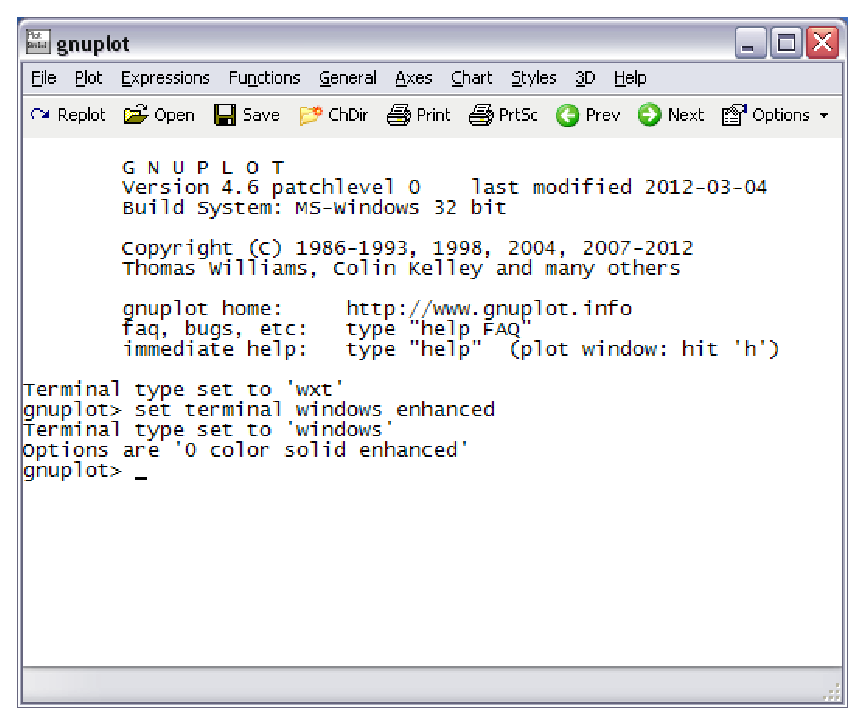
\includegraphics{wgnuplot.eps}
 \end{center}
\end{figure}

\par\noindent\textbf{\textsf{GRAPHING FUNCTIONS}}\vspace{2mm}\\
The usual way to create graphs in Gnuplot is with the \textbf{\path{plot}} command:
\begin{displaymath}
 \texttt{plot \emph{<range> <comma-separated list of functions>}}
\end{displaymath}
For a function $y=f(x)$, \texttt{\emph{<range>}} is the range of $x$ values (and optionally the
range of $y$ values) over which to plot. To specify an $x$ range, use an expression of the form
\symbol{91}$a:b$\symbol{93}, for some numbers $a<b$. This will cause the graph to
be plotted for $a\le x\le b$.\vspace{2mm}

To specify an $x$ range and a $y$ range, use an expression of the form
\symbol{91}$a:b$\symbol{93}\symbol{91}$c:d$\symbol{93}, for some numbers $a<b$ and $c<d$. This will
cause the graph to be plotted for $a\le x\le b$ and $c\le y \le d$.\vspace{2mm}

\par\noindent Function definitions use the $x$ variable in combination with mathematical operators,
listed below:\vspace{1mm}

\begin{center}
\begin{tabular}{@{} | c | c | c | c | @{}}
 \hline \textbf{Symbol} & \textbf{Operation} & \textbf{Example} & \textbf{Result}\\
 \hline $+$ & Addition & $2 + 3$ & $5$\\
 \hline $-$ & Subtraction & $3 - 2$ & $1$\\
 \hline * & Multiplication & $2$*$3$ & $6$\\
 \hline $/$ & Division & $4/2$ & $2$\\
 \hline ** & Power & $2$**$3$ & $2^3 = 8$\\
 \hline exp($x$) & $e^x$ & exp($2$) & $e^2$\\
 \hline log($x$) & $\ln x$ & log($2$) & $\ln 2$\\
 \hline sin($x$) & $\sin x$ & sin(pi/$2$) & $1$\\
 \hline cos($x$) & $\cos x$ & cos(pi) & $-1$\\
 \hline tan($x$) & $\tan x$ & tan(pi/$4$) & $1$\\\hline
\end{tabular}\end{center}

Note that we use the special keyword ``pi'' to denote the value of $\pi$.

\vspace{2mm}
\hrule width \textwidth height 0.5pt\vspace{2mm}
\par\noindent \emph{\textbf{Example B.1.}}
 To graph the function $y=\sin\;x$ from $x=0$ to $x=2\pi$, type this at the
 \textbf{\path{gnuplot>}} prompt:
 \begin{displaymath}
  \texttt{plot \symbol{91}0:2*pi\symbol{93} sin(x)}
 \end{displaymath}
 The result is shown below:
 
\begin{figure}[h]
 \begin{center}
  % GNUPLOT: LaTeX picture with Postscript
\begingroup
\footnotesize
  \makeatletter
  \providecommand\color[2][]{%
    \GenericError{(gnuplot) \space\space\space\@spaces}{%
      Package color not loaded in conjunction with
      terminal option `colourtext'%
    }{See the gnuplot documentation for explanation.%
    }{Either use 'blacktext' in gnuplot or load the package
      color.sty in LaTeX.}%
    \renewcommand\color[2][]{}%
  }%
  \providecommand\includegraphics[2][]{%
    \GenericError{(gnuplot) \space\space\space\@spaces}{%
      Package graphicx or graphics not loaded%
    }{See the gnuplot documentation for explanation.%
    }{The gnuplot epslatex terminal needs graphicx.sty or graphics.sty.}%
    \renewcommand\includegraphics[2][]{}%
  }%
  \providecommand\rotatebox[2]{#2}%
  \@ifundefined{ifGPcolor}{%
    \newif\ifGPcolor
    \GPcolortrue
  }{}%
  \@ifundefined{ifGPblacktext}{%
    \newif\ifGPblacktext
    \GPblacktexttrue
  }{}%
  % define a \g@addto@macro without @ in the name:
  \let\gplgaddtomacro\g@addto@macro
  % define empty templates for all commands taking text:
  \gdef\gplbacktext{}%
  \gdef\gplfronttext{}%
  \makeatother
  \ifGPblacktext
    % no textcolor at all
    \def\colorrgb#1{}%
    \def\colorgray#1{}%
  \else
    % gray or color?
    \ifGPcolor
      \def\colorrgb#1{\color[rgb]{#1}}%
      \def\colorgray#1{\color[gray]{#1}}%
      \expandafter\def\csname LTw\endcsname{\color{white}}%
      \expandafter\def\csname LTb\endcsname{\color{black}}%
      \expandafter\def\csname LTa\endcsname{\color{black}}%
      \expandafter\def\csname LT0\endcsname{\color[rgb]{1,0,0}}%
      \expandafter\def\csname LT1\endcsname{\color[rgb]{0,1,0}}%
      \expandafter\def\csname LT2\endcsname{\color[rgb]{0,0,1}}%
      \expandafter\def\csname LT3\endcsname{\color[rgb]{1,0,1}}%
      \expandafter\def\csname LT4\endcsname{\color[rgb]{0,1,1}}%
      \expandafter\def\csname LT5\endcsname{\color[rgb]{1,1,0}}%
      \expandafter\def\csname LT6\endcsname{\color[rgb]{0,0,0}}%
      \expandafter\def\csname LT7\endcsname{\color[rgb]{1,0.3,0}}%
      \expandafter\def\csname LT8\endcsname{\color[rgb]{0.5,0.5,0.5}}%
    \else
      % gray
      \def\colorrgb#1{\color{black}}%
      \def\colorgray#1{\color[gray]{#1}}%
      \expandafter\def\csname LTw\endcsname{\color{white}}%
      \expandafter\def\csname LTb\endcsname{\color{black}}%
      \expandafter\def\csname LTa\endcsname{\color{black}}%
      \expandafter\def\csname LT0\endcsname{\color{black}}%
      \expandafter\def\csname LT1\endcsname{\color{black}}%
      \expandafter\def\csname LT2\endcsname{\color{black}}%
      \expandafter\def\csname LT3\endcsname{\color{black}}%
      \expandafter\def\csname LT4\endcsname{\color{black}}%
      \expandafter\def\csname LT5\endcsname{\color{black}}%
      \expandafter\def\csname LT6\endcsname{\color{black}}%
      \expandafter\def\csname LT7\endcsname{\color{black}}%
      \expandafter\def\csname LT8\endcsname{\color{black}}%
    \fi
  \fi
  \setlength{\unitlength}{0.0500bp}%
  \begin{picture}(7200.00,5040.00)%
    \gplgaddtomacro\gplbacktext{%
      \csname LTb\endcsname%
      \put(726,440){\makebox(0,0)[r]{\strut{}-1}}%
      \put(726,873){\makebox(0,0)[r]{\strut{}-0.8}}%
      \put(726,1307){\makebox(0,0)[r]{\strut{}-0.6}}%
      \put(726,1740){\makebox(0,0)[r]{\strut{}-0.4}}%
      \put(726,2174){\makebox(0,0)[r]{\strut{}-0.2}}%
      \put(726,2608){\makebox(0,0)[r]{\strut{} 0}}%
      \put(726,3041){\makebox(0,0)[r]{\strut{} 0.2}}%
      \put(726,3475){\makebox(0,0)[r]{\strut{} 0.4}}%
      \put(726,3908){\makebox(0,0)[r]{\strut{} 0.6}}%
      \put(726,4342){\makebox(0,0)[r]{\strut{} 0.8}}%
      \put(726,4775){\makebox(0,0)[r]{\strut{} 1}}%
      \put(858,220){\makebox(0,0){\strut{} 0}}%
      \put(1804,220){\makebox(0,0){\strut{} 1}}%
      \put(2750,220){\makebox(0,0){\strut{} 2}}%
      \put(3697,220){\makebox(0,0){\strut{} 3}}%
      \put(4643,220){\makebox(0,0){\strut{} 4}}%
      \put(5589,220){\makebox(0,0){\strut{} 5}}%
      \put(6535,220){\makebox(0,0){\strut{} 6}}%
    }%
    \gplgaddtomacro\gplfronttext{%
      \csname LTb\endcsname%
      \put(5816,4602){\makebox(0,0)[r]{\strut{}$\sin(x)$}}%
    }%
    \gplbacktext
    \put(0,0){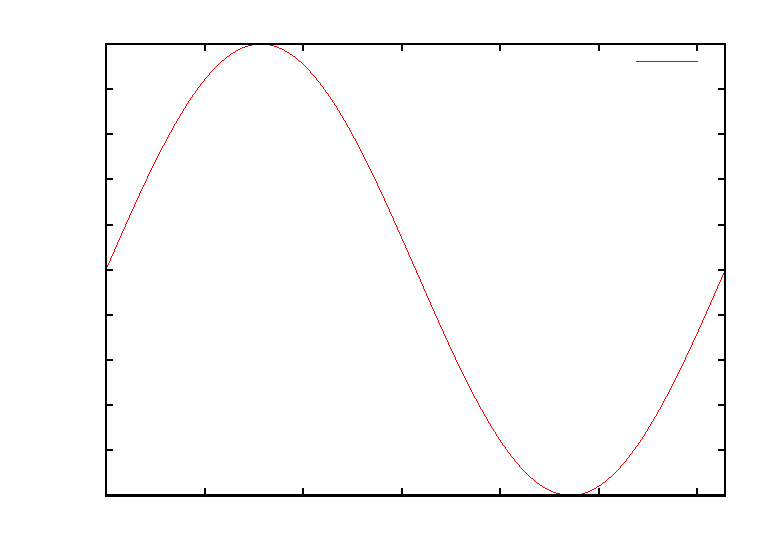
\includegraphics{sine}}%
    \gplfronttext
  \end{picture}%
\endgroup

 \end{center}
\end{figure}

Notice that the $x$-axis is labeled with integers. To get the $x$-axis labels with fractions of
$\pi$, you need to modify the \texttt{terminal} setting. In Windows, you would do this:
\begin{displaymath}
 \texttt{set terminal windows enhanced}
\end{displaymath}
In Linux you would do this:
\begin{displaymath}
 \texttt{set terminal wxt enhanced}
\end{displaymath}
You can then (provided the Symbol font is installed, which it usually is) set the $x$-axis to have
multiples of $\pi/2$ from $0$ to $2\pi$ as labels with this command (all on one line):
\begin{gather*}
 \texttt{set xtics ('0' 0,'\{/Symbol p\}/2' pi/2,'\{/Symbol p\}' pi,'3\{/Symbol p\}/2' 3*pi/2,}\\
 \texttt{'2\{/Symbol p\}' 2*pi)}
\end{gather*}
In the above example,
 to also plot the function $y=\cos\;2x + \sin\;3x$ on the same graph, put a comma after the first
 function then append the new function:
 \begin{displaymath}
  \texttt{plot \symbol{91}0:2*pi\symbol{93} sin(x), cos(2*x) + sin(3*x)}
 \end{displaymath}
By default, the $x$-axis is not shown in the graph. To display it, use this command
\emph{before} the \textbf{\path{plot}} command:
\begin{displaymath}
 \texttt{set zeroaxis}
\end{displaymath}
Also, to label the axes, use these commands:
\begin{gather*}
 \texttt{set xlabel "x"}\\\texttt{set ylabel "y"}
\end{gather*}
The default sample size for plots is $100$ units, which can result in jagged edges if the curve
is complicated. To get a smoother curve, increase the
sample size (to, say, $1000$) like this:
\begin{displaymath}
 \texttt{set samples 1000}
\end{displaymath}
Putting all this together, we get the following graph:

\begin{figure}[H]
 \begin{center}
  % GNUPLOT: LaTeX picture with Postscript
\begingroup
\footnotesize
  \makeatletter
  \providecommand\color[2][]{%
    \GenericError{(gnuplot) \space\space\space\@spaces}{%
      Package color not loaded in conjunction with
      terminal option `colourtext'%
    }{See the gnuplot documentation for explanation.%
    }{Either use 'blacktext' in gnuplot or load the package
      color.sty in LaTeX.}%
    \renewcommand\color[2][]{}%
  }%
  \providecommand\includegraphics[2][]{%
    \GenericError{(gnuplot) \space\space\space\@spaces}{%
      Package graphicx or graphics not loaded%
    }{See the gnuplot documentation for explanation.%
    }{The gnuplot epslatex terminal needs graphicx.sty or graphics.sty.}%
    \renewcommand\includegraphics[2][]{}%
  }%
  \providecommand\rotatebox[2]{#2}%
  \@ifundefined{ifGPcolor}{%
    \newif\ifGPcolor
    \GPcolortrue
  }{}%
  \@ifundefined{ifGPblacktext}{%
    \newif\ifGPblacktext
    \GPblacktexttrue
  }{}%
  % define a \g@addto@macro without @ in the name:
  \let\gplgaddtomacro\g@addto@macro
  % define empty templates for all commands taking text:
  \gdef\gplbacktext{}%
  \gdef\gplfronttext{}%
  \makeatother
  \ifGPblacktext
    % no textcolor at all
    \def\colorrgb#1{}%
    \def\colorgray#1{}%
  \else
    % gray or color?
    \ifGPcolor
      \def\colorrgb#1{\color[rgb]{#1}}%
      \def\colorgray#1{\color[gray]{#1}}%
      \expandafter\def\csname LTw\endcsname{\color{white}}%
      \expandafter\def\csname LTb\endcsname{\color{black}}%
      \expandafter\def\csname LTa\endcsname{\color{black}}%
      \expandafter\def\csname LT0\endcsname{\color[rgb]{1,0,0}}%
      \expandafter\def\csname LT1\endcsname{\color[rgb]{0,1,0}}%
      \expandafter\def\csname LT2\endcsname{\color[rgb]{0,0,1}}%
      \expandafter\def\csname LT3\endcsname{\color[rgb]{1,0,1}}%
      \expandafter\def\csname LT4\endcsname{\color[rgb]{0,1,1}}%
      \expandafter\def\csname LT5\endcsname{\color[rgb]{1,1,0}}%
      \expandafter\def\csname LT6\endcsname{\color[rgb]{0,0,0}}%
      \expandafter\def\csname LT7\endcsname{\color[rgb]{1,0.3,0}}%
      \expandafter\def\csname LT8\endcsname{\color[rgb]{0.5,0.5,0.5}}%
    \else
      % gray
      \def\colorrgb#1{\color{black}}%
      \def\colorgray#1{\color[gray]{#1}}%
      \expandafter\def\csname LTw\endcsname{\color{white}}%
      \expandafter\def\csname LTb\endcsname{\color{black}}%
      \expandafter\def\csname LTa\endcsname{\color{black}}%
      \expandafter\def\csname LT0\endcsname{\color{black}}%
      \expandafter\def\csname LT1\endcsname{\color{black}}%
      \expandafter\def\csname LT2\endcsname{\color{black}}%
      \expandafter\def\csname LT3\endcsname{\color{black}}%
      \expandafter\def\csname LT4\endcsname{\color{black}}%
      \expandafter\def\csname LT5\endcsname{\color{black}}%
      \expandafter\def\csname LT6\endcsname{\color{black}}%
      \expandafter\def\csname LT7\endcsname{\color{black}}%
      \expandafter\def\csname LT8\endcsname{\color{black}}%
    \fi
  \fi
  \setlength{\unitlength}{0.0500bp}%
  \begin{picture}(7200.00,5040.00)%
    \gplgaddtomacro\gplbacktext{%
      \csname LTb\endcsname%
      \put(946,704){\makebox(0,0)[r]{\strut{}-2}}%
      \put(946,1213){\makebox(0,0)[r]{\strut{}-1.5}}%
      \put(946,1722){\makebox(0,0)[r]{\strut{}-1}}%
      \put(946,2231){\makebox(0,0)[r]{\strut{}-0.5}}%
      \put(946,2740){\makebox(0,0)[r]{\strut{} 0}}%
      \put(946,3248){\makebox(0,0)[r]{\strut{} 0.5}}%
      \put(946,3757){\makebox(0,0)[r]{\strut{} 1}}%
      \put(946,4266){\makebox(0,0)[r]{\strut{} 1.5}}%
      \put(946,4775){\makebox(0,0)[r]{\strut{} 2}}%
      \put(1078,484){\makebox(0,0){\strut{}$0$}}%
      \put(2509,484){\makebox(0,0){\strut{}$\pi/2$}}%
      \put(3941,484){\makebox(0,0){\strut{}$\pi$}}%
      \put(5372,484){\makebox(0,0){\strut{}$3\pi/2$}}%
      \put(6803,484){\makebox(0,0){\strut{}$2\pi$}}%
      \csname LTb\endcsname%
      \put(176,2739){\rotatebox{-270}{\makebox(0,0){\strut{}$y$}}}%
      \put(3940,154){\makebox(0,0){\strut{}$x$}}%
    }%
    \gplgaddtomacro\gplfronttext{%
      \csname LTb\endcsname%
      \put(5816,4602){\makebox(0,0)[r]{\strut{}$\sin(x)$}}%
      \csname LTb\endcsname%
      \put(5816,4382){\makebox(0,0)[r]{\strut{}$\cos(2*x) + \sin(3*x)$}}%
    }%
    \gplbacktext
    \put(0,0){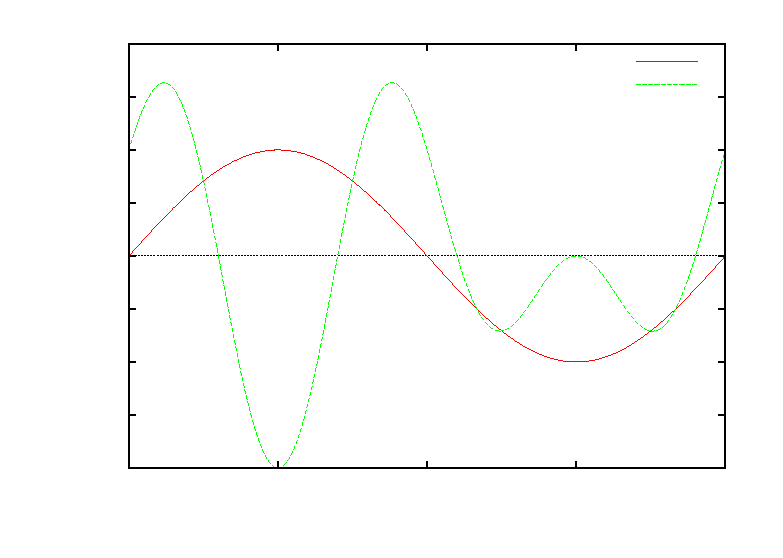
\includegraphics{tutorial}}%
    \gplfronttext
  \end{picture}%
\endgroup

 \end{center}
\end{figure}\vspace{-4mm}
\lineacross
\vspace{3mm}

\par\noindent\textbf{\textsf{PRINTING AND SAVING}}\vspace{2mm}\\
In Windows, if you are using the \texttt{windows enhanced} terminal then to print a graph from
Gnuplot click on the printer icon in the menubar of the graph's window. If you are using the
default \texttt{wxt} terminal then select \textbf{Print} near the top of the main Gnuplot window
and enter \path{png} in the \emph{Terminal type?} textfield, then hit OK to get the Print Setup
dialog.

In Windows, to save a graph, say, as a PNG file, go to the File menu on the main Gnuplot menubar,
select ``Output Device ...'', and enter \path{png} in the \emph{Terminal type?} textfield, hit OK. Then, in the
File menu again, select the ``Output ...'' option and enter a filename (say, graph.png) in the \emph{Output
filename?} textfield, hit OK. Now run your plot command again and the file will be saved in the
current directory, usually in your \texttt{My Documents} folder (it can also be found by
selecting the ``show Current Directory'' option in the File menu).\\

\par\noindent In Linux, to save the graph as a file called graph.png run the following
commands:\vspace{2mm}

\begin{tabular}{l @{}}
\texttt{set terminal png}\\
\texttt{set output 'graph.png'}
\end{tabular}\vspace{2mm}

\par\noindent and then run your plot command. There are many terminal types (which determine the output format). Run
the command \textbf{\texttt{set terminal}} to see all the possible types. In Linux, the \textbf{postscript} terminal type is
popular, since the print quality is high and there are many PostScript viewers available.
\vspace{2mm}

\par\noindent To quit Gnuplot, type \textbf{\path{quit}} at the \textbf{\path{gnuplot>}} command prompt.

\newpage
%Put the GNU FDL here
\addchap{GNU Free Documentation License}

 \begin{center}

       Version 1.3, 3 November 2008


 Copyright \copyright{} 2000, 2001, 2002, 2007, 2008  Free Software Foundation, Inc.
 
 \bigskip
 
     \url{<http://fsf.org/>}
  
 \bigskip
 
 Everyone is permitted to copy and distribute verbatim copies
 of this license document, but changing it is not allowed.
\end{center}


\begin{center}
{\bf\large \textsf{Preamble}}
\end{center}

The purpose of this License is to make a manual, textbook, or other
functional and useful document ``free'' in the sense of freedom: to
assure everyone the effective freedom to copy and redistribute it,
with or without modifying it, either commercially or noncommercially.
Secondarily, this License preserves for the author and publisher a way
to get credit for their work, while not being considered responsible
for modifications made by others.

This License is a kind of ``copyleft'', which means that derivative
works of the document must themselves be free in the same sense.  It
complements the GNU General Public License, which is a copyleft
license designed for free software.

We have designed this License in order to use it for manuals for free
software, because free software needs free documentation: a free
program should come with manuals providing the same freedoms that the
software does.  But this License is not limited to software manuals;
it can be used for any textual work, regardless of subject matter or
whether it is published as a printed book.  We recommend this License
principally for works whose purpose is instruction or reference.


\begin{center}
{\Large\bf \textsf{1. APPLICABILITY AND DEFINITIONS}\par}
%\phantomsection
%\addcontentsline{toc}{section}{1. APPLICABILITY AND DEFINITIONS}
\end{center}

This License applies to any manual or other work, in any medium, that
contains a notice placed by the copyright holder saying it can be
distributed under the terms of this License.  Such a notice grants a
world-wide, royalty-free license, unlimited in duration, to use that
work under the conditions stated herein.  The ``\textbf{Document}'', below,
refers to any such manual or work.  Any member of the public is a
licensee, and is addressed as ``\textbf{you}''.  You accept the license if you
copy, modify or distribute the work in a way requiring permission
under copyright law.

A ``\textbf{Modified Version}'' of the Document means any work containing the
Document or a portion of it, either copied verbatim, or with
modifications and/or translated into another language.

A ``\textbf{Secondary Section}'' is a named appendix or a front-matter section of
the Document that deals exclusively with the relationship of the
publishers or authors of the Document to the Document's overall subject
(or to related matters) and contains nothing that could fall directly
within that overall subject.  (Thus, if the Document is in part a
textbook of mathematics, a Secondary Section may not explain any
mathematics.)  The relationship could be a matter of historical
connection with the subject or with related matters, or of legal,
commercial, philosophical, ethical or political position regarding
them.

The ``\textbf{Invariant Sections}'' are certain Secondary Sections whose titles
are designated, as being those of Invariant Sections, in the notice
that says that the Document is released under this License.  If a
section does not fit the above definition of Secondary then it is not
allowed to be designated as Invariant.  The Document may contain zero
Invariant Sections.  If the Document does not identify any Invariant
Sections then there are none.

The ``\textbf{Cover Texts}'' are certain short passages of text that are listed,
as Front-Cover Texts or Back-Cover Texts, in the notice that says that
the Document is released under this License.  A Front-Cover Text may
be at most 5 words, and a Back-Cover Text may be at most 25 words.

A ``\textbf{Transparent}'' copy of the Document means a machine-readable copy,
represented in a format whose specification is available to the
general public, that is suitable for revising the document
straightforwardly with generic text editors or (for images composed of
pixels) generic paint programs or (for drawings) some widely available
drawing editor, and that is suitable for input to text formatters or
for automatic translation to a variety of formats suitable for input
to text formatters.  A copy made in an otherwise Transparent file
format whose markup, or absence of markup, has been arranged to thwart
or discourage subsequent modification by readers is not Transparent.
An image format is not Transparent if used for any substantial amount
of text.  A copy that is not ``Transparent'' is called ``\textbf{Opaque}''.

Examples of suitable formats for Transparent copies include plain
ASCII without markup, Texinfo input format, LaTeX input format, SGML
or XML using a publicly available DTD, and standard-conforming simple
HTML, PostScript or PDF designed for human modification.  Examples of
transparent image formats include PNG, XCF and JPG.  Opaque formats
include proprietary formats that can be read and edited only by
proprietary word processors, SGML or XML for which the DTD and/or
processing tools are not generally available, and the
machine-generated HTML, PostScript or PDF produced by some word
processors for output purposes only.

The ``\textbf{Title Page}'' means, for a printed book, the title page itself,
plus such following pages as are needed to hold, legibly, the material
this License requires to appear in the title page.  For works in
formats which do not have any title page as such, ``Title Page'' means
the text near the most prominent appearance of the work's title,
preceding the beginning of the body of the text.

The ``\textbf{publisher}'' means any person or entity that distributes
copies of the Document to the public.

A section ``\textbf{Entitled XYZ}'' means a named subunit of the Document whose
title either is precisely XYZ or contains XYZ in parentheses following
text that translates XYZ in another language.  (Here XYZ stands for a
specific section name mentioned below, such as ``\textbf{Acknowledgements}'',
``\textbf{Dedications}'', ``\textbf{Endorsements}'', or ``\textbf{History}''.)  
To ``\textbf{Preserve the Title}''
of such a section when you modify the Document means that it remains a
section ``Entitled XYZ'' according to this definition.

The Document may include Warranty Disclaimers next to the notice which
states that this License applies to the Document.  These Warranty
Disclaimers are considered to be included by reference in this
License, but only as regards disclaiming warranties: any other
implication that these Warranty Disclaimers may have is void and has
no effect on the meaning of this License.


\begin{center}
{\Large\bf \textsf{2. VERBATIM COPYING}\par}
%\phantomsection
%\addcontentsline{toc}{section}{2. VERBATIM COPYING}
\end{center}

You may copy and distribute the Document in any medium, either
commercially or noncommercially, provided that this License, the
copyright notices, and the license notice saying this License applies
to the Document are reproduced in all copies, and that you add no other
conditions whatsoever to those of this License.  You may not use
technical measures to obstruct or control the reading or further
copying of the copies you make or distribute.  However, you may accept
compensation in exchange for copies.  If you distribute a large enough
number of copies you must also follow the conditions in section~3.

You may also lend copies, under the same conditions stated above, and
you may publicly display copies.


\begin{center}
{\Large\bf \textsf{3. COPYING IN QUANTITY}\par}
%\phantomsection
%\addcontentsline{toc}{section}{3. COPYING IN QUANTITY}
\end{center}


If you publish printed copies (or copies in media that commonly have
printed covers) of the Document, numbering more than 100, and the
Document's license notice requires Cover Texts, you must enclose the
copies in covers that carry, clearly and legibly, all these Cover
Texts: Front-Cover Texts on the front cover, and Back-Cover Texts on
the back cover.  Both covers must also clearly and legibly identify
you as the publisher of these copies.  The front cover must present
the full title with all words of the title equally prominent and
visible.  You may add other material on the covers in addition.
Copying with changes limited to the covers, as long as they preserve
the title of the Document and satisfy these conditions, can be treated
as verbatim copying in other respects.

If the required texts for either cover are too voluminous to fit
legibly, you should put the first ones listed (as many as fit
reasonably) on the actual cover, and continue the rest onto adjacent
pages.

If you publish or distribute Opaque copies of the Document numbering
more than 100, you must either include a machine-readable Transparent
copy along with each Opaque copy, or state in or with each Opaque copy
a computer-network location from which the general network-using
public has access to download using public-standard network protocols
a complete Transparent copy of the Document, free of added material.
If you use the latter option, you must take reasonably prudent steps,
when you begin distribution of Opaque copies in quantity, to ensure
that this Transparent copy will remain thus accessible at the stated
location until at least one year after the last time you distribute an
Opaque copy (directly or through your agents or retailers) of that
edition to the public.

It is requested, but not required, that you contact the authors of the
Document well before redistributing any large number of copies, to give
them a chance to provide you with an updated version of the Document.


\begin{center}
{\Large\bf \textsf{4. MODIFICATIONS}\par}
%\phantomsection
%\addcontentsline{toc}{section}{4. MODIFICATIONS}
\end{center}

You may copy and distribute a Modified Version of the Document under
the conditions of sections 2 and 3 above, provided that you release
the Modified Version under precisely this License, with the Modified
Version filling the role of the Document, thus licensing distribution
and modification of the Modified Version to whoever possesses a copy
of it.  In addition, you must do these things in the Modified Version:

\begin{itemize}
\item[A.] 
   Use in the Title Page (and on the covers, if any) a title distinct
   from that of the Document, and from those of previous versions
   (which should, if there were any, be listed in the History section
   of the Document).  You may use the same title as a previous version
   if the original publisher of that version gives permission.
   
\item[B.]
   List on the Title Page, as authors, one or more persons or entities
   responsible for authorship of the modifications in the Modified
   Version, together with at least five of the principal authors of the
   Document (all of its principal authors, if it has fewer than five),
   unless they release you from this requirement.
   
\item[C.]
   State on the Title page the name of the publisher of the
   Modified Version, as the publisher.
   
\item[D.]
   Preserve all the copyright notices of the Document.
   
\item[E.]
   Add an appropriate copyright notice for your modifications
   adjacent to the other copyright notices.
   
\item[F.]
   Include, immediately after the copyright notices, a license notice
   giving the public permission to use the Modified Version under the
   terms of this License, in the form shown in the Addendum below.
   
\item[G.]
   Preserve in that license notice the full lists of Invariant Sections
   and required Cover Texts given in the Document's license notice.
   
\item[H.]
   Include an unaltered copy of this License.
   
\item[I.]
   Preserve the section Entitled ``History'', Preserve its Title, and add
   to it an item stating at least the title, year, new authors, and
   publisher of the Modified Version as given on the Title Page.  If
   there is no section Entitled ``History'' in the Document, create one
   stating the title, year, authors, and publisher of the Document as
   given on its Title Page, then add an item describing the Modified
   Version as stated in the previous sentence.
   
\item[J.]
   Preserve the network location, if any, given in the Document for
   public access to a Transparent copy of the Document, and likewise
   the network locations given in the Document for previous versions
   it was based on.  These may be placed in the ``History'' section.
   You may omit a network location for a work that was published at
   least four years before the Document itself, or if the original
   publisher of the version it refers to gives permission.
   
\item[K.]
   For any section Entitled ``Acknowledgements'' or ``Dedications'',
   Preserve the Title of the section, and preserve in the section all
   the substance and tone of each of the contributor acknowledgements
   and/or dedications given therein.
   
\item[L.]
   Preserve all the Invariant Sections of the Document,
   unaltered in their text and in their titles.  Section numbers
   or the equivalent are not considered part of the section titles.
   
\item[M.]
   Delete any section Entitled ``Endorsements''.  Such a section
   may not be included in the Modified Version.
   
\item[N.]
   Do not retitle any existing section to be Entitled ``Endorsements''
   or to conflict in title with any Invariant Section.
   
\item[O.]
   Preserve any Warranty Disclaimers.
\end{itemize}

If the Modified Version includes new front-matter sections or
appendices that qualify as Secondary Sections and contain no material
copied from the Document, you may at your option designate some or all
of these sections as invariant.  To do this, add their titles to the
list of Invariant Sections in the Modified Version's license notice.
These titles must be distinct from any other section titles.

You may add a section Entitled ``Endorsements'', provided it contains
nothing but endorsements of your Modified Version by various
parties---for example, statements of peer review or that the text has
been approved by an organization as the authoritative definition of a
standard.

You may add a passage of up to five words as a Front-Cover Text, and a
passage of up to 25 words as a Back-Cover Text, to the end of the list
of Cover Texts in the Modified Version.  Only one passage of
Front-Cover Text and one of Back-Cover Text may be added by (or
through arrangements made by) any one entity.  If the Document already
includes a cover text for the same cover, previously added by you or
by arrangement made by the same entity you are acting on behalf of,
you may not add another; but you may replace the old one, on explicit
permission from the previous publisher that added the old one.

The author(s) and publisher(s) of the Document do not by this License
give permission to use their names for publicity for or to assert or
imply endorsement of any Modified Version.


\begin{center}
{\Large\bf \textsf{5. COMBINING DOCUMENTS}\par}
%\phantomsection
%\addcontentsline{toc}{section}{5. COMBINING DOCUMENTS}
\end{center}


You may combine the Document with other documents released under this
License, under the terms defined in section~4 above for modified
versions, provided that you include in the combination all of the
Invariant Sections of all of the original documents, unmodified, and
list them all as Invariant Sections of your combined work in its
license notice, and that you preserve all their Warranty Disclaimers.

The combined work need only contain one copy of this License, and
multiple identical Invariant Sections may be replaced with a single
copy.  If there are multiple Invariant Sections with the same name but
different contents, make the title of each such section unique by
adding at the end of it, in parentheses, the name of the original
author or publisher of that section if known, or else a unique number.
Make the same adjustment to the section titles in the list of
Invariant Sections in the license notice of the combined work.

In the combination, you must combine any sections Entitled ``History''
in the various original documents, forming one section Entitled
``History''; likewise combine any sections Entitled ``Acknowledgements'',
and any sections Entitled ``Dedications''.  You must delete all sections
Entitled ``Endorsements''.

\begin{center}
{\Large\bf \textsf{6. COLLECTIONS OF DOCUMENTS}\par}
%\phantomsection
%\addcontentsline{toc}{section}{6. COLLECTIONS OF DOCUMENTS}
\end{center}

You may make a collection consisting of the Document and other documents
released under this License, and replace the individual copies of this
License in the various documents with a single copy that is included in
the collection, provided that you follow the rules of this License for
verbatim copying of each of the documents in all other respects.

You may extract a single document from such a collection, and distribute
it individually under this License, provided you insert a copy of this
License into the extracted document, and follow this License in all
other respects regarding verbatim copying of that document.


\begin{center}
{\Large\bf \textsf{7. AGGREGATION WITH INDEPENDENT WORKS}\par}
%\phantomsection
%\addcontentsline{toc}{section}{7. AGGREGATION WITH INDEPENDENT WORKS}
\end{center}


A compilation of the Document or its derivatives with other separate
and independent documents or works, in or on a volume of a storage or
distribution medium, is called an ``aggregate'' if the copyright
resulting from the compilation is not used to limit the legal rights
of the compilation's users beyond what the individual works permit.
When the Document is included in an aggregate, this License does not
apply to the other works in the aggregate which are not themselves
derivative works of the Document.

If the Cover Text requirement of section~3 is applicable to these
copies of the Document, then if the Document is less than one half of
the entire aggregate, the Document's Cover Texts may be placed on
covers that bracket the Document within the aggregate, or the
electronic equivalent of covers if the Document is in electronic form.
Otherwise they must appear on printed covers that bracket the whole
aggregate.


\begin{center}
{\Large\bf \textsf{8. TRANSLATION}\par}
%\phantomsection
%\addcontentsline{toc}{section}{8. TRANSLATION}
\end{center}


Translation is considered a kind of modification, so you may
distribute translations of the Document under the terms of section~4.
Replacing Invariant Sections with translations requires special
permission from their copyright holders, but you may include
translations of some or all Invariant Sections in addition to the
original versions of these Invariant Sections.  You may include a
translation of this License, and all the license notices in the
Document, and any Warranty Disclaimers, provided that you also include
the original English version of this License and the original versions
of those notices and disclaimers.  In case of a disagreement between
the translation and the original version of this License or a notice
or disclaimer, the original version will prevail.

If a section in the Document is Entitled ``Acknowledgements'',
``Dedications'', or ``History'', the requirement (section~4) to Preserve
its Title (section~1) will typically require changing the actual
title.


\begin{center}
{\Large\bf \textsf{9. TERMINATION}\par}
%\phantomsection
%\addcontentsline{toc}{section}{9. TERMINATION}
\end{center}


You may not copy, modify, sublicense, or distribute the Document
except as expressly provided under this License.  Any attempt
otherwise to copy, modify, sublicense, or distribute it is void, and
will automatically terminate your rights under this License.

However, if you cease all violation of this License, then your license
from a particular copyright holder is reinstated (a) provisionally,
unless and until the copyright holder explicitly and finally
terminates your license, and (b) permanently, if the copyright holder
fails to notify you of the violation by some reasonable means prior to
60 days after the cessation.

Moreover, your license from a particular copyright holder is
reinstated permanently if the copyright holder notifies you of the
violation by some reasonable means, this is the first time you have
received notice of violation of this License (for any work) from that
copyright holder, and you cure the violation prior to 30 days after
your receipt of the notice.

Termination of your rights under this section does not terminate the
licenses of parties who have received copies or rights from you under
this License.  If your rights have been terminated and not permanently
reinstated, receipt of a copy of some or all of the same material does
not give you any rights to use it.


\begin{center}
{\Large\bf \textsf{10. FUTURE REVISIONS OF THIS LICENSE}\par}
%\phantomsection
%\addcontentsline{toc}{section}{10. FUTURE REVISIONS OF THIS LICENSE}
\end{center}


The Free Software Foundation may publish new, revised versions
of the GNU Free Documentation License from time to time.  Such new
versions will be similar in spirit to the present version, but may
differ in detail to address new problems or concerns.  See
\url{http://www.gnu.org/copyleft/}.

Each version of the License is given a distinguishing version number.
If the Document specifies that a particular numbered version of this
License ``or any later version'' applies to it, you have the option of
following the terms and conditions either of that specified version or
of any later version that has been published (not as a draft) by the
Free Software Foundation.  If the Document does not specify a version
number of this License, you may choose any version ever published (not
as a draft) by the Free Software Foundation.  If the Document
specifies that a proxy can decide which future versions of this
License can be used, that proxy's public statement of acceptance of a
version permanently authorizes you to choose that version for the
Document.


\begin{center}
{\Large\bf \textsf{11. RELICENSING}\par}
%\phantomsection
%\addcontentsline{toc}{section}{11. RELICENSING}
\end{center}


``Massive Multiauthor Collaboration Site'' (or ``MMC Site'') means any
World Wide Web server that publishes copyrightable works and also
provides prominent facilities for anybody to edit those works.  A
public wiki that anybody can edit is an example of such a server.  A
``Massive Multiauthor Collaboration'' (or ``MMC'') contained in the
site means any set of copyrightable works thus published on the MMC
site.

``CC-BY-SA'' means the Creative Commons Attribution-Share Alike 3.0
license published by Creative Commons Corporation, a not-for-profit
corporation with a principal place of business in San Francisco,
California, as well as future copyleft versions of that license
published by that same organization.

``Incorporate'' means to publish or republish a Document, in whole or
in part, as part of another Document.

An MMC is ``eligible for relicensing'' if it is licensed under this
License, and if all works that were first published under this License
somewhere other than this MMC, and subsequently incorporated in whole
or in part into the MMC, (1) had no cover texts or invariant sections,
and (2) were thus incorporated prior to November 1, 2008.

The operator of an MMC Site may republish an MMC contained in the site
under CC-BY-SA on the same site at any time before August 1, 2009,
provided the MMC is eligible for relicensing.


\begin{center}
{\Large\bf \textsf{ADDENDUM: How to use this License for your documents}\par}
%\phantomsection
%\addcontentsline{toc}{section}{ADDENDUM: How to use this License for your documents}
\end{center}

To use this License in a document you have written, include a copy of
the License in the document and put the following copyright and
license notices just after the title page:

\bigskip
\begin{quote}
    Copyright \copyright{}  YEAR  YOUR NAME.
    Permission is granted to copy, distribute and/or modify this document
    under the terms of the GNU Free Documentation License, Version 1.3
    or any later version published by the Free Software Foundation;
    with no Invariant Sections, no Front-Cover Texts, and no Back-Cover Texts.
    A copy of the license is included in the section entitled ``GNU
    Free Documentation License''.
\end{quote}
\bigskip
    
If you have Invariant Sections, Front-Cover Texts and Back-Cover Texts,
replace the ``with \dots\ Texts.''\ line with this:

\bigskip
\begin{quote}
    with the Invariant Sections being LIST THEIR TITLES, with the
    Front-Cover Texts being LIST, and with the Back-Cover Texts being LIST.
\end{quote}
\bigskip
    
If you have Invariant Sections without Cover Texts, or some other
combination of the three, merge those two alternatives to suit the
situation.

If your document contains nontrivial examples of program code, we
recommend releasing these examples in parallel under your choice of
free software license, such as the GNU General Public License,
to permit their use in free software.

%Put the history section here
\addchap{History}
This section contains the revision history of the book.  For persons making modifications to 
the book, please record the pertinent information here, following the format in the first item below.

\begin{enumerate}

\item VERSION: 1.0
\begin{description}
\item[Date:] 2009-07-01
\item[Author(s):] Michael Corral
\item[Title:] Trigonometry
\item[Modification(s):] Initial version
\end{description}

\item VERSION: 1.1
\begin{description}
\item[Date:] 2010-03-12
\item[Author(s):] Michael Corral
\item[Title:] Trigonometry
\item[Modification(s):] Made the following changes:\\
 a) Added a section on polar coordinates\\
 b) Changed the format of the page headers\\
 c) Changed the format of the examples
\end{description}

\item VERSION: 1.2
\begin{description}
\item[Date:] 2012-06-14
\item[Author(s):] Michael Corral
\item[Title:] Trigonometry
\item[Modification(s):] 
  Re-licensed under the terms of the GNU Free Documentation License
    version 1.3.
\end{description}

\end{enumerate}

\backmatter
\clearpage
\phantomsection
%Put the index here
\printindex

%Add a blank page at the end to make the number of pages divisible by 4
\myclearpage
\end{document}
